\chapter{p3 = 47 (660 graphs)}
\newpage\begin{figure}
  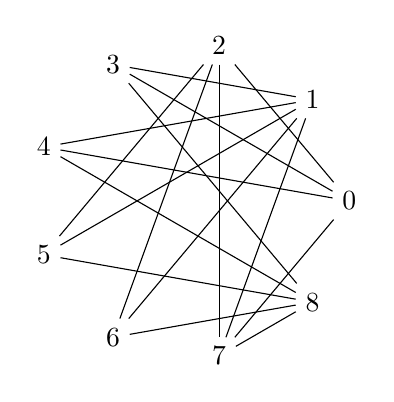
\begin{tikzpicture}
      \draw
        (0.0:2) node (0){0}
        (40.0:2) node (1){1}
        (80.0:2) node (2){2}
        (120.0:2) node (3){3}
        (160.0:2) node (4){4}
        (200.0:2) node (5){5}
        (240.0:2) node (6){6}
        (280.0:2) node (7){7}
        (320.0:2) node (8){8};
      \begin{scope}[-]
        \draw (0) to (2);
        \draw (0) to (3);
        \draw (0) to (4);
        \draw (0) to (7);
        \draw (1) to (3);
        \draw (1) to (4);
        \draw (1) to (5);
        \draw (1) to (6);
        \draw (1) to (7);
        \draw (2) to (5);
        \draw (2) to (6);
        \draw (2) to (7);
        \draw (3) to (8);
        \draw (4) to (8);
        \draw (5) to (8);
        \draw (6) to (8);
        \draw (7) to (8);
      \end{scope}
    \end{tikzpicture}
\end{figure}
\begin{itemize}
\item signature: 011100100111110001110000010001001011
\item g: Graph with 9 nodes and 17 edges
\item order: 9
\item size: 17
\item max degree: 5
\item degrees: 3,3,3,3,4,4,4,5,5
\item is tree: 0
\item is bipartite: 0
\item has bridge: 0
\item is chordal: 0
\item is complete: 0
\item min cycle basis weight: 35
\item min cycle basis size: 9
\item diameter: 2
\item radius: 2
\item is eulerian: 0
\item is planar: 0
\item number of faces: 10
\item is regular: 0
\item p3: 47
\item p4: 36
\item property hash: 57ffa5415fb6a21a0f1df71f3e92fc20d15b5ad909cdb220277fcd2bd7fa672b
\end{itemize}
\newpage
\begin{figure}
  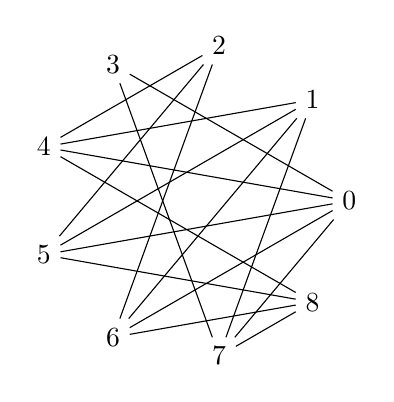
\begin{tikzpicture}
      \draw
        (0.0:2) node (0){0}
        (40.0:2) node (1){1}
        (80.0:2) node (2){2}
        (120.0:2) node (3){3}
        (160.0:2) node (4){4}
        (200.0:2) node (5){5}
        (240.0:2) node (6){6}
        (280.0:2) node (7){7}
        (320.0:2) node (8){8};
      \begin{scope}[-]
        \draw (0) to (3);
        \draw (0) to (4);
        \draw (0) to (5);
        \draw (0) to (6);
        \draw (0) to (7);
        \draw (1) to (4);
        \draw (1) to (5);
        \draw (1) to (6);
        \draw (1) to (7);
        \draw (2) to (4);
        \draw (2) to (5);
        \draw (2) to (6);
        \draw (3) to (7);
        \draw (4) to (8);
        \draw (5) to (8);
        \draw (6) to (8);
        \draw (7) to (8);
      \end{scope}
    \end{tikzpicture}
\end{figure}
\begin{itemize}
\item signature: 001111100011110011100000100001001011
\item g: Graph with 9 nodes and 17 edges
\item order: 9
\item size: 17
\item max degree: 5
\item degrees: 2,3,4,4,4,4,4,4,5
\item is tree: 0
\item is bipartite: 0
\item has bridge: 0
\item is chordal: 0
\item is complete: 0
\item min cycle basis weight: 35
\item min cycle basis size: 9
\item diameter: 3
\item radius: 2
\item is eulerian: 0
\item is planar: 0
\item number of faces: 10
\item is regular: 0
\item p3: 47
\item p4: 24
\item property hash: 1f873b2ce9492d36c6786d7c223216544d79157c0621b32bef3749192035b77e
\end{itemize}
\newpage
\begin{figure}
  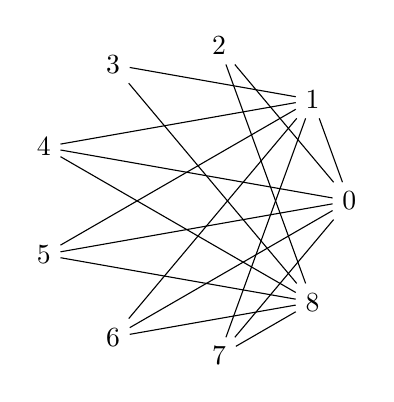
\begin{tikzpicture}
      \draw
        (0.0:2) node (0){0}
        (40.0:2) node (1){1}
        (80.0:2) node (2){2}
        (120.0:2) node (3){3}
        (160.0:2) node (4){4}
        (200.0:2) node (5){5}
        (240.0:2) node (6){6}
        (280.0:2) node (7){7}
        (320.0:2) node (8){8};
      \begin{scope}[-]
        \draw (0) to (1);
        \draw (0) to (2);
        \draw (0) to (4);
        \draw (0) to (5);
        \draw (0) to (6);
        \draw (0) to (7);
        \draw (1) to (3);
        \draw (1) to (4);
        \draw (1) to (5);
        \draw (1) to (6);
        \draw (1) to (7);
        \draw (2) to (8);
        \draw (3) to (8);
        \draw (4) to (8);
        \draw (5) to (8);
        \draw (6) to (8);
        \draw (7) to (8);
      \end{scope}
    \end{tikzpicture}
\end{figure}
\begin{itemize}
\item signature: 110111100111110000001000010001001011
\item g: Graph with 9 nodes and 17 edges
\item order: 9
\item size: 17
\item max degree: 6
\item degrees: 2,2,3,3,3,3,6,6,6
\item is tree: 0
\item is bipartite: 0
\item has bridge: 0
\item is chordal: 0
\item is complete: 0
\item min cycle basis weight: 32
\item min cycle basis size: 9
\item diameter: 2
\item radius: 2
\item is eulerian: 0
\item is planar: 0
\item number of faces: 10
\item is regular: 0
\item p3: 47
\item p4: 13
\item property hash: a40fd5a50aeafc7c0ac210fe90873d9ece95a65b1424babf045b6fbe3e196b9c
\end{itemize}
\newpage
\begin{figure}
  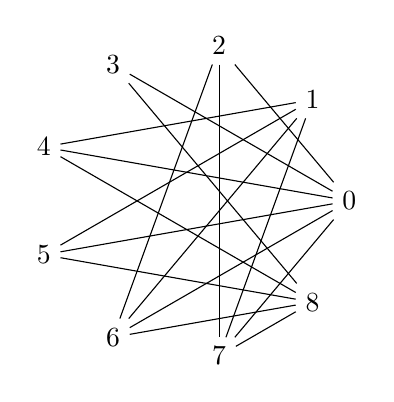
\begin{tikzpicture}
      \draw
        (0.0:2) node (0){0}
        (40.0:2) node (1){1}
        (80.0:2) node (2){2}
        (120.0:2) node (3){3}
        (160.0:2) node (4){4}
        (200.0:2) node (5){5}
        (240.0:2) node (6){6}
        (280.0:2) node (7){7}
        (320.0:2) node (8){8};
      \begin{scope}[-]
        \draw (0) to (2);
        \draw (0) to (3);
        \draw (0) to (4);
        \draw (0) to (5);
        \draw (0) to (6);
        \draw (0) to (7);
        \draw (1) to (4);
        \draw (1) to (5);
        \draw (1) to (6);
        \draw (1) to (7);
        \draw (2) to (6);
        \draw (2) to (7);
        \draw (3) to (8);
        \draw (4) to (8);
        \draw (5) to (8);
        \draw (6) to (8);
        \draw (7) to (8);
      \end{scope}
    \end{tikzpicture}
\end{figure}
\begin{itemize}
\item signature: 011111100011110000110000010001001011
\item g: Graph with 9 nodes and 17 edges
\item order: 9
\item size: 17
\item max degree: 6
\item degrees: 2,3,3,3,4,4,4,5,6
\item is tree: 0
\item is bipartite: 0
\item has bridge: 0
\item is chordal: 0
\item is complete: 0
\item min cycle basis weight: 34
\item min cycle basis size: 9
\item diameter: 3
\item radius: 2
\item is eulerian: 0
\item is planar: 0
\item number of faces: 10
\item is regular: 0
\item p3: 47
\item p4: 23
\item property hash: a204aa92b6488d54f72c013fd1e5cf121bb0a1785240afa5e502c1ffba124872
\end{itemize}
\newpage
\begin{figure}
  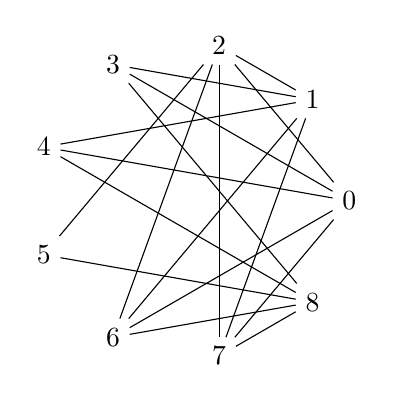
\begin{tikzpicture}
      \draw
        (0.0:2) node (0){0}
        (40.0:2) node (1){1}
        (80.0:2) node (2){2}
        (120.0:2) node (3){3}
        (160.0:2) node (4){4}
        (200.0:2) node (5){5}
        (240.0:2) node (6){6}
        (280.0:2) node (7){7}
        (320.0:2) node (8){8};
      \begin{scope}[-]
        \draw (0) to (2);
        \draw (0) to (3);
        \draw (0) to (4);
        \draw (0) to (6);
        \draw (0) to (7);
        \draw (1) to (2);
        \draw (1) to (3);
        \draw (1) to (4);
        \draw (1) to (6);
        \draw (1) to (7);
        \draw (2) to (5);
        \draw (2) to (6);
        \draw (2) to (7);
        \draw (3) to (8);
        \draw (4) to (8);
        \draw (5) to (8);
        \draw (6) to (8);
        \draw (7) to (8);
      \end{scope}
    \end{tikzpicture}
\end{figure}
\begin{itemize}
\item signature: 011101101110110001110000010001001011
\item g: Graph with 9 nodes and 18 edges
\item order: 9
\item size: 18
\item max degree: 5
\item degrees: 2,3,3,4,4,5,5,5,5
\item is tree: 0
\item is bipartite: 0
\item has bridge: 0
\item is chordal: 0
\item is complete: 0
\item min cycle basis weight: 36
\item min cycle basis size: 10
\item diameter: 2
\item radius: 2
\item is eulerian: 0
\item is planar: 0
\item number of faces: 11
\item is regular: 0
\item p3: 47
\item p4: 24
\item property hash: eb852ff5b3624d4d18c0d9031c142de5058095e95f6fbc0ef9eda7c11bac6262
\end{itemize}
\newpage
\begin{figure}
  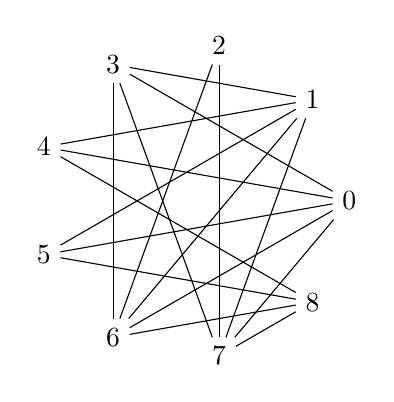
\begin{tikzpicture}
      \draw
        (0.0:2) node (0){0}
        (40.0:2) node (1){1}
        (80.0:2) node (2){2}
        (120.0:2) node (3){3}
        (160.0:2) node (4){4}
        (200.0:2) node (5){5}
        (240.0:2) node (6){6}
        (280.0:2) node (7){7}
        (320.0:2) node (8){8};
      \begin{scope}[-]
        \draw (0) to (3);
        \draw (0) to (4);
        \draw (0) to (5);
        \draw (0) to (6);
        \draw (0) to (7);
        \draw (1) to (3);
        \draw (1) to (4);
        \draw (1) to (5);
        \draw (1) to (6);
        \draw (1) to (7);
        \draw (2) to (6);
        \draw (2) to (7);
        \draw (3) to (6);
        \draw (3) to (7);
        \draw (4) to (8);
        \draw (5) to (8);
        \draw (6) to (8);
        \draw (7) to (8);
      \end{scope}
    \end{tikzpicture}
\end{figure}
\begin{itemize}
\item signature: 001111100111110000110001100001001011
\item g: Graph with 9 nodes and 18 edges
\item order: 9
\item size: 18
\item max degree: 5
\item degrees: 2,3,3,4,4,5,5,5,5
\item is tree: 0
\item is bipartite: 0
\item has bridge: 0
\item is chordal: 0
\item is complete: 0
\item min cycle basis weight: 36
\item min cycle basis size: 10
\item diameter: 3
\item radius: 2
\item is eulerian: 0
\item is planar: 0
\item number of faces: 11
\item is regular: 0
\item p3: 47
\item p4: 20
\item property hash: e698e77459e2a52e290427b37e36aa29a5cda782bfd82f5131454fb9bb7574e1
\end{itemize}
\newpage
\begin{figure}
  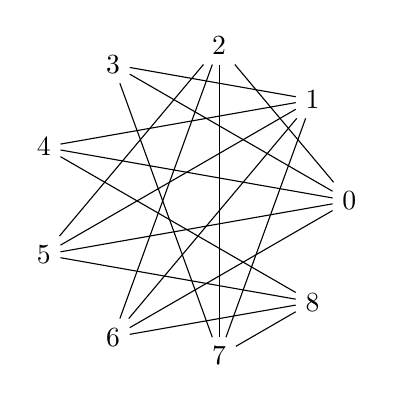
\begin{tikzpicture}
      \draw
        (0.0:2) node (0){0}
        (40.0:2) node (1){1}
        (80.0:2) node (2){2}
        (120.0:2) node (3){3}
        (160.0:2) node (4){4}
        (200.0:2) node (5){5}
        (240.0:2) node (6){6}
        (280.0:2) node (7){7}
        (320.0:2) node (8){8};
      \begin{scope}[-]
        \draw (0) to (2);
        \draw (0) to (3);
        \draw (0) to (4);
        \draw (0) to (5);
        \draw (0) to (6);
        \draw (1) to (3);
        \draw (1) to (4);
        \draw (1) to (5);
        \draw (1) to (6);
        \draw (1) to (7);
        \draw (2) to (5);
        \draw (2) to (6);
        \draw (2) to (7);
        \draw (3) to (7);
        \draw (4) to (8);
        \draw (5) to (8);
        \draw (6) to (8);
        \draw (7) to (8);
      \end{scope}
    \end{tikzpicture}
\end{figure}
\begin{itemize}
\item signature: 011111000111110001110000100001001011
\item g: Graph with 9 nodes and 18 edges
\item order: 9
\item size: 18
\item max degree: 5
\item degrees: 3,3,4,4,4,4,4,5,5
\item is tree: 0
\item is bipartite: 0
\item has bridge: 0
\item is chordal: 0
\item is complete: 0
\item min cycle basis weight: 37
\item min cycle basis size: 10
\item diameter: 2
\item radius: 2
\item is eulerian: 0
\item is planar: 0
\item number of faces: 11
\item is regular: 0
\item p3: 47
\item p4: 35
\item property hash: 870f954ed775daa35015ea0e94f3986463f706134b78a054c72f23524991bd11
\end{itemize}
\newpage
\begin{figure}
  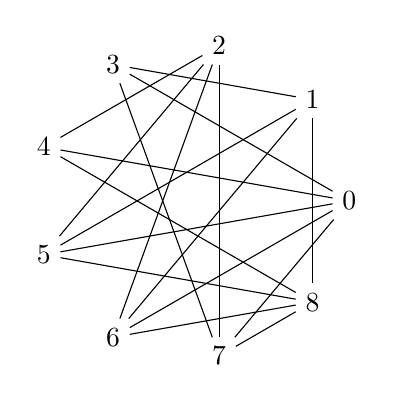
\begin{tikzpicture}
      \draw
        (0.0:2) node (0){0}
        (40.0:2) node (1){1}
        (80.0:2) node (2){2}
        (120.0:2) node (3){3}
        (160.0:2) node (4){4}
        (200.0:2) node (5){5}
        (240.0:2) node (6){6}
        (280.0:2) node (7){7}
        (320.0:2) node (8){8};
      \begin{scope}[-]
        \draw (0) to (3);
        \draw (0) to (4);
        \draw (0) to (5);
        \draw (0) to (6);
        \draw (0) to (7);
        \draw (1) to (3);
        \draw (1) to (5);
        \draw (1) to (6);
        \draw (1) to (8);
        \draw (2) to (4);
        \draw (2) to (5);
        \draw (2) to (6);
        \draw (2) to (7);
        \draw (3) to (7);
        \draw (4) to (8);
        \draw (5) to (8);
        \draw (6) to (8);
        \draw (7) to (8);
      \end{scope}
    \end{tikzpicture}
\end{figure}
\begin{itemize}
\item signature: 001111100101101011110000100001001011
\item g: Graph with 9 nodes and 18 edges
\item order: 9
\item size: 18
\item max degree: 5
\item degrees: 3,3,4,4,4,4,4,5,5
\item is tree: 0
\item is bipartite: 0
\item has bridge: 0
\item is chordal: 0
\item is complete: 0
\item min cycle basis weight: 37
\item min cycle basis size: 10
\item diameter: 2
\item radius: 2
\item is eulerian: 0
\item is planar: 0
\item number of faces: 11
\item is regular: 0
\item p3: 47
\item p4: 32
\item property hash: 66f3f131f1ff0359e5b57745fed4efe065297bd3c42af0ee89c55c9ee8f232c0
\end{itemize}
\newpage
\begin{figure}
  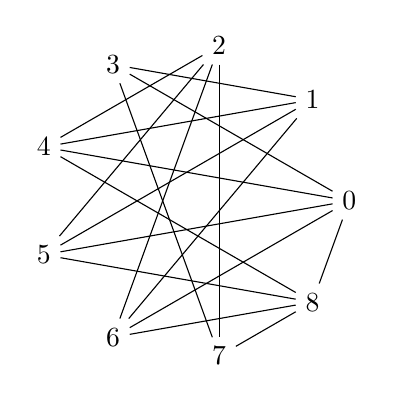
\begin{tikzpicture}
      \draw
        (0.0:2) node (0){0}
        (40.0:2) node (1){1}
        (80.0:2) node (2){2}
        (120.0:2) node (3){3}
        (160.0:2) node (4){4}
        (200.0:2) node (5){5}
        (240.0:2) node (6){6}
        (280.0:2) node (7){7}
        (320.0:2) node (8){8};
      \begin{scope}[-]
        \draw (0) to (3);
        \draw (0) to (4);
        \draw (0) to (5);
        \draw (0) to (6);
        \draw (0) to (8);
        \draw (1) to (3);
        \draw (1) to (4);
        \draw (1) to (5);
        \draw (1) to (6);
        \draw (2) to (4);
        \draw (2) to (5);
        \draw (2) to (6);
        \draw (2) to (7);
        \draw (3) to (7);
        \draw (4) to (8);
        \draw (5) to (8);
        \draw (6) to (8);
        \draw (7) to (8);
      \end{scope}
    \end{tikzpicture}
\end{figure}
\begin{itemize}
\item signature: 001111010111100011110000100001001011
\item g: Graph with 9 nodes and 18 edges
\item order: 9
\item size: 18
\item max degree: 5
\item degrees: 3,3,4,4,4,4,4,5,5
\item is tree: 0
\item is bipartite: 0
\item has bridge: 0
\item is chordal: 0
\item is complete: 0
\item min cycle basis weight: 37
\item min cycle basis size: 10
\item diameter: 2
\item radius: 2
\item is eulerian: 0
\item is planar: 0
\item number of faces: 11
\item is regular: 0
\item p3: 47
\item p4: 35
\item property hash: 870f954ed775daa35015ea0e94f3986463f706134b78a054c72f23524991bd11
\end{itemize}
\newpage
\begin{figure}
  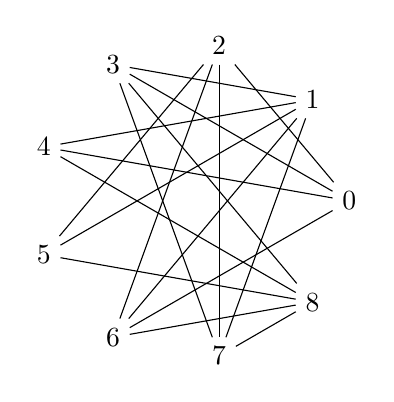
\begin{tikzpicture}
      \draw
        (0.0:2) node (0){0}
        (40.0:2) node (1){1}
        (80.0:2) node (2){2}
        (120.0:2) node (3){3}
        (160.0:2) node (4){4}
        (200.0:2) node (5){5}
        (240.0:2) node (6){6}
        (280.0:2) node (7){7}
        (320.0:2) node (8){8};
      \begin{scope}[-]
        \draw (0) to (2);
        \draw (0) to (3);
        \draw (0) to (4);
        \draw (0) to (6);
        \draw (1) to (3);
        \draw (1) to (4);
        \draw (1) to (5);
        \draw (1) to (6);
        \draw (1) to (7);
        \draw (2) to (5);
        \draw (2) to (6);
        \draw (2) to (7);
        \draw (3) to (7);
        \draw (3) to (8);
        \draw (4) to (8);
        \draw (5) to (8);
        \draw (6) to (8);
        \draw (7) to (8);
      \end{scope}
    \end{tikzpicture}
\end{figure}
\begin{itemize}
\item signature: 011101000111110001110000110001001011
\item g: Graph with 9 nodes and 18 edges
\item order: 9
\item size: 18
\item max degree: 5
\item degrees: 3,3,4,4,4,4,4,5,5
\item is tree: 0
\item is bipartite: 0
\item has bridge: 0
\item is chordal: 0
\item is complete: 0
\item min cycle basis weight: 37
\item min cycle basis size: 10
\item diameter: 2
\item radius: 2
\item is eulerian: 0
\item is planar: 0
\item number of faces: 11
\item is regular: 0
\item p3: 47
\item p4: 35
\item property hash: 870f954ed775daa35015ea0e94f3986463f706134b78a054c72f23524991bd11
\end{itemize}
\newpage
\begin{figure}
  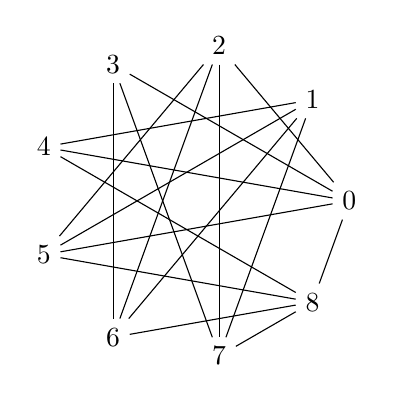
\begin{tikzpicture}
      \draw
        (0.0:2) node (0){0}
        (40.0:2) node (1){1}
        (80.0:2) node (2){2}
        (120.0:2) node (3){3}
        (160.0:2) node (4){4}
        (200.0:2) node (5){5}
        (240.0:2) node (6){6}
        (280.0:2) node (7){7}
        (320.0:2) node (8){8};
      \begin{scope}[-]
        \draw (0) to (2);
        \draw (0) to (3);
        \draw (0) to (4);
        \draw (0) to (5);
        \draw (0) to (8);
        \draw (1) to (4);
        \draw (1) to (5);
        \draw (1) to (6);
        \draw (1) to (7);
        \draw (2) to (5);
        \draw (2) to (6);
        \draw (2) to (7);
        \draw (3) to (6);
        \draw (3) to (7);
        \draw (4) to (8);
        \draw (5) to (8);
        \draw (6) to (8);
        \draw (7) to (8);
      \end{scope}
    \end{tikzpicture}
\end{figure}
\begin{itemize}
\item signature: 011110010011110001110001100001001011
\item g: Graph with 9 nodes and 18 edges
\item order: 9
\item size: 18
\item max degree: 5
\item degrees: 3,3,4,4,4,4,4,5,5
\item is tree: 0
\item is bipartite: 0
\item has bridge: 0
\item is chordal: 0
\item is complete: 0
\item min cycle basis weight: 37
\item min cycle basis size: 10
\item diameter: 2
\item radius: 2
\item is eulerian: 0
\item is planar: 0
\item number of faces: 11
\item is regular: 0
\item p3: 47
\item p4: 35
\item property hash: 870f954ed775daa35015ea0e94f3986463f706134b78a054c72f23524991bd11
\end{itemize}
\newpage
\begin{figure}
  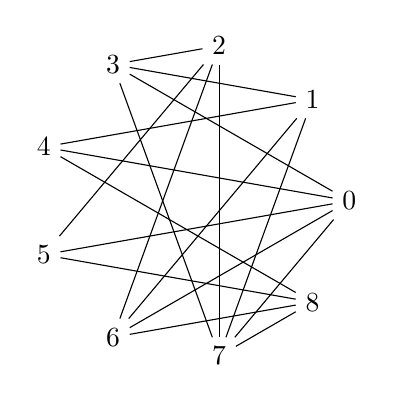
\begin{tikzpicture}
      \draw
        (0.0:2) node (0){0}
        (40.0:2) node (1){1}
        (80.0:2) node (2){2}
        (120.0:2) node (3){3}
        (160.0:2) node (4){4}
        (200.0:2) node (5){5}
        (240.0:2) node (6){6}
        (280.0:2) node (7){7}
        (320.0:2) node (8){8};
      \begin{scope}[-]
        \draw (0) to (3);
        \draw (0) to (4);
        \draw (0) to (5);
        \draw (0) to (6);
        \draw (0) to (7);
        \draw (1) to (3);
        \draw (1) to (4);
        \draw (1) to (6);
        \draw (1) to (7);
        \draw (2) to (3);
        \draw (2) to (5);
        \draw (2) to (6);
        \draw (2) to (7);
        \draw (3) to (7);
        \draw (4) to (8);
        \draw (5) to (8);
        \draw (6) to (8);
        \draw (7) to (8);
      \end{scope}
    \end{tikzpicture}
\end{figure}
\begin{itemize}
\item signature: 001111100110110101110000100001001011
\item g: Graph with 9 nodes and 18 edges
\item order: 9
\item size: 18
\item max degree: 5
\item degrees: 3,3,4,4,4,4,4,5,5
\item is tree: 0
\item is bipartite: 0
\item has bridge: 0
\item is chordal: 0
\item is complete: 0
\item min cycle basis weight: 37
\item min cycle basis size: 10
\item diameter: 3
\item radius: 2
\item is eulerian: 0
\item is planar: 0
\item number of faces: 11
\item is regular: 0
\item p3: 47
\item p4: 30
\item property hash: 751a6af9cbc0955e4b18568e19ab486122a6da9c4ced49530a4fc9401d8629e2
\end{itemize}
\newpage
\begin{figure}
  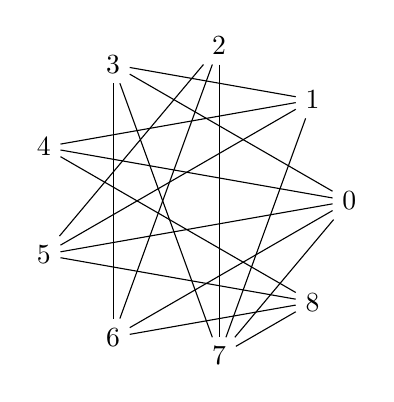
\begin{tikzpicture}
      \draw
        (0.0:2) node (0){0}
        (40.0:2) node (1){1}
        (80.0:2) node (2){2}
        (120.0:2) node (3){3}
        (160.0:2) node (4){4}
        (200.0:2) node (5){5}
        (240.0:2) node (6){6}
        (280.0:2) node (7){7}
        (320.0:2) node (8){8};
      \begin{scope}[-]
        \draw (0) to (3);
        \draw (0) to (4);
        \draw (0) to (5);
        \draw (0) to (6);
        \draw (0) to (7);
        \draw (1) to (3);
        \draw (1) to (4);
        \draw (1) to (5);
        \draw (1) to (7);
        \draw (2) to (5);
        \draw (2) to (6);
        \draw (2) to (7);
        \draw (3) to (6);
        \draw (3) to (7);
        \draw (4) to (8);
        \draw (5) to (8);
        \draw (6) to (8);
        \draw (7) to (8);
      \end{scope}
    \end{tikzpicture}
\end{figure}
\begin{itemize}
\item signature: 001111100111010001110001100001001011
\item g: Graph with 9 nodes and 18 edges
\item order: 9
\item size: 18
\item max degree: 5
\item degrees: 3,3,4,4,4,4,4,5,5
\item is tree: 0
\item is bipartite: 0
\item has bridge: 0
\item is chordal: 0
\item is complete: 0
\item min cycle basis weight: 37
\item min cycle basis size: 10
\item diameter: 3
\item radius: 2
\item is eulerian: 0
\item is planar: 0
\item number of faces: 11
\item is regular: 0
\item p3: 47
\item p4: 32
\item property hash: 8bc79dfb9589a76d7b6baae0a6cb85351a020ba396bf51b4d04ced15f36bc732
\end{itemize}
\newpage
\begin{figure}
  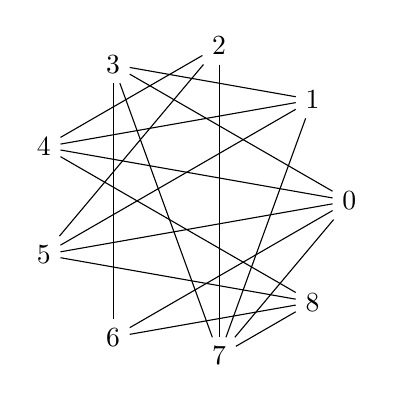
\begin{tikzpicture}
      \draw
        (0.0:2) node (0){0}
        (40.0:2) node (1){1}
        (80.0:2) node (2){2}
        (120.0:2) node (3){3}
        (160.0:2) node (4){4}
        (200.0:2) node (5){5}
        (240.0:2) node (6){6}
        (280.0:2) node (7){7}
        (320.0:2) node (8){8};
      \begin{scope}[-]
        \draw (0) to (3);
        \draw (0) to (4);
        \draw (0) to (5);
        \draw (0) to (6);
        \draw (0) to (7);
        \draw (1) to (3);
        \draw (1) to (4);
        \draw (1) to (5);
        \draw (1) to (7);
        \draw (2) to (4);
        \draw (2) to (5);
        \draw (2) to (7);
        \draw (3) to (6);
        \draw (3) to (7);
        \draw (4) to (8);
        \draw (5) to (8);
        \draw (6) to (8);
        \draw (7) to (8);
      \end{scope}
    \end{tikzpicture}
\end{figure}
\begin{itemize}
\item signature: 001111100111010011010001100001001011
\item g: Graph with 9 nodes and 18 edges
\item order: 9
\item size: 18
\item max degree: 5
\item degrees: 3,3,4,4,4,4,4,5,5
\item is tree: 0
\item is bipartite: 0
\item has bridge: 0
\item is chordal: 0
\item is complete: 0
\item min cycle basis weight: 37
\item min cycle basis size: 10
\item diameter: 3
\item radius: 2
\item is eulerian: 0
\item is planar: 0
\item number of faces: 11
\item is regular: 0
\item p3: 47
\item p4: 30
\item property hash: 751a6af9cbc0955e4b18568e19ab486122a6da9c4ced49530a4fc9401d8629e2
\end{itemize}
\newpage
\begin{figure}
  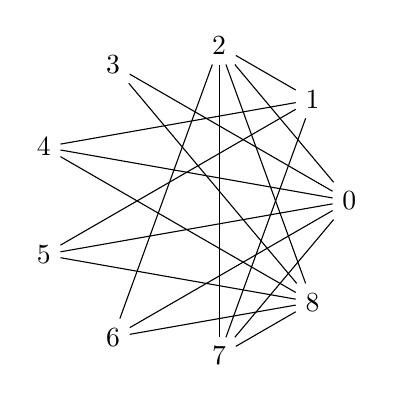
\begin{tikzpicture}
      \draw
        (0.0:2) node (0){0}
        (40.0:2) node (1){1}
        (80.0:2) node (2){2}
        (120.0:2) node (3){3}
        (160.0:2) node (4){4}
        (200.0:2) node (5){5}
        (240.0:2) node (6){6}
        (280.0:2) node (7){7}
        (320.0:2) node (8){8};
      \begin{scope}[-]
        \draw (0) to (2);
        \draw (0) to (3);
        \draw (0) to (4);
        \draw (0) to (5);
        \draw (0) to (6);
        \draw (0) to (7);
        \draw (1) to (2);
        \draw (1) to (4);
        \draw (1) to (5);
        \draw (1) to (7);
        \draw (2) to (6);
        \draw (2) to (7);
        \draw (2) to (8);
        \draw (3) to (8);
        \draw (4) to (8);
        \draw (5) to (8);
        \draw (6) to (8);
        \draw (7) to (8);
      \end{scope}
    \end{tikzpicture}
\end{figure}
\begin{itemize}
\item signature: 011111101011010000111000010001001011
\item g: Graph with 9 nodes and 18 edges
\item order: 9
\item size: 18
\item max degree: 6
\item degrees: 2,3,3,3,4,4,5,6,6
\item is tree: 0
\item is bipartite: 0
\item has bridge: 0
\item is chordal: 0
\item is complete: 0
\item min cycle basis weight: 35
\item min cycle basis size: 10
\item diameter: 3
\item radius: 2
\item is eulerian: 0
\item is planar: 0
\item number of faces: 11
\item is regular: 0
\item p3: 47
\item p4: None
\item property hash: 90f8999de7a0bec1184fcccea03e961e717de988ae69c6b021517db2f3bfaaeb
\end{itemize}
\newpage
\begin{figure}
  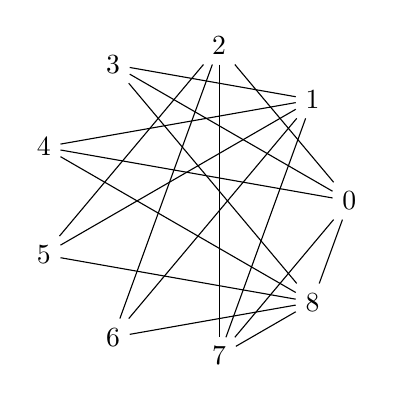
\begin{tikzpicture}
      \draw
        (0.0:2) node (0){0}
        (40.0:2) node (1){1}
        (80.0:2) node (2){2}
        (120.0:2) node (3){3}
        (160.0:2) node (4){4}
        (200.0:2) node (5){5}
        (240.0:2) node (6){6}
        (280.0:2) node (7){7}
        (320.0:2) node (8){8};
      \begin{scope}[-]
        \draw (0) to (2);
        \draw (0) to (3);
        \draw (0) to (4);
        \draw (0) to (7);
        \draw (0) to (8);
        \draw (1) to (3);
        \draw (1) to (4);
        \draw (1) to (5);
        \draw (1) to (6);
        \draw (1) to (7);
        \draw (2) to (5);
        \draw (2) to (6);
        \draw (2) to (7);
        \draw (3) to (8);
        \draw (4) to (8);
        \draw (5) to (8);
        \draw (6) to (8);
        \draw (7) to (8);
      \end{scope}
    \end{tikzpicture}
\end{figure}
\begin{itemize}
\item signature: 011100110111110001110000010001001011
\item g: Graph with 9 nodes and 18 edges
\item order: 9
\item size: 18
\item max degree: 6
\item degrees: 3,3,3,3,4,4,5,5,6
\item is tree: 0
\item is bipartite: 0
\item has bridge: 0
\item is chordal: 0
\item is complete: 0
\item min cycle basis weight: 36
\item min cycle basis size: 10
\item diameter: 2
\item radius: 2
\item is eulerian: 0
\item is planar: 0
\item number of faces: 11
\item is regular: 0
\item p3: 47
\item p4: 28
\item property hash: 2f13044ad2756a72062042331cf46df1d694f567d211c5b1839fa32dc247bec1
\end{itemize}
\newpage
\begin{figure}
  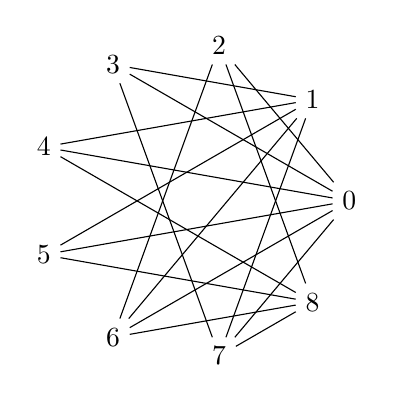
\begin{tikzpicture}
      \draw
        (0.0:2) node (0){0}
        (40.0:2) node (1){1}
        (80.0:2) node (2){2}
        (120.0:2) node (3){3}
        (160.0:2) node (4){4}
        (200.0:2) node (5){5}
        (240.0:2) node (6){6}
        (280.0:2) node (7){7}
        (320.0:2) node (8){8};
      \begin{scope}[-]
        \draw (0) to (2);
        \draw (0) to (3);
        \draw (0) to (4);
        \draw (0) to (5);
        \draw (0) to (6);
        \draw (0) to (7);
        \draw (1) to (3);
        \draw (1) to (4);
        \draw (1) to (5);
        \draw (1) to (6);
        \draw (1) to (7);
        \draw (2) to (6);
        \draw (2) to (8);
        \draw (3) to (7);
        \draw (4) to (8);
        \draw (5) to (8);
        \draw (6) to (8);
        \draw (7) to (8);
      \end{scope}
    \end{tikzpicture}
\end{figure}
\begin{itemize}
\item signature: 011111100111110000101000100001001011
\item g: Graph with 9 nodes and 18 edges
\item order: 9
\item size: 18
\item max degree: 6
\item degrees: 3,3,3,3,4,4,5,5,6
\item is tree: 0
\item is bipartite: 0
\item has bridge: 0
\item is chordal: 0
\item is complete: 0
\item min cycle basis weight: 36
\item min cycle basis size: 10
\item diameter: 2
\item radius: 2
\item is eulerian: 0
\item is planar: 0
\item number of faces: 11
\item is regular: 0
\item p3: 47
\item p4: 22
\item property hash: a2f6e71a02188df4dac834b592137f2ccc6d40f8d9e519e05fd7efdb6eae5542
\end{itemize}
\newpage
\begin{figure}
  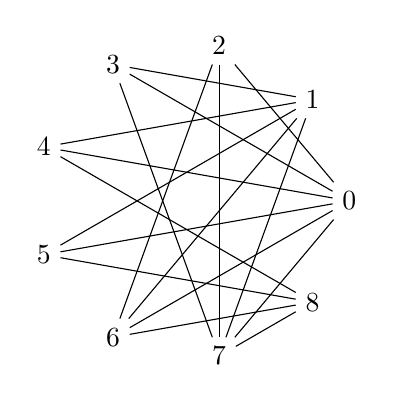
\begin{tikzpicture}
      \draw
        (0.0:2) node (0){0}
        (40.0:2) node (1){1}
        (80.0:2) node (2){2}
        (120.0:2) node (3){3}
        (160.0:2) node (4){4}
        (200.0:2) node (5){5}
        (240.0:2) node (6){6}
        (280.0:2) node (7){7}
        (320.0:2) node (8){8};
      \begin{scope}[-]
        \draw (0) to (2);
        \draw (0) to (3);
        \draw (0) to (4);
        \draw (0) to (5);
        \draw (0) to (6);
        \draw (0) to (7);
        \draw (1) to (3);
        \draw (1) to (4);
        \draw (1) to (5);
        \draw (1) to (6);
        \draw (1) to (7);
        \draw (2) to (6);
        \draw (2) to (7);
        \draw (3) to (7);
        \draw (4) to (8);
        \draw (5) to (8);
        \draw (6) to (8);
        \draw (7) to (8);
      \end{scope}
    \end{tikzpicture}
\end{figure}
\begin{itemize}
\item signature: 011111100111110000110000100001001011
\item g: Graph with 9 nodes and 18 edges
\item order: 9
\item size: 18
\item max degree: 6
\item degrees: 3,3,3,3,4,4,5,5,6
\item is tree: 0
\item is bipartite: 0
\item has bridge: 0
\item is chordal: 0
\item is complete: 0
\item min cycle basis weight: 36
\item min cycle basis size: 10
\item diameter: 2
\item radius: 2
\item is eulerian: 0
\item is planar: 0
\item number of faces: 11
\item is regular: 0
\item p3: 47
\item p4: None
\item property hash: 91d2af92a6501e98ff1cc68e696c4e828374a92692c5936a775968329de6e35c
\end{itemize}
\newpage
\begin{figure}
  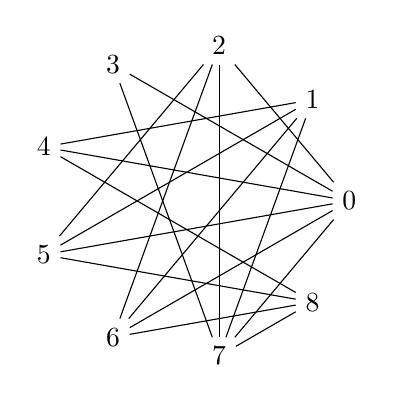
\begin{tikzpicture}
      \draw
        (0.0:2) node (0){0}
        (40.0:2) node (1){1}
        (80.0:2) node (2){2}
        (120.0:2) node (3){3}
        (160.0:2) node (4){4}
        (200.0:2) node (5){5}
        (240.0:2) node (6){6}
        (280.0:2) node (7){7}
        (320.0:2) node (8){8};
      \begin{scope}[-]
        \draw (0) to (2);
        \draw (0) to (3);
        \draw (0) to (4);
        \draw (0) to (5);
        \draw (0) to (6);
        \draw (0) to (7);
        \draw (1) to (4);
        \draw (1) to (5);
        \draw (1) to (6);
        \draw (1) to (7);
        \draw (2) to (5);
        \draw (2) to (6);
        \draw (2) to (7);
        \draw (3) to (7);
        \draw (4) to (8);
        \draw (5) to (8);
        \draw (6) to (8);
        \draw (7) to (8);
      \end{scope}
    \end{tikzpicture}
\end{figure}
\begin{itemize}
\item signature: 011111100011110001110000100001001011
\item g: Graph with 9 nodes and 18 edges
\item order: 9
\item size: 18
\item max degree: 6
\item degrees: 2,3,4,4,4,4,4,5,6
\item is tree: 0
\item is bipartite: 0
\item has bridge: 0
\item is chordal: 0
\item is complete: 0
\item min cycle basis weight: 36
\item min cycle basis size: 10
\item diameter: 2
\item radius: 2
\item is eulerian: 0
\item is planar: 0
\item number of faces: 11
\item is regular: 0
\item p3: 47
\item p4: None
\item property hash: 3d3d821b973c0c29af391220b42ef2d3082c5389227cd5122106d03cbb27d074
\end{itemize}
\newpage
\begin{figure}
  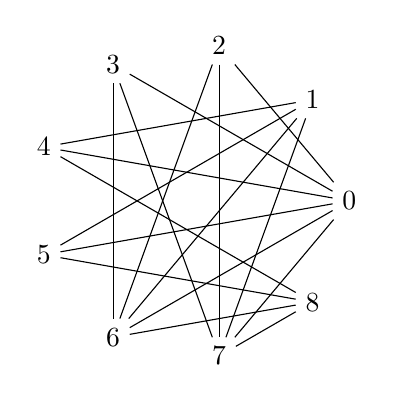
\begin{tikzpicture}
      \draw
        (0.0:2) node (0){0}
        (40.0:2) node (1){1}
        (80.0:2) node (2){2}
        (120.0:2) node (3){3}
        (160.0:2) node (4){4}
        (200.0:2) node (5){5}
        (240.0:2) node (6){6}
        (280.0:2) node (7){7}
        (320.0:2) node (8){8};
      \begin{scope}[-]
        \draw (0) to (2);
        \draw (0) to (3);
        \draw (0) to (4);
        \draw (0) to (5);
        \draw (0) to (6);
        \draw (0) to (7);
        \draw (1) to (4);
        \draw (1) to (5);
        \draw (1) to (6);
        \draw (1) to (7);
        \draw (2) to (6);
        \draw (2) to (7);
        \draw (3) to (6);
        \draw (3) to (7);
        \draw (4) to (8);
        \draw (5) to (8);
        \draw (6) to (8);
        \draw (7) to (8);
      \end{scope}
    \end{tikzpicture}
\end{figure}
\begin{itemize}
\item signature: 011111100011110000110001100001001011
\item g: Graph with 9 nodes and 18 edges
\item order: 9
\item size: 18
\item max degree: 6
\item degrees: 3,3,3,3,4,4,5,5,6
\item is tree: 0
\item is bipartite: 0
\item has bridge: 0
\item is chordal: 0
\item is complete: 0
\item min cycle basis weight: 36
\item min cycle basis size: 10
\item diameter: 2
\item radius: 2
\item is eulerian: 0
\item is planar: 0
\item number of faces: 11
\item is regular: 0
\item p3: 47
\item p4: None
\item property hash: 91d2af92a6501e98ff1cc68e696c4e828374a92692c5936a775968329de6e35c
\end{itemize}
\newpage
\begin{figure}
  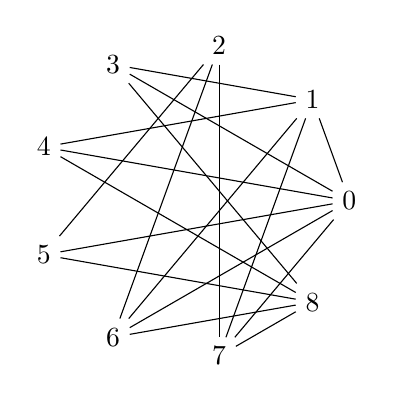
\begin{tikzpicture}
      \draw
        (0.0:2) node (0){0}
        (40.0:2) node (1){1}
        (80.0:2) node (2){2}
        (120.0:2) node (3){3}
        (160.0:2) node (4){4}
        (200.0:2) node (5){5}
        (240.0:2) node (6){6}
        (280.0:2) node (7){7}
        (320.0:2) node (8){8};
      \begin{scope}[-]
        \draw (0) to (1);
        \draw (0) to (3);
        \draw (0) to (4);
        \draw (0) to (5);
        \draw (0) to (6);
        \draw (0) to (7);
        \draw (1) to (3);
        \draw (1) to (4);
        \draw (1) to (6);
        \draw (1) to (7);
        \draw (2) to (5);
        \draw (2) to (6);
        \draw (2) to (7);
        \draw (3) to (8);
        \draw (4) to (8);
        \draw (5) to (8);
        \draw (6) to (8);
        \draw (7) to (8);
      \end{scope}
    \end{tikzpicture}
\end{figure}
\begin{itemize}
\item signature: 101111100110110001110000010001001011
\item g: Graph with 9 nodes and 18 edges
\item order: 9
\item size: 18
\item max degree: 6
\item degrees: 3,3,3,3,4,4,5,5,6
\item is tree: 0
\item is bipartite: 0
\item has bridge: 0
\item is chordal: 0
\item is complete: 0
\item min cycle basis weight: 36
\item min cycle basis size: 10
\item diameter: 3
\item radius: 2
\item is eulerian: 0
\item is planar: 0
\item number of faces: 11
\item is regular: 0
\item p3: 47
\item p4: 24
\item property hash: 793abdb5c630ae7e7055d61ac3b6667fe85c60a49b07da2b0836267aaf918ed9
\end{itemize}
\newpage
\begin{figure}
  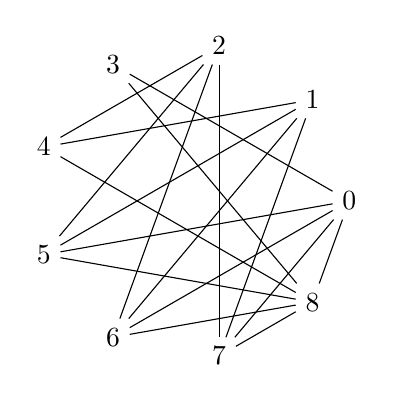
\begin{tikzpicture}
      \draw
        (0.0:2) node (0){0}
        (40.0:2) node (1){1}
        (80.0:2) node (2){2}
        (120.0:2) node (3){3}
        (160.0:2) node (4){4}
        (200.0:2) node (5){5}
        (240.0:2) node (6){6}
        (280.0:2) node (7){7}
        (320.0:2) node (8){8};
      \begin{scope}[-]
        \draw (0) to (3);
        \draw (0) to (5);
        \draw (0) to (6);
        \draw (0) to (7);
        \draw (0) to (8);
        \draw (1) to (4);
        \draw (1) to (5);
        \draw (1) to (6);
        \draw (1) to (7);
        \draw (2) to (4);
        \draw (2) to (5);
        \draw (2) to (6);
        \draw (2) to (7);
        \draw (3) to (8);
        \draw (4) to (8);
        \draw (5) to (8);
        \draw (6) to (8);
        \draw (7) to (8);
      \end{scope}
    \end{tikzpicture}
\end{figure}
\begin{itemize}
\item signature: 001011110011110011110000010001001011
\item g: Graph with 9 nodes and 18 edges
\item order: 9
\item size: 18
\item max degree: 6
\item degrees: 2,3,4,4,4,4,4,5,6
\item is tree: 0
\item is bipartite: 0
\item has bridge: 0
\item is chordal: 0
\item is complete: 0
\item min cycle basis weight: 36
\item min cycle basis size: 10
\item diameter: 3
\item radius: 2
\item is eulerian: 0
\item is planar: 0
\item number of faces: 11
\item is regular: 0
\item p3: 47
\item p4: 22
\item property hash: 9c47db0b42f24955cfad7eca30ebb4792f991fe8365d8cae585eccdce5daedaf
\end{itemize}
\newpage
\begin{figure}
  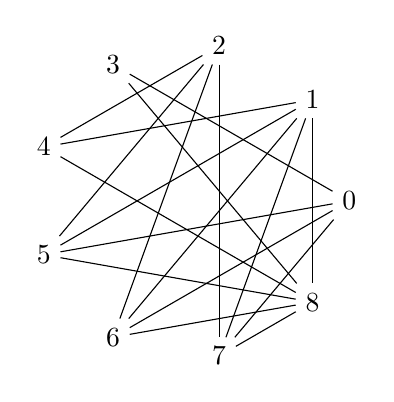
\begin{tikzpicture}
      \draw
        (0.0:2) node (0){0}
        (40.0:2) node (1){1}
        (80.0:2) node (2){2}
        (120.0:2) node (3){3}
        (160.0:2) node (4){4}
        (200.0:2) node (5){5}
        (240.0:2) node (6){6}
        (280.0:2) node (7){7}
        (320.0:2) node (8){8};
      \begin{scope}[-]
        \draw (0) to (3);
        \draw (0) to (5);
        \draw (0) to (6);
        \draw (0) to (7);
        \draw (1) to (4);
        \draw (1) to (5);
        \draw (1) to (6);
        \draw (1) to (7);
        \draw (1) to (8);
        \draw (2) to (4);
        \draw (2) to (5);
        \draw (2) to (6);
        \draw (2) to (7);
        \draw (3) to (8);
        \draw (4) to (8);
        \draw (5) to (8);
        \draw (6) to (8);
        \draw (7) to (8);
      \end{scope}
    \end{tikzpicture}
\end{figure}
\begin{itemize}
\item signature: 001011100011111011110000010001001011
\item g: Graph with 9 nodes and 18 edges
\item order: 9
\item size: 18
\item max degree: 6
\item degrees: 2,3,4,4,4,4,4,5,6
\item is tree: 0
\item is bipartite: 0
\item has bridge: 0
\item is chordal: 0
\item is complete: 0
\item min cycle basis weight: 36
\item min cycle basis size: 10
\item diameter: 3
\item radius: 2
\item is eulerian: 0
\item is planar: 0
\item number of faces: 11
\item is regular: 0
\item p3: 47
\item p4: 21
\item property hash: 3631a4482b85013409501dd262a27f688a08cc05084087257eecffe833dc8185
\end{itemize}
\newpage
\begin{figure}
  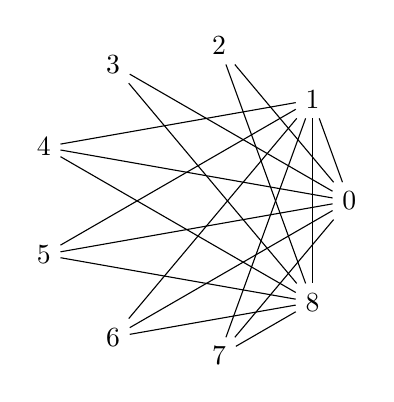
\begin{tikzpicture}
      \draw
        (0.0:2) node (0){0}
        (40.0:2) node (1){1}
        (80.0:2) node (2){2}
        (120.0:2) node (3){3}
        (160.0:2) node (4){4}
        (200.0:2) node (5){5}
        (240.0:2) node (6){6}
        (280.0:2) node (7){7}
        (320.0:2) node (8){8};
      \begin{scope}[-]
        \draw (0) to (1);
        \draw (0) to (2);
        \draw (0) to (3);
        \draw (0) to (4);
        \draw (0) to (5);
        \draw (0) to (6);
        \draw (0) to (7);
        \draw (1) to (4);
        \draw (1) to (5);
        \draw (1) to (6);
        \draw (1) to (7);
        \draw (1) to (8);
        \draw (2) to (8);
        \draw (3) to (8);
        \draw (4) to (8);
        \draw (5) to (8);
        \draw (6) to (8);
        \draw (7) to (8);
      \end{scope}
    \end{tikzpicture}
\end{figure}
\begin{itemize}
\item signature: 111111100011111000001000010001001011
\item g: Graph with 9 nodes and 18 edges
\item order: 9
\item size: 18
\item max degree: 7
\item degrees: 2,2,3,3,3,3,6,7,7
\item is tree: 0
\item is bipartite: 0
\item has bridge: 0
\item is chordal: 0
\item is complete: 0
\item min cycle basis weight: 32
\item min cycle basis size: 10
\item diameter: 2
\item radius: 2
\item is eulerian: 0
\item is planar: 0
\item number of faces: 11
\item is regular: 0
\item p3: 47
\item p4: None
\item property hash: ec330d4067a632b9334363cd1802c0432aa68511c8739666e983de6f6b65db71
\end{itemize}
\newpage
\begin{figure}
  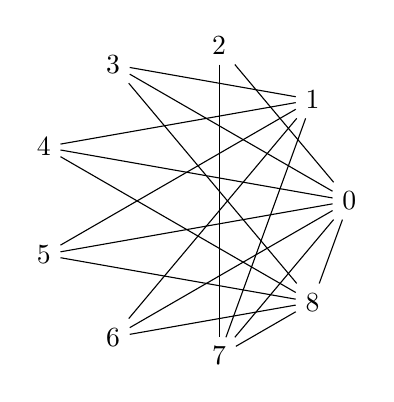
\begin{tikzpicture}
      \draw
        (0.0:2) node (0){0}
        (40.0:2) node (1){1}
        (80.0:2) node (2){2}
        (120.0:2) node (3){3}
        (160.0:2) node (4){4}
        (200.0:2) node (5){5}
        (240.0:2) node (6){6}
        (280.0:2) node (7){7}
        (320.0:2) node (8){8};
      \begin{scope}[-]
        \draw (0) to (2);
        \draw (0) to (3);
        \draw (0) to (4);
        \draw (0) to (5);
        \draw (0) to (6);
        \draw (0) to (7);
        \draw (0) to (8);
        \draw (1) to (3);
        \draw (1) to (4);
        \draw (1) to (5);
        \draw (1) to (6);
        \draw (1) to (7);
        \draw (2) to (7);
        \draw (3) to (8);
        \draw (4) to (8);
        \draw (5) to (8);
        \draw (6) to (8);
        \draw (7) to (8);
      \end{scope}
    \end{tikzpicture}
\end{figure}
\begin{itemize}
\item signature: 011111110111110000010000010001001011
\item g: Graph with 9 nodes and 18 edges
\item order: 9
\item size: 18
\item max degree: 7
\item degrees: 2,3,3,3,3,4,5,6,7
\item is tree: 0
\item is bipartite: 0
\item has bridge: 0
\item is chordal: 0
\item is complete: 0
\item min cycle basis weight: 34
\item min cycle basis size: 10
\item diameter: 2
\item radius: 2
\item is eulerian: 0
\item is planar: 0
\item number of faces: 11
\item is regular: 0
\item p3: 47
\item p4: None
\item property hash: 7d95294acc51c6de39236a98753f4c5d1078989bff29dd0e6ef9f80166bc8120
\end{itemize}
\newpage
\begin{figure}
  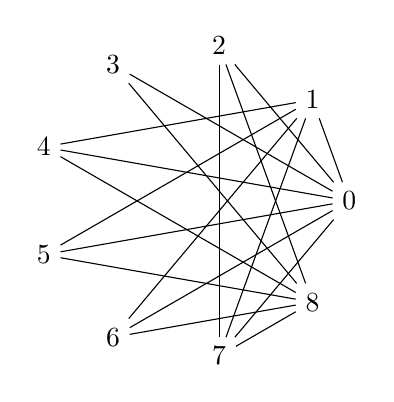
\begin{tikzpicture}
      \draw
        (0.0:2) node (0){0}
        (40.0:2) node (1){1}
        (80.0:2) node (2){2}
        (120.0:2) node (3){3}
        (160.0:2) node (4){4}
        (200.0:2) node (5){5}
        (240.0:2) node (6){6}
        (280.0:2) node (7){7}
        (320.0:2) node (8){8};
      \begin{scope}[-]
        \draw (0) to (1);
        \draw (0) to (2);
        \draw (0) to (3);
        \draw (0) to (4);
        \draw (0) to (5);
        \draw (0) to (6);
        \draw (0) to (7);
        \draw (1) to (4);
        \draw (1) to (5);
        \draw (1) to (6);
        \draw (1) to (7);
        \draw (2) to (7);
        \draw (2) to (8);
        \draw (3) to (8);
        \draw (4) to (8);
        \draw (5) to (8);
        \draw (6) to (8);
        \draw (7) to (8);
      \end{scope}
    \end{tikzpicture}
\end{figure}
\begin{itemize}
\item signature: 111111100011110000011000010001001011
\item g: Graph with 9 nodes and 18 edges
\item order: 9
\item size: 18
\item max degree: 7
\item degrees: 2,3,3,3,3,4,5,6,7
\item is tree: 0
\item is bipartite: 0
\item has bridge: 0
\item is chordal: 0
\item is complete: 0
\item min cycle basis weight: 34
\item min cycle basis size: 10
\item diameter: 2
\item radius: 2
\item is eulerian: 0
\item is planar: 0
\item number of faces: 11
\item is regular: 0
\item p3: 47
\item p4: None
\item property hash: 7d95294acc51c6de39236a98753f4c5d1078989bff29dd0e6ef9f80166bc8120
\end{itemize}
\newpage
\begin{figure}
  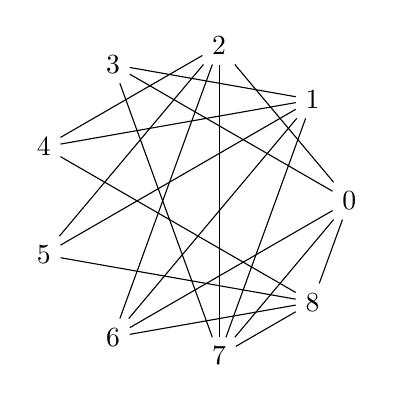
\begin{tikzpicture}
      \draw
        (0.0:2) node (0){0}
        (40.0:2) node (1){1}
        (80.0:2) node (2){2}
        (120.0:2) node (3){3}
        (160.0:2) node (4){4}
        (200.0:2) node (5){5}
        (240.0:2) node (6){6}
        (280.0:2) node (7){7}
        (320.0:2) node (8){8};
      \begin{scope}[-]
        \draw (0) to (2);
        \draw (0) to (3);
        \draw (0) to (6);
        \draw (0) to (7);
        \draw (0) to (8);
        \draw (1) to (3);
        \draw (1) to (4);
        \draw (1) to (5);
        \draw (1) to (6);
        \draw (1) to (7);
        \draw (2) to (4);
        \draw (2) to (5);
        \draw (2) to (6);
        \draw (2) to (7);
        \draw (3) to (7);
        \draw (4) to (8);
        \draw (5) to (8);
        \draw (6) to (8);
        \draw (7) to (8);
      \end{scope}
    \end{tikzpicture}
\end{figure}
\begin{itemize}
\item signature: 011001110111110011110000100001001011
\item g: Graph with 9 nodes and 19 edges
\item order: 9
\item size: 19
\item max degree: 5
\item degrees: 3,3,3,4,5,5,5,5,5
\item is tree: 0
\item is bipartite: 0
\item has bridge: 0
\item is chordal: 0
\item is complete: 0
\item min cycle basis weight: 38
\item min cycle basis size: 11
\item diameter: 2
\item radius: 2
\item is eulerian: 0
\item is planar: 0
\item number of faces: 12
\item is regular: 0
\item p3: 47
\item p4: 28
\item property hash: 94e07c0fa58c39c6cca88a50c901c8b59b83dad012cfdf673928fef976b68a0b
\end{itemize}
\newpage
\begin{figure}
  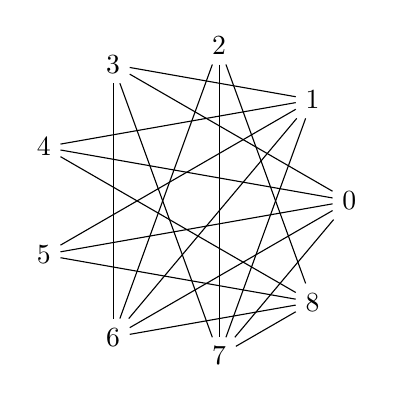
\begin{tikzpicture}
      \draw
        (0.0:2) node (0){0}
        (40.0:2) node (1){1}
        (80.0:2) node (2){2}
        (120.0:2) node (3){3}
        (160.0:2) node (4){4}
        (200.0:2) node (5){5}
        (240.0:2) node (6){6}
        (280.0:2) node (7){7}
        (320.0:2) node (8){8};
      \begin{scope}[-]
        \draw (0) to (3);
        \draw (0) to (4);
        \draw (0) to (5);
        \draw (0) to (6);
        \draw (0) to (7);
        \draw (1) to (3);
        \draw (1) to (4);
        \draw (1) to (5);
        \draw (1) to (6);
        \draw (1) to (7);
        \draw (2) to (6);
        \draw (2) to (7);
        \draw (2) to (8);
        \draw (3) to (6);
        \draw (3) to (7);
        \draw (4) to (8);
        \draw (5) to (8);
        \draw (6) to (8);
        \draw (7) to (8);
      \end{scope}
    \end{tikzpicture}
\end{figure}
\begin{itemize}
\item signature: 001111100111110000111001100001001011
\item g: Graph with 9 nodes and 19 edges
\item order: 9
\item size: 19
\item max degree: 5
\item degrees: 3,3,3,4,5,5,5,5,5
\item is tree: 0
\item is bipartite: 0
\item has bridge: 0
\item is chordal: 0
\item is complete: 0
\item min cycle basis weight: 38
\item min cycle basis size: 11
\item diameter: 2
\item radius: 2
\item is eulerian: 0
\item is planar: 0
\item number of faces: 12
\item is regular: 0
\item p3: 47
\item p4: 20
\item property hash: ecaae596ed7097333d1be02de58b186b6f9ac322e668ce5c1da104add5d1ba91
\end{itemize}
\newpage
\begin{figure}
  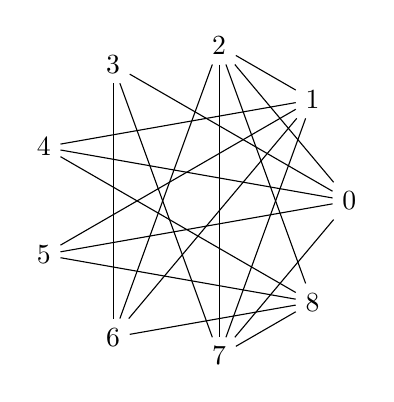
\begin{tikzpicture}
      \draw
        (0.0:2) node (0){0}
        (40.0:2) node (1){1}
        (80.0:2) node (2){2}
        (120.0:2) node (3){3}
        (160.0:2) node (4){4}
        (200.0:2) node (5){5}
        (240.0:2) node (6){6}
        (280.0:2) node (7){7}
        (320.0:2) node (8){8};
      \begin{scope}[-]
        \draw (0) to (2);
        \draw (0) to (3);
        \draw (0) to (4);
        \draw (0) to (5);
        \draw (0) to (7);
        \draw (1) to (2);
        \draw (1) to (4);
        \draw (1) to (5);
        \draw (1) to (6);
        \draw (1) to (7);
        \draw (2) to (6);
        \draw (2) to (7);
        \draw (2) to (8);
        \draw (3) to (6);
        \draw (3) to (7);
        \draw (4) to (8);
        \draw (5) to (8);
        \draw (6) to (8);
        \draw (7) to (8);
      \end{scope}
    \end{tikzpicture}
\end{figure}
\begin{itemize}
\item signature: 011110101011110000111001100001001011
\item g: Graph with 9 nodes and 19 edges
\item order: 9
\item size: 19
\item max degree: 5
\item degrees: 3,3,3,4,5,5,5,5,5
\item is tree: 0
\item is bipartite: 0
\item has bridge: 0
\item is chordal: 0
\item is complete: 0
\item min cycle basis weight: 38
\item min cycle basis size: 11
\item diameter: 2
\item radius: 2
\item is eulerian: 0
\item is planar: 0
\item number of faces: 12
\item is regular: 0
\item p3: 47
\item p4: None
\item property hash: fa13cb93ae203f7c694ec5c44bdc2863b3d399cd8517b36821574c985cd4c5de
\end{itemize}
\newpage
\begin{figure}
  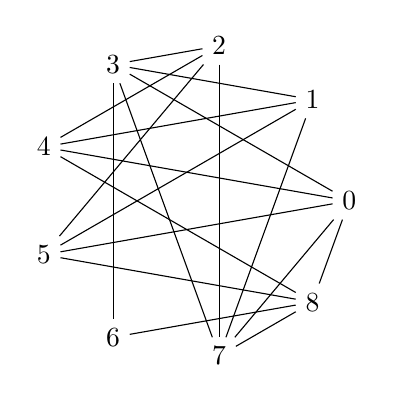
\begin{tikzpicture}
      \draw
        (0.0:2) node (0){0}
        (40.0:2) node (1){1}
        (80.0:2) node (2){2}
        (120.0:2) node (3){3}
        (160.0:2) node (4){4}
        (200.0:2) node (5){5}
        (240.0:2) node (6){6}
        (280.0:2) node (7){7}
        (320.0:2) node (8){8};
      \begin{scope}[-]
        \draw (0) to (3);
        \draw (0) to (4);
        \draw (0) to (5);
        \draw (0) to (7);
        \draw (0) to (8);
        \draw (1) to (3);
        \draw (1) to (4);
        \draw (1) to (5);
        \draw (1) to (7);
        \draw (2) to (3);
        \draw (2) to (4);
        \draw (2) to (5);
        \draw (2) to (7);
        \draw (3) to (6);
        \draw (3) to (7);
        \draw (4) to (8);
        \draw (5) to (8);
        \draw (6) to (8);
        \draw (7) to (8);
      \end{scope}
    \end{tikzpicture}
\end{figure}
\begin{itemize}
\item signature: 001110110111010111010001100001001011
\item g: Graph with 9 nodes and 19 edges
\item order: 9
\item size: 19
\item max degree: 5
\item degrees: 2,4,4,4,4,5,5,5,5
\item is tree: 0
\item is bipartite: 0
\item has bridge: 0
\item is chordal: 0
\item is complete: 0
\item min cycle basis weight: 38
\item min cycle basis size: 11
\item diameter: 2
\item radius: 2
\item is eulerian: 0
\item is planar: 0
\item number of faces: 12
\item is regular: 0
\item p3: 47
\item p4: None
\item property hash: d87df0ba57c2bd6afe881dc31971d83ab985980a49802f8f099b959d2cdbfe59
\end{itemize}
\newpage
\begin{figure}
  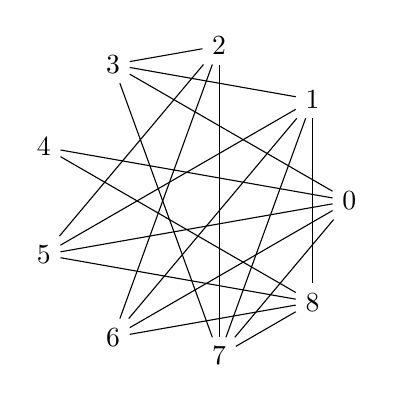
\begin{tikzpicture}
      \draw
        (0.0:2) node (0){0}
        (40.0:2) node (1){1}
        (80.0:2) node (2){2}
        (120.0:2) node (3){3}
        (160.0:2) node (4){4}
        (200.0:2) node (5){5}
        (240.0:2) node (6){6}
        (280.0:2) node (7){7}
        (320.0:2) node (8){8};
      \begin{scope}[-]
        \draw (0) to (3);
        \draw (0) to (4);
        \draw (0) to (5);
        \draw (0) to (6);
        \draw (0) to (7);
        \draw (1) to (3);
        \draw (1) to (5);
        \draw (1) to (6);
        \draw (1) to (7);
        \draw (1) to (8);
        \draw (2) to (3);
        \draw (2) to (5);
        \draw (2) to (6);
        \draw (2) to (7);
        \draw (3) to (7);
        \draw (4) to (8);
        \draw (5) to (8);
        \draw (6) to (8);
        \draw (7) to (8);
      \end{scope}
    \end{tikzpicture}
\end{figure}
\begin{itemize}
\item signature: 001111100101111101110000100001001011
\item g: Graph with 9 nodes and 19 edges
\item order: 9
\item size: 19
\item max degree: 5
\item degrees: 2,4,4,4,4,5,5,5,5
\item is tree: 0
\item is bipartite: 0
\item has bridge: 0
\item is chordal: 0
\item is complete: 0
\item min cycle basis weight: 38
\item min cycle basis size: 11
\item diameter: 3
\item radius: 2
\item is eulerian: 0
\item is planar: 0
\item number of faces: 12
\item is regular: 0
\item p3: 47
\item p4: 23
\item property hash: bedba4c9ee82e62c30c8ca79c4466e2ccac2f1c614781b2ffbd39fb8ccd63843
\end{itemize}
\newpage
\begin{figure}
  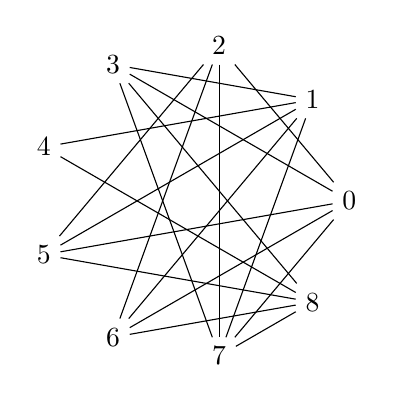
\begin{tikzpicture}
      \draw
        (0.0:2) node (0){0}
        (40.0:2) node (1){1}
        (80.0:2) node (2){2}
        (120.0:2) node (3){3}
        (160.0:2) node (4){4}
        (200.0:2) node (5){5}
        (240.0:2) node (6){6}
        (280.0:2) node (7){7}
        (320.0:2) node (8){8};
      \begin{scope}[-]
        \draw (0) to (2);
        \draw (0) to (3);
        \draw (0) to (5);
        \draw (0) to (6);
        \draw (0) to (7);
        \draw (1) to (3);
        \draw (1) to (4);
        \draw (1) to (5);
        \draw (1) to (6);
        \draw (1) to (7);
        \draw (2) to (5);
        \draw (2) to (6);
        \draw (2) to (7);
        \draw (3) to (7);
        \draw (3) to (8);
        \draw (4) to (8);
        \draw (5) to (8);
        \draw (6) to (8);
        \draw (7) to (8);
      \end{scope}
    \end{tikzpicture}
\end{figure}
\begin{itemize}
\item signature: 011011100111110001110000110001001011
\item g: Graph with 9 nodes and 19 edges
\item order: 9
\item size: 19
\item max degree: 5
\item degrees: 2,4,4,4,4,5,5,5,5
\item is tree: 0
\item is bipartite: 0
\item has bridge: 0
\item is chordal: 0
\item is complete: 0
\item min cycle basis weight: 38
\item min cycle basis size: 11
\item diameter: 3
\item radius: 2
\item is eulerian: 0
\item is planar: 0
\item number of faces: 12
\item is regular: 0
\item p3: 47
\item p4: 22
\item property hash: e24afc49f3c0c6fb80116903cd7d8c9a869acbfdcf49055840fa5663a2459e82
\end{itemize}
\newpage
\begin{figure}
  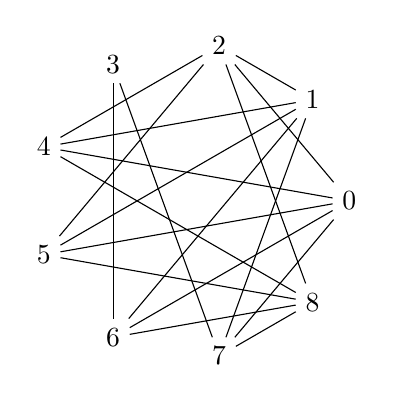
\begin{tikzpicture}
      \draw
        (0.0:2) node (0){0}
        (40.0:2) node (1){1}
        (80.0:2) node (2){2}
        (120.0:2) node (3){3}
        (160.0:2) node (4){4}
        (200.0:2) node (5){5}
        (240.0:2) node (6){6}
        (280.0:2) node (7){7}
        (320.0:2) node (8){8};
      \begin{scope}[-]
        \draw (0) to (2);
        \draw (0) to (4);
        \draw (0) to (5);
        \draw (0) to (6);
        \draw (0) to (7);
        \draw (1) to (2);
        \draw (1) to (4);
        \draw (1) to (5);
        \draw (1) to (6);
        \draw (1) to (7);
        \draw (2) to (4);
        \draw (2) to (5);
        \draw (2) to (8);
        \draw (3) to (6);
        \draw (3) to (7);
        \draw (4) to (8);
        \draw (5) to (8);
        \draw (6) to (8);
        \draw (7) to (8);
      \end{scope}
    \end{tikzpicture}
\end{figure}
\begin{itemize}
\item signature: 010111101011110011001001100001001011
\item g: Graph with 9 nodes and 19 edges
\item order: 9
\item size: 19
\item max degree: 5
\item degrees: 2,4,4,4,4,5,5,5,5
\item is tree: 0
\item is bipartite: 0
\item has bridge: 0
\item is chordal: 0
\item is complete: 0
\item min cycle basis weight: 38
\item min cycle basis size: 11
\item diameter: 3
\item radius: 2
\item is eulerian: 0
\item is planar: 0
\item number of faces: 12
\item is regular: 0
\item p3: 47
\item p4: None
\item property hash: 833307e133f41fd4d27e255a5cd4b3954357736a6959099cce4d5077ffcb8ecf
\end{itemize}
\newpage
\begin{figure}
  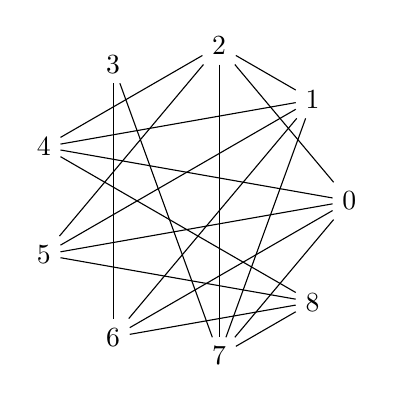
\begin{tikzpicture}
      \draw
        (0.0:2) node (0){0}
        (40.0:2) node (1){1}
        (80.0:2) node (2){2}
        (120.0:2) node (3){3}
        (160.0:2) node (4){4}
        (200.0:2) node (5){5}
        (240.0:2) node (6){6}
        (280.0:2) node (7){7}
        (320.0:2) node (8){8};
      \begin{scope}[-]
        \draw (0) to (2);
        \draw (0) to (4);
        \draw (0) to (5);
        \draw (0) to (6);
        \draw (0) to (7);
        \draw (1) to (2);
        \draw (1) to (4);
        \draw (1) to (5);
        \draw (1) to (6);
        \draw (1) to (7);
        \draw (2) to (4);
        \draw (2) to (5);
        \draw (2) to (7);
        \draw (3) to (6);
        \draw (3) to (7);
        \draw (4) to (8);
        \draw (5) to (8);
        \draw (6) to (8);
        \draw (7) to (8);
      \end{scope}
    \end{tikzpicture}
\end{figure}
\begin{itemize}
\item signature: 010111101011110011010001100001001011
\item g: Graph with 9 nodes and 19 edges
\item order: 9
\item size: 19
\item max degree: 5
\item degrees: 2,4,4,4,4,5,5,5,5
\item is tree: 0
\item is bipartite: 0
\item has bridge: 0
\item is chordal: 0
\item is complete: 0
\item min cycle basis weight: 38
\item min cycle basis size: 11
\item diameter: 3
\item radius: 2
\item is eulerian: 0
\item is planar: 0
\item number of faces: 12
\item is regular: 0
\item p3: 47
\item p4: 22
\item property hash: e24afc49f3c0c6fb80116903cd7d8c9a869acbfdcf49055840fa5663a2459e82
\end{itemize}
\newpage
\begin{figure}
  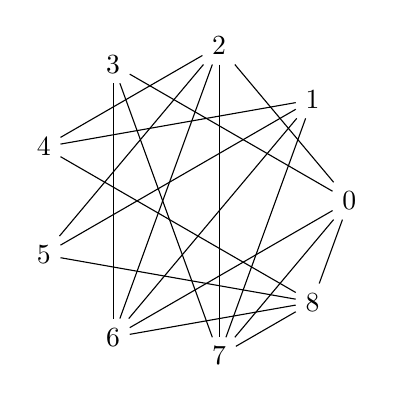
\begin{tikzpicture}
      \draw
        (0.0:2) node (0){0}
        (40.0:2) node (1){1}
        (80.0:2) node (2){2}
        (120.0:2) node (3){3}
        (160.0:2) node (4){4}
        (200.0:2) node (5){5}
        (240.0:2) node (6){6}
        (280.0:2) node (7){7}
        (320.0:2) node (8){8};
      \begin{scope}[-]
        \draw (0) to (2);
        \draw (0) to (3);
        \draw (0) to (6);
        \draw (0) to (7);
        \draw (0) to (8);
        \draw (1) to (4);
        \draw (1) to (5);
        \draw (1) to (6);
        \draw (1) to (7);
        \draw (2) to (4);
        \draw (2) to (5);
        \draw (2) to (6);
        \draw (2) to (7);
        \draw (3) to (6);
        \draw (3) to (7);
        \draw (4) to (8);
        \draw (5) to (8);
        \draw (6) to (8);
        \draw (7) to (8);
      \end{scope}
    \end{tikzpicture}
\end{figure}
\begin{itemize}
\item signature: 011001110011110011110001100001001011
\item g: Graph with 9 nodes and 19 edges
\item order: 9
\item size: 19
\item max degree: 5
\item degrees: 3,3,3,4,5,5,5,5,5
\item is tree: 0
\item is bipartite: 0
\item has bridge: 0
\item is chordal: 0
\item is complete: 0
\item min cycle basis weight: 38
\item min cycle basis size: 11
\item diameter: 3
\item radius: 2
\item is eulerian: 0
\item is planar: 0
\item number of faces: 12
\item is regular: 0
\item p3: 47
\item p4: 24
\item property hash: a3d568faf8cf876899a2e9b2ce99d63ec7a4d881ceb80841dc381702bad0a17a
\end{itemize}
\newpage
\begin{figure}
  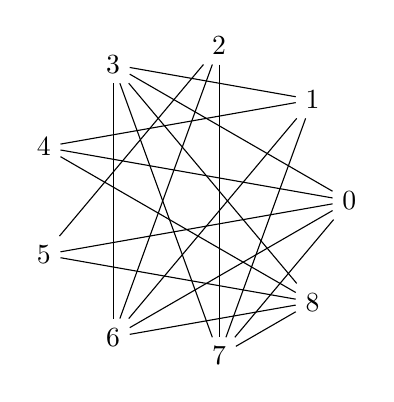
\begin{tikzpicture}
      \draw
        (0.0:2) node (0){0}
        (40.0:2) node (1){1}
        (80.0:2) node (2){2}
        (120.0:2) node (3){3}
        (160.0:2) node (4){4}
        (200.0:2) node (5){5}
        (240.0:2) node (6){6}
        (280.0:2) node (7){7}
        (320.0:2) node (8){8};
      \begin{scope}[-]
        \draw (0) to (3);
        \draw (0) to (4);
        \draw (0) to (5);
        \draw (0) to (6);
        \draw (0) to (7);
        \draw (1) to (3);
        \draw (1) to (4);
        \draw (1) to (6);
        \draw (1) to (7);
        \draw (2) to (5);
        \draw (2) to (6);
        \draw (2) to (7);
        \draw (3) to (6);
        \draw (3) to (7);
        \draw (3) to (8);
        \draw (4) to (8);
        \draw (5) to (8);
        \draw (6) to (8);
        \draw (7) to (8);
      \end{scope}
    \end{tikzpicture}
\end{figure}
\begin{itemize}
\item signature: 001111100110110001110001110001001011
\item g: Graph with 9 nodes and 19 edges
\item order: 9
\item size: 19
\item max degree: 5
\item degrees: 3,3,3,4,5,5,5,5,5
\item is tree: 0
\item is bipartite: 0
\item has bridge: 0
\item is chordal: 0
\item is complete: 0
\item min cycle basis weight: 38
\item min cycle basis size: 11
\item diameter: 3
\item radius: 2
\item is eulerian: 0
\item is planar: 0
\item number of faces: 12
\item is regular: 0
\item p3: 47
\item p4: 22
\item property hash: 3395c5ef99f0317480f3348717c6e4f82d36f5e3de35324b6f22f68d5fc62085
\end{itemize}
\newpage
\begin{figure}
  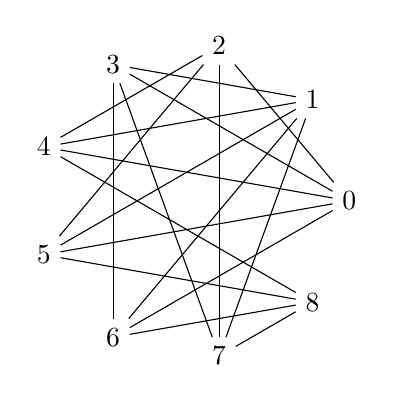
\begin{tikzpicture}
      \draw
        (0.0:2) node (0){0}
        (40.0:2) node (1){1}
        (80.0:2) node (2){2}
        (120.0:2) node (3){3}
        (160.0:2) node (4){4}
        (200.0:2) node (5){5}
        (240.0:2) node (6){6}
        (280.0:2) node (7){7}
        (320.0:2) node (8){8};
      \begin{scope}[-]
        \draw (0) to (2);
        \draw (0) to (3);
        \draw (0) to (4);
        \draw (0) to (5);
        \draw (0) to (6);
        \draw (1) to (3);
        \draw (1) to (4);
        \draw (1) to (5);
        \draw (1) to (6);
        \draw (1) to (7);
        \draw (2) to (4);
        \draw (2) to (5);
        \draw (2) to (7);
        \draw (3) to (6);
        \draw (3) to (7);
        \draw (4) to (8);
        \draw (5) to (8);
        \draw (6) to (8);
        \draw (7) to (8);
      \end{scope}
    \end{tikzpicture}
\end{figure}
\begin{itemize}
\item signature: 011111000111110011010001100001001011
\item g: Graph with 9 nodes and 19 edges
\item order: 9
\item size: 19
\item max degree: 5
\item degrees: 4,4,4,4,4,4,4,5,5
\item is tree: 0
\item is bipartite: 0
\item has bridge: 0
\item is chordal: 0
\item is complete: 0
\item min cycle basis weight: 39
\item min cycle basis size: 11
\item diameter: 2
\item radius: 2
\item is eulerian: 0
\item is planar: 0
\item number of faces: 12
\item is regular: 0
\item p3: 47
\item p4: 34
\item property hash: d66c3506d4daae8c5b8c0d5d8eefe0492ba5a574c684041f0417b9018f943b33
\end{itemize}
\newpage
\begin{figure}
  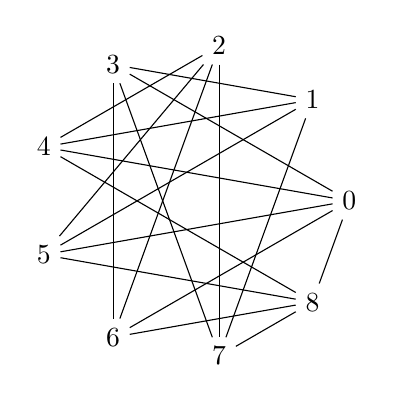
\begin{tikzpicture}
      \draw
        (0.0:2) node (0){0}
        (40.0:2) node (1){1}
        (80.0:2) node (2){2}
        (120.0:2) node (3){3}
        (160.0:2) node (4){4}
        (200.0:2) node (5){5}
        (240.0:2) node (6){6}
        (280.0:2) node (7){7}
        (320.0:2) node (8){8};
      \begin{scope}[-]
        \draw (0) to (3);
        \draw (0) to (4);
        \draw (0) to (5);
        \draw (0) to (6);
        \draw (0) to (8);
        \draw (1) to (3);
        \draw (1) to (4);
        \draw (1) to (5);
        \draw (1) to (7);
        \draw (2) to (4);
        \draw (2) to (5);
        \draw (2) to (6);
        \draw (2) to (7);
        \draw (3) to (6);
        \draw (3) to (7);
        \draw (4) to (8);
        \draw (5) to (8);
        \draw (6) to (8);
        \draw (7) to (8);
      \end{scope}
    \end{tikzpicture}
\end{figure}
\begin{itemize}
\item signature: 001111010111010011110001100001001011
\item g: Graph with 9 nodes and 19 edges
\item order: 9
\item size: 19
\item max degree: 5
\item degrees: 4,4,4,4,4,4,4,5,5
\item is tree: 0
\item is bipartite: 0
\item has bridge: 0
\item is chordal: 0
\item is complete: 0
\item min cycle basis weight: 39
\item min cycle basis size: 11
\item diameter: 2
\item radius: 2
\item is eulerian: 0
\item is planar: 0
\item number of faces: 12
\item is regular: 0
\item p3: 47
\item p4: 37
\item property hash: e9365ea869b8dec0dc41177d61b80832eeeaf817c85956281cd965182b356879
\end{itemize}
\newpage
\begin{figure}
  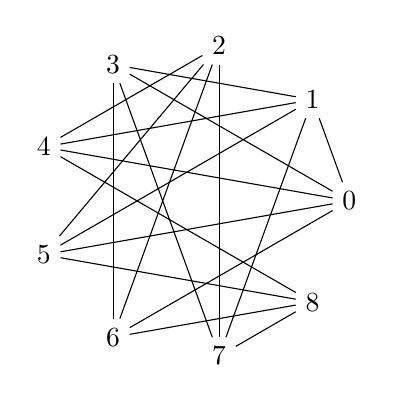
\begin{tikzpicture}
      \draw
        (0.0:2) node (0){0}
        (40.0:2) node (1){1}
        (80.0:2) node (2){2}
        (120.0:2) node (3){3}
        (160.0:2) node (4){4}
        (200.0:2) node (5){5}
        (240.0:2) node (6){6}
        (280.0:2) node (7){7}
        (320.0:2) node (8){8};
      \begin{scope}[-]
        \draw (0) to (1);
        \draw (0) to (3);
        \draw (0) to (4);
        \draw (0) to (5);
        \draw (0) to (6);
        \draw (1) to (3);
        \draw (1) to (4);
        \draw (1) to (5);
        \draw (1) to (7);
        \draw (2) to (4);
        \draw (2) to (5);
        \draw (2) to (6);
        \draw (2) to (7);
        \draw (3) to (6);
        \draw (3) to (7);
        \draw (4) to (8);
        \draw (5) to (8);
        \draw (6) to (8);
        \draw (7) to (8);
      \end{scope}
    \end{tikzpicture}
\end{figure}
\begin{itemize}
\item signature: 101111000111010011110001100001001011
\item g: Graph with 9 nodes and 19 edges
\item order: 9
\item size: 19
\item max degree: 5
\item degrees: 4,4,4,4,4,4,4,5,5
\item is tree: 0
\item is bipartite: 0
\item has bridge: 0
\item is chordal: 0
\item is complete: 0
\item min cycle basis weight: 39
\item min cycle basis size: 11
\item diameter: 2
\item radius: 2
\item is eulerian: 0
\item is planar: 0
\item number of faces: 12
\item is regular: 0
\item p3: 47
\item p4: 41
\item property hash: 4e8d190129f964f6d968b6117eb1503a28a5735fcba5afff93b6b302bfec5e32
\end{itemize}
\newpage
\begin{figure}
  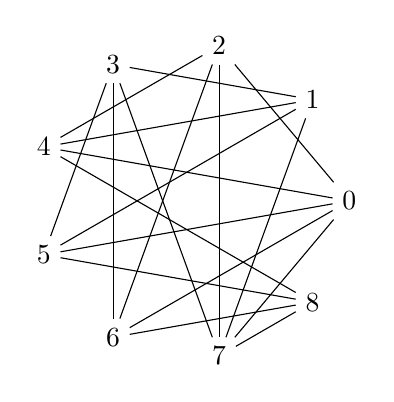
\begin{tikzpicture}
      \draw
        (0.0:2) node (0){0}
        (40.0:2) node (1){1}
        (80.0:2) node (2){2}
        (120.0:2) node (3){3}
        (160.0:2) node (4){4}
        (200.0:2) node (5){5}
        (240.0:2) node (6){6}
        (280.0:2) node (7){7}
        (320.0:2) node (8){8};
      \begin{scope}[-]
        \draw (0) to (2);
        \draw (0) to (4);
        \draw (0) to (5);
        \draw (0) to (6);
        \draw (0) to (7);
        \draw (1) to (3);
        \draw (1) to (4);
        \draw (1) to (5);
        \draw (1) to (7);
        \draw (2) to (4);
        \draw (2) to (6);
        \draw (2) to (7);
        \draw (3) to (5);
        \draw (3) to (6);
        \draw (3) to (7);
        \draw (4) to (8);
        \draw (5) to (8);
        \draw (6) to (8);
        \draw (7) to (8);
      \end{scope}
    \end{tikzpicture}
\end{figure}
\begin{itemize}
\item signature: 010111100111010010110011100001001011
\item g: Graph with 9 nodes and 19 edges
\item order: 9
\item size: 19
\item max degree: 5
\item degrees: 4,4,4,4,4,4,4,5,5
\item is tree: 0
\item is bipartite: 0
\item has bridge: 0
\item is chordal: 0
\item is complete: 0
\item min cycle basis weight: 39
\item min cycle basis size: 11
\item diameter: 2
\item radius: 2
\item is eulerian: 0
\item is planar: 0
\item number of faces: 12
\item is regular: 0
\item p3: 47
\item p4: 33
\item property hash: cf2252f95f30ff8b54d109a2af2120e87105c959ce395d6da0d14017bbd367bf
\end{itemize}
\newpage
\begin{figure}
  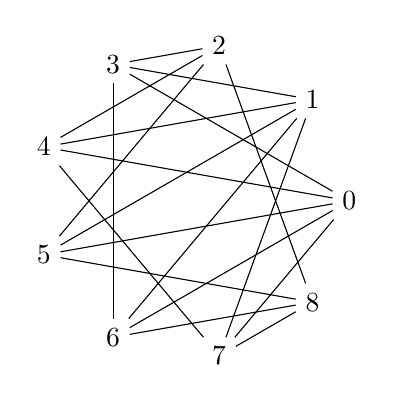
\begin{tikzpicture}
      \draw
        (0.0:2) node (0){0}
        (40.0:2) node (1){1}
        (80.0:2) node (2){2}
        (120.0:2) node (3){3}
        (160.0:2) node (4){4}
        (200.0:2) node (5){5}
        (240.0:2) node (6){6}
        (280.0:2) node (7){7}
        (320.0:2) node (8){8};
      \begin{scope}[-]
        \draw (0) to (3);
        \draw (0) to (4);
        \draw (0) to (5);
        \draw (0) to (6);
        \draw (0) to (7);
        \draw (1) to (3);
        \draw (1) to (4);
        \draw (1) to (5);
        \draw (1) to (6);
        \draw (1) to (7);
        \draw (2) to (3);
        \draw (2) to (4);
        \draw (2) to (5);
        \draw (2) to (8);
        \draw (3) to (6);
        \draw (4) to (7);
        \draw (5) to (8);
        \draw (6) to (8);
        \draw (7) to (8);
      \end{scope}
    \end{tikzpicture}
\end{figure}
\begin{itemize}
\item signature: 001111100111110111001001000010001011
\item g: Graph with 9 nodes and 19 edges
\item order: 9
\item size: 19
\item max degree: 5
\item degrees: 4,4,4,4,4,4,4,5,5
\item is tree: 0
\item is bipartite: 0
\item has bridge: 0
\item is chordal: 0
\item is complete: 0
\item min cycle basis weight: 39
\item min cycle basis size: 11
\item diameter: 2
\item radius: 2
\item is eulerian: 0
\item is planar: 0
\item number of faces: 12
\item is regular: 0
\item p3: 47
\item p4: 34
\item property hash: d66c3506d4daae8c5b8c0d5d8eefe0492ba5a574c684041f0417b9018f943b33
\end{itemize}
\newpage
\begin{figure}
  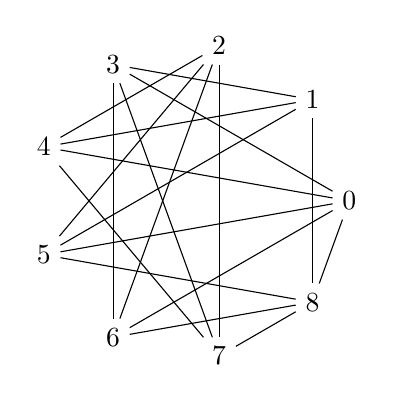
\begin{tikzpicture}
      \draw
        (0.0:2) node (0){0}
        (40.0:2) node (1){1}
        (80.0:2) node (2){2}
        (120.0:2) node (3){3}
        (160.0:2) node (4){4}
        (200.0:2) node (5){5}
        (240.0:2) node (6){6}
        (280.0:2) node (7){7}
        (320.0:2) node (8){8};
      \begin{scope}[-]
        \draw (0) to (3);
        \draw (0) to (4);
        \draw (0) to (5);
        \draw (0) to (6);
        \draw (0) to (8);
        \draw (1) to (3);
        \draw (1) to (4);
        \draw (1) to (5);
        \draw (1) to (8);
        \draw (2) to (4);
        \draw (2) to (5);
        \draw (2) to (6);
        \draw (2) to (7);
        \draw (3) to (6);
        \draw (3) to (7);
        \draw (4) to (7);
        \draw (5) to (8);
        \draw (6) to (8);
        \draw (7) to (8);
      \end{scope}
    \end{tikzpicture}
\end{figure}
\begin{itemize}
\item signature: 001111010111001011110001100010001011
\item g: Graph with 9 nodes and 19 edges
\item order: 9
\item size: 19
\item max degree: 5
\item degrees: 4,4,4,4,4,4,4,5,5
\item is tree: 0
\item is bipartite: 0
\item has bridge: 0
\item is chordal: 0
\item is complete: 0
\item min cycle basis weight: 39
\item min cycle basis size: 11
\item diameter: 2
\item radius: 2
\item is eulerian: 0
\item is planar: 0
\item number of faces: 12
\item is regular: 0
\item p3: 47
\item p4: 37
\item property hash: e9365ea869b8dec0dc41177d61b80832eeeaf817c85956281cd965182b356879
\end{itemize}
\newpage
\begin{figure}
  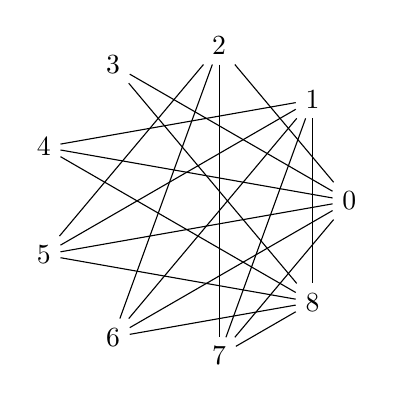
\begin{tikzpicture}
      \draw
        (0.0:2) node (0){0}
        (40.0:2) node (1){1}
        (80.0:2) node (2){2}
        (120.0:2) node (3){3}
        (160.0:2) node (4){4}
        (200.0:2) node (5){5}
        (240.0:2) node (6){6}
        (280.0:2) node (7){7}
        (320.0:2) node (8){8};
      \begin{scope}[-]
        \draw (0) to (2);
        \draw (0) to (3);
        \draw (0) to (4);
        \draw (0) to (5);
        \draw (0) to (6);
        \draw (0) to (7);
        \draw (1) to (4);
        \draw (1) to (5);
        \draw (1) to (6);
        \draw (1) to (7);
        \draw (1) to (8);
        \draw (2) to (5);
        \draw (2) to (6);
        \draw (2) to (7);
        \draw (3) to (8);
        \draw (4) to (8);
        \draw (5) to (8);
        \draw (6) to (8);
        \draw (7) to (8);
      \end{scope}
    \end{tikzpicture}
\end{figure}
\begin{itemize}
\item signature: 011111100011111001110000010001001011
\item g: Graph with 9 nodes and 19 edges
\item order: 9
\item size: 19
\item max degree: 6
\item degrees: 2,3,4,4,4,4,5,6,6
\item is tree: 0
\item is bipartite: 0
\item has bridge: 0
\item is chordal: 0
\item is complete: 0
\item min cycle basis weight: 37
\item min cycle basis size: 11
\item diameter: 2
\item radius: 2
\item is eulerian: 0
\item is planar: 0
\item number of faces: 12
\item is regular: 0
\item p3: 47
\item p4: 17
\item property hash: 589fdaf33e85bb13c9c341a8cb36e7fd50adca134469965322183b7b82ce7f97
\end{itemize}
\newpage
\begin{figure}
  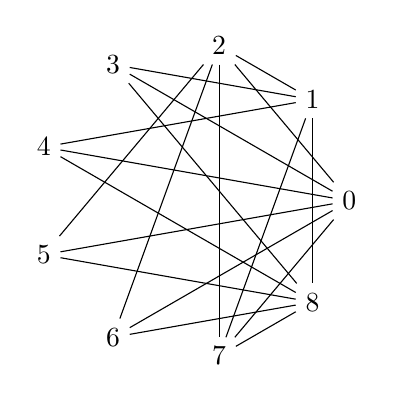
\begin{tikzpicture}
      \draw
        (0.0:2) node (0){0}
        (40.0:2) node (1){1}
        (80.0:2) node (2){2}
        (120.0:2) node (3){3}
        (160.0:2) node (4){4}
        (200.0:2) node (5){5}
        (240.0:2) node (6){6}
        (280.0:2) node (7){7}
        (320.0:2) node (8){8};
      \begin{scope}[-]
        \draw (0) to (2);
        \draw (0) to (3);
        \draw (0) to (4);
        \draw (0) to (5);
        \draw (0) to (6);
        \draw (0) to (7);
        \draw (1) to (2);
        \draw (1) to (3);
        \draw (1) to (4);
        \draw (1) to (7);
        \draw (1) to (8);
        \draw (2) to (5);
        \draw (2) to (6);
        \draw (2) to (7);
        \draw (3) to (8);
        \draw (4) to (8);
        \draw (5) to (8);
        \draw (6) to (8);
        \draw (7) to (8);
      \end{scope}
    \end{tikzpicture}
\end{figure}
\begin{itemize}
\item signature: 011111101110011001110000010001001011
\item g: Graph with 9 nodes and 19 edges
\item order: 9
\item size: 19
\item max degree: 6
\item degrees: 3,3,3,3,4,5,5,6,6
\item is tree: 0
\item is bipartite: 0
\item has bridge: 0
\item is chordal: 0
\item is complete: 0
\item min cycle basis weight: 37
\item min cycle basis size: 11
\item diameter: 2
\item radius: 2
\item is eulerian: 0
\item is planar: 0
\item number of faces: 12
\item is regular: 0
\item p3: 47
\item p4: 21
\item property hash: ea1fe2db767f4f4d37bea7678c585711723ee285a67aca28e98989b79b89e990
\end{itemize}
\newpage
\begin{figure}
  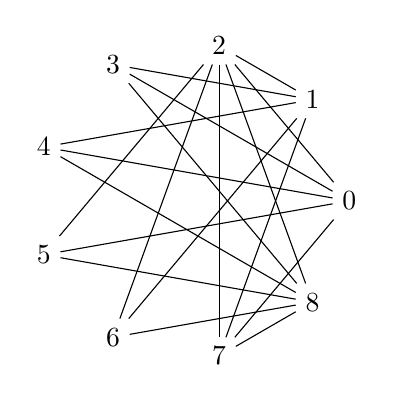
\begin{tikzpicture}
      \draw
        (0.0:2) node (0){0}
        (40.0:2) node (1){1}
        (80.0:2) node (2){2}
        (120.0:2) node (3){3}
        (160.0:2) node (4){4}
        (200.0:2) node (5){5}
        (240.0:2) node (6){6}
        (280.0:2) node (7){7}
        (320.0:2) node (8){8};
      \begin{scope}[-]
        \draw (0) to (2);
        \draw (0) to (3);
        \draw (0) to (4);
        \draw (0) to (5);
        \draw (0) to (7);
        \draw (1) to (2);
        \draw (1) to (3);
        \draw (1) to (4);
        \draw (1) to (6);
        \draw (1) to (7);
        \draw (2) to (5);
        \draw (2) to (6);
        \draw (2) to (7);
        \draw (2) to (8);
        \draw (3) to (8);
        \draw (4) to (8);
        \draw (5) to (8);
        \draw (6) to (8);
        \draw (7) to (8);
      \end{scope}
    \end{tikzpicture}
\end{figure}
\begin{itemize}
\item signature: 011110101110110001111000010001001011
\item g: Graph with 9 nodes and 19 edges
\item order: 9
\item size: 19
\item max degree: 6
\item degrees: 3,3,3,3,4,5,5,6,6
\item is tree: 0
\item is bipartite: 0
\item has bridge: 0
\item is chordal: 0
\item is complete: 0
\item min cycle basis weight: 37
\item min cycle basis size: 11
\item diameter: 2
\item radius: 2
\item is eulerian: 0
\item is planar: 0
\item number of faces: 12
\item is regular: 0
\item p3: 47
\item p4: None
\item property hash: 8128fc051ebd823d65c8aee3d479665378f423680a118746da37342c5db0d6f7
\end{itemize}
\newpage
\begin{figure}
  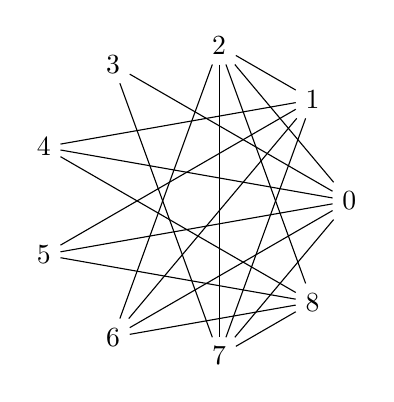
\begin{tikzpicture}
      \draw
        (0.0:2) node (0){0}
        (40.0:2) node (1){1}
        (80.0:2) node (2){2}
        (120.0:2) node (3){3}
        (160.0:2) node (4){4}
        (200.0:2) node (5){5}
        (240.0:2) node (6){6}
        (280.0:2) node (7){7}
        (320.0:2) node (8){8};
      \begin{scope}[-]
        \draw (0) to (2);
        \draw (0) to (3);
        \draw (0) to (4);
        \draw (0) to (5);
        \draw (0) to (6);
        \draw (0) to (7);
        \draw (1) to (2);
        \draw (1) to (4);
        \draw (1) to (5);
        \draw (1) to (6);
        \draw (1) to (7);
        \draw (2) to (6);
        \draw (2) to (7);
        \draw (2) to (8);
        \draw (3) to (7);
        \draw (4) to (8);
        \draw (5) to (8);
        \draw (6) to (8);
        \draw (7) to (8);
      \end{scope}
    \end{tikzpicture}
\end{figure}
\begin{itemize}
\item signature: 011111101011110000111000100001001011
\item g: Graph with 9 nodes and 19 edges
\item order: 9
\item size: 19
\item max degree: 6
\item degrees: 2,3,3,4,5,5,5,5,6
\item is tree: 0
\item is bipartite: 0
\item has bridge: 0
\item is chordal: 0
\item is complete: 0
\item min cycle basis weight: 37
\item min cycle basis size: 11
\item diameter: 2
\item radius: 2
\item is eulerian: 0
\item is planar: 0
\item number of faces: 12
\item is regular: 0
\item p3: 47
\item p4: None
\item property hash: a956930c3ff3ff893735df6959b0d81d4a14d33686c643784e4123cd7529dcea
\end{itemize}
\newpage
\begin{figure}
  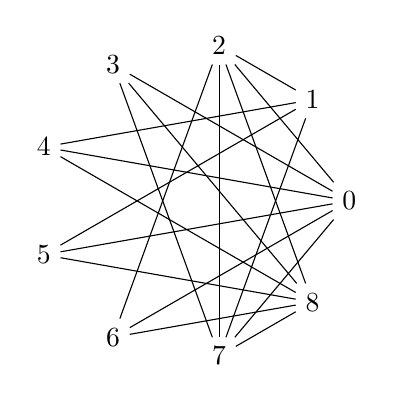
\begin{tikzpicture}
      \draw
        (0.0:2) node (0){0}
        (40.0:2) node (1){1}
        (80.0:2) node (2){2}
        (120.0:2) node (3){3}
        (160.0:2) node (4){4}
        (200.0:2) node (5){5}
        (240.0:2) node (6){6}
        (280.0:2) node (7){7}
        (320.0:2) node (8){8};
      \begin{scope}[-]
        \draw (0) to (2);
        \draw (0) to (3);
        \draw (0) to (4);
        \draw (0) to (5);
        \draw (0) to (6);
        \draw (0) to (7);
        \draw (1) to (2);
        \draw (1) to (4);
        \draw (1) to (5);
        \draw (1) to (7);
        \draw (2) to (6);
        \draw (2) to (7);
        \draw (2) to (8);
        \draw (3) to (7);
        \draw (3) to (8);
        \draw (4) to (8);
        \draw (5) to (8);
        \draw (6) to (8);
        \draw (7) to (8);
      \end{scope}
    \end{tikzpicture}
\end{figure}
\begin{itemize}
\item signature: 011111101011010000111000110001001011
\item g: Graph with 9 nodes and 19 edges
\item order: 9
\item size: 19
\item max degree: 6
\item degrees: 3,3,3,3,4,5,5,6,6
\item is tree: 0
\item is bipartite: 0
\item has bridge: 0
\item is chordal: 0
\item is complete: 0
\item min cycle basis weight: 37
\item min cycle basis size: 11
\item diameter: 2
\item radius: 2
\item is eulerian: 0
\item is planar: 0
\item number of faces: 12
\item is regular: 0
\item p3: 47
\item p4: 17
\item property hash: b8d5fb9cfea36e1a2ac7f46a31f63c8ff335ca4dfa2c0e94d0764d56f5e19ad4
\end{itemize}
\newpage
\begin{figure}
  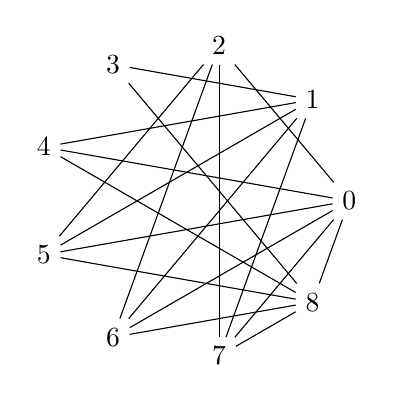
\begin{tikzpicture}
      \draw
        (0.0:2) node (0){0}
        (40.0:2) node (1){1}
        (80.0:2) node (2){2}
        (120.0:2) node (3){3}
        (160.0:2) node (4){4}
        (200.0:2) node (5){5}
        (240.0:2) node (6){6}
        (280.0:2) node (7){7}
        (320.0:2) node (8){8};
      \begin{scope}[-]
        \draw (0) to (2);
        \draw (0) to (4);
        \draw (0) to (5);
        \draw (0) to (6);
        \draw (0) to (7);
        \draw (0) to (8);
        \draw (1) to (3);
        \draw (1) to (4);
        \draw (1) to (5);
        \draw (1) to (6);
        \draw (1) to (7);
        \draw (2) to (5);
        \draw (2) to (6);
        \draw (2) to (7);
        \draw (3) to (8);
        \draw (4) to (8);
        \draw (5) to (8);
        \draw (6) to (8);
        \draw (7) to (8);
      \end{scope}
    \end{tikzpicture}
\end{figure}
\begin{itemize}
\item signature: 010111110111110001110000010001001011
\item g: Graph with 9 nodes and 19 edges
\item order: 9
\item size: 19
\item max degree: 6
\item degrees: 2,3,4,4,4,4,5,6,6
\item is tree: 0
\item is bipartite: 0
\item has bridge: 0
\item is chordal: 0
\item is complete: 0
\item min cycle basis weight: 37
\item min cycle basis size: 11
\item diameter: 3
\item radius: 2
\item is eulerian: 0
\item is planar: 0
\item number of faces: 12
\item is regular: 0
\item p3: 47
\item p4: 19
\item property hash: 8469b31e9fcaacde430a996ecc14df50247c66a3b7c1a767f4c055fd5c041532
\end{itemize}
\newpage
\begin{figure}
  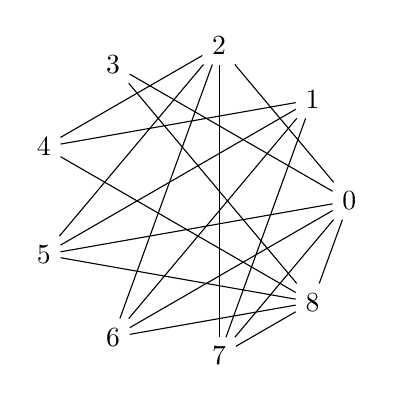
\begin{tikzpicture}
      \draw
        (0.0:2) node (0){0}
        (40.0:2) node (1){1}
        (80.0:2) node (2){2}
        (120.0:2) node (3){3}
        (160.0:2) node (4){4}
        (200.0:2) node (5){5}
        (240.0:2) node (6){6}
        (280.0:2) node (7){7}
        (320.0:2) node (8){8};
      \begin{scope}[-]
        \draw (0) to (2);
        \draw (0) to (3);
        \draw (0) to (5);
        \draw (0) to (6);
        \draw (0) to (7);
        \draw (0) to (8);
        \draw (1) to (4);
        \draw (1) to (5);
        \draw (1) to (6);
        \draw (1) to (7);
        \draw (2) to (4);
        \draw (2) to (5);
        \draw (2) to (6);
        \draw (2) to (7);
        \draw (3) to (8);
        \draw (4) to (8);
        \draw (5) to (8);
        \draw (6) to (8);
        \draw (7) to (8);
      \end{scope}
    \end{tikzpicture}
\end{figure}
\begin{itemize}
\item signature: 011011110011110011110000010001001011
\item g: Graph with 9 nodes and 19 edges
\item order: 9
\item size: 19
\item max degree: 6
\item degrees: 2,3,4,4,4,4,5,6,6
\item is tree: 0
\item is bipartite: 0
\item has bridge: 0
\item is chordal: 0
\item is complete: 0
\item min cycle basis weight: 37
\item min cycle basis size: 11
\item diameter: 3
\item radius: 2
\item is eulerian: 0
\item is planar: 0
\item number of faces: 12
\item is regular: 0
\item p3: 47
\item p4: 17
\item property hash: ce9746fc9c545c541e9b3d84b3b6fc2310f4bf755d737ba48c3375eb2e0e3e25
\end{itemize}
\newpage
\begin{figure}
  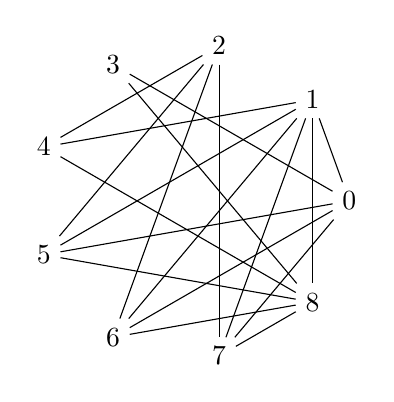
\begin{tikzpicture}
      \draw
        (0.0:2) node (0){0}
        (40.0:2) node (1){1}
        (80.0:2) node (2){2}
        (120.0:2) node (3){3}
        (160.0:2) node (4){4}
        (200.0:2) node (5){5}
        (240.0:2) node (6){6}
        (280.0:2) node (7){7}
        (320.0:2) node (8){8};
      \begin{scope}[-]
        \draw (0) to (1);
        \draw (0) to (3);
        \draw (0) to (5);
        \draw (0) to (6);
        \draw (0) to (7);
        \draw (1) to (4);
        \draw (1) to (5);
        \draw (1) to (6);
        \draw (1) to (7);
        \draw (1) to (8);
        \draw (2) to (4);
        \draw (2) to (5);
        \draw (2) to (6);
        \draw (2) to (7);
        \draw (3) to (8);
        \draw (4) to (8);
        \draw (5) to (8);
        \draw (6) to (8);
        \draw (7) to (8);
      \end{scope}
    \end{tikzpicture}
\end{figure}
\begin{itemize}
\item signature: 101011100011111011110000010001001011
\item g: Graph with 9 nodes and 19 edges
\item order: 9
\item size: 19
\item max degree: 6
\item degrees: 2,3,4,4,4,4,5,6,6
\item is tree: 0
\item is bipartite: 0
\item has bridge: 0
\item is chordal: 0
\item is complete: 0
\item min cycle basis weight: 37
\item min cycle basis size: 11
\item diameter: 3
\item radius: 2
\item is eulerian: 0
\item is planar: 0
\item number of faces: 12
\item is regular: 0
\item p3: 47
\item p4: None
\item property hash: e22f7d494c480b5510152a8639d14e94ce5e1920bcf0cf37460dfb3e9dcc54c2
\end{itemize}
\newpage
\begin{figure}
  \begin{tikzpicture}
      \draw
        (0.0:2) node (0){0}
        (40.0:2) node (1){1}
        (80.0:2) node (2){2}
        (120.0:2) node (3){3}
        (160.0:2) node (4){4}
        (200.0:2) node (5){5}
        (240.0:2) node (6){6}
        (280.0:2) node (7){7}
        (320.0:2) node (8){8};
      \begin{scope}[-]
        \draw (0) to (1);
        \draw (0) to (2);
        \draw (0) to (3);
        \draw (0) to (6);
        \draw (0) to (7);
        \draw (0) to (8);
        \draw (1) to (4);
        \draw (1) to (5);
        \draw (1) to (6);
        \draw (1) to (7);
        \draw (2) to (4);
        \draw (2) to (5);
        \draw (2) to (6);
        \draw (2) to (7);
        \draw (3) to (7);
        \draw (4) to (8);
        \draw (5) to (8);
        \draw (6) to (8);
        \draw (7) to (8);
      \end{scope}
    \end{tikzpicture}
\end{figure}
\begin{itemize}
\item signature: 111001110011110011110000100001001011
\item g: Graph with 9 nodes and 19 edges
\item order: 9
\item size: 19
\item max degree: 6
\item degrees: 2,3,3,4,5,5,5,5,6
\item is tree: 0
\item is bipartite: 0
\item has bridge: 0
\item is chordal: 0
\item is complete: 0
\item min cycle basis weight: 37
\item min cycle basis size: 11
\item diameter: 3
\item radius: 2
\item is eulerian: 0
\item is planar: 0
\item number of faces: 12
\item is regular: 0
\item p3: 47
\item p4: None
\item property hash: 921bc2dee1d88f74c3ec9b4d7c34fc8cdbebbfa223e8faca78a8714ebed5f436
\end{itemize}
\newpage
\begin{figure}
  \begin{tikzpicture}
      \draw
        (0.0:2) node (0){0}
        (40.0:2) node (1){1}
        (80.0:2) node (2){2}
        (120.0:2) node (3){3}
        (160.0:2) node (4){4}
        (200.0:2) node (5){5}
        (240.0:2) node (6){6}
        (280.0:2) node (7){7}
        (320.0:2) node (8){8};
      \begin{scope}[-]
        \draw (0) to (2);
        \draw (0) to (3);
        \draw (0) to (4);
        \draw (0) to (5);
        \draw (0) to (6);
        \draw (0) to (7);
        \draw (1) to (3);
        \draw (1) to (5);
        \draw (1) to (6);
        \draw (1) to (7);
        \draw (2) to (6);
        \draw (2) to (7);
        \draw (2) to (8);
        \draw (3) to (7);
        \draw (3) to (8);
        \draw (4) to (8);
        \draw (5) to (8);
        \draw (6) to (8);
        \draw (7) to (8);
      \end{scope}
    \end{tikzpicture}
\end{figure}
\begin{itemize}
\item signature: 011111100101110000111000110001001011
\item g: Graph with 9 nodes and 19 edges
\item order: 9
\item size: 19
\item max degree: 6
\item degrees: 2,3,4,4,4,4,5,6,6
\item is tree: 0
\item is bipartite: 0
\item has bridge: 0
\item is chordal: 0
\item is complete: 0
\item min cycle basis weight: 37
\item min cycle basis size: 11
\item diameter: 3
\item radius: 2
\item is eulerian: 0
\item is planar: 0
\item number of faces: 12
\item is regular: 0
\item p3: 47
\item p4: 16
\item property hash: 661e91cca4b3a96cbd288a0e9fc4faf692f0f3a8ef0fe26498a75e1237a4e9c6
\end{itemize}
\newpage
\begin{figure}
  \begin{tikzpicture}
      \draw
        (0.0:2) node (0){0}
        (40.0:2) node (1){1}
        (80.0:2) node (2){2}
        (120.0:2) node (3){3}
        (160.0:2) node (4){4}
        (200.0:2) node (5){5}
        (240.0:2) node (6){6}
        (280.0:2) node (7){7}
        (320.0:2) node (8){8};
      \begin{scope}[-]
        \draw (0) to (2);
        \draw (0) to (3);
        \draw (0) to (4);
        \draw (0) to (5);
        \draw (0) to (6);
        \draw (0) to (7);
        \draw (1) to (3);
        \draw (1) to (4);
        \draw (1) to (5);
        \draw (1) to (6);
        \draw (1) to (7);
        \draw (2) to (5);
        \draw (2) to (6);
        \draw (2) to (8);
        \draw (3) to (7);
        \draw (4) to (8);
        \draw (5) to (8);
        \draw (6) to (8);
        \draw (7) to (8);
      \end{scope}
    \end{tikzpicture}
\end{figure}
\begin{itemize}
\item signature: 011111100111110001101000100001001011
\item g: Graph with 9 nodes and 19 edges
\item order: 9
\item size: 19
\item max degree: 6
\item degrees: 3,3,4,4,4,4,5,5,6
\item is tree: 0
\item is bipartite: 0
\item has bridge: 0
\item is chordal: 0
\item is complete: 0
\item min cycle basis weight: 38
\item min cycle basis size: 11
\item diameter: 2
\item radius: 2
\item is eulerian: 0
\item is planar: 0
\item number of faces: 12
\item is regular: 0
\item p3: 47
\item p4: 22
\item property hash: ff694fa1c7eaffd13030f303ec806d9cffad53cfde42e3fbdf61b49bd1cd4ed3
\end{itemize}
\newpage
\begin{figure}
  \begin{tikzpicture}
      \draw
        (0.0:2) node (0){0}
        (40.0:2) node (1){1}
        (80.0:2) node (2){2}
        (120.0:2) node (3){3}
        (160.0:2) node (4){4}
        (200.0:2) node (5){5}
        (240.0:2) node (6){6}
        (280.0:2) node (7){7}
        (320.0:2) node (8){8};
      \begin{scope}[-]
        \draw (0) to (2);
        \draw (0) to (3);
        \draw (0) to (4);
        \draw (0) to (5);
        \draw (0) to (6);
        \draw (0) to (8);
        \draw (1) to (3);
        \draw (1) to (4);
        \draw (1) to (5);
        \draw (1) to (6);
        \draw (1) to (7);
        \draw (2) to (5);
        \draw (2) to (6);
        \draw (2) to (7);
        \draw (3) to (7);
        \draw (4) to (8);
        \draw (5) to (8);
        \draw (6) to (8);
        \draw (7) to (8);
      \end{scope}
    \end{tikzpicture}
\end{figure}
\begin{itemize}
\item signature: 011111010111110001110000100001001011
\item g: Graph with 9 nodes and 19 edges
\item order: 9
\item size: 19
\item max degree: 6
\item degrees: 3,3,4,4,4,4,5,5,6
\item is tree: 0
\item is bipartite: 0
\item has bridge: 0
\item is chordal: 0
\item is complete: 0
\item min cycle basis weight: 38
\item min cycle basis size: 11
\item diameter: 2
\item radius: 2
\item is eulerian: 0
\item is planar: 0
\item number of faces: 12
\item is regular: 0
\item p3: 47
\item p4: 28
\item property hash: 94243a22423c623fbba042e4699b0e73192953f13d184759480cbdba8a7251b4
\end{itemize}
\newpage
\begin{figure}
  \begin{tikzpicture}
      \draw
        (0.0:2) node (0){0}
        (40.0:2) node (1){1}
        (80.0:2) node (2){2}
        (120.0:2) node (3){3}
        (160.0:2) node (4){4}
        (200.0:2) node (5){5}
        (240.0:2) node (6){6}
        (280.0:2) node (7){7}
        (320.0:2) node (8){8};
      \begin{scope}[-]
        \draw (0) to (2);
        \draw (0) to (3);
        \draw (0) to (4);
        \draw (0) to (5);
        \draw (0) to (6);
        \draw (0) to (7);
        \draw (1) to (2);
        \draw (1) to (3);
        \draw (1) to (4);
        \draw (1) to (5);
        \draw (1) to (6);
        \draw (2) to (5);
        \draw (2) to (6);
        \draw (2) to (7);
        \draw (3) to (7);
        \draw (4) to (8);
        \draw (5) to (8);
        \draw (6) to (8);
        \draw (7) to (8);
      \end{scope}
    \end{tikzpicture}
\end{figure}
\begin{itemize}
\item signature: 011111101111100001110000100001001011
\item g: Graph with 9 nodes and 19 edges
\item order: 9
\item size: 19
\item max degree: 6
\item degrees: 3,3,4,4,4,4,5,5,6
\item is tree: 0
\item is bipartite: 0
\item has bridge: 0
\item is chordal: 0
\item is complete: 0
\item min cycle basis weight: 38
\item min cycle basis size: 11
\item diameter: 2
\item radius: 2
\item is eulerian: 0
\item is planar: 0
\item number of faces: 12
\item is regular: 0
\item p3: 47
\item p4: 28
\item property hash: 94243a22423c623fbba042e4699b0e73192953f13d184759480cbdba8a7251b4
\end{itemize}
\newpage
\begin{figure}
  \begin{tikzpicture}
      \draw
        (0.0:2) node (0){0}
        (40.0:2) node (1){1}
        (80.0:2) node (2){2}
        (120.0:2) node (3){3}
        (160.0:2) node (4){4}
        (200.0:2) node (5){5}
        (240.0:2) node (6){6}
        (280.0:2) node (7){7}
        (320.0:2) node (8){8};
      \begin{scope}[-]
        \draw (0) to (1);
        \draw (0) to (3);
        \draw (0) to (4);
        \draw (0) to (5);
        \draw (0) to (6);
        \draw (0) to (7);
        \draw (1) to (3);
        \draw (1) to (5);
        \draw (1) to (6);
        \draw (1) to (8);
        \draw (2) to (4);
        \draw (2) to (5);
        \draw (2) to (6);
        \draw (2) to (7);
        \draw (3) to (7);
        \draw (4) to (8);
        \draw (5) to (8);
        \draw (6) to (8);
        \draw (7) to (8);
      \end{scope}
    \end{tikzpicture}
\end{figure}
\begin{itemize}
\item signature: 101111100101101011110000100001001011
\item g: Graph with 9 nodes and 19 edges
\item order: 9
\item size: 19
\item max degree: 6
\item degrees: 3,3,4,4,4,4,5,5,6
\item is tree: 0
\item is bipartite: 0
\item has bridge: 0
\item is chordal: 0
\item is complete: 0
\item min cycle basis weight: 38
\item min cycle basis size: 11
\item diameter: 2
\item radius: 2
\item is eulerian: 0
\item is planar: 0
\item number of faces: 12
\item is regular: 0
\item p3: 47
\item p4: 26
\item property hash: 411bf9638728c923a943502c2b0931f093bbc39ab9dccdbc1984f1daa0efdf26
\end{itemize}
\newpage
\begin{figure}
  \begin{tikzpicture}
      \draw
        (0.0:2) node (0){0}
        (40.0:2) node (1){1}
        (80.0:2) node (2){2}
        (120.0:2) node (3){3}
        (160.0:2) node (4){4}
        (200.0:2) node (5){5}
        (240.0:2) node (6){6}
        (280.0:2) node (7){7}
        (320.0:2) node (8){8};
      \begin{scope}[-]
        \draw (0) to (2);
        \draw (0) to (3);
        \draw (0) to (4);
        \draw (0) to (5);
        \draw (0) to (6);
        \draw (0) to (8);
        \draw (1) to (3);
        \draw (1) to (4);
        \draw (1) to (5);
        \draw (1) to (6);
        \draw (2) to (4);
        \draw (2) to (5);
        \draw (2) to (6);
        \draw (2) to (7);
        \draw (3) to (7);
        \draw (4) to (8);
        \draw (5) to (8);
        \draw (6) to (8);
        \draw (7) to (8);
      \end{scope}
    \end{tikzpicture}
\end{figure}
\begin{itemize}
\item signature: 011111010111100011110000100001001011
\item g: Graph with 9 nodes and 19 edges
\item order: 9
\item size: 19
\item max degree: 6
\item degrees: 3,3,4,4,4,4,5,5,6
\item is tree: 0
\item is bipartite: 0
\item has bridge: 0
\item is chordal: 0
\item is complete: 0
\item min cycle basis weight: 38
\item min cycle basis size: 11
\item diameter: 2
\item radius: 2
\item is eulerian: 0
\item is planar: 0
\item number of faces: 12
\item is regular: 0
\item p3: 47
\item p4: 28
\item property hash: 94243a22423c623fbba042e4699b0e73192953f13d184759480cbdba8a7251b4
\end{itemize}
\newpage
\begin{figure}
  \begin{tikzpicture}
      \draw
        (0.0:2) node (0){0}
        (40.0:2) node (1){1}
        (80.0:2) node (2){2}
        (120.0:2) node (3){3}
        (160.0:2) node (4){4}
        (200.0:2) node (5){5}
        (240.0:2) node (6){6}
        (280.0:2) node (7){7}
        (320.0:2) node (8){8};
      \begin{scope}[-]
        \draw (0) to (2);
        \draw (0) to (3);
        \draw (0) to (4);
        \draw (0) to (6);
        \draw (0) to (8);
        \draw (1) to (3);
        \draw (1) to (4);
        \draw (1) to (5);
        \draw (1) to (6);
        \draw (1) to (7);
        \draw (2) to (5);
        \draw (2) to (6);
        \draw (2) to (7);
        \draw (3) to (7);
        \draw (3) to (8);
        \draw (4) to (8);
        \draw (5) to (8);
        \draw (6) to (8);
        \draw (7) to (8);
      \end{scope}
    \end{tikzpicture}
\end{figure}
\begin{itemize}
\item signature: 011101010111110001110000110001001011
\item g: Graph with 9 nodes and 19 edges
\item order: 9
\item size: 19
\item max degree: 6
\item degrees: 3,3,4,4,4,4,5,5,6
\item is tree: 0
\item is bipartite: 0
\item has bridge: 0
\item is chordal: 0
\item is complete: 0
\item min cycle basis weight: 38
\item min cycle basis size: 11
\item diameter: 2
\item radius: 2
\item is eulerian: 0
\item is planar: 0
\item number of faces: 12
\item is regular: 0
\item p3: 47
\item p4: 28
\item property hash: 94243a22423c623fbba042e4699b0e73192953f13d184759480cbdba8a7251b4
\end{itemize}
\newpage
\begin{figure}
  \begin{tikzpicture}
      \draw
        (0.0:2) node (0){0}
        (40.0:2) node (1){1}
        (80.0:2) node (2){2}
        (120.0:2) node (3){3}
        (160.0:2) node (4){4}
        (200.0:2) node (5){5}
        (240.0:2) node (6){6}
        (280.0:2) node (7){7}
        (320.0:2) node (8){8};
      \begin{scope}[-]
        \draw (0) to (2);
        \draw (0) to (3);
        \draw (0) to (4);
        \draw (0) to (5);
        \draw (0) to (6);
        \draw (0) to (7);
        \draw (1) to (2);
        \draw (1) to (3);
        \draw (1) to (4);
        \draw (1) to (5);
        \draw (1) to (8);
        \draw (2) to (6);
        \draw (2) to (7);
        \draw (3) to (6);
        \draw (3) to (7);
        \draw (4) to (8);
        \draw (5) to (8);
        \draw (6) to (8);
        \draw (7) to (8);
      \end{scope}
    \end{tikzpicture}
\end{figure}
\begin{itemize}
\item signature: 011111101111001000110001100001001011
\item g: Graph with 9 nodes and 19 edges
\item order: 9
\item size: 19
\item max degree: 6
\item degrees: 3,3,4,4,4,4,5,5,6
\item is tree: 0
\item is bipartite: 0
\item has bridge: 0
\item is chordal: 0
\item is complete: 0
\item min cycle basis weight: 38
\item min cycle basis size: 11
\item diameter: 2
\item radius: 2
\item is eulerian: 0
\item is planar: 0
\item number of faces: 12
\item is regular: 0
\item p3: 47
\item p4: 28
\item property hash: 94243a22423c623fbba042e4699b0e73192953f13d184759480cbdba8a7251b4
\end{itemize}
\newpage
\begin{figure}
  \begin{tikzpicture}
      \draw
        (0.0:2) node (0){0}
        (40.0:2) node (1){1}
        (80.0:2) node (2){2}
        (120.0:2) node (3){3}
        (160.0:2) node (4){4}
        (200.0:2) node (5){5}
        (240.0:2) node (6){6}
        (280.0:2) node (7){7}
        (320.0:2) node (8){8};
      \begin{scope}[-]
        \draw (0) to (2);
        \draw (0) to (3);
        \draw (0) to (4);
        \draw (0) to (5);
        \draw (0) to (6);
        \draw (0) to (7);
        \draw (1) to (2);
        \draw (1) to (3);
        \draw (1) to (4);
        \draw (1) to (5);
        \draw (1) to (7);
        \draw (2) to (6);
        \draw (2) to (7);
        \draw (3) to (6);
        \draw (3) to (7);
        \draw (4) to (8);
        \draw (5) to (8);
        \draw (6) to (8);
        \draw (7) to (8);
      \end{scope}
    \end{tikzpicture}
\end{figure}
\begin{itemize}
\item signature: 011111101111010000110001100001001011
\item g: Graph with 9 nodes and 19 edges
\item order: 9
\item size: 19
\item max degree: 6
\item degrees: 3,3,4,4,4,4,5,5,6
\item is tree: 0
\item is bipartite: 0
\item has bridge: 0
\item is chordal: 0
\item is complete: 0
\item min cycle basis weight: 38
\item min cycle basis size: 11
\item diameter: 2
\item radius: 2
\item is eulerian: 0
\item is planar: 0
\item number of faces: 12
\item is regular: 0
\item p3: 47
\item p4: 28
\item property hash: 94243a22423c623fbba042e4699b0e73192953f13d184759480cbdba8a7251b4
\end{itemize}
\newpage
\begin{figure}
  \begin{tikzpicture}
      \draw
        (0.0:2) node (0){0}
        (40.0:2) node (1){1}
        (80.0:2) node (2){2}
        (120.0:2) node (3){3}
        (160.0:2) node (4){4}
        (200.0:2) node (5){5}
        (240.0:2) node (6){6}
        (280.0:2) node (7){7}
        (320.0:2) node (8){8};
      \begin{scope}[-]
        \draw (0) to (2);
        \draw (0) to (3);
        \draw (0) to (4);
        \draw (0) to (5);
        \draw (0) to (6);
        \draw (0) to (7);
        \draw (1) to (3);
        \draw (1) to (4);
        \draw (1) to (5);
        \draw (1) to (6);
        \draw (1) to (7);
        \draw (2) to (5);
        \draw (2) to (7);
        \draw (3) to (6);
        \draw (3) to (7);
        \draw (4) to (8);
        \draw (5) to (8);
        \draw (6) to (8);
        \draw (7) to (8);
      \end{scope}
    \end{tikzpicture}
\end{figure}
\begin{itemize}
\item signature: 011111100111110001010001100001001011
\item g: Graph with 9 nodes and 19 edges
\item order: 9
\item size: 19
\item max degree: 6
\item degrees: 3,3,4,4,4,4,5,5,6
\item is tree: 0
\item is bipartite: 0
\item has bridge: 0
\item is chordal: 0
\item is complete: 0
\item min cycle basis weight: 38
\item min cycle basis size: 11
\item diameter: 2
\item radius: 2
\item is eulerian: 0
\item is planar: 0
\item number of faces: 12
\item is regular: 0
\item p3: 47
\item p4: None
\item property hash: 94e14c889db861d03388d48c314f9adfb298502a441fb5b282d6f785ff56ac63
\end{itemize}
\newpage
\begin{figure}
  \begin{tikzpicture}
      \draw
        (0.0:2) node (0){0}
        (40.0:2) node (1){1}
        (80.0:2) node (2){2}
        (120.0:2) node (3){3}
        (160.0:2) node (4){4}
        (200.0:2) node (5){5}
        (240.0:2) node (6){6}
        (280.0:2) node (7){7}
        (320.0:2) node (8){8};
      \begin{scope}[-]
        \draw (0) to (2);
        \draw (0) to (3);
        \draw (0) to (4);
        \draw (0) to (5);
        \draw (0) to (7);
        \draw (0) to (8);
        \draw (1) to (4);
        \draw (1) to (5);
        \draw (1) to (6);
        \draw (1) to (7);
        \draw (2) to (5);
        \draw (2) to (6);
        \draw (2) to (7);
        \draw (3) to (6);
        \draw (3) to (7);
        \draw (4) to (8);
        \draw (5) to (8);
        \draw (6) to (8);
        \draw (7) to (8);
      \end{scope}
    \end{tikzpicture}
\end{figure}
\begin{itemize}
\item signature: 011110110011110001110001100001001011
\item g: Graph with 9 nodes and 19 edges
\item order: 9
\item size: 19
\item max degree: 6
\item degrees: 3,3,4,4,4,4,5,5,6
\item is tree: 0
\item is bipartite: 0
\item has bridge: 0
\item is chordal: 0
\item is complete: 0
\item min cycle basis weight: 38
\item min cycle basis size: 11
\item diameter: 2
\item radius: 2
\item is eulerian: 0
\item is planar: 0
\item number of faces: 12
\item is regular: 0
\item p3: 47
\item p4: 28
\item property hash: 94243a22423c623fbba042e4699b0e73192953f13d184759480cbdba8a7251b4
\end{itemize}
\newpage
\begin{figure}
  \begin{tikzpicture}
      \draw
        (0.0:2) node (0){0}
        (40.0:2) node (1){1}
        (80.0:2) node (2){2}
        (120.0:2) node (3){3}
        (160.0:2) node (4){4}
        (200.0:2) node (5){5}
        (240.0:2) node (6){6}
        (280.0:2) node (7){7}
        (320.0:2) node (8){8};
      \begin{scope}[-]
        \draw (0) to (3);
        \draw (0) to (4);
        \draw (0) to (5);
        \draw (0) to (6);
        \draw (0) to (7);
        \draw (0) to (8);
        \draw (1) to (3);
        \draw (1) to (4);
        \draw (1) to (5);
        \draw (1) to (6);
        \draw (1) to (7);
        \draw (2) to (4);
        \draw (2) to (5);
        \draw (2) to (6);
        \draw (3) to (7);
        \draw (4) to (8);
        \draw (5) to (8);
        \draw (6) to (8);
        \draw (7) to (8);
      \end{scope}
    \end{tikzpicture}
\end{figure}
\begin{itemize}
\item signature: 001111110111110011100000100001001011
\item g: Graph with 9 nodes and 19 edges
\item order: 9
\item size: 19
\item max degree: 6
\item degrees: 3,3,4,4,4,4,5,5,6
\item is tree: 0
\item is bipartite: 0
\item has bridge: 0
\item is chordal: 0
\item is complete: 0
\item min cycle basis weight: 38
\item min cycle basis size: 11
\item diameter: 3
\item radius: 2
\item is eulerian: 0
\item is planar: 0
\item number of faces: 12
\item is regular: 0
\item p3: 47
\item p4: 22
\item property hash: 6bc0a250c296fd0ed413f2eb3d1aa423213998c4f286dec45ab2ecf315c0e055
\end{itemize}
\newpage
\begin{figure}
  \begin{tikzpicture}
      \draw
        (0.0:2) node (0){0}
        (40.0:2) node (1){1}
        (80.0:2) node (2){2}
        (120.0:2) node (3){3}
        (160.0:2) node (4){4}
        (200.0:2) node (5){5}
        (240.0:2) node (6){6}
        (280.0:2) node (7){7}
        (320.0:2) node (8){8};
      \begin{scope}[-]
        \draw (0) to (3);
        \draw (0) to (4);
        \draw (0) to (5);
        \draw (0) to (6);
        \draw (0) to (7);
        \draw (0) to (8);
        \draw (1) to (3);
        \draw (1) to (5);
        \draw (1) to (6);
        \draw (1) to (7);
        \draw (2) to (4);
        \draw (2) to (5);
        \draw (2) to (6);
        \draw (2) to (7);
        \draw (3) to (7);
        \draw (4) to (8);
        \draw (5) to (8);
        \draw (6) to (8);
        \draw (7) to (8);
      \end{scope}
    \end{tikzpicture}
\end{figure}
\begin{itemize}
\item signature: 001111110101110011110000100001001011
\item g: Graph with 9 nodes and 19 edges
\item order: 9
\item size: 19
\item max degree: 6
\item degrees: 3,3,4,4,4,4,5,5,6
\item is tree: 0
\item is bipartite: 0
\item has bridge: 0
\item is chordal: 0
\item is complete: 0
\item min cycle basis weight: 38
\item min cycle basis size: 11
\item diameter: 3
\item radius: 2
\item is eulerian: 0
\item is planar: 0
\item number of faces: 12
\item is regular: 0
\item p3: 47
\item p4: 24
\item property hash: ded1ae40b4c5ad83b9bfdadfd312a0611cf872c22468a9e536d778b1e5c1e076
\end{itemize}
\newpage
\begin{figure}
  \begin{tikzpicture}
      \draw
        (0.0:2) node (0){0}
        (40.0:2) node (1){1}
        (80.0:2) node (2){2}
        (120.0:2) node (3){3}
        (160.0:2) node (4){4}
        (200.0:2) node (5){5}
        (240.0:2) node (6){6}
        (280.0:2) node (7){7}
        (320.0:2) node (8){8};
      \begin{scope}[-]
        \draw (0) to (3);
        \draw (0) to (4);
        \draw (0) to (5);
        \draw (0) to (6);
        \draw (0) to (7);
        \draw (0) to (8);
        \draw (1) to (3);
        \draw (1) to (4);
        \draw (1) to (5);
        \draw (1) to (6);
        \draw (1) to (7);
        \draw (2) to (3);
        \draw (2) to (5);
        \draw (2) to (6);
        \draw (3) to (7);
        \draw (4) to (8);
        \draw (5) to (8);
        \draw (6) to (8);
        \draw (7) to (8);
      \end{scope}
    \end{tikzpicture}
\end{figure}
\begin{itemize}
\item signature: 001111110111110101100000100001001011
\item g: Graph with 9 nodes and 19 edges
\item order: 9
\item size: 19
\item max degree: 6
\item degrees: 3,3,4,4,4,4,5,5,6
\item is tree: 0
\item is bipartite: 0
\item has bridge: 0
\item is chordal: 0
\item is complete: 0
\item min cycle basis weight: 38
\item min cycle basis size: 11
\item diameter: 3
\item radius: 2
\item is eulerian: 0
\item is planar: 0
\item number of faces: 12
\item is regular: 0
\item p3: 47
\item p4: 27
\item property hash: 2886c30c48c36d4c92d7a86eb548cabc071e56d80486e6601ede5d81a8e64dc1
\end{itemize}
\newpage
\begin{figure}
  \begin{tikzpicture}
      \draw
        (0.0:2) node (0){0}
        (40.0:2) node (1){1}
        (80.0:2) node (2){2}
        (120.0:2) node (3){3}
        (160.0:2) node (4){4}
        (200.0:2) node (5){5}
        (240.0:2) node (6){6}
        (280.0:2) node (7){7}
        (320.0:2) node (8){8};
      \begin{scope}[-]
        \draw (0) to (2);
        \draw (0) to (3);
        \draw (0) to (4);
        \draw (0) to (5);
        \draw (0) to (6);
        \draw (0) to (7);
        \draw (1) to (3);
        \draw (1) to (4);
        \draw (1) to (6);
        \draw (1) to (7);
        \draw (2) to (5);
        \draw (2) to (6);
        \draw (2) to (7);
        \draw (3) to (7);
        \draw (3) to (8);
        \draw (4) to (8);
        \draw (5) to (8);
        \draw (6) to (8);
        \draw (7) to (8);
      \end{scope}
    \end{tikzpicture}
\end{figure}
\begin{itemize}
\item signature: 011111100110110001110000110001001011
\item g: Graph with 9 nodes and 19 edges
\item order: 9
\item size: 19
\item max degree: 6
\item degrees: 3,3,4,4,4,4,5,5,6
\item is tree: 0
\item is bipartite: 0
\item has bridge: 0
\item is chordal: 0
\item is complete: 0
\item min cycle basis weight: 38
\item min cycle basis size: 11
\item diameter: 3
\item radius: 2
\item is eulerian: 0
\item is planar: 0
\item number of faces: 12
\item is regular: 0
\item p3: 47
\item p4: 24
\item property hash: ded1ae40b4c5ad83b9bfdadfd312a0611cf872c22468a9e536d778b1e5c1e076
\end{itemize}
\newpage
\begin{figure}
  \begin{tikzpicture}
      \draw
        (0.0:2) node (0){0}
        (40.0:2) node (1){1}
        (80.0:2) node (2){2}
        (120.0:2) node (3){3}
        (160.0:2) node (4){4}
        (200.0:2) node (5){5}
        (240.0:2) node (6){6}
        (280.0:2) node (7){7}
        (320.0:2) node (8){8};
      \begin{scope}[-]
        \draw (0) to (3);
        \draw (0) to (4);
        \draw (0) to (5);
        \draw (0) to (6);
        \draw (0) to (7);
        \draw (0) to (8);
        \draw (1) to (4);
        \draw (1) to (5);
        \draw (1) to (6);
        \draw (1) to (7);
        \draw (2) to (4);
        \draw (2) to (5);
        \draw (2) to (7);
        \draw (3) to (6);
        \draw (3) to (7);
        \draw (4) to (8);
        \draw (5) to (8);
        \draw (6) to (8);
        \draw (7) to (8);
      \end{scope}
    \end{tikzpicture}
\end{figure}
\begin{itemize}
\item signature: 001111110011110011010001100001001011
\item g: Graph with 9 nodes and 19 edges
\item order: 9
\item size: 19
\item max degree: 6
\item degrees: 3,3,4,4,4,4,5,5,6
\item is tree: 0
\item is bipartite: 0
\item has bridge: 0
\item is chordal: 0
\item is complete: 0
\item min cycle basis weight: 38
\item min cycle basis size: 11
\item diameter: 3
\item radius: 2
\item is eulerian: 0
\item is planar: 0
\item number of faces: 12
\item is regular: 0
\item p3: 47
\item p4: None
\item property hash: 934ec6eb00e74e534e3ea5c5d8507a7ef0458b65c456ff88c01d75e81bce0ee1
\end{itemize}
\newpage
\begin{figure}
  \begin{tikzpicture}
      \draw
        (0.0:2) node (0){0}
        (40.0:2) node (1){1}
        (80.0:2) node (2){2}
        (120.0:2) node (3){3}
        (160.0:2) node (4){4}
        (200.0:2) node (5){5}
        (240.0:2) node (6){6}
        (280.0:2) node (7){7}
        (320.0:2) node (8){8};
      \begin{scope}[-]
        \draw (0) to (1);
        \draw (0) to (2);
        \draw (0) to (3);
        \draw (0) to (5);
        \draw (0) to (6);
        \draw (0) to (8);
        \draw (1) to (4);
        \draw (1) to (5);
        \draw (1) to (6);
        \draw (1) to (7);
        \draw (2) to (4);
        \draw (2) to (5);
        \draw (2) to (7);
        \draw (3) to (6);
        \draw (3) to (7);
        \draw (4) to (8);
        \draw (5) to (8);
        \draw (6) to (8);
        \draw (7) to (8);
      \end{scope}
    \end{tikzpicture}
\end{figure}
\begin{itemize}
\item signature: 111011010011110011010001100001001011
\item g: Graph with 9 nodes and 19 edges
\item order: 9
\item size: 19
\item max degree: 6
\item degrees: 3,3,4,4,4,4,5,5,6
\item is tree: 0
\item is bipartite: 0
\item has bridge: 0
\item is chordal: 0
\item is complete: 0
\item min cycle basis weight: 38
\item min cycle basis size: 11
\item diameter: 3
\item radius: 2
\item is eulerian: 0
\item is planar: 0
\item number of faces: 12
\item is regular: 0
\item p3: 47
\item p4: 23
\item property hash: 9a50651e8eb143afcd699fbcb751426bb72d66441001b285c20150abf87e2001
\end{itemize}
\newpage
\begin{figure}
  \begin{tikzpicture}
      \draw
        (0.0:2) node (0){0}
        (40.0:2) node (1){1}
        (80.0:2) node (2){2}
        (120.0:2) node (3){3}
        (160.0:2) node (4){4}
        (200.0:2) node (5){5}
        (240.0:2) node (6){6}
        (280.0:2) node (7){7}
        (320.0:2) node (8){8};
      \begin{scope}[-]
        \draw (0) to (1);
        \draw (0) to (2);
        \draw (0) to (3);
        \draw (0) to (4);
        \draw (0) to (5);
        \draw (0) to (8);
        \draw (1) to (4);
        \draw (1) to (5);
        \draw (1) to (6);
        \draw (1) to (7);
        \draw (2) to (4);
        \draw (2) to (5);
        \draw (2) to (7);
        \draw (3) to (6);
        \draw (3) to (7);
        \draw (4) to (8);
        \draw (5) to (8);
        \draw (6) to (8);
        \draw (7) to (8);
      \end{scope}
    \end{tikzpicture}
\end{figure}
\begin{itemize}
\item signature: 111110010011110011010001100001001011
\item g: Graph with 9 nodes and 19 edges
\item order: 9
\item size: 19
\item max degree: 6
\item degrees: 3,3,4,4,4,4,5,5,6
\item is tree: 0
\item is bipartite: 0
\item has bridge: 0
\item is chordal: 0
\item is complete: 0
\item min cycle basis weight: 38
\item min cycle basis size: 11
\item diameter: 3
\item radius: 2
\item is eulerian: 0
\item is planar: 0
\item number of faces: 12
\item is regular: 0
\item p3: 47
\item p4: 24
\item property hash: ded1ae40b4c5ad83b9bfdadfd312a0611cf872c22468a9e536d778b1e5c1e076
\end{itemize}
\newpage
\begin{figure}
  \begin{tikzpicture}
      \draw
        (0.0:2) node (0){0}
        (40.0:2) node (1){1}
        (80.0:2) node (2){2}
        (120.0:2) node (3){3}
        (160.0:2) node (4){4}
        (200.0:2) node (5){5}
        (240.0:2) node (6){6}
        (280.0:2) node (7){7}
        (320.0:2) node (8){8};
      \begin{scope}[-]
        \draw (0) to (1);
        \draw (0) to (3);
        \draw (0) to (4);
        \draw (0) to (5);
        \draw (0) to (6);
        \draw (0) to (7);
        \draw (1) to (3);
        \draw (1) to (5);
        \draw (1) to (6);
        \draw (1) to (7);
        \draw (2) to (4);
        \draw (2) to (5);
        \draw (2) to (6);
        \draw (2) to (7);
        \draw (3) to (7);
        \draw (4) to (8);
        \draw (5) to (8);
        \draw (6) to (8);
        \draw (7) to (8);
      \end{scope}
    \end{tikzpicture}
\end{figure}
\begin{itemize}
\item signature: 101111100101110011110000100001001011
\item g: Graph with 9 nodes and 19 edges
\item order: 9
\item size: 19
\item max degree: 6
\item degrees: 3,3,4,4,4,4,5,5,6
\item is tree: 0
\item is bipartite: 0
\item has bridge: 0
\item is chordal: 0
\item is complete: 0
\item min cycle basis weight: 39
\item min cycle basis size: 11
\item diameter: 2
\item radius: 2
\item is eulerian: 0
\item is planar: 0
\item number of faces: 12
\item is regular: 0
\item p3: 47
\item p4: None
\item property hash: e59e06250ebcd0a7352df2d049b0d898466cc3b413ff1c0c1c20e420c78dac35
\end{itemize}
\newpage
\begin{figure}
  \begin{tikzpicture}
      \draw
        (0.0:2) node (0){0}
        (40.0:2) node (1){1}
        (80.0:2) node (2){2}
        (120.0:2) node (3){3}
        (160.0:2) node (4){4}
        (200.0:2) node (5){5}
        (240.0:2) node (6){6}
        (280.0:2) node (7){7}
        (320.0:2) node (8){8};
      \begin{scope}[-]
        \draw (0) to (2);
        \draw (0) to (3);
        \draw (0) to (4);
        \draw (0) to (5);
        \draw (0) to (6);
        \draw (0) to (7);
        \draw (1) to (3);
        \draw (1) to (4);
        \draw (1) to (5);
        \draw (1) to (6);
        \draw (1) to (7);
        \draw (2) to (3);
        \draw (2) to (6);
        \draw (2) to (7);
        \draw (3) to (7);
        \draw (4) to (8);
        \draw (5) to (8);
        \draw (6) to (8);
        \draw (7) to (8);
      \end{scope}
    \end{tikzpicture}
\end{figure}
\begin{itemize}
\item signature: 011111100111110100110000100001001011
\item g: Graph with 9 nodes and 19 edges
\item order: 9
\item size: 19
\item max degree: 6
\item degrees: 3,3,4,4,4,4,5,5,6
\item is tree: 0
\item is bipartite: 0
\item has bridge: 0
\item is chordal: 0
\item is complete: 0
\item min cycle basis weight: 39
\item min cycle basis size: 11
\item diameter: 2
\item radius: 2
\item is eulerian: 0
\item is planar: 0
\item number of faces: 12
\item is regular: 0
\item p3: 47
\item p4: None
\item property hash: e59e06250ebcd0a7352df2d049b0d898466cc3b413ff1c0c1c20e420c78dac35
\end{itemize}
\newpage
\begin{figure}
  \begin{tikzpicture}
      \draw
        (0.0:2) node (0){0}
        (40.0:2) node (1){1}
        (80.0:2) node (2){2}
        (120.0:2) node (3){3}
        (160.0:2) node (4){4}
        (200.0:2) node (5){5}
        (240.0:2) node (6){6}
        (280.0:2) node (7){7}
        (320.0:2) node (8){8};
      \begin{scope}[-]
        \draw (0) to (1);
        \draw (0) to (2);
        \draw (0) to (3);
        \draw (0) to (4);
        \draw (0) to (5);
        \draw (0) to (6);
        \draw (0) to (7);
        \draw (1) to (4);
        \draw (1) to (5);
        \draw (1) to (6);
        \draw (1) to (7);
        \draw (2) to (6);
        \draw (2) to (7);
        \draw (2) to (8);
        \draw (3) to (8);
        \draw (4) to (8);
        \draw (5) to (8);
        \draw (6) to (8);
        \draw (7) to (8);
      \end{scope}
    \end{tikzpicture}
\end{figure}
\begin{itemize}
\item signature: 111111100011110000111000010001001011
\item g: Graph with 9 nodes and 19 edges
\item order: 9
\item size: 19
\item max degree: 7
\item degrees: 2,3,3,4,4,4,5,6,7
\item is tree: 0
\item is bipartite: 0
\item has bridge: 0
\item is chordal: 0
\item is complete: 0
\item min cycle basis weight: 36
\item min cycle basis size: 11
\item diameter: 2
\item radius: 2
\item is eulerian: 0
\item is planar: 0
\item number of faces: 12
\item is regular: 0
\item p3: 47
\item p4: None
\item property hash: fe362824d7066628d4029e0f73590d4fd027f3f72b0532086b33f51438d1d179
\end{itemize}
\newpage
\begin{figure}
  \begin{tikzpicture}
      \draw
        (0.0:2) node (0){0}
        (40.0:2) node (1){1}
        (80.0:2) node (2){2}
        (120.0:2) node (3){3}
        (160.0:2) node (4){4}
        (200.0:2) node (5){5}
        (240.0:2) node (6){6}
        (280.0:2) node (7){7}
        (320.0:2) node (8){8};
      \begin{scope}[-]
        \draw (0) to (1);
        \draw (0) to (2);
        \draw (0) to (3);
        \draw (0) to (4);
        \draw (0) to (5);
        \draw (0) to (6);
        \draw (0) to (7);
        \draw (1) to (2);
        \draw (1) to (3);
        \draw (1) to (4);
        \draw (1) to (5);
        \draw (2) to (6);
        \draw (2) to (7);
        \draw (2) to (8);
        \draw (3) to (8);
        \draw (4) to (8);
        \draw (5) to (8);
        \draw (6) to (8);
        \draw (7) to (8);
      \end{scope}
    \end{tikzpicture}
\end{figure}
\begin{itemize}
\item signature: 111111101111000000111000010001001011
\item g: Graph with 9 nodes and 19 edges
\item order: 9
\item size: 19
\item max degree: 7
\item degrees: 3,3,3,3,3,5,5,6,7
\item is tree: 0
\item is bipartite: 0
\item has bridge: 0
\item is chordal: 0
\item is complete: 0
\item min cycle basis weight: 36
\item min cycle basis size: 11
\item diameter: 2
\item radius: 2
\item is eulerian: 0
\item is planar: 0
\item number of faces: 12
\item is regular: 0
\item p3: 47
\item p4: None
\item property hash: e3de6e13196df0e4249634e863a9cd32e81e039ec37a6aec34ca50a64485750d
\end{itemize}
\newpage
\begin{figure}
  \begin{tikzpicture}
      \draw
        (0.0:2) node (0){0}
        (40.0:2) node (1){1}
        (80.0:2) node (2){2}
        (120.0:2) node (3){3}
        (160.0:2) node (4){4}
        (200.0:2) node (5){5}
        (240.0:2) node (6){6}
        (280.0:2) node (7){7}
        (320.0:2) node (8){8};
      \begin{scope}[-]
        \draw (0) to (1);
        \draw (0) to (2);
        \draw (0) to (3);
        \draw (0) to (4);
        \draw (0) to (5);
        \draw (0) to (6);
        \draw (0) to (7);
        \draw (1) to (3);
        \draw (1) to (4);
        \draw (1) to (6);
        \draw (1) to (7);
        \draw (2) to (5);
        \draw (2) to (6);
        \draw (2) to (7);
        \draw (3) to (8);
        \draw (4) to (8);
        \draw (5) to (8);
        \draw (6) to (8);
        \draw (7) to (8);
      \end{scope}
    \end{tikzpicture}
\end{figure}
\begin{itemize}
\item signature: 111111100110110001110000010001001011
\item g: Graph with 9 nodes and 19 edges
\item order: 9
\item size: 19
\item max degree: 7
\item degrees: 3,3,3,4,4,4,5,5,7
\item is tree: 0
\item is bipartite: 0
\item has bridge: 0
\item is chordal: 0
\item is complete: 0
\item min cycle basis weight: 37
\item min cycle basis size: 11
\item diameter: 2
\item radius: 2
\item is eulerian: 0
\item is planar: 0
\item number of faces: 12
\item is regular: 0
\item p3: 47
\item p4: None
\item property hash: 2cb4e865221c593a1a74cba695794fb545b0a1cb3125bb547a98b30b4a18c593
\end{itemize}
\newpage
\begin{figure}
  \begin{tikzpicture}
      \draw
        (0.0:2) node (0){0}
        (40.0:2) node (1){1}
        (80.0:2) node (2){2}
        (120.0:2) node (3){3}
        (160.0:2) node (4){4}
        (200.0:2) node (5){5}
        (240.0:2) node (6){6}
        (280.0:2) node (7){7}
        (320.0:2) node (8){8};
      \begin{scope}[-]
        \draw (0) to (4);
        \draw (0) to (5);
        \draw (0) to (6);
        \draw (0) to (7);
        \draw (0) to (8);
        \draw (1) to (4);
        \draw (1) to (5);
        \draw (1) to (6);
        \draw (1) to (7);
        \draw (1) to (8);
        \draw (2) to (4);
        \draw (2) to (5);
        \draw (2) to (6);
        \draw (2) to (7);
        \draw (3) to (8);
        \draw (4) to (8);
        \draw (5) to (8);
        \draw (6) to (8);
        \draw (7) to (8);
      \end{scope}
    \end{tikzpicture}
\end{figure}
\begin{itemize}
\item signature: 000111110011111011110000010001001011
\item g: Graph with 9 nodes and 19 edges
\item order: 9
\item size: 19
\item max degree: 7
\item degrees: 1,4,4,4,4,4,5,5,7
\item is tree: 0
\item is bipartite: 0
\item has bridge: 1
\item is chordal: 0
\item is complete: 0
\item min cycle basis weight: 36
\item min cycle basis size: 11
\item diameter: 3
\item radius: 2
\item is eulerian: 0
\item is planar: 0
\item number of faces: 12
\item is regular: 0
\item p3: 47
\item p4: None
\item property hash: 311396789537f0201aacc82d7998366c3168edffbe05c2ead71b9660ea362c1f
\end{itemize}
\newpage
\begin{figure}
  \begin{tikzpicture}
      \draw
        (0.0:2) node (0){0}
        (40.0:2) node (1){1}
        (80.0:2) node (2){2}
        (120.0:2) node (3){3}
        (160.0:2) node (4){4}
        (200.0:2) node (5){5}
        (240.0:2) node (6){6}
        (280.0:2) node (7){7}
        (320.0:2) node (8){8};
      \begin{scope}[-]
        \draw (0) to (1);
        \draw (0) to (2);
        \draw (0) to (3);
        \draw (0) to (4);
        \draw (0) to (5);
        \draw (0) to (6);
        \draw (0) to (7);
        \draw (0) to (8);
        \draw (1) to (3);
        \draw (1) to (4);
        \draw (1) to (5);
        \draw (1) to (6);
        \draw (1) to (7);
        \draw (2) to (8);
        \draw (3) to (8);
        \draw (4) to (8);
        \draw (5) to (8);
        \draw (6) to (8);
        \draw (7) to (8);
      \end{scope}
    \end{tikzpicture}
\end{figure}
\begin{itemize}
\item signature: 111111110111110000001000010001001011
\item g: Graph with 9 nodes and 19 edges
\item order: 9
\item size: 19
\item max degree: 8
\item degrees: 2,3,3,3,3,3,6,7,8
\item is tree: 0
\item is bipartite: 0
\item has bridge: 0
\item is chordal: 0
\item is complete: 0
\item min cycle basis weight: 33
\item min cycle basis size: 11
\item diameter: 2
\item radius: 1
\item is eulerian: 0
\item is planar: 0
\item number of faces: 12
\item is regular: 0
\item p3: 47
\item p4: None
\item property hash: 0e6391acf94d793f820ae70d58da85394d331ac1b40b9b1b5811146ee64b474a
\end{itemize}
\newpage
\begin{figure}
  \begin{tikzpicture}
      \draw
        (0.0:2) node (0){0}
        (40.0:2) node (1){1}
        (80.0:2) node (2){2}
        (120.0:2) node (3){3}
        (160.0:2) node (4){4}
        (200.0:2) node (5){5}
        (240.0:2) node (6){6}
        (280.0:2) node (7){7}
        (320.0:2) node (8){8};
      \begin{scope}[-]
        \draw (0) to (3);
        \draw (0) to (4);
        \draw (0) to (5);
        \draw (0) to (6);
        \draw (0) to (7);
        \draw (1) to (3);
        \draw (1) to (5);
        \draw (1) to (6);
        \draw (1) to (7);
        \draw (1) to (8);
        \draw (2) to (5);
        \draw (2) to (6);
        \draw (2) to (7);
        \draw (3) to (5);
        \draw (3) to (6);
        \draw (3) to (7);
        \draw (4) to (8);
        \draw (5) to (8);
        \draw (6) to (8);
        \draw (7) to (8);
      \end{scope}
    \end{tikzpicture}
\end{figure}
\begin{itemize}
\item signature: 001111100101111001110011100001001011
\item g: Graph with 9 nodes and 20 edges
\item order: 9
\item size: 20
\item max degree: 5
\item degrees: 2,3,5,5,5,5,5,5,5
\item is tree: 0
\item is bipartite: 0
\item has bridge: 0
\item is chordal: 0
\item is complete: 0
\item min cycle basis weight: 39
\item min cycle basis size: 12
\item diameter: 3
\item radius: 2
\item is eulerian: 0
\item is planar: 0
\item number of faces: 13
\item is regular: 0
\item p3: 47
\item p4: 17
\item property hash: 317e562a8345e21fe8f750b4770566bdf07082d6456fdd8466eebb8e554ff293
\end{itemize}
\newpage
\begin{figure}
  \begin{tikzpicture}
      \draw
        (0.0:2) node (0){0}
        (40.0:2) node (1){1}
        (80.0:2) node (2){2}
        (120.0:2) node (3){3}
        (160.0:2) node (4){4}
        (200.0:2) node (5){5}
        (240.0:2) node (6){6}
        (280.0:2) node (7){7}
        (320.0:2) node (8){8};
      \begin{scope}[-]
        \draw (0) to (2);
        \draw (0) to (3);
        \draw (0) to (4);
        \draw (0) to (5);
        \draw (0) to (7);
        \draw (1) to (3);
        \draw (1) to (4);
        \draw (1) to (5);
        \draw (1) to (6);
        \draw (1) to (7);
        \draw (2) to (5);
        \draw (2) to (6);
        \draw (2) to (7);
        \draw (2) to (8);
        \draw (3) to (6);
        \draw (3) to (7);
        \draw (4) to (8);
        \draw (5) to (8);
        \draw (6) to (8);
        \draw (7) to (8);
      \end{scope}
    \end{tikzpicture}
\end{figure}
\begin{itemize}
\item signature: 011110100111110001111001100001001011
\item g: Graph with 9 nodes and 20 edges
\item order: 9
\item size: 20
\item max degree: 5
\item degrees: 3,4,4,4,5,5,5,5,5
\item is tree: 0
\item is bipartite: 0
\item has bridge: 0
\item is chordal: 0
\item is complete: 0
\item min cycle basis weight: 40
\item min cycle basis size: 12
\item diameter: 2
\item radius: 2
\item is eulerian: 0
\item is planar: 0
\item number of faces: 13
\item is regular: 0
\item p3: 47
\item p4: 29
\item property hash: 624348dc8971b341ea6a699c8d0d3cec6613c85d4bbeabd45dcb23cb60a42245
\end{itemize}
\newpage
\begin{figure}
  \begin{tikzpicture}
      \draw
        (0.0:2) node (0){0}
        (40.0:2) node (1){1}
        (80.0:2) node (2){2}
        (120.0:2) node (3){3}
        (160.0:2) node (4){4}
        (200.0:2) node (5){5}
        (240.0:2) node (6){6}
        (280.0:2) node (7){7}
        (320.0:2) node (8){8};
      \begin{scope}[-]
        \draw (0) to (2);
        \draw (0) to (4);
        \draw (0) to (5);
        \draw (0) to (6);
        \draw (0) to (7);
        \draw (1) to (3);
        \draw (1) to (4);
        \draw (1) to (5);
        \draw (1) to (6);
        \draw (1) to (7);
        \draw (2) to (4);
        \draw (2) to (5);
        \draw (2) to (7);
        \draw (2) to (8);
        \draw (3) to (6);
        \draw (3) to (7);
        \draw (4) to (8);
        \draw (5) to (8);
        \draw (6) to (8);
        \draw (7) to (8);
      \end{scope}
    \end{tikzpicture}
\end{figure}
\begin{itemize}
\item signature: 010111100111110011011001100001001011
\item g: Graph with 9 nodes and 20 edges
\item order: 9
\item size: 20
\item max degree: 5
\item degrees: 3,4,4,4,5,5,5,5,5
\item is tree: 0
\item is bipartite: 0
\item has bridge: 0
\item is chordal: 0
\item is complete: 0
\item min cycle basis weight: 40
\item min cycle basis size: 12
\item diameter: 2
\item radius: 2
\item is eulerian: 0
\item is planar: 0
\item number of faces: 13
\item is regular: 0
\item p3: 47
\item p4: 24
\item property hash: ca85a6d0f012bd43b70152a84ec04d64c34f39c84bf7e5281363b92ccc2288d3
\end{itemize}
\newpage
\begin{figure}
  \begin{tikzpicture}
      \draw
        (0.0:2) node (0){0}
        (40.0:2) node (1){1}
        (80.0:2) node (2){2}
        (120.0:2) node (3){3}
        (160.0:2) node (4){4}
        (200.0:2) node (5){5}
        (240.0:2) node (6){6}
        (280.0:2) node (7){7}
        (320.0:2) node (8){8};
      \begin{scope}[-]
        \draw (0) to (2);
        \draw (0) to (3);
        \draw (0) to (4);
        \draw (0) to (5);
        \draw (0) to (7);
        \draw (1) to (3);
        \draw (1) to (4);
        \draw (1) to (5);
        \draw (1) to (7);
        \draw (1) to (8);
        \draw (2) to (4);
        \draw (2) to (5);
        \draw (2) to (6);
        \draw (2) to (7);
        \draw (3) to (6);
        \draw (3) to (7);
        \draw (4) to (8);
        \draw (5) to (8);
        \draw (6) to (8);
        \draw (7) to (8);
      \end{scope}
    \end{tikzpicture}
\end{figure}
\begin{itemize}
\item signature: 011110100111011011110001100001001011
\item g: Graph with 9 nodes and 20 edges
\item order: 9
\item size: 20
\item max degree: 5
\item degrees: 3,4,4,4,5,5,5,5,5
\item is tree: 0
\item is bipartite: 0
\item has bridge: 0
\item is chordal: 0
\item is complete: 0
\item min cycle basis weight: 40
\item min cycle basis size: 12
\item diameter: 2
\item radius: 2
\item is eulerian: 0
\item is planar: 0
\item number of faces: 13
\item is regular: 0
\item p3: 47
\item p4: 28
\item property hash: 6d8dbcf5ca92c0d63b132eaf5d2a302bc593e1bc8bb4723b36f14b152280b6d6
\end{itemize}
\newpage
\begin{figure}
  \begin{tikzpicture}
      \draw
        (0.0:2) node (0){0}
        (40.0:2) node (1){1}
        (80.0:2) node (2){2}
        (120.0:2) node (3){3}
        (160.0:2) node (4){4}
        (200.0:2) node (5){5}
        (240.0:2) node (6){6}
        (280.0:2) node (7){7}
        (320.0:2) node (8){8};
      \begin{scope}[-]
        \draw (0) to (2);
        \draw (0) to (3);
        \draw (0) to (4);
        \draw (0) to (5);
        \draw (0) to (6);
        \draw (1) to (3);
        \draw (1) to (4);
        \draw (1) to (5);
        \draw (1) to (6);
        \draw (1) to (7);
        \draw (2) to (3);
        \draw (2) to (5);
        \draw (2) to (7);
        \draw (2) to (8);
        \draw (3) to (6);
        \draw (3) to (7);
        \draw (4) to (8);
        \draw (5) to (8);
        \draw (6) to (8);
        \draw (7) to (8);
      \end{scope}
    \end{tikzpicture}
\end{figure}
\begin{itemize}
\item signature: 011111000111110101011001100001001011
\item g: Graph with 9 nodes and 20 edges
\item order: 9
\item size: 20
\item max degree: 5
\item degrees: 3,4,4,4,5,5,5,5,5
\item is tree: 0
\item is bipartite: 0
\item has bridge: 0
\item is chordal: 0
\item is complete: 0
\item min cycle basis weight: 40
\item min cycle basis size: 12
\item diameter: 2
\item radius: 2
\item is eulerian: 0
\item is planar: 0
\item number of faces: 13
\item is regular: 0
\item p3: 47
\item p4: 32
\item property hash: 5df2a913bf503d6a58f52f8a1c85800f999feec610b78ee85c11f578f3853db1
\end{itemize}
\newpage
\begin{figure}
  \begin{tikzpicture}
      \draw
        (0.0:2) node (0){0}
        (40.0:2) node (1){1}
        (80.0:2) node (2){2}
        (120.0:2) node (3){3}
        (160.0:2) node (4){4}
        (200.0:2) node (5){5}
        (240.0:2) node (6){6}
        (280.0:2) node (7){7}
        (320.0:2) node (8){8};
      \begin{scope}[-]
        \draw (0) to (2);
        \draw (0) to (3);
        \draw (0) to (4);
        \draw (0) to (5);
        \draw (0) to (8);
        \draw (1) to (3);
        \draw (1) to (4);
        \draw (1) to (5);
        \draw (1) to (6);
        \draw (1) to (7);
        \draw (2) to (3);
        \draw (2) to (5);
        \draw (2) to (6);
        \draw (2) to (7);
        \draw (3) to (6);
        \draw (3) to (7);
        \draw (4) to (8);
        \draw (5) to (8);
        \draw (6) to (8);
        \draw (7) to (8);
      \end{scope}
    \end{tikzpicture}
\end{figure}
\begin{itemize}
\item signature: 011110010111110101110001100001001011
\item g: Graph with 9 nodes and 20 edges
\item order: 9
\item size: 20
\item max degree: 5
\item degrees: 3,4,4,4,5,5,5,5,5
\item is tree: 0
\item is bipartite: 0
\item has bridge: 0
\item is chordal: 0
\item is complete: 0
\item min cycle basis weight: 40
\item min cycle basis size: 12
\item diameter: 2
\item radius: 2
\item is eulerian: 0
\item is planar: 0
\item number of faces: 13
\item is regular: 0
\item p3: 47
\item p4: 30
\item property hash: 4b7088f8721853fa298d08db2a69acae00733bdcfeb604a84d952c80223b9dff
\end{itemize}
\newpage
\begin{figure}
  \begin{tikzpicture}
      \draw
        (0.0:2) node (0){0}
        (40.0:2) node (1){1}
        (80.0:2) node (2){2}
        (120.0:2) node (3){3}
        (160.0:2) node (4){4}
        (200.0:2) node (5){5}
        (240.0:2) node (6){6}
        (280.0:2) node (7){7}
        (320.0:2) node (8){8};
      \begin{scope}[-]
        \draw (0) to (3);
        \draw (0) to (4);
        \draw (0) to (5);
        \draw (0) to (6);
        \draw (0) to (7);
        \draw (1) to (3);
        \draw (1) to (4);
        \draw (1) to (5);
        \draw (1) to (7);
        \draw (2) to (3);
        \draw (2) to (5);
        \draw (2) to (6);
        \draw (2) to (7);
        \draw (2) to (8);
        \draw (3) to (6);
        \draw (3) to (7);
        \draw (4) to (8);
        \draw (5) to (8);
        \draw (6) to (8);
        \draw (7) to (8);
      \end{scope}
    \end{tikzpicture}
\end{figure}
\begin{itemize}
\item signature: 001111100111010101111001100001001011
\item g: Graph with 9 nodes and 20 edges
\item order: 9
\item size: 20
\item max degree: 5
\item degrees: 3,4,4,4,5,5,5,5,5
\item is tree: 0
\item is bipartite: 0
\item has bridge: 0
\item is chordal: 0
\item is complete: 0
\item min cycle basis weight: 40
\item min cycle basis size: 12
\item diameter: 2
\item radius: 2
\item is eulerian: 0
\item is planar: 0
\item number of faces: 13
\item is regular: 0
\item p3: 47
\item p4: 31
\item property hash: 3cd32ac547c94bd9b65e8d6ec9f8d12c153734c05b2030a39a32f50cce5dab30
\end{itemize}
\newpage
\begin{figure}
  \begin{tikzpicture}
      \draw
        (0.0:2) node (0){0}
        (40.0:2) node (1){1}
        (80.0:2) node (2){2}
        (120.0:2) node (3){3}
        (160.0:2) node (4){4}
        (200.0:2) node (5){5}
        (240.0:2) node (6){6}
        (280.0:2) node (7){7}
        (320.0:2) node (8){8};
      \begin{scope}[-]
        \draw (0) to (2);
        \draw (0) to (3);
        \draw (0) to (4);
        \draw (0) to (5);
        \draw (0) to (6);
        \draw (1) to (2);
        \draw (1) to (3);
        \draw (1) to (4);
        \draw (1) to (5);
        \draw (1) to (7);
        \draw (2) to (5);
        \draw (2) to (6);
        \draw (2) to (7);
        \draw (3) to (6);
        \draw (3) to (7);
        \draw (3) to (8);
        \draw (4) to (8);
        \draw (5) to (8);
        \draw (6) to (8);
        \draw (7) to (8);
      \end{scope}
    \end{tikzpicture}
\end{figure}
\begin{itemize}
\item signature: 011111001111010001110001110001001011
\item g: Graph with 9 nodes and 20 edges
\item order: 9
\item size: 20
\item max degree: 5
\item degrees: 3,4,4,4,5,5,5,5,5
\item is tree: 0
\item is bipartite: 0
\item has bridge: 0
\item is chordal: 0
\item is complete: 0
\item min cycle basis weight: 40
\item min cycle basis size: 12
\item diameter: 2
\item radius: 2
\item is eulerian: 0
\item is planar: 0
\item number of faces: 13
\item is regular: 0
\item p3: 47
\item p4: 28
\item property hash: 6d8dbcf5ca92c0d63b132eaf5d2a302bc593e1bc8bb4723b36f14b152280b6d6
\end{itemize}
\newpage
\begin{figure}
  \begin{tikzpicture}
      \draw
        (0.0:2) node (0){0}
        (40.0:2) node (1){1}
        (80.0:2) node (2){2}
        (120.0:2) node (3){3}
        (160.0:2) node (4){4}
        (200.0:2) node (5){5}
        (240.0:2) node (6){6}
        (280.0:2) node (7){7}
        (320.0:2) node (8){8};
      \begin{scope}[-]
        \draw (0) to (2);
        \draw (0) to (3);
        \draw (0) to (5);
        \draw (0) to (6);
        \draw (0) to (7);
        \draw (1) to (3);
        \draw (1) to (4);
        \draw (1) to (5);
        \draw (1) to (6);
        \draw (1) to (7);
        \draw (2) to (4);
        \draw (2) to (5);
        \draw (2) to (7);
        \draw (3) to (6);
        \draw (3) to (7);
        \draw (3) to (8);
        \draw (4) to (8);
        \draw (5) to (8);
        \draw (6) to (8);
        \draw (7) to (8);
      \end{scope}
    \end{tikzpicture}
\end{figure}
\begin{itemize}
\item signature: 011011100111110011010001110001001011
\item g: Graph with 9 nodes and 20 edges
\item order: 9
\item size: 20
\item max degree: 5
\item degrees: 3,4,4,4,5,5,5,5,5
\item is tree: 0
\item is bipartite: 0
\item has bridge: 0
\item is chordal: 0
\item is complete: 0
\item min cycle basis weight: 40
\item min cycle basis size: 12
\item diameter: 2
\item radius: 2
\item is eulerian: 0
\item is planar: 0
\item number of faces: 13
\item is regular: 0
\item p3: 47
\item p4: 29
\item property hash: 624348dc8971b341ea6a699c8d0d3cec6613c85d4bbeabd45dcb23cb60a42245
\end{itemize}
\newpage
\begin{figure}
  \begin{tikzpicture}
      \draw
        (0.0:2) node (0){0}
        (40.0:2) node (1){1}
        (80.0:2) node (2){2}
        (120.0:2) node (3){3}
        (160.0:2) node (4){4}
        (200.0:2) node (5){5}
        (240.0:2) node (6){6}
        (280.0:2) node (7){7}
        (320.0:2) node (8){8};
      \begin{scope}[-]
        \draw (0) to (2);
        \draw (0) to (3);
        \draw (0) to (4);
        \draw (0) to (5);
        \draw (0) to (6);
        \draw (1) to (2);
        \draw (1) to (3);
        \draw (1) to (4);
        \draw (1) to (5);
        \draw (1) to (6);
        \draw (2) to (4);
        \draw (2) to (5);
        \draw (2) to (7);
        \draw (3) to (6);
        \draw (3) to (7);
        \draw (3) to (8);
        \draw (4) to (8);
        \draw (5) to (8);
        \draw (6) to (8);
        \draw (7) to (8);
      \end{scope}
    \end{tikzpicture}
\end{figure}
\begin{itemize}
\item signature: 011111001111100011010001110001001011
\item g: Graph with 9 nodes and 20 edges
\item order: 9
\item size: 20
\item max degree: 5
\item degrees: 3,4,4,4,5,5,5,5,5
\item is tree: 0
\item is bipartite: 0
\item has bridge: 0
\item is chordal: 0
\item is complete: 0
\item min cycle basis weight: 40
\item min cycle basis size: 12
\item diameter: 2
\item radius: 2
\item is eulerian: 0
\item is planar: 0
\item number of faces: 13
\item is regular: 0
\item p3: 47
\item p4: 26
\item property hash: 41c49a6dba7bd1788400d6c9dc9e35ed67f496a501fa1b84edbc4e86bc84017a
\end{itemize}
\newpage
\begin{figure}
  \begin{tikzpicture}
      \draw
        (0.0:2) node (0){0}
        (40.0:2) node (1){1}
        (80.0:2) node (2){2}
        (120.0:2) node (3){3}
        (160.0:2) node (4){4}
        (200.0:2) node (5){5}
        (240.0:2) node (6){6}
        (280.0:2) node (7){7}
        (320.0:2) node (8){8};
      \begin{scope}[-]
        \draw (0) to (2);
        \draw (0) to (4);
        \draw (0) to (5);
        \draw (0) to (6);
        \draw (0) to (7);
        \draw (1) to (3);
        \draw (1) to (4);
        \draw (1) to (6);
        \draw (1) to (7);
        \draw (1) to (8);
        \draw (2) to (5);
        \draw (2) to (6);
        \draw (2) to (7);
        \draw (3) to (5);
        \draw (3) to (6);
        \draw (3) to (7);
        \draw (4) to (8);
        \draw (5) to (8);
        \draw (6) to (8);
        \draw (7) to (8);
      \end{scope}
    \end{tikzpicture}
\end{figure}
\begin{itemize}
\item signature: 010111100110111001110011100001001011
\item g: Graph with 9 nodes and 20 edges
\item order: 9
\item size: 20
\item max degree: 5
\item degrees: 3,4,4,4,5,5,5,5,5
\item is tree: 0
\item is bipartite: 0
\item has bridge: 0
\item is chordal: 0
\item is complete: 0
\item min cycle basis weight: 40
\item min cycle basis size: 12
\item diameter: 2
\item radius: 2
\item is eulerian: 0
\item is planar: 0
\item number of faces: 13
\item is regular: 0
\item p3: 47
\item p4: 24
\item property hash: ca85a6d0f012bd43b70152a84ec04d64c34f39c84bf7e5281363b92ccc2288d3
\end{itemize}
\newpage
\begin{figure}
  \begin{tikzpicture}
      \draw
        (0.0:2) node (0){0}
        (40.0:2) node (1){1}
        (80.0:2) node (2){2}
        (120.0:2) node (3){3}
        (160.0:2) node (4){4}
        (200.0:2) node (5){5}
        (240.0:2) node (6){6}
        (280.0:2) node (7){7}
        (320.0:2) node (8){8};
      \begin{scope}[-]
        \draw (0) to (2);
        \draw (0) to (3);
        \draw (0) to (4);
        \draw (0) to (5);
        \draw (0) to (7);
        \draw (1) to (2);
        \draw (1) to (3);
        \draw (1) to (4);
        \draw (1) to (6);
        \draw (1) to (7);
        \draw (2) to (5);
        \draw (2) to (6);
        \draw (2) to (7);
        \draw (3) to (5);
        \draw (3) to (6);
        \draw (3) to (7);
        \draw (4) to (8);
        \draw (5) to (8);
        \draw (6) to (8);
        \draw (7) to (8);
      \end{scope}
    \end{tikzpicture}
\end{figure}
\begin{itemize}
\item signature: 011110101110110001110011100001001011
\item g: Graph with 9 nodes and 20 edges
\item order: 9
\item size: 20
\item max degree: 5
\item degrees: 3,4,4,4,5,5,5,5,5
\item is tree: 0
\item is bipartite: 0
\item has bridge: 0
\item is chordal: 0
\item is complete: 0
\item min cycle basis weight: 40
\item min cycle basis size: 12
\item diameter: 2
\item radius: 2
\item is eulerian: 0
\item is planar: 0
\item number of faces: 13
\item is regular: 0
\item p3: 47
\item p4: 28
\item property hash: 6d8dbcf5ca92c0d63b132eaf5d2a302bc593e1bc8bb4723b36f14b152280b6d6
\end{itemize}
\newpage
\begin{figure}
  \begin{tikzpicture}
      \draw
        (0.0:2) node (0){0}
        (40.0:2) node (1){1}
        (80.0:2) node (2){2}
        (120.0:2) node (3){3}
        (160.0:2) node (4){4}
        (200.0:2) node (5){5}
        (240.0:2) node (6){6}
        (280.0:2) node (7){7}
        (320.0:2) node (8){8};
      \begin{scope}[-]
        \draw (0) to (3);
        \draw (0) to (4);
        \draw (0) to (5);
        \draw (0) to (6);
        \draw (0) to (7);
        \draw (1) to (3);
        \draw (1) to (4);
        \draw (1) to (6);
        \draw (1) to (7);
        \draw (2) to (5);
        \draw (2) to (6);
        \draw (2) to (7);
        \draw (2) to (8);
        \draw (3) to (5);
        \draw (3) to (6);
        \draw (3) to (7);
        \draw (4) to (8);
        \draw (5) to (8);
        \draw (6) to (8);
        \draw (7) to (8);
      \end{scope}
    \end{tikzpicture}
\end{figure}
\begin{itemize}
\item signature: 001111100110110001111011100001001011
\item g: Graph with 9 nodes and 20 edges
\item order: 9
\item size: 20
\item max degree: 5
\item degrees: 3,4,4,4,5,5,5,5,5
\item is tree: 0
\item is bipartite: 0
\item has bridge: 0
\item is chordal: 0
\item is complete: 0
\item min cycle basis weight: 40
\item min cycle basis size: 12
\item diameter: 2
\item radius: 2
\item is eulerian: 0
\item is planar: 0
\item number of faces: 13
\item is regular: 0
\item p3: 47
\item p4: 23
\item property hash: f8d561c83b5f7828920f3bf0e0af1709828f215ee1fbb017a80932c054f95fb8
\end{itemize}
\newpage
\begin{figure}
  \begin{tikzpicture}
      \draw
        (0.0:2) node (0){0}
        (40.0:2) node (1){1}
        (80.0:2) node (2){2}
        (120.0:2) node (3){3}
        (160.0:2) node (4){4}
        (200.0:2) node (5){5}
        (240.0:2) node (6){6}
        (280.0:2) node (7){7}
        (320.0:2) node (8){8};
      \begin{scope}[-]
        \draw (0) to (2);
        \draw (0) to (4);
        \draw (0) to (5);
        \draw (0) to (6);
        \draw (0) to (7);
        \draw (1) to (3);
        \draw (1) to (4);
        \draw (1) to (6);
        \draw (1) to (7);
        \draw (2) to (5);
        \draw (2) to (6);
        \draw (2) to (7);
        \draw (2) to (8);
        \draw (3) to (5);
        \draw (3) to (6);
        \draw (3) to (7);
        \draw (4) to (8);
        \draw (5) to (8);
        \draw (6) to (8);
        \draw (7) to (8);
      \end{scope}
    \end{tikzpicture}
\end{figure}
\begin{itemize}
\item signature: 010111100110110001111011100001001011
\item g: Graph with 9 nodes and 20 edges
\item order: 9
\item size: 20
\item max degree: 5
\item degrees: 3,4,4,4,5,5,5,5,5
\item is tree: 0
\item is bipartite: 0
\item has bridge: 0
\item is chordal: 0
\item is complete: 0
\item min cycle basis weight: 40
\item min cycle basis size: 12
\item diameter: 2
\item radius: 2
\item is eulerian: 0
\item is planar: 0
\item number of faces: 13
\item is regular: 0
\item p3: 47
\item p4: 24
\item property hash: ca85a6d0f012bd43b70152a84ec04d64c34f39c84bf7e5281363b92ccc2288d3
\end{itemize}
\newpage
\begin{figure}
  \begin{tikzpicture}
      \draw
        (0.0:2) node (0){0}
        (40.0:2) node (1){1}
        (80.0:2) node (2){2}
        (120.0:2) node (3){3}
        (160.0:2) node (4){4}
        (200.0:2) node (5){5}
        (240.0:2) node (6){6}
        (280.0:2) node (7){7}
        (320.0:2) node (8){8};
      \begin{scope}[-]
        \draw (0) to (2);
        \draw (0) to (3);
        \draw (0) to (5);
        \draw (0) to (6);
        \draw (0) to (7);
        \draw (1) to (3);
        \draw (1) to (4);
        \draw (1) to (5);
        \draw (1) to (6);
        \draw (1) to (7);
        \draw (2) to (4);
        \draw (2) to (6);
        \draw (2) to (7);
        \draw (3) to (5);
        \draw (3) to (6);
        \draw (3) to (7);
        \draw (4) to (8);
        \draw (5) to (8);
        \draw (6) to (8);
        \draw (7) to (8);
      \end{scope}
    \end{tikzpicture}
\end{figure}
\begin{itemize}
\item signature: 011011100111110010110011100001001011
\item g: Graph with 9 nodes and 20 edges
\item order: 9
\item size: 20
\item max degree: 5
\item degrees: 3,4,4,4,5,5,5,5,5
\item is tree: 0
\item is bipartite: 0
\item has bridge: 0
\item is chordal: 0
\item is complete: 0
\item min cycle basis weight: 40
\item min cycle basis size: 12
\item diameter: 2
\item radius: 2
\item is eulerian: 0
\item is planar: 0
\item number of faces: 13
\item is regular: 0
\item p3: 47
\item p4: 29
\item property hash: 624348dc8971b341ea6a699c8d0d3cec6613c85d4bbeabd45dcb23cb60a42245
\end{itemize}
\newpage
\begin{figure}
  \begin{tikzpicture}
      \draw
        (0.0:2) node (0){0}
        (40.0:2) node (1){1}
        (80.0:2) node (2){2}
        (120.0:2) node (3){3}
        (160.0:2) node (4){4}
        (200.0:2) node (5){5}
        (240.0:2) node (6){6}
        (280.0:2) node (7){7}
        (320.0:2) node (8){8};
      \begin{scope}[-]
        \draw (0) to (3);
        \draw (0) to (4);
        \draw (0) to (5);
        \draw (0) to (6);
        \draw (0) to (7);
        \draw (1) to (3);
        \draw (1) to (4);
        \draw (1) to (5);
        \draw (1) to (6);
        \draw (1) to (7);
        \draw (2) to (4);
        \draw (2) to (5);
        \draw (2) to (6);
        \draw (2) to (7);
        \draw (2) to (8);
        \draw (3) to (6);
        \draw (4) to (7);
        \draw (5) to (8);
        \draw (6) to (8);
        \draw (7) to (8);
      \end{scope}
    \end{tikzpicture}
\end{figure}
\begin{itemize}
\item signature: 001111100111110011111001000010001011
\item g: Graph with 9 nodes and 20 edges
\item order: 9
\item size: 20
\item max degree: 5
\item degrees: 3,4,4,4,5,5,5,5,5
\item is tree: 0
\item is bipartite: 0
\item has bridge: 0
\item is chordal: 0
\item is complete: 0
\item min cycle basis weight: 40
\item min cycle basis size: 12
\item diameter: 2
\item radius: 2
\item is eulerian: 0
\item is planar: 0
\item number of faces: 13
\item is regular: 0
\item p3: 47
\item p4: 23
\item property hash: f8d561c83b5f7828920f3bf0e0af1709828f215ee1fbb017a80932c054f95fb8
\end{itemize}
\newpage
\begin{figure}
  \begin{tikzpicture}
      \draw
        (0.0:2) node (0){0}
        (40.0:2) node (1){1}
        (80.0:2) node (2){2}
        (120.0:2) node (3){3}
        (160.0:2) node (4){4}
        (200.0:2) node (5){5}
        (240.0:2) node (6){6}
        (280.0:2) node (7){7}
        (320.0:2) node (8){8};
      \begin{scope}[-]
        \draw (0) to (3);
        \draw (0) to (4);
        \draw (0) to (5);
        \draw (0) to (6);
        \draw (0) to (7);
        \draw (1) to (3);
        \draw (1) to (4);
        \draw (1) to (5);
        \draw (1) to (6);
        \draw (1) to (7);
        \draw (2) to (3);
        \draw (2) to (4);
        \draw (2) to (6);
        \draw (2) to (7);
        \draw (2) to (8);
        \draw (3) to (6);
        \draw (4) to (7);
        \draw (5) to (8);
        \draw (6) to (8);
        \draw (7) to (8);
      \end{scope}
    \end{tikzpicture}
\end{figure}
\begin{itemize}
\item signature: 001111100111110110111001000010001011
\item g: Graph with 9 nodes and 20 edges
\item order: 9
\item size: 20
\item max degree: 5
\item degrees: 3,4,4,4,5,5,5,5,5
\item is tree: 0
\item is bipartite: 0
\item has bridge: 0
\item is chordal: 0
\item is complete: 0
\item min cycle basis weight: 40
\item min cycle basis size: 12
\item diameter: 2
\item radius: 2
\item is eulerian: 0
\item is planar: 0
\item number of faces: 13
\item is regular: 0
\item p3: 47
\item p4: 28
\item property hash: 6d8dbcf5ca92c0d63b132eaf5d2a302bc593e1bc8bb4723b36f14b152280b6d6
\end{itemize}
\newpage
\begin{figure}
  \begin{tikzpicture}
      \draw
        (0.0:2) node (0){0}
        (40.0:2) node (1){1}
        (80.0:2) node (2){2}
        (120.0:2) node (3){3}
        (160.0:2) node (4){4}
        (200.0:2) node (5){5}
        (240.0:2) node (6){6}
        (280.0:2) node (7){7}
        (320.0:2) node (8){8};
      \begin{scope}[-]
        \draw (0) to (3);
        \draw (0) to (4);
        \draw (0) to (5);
        \draw (0) to (6);
        \draw (0) to (7);
        \draw (1) to (3);
        \draw (1) to (4);
        \draw (1) to (5);
        \draw (1) to (7);
        \draw (1) to (8);
        \draw (2) to (3);
        \draw (2) to (4);
        \draw (2) to (5);
        \draw (2) to (7);
        \draw (2) to (8);
        \draw (3) to (6);
        \draw (4) to (7);
        \draw (5) to (8);
        \draw (6) to (8);
        \draw (7) to (8);
      \end{scope}
    \end{tikzpicture}
\end{figure}
\begin{itemize}
\item signature: 001111100111011111011001000010001011
\item g: Graph with 9 nodes and 20 edges
\item order: 9
\item size: 20
\item max degree: 5
\item degrees: 3,4,4,4,5,5,5,5,5
\item is tree: 0
\item is bipartite: 0
\item has bridge: 0
\item is chordal: 0
\item is complete: 0
\item min cycle basis weight: 40
\item min cycle basis size: 12
\item diameter: 2
\item radius: 2
\item is eulerian: 0
\item is planar: 0
\item number of faces: 13
\item is regular: 0
\item p3: 47
\item p4: 28
\item property hash: 6d8dbcf5ca92c0d63b132eaf5d2a302bc593e1bc8bb4723b36f14b152280b6d6
\end{itemize}
\newpage
\begin{figure}
  \begin{tikzpicture}
      \draw
        (0.0:2) node (0){0}
        (40.0:2) node (1){1}
        (80.0:2) node (2){2}
        (120.0:2) node (3){3}
        (160.0:2) node (4){4}
        (200.0:2) node (5){5}
        (240.0:2) node (6){6}
        (280.0:2) node (7){7}
        (320.0:2) node (8){8};
      \begin{scope}[-]
        \draw (0) to (3);
        \draw (0) to (4);
        \draw (0) to (5);
        \draw (0) to (6);
        \draw (0) to (7);
        \draw (1) to (3);
        \draw (1) to (4);
        \draw (1) to (5);
        \draw (1) to (6);
        \draw (1) to (7);
        \draw (2) to (4);
        \draw (2) to (6);
        \draw (2) to (7);
        \draw (2) to (8);
        \draw (3) to (6);
        \draw (3) to (8);
        \draw (4) to (7);
        \draw (5) to (8);
        \draw (6) to (8);
        \draw (7) to (8);
      \end{scope}
    \end{tikzpicture}
\end{figure}
\begin{itemize}
\item signature: 001111100111110010111001010010001011
\item g: Graph with 9 nodes and 20 edges
\item order: 9
\item size: 20
\item max degree: 5
\item degrees: 3,4,4,4,5,5,5,5,5
\item is tree: 0
\item is bipartite: 0
\item has bridge: 0
\item is chordal: 0
\item is complete: 0
\item min cycle basis weight: 40
\item min cycle basis size: 12
\item diameter: 2
\item radius: 2
\item is eulerian: 0
\item is planar: 0
\item number of faces: 13
\item is regular: 0
\item p3: 47
\item p4: 29
\item property hash: 624348dc8971b341ea6a699c8d0d3cec6613c85d4bbeabd45dcb23cb60a42245
\end{itemize}
\newpage
\begin{figure}
  \begin{tikzpicture}
      \draw
        (0.0:2) node (0){0}
        (40.0:2) node (1){1}
        (80.0:2) node (2){2}
        (120.0:2) node (3){3}
        (160.0:2) node (4){4}
        (200.0:2) node (5){5}
        (240.0:2) node (6){6}
        (280.0:2) node (7){7}
        (320.0:2) node (8){8};
      \begin{scope}[-]
        \draw (0) to (3);
        \draw (0) to (4);
        \draw (0) to (5);
        \draw (0) to (6);
        \draw (0) to (7);
        \draw (1) to (4);
        \draw (1) to (5);
        \draw (1) to (6);
        \draw (1) to (7);
        \draw (1) to (8);
        \draw (2) to (4);
        \draw (2) to (5);
        \draw (2) to (6);
        \draw (2) to (7);
        \draw (3) to (6);
        \draw (3) to (8);
        \draw (4) to (7);
        \draw (5) to (8);
        \draw (6) to (8);
        \draw (7) to (8);
      \end{scope}
    \end{tikzpicture}
\end{figure}
\begin{itemize}
\item signature: 001111100011111011110001010010001011
\item g: Graph with 9 nodes and 20 edges
\item order: 9
\item size: 20
\item max degree: 5
\item degrees: 3,4,4,4,5,5,5,5,5
\item is tree: 0
\item is bipartite: 0
\item has bridge: 0
\item is chordal: 0
\item is complete: 0
\item min cycle basis weight: 40
\item min cycle basis size: 12
\item diameter: 2
\item radius: 2
\item is eulerian: 0
\item is planar: 0
\item number of faces: 13
\item is regular: 0
\item p3: 47
\item p4: 26
\item property hash: 41c49a6dba7bd1788400d6c9dc9e35ed67f496a501fa1b84edbc4e86bc84017a
\end{itemize}
\newpage
\begin{figure}
  \begin{tikzpicture}
      \draw
        (0.0:2) node (0){0}
        (40.0:2) node (1){1}
        (80.0:2) node (2){2}
        (120.0:2) node (3){3}
        (160.0:2) node (4){4}
        (200.0:2) node (5){5}
        (240.0:2) node (6){6}
        (280.0:2) node (7){7}
        (320.0:2) node (8){8};
      \begin{scope}[-]
        \draw (0) to (3);
        \draw (0) to (4);
        \draw (0) to (5);
        \draw (0) to (6);
        \draw (0) to (8);
        \draw (1) to (4);
        \draw (1) to (5);
        \draw (1) to (6);
        \draw (1) to (7);
        \draw (1) to (8);
        \draw (2) to (4);
        \draw (2) to (5);
        \draw (2) to (6);
        \draw (2) to (7);
        \draw (3) to (6);
        \draw (3) to (7);
        \draw (4) to (7);
        \draw (5) to (8);
        \draw (6) to (8);
        \draw (7) to (8);
      \end{scope}
    \end{tikzpicture}
\end{figure}
\begin{itemize}
\item signature: 001111010011111011110001100010001011
\item g: Graph with 9 nodes and 20 edges
\item order: 9
\item size: 20
\item max degree: 5
\item degrees: 3,4,4,4,5,5,5,5,5
\item is tree: 0
\item is bipartite: 0
\item has bridge: 0
\item is chordal: 0
\item is complete: 0
\item min cycle basis weight: 40
\item min cycle basis size: 12
\item diameter: 2
\item radius: 2
\item is eulerian: 0
\item is planar: 0
\item number of faces: 13
\item is regular: 0
\item p3: 47
\item p4: 30
\item property hash: 4b7088f8721853fa298d08db2a69acae00733bdcfeb604a84d952c80223b9dff
\end{itemize}
\newpage
\begin{figure}
  \begin{tikzpicture}
      \draw
        (0.0:2) node (0){0}
        (40.0:2) node (1){1}
        (80.0:2) node (2){2}
        (120.0:2) node (3){3}
        (160.0:2) node (4){4}
        (200.0:2) node (5){5}
        (240.0:2) node (6){6}
        (280.0:2) node (7){7}
        (320.0:2) node (8){8};
      \begin{scope}[-]
        \draw (0) to (2);
        \draw (0) to (3);
        \draw (0) to (4);
        \draw (0) to (5);
        \draw (0) to (8);
        \draw (1) to (4);
        \draw (1) to (5);
        \draw (1) to (6);
        \draw (1) to (7);
        \draw (1) to (8);
        \draw (2) to (4);
        \draw (2) to (5);
        \draw (2) to (6);
        \draw (2) to (7);
        \draw (3) to (6);
        \draw (3) to (7);
        \draw (4) to (7);
        \draw (5) to (8);
        \draw (6) to (8);
        \draw (7) to (8);
      \end{scope}
    \end{tikzpicture}
\end{figure}
\begin{itemize}
\item signature: 011110010011111011110001100010001011
\item g: Graph with 9 nodes and 20 edges
\item order: 9
\item size: 20
\item max degree: 5
\item degrees: 3,4,4,4,5,5,5,5,5
\item is tree: 0
\item is bipartite: 0
\item has bridge: 0
\item is chordal: 0
\item is complete: 0
\item min cycle basis weight: 40
\item min cycle basis size: 12
\item diameter: 2
\item radius: 2
\item is eulerian: 0
\item is planar: 0
\item number of faces: 13
\item is regular: 0
\item p3: 47
\item p4: 30
\item property hash: 4b7088f8721853fa298d08db2a69acae00733bdcfeb604a84d952c80223b9dff
\end{itemize}
\newpage
\begin{figure}
  \begin{tikzpicture}
      \draw
        (0.0:2) node (0){0}
        (40.0:2) node (1){1}
        (80.0:2) node (2){2}
        (120.0:2) node (3){3}
        (160.0:2) node (4){4}
        (200.0:2) node (5){5}
        (240.0:2) node (6){6}
        (280.0:2) node (7){7}
        (320.0:2) node (8){8};
      \begin{scope}[-]
        \draw (0) to (3);
        \draw (0) to (4);
        \draw (0) to (5);
        \draw (0) to (6);
        \draw (0) to (8);
        \draw (1) to (3);
        \draw (1) to (4);
        \draw (1) to (5);
        \draw (1) to (6);
        \draw (1) to (8);
        \draw (2) to (3);
        \draw (2) to (5);
        \draw (2) to (6);
        \draw (2) to (7);
        \draw (3) to (6);
        \draw (3) to (7);
        \draw (4) to (7);
        \draw (5) to (8);
        \draw (6) to (8);
        \draw (7) to (8);
      \end{scope}
    \end{tikzpicture}
\end{figure}
\begin{itemize}
\item signature: 001111010111101101110001100010001011
\item g: Graph with 9 nodes and 20 edges
\item order: 9
\item size: 20
\item max degree: 5
\item degrees: 3,4,4,4,5,5,5,5,5
\item is tree: 0
\item is bipartite: 0
\item has bridge: 0
\item is chordal: 0
\item is complete: 0
\item min cycle basis weight: 40
\item min cycle basis size: 12
\item diameter: 2
\item radius: 2
\item is eulerian: 0
\item is planar: 0
\item number of faces: 13
\item is regular: 0
\item p3: 47
\item p4: 30
\item property hash: 4b7088f8721853fa298d08db2a69acae00733bdcfeb604a84d952c80223b9dff
\end{itemize}
\newpage
\begin{figure}
  \begin{tikzpicture}
      \draw
        (0.0:2) node (0){0}
        (40.0:2) node (1){1}
        (80.0:2) node (2){2}
        (120.0:2) node (3){3}
        (160.0:2) node (4){4}
        (200.0:2) node (5){5}
        (240.0:2) node (6){6}
        (280.0:2) node (7){7}
        (320.0:2) node (8){8};
      \begin{scope}[-]
        \draw (0) to (2);
        \draw (0) to (4);
        \draw (0) to (5);
        \draw (0) to (6);
        \draw (0) to (7);
        \draw (1) to (4);
        \draw (1) to (5);
        \draw (1) to (6);
        \draw (1) to (7);
        \draw (1) to (8);
        \draw (2) to (4);
        \draw (2) to (6);
        \draw (2) to (8);
        \draw (3) to (5);
        \draw (3) to (6);
        \draw (3) to (7);
        \draw (4) to (7);
        \draw (5) to (8);
        \draw (6) to (8);
        \draw (7) to (8);
      \end{scope}
    \end{tikzpicture}
\end{figure}
\begin{itemize}
\item signature: 010111100011111010101011100010001011
\item g: Graph with 9 nodes and 20 edges
\item order: 9
\item size: 20
\item max degree: 5
\item degrees: 3,4,4,4,5,5,5,5,5
\item is tree: 0
\item is bipartite: 0
\item has bridge: 0
\item is chordal: 0
\item is complete: 0
\item min cycle basis weight: 40
\item min cycle basis size: 12
\item diameter: 2
\item radius: 2
\item is eulerian: 0
\item is planar: 0
\item number of faces: 13
\item is regular: 0
\item p3: 47
\item p4: 27
\item property hash: f58729debb7b3b3897385e1c18ff771a9fa52fec88de304d3a1edc746d10bfdf
\end{itemize}
\newpage
\begin{figure}
  \begin{tikzpicture}
      \draw
        (0.0:2) node (0){0}
        (40.0:2) node (1){1}
        (80.0:2) node (2){2}
        (120.0:2) node (3){3}
        (160.0:2) node (4){4}
        (200.0:2) node (5){5}
        (240.0:2) node (6){6}
        (280.0:2) node (7){7}
        (320.0:2) node (8){8};
      \begin{scope}[-]
        \draw (0) to (3);
        \draw (0) to (4);
        \draw (0) to (5);
        \draw (0) to (6);
        \draw (0) to (7);
        \draw (1) to (3);
        \draw (1) to (4);
        \draw (1) to (5);
        \draw (1) to (7);
        \draw (1) to (8);
        \draw (2) to (3);
        \draw (2) to (5);
        \draw (2) to (6);
        \draw (2) to (7);
        \draw (3) to (6);
        \draw (3) to (7);
        \draw (4) to (8);
        \draw (5) to (8);
        \draw (6) to (8);
        \draw (7) to (8);
      \end{scope}
    \end{tikzpicture}
\end{figure}
\begin{itemize}
\item signature: 001111100111011101110001100001001011
\item g: Graph with 9 nodes and 20 edges
\item order: 9
\item size: 20
\item max degree: 5
\item degrees: 3,4,4,4,5,5,5,5,5
\item is tree: 0
\item is bipartite: 0
\item has bridge: 0
\item is chordal: 0
\item is complete: 0
\item min cycle basis weight: 40
\item min cycle basis size: 12
\item diameter: 3
\item radius: 2
\item is eulerian: 0
\item is planar: 0
\item number of faces: 13
\item is regular: 0
\item p3: 47
\item p4: 28
\item property hash: b14ff0785b9926f0de905973b952fe08adb6d70b20a91f4d429682458c6ddbf2
\end{itemize}
\newpage
\begin{figure}
  \begin{tikzpicture}
      \draw
        (0.0:2) node (0){0}
        (40.0:2) node (1){1}
        (80.0:2) node (2){2}
        (120.0:2) node (3){3}
        (160.0:2) node (4){4}
        (200.0:2) node (5){5}
        (240.0:2) node (6){6}
        (280.0:2) node (7){7}
        (320.0:2) node (8){8};
      \begin{scope}[-]
        \draw (0) to (2);
        \draw (0) to (3);
        \draw (0) to (4);
        \draw (0) to (5);
        \draw (0) to (7);
        \draw (1) to (3);
        \draw (1) to (4);
        \draw (1) to (5);
        \draw (1) to (6);
        \draw (1) to (7);
        \draw (2) to (4);
        \draw (2) to (5);
        \draw (2) to (7);
        \draw (3) to (6);
        \draw (3) to (7);
        \draw (3) to (8);
        \draw (4) to (8);
        \draw (5) to (8);
        \draw (6) to (8);
        \draw (7) to (8);
      \end{scope}
    \end{tikzpicture}
\end{figure}
\begin{itemize}
\item signature: 011110100111110011010001110001001011
\item g: Graph with 9 nodes and 20 edges
\item order: 9
\item size: 20
\item max degree: 5
\item degrees: 3,4,4,4,5,5,5,5,5
\item is tree: 0
\item is bipartite: 0
\item has bridge: 0
\item is chordal: 0
\item is complete: 0
\item min cycle basis weight: 40
\item min cycle basis size: 12
\item diameter: 3
\item radius: 2
\item is eulerian: 0
\item is planar: 0
\item number of faces: 13
\item is regular: 0
\item p3: 47
\item p4: 24
\item property hash: 62e681075c76b039573071cea20bcbf5c0e539d83d6093cad0853b99737cc111
\end{itemize}
\newpage
\begin{figure}
  \begin{tikzpicture}
      \draw
        (0.0:2) node (0){0}
        (40.0:2) node (1){1}
        (80.0:2) node (2){2}
        (120.0:2) node (3){3}
        (160.0:2) node (4){4}
        (200.0:2) node (5){5}
        (240.0:2) node (6){6}
        (280.0:2) node (7){7}
        (320.0:2) node (8){8};
      \begin{scope}[-]
        \draw (0) to (3);
        \draw (0) to (4);
        \draw (0) to (5);
        \draw (0) to (6);
        \draw (0) to (7);
        \draw (1) to (3);
        \draw (1) to (4);
        \draw (1) to (5);
        \draw (1) to (7);
        \draw (1) to (8);
        \draw (2) to (4);
        \draw (2) to (6);
        \draw (2) to (7);
        \draw (3) to (5);
        \draw (3) to (6);
        \draw (3) to (7);
        \draw (4) to (8);
        \draw (5) to (8);
        \draw (6) to (8);
        \draw (7) to (8);
      \end{scope}
    \end{tikzpicture}
\end{figure}
\begin{itemize}
\item signature: 001111100111011010110011100001001011
\item g: Graph with 9 nodes and 20 edges
\item order: 9
\item size: 20
\item max degree: 5
\item degrees: 3,4,4,4,5,5,5,5,5
\item is tree: 0
\item is bipartite: 0
\item has bridge: 0
\item is chordal: 0
\item is complete: 0
\item min cycle basis weight: 40
\item min cycle basis size: 12
\item diameter: 3
\item radius: 2
\item is eulerian: 0
\item is planar: 0
\item number of faces: 13
\item is regular: 0
\item p3: 47
\item p4: 28
\item property hash: b14ff0785b9926f0de905973b952fe08adb6d70b20a91f4d429682458c6ddbf2
\end{itemize}
\newpage
\begin{figure}
  \begin{tikzpicture}
      \draw
        (0.0:2) node (0){0}
        (40.0:2) node (1){1}
        (80.0:2) node (2){2}
        (120.0:2) node (3){3}
        (160.0:2) node (4){4}
        (200.0:2) node (5){5}
        (240.0:2) node (6){6}
        (280.0:2) node (7){7}
        (320.0:2) node (8){8};
      \begin{scope}[-]
        \draw (0) to (2);
        \draw (0) to (3);
        \draw (0) to (4);
        \draw (0) to (6);
        \draw (0) to (7);
        \draw (1) to (3);
        \draw (1) to (4);
        \draw (1) to (5);
        \draw (1) to (6);
        \draw (1) to (7);
        \draw (2) to (4);
        \draw (2) to (6);
        \draw (2) to (7);
        \draw (3) to (5);
        \draw (3) to (6);
        \draw (3) to (7);
        \draw (4) to (8);
        \draw (5) to (8);
        \draw (6) to (8);
        \draw (7) to (8);
      \end{scope}
    \end{tikzpicture}
\end{figure}
\begin{itemize}
\item signature: 011101100111110010110011100001001011
\item g: Graph with 9 nodes and 20 edges
\item order: 9
\item size: 20
\item max degree: 5
\item degrees: 3,4,4,4,5,5,5,5,5
\item is tree: 0
\item is bipartite: 0
\item has bridge: 0
\item is chordal: 0
\item is complete: 0
\item min cycle basis weight: 40
\item min cycle basis size: 12
\item diameter: 3
\item radius: 2
\item is eulerian: 0
\item is planar: 0
\item number of faces: 13
\item is regular: 0
\item p3: 47
\item p4: 26
\item property hash: cf9ca67501a2b9303ec45b43dcfb731cde5fb664f90f22a8855213e372ed23cd
\end{itemize}
\newpage
\begin{figure}
  \begin{tikzpicture}
      \draw
        (0.0:2) node (0){0}
        (40.0:2) node (1){1}
        (80.0:2) node (2){2}
        (120.0:2) node (3){3}
        (160.0:2) node (4){4}
        (200.0:2) node (5){5}
        (240.0:2) node (6){6}
        (280.0:2) node (7){7}
        (320.0:2) node (8){8};
      \begin{scope}[-]
        \draw (0) to (2);
        \draw (0) to (3);
        \draw (0) to (4);
        \draw (0) to (5);
        \draw (0) to (7);
        \draw (1) to (3);
        \draw (1) to (4);
        \draw (1) to (5);
        \draw (1) to (6);
        \draw (1) to (7);
        \draw (2) to (3);
        \draw (2) to (5);
        \draw (2) to (6);
        \draw (2) to (7);
        \draw (3) to (6);
        \draw (3) to (7);
        \draw (4) to (8);
        \draw (5) to (8);
        \draw (6) to (8);
        \draw (7) to (8);
      \end{scope}
    \end{tikzpicture}
\end{figure}
\begin{itemize}
\item signature: 011110100111110101110001100001001011
\item g: Graph with 9 nodes and 20 edges
\item order: 9
\item size: 20
\item max degree: 5
\item degrees: 3,4,4,4,5,5,5,5,5
\item is tree: 0
\item is bipartite: 0
\item has bridge: 0
\item is chordal: 0
\item is complete: 0
\item min cycle basis weight: 41
\item min cycle basis size: 12
\item diameter: 2
\item radius: 2
\item is eulerian: 0
\item is planar: 0
\item number of faces: 13
\item is regular: 0
\item p3: 47
\item p4: 30
\item property hash: c3401f59f0d2a4d4499b2da021493f4d19d613d793c7534aa7ff1794c9011859
\end{itemize}
\newpage
\begin{figure}
  \begin{tikzpicture}
      \draw
        (0.0:2) node (0){0}
        (40.0:2) node (1){1}
        (80.0:2) node (2){2}
        (120.0:2) node (3){3}
        (160.0:2) node (4){4}
        (200.0:2) node (5){5}
        (240.0:2) node (6){6}
        (280.0:2) node (7){7}
        (320.0:2) node (8){8};
      \begin{scope}[-]
        \draw (0) to (2);
        \draw (0) to (3);
        \draw (0) to (4);
        \draw (0) to (5);
        \draw (0) to (6);
        \draw (0) to (7);
        \draw (1) to (2);
        \draw (1) to (4);
        \draw (1) to (5);
        \draw (1) to (6);
        \draw (1) to (7);
        \draw (1) to (8);
        \draw (2) to (5);
        \draw (2) to (6);
        \draw (2) to (7);
        \draw (3) to (8);
        \draw (4) to (8);
        \draw (5) to (8);
        \draw (6) to (8);
        \draw (7) to (8);
      \end{scope}
    \end{tikzpicture}
\end{figure}
\begin{itemize}
\item signature: 011111101011111001110000010001001011
\item g: Graph with 9 nodes and 20 edges
\item order: 9
\item size: 20
\item max degree: 6
\item degrees: 2,3,4,4,4,5,6,6,6
\item is tree: 0
\item is bipartite: 0
\item has bridge: 0
\item is chordal: 0
\item is complete: 0
\item min cycle basis weight: 38
\item min cycle basis size: 12
\item diameter: 2
\item radius: 2
\item is eulerian: 0
\item is planar: 0
\item number of faces: 13
\item is regular: 0
\item p3: 47
\item p4: 16
\item property hash: 64d26ee28845e54a446b697f1687845f5afb4951cf0d82a999e4e61c5ba4b4bf
\end{itemize}
\newpage
\begin{figure}
  \begin{tikzpicture}
      \draw
        (0.0:2) node (0){0}
        (40.0:2) node (1){1}
        (80.0:2) node (2){2}
        (120.0:2) node (3){3}
        (160.0:2) node (4){4}
        (200.0:2) node (5){5}
        (240.0:2) node (6){6}
        (280.0:2) node (7){7}
        (320.0:2) node (8){8};
      \begin{scope}[-]
        \draw (0) to (1);
        \draw (0) to (2);
        \draw (0) to (3);
        \draw (0) to (5);
        \draw (0) to (6);
        \draw (0) to (7);
        \draw (1) to (4);
        \draw (1) to (5);
        \draw (1) to (6);
        \draw (1) to (7);
        \draw (1) to (8);
        \draw (2) to (4);
        \draw (2) to (5);
        \draw (2) to (6);
        \draw (2) to (7);
        \draw (3) to (8);
        \draw (4) to (8);
        \draw (5) to (8);
        \draw (6) to (8);
        \draw (7) to (8);
      \end{scope}
    \end{tikzpicture}
\end{figure}
\begin{itemize}
\item signature: 111011100011111011110000010001001011
\item g: Graph with 9 nodes and 20 edges
\item order: 9
\item size: 20
\item max degree: 6
\item degrees: 2,3,4,4,4,5,6,6,6
\item is tree: 0
\item is bipartite: 0
\item has bridge: 0
\item is chordal: 0
\item is complete: 0
\item min cycle basis weight: 38
\item min cycle basis size: 12
\item diameter: 2
\item radius: 2
\item is eulerian: 0
\item is planar: 0
\item number of faces: 13
\item is regular: 0
\item p3: 47
\item p4: None
\item property hash: 8688b0acd3a23d8015ee39be1b70c07a264e050f36801df164fe83a37276fd10
\end{itemize}
\newpage
\begin{figure}
  \begin{tikzpicture}
      \draw
        (0.0:2) node (0){0}
        (40.0:2) node (1){1}
        (80.0:2) node (2){2}
        (120.0:2) node (3){3}
        (160.0:2) node (4){4}
        (200.0:2) node (5){5}
        (240.0:2) node (6){6}
        (280.0:2) node (7){7}
        (320.0:2) node (8){8};
      \begin{scope}[-]
        \draw (0) to (2);
        \draw (0) to (3);
        \draw (0) to (4);
        \draw (0) to (5);
        \draw (0) to (6);
        \draw (0) to (7);
        \draw (1) to (3);
        \draw (1) to (4);
        \draw (1) to (5);
        \draw (1) to (6);
        \draw (1) to (7);
        \draw (1) to (8);
        \draw (2) to (5);
        \draw (2) to (6);
        \draw (2) to (7);
        \draw (3) to (7);
        \draw (4) to (8);
        \draw (5) to (8);
        \draw (6) to (8);
        \draw (7) to (8);
      \end{scope}
    \end{tikzpicture}
\end{figure}
\begin{itemize}
\item signature: 011111100111111001110000100001001011
\item g: Graph with 9 nodes and 20 edges
\item order: 9
\item size: 20
\item max degree: 6
\item degrees: 3,3,4,4,4,5,5,6,6
\item is tree: 0
\item is bipartite: 0
\item has bridge: 0
\item is chordal: 0
\item is complete: 0
\item min cycle basis weight: 39
\item min cycle basis size: 12
\item diameter: 2
\item radius: 2
\item is eulerian: 0
\item is planar: 0
\item number of faces: 13
\item is regular: 0
\item p3: 47
\item p4: None
\item property hash: 49df8d5833c33d380b4c8381c0ff5ec1e0977d6ef6b25bcb3da601e6b962baac
\end{itemize}
\newpage
\begin{figure}
  \begin{tikzpicture}
      \draw
        (0.0:2) node (0){0}
        (40.0:2) node (1){1}
        (80.0:2) node (2){2}
        (120.0:2) node (3){3}
        (160.0:2) node (4){4}
        (200.0:2) node (5){5}
        (240.0:2) node (6){6}
        (280.0:2) node (7){7}
        (320.0:2) node (8){8};
      \begin{scope}[-]
        \draw (0) to (2);
        \draw (0) to (3);
        \draw (0) to (4);
        \draw (0) to (5);
        \draw (0) to (6);
        \draw (0) to (7);
        \draw (1) to (2);
        \draw (1) to (3);
        \draw (1) to (4);
        \draw (1) to (5);
        \draw (1) to (6);
        \draw (1) to (8);
        \draw (2) to (5);
        \draw (2) to (6);
        \draw (2) to (7);
        \draw (3) to (7);
        \draw (4) to (8);
        \draw (5) to (8);
        \draw (6) to (8);
        \draw (7) to (8);
      \end{scope}
    \end{tikzpicture}
\end{figure}
\begin{itemize}
\item signature: 011111101111101001110000100001001011
\item g: Graph with 9 nodes and 20 edges
\item order: 9
\item size: 20
\item max degree: 6
\item degrees: 3,3,4,4,4,5,5,6,6
\item is tree: 0
\item is bipartite: 0
\item has bridge: 0
\item is chordal: 0
\item is complete: 0
\item min cycle basis weight: 39
\item min cycle basis size: 12
\item diameter: 2
\item radius: 2
\item is eulerian: 0
\item is planar: 0
\item number of faces: 13
\item is regular: 0
\item p3: 47
\item p4: 22
\item property hash: c0976504fb4dc248839a25b0ee5c4a1bb305bad720c65b7746b18ce02a64fb89
\end{itemize}
\newpage
\begin{figure}
  \begin{tikzpicture}
      \draw
        (0.0:2) node (0){0}
        (40.0:2) node (1){1}
        (80.0:2) node (2){2}
        (120.0:2) node (3){3}
        (160.0:2) node (4){4}
        (200.0:2) node (5){5}
        (240.0:2) node (6){6}
        (280.0:2) node (7){7}
        (320.0:2) node (8){8};
      \begin{scope}[-]
        \draw (0) to (3);
        \draw (0) to (4);
        \draw (0) to (5);
        \draw (0) to (6);
        \draw (0) to (7);
        \draw (0) to (8);
        \draw (1) to (3);
        \draw (1) to (4);
        \draw (1) to (5);
        \draw (1) to (6);
        \draw (1) to (7);
        \draw (2) to (5);
        \draw (2) to (6);
        \draw (2) to (7);
        \draw (2) to (8);
        \draw (3) to (7);
        \draw (4) to (8);
        \draw (5) to (8);
        \draw (6) to (8);
        \draw (7) to (8);
      \end{scope}
    \end{tikzpicture}
\end{figure}
\begin{itemize}
\item signature: 001111110111110001111000100001001011
\item g: Graph with 9 nodes and 20 edges
\item order: 9
\item size: 20
\item max degree: 6
\item degrees: 3,3,4,4,4,5,5,6,6
\item is tree: 0
\item is bipartite: 0
\item has bridge: 0
\item is chordal: 0
\item is complete: 0
\item min cycle basis weight: 39
\item min cycle basis size: 12
\item diameter: 2
\item radius: 2
\item is eulerian: 0
\item is planar: 0
\item number of faces: 13
\item is regular: 0
\item p3: 47
\item p4: 21
\item property hash: fe1b058e2cddb3e0e80aadb57319a49cefd8b2c5779b0875f493f17bdedebb24
\end{itemize}
\newpage
\begin{figure}
  \begin{tikzpicture}
      \draw
        (0.0:2) node (0){0}
        (40.0:2) node (1){1}
        (80.0:2) node (2){2}
        (120.0:2) node (3){3}
        (160.0:2) node (4){4}
        (200.0:2) node (5){5}
        (240.0:2) node (6){6}
        (280.0:2) node (7){7}
        (320.0:2) node (8){8};
      \begin{scope}[-]
        \draw (0) to (2);
        \draw (0) to (3);
        \draw (0) to (4);
        \draw (0) to (5);
        \draw (0) to (6);
        \draw (0) to (7);
        \draw (1) to (2);
        \draw (1) to (3);
        \draw (1) to (4);
        \draw (1) to (5);
        \draw (1) to (6);
        \draw (2) to (5);
        \draw (2) to (6);
        \draw (2) to (7);
        \draw (2) to (8);
        \draw (3) to (7);
        \draw (4) to (8);
        \draw (5) to (8);
        \draw (6) to (8);
        \draw (7) to (8);
      \end{scope}
    \end{tikzpicture}
\end{figure}
\begin{itemize}
\item signature: 011111101111100001111000100001001011
\item g: Graph with 9 nodes and 20 edges
\item order: 9
\item size: 20
\item max degree: 6
\item degrees: 3,3,4,4,4,5,5,6,6
\item is tree: 0
\item is bipartite: 0
\item has bridge: 0
\item is chordal: 0
\item is complete: 0
\item min cycle basis weight: 39
\item min cycle basis size: 12
\item diameter: 2
\item radius: 2
\item is eulerian: 0
\item is planar: 0
\item number of faces: 13
\item is regular: 0
\item p3: 47
\item p4: 24
\item property hash: c5b57fd208f749aa9f24a8aa2fb702b7008ed89f8c3189ed7536edc6433bb275
\end{itemize}
\newpage
\begin{figure}
  \begin{tikzpicture}
      \draw
        (0.0:2) node (0){0}
        (40.0:2) node (1){1}
        (80.0:2) node (2){2}
        (120.0:2) node (3){3}
        (160.0:2) node (4){4}
        (200.0:2) node (5){5}
        (240.0:2) node (6){6}
        (280.0:2) node (7){7}
        (320.0:2) node (8){8};
      \begin{scope}[-]
        \draw (0) to (3);
        \draw (0) to (4);
        \draw (0) to (5);
        \draw (0) to (6);
        \draw (0) to (7);
        \draw (0) to (8);
        \draw (1) to (3);
        \draw (1) to (5);
        \draw (1) to (6);
        \draw (1) to (7);
        \draw (1) to (8);
        \draw (2) to (4);
        \draw (2) to (5);
        \draw (2) to (6);
        \draw (2) to (7);
        \draw (3) to (7);
        \draw (4) to (8);
        \draw (5) to (8);
        \draw (6) to (8);
        \draw (7) to (8);
      \end{scope}
    \end{tikzpicture}
\end{figure}
\begin{itemize}
\item signature: 001111110101111011110000100001001011
\item g: Graph with 9 nodes and 20 edges
\item order: 9
\item size: 20
\item max degree: 6
\item degrees: 3,3,4,4,4,5,5,6,6
\item is tree: 0
\item is bipartite: 0
\item has bridge: 0
\item is chordal: 0
\item is complete: 0
\item min cycle basis weight: 39
\item min cycle basis size: 12
\item diameter: 2
\item radius: 2
\item is eulerian: 0
\item is planar: 0
\item number of faces: 13
\item is regular: 0
\item p3: 47
\item p4: None
\item property hash: 49df8d5833c33d380b4c8381c0ff5ec1e0977d6ef6b25bcb3da601e6b962baac
\end{itemize}
\newpage
\begin{figure}
  \begin{tikzpicture}
      \draw
        (0.0:2) node (0){0}
        (40.0:2) node (1){1}
        (80.0:2) node (2){2}
        (120.0:2) node (3){3}
        (160.0:2) node (4){4}
        (200.0:2) node (5){5}
        (240.0:2) node (6){6}
        (280.0:2) node (7){7}
        (320.0:2) node (8){8};
      \begin{scope}[-]
        \draw (0) to (2);
        \draw (0) to (3);
        \draw (0) to (4);
        \draw (0) to (5);
        \draw (0) to (6);
        \draw (0) to (8);
        \draw (1) to (3);
        \draw (1) to (4);
        \draw (1) to (5);
        \draw (1) to (6);
        \draw (1) to (8);
        \draw (2) to (4);
        \draw (2) to (5);
        \draw (2) to (6);
        \draw (2) to (7);
        \draw (3) to (7);
        \draw (4) to (8);
        \draw (5) to (8);
        \draw (6) to (8);
        \draw (7) to (8);
      \end{scope}
    \end{tikzpicture}
\end{figure}
\begin{itemize}
\item signature: 011111010111101011110000100001001011
\item g: Graph with 9 nodes and 20 edges
\item order: 9
\item size: 20
\item max degree: 6
\item degrees: 3,3,4,4,4,5,5,6,6
\item is tree: 0
\item is bipartite: 0
\item has bridge: 0
\item is chordal: 0
\item is complete: 0
\item min cycle basis weight: 39
\item min cycle basis size: 12
\item diameter: 2
\item radius: 2
\item is eulerian: 0
\item is planar: 0
\item number of faces: 13
\item is regular: 0
\item p3: 47
\item p4: 22
\item property hash: c0976504fb4dc248839a25b0ee5c4a1bb305bad720c65b7746b18ce02a64fb89
\end{itemize}
\newpage
\begin{figure}
  \begin{tikzpicture}
      \draw
        (0.0:2) node (0){0}
        (40.0:2) node (1){1}
        (80.0:2) node (2){2}
        (120.0:2) node (3){3}
        (160.0:2) node (4){4}
        (200.0:2) node (5){5}
        (240.0:2) node (6){6}
        (280.0:2) node (7){7}
        (320.0:2) node (8){8};
      \begin{scope}[-]
        \draw (0) to (2);
        \draw (0) to (4);
        \draw (0) to (5);
        \draw (0) to (6);
        \draw (0) to (7);
        \draw (0) to (8);
        \draw (1) to (3);
        \draw (1) to (4);
        \draw (1) to (5);
        \draw (1) to (6);
        \draw (1) to (7);
        \draw (2) to (4);
        \draw (2) to (5);
        \draw (2) to (6);
        \draw (2) to (7);
        \draw (3) to (7);
        \draw (4) to (8);
        \draw (5) to (8);
        \draw (6) to (8);
        \draw (7) to (8);
      \end{scope}
    \end{tikzpicture}
\end{figure}
\begin{itemize}
\item signature: 010111110111110011110000100001001011
\item g: Graph with 9 nodes and 20 edges
\item order: 9
\item size: 20
\item max degree: 6
\item degrees: 2,4,4,4,5,5,5,5,6
\item is tree: 0
\item is bipartite: 0
\item has bridge: 0
\item is chordal: 0
\item is complete: 0
\item min cycle basis weight: 39
\item min cycle basis size: 12
\item diameter: 2
\item radius: 2
\item is eulerian: 0
\item is planar: 0
\item number of faces: 13
\item is regular: 0
\item p3: 47
\item p4: None
\item property hash: e1189f4d3a8fce86be05a133fa273294829011c5b900f0876235c524f2012535
\end{itemize}
\newpage
\begin{figure}
  \begin{tikzpicture}
      \draw
        (0.0:2) node (0){0}
        (40.0:2) node (1){1}
        (80.0:2) node (2){2}
        (120.0:2) node (3){3}
        (160.0:2) node (4){4}
        (200.0:2) node (5){5}
        (240.0:2) node (6){6}
        (280.0:2) node (7){7}
        (320.0:2) node (8){8};
      \begin{scope}[-]
        \draw (0) to (2);
        \draw (0) to (3);
        \draw (0) to (5);
        \draw (0) to (6);
        \draw (0) to (8);
        \draw (1) to (3);
        \draw (1) to (4);
        \draw (1) to (5);
        \draw (1) to (6);
        \draw (1) to (7);
        \draw (1) to (8);
        \draw (2) to (4);
        \draw (2) to (5);
        \draw (2) to (6);
        \draw (2) to (7);
        \draw (3) to (7);
        \draw (4) to (8);
        \draw (5) to (8);
        \draw (6) to (8);
        \draw (7) to (8);
      \end{scope}
    \end{tikzpicture}
\end{figure}
\begin{itemize}
\item signature: 011011010111111011110000100001001011
\item g: Graph with 9 nodes and 20 edges
\item order: 9
\item size: 20
\item max degree: 6
\item degrees: 3,3,4,4,4,5,5,6,6
\item is tree: 0
\item is bipartite: 0
\item has bridge: 0
\item is chordal: 0
\item is complete: 0
\item min cycle basis weight: 39
\item min cycle basis size: 12
\item diameter: 2
\item radius: 2
\item is eulerian: 0
\item is planar: 0
\item number of faces: 13
\item is regular: 0
\item p3: 47
\item p4: 22
\item property hash: c0976504fb4dc248839a25b0ee5c4a1bb305bad720c65b7746b18ce02a64fb89
\end{itemize}
\newpage
\begin{figure}
  \begin{tikzpicture}
      \draw
        (0.0:2) node (0){0}
        (40.0:2) node (1){1}
        (80.0:2) node (2){2}
        (120.0:2) node (3){3}
        (160.0:2) node (4){4}
        (200.0:2) node (5){5}
        (240.0:2) node (6){6}
        (280.0:2) node (7){7}
        (320.0:2) node (8){8};
      \begin{scope}[-]
        \draw (0) to (3);
        \draw (0) to (4);
        \draw (0) to (5);
        \draw (0) to (6);
        \draw (0) to (7);
        \draw (0) to (8);
        \draw (1) to (3);
        \draw (1) to (4);
        \draw (1) to (5);
        \draw (1) to (6);
        \draw (1) to (7);
        \draw (2) to (3);
        \draw (2) to (6);
        \draw (2) to (7);
        \draw (2) to (8);
        \draw (3) to (7);
        \draw (4) to (8);
        \draw (5) to (8);
        \draw (6) to (8);
        \draw (7) to (8);
      \end{scope}
    \end{tikzpicture}
\end{figure}
\begin{itemize}
\item signature: 001111110111110100111000100001001011
\item g: Graph with 9 nodes and 20 edges
\item order: 9
\item size: 20
\item max degree: 6
\item degrees: 3,3,4,4,4,5,5,6,6
\item is tree: 0
\item is bipartite: 0
\item has bridge: 0
\item is chordal: 0
\item is complete: 0
\item min cycle basis weight: 39
\item min cycle basis size: 12
\item diameter: 2
\item radius: 2
\item is eulerian: 0
\item is planar: 0
\item number of faces: 13
\item is regular: 0
\item p3: 47
\item p4: 24
\item property hash: c5b57fd208f749aa9f24a8aa2fb702b7008ed89f8c3189ed7536edc6433bb275
\end{itemize}
\newpage
\begin{figure}
  \begin{tikzpicture}
      \draw
        (0.0:2) node (0){0}
        (40.0:2) node (1){1}
        (80.0:2) node (2){2}
        (120.0:2) node (3){3}
        (160.0:2) node (4){4}
        (200.0:2) node (5){5}
        (240.0:2) node (6){6}
        (280.0:2) node (7){7}
        (320.0:2) node (8){8};
      \begin{scope}[-]
        \draw (0) to (2);
        \draw (0) to (3);
        \draw (0) to (4);
        \draw (0) to (5);
        \draw (0) to (6);
        \draw (0) to (7);
        \draw (1) to (2);
        \draw (1) to (3);
        \draw (1) to (4);
        \draw (1) to (6);
        \draw (1) to (7);
        \draw (2) to (3);
        \draw (2) to (5);
        \draw (2) to (6);
        \draw (2) to (8);
        \draw (3) to (7);
        \draw (4) to (8);
        \draw (5) to (8);
        \draw (6) to (8);
        \draw (7) to (8);
      \end{scope}
    \end{tikzpicture}
\end{figure}
\begin{itemize}
\item signature: 011111101110110101101000100001001011
\item g: Graph with 9 nodes and 20 edges
\item order: 9
\item size: 20
\item max degree: 6
\item degrees: 3,3,4,4,4,5,5,6,6
\item is tree: 0
\item is bipartite: 0
\item has bridge: 0
\item is chordal: 0
\item is complete: 0
\item min cycle basis weight: 39
\item min cycle basis size: 12
\item diameter: 2
\item radius: 2
\item is eulerian: 0
\item is planar: 0
\item number of faces: 13
\item is regular: 0
\item p3: 47
\item p4: None
\item property hash: 49df8d5833c33d380b4c8381c0ff5ec1e0977d6ef6b25bcb3da601e6b962baac
\end{itemize}
\newpage
\begin{figure}
  \begin{tikzpicture}
      \draw
        (0.0:2) node (0){0}
        (40.0:2) node (1){1}
        (80.0:2) node (2){2}
        (120.0:2) node (3){3}
        (160.0:2) node (4){4}
        (200.0:2) node (5){5}
        (240.0:2) node (6){6}
        (280.0:2) node (7){7}
        (320.0:2) node (8){8};
      \begin{scope}[-]
        \draw (0) to (3);
        \draw (0) to (4);
        \draw (0) to (5);
        \draw (0) to (6);
        \draw (0) to (7);
        \draw (1) to (3);
        \draw (1) to (5);
        \draw (1) to (6);
        \draw (1) to (7);
        \draw (1) to (8);
        \draw (2) to (3);
        \draw (2) to (5);
        \draw (2) to (6);
        \draw (2) to (7);
        \draw (2) to (8);
        \draw (3) to (7);
        \draw (4) to (8);
        \draw (5) to (8);
        \draw (6) to (8);
        \draw (7) to (8);
      \end{scope}
    \end{tikzpicture}
\end{figure}
\begin{itemize}
\item signature: 001111100101111101111000100001001011
\item g: Graph with 9 nodes and 20 edges
\item order: 9
\item size: 20
\item max degree: 6
\item degrees: 2,4,4,4,5,5,5,5,6
\item is tree: 0
\item is bipartite: 0
\item has bridge: 0
\item is chordal: 0
\item is complete: 0
\item min cycle basis weight: 39
\item min cycle basis size: 12
\item diameter: 2
\item radius: 2
\item is eulerian: 0
\item is planar: 0
\item number of faces: 13
\item is regular: 0
\item p3: 47
\item p4: 20
\item property hash: 35de2cde428b9115395d1f78e7d0dedeae0b5bc855d2676651bd1794a3f06491
\end{itemize}
\newpage
\begin{figure}
  \begin{tikzpicture}
      \draw
        (0.0:2) node (0){0}
        (40.0:2) node (1){1}
        (80.0:2) node (2){2}
        (120.0:2) node (3){3}
        (160.0:2) node (4){4}
        (200.0:2) node (5){5}
        (240.0:2) node (6){6}
        (280.0:2) node (7){7}
        (320.0:2) node (8){8};
      \begin{scope}[-]
        \draw (0) to (2);
        \draw (0) to (3);
        \draw (0) to (4);
        \draw (0) to (5);
        \draw (0) to (6);
        \draw (0) to (7);
        \draw (1) to (2);
        \draw (1) to (3);
        \draw (1) to (4);
        \draw (1) to (6);
        \draw (1) to (8);
        \draw (2) to (5);
        \draw (2) to (6);
        \draw (2) to (7);
        \draw (3) to (7);
        \draw (3) to (8);
        \draw (4) to (8);
        \draw (5) to (8);
        \draw (6) to (8);
        \draw (7) to (8);
      \end{scope}
    \end{tikzpicture}
\end{figure}
\begin{itemize}
\item signature: 011111101110101001110000110001001011
\item g: Graph with 9 nodes and 20 edges
\item order: 9
\item size: 20
\item max degree: 6
\item degrees: 3,3,4,4,4,5,5,6,6
\item is tree: 0
\item is bipartite: 0
\item has bridge: 0
\item is chordal: 0
\item is complete: 0
\item min cycle basis weight: 39
\item min cycle basis size: 12
\item diameter: 2
\item radius: 2
\item is eulerian: 0
\item is planar: 0
\item number of faces: 13
\item is regular: 0
\item p3: 47
\item p4: 22
\item property hash: c0976504fb4dc248839a25b0ee5c4a1bb305bad720c65b7746b18ce02a64fb89
\end{itemize}
\newpage
\begin{figure}
  \begin{tikzpicture}
      \draw
        (0.0:2) node (0){0}
        (40.0:2) node (1){1}
        (80.0:2) node (2){2}
        (120.0:2) node (3){3}
        (160.0:2) node (4){4}
        (200.0:2) node (5){5}
        (240.0:2) node (6){6}
        (280.0:2) node (7){7}
        (320.0:2) node (8){8};
      \begin{scope}[-]
        \draw (0) to (2);
        \draw (0) to (3);
        \draw (0) to (4);
        \draw (0) to (5);
        \draw (0) to (6);
        \draw (0) to (7);
        \draw (1) to (2);
        \draw (1) to (3);
        \draw (1) to (4);
        \draw (1) to (5);
        \draw (1) to (7);
        \draw (1) to (8);
        \draw (2) to (6);
        \draw (2) to (7);
        \draw (3) to (6);
        \draw (3) to (7);
        \draw (4) to (8);
        \draw (5) to (8);
        \draw (6) to (8);
        \draw (7) to (8);
      \end{scope}
    \end{tikzpicture}
\end{figure}
\begin{itemize}
\item signature: 011111101111011000110001100001001011
\item g: Graph with 9 nodes and 20 edges
\item order: 9
\item size: 20
\item max degree: 6
\item degrees: 3,3,4,4,4,5,5,6,6
\item is tree: 0
\item is bipartite: 0
\item has bridge: 0
\item is chordal: 0
\item is complete: 0
\item min cycle basis weight: 39
\item min cycle basis size: 12
\item diameter: 2
\item radius: 2
\item is eulerian: 0
\item is planar: 0
\item number of faces: 13
\item is regular: 0
\item p3: 47
\item p4: 22
\item property hash: c0976504fb4dc248839a25b0ee5c4a1bb305bad720c65b7746b18ce02a64fb89
\end{itemize}
\newpage
\begin{figure}
  \begin{tikzpicture}
      \draw
        (0.0:2) node (0){0}
        (40.0:2) node (1){1}
        (80.0:2) node (2){2}
        (120.0:2) node (3){3}
        (160.0:2) node (4){4}
        (200.0:2) node (5){5}
        (240.0:2) node (6){6}
        (280.0:2) node (7){7}
        (320.0:2) node (8){8};
      \begin{scope}[-]
        \draw (0) to (1);
        \draw (0) to (2);
        \draw (0) to (4);
        \draw (0) to (5);
        \draw (0) to (6);
        \draw (0) to (7);
        \draw (1) to (3);
        \draw (1) to (4);
        \draw (1) to (5);
        \draw (1) to (6);
        \draw (1) to (7);
        \draw (2) to (5);
        \draw (2) to (6);
        \draw (2) to (7);
        \draw (3) to (6);
        \draw (3) to (7);
        \draw (4) to (8);
        \draw (5) to (8);
        \draw (6) to (8);
        \draw (7) to (8);
      \end{scope}
    \end{tikzpicture}
\end{figure}
\begin{itemize}
\item signature: 110111100111110001110001100001001011
\item g: Graph with 9 nodes and 20 edges
\item order: 9
\item size: 20
\item max degree: 6
\item degrees: 3,3,4,4,4,5,5,6,6
\item is tree: 0
\item is bipartite: 0
\item has bridge: 0
\item is chordal: 0
\item is complete: 0
\item min cycle basis weight: 39
\item min cycle basis size: 12
\item diameter: 2
\item radius: 2
\item is eulerian: 0
\item is planar: 0
\item number of faces: 13
\item is regular: 0
\item p3: 47
\item p4: 21
\item property hash: fe1b058e2cddb3e0e80aadb57319a49cefd8b2c5779b0875f493f17bdedebb24
\end{itemize}
\newpage
\begin{figure}
  \begin{tikzpicture}
      \draw
        (0.0:2) node (0){0}
        (40.0:2) node (1){1}
        (80.0:2) node (2){2}
        (120.0:2) node (3){3}
        (160.0:2) node (4){4}
        (200.0:2) node (5){5}
        (240.0:2) node (6){6}
        (280.0:2) node (7){7}
        (320.0:2) node (8){8};
      \begin{scope}[-]
        \draw (0) to (2);
        \draw (0) to (3);
        \draw (0) to (4);
        \draw (0) to (5);
        \draw (0) to (7);
        \draw (0) to (8);
        \draw (1) to (2);
        \draw (1) to (3);
        \draw (1) to (4);
        \draw (1) to (5);
        \draw (1) to (8);
        \draw (2) to (5);
        \draw (2) to (6);
        \draw (2) to (7);
        \draw (3) to (6);
        \draw (3) to (7);
        \draw (4) to (8);
        \draw (5) to (8);
        \draw (6) to (8);
        \draw (7) to (8);
      \end{scope}
    \end{tikzpicture}
\end{figure}
\begin{itemize}
\item signature: 011110111111001001110001100001001011
\item g: Graph with 9 nodes and 20 edges
\item order: 9
\item size: 20
\item max degree: 6
\item degrees: 3,3,4,4,4,5,5,6,6
\item is tree: 0
\item is bipartite: 0
\item has bridge: 0
\item is chordal: 0
\item is complete: 0
\item min cycle basis weight: 39
\item min cycle basis size: 12
\item diameter: 2
\item radius: 2
\item is eulerian: 0
\item is planar: 0
\item number of faces: 13
\item is regular: 0
\item p3: 47
\item p4: None
\item property hash: 49df8d5833c33d380b4c8381c0ff5ec1e0977d6ef6b25bcb3da601e6b962baac
\end{itemize}
\newpage
\begin{figure}
  \begin{tikzpicture}
      \draw
        (0.0:2) node (0){0}
        (40.0:2) node (1){1}
        (80.0:2) node (2){2}
        (120.0:2) node (3){3}
        (160.0:2) node (4){4}
        (200.0:2) node (5){5}
        (240.0:2) node (6){6}
        (280.0:2) node (7){7}
        (320.0:2) node (8){8};
      \begin{scope}[-]
        \draw (0) to (2);
        \draw (0) to (3);
        \draw (0) to (4);
        \draw (0) to (5);
        \draw (0) to (8);
        \draw (1) to (2);
        \draw (1) to (3);
        \draw (1) to (5);
        \draw (1) to (7);
        \draw (1) to (8);
        \draw (2) to (4);
        \draw (2) to (5);
        \draw (2) to (6);
        \draw (2) to (7);
        \draw (3) to (6);
        \draw (3) to (7);
        \draw (4) to (8);
        \draw (5) to (8);
        \draw (6) to (8);
        \draw (7) to (8);
      \end{scope}
    \end{tikzpicture}
\end{figure}
\begin{itemize}
\item signature: 011110011101011011110001100001001011
\item g: Graph with 9 nodes and 20 edges
\item order: 9
\item size: 20
\item max degree: 6
\item degrees: 3,3,4,4,4,5,5,6,6
\item is tree: 0
\item is bipartite: 0
\item has bridge: 0
\item is chordal: 0
\item is complete: 0
\item min cycle basis weight: 39
\item min cycle basis size: 12
\item diameter: 2
\item radius: 2
\item is eulerian: 0
\item is planar: 0
\item number of faces: 13
\item is regular: 0
\item p3: 47
\item p4: None
\item property hash: 49df8d5833c33d380b4c8381c0ff5ec1e0977d6ef6b25bcb3da601e6b962baac
\end{itemize}
\newpage
\begin{figure}
  \begin{tikzpicture}
      \draw
        (0.0:2) node (0){0}
        (40.0:2) node (1){1}
        (80.0:2) node (2){2}
        (120.0:2) node (3){3}
        (160.0:2) node (4){4}
        (200.0:2) node (5){5}
        (240.0:2) node (6){6}
        (280.0:2) node (7){7}
        (320.0:2) node (8){8};
      \begin{scope}[-]
        \draw (0) to (3);
        \draw (0) to (4);
        \draw (0) to (5);
        \draw (0) to (7);
        \draw (0) to (8);
        \draw (1) to (3);
        \draw (1) to (4);
        \draw (1) to (5);
        \draw (1) to (7);
        \draw (1) to (8);
        \draw (2) to (3);
        \draw (2) to (4);
        \draw (2) to (5);
        \draw (2) to (7);
        \draw (3) to (6);
        \draw (3) to (7);
        \draw (4) to (8);
        \draw (5) to (8);
        \draw (6) to (8);
        \draw (7) to (8);
      \end{scope}
    \end{tikzpicture}
\end{figure}
\begin{itemize}
\item signature: 001110110111011111010001100001001011
\item g: Graph with 9 nodes and 20 edges
\item order: 9
\item size: 20
\item max degree: 6
\item degrees: 2,4,4,4,5,5,5,5,6
\item is tree: 0
\item is bipartite: 0
\item has bridge: 0
\item is chordal: 0
\item is complete: 0
\item min cycle basis weight: 39
\item min cycle basis size: 12
\item diameter: 2
\item radius: 2
\item is eulerian: 0
\item is planar: 0
\item number of faces: 13
\item is regular: 0
\item p3: 47
\item p4: None
\item property hash: e1189f4d3a8fce86be05a133fa273294829011c5b900f0876235c524f2012535
\end{itemize}
\newpage
\begin{figure}
  \begin{tikzpicture}
      \draw
        (0.0:2) node (0){0}
        (40.0:2) node (1){1}
        (80.0:2) node (2){2}
        (120.0:2) node (3){3}
        (160.0:2) node (4){4}
        (200.0:2) node (5){5}
        (240.0:2) node (6){6}
        (280.0:2) node (7){7}
        (320.0:2) node (8){8};
      \begin{scope}[-]
        \draw (0) to (2);
        \draw (0) to (3);
        \draw (0) to (4);
        \draw (0) to (5);
        \draw (0) to (6);
        \draw (0) to (7);
        \draw (1) to (3);
        \draw (1) to (4);
        \draw (1) to (5);
        \draw (1) to (7);
        \draw (2) to (5);
        \draw (2) to (7);
        \draw (2) to (8);
        \draw (3) to (6);
        \draw (3) to (7);
        \draw (3) to (8);
        \draw (4) to (8);
        \draw (5) to (8);
        \draw (6) to (8);
        \draw (7) to (8);
      \end{scope}
    \end{tikzpicture}
\end{figure}
\begin{itemize}
\item signature: 011111100111010001011001110001001011
\item g: Graph with 9 nodes and 20 edges
\item order: 9
\item size: 20
\item max degree: 6
\item degrees: 3,3,4,4,4,5,5,6,6
\item is tree: 0
\item is bipartite: 0
\item has bridge: 0
\item is chordal: 0
\item is complete: 0
\item min cycle basis weight: 39
\item min cycle basis size: 12
\item diameter: 2
\item radius: 2
\item is eulerian: 0
\item is planar: 0
\item number of faces: 13
\item is regular: 0
\item p3: 47
\item p4: 17
\item property hash: 8a61da89e07e9a65eda4de66a1f1d14a1d45b9e9b8d5649db7969ddddcbc633c
\end{itemize}
\newpage
\begin{figure}
  \begin{tikzpicture}
      \draw
        (0.0:2) node (0){0}
        (40.0:2) node (1){1}
        (80.0:2) node (2){2}
        (120.0:2) node (3){3}
        (160.0:2) node (4){4}
        (200.0:2) node (5){5}
        (240.0:2) node (6){6}
        (280.0:2) node (7){7}
        (320.0:2) node (8){8};
      \begin{scope}[-]
        \draw (0) to (2);
        \draw (0) to (3);
        \draw (0) to (4);
        \draw (0) to (5);
        \draw (0) to (6);
        \draw (0) to (7);
        \draw (1) to (5);
        \draw (1) to (6);
        \draw (1) to (7);
        \draw (1) to (8);
        \draw (2) to (5);
        \draw (2) to (6);
        \draw (2) to (7);
        \draw (3) to (5);
        \draw (3) to (6);
        \draw (3) to (7);
        \draw (4) to (8);
        \draw (5) to (8);
        \draw (6) to (8);
        \draw (7) to (8);
      \end{scope}
    \end{tikzpicture}
\end{figure}
\begin{itemize}
\item signature: 011111100001111001110011100001001011
\item g: Graph with 9 nodes and 20 edges
\item order: 9
\item size: 20
\item max degree: 6
\item degrees: 2,4,4,4,5,5,5,5,6
\item is tree: 0
\item is bipartite: 0
\item has bridge: 0
\item is chordal: 0
\item is complete: 0
\item min cycle basis weight: 39
\item min cycle basis size: 12
\item diameter: 2
\item radius: 2
\item is eulerian: 0
\item is planar: 0
\item number of faces: 13
\item is regular: 0
\item p3: 47
\item p4: 12
\item property hash: d53116d1e9a473d7cb0a45b2c2ff333ba166d6ea9e781410254a8cf7ea81bcc3
\end{itemize}
\newpage
\begin{figure}
  \begin{tikzpicture}
      \draw
        (0.0:2) node (0){0}
        (40.0:2) node (1){1}
        (80.0:2) node (2){2}
        (120.0:2) node (3){3}
        (160.0:2) node (4){4}
        (200.0:2) node (5){5}
        (240.0:2) node (6){6}
        (280.0:2) node (7){7}
        (320.0:2) node (8){8};
      \begin{scope}[-]
        \draw (0) to (2);
        \draw (0) to (3);
        \draw (0) to (4);
        \draw (0) to (5);
        \draw (0) to (6);
        \draw (0) to (7);
        \draw (1) to (2);
        \draw (1) to (3);
        \draw (1) to (5);
        \draw (1) to (6);
        \draw (1) to (7);
        \draw (2) to (5);
        \draw (2) to (6);
        \draw (2) to (7);
        \draw (3) to (7);
        \draw (3) to (8);
        \draw (4) to (8);
        \draw (5) to (8);
        \draw (6) to (8);
        \draw (7) to (8);
      \end{scope}
    \end{tikzpicture}
\end{figure}
\begin{itemize}
\item signature: 011111101101110001110000110001001011
\item g: Graph with 9 nodes and 20 edges
\item order: 9
\item size: 20
\item max degree: 6
\item degrees: 2,4,4,4,5,5,5,5,6
\item is tree: 0
\item is bipartite: 0
\item has bridge: 0
\item is chordal: 0
\item is complete: 0
\item min cycle basis weight: 39
\item min cycle basis size: 12
\item diameter: 3
\item radius: 2
\item is eulerian: 0
\item is planar: 0
\item number of faces: 13
\item is regular: 0
\item p3: 47
\item p4: 19
\item property hash: 6d16d0439bde54e328aa8fe2e7b61aba62e0fb1c8cd6aa80dbbab7868b0f3014
\end{itemize}
\newpage
\begin{figure}
  \begin{tikzpicture}
      \draw
        (0.0:2) node (0){0}
        (40.0:2) node (1){1}
        (80.0:2) node (2){2}
        (120.0:2) node (3){3}
        (160.0:2) node (4){4}
        (200.0:2) node (5){5}
        (240.0:2) node (6){6}
        (280.0:2) node (7){7}
        (320.0:2) node (8){8};
      \begin{scope}[-]
        \draw (0) to (2);
        \draw (0) to (3);
        \draw (0) to (4);
        \draw (0) to (5);
        \draw (0) to (6);
        \draw (0) to (7);
        \draw (1) to (3);
        \draw (1) to (4);
        \draw (1) to (6);
        \draw (1) to (7);
        \draw (2) to (5);
        \draw (2) to (6);
        \draw (2) to (7);
        \draw (2) to (8);
        \draw (3) to (7);
        \draw (3) to (8);
        \draw (4) to (8);
        \draw (5) to (8);
        \draw (6) to (8);
        \draw (7) to (8);
      \end{scope}
    \end{tikzpicture}
\end{figure}
\begin{itemize}
\item signature: 011111100110110001111000110001001011
\item g: Graph with 9 nodes and 20 edges
\item order: 9
\item size: 20
\item max degree: 6
\item degrees: 3,3,4,4,4,5,5,6,6
\item is tree: 0
\item is bipartite: 0
\item has bridge: 0
\item is chordal: 0
\item is complete: 0
\item min cycle basis weight: 39
\item min cycle basis size: 12
\item diameter: 3
\item radius: 2
\item is eulerian: 0
\item is planar: 0
\item number of faces: 13
\item is regular: 0
\item p3: 47
\item p4: 19
\item property hash: 6b18b2202e08a4b14663efa0ce47a9680a439619e131ef3e34b081faa6477d78
\end{itemize}
\newpage
\begin{figure}
  \begin{tikzpicture}
      \draw
        (0.0:2) node (0){0}
        (40.0:2) node (1){1}
        (80.0:2) node (2){2}
        (120.0:2) node (3){3}
        (160.0:2) node (4){4}
        (200.0:2) node (5){5}
        (240.0:2) node (6){6}
        (280.0:2) node (7){7}
        (320.0:2) node (8){8};
      \begin{scope}[-]
        \draw (0) to (2);
        \draw (0) to (4);
        \draw (0) to (5);
        \draw (0) to (6);
        \draw (0) to (7);
        \draw (1) to (2);
        \draw (1) to (4);
        \draw (1) to (5);
        \draw (1) to (6);
        \draw (1) to (7);
        \draw (2) to (4);
        \draw (2) to (5);
        \draw (2) to (7);
        \draw (2) to (8);
        \draw (3) to (6);
        \draw (3) to (7);
        \draw (4) to (8);
        \draw (5) to (8);
        \draw (6) to (8);
        \draw (7) to (8);
      \end{scope}
    \end{tikzpicture}
\end{figure}
\begin{itemize}
\item signature: 010111101011110011011001100001001011
\item g: Graph with 9 nodes and 20 edges
\item order: 9
\item size: 20
\item max degree: 6
\item degrees: 2,4,4,4,5,5,5,5,6
\item is tree: 0
\item is bipartite: 0
\item has bridge: 0
\item is chordal: 0
\item is complete: 0
\item min cycle basis weight: 39
\item min cycle basis size: 12
\item diameter: 3
\item radius: 2
\item is eulerian: 0
\item is planar: 0
\item number of faces: 13
\item is regular: 0
\item p3: 47
\item p4: 18
\item property hash: 943aff579a6c37c0231f0af572f30995376f0e9ca0a186f8dff6f48128fcac14
\end{itemize}
\newpage
\begin{figure}
  \begin{tikzpicture}
      \draw
        (0.0:2) node (0){0}
        (40.0:2) node (1){1}
        (80.0:2) node (2){2}
        (120.0:2) node (3){3}
        (160.0:2) node (4){4}
        (200.0:2) node (5){5}
        (240.0:2) node (6){6}
        (280.0:2) node (7){7}
        (320.0:2) node (8){8};
      \begin{scope}[-]
        \draw (0) to (2);
        \draw (0) to (3);
        \draw (0) to (4);
        \draw (0) to (5);
        \draw (0) to (6);
        \draw (0) to (7);
        \draw (1) to (3);
        \draw (1) to (5);
        \draw (1) to (6);
        \draw (1) to (7);
        \draw (2) to (5);
        \draw (2) to (6);
        \draw (2) to (7);
        \draw (3) to (6);
        \draw (3) to (7);
        \draw (3) to (8);
        \draw (4) to (8);
        \draw (5) to (8);
        \draw (6) to (8);
        \draw (7) to (8);
      \end{scope}
    \end{tikzpicture}
\end{figure}
\begin{itemize}
\item signature: 011111100101110001110001110001001011
\item g: Graph with 9 nodes and 20 edges
\item order: 9
\item size: 20
\item max degree: 6
\item degrees: 2,4,4,4,5,5,5,5,6
\item is tree: 0
\item is bipartite: 0
\item has bridge: 0
\item is chordal: 0
\item is complete: 0
\item min cycle basis weight: 39
\item min cycle basis size: 12
\item diameter: 3
\item radius: 2
\item is eulerian: 0
\item is planar: 0
\item number of faces: 13
\item is regular: 0
\item p3: 47
\item p4: 18
\item property hash: 943aff579a6c37c0231f0af572f30995376f0e9ca0a186f8dff6f48128fcac14
\end{itemize}
\newpage
\begin{figure}
  \begin{tikzpicture}
      \draw
        (0.0:2) node (0){0}
        (40.0:2) node (1){1}
        (80.0:2) node (2){2}
        (120.0:2) node (3){3}
        (160.0:2) node (4){4}
        (200.0:2) node (5){5}
        (240.0:2) node (6){6}
        (280.0:2) node (7){7}
        (320.0:2) node (8){8};
      \begin{scope}[-]
        \draw (0) to (2);
        \draw (0) to (3);
        \draw (0) to (4);
        \draw (0) to (5);
        \draw (0) to (6);
        \draw (0) to (7);
        \draw (1) to (3);
        \draw (1) to (5);
        \draw (1) to (6);
        \draw (1) to (7);
        \draw (2) to (5);
        \draw (2) to (6);
        \draw (2) to (7);
        \draw (3) to (5);
        \draw (3) to (6);
        \draw (3) to (7);
        \draw (4) to (8);
        \draw (5) to (8);
        \draw (6) to (8);
        \draw (7) to (8);
      \end{scope}
    \end{tikzpicture}
\end{figure}
\begin{itemize}
\item signature: 011111100101110001110011100001001011
\item g: Graph with 9 nodes and 20 edges
\item order: 9
\item size: 20
\item max degree: 6
\item degrees: 2,4,4,4,5,5,5,5,6
\item is tree: 0
\item is bipartite: 0
\item has bridge: 0
\item is chordal: 0
\item is complete: 0
\item min cycle basis weight: 39
\item min cycle basis size: 12
\item diameter: 3
\item radius: 2
\item is eulerian: 0
\item is planar: 0
\item number of faces: 13
\item is regular: 0
\item p3: 47
\item p4: 16
\item property hash: c24072a9246723561decbf3eb02a4516cab3a222a8e9d2207158bf63d7f19839
\end{itemize}
\newpage
\begin{figure}
  \begin{tikzpicture}
      \draw
        (0.0:2) node (0){0}
        (40.0:2) node (1){1}
        (80.0:2) node (2){2}
        (120.0:2) node (3){3}
        (160.0:2) node (4){4}
        (200.0:2) node (5){5}
        (240.0:2) node (6){6}
        (280.0:2) node (7){7}
        (320.0:2) node (8){8};
      \begin{scope}[-]
        \draw (0) to (1);
        \draw (0) to (3);
        \draw (0) to (4);
        \draw (0) to (5);
        \draw (0) to (6);
        \draw (0) to (7);
        \draw (1) to (3);
        \draw (1) to (5);
        \draw (1) to (6);
        \draw (1) to (7);
        \draw (1) to (8);
        \draw (2) to (4);
        \draw (2) to (5);
        \draw (2) to (6);
        \draw (2) to (7);
        \draw (3) to (7);
        \draw (4) to (8);
        \draw (5) to (8);
        \draw (6) to (8);
        \draw (7) to (8);
      \end{scope}
    \end{tikzpicture}
\end{figure}
\begin{itemize}
\item signature: 101111100101111011110000100001001011
\item g: Graph with 9 nodes and 20 edges
\item order: 9
\item size: 20
\item max degree: 6
\item degrees: 3,3,4,4,4,5,5,6,6
\item is tree: 0
\item is bipartite: 0
\item has bridge: 0
\item is chordal: 0
\item is complete: 0
\item min cycle basis weight: 40
\item min cycle basis size: 12
\item diameter: 2
\item radius: 2
\item is eulerian: 0
\item is planar: 0
\item number of faces: 13
\item is regular: 0
\item p3: 47
\item p4: None
\item property hash: bb97bf7dd952ae9c30b468c05a4727658d08435b4de58c77e9a9f7d1657c9597
\end{itemize}
\newpage
\begin{figure}
  \begin{tikzpicture}
      \draw
        (0.0:2) node (0){0}
        (40.0:2) node (1){1}
        (80.0:2) node (2){2}
        (120.0:2) node (3){3}
        (160.0:2) node (4){4}
        (200.0:2) node (5){5}
        (240.0:2) node (6){6}
        (280.0:2) node (7){7}
        (320.0:2) node (8){8};
      \begin{scope}[-]
        \draw (0) to (2);
        \draw (0) to (3);
        \draw (0) to (4);
        \draw (0) to (5);
        \draw (0) to (6);
        \draw (0) to (7);
        \draw (1) to (2);
        \draw (1) to (3);
        \draw (1) to (4);
        \draw (1) to (5);
        \draw (1) to (6);
        \draw (2) to (3);
        \draw (2) to (6);
        \draw (2) to (7);
        \draw (2) to (8);
        \draw (3) to (7);
        \draw (4) to (8);
        \draw (5) to (8);
        \draw (6) to (8);
        \draw (7) to (8);
      \end{scope}
    \end{tikzpicture}
\end{figure}
\begin{itemize}
\item signature: 011111101111100100111000100001001011
\item g: Graph with 9 nodes and 20 edges
\item order: 9
\item size: 20
\item max degree: 6
\item degrees: 3,3,4,4,4,5,5,6,6
\item is tree: 0
\item is bipartite: 0
\item has bridge: 0
\item is chordal: 0
\item is complete: 0
\item min cycle basis weight: 40
\item min cycle basis size: 12
\item diameter: 2
\item radius: 2
\item is eulerian: 0
\item is planar: 0
\item number of faces: 13
\item is regular: 0
\item p3: 47
\item p4: None
\item property hash: bb97bf7dd952ae9c30b468c05a4727658d08435b4de58c77e9a9f7d1657c9597
\end{itemize}
\newpage
\begin{figure}
  \begin{tikzpicture}
      \draw
        (0.0:2) node (0){0}
        (40.0:2) node (1){1}
        (80.0:2) node (2){2}
        (120.0:2) node (3){3}
        (160.0:2) node (4){4}
        (200.0:2) node (5){5}
        (240.0:2) node (6){6}
        (280.0:2) node (7){7}
        (320.0:2) node (8){8};
      \begin{scope}[-]
        \draw (0) to (2);
        \draw (0) to (3);
        \draw (0) to (4);
        \draw (0) to (6);
        \draw (0) to (7);
        \draw (0) to (8);
        \draw (1) to (3);
        \draw (1) to (4);
        \draw (1) to (5);
        \draw (1) to (6);
        \draw (1) to (7);
        \draw (2) to (5);
        \draw (2) to (6);
        \draw (2) to (7);
        \draw (3) to (7);
        \draw (3) to (8);
        \draw (4) to (8);
        \draw (5) to (8);
        \draw (6) to (8);
        \draw (7) to (8);
      \end{scope}
    \end{tikzpicture}
\end{figure}
\begin{itemize}
\item signature: 011101110111110001110000110001001011
\item g: Graph with 9 nodes and 20 edges
\item order: 9
\item size: 20
\item max degree: 6
\item degrees: 3,3,4,4,4,5,5,6,6
\item is tree: 0
\item is bipartite: 0
\item has bridge: 0
\item is chordal: 0
\item is complete: 0
\item min cycle basis weight: 40
\item min cycle basis size: 12
\item diameter: 2
\item radius: 2
\item is eulerian: 0
\item is planar: 0
\item number of faces: 13
\item is regular: 0
\item p3: 47
\item p4: 22
\item property hash: 74c4ecd13b7af255400fef1a38c52c0b8ba299546583efa6b7c0a2544a26e71d
\end{itemize}
\newpage
\begin{figure}
  \begin{tikzpicture}
      \draw
        (0.0:2) node (0){0}
        (40.0:2) node (1){1}
        (80.0:2) node (2){2}
        (120.0:2) node (3){3}
        (160.0:2) node (4){4}
        (200.0:2) node (5){5}
        (240.0:2) node (6){6}
        (280.0:2) node (7){7}
        (320.0:2) node (8){8};
      \begin{scope}[-]
        \draw (0) to (1);
        \draw (0) to (2);
        \draw (0) to (3);
        \draw (0) to (4);
        \draw (0) to (7);
        \draw (0) to (8);
        \draw (1) to (3);
        \draw (1) to (4);
        \draw (1) to (5);
        \draw (1) to (6);
        \draw (1) to (7);
        \draw (2) to (5);
        \draw (2) to (6);
        \draw (2) to (7);
        \draw (3) to (6);
        \draw (3) to (7);
        \draw (4) to (8);
        \draw (5) to (8);
        \draw (6) to (8);
        \draw (7) to (8);
      \end{scope}
    \end{tikzpicture}
\end{figure}
\begin{itemize}
\item signature: 111100110111110001110001100001001011
\item g: Graph with 9 nodes and 20 edges
\item order: 9
\item size: 20
\item max degree: 6
\item degrees: 3,3,4,4,4,5,5,6,6
\item is tree: 0
\item is bipartite: 0
\item has bridge: 0
\item is chordal: 0
\item is complete: 0
\item min cycle basis weight: 40
\item min cycle basis size: 12
\item diameter: 2
\item radius: 2
\item is eulerian: 0
\item is planar: 0
\item number of faces: 13
\item is regular: 0
\item p3: 47
\item p4: None
\item property hash: bb97bf7dd952ae9c30b468c05a4727658d08435b4de58c77e9a9f7d1657c9597
\end{itemize}
\newpage
\begin{figure}
  \begin{tikzpicture}
      \draw
        (0.0:2) node (0){0}
        (40.0:2) node (1){1}
        (80.0:2) node (2){2}
        (120.0:2) node (3){3}
        (160.0:2) node (4){4}
        (200.0:2) node (5){5}
        (240.0:2) node (6){6}
        (280.0:2) node (7){7}
        (320.0:2) node (8){8};
      \begin{scope}[-]
        \draw (0) to (1);
        \draw (0) to (2);
        \draw (0) to (3);
        \draw (0) to (4);
        \draw (0) to (5);
        \draw (0) to (8);
        \draw (1) to (2);
        \draw (1) to (4);
        \draw (1) to (5);
        \draw (1) to (6);
        \draw (1) to (7);
        \draw (2) to (5);
        \draw (2) to (6);
        \draw (2) to (7);
        \draw (3) to (6);
        \draw (3) to (7);
        \draw (4) to (8);
        \draw (5) to (8);
        \draw (6) to (8);
        \draw (7) to (8);
      \end{scope}
    \end{tikzpicture}
\end{figure}
\begin{itemize}
\item signature: 111110011011110001110001100001001011
\item g: Graph with 9 nodes and 20 edges
\item order: 9
\item size: 20
\item max degree: 6
\item degrees: 3,3,4,4,4,5,5,6,6
\item is tree: 0
\item is bipartite: 0
\item has bridge: 0
\item is chordal: 0
\item is complete: 0
\item min cycle basis weight: 40
\item min cycle basis size: 12
\item diameter: 2
\item radius: 2
\item is eulerian: 0
\item is planar: 0
\item number of faces: 13
\item is regular: 0
\item p3: 47
\item p4: None
\item property hash: bb97bf7dd952ae9c30b468c05a4727658d08435b4de58c77e9a9f7d1657c9597
\end{itemize}
\newpage
\begin{figure}
  \begin{tikzpicture}
      \draw
        (0.0:2) node (0){0}
        (40.0:2) node (1){1}
        (80.0:2) node (2){2}
        (120.0:2) node (3){3}
        (160.0:2) node (4){4}
        (200.0:2) node (5){5}
        (240.0:2) node (6){6}
        (280.0:2) node (7){7}
        (320.0:2) node (8){8};
      \begin{scope}[-]
        \draw (0) to (2);
        \draw (0) to (3);
        \draw (0) to (4);
        \draw (0) to (5);
        \draw (0) to (6);
        \draw (0) to (7);
        \draw (1) to (3);
        \draw (1) to (4);
        \draw (1) to (5);
        \draw (1) to (6);
        \draw (1) to (7);
        \draw (2) to (4);
        \draw (2) to (5);
        \draw (2) to (8);
        \draw (3) to (6);
        \draw (3) to (7);
        \draw (4) to (8);
        \draw (5) to (8);
        \draw (6) to (8);
        \draw (7) to (8);
      \end{scope}
    \end{tikzpicture}
\end{figure}
\begin{itemize}
\item signature: 011111100111110011001001100001001011
\item g: Graph with 9 nodes and 20 edges
\item order: 9
\item size: 20
\item max degree: 6
\item degrees: 4,4,4,4,4,4,5,5,6
\item is tree: 0
\item is bipartite: 0
\item has bridge: 0
\item is chordal: 0
\item is complete: 0
\item min cycle basis weight: 40
\item min cycle basis size: 12
\item diameter: 2
\item radius: 2
\item is eulerian: 0
\item is planar: 0
\item number of faces: 13
\item is regular: 0
\item p3: 47
\item p4: 22
\item property hash: eae2ead45c436307d108b8497fa0011fcce1d06b1cc205293ac2fa8cebcac7df
\end{itemize}
\newpage
\begin{figure}
  \begin{tikzpicture}
      \draw
        (0.0:2) node (0){0}
        (40.0:2) node (1){1}
        (80.0:2) node (2){2}
        (120.0:2) node (3){3}
        (160.0:2) node (4){4}
        (200.0:2) node (5){5}
        (240.0:2) node (6){6}
        (280.0:2) node (7){7}
        (320.0:2) node (8){8};
      \begin{scope}[-]
        \draw (0) to (2);
        \draw (0) to (3);
        \draw (0) to (4);
        \draw (0) to (5);
        \draw (0) to (6);
        \draw (0) to (8);
        \draw (1) to (3);
        \draw (1) to (4);
        \draw (1) to (5);
        \draw (1) to (6);
        \draw (1) to (7);
        \draw (2) to (4);
        \draw (2) to (5);
        \draw (2) to (7);
        \draw (3) to (6);
        \draw (3) to (7);
        \draw (4) to (8);
        \draw (5) to (8);
        \draw (6) to (8);
        \draw (7) to (8);
      \end{scope}
    \end{tikzpicture}
\end{figure}
\begin{itemize}
\item signature: 011111010111110011010001100001001011
\item g: Graph with 9 nodes and 20 edges
\item order: 9
\item size: 20
\item max degree: 6
\item degrees: 4,4,4,4,4,4,5,5,6
\item is tree: 0
\item is bipartite: 0
\item has bridge: 0
\item is chordal: 0
\item is complete: 0
\item min cycle basis weight: 40
\item min cycle basis size: 12
\item diameter: 2
\item radius: 2
\item is eulerian: 0
\item is planar: 0
\item number of faces: 13
\item is regular: 0
\item p3: 47
\item p4: 28
\item property hash: 350b24a9761a97ce9539459e1aa4abe15de97d9c2a4ab2d8c4b046e7246e725f
\end{itemize}
\newpage
\begin{figure}
  \begin{tikzpicture}
      \draw
        (0.0:2) node (0){0}
        (40.0:2) node (1){1}
        (80.0:2) node (2){2}
        (120.0:2) node (3){3}
        (160.0:2) node (4){4}
        (200.0:2) node (5){5}
        (240.0:2) node (6){6}
        (280.0:2) node (7){7}
        (320.0:2) node (8){8};
      \begin{scope}[-]
        \draw (0) to (2);
        \draw (0) to (3);
        \draw (0) to (4);
        \draw (0) to (5);
        \draw (0) to (6);
        \draw (0) to (7);
        \draw (1) to (2);
        \draw (1) to (3);
        \draw (1) to (4);
        \draw (1) to (5);
        \draw (1) to (6);
        \draw (2) to (4);
        \draw (2) to (5);
        \draw (2) to (7);
        \draw (3) to (6);
        \draw (3) to (7);
        \draw (4) to (8);
        \draw (5) to (8);
        \draw (6) to (8);
        \draw (7) to (8);
      \end{scope}
    \end{tikzpicture}
\end{figure}
\begin{itemize}
\item signature: 011111101111100011010001100001001011
\item g: Graph with 9 nodes and 20 edges
\item order: 9
\item size: 20
\item max degree: 6
\item degrees: 4,4,4,4,4,4,5,5,6
\item is tree: 0
\item is bipartite: 0
\item has bridge: 0
\item is chordal: 0
\item is complete: 0
\item min cycle basis weight: 40
\item min cycle basis size: 12
\item diameter: 2
\item radius: 2
\item is eulerian: 0
\item is planar: 0
\item number of faces: 13
\item is regular: 0
\item p3: 47
\item p4: 27
\item property hash: ababf5bc1a64450f2d1f22a85514f153c1de9a43afbb91912f8f2b9009e02aae
\end{itemize}
\newpage
\begin{figure}
  \begin{tikzpicture}
      \draw
        (0.0:2) node (0){0}
        (40.0:2) node (1){1}
        (80.0:2) node (2){2}
        (120.0:2) node (3){3}
        (160.0:2) node (4){4}
        (200.0:2) node (5){5}
        (240.0:2) node (6){6}
        (280.0:2) node (7){7}
        (320.0:2) node (8){8};
      \begin{scope}[-]
        \draw (0) to (2);
        \draw (0) to (3);
        \draw (0) to (4);
        \draw (0) to (5);
        \draw (0) to (6);
        \draw (0) to (7);
        \draw (1) to (3);
        \draw (1) to (4);
        \draw (1) to (5);
        \draw (1) to (8);
        \draw (2) to (4);
        \draw (2) to (5);
        \draw (2) to (6);
        \draw (2) to (7);
        \draw (3) to (6);
        \draw (3) to (7);
        \draw (4) to (8);
        \draw (5) to (8);
        \draw (6) to (8);
        \draw (7) to (8);
      \end{scope}
    \end{tikzpicture}
\end{figure}
\begin{itemize}
\item signature: 011111100111001011110001100001001011
\item g: Graph with 9 nodes and 20 edges
\item order: 9
\item size: 20
\item max degree: 6
\item degrees: 4,4,4,4,4,4,5,5,6
\item is tree: 0
\item is bipartite: 0
\item has bridge: 0
\item is chordal: 0
\item is complete: 0
\item min cycle basis weight: 40
\item min cycle basis size: 12
\item diameter: 2
\item radius: 2
\item is eulerian: 0
\item is planar: 0
\item number of faces: 13
\item is regular: 0
\item p3: 47
\item p4: 32
\item property hash: 41b30bf53cf84758599254f045f84463b1380f0fc1fe9060170d4936b9afa056
\end{itemize}
\newpage
\begin{figure}
  \begin{tikzpicture}
      \draw
        (0.0:2) node (0){0}
        (40.0:2) node (1){1}
        (80.0:2) node (2){2}
        (120.0:2) node (3){3}
        (160.0:2) node (4){4}
        (200.0:2) node (5){5}
        (240.0:2) node (6){6}
        (280.0:2) node (7){7}
        (320.0:2) node (8){8};
      \begin{scope}[-]
        \draw (0) to (2);
        \draw (0) to (3);
        \draw (0) to (4);
        \draw (0) to (5);
        \draw (0) to (6);
        \draw (0) to (8);
        \draw (1) to (3);
        \draw (1) to (4);
        \draw (1) to (5);
        \draw (1) to (7);
        \draw (2) to (4);
        \draw (2) to (5);
        \draw (2) to (6);
        \draw (2) to (7);
        \draw (3) to (6);
        \draw (3) to (7);
        \draw (4) to (8);
        \draw (5) to (8);
        \draw (6) to (8);
        \draw (7) to (8);
      \end{scope}
    \end{tikzpicture}
\end{figure}
\begin{itemize}
\item signature: 011111010111010011110001100001001011
\item g: Graph with 9 nodes and 20 edges
\item order: 9
\item size: 20
\item max degree: 6
\item degrees: 4,4,4,4,4,4,5,5,6
\item is tree: 0
\item is bipartite: 0
\item has bridge: 0
\item is chordal: 0
\item is complete: 0
\item min cycle basis weight: 40
\item min cycle basis size: 12
\item diameter: 2
\item radius: 2
\item is eulerian: 0
\item is planar: 0
\item number of faces: 13
\item is regular: 0
\item p3: 47
\item p4: 32
\item property hash: 41b30bf53cf84758599254f045f84463b1380f0fc1fe9060170d4936b9afa056
\end{itemize}
\newpage
\begin{figure}
  \begin{tikzpicture}
      \draw
        (0.0:2) node (0){0}
        (40.0:2) node (1){1}
        (80.0:2) node (2){2}
        (120.0:2) node (3){3}
        (160.0:2) node (4){4}
        (200.0:2) node (5){5}
        (240.0:2) node (6){6}
        (280.0:2) node (7){7}
        (320.0:2) node (8){8};
      \begin{scope}[-]
        \draw (0) to (1);
        \draw (0) to (3);
        \draw (0) to (4);
        \draw (0) to (5);
        \draw (0) to (6);
        \draw (0) to (8);
        \draw (1) to (3);
        \draw (1) to (4);
        \draw (1) to (5);
        \draw (1) to (7);
        \draw (2) to (4);
        \draw (2) to (5);
        \draw (2) to (6);
        \draw (2) to (7);
        \draw (3) to (6);
        \draw (3) to (7);
        \draw (4) to (8);
        \draw (5) to (8);
        \draw (6) to (8);
        \draw (7) to (8);
      \end{scope}
    \end{tikzpicture}
\end{figure}
\begin{itemize}
\item signature: 101111010111010011110001100001001011
\item g: Graph with 9 nodes and 20 edges
\item order: 9
\item size: 20
\item max degree: 6
\item degrees: 4,4,4,4,4,4,5,5,6
\item is tree: 0
\item is bipartite: 0
\item has bridge: 0
\item is chordal: 0
\item is complete: 0
\item min cycle basis weight: 40
\item min cycle basis size: 12
\item diameter: 2
\item radius: 2
\item is eulerian: 0
\item is planar: 0
\item number of faces: 13
\item is regular: 0
\item p3: 47
\item p4: 34
\item property hash: 43c2473789c56ba755735ba66949466832b61f610aaf20248f0d18b08904772c
\end{itemize}
\newpage
\begin{figure}
  \begin{tikzpicture}
      \draw
        (0.0:2) node (0){0}
        (40.0:2) node (1){1}
        (80.0:2) node (2){2}
        (120.0:2) node (3){3}
        (160.0:2) node (4){4}
        (200.0:2) node (5){5}
        (240.0:2) node (6){6}
        (280.0:2) node (7){7}
        (320.0:2) node (8){8};
      \begin{scope}[-]
        \draw (0) to (3);
        \draw (0) to (4);
        \draw (0) to (5);
        \draw (0) to (6);
        \draw (0) to (8);
        \draw (1) to (3);
        \draw (1) to (4);
        \draw (1) to (5);
        \draw (1) to (7);
        \draw (1) to (8);
        \draw (2) to (4);
        \draw (2) to (5);
        \draw (2) to (6);
        \draw (2) to (7);
        \draw (3) to (6);
        \draw (3) to (7);
        \draw (4) to (8);
        \draw (5) to (8);
        \draw (6) to (8);
        \draw (7) to (8);
      \end{scope}
    \end{tikzpicture}
\end{figure}
\begin{itemize}
\item signature: 001111010111011011110001100001001011
\item g: Graph with 9 nodes and 20 edges
\item order: 9
\item size: 20
\item max degree: 6
\item degrees: 4,4,4,4,4,4,5,5,6
\item is tree: 0
\item is bipartite: 0
\item has bridge: 0
\item is chordal: 0
\item is complete: 0
\item min cycle basis weight: 40
\item min cycle basis size: 12
\item diameter: 2
\item radius: 2
\item is eulerian: 0
\item is planar: 0
\item number of faces: 13
\item is regular: 0
\item p3: 47
\item p4: 30
\item property hash: 2b4c61a46a33dcc7d39ee789de076401d98d7c4bb2228b240e20b40b8a87626e
\end{itemize}
\newpage
\begin{figure}
  \begin{tikzpicture}
      \draw
        (0.0:2) node (0){0}
        (40.0:2) node (1){1}
        (80.0:2) node (2){2}
        (120.0:2) node (3){3}
        (160.0:2) node (4){4}
        (200.0:2) node (5){5}
        (240.0:2) node (6){6}
        (280.0:2) node (7){7}
        (320.0:2) node (8){8};
      \begin{scope}[-]
        \draw (0) to (3);
        \draw (0) to (4);
        \draw (0) to (5);
        \draw (0) to (6);
        \draw (0) to (7);
        \draw (0) to (8);
        \draw (1) to (3);
        \draw (1) to (4);
        \draw (1) to (5);
        \draw (1) to (6);
        \draw (2) to (3);
        \draw (2) to (4);
        \draw (2) to (5);
        \draw (2) to (7);
        \draw (3) to (6);
        \draw (3) to (7);
        \draw (4) to (8);
        \draw (5) to (8);
        \draw (6) to (8);
        \draw (7) to (8);
      \end{scope}
    \end{tikzpicture}
\end{figure}
\begin{itemize}
\item signature: 001111110111100111010001100001001011
\item g: Graph with 9 nodes and 20 edges
\item order: 9
\item size: 20
\item max degree: 6
\item degrees: 4,4,4,4,4,4,5,5,6
\item is tree: 0
\item is bipartite: 0
\item has bridge: 0
\item is chordal: 0
\item is complete: 0
\item min cycle basis weight: 40
\item min cycle basis size: 12
\item diameter: 2
\item radius: 2
\item is eulerian: 0
\item is planar: 0
\item number of faces: 13
\item is regular: 0
\item p3: 47
\item p4: 32
\item property hash: 41b30bf53cf84758599254f045f84463b1380f0fc1fe9060170d4936b9afa056
\end{itemize}
\newpage
\begin{figure}
  \begin{tikzpicture}
      \draw
        (0.0:2) node (0){0}
        (40.0:2) node (1){1}
        (80.0:2) node (2){2}
        (120.0:2) node (3){3}
        (160.0:2) node (4){4}
        (200.0:2) node (5){5}
        (240.0:2) node (6){6}
        (280.0:2) node (7){7}
        (320.0:2) node (8){8};
      \begin{scope}[-]
        \draw (0) to (2);
        \draw (0) to (3);
        \draw (0) to (4);
        \draw (0) to (5);
        \draw (0) to (6);
        \draw (0) to (7);
        \draw (1) to (3);
        \draw (1) to (4);
        \draw (1) to (5);
        \draw (1) to (7);
        \draw (2) to (6);
        \draw (2) to (7);
        \draw (2) to (8);
        \draw (3) to (6);
        \draw (3) to (7);
        \draw (3) to (8);
        \draw (4) to (8);
        \draw (5) to (8);
        \draw (6) to (8);
        \draw (7) to (8);
      \end{scope}
    \end{tikzpicture}
\end{figure}
\begin{itemize}
\item signature: 011111100111010000111001110001001011
\item g: Graph with 9 nodes and 20 edges
\item order: 9
\item size: 20
\item max degree: 6
\item degrees: 3,3,4,4,4,5,5,6,6
\item is tree: 0
\item is bipartite: 0
\item has bridge: 0
\item is chordal: 0
\item is complete: 0
\item min cycle basis weight: 40
\item min cycle basis size: 12
\item diameter: 2
\item radius: 2
\item is eulerian: 0
\item is planar: 0
\item number of faces: 13
\item is regular: 0
\item p3: 47
\item p4: None
\item property hash: bb97bf7dd952ae9c30b468c05a4727658d08435b4de58c77e9a9f7d1657c9597
\end{itemize}
\newpage
\begin{figure}
  \begin{tikzpicture}
      \draw
        (0.0:2) node (0){0}
        (40.0:2) node (1){1}
        (80.0:2) node (2){2}
        (120.0:2) node (3){3}
        (160.0:2) node (4){4}
        (200.0:2) node (5){5}
        (240.0:2) node (6){6}
        (280.0:2) node (7){7}
        (320.0:2) node (8){8};
      \begin{scope}[-]
        \draw (0) to (2);
        \draw (0) to (3);
        \draw (0) to (4);
        \draw (0) to (5);
        \draw (0) to (6);
        \draw (0) to (7);
        \draw (1) to (3);
        \draw (1) to (4);
        \draw (1) to (5);
        \draw (1) to (6);
        \draw (2) to (4);
        \draw (2) to (5);
        \draw (2) to (7);
        \draw (3) to (6);
        \draw (3) to (7);
        \draw (3) to (8);
        \draw (4) to (8);
        \draw (5) to (8);
        \draw (6) to (8);
        \draw (7) to (8);
      \end{scope}
    \end{tikzpicture}
\end{figure}
\begin{itemize}
\item signature: 011111100111100011010001110001001011
\item g: Graph with 9 nodes and 20 edges
\item order: 9
\item size: 20
\item max degree: 6
\item degrees: 4,4,4,4,4,4,5,5,6
\item is tree: 0
\item is bipartite: 0
\item has bridge: 0
\item is chordal: 0
\item is complete: 0
\item min cycle basis weight: 40
\item min cycle basis size: 12
\item diameter: 2
\item radius: 2
\item is eulerian: 0
\item is planar: 0
\item number of faces: 13
\item is regular: 0
\item p3: 47
\item p4: 27
\item property hash: ababf5bc1a64450f2d1f22a85514f153c1de9a43afbb91912f8f2b9009e02aae
\end{itemize}
\newpage
\begin{figure}
  \begin{tikzpicture}
      \draw
        (0.0:2) node (0){0}
        (40.0:2) node (1){1}
        (80.0:2) node (2){2}
        (120.0:2) node (3){3}
        (160.0:2) node (4){4}
        (200.0:2) node (5){5}
        (240.0:2) node (6){6}
        (280.0:2) node (7){7}
        (320.0:2) node (8){8};
      \begin{scope}[-]
        \draw (0) to (2);
        \draw (0) to (3);
        \draw (0) to (4);
        \draw (0) to (5);
        \draw (0) to (6);
        \draw (0) to (7);
        \draw (1) to (3);
        \draw (1) to (4);
        \draw (1) to (5);
        \draw (1) to (7);
        \draw (2) to (4);
        \draw (2) to (6);
        \draw (2) to (7);
        \draw (3) to (5);
        \draw (3) to (6);
        \draw (3) to (7);
        \draw (4) to (8);
        \draw (5) to (8);
        \draw (6) to (8);
        \draw (7) to (8);
      \end{scope}
    \end{tikzpicture}
\end{figure}
\begin{itemize}
\item signature: 011111100111010010110011100001001011
\item g: Graph with 9 nodes and 20 edges
\item order: 9
\item size: 20
\item max degree: 6
\item degrees: 4,4,4,4,4,4,5,5,6
\item is tree: 0
\item is bipartite: 0
\item has bridge: 0
\item is chordal: 0
\item is complete: 0
\item min cycle basis weight: 40
\item min cycle basis size: 12
\item diameter: 2
\item radius: 2
\item is eulerian: 0
\item is planar: 0
\item number of faces: 13
\item is regular: 0
\item p3: 47
\item p4: 29
\item property hash: cb5ac25c96e6917e3763bcbd2b684748c595be95edef298f1e9b296a9e603026
\end{itemize}
\newpage
\begin{figure}
  \begin{tikzpicture}
      \draw
        (0.0:2) node (0){0}
        (40.0:2) node (1){1}
        (80.0:2) node (2){2}
        (120.0:2) node (3){3}
        (160.0:2) node (4){4}
        (200.0:2) node (5){5}
        (240.0:2) node (6){6}
        (280.0:2) node (7){7}
        (320.0:2) node (8){8};
      \begin{scope}[-]
        \draw (0) to (3);
        \draw (0) to (4);
        \draw (0) to (5);
        \draw (0) to (6);
        \draw (0) to (7);
        \draw (0) to (8);
        \draw (1) to (3);
        \draw (1) to (4);
        \draw (1) to (5);
        \draw (1) to (6);
        \draw (1) to (7);
        \draw (2) to (3);
        \draw (2) to (4);
        \draw (2) to (5);
        \draw (2) to (8);
        \draw (3) to (6);
        \draw (4) to (7);
        \draw (5) to (8);
        \draw (6) to (8);
        \draw (7) to (8);
      \end{scope}
    \end{tikzpicture}
\end{figure}
\begin{itemize}
\item signature: 001111110111110111001001000010001011
\item g: Graph with 9 nodes and 20 edges
\item order: 9
\item size: 20
\item max degree: 6
\item degrees: 4,4,4,4,4,4,5,5,6
\item is tree: 0
\item is bipartite: 0
\item has bridge: 0
\item is chordal: 0
\item is complete: 0
\item min cycle basis weight: 40
\item min cycle basis size: 12
\item diameter: 2
\item radius: 2
\item is eulerian: 0
\item is planar: 0
\item number of faces: 13
\item is regular: 0
\item p3: 47
\item p4: 28
\item property hash: 350b24a9761a97ce9539459e1aa4abe15de97d9c2a4ab2d8c4b046e7246e725f
\end{itemize}
\newpage
\begin{figure}
  \begin{tikzpicture}
      \draw
        (0.0:2) node (0){0}
        (40.0:2) node (1){1}
        (80.0:2) node (2){2}
        (120.0:2) node (3){3}
        (160.0:2) node (4){4}
        (200.0:2) node (5){5}
        (240.0:2) node (6){6}
        (280.0:2) node (7){7}
        (320.0:2) node (8){8};
      \begin{scope}[-]
        \draw (0) to (3);
        \draw (0) to (4);
        \draw (0) to (5);
        \draw (0) to (6);
        \draw (0) to (7);
        \draw (0) to (8);
        \draw (1) to (3);
        \draw (1) to (4);
        \draw (1) to (5);
        \draw (1) to (6);
        \draw (1) to (7);
        \draw (2) to (3);
        \draw (2) to (4);
        \draw (2) to (5);
        \draw (2) to (7);
        \draw (3) to (6);
        \draw (4) to (7);
        \draw (5) to (8);
        \draw (6) to (8);
        \draw (7) to (8);
      \end{scope}
    \end{tikzpicture}
\end{figure}
\begin{itemize}
\item signature: 001111110111110111010001000010001011
\item g: Graph with 9 nodes and 20 edges
\item order: 9
\item size: 20
\item max degree: 6
\item degrees: 4,4,4,4,4,4,5,5,6
\item is tree: 0
\item is bipartite: 0
\item has bridge: 0
\item is chordal: 0
\item is complete: 0
\item min cycle basis weight: 40
\item min cycle basis size: 12
\item diameter: 2
\item radius: 2
\item is eulerian: 0
\item is planar: 0
\item number of faces: 13
\item is regular: 0
\item p3: 47
\item p4: 27
\item property hash: ababf5bc1a64450f2d1f22a85514f153c1de9a43afbb91912f8f2b9009e02aae
\end{itemize}
\newpage
\begin{figure}
  \begin{tikzpicture}
      \draw
        (0.0:2) node (0){0}
        (40.0:2) node (1){1}
        (80.0:2) node (2){2}
        (120.0:2) node (3){3}
        (160.0:2) node (4){4}
        (200.0:2) node (5){5}
        (240.0:2) node (6){6}
        (280.0:2) node (7){7}
        (320.0:2) node (8){8};
      \begin{scope}[-]
        \draw (0) to (3);
        \draw (0) to (4);
        \draw (0) to (5);
        \draw (0) to (6);
        \draw (0) to (7);
        \draw (0) to (8);
        \draw (1) to (3);
        \draw (1) to (4);
        \draw (1) to (5);
        \draw (1) to (8);
        \draw (2) to (4);
        \draw (2) to (5);
        \draw (2) to (6);
        \draw (2) to (7);
        \draw (3) to (6);
        \draw (3) to (7);
        \draw (4) to (7);
        \draw (5) to (8);
        \draw (6) to (8);
        \draw (7) to (8);
      \end{scope}
    \end{tikzpicture}
\end{figure}
\begin{itemize}
\item signature: 001111110111001011110001100010001011
\item g: Graph with 9 nodes and 20 edges
\item order: 9
\item size: 20
\item max degree: 6
\item degrees: 4,4,4,4,4,4,5,5,6
\item is tree: 0
\item is bipartite: 0
\item has bridge: 0
\item is chordal: 0
\item is complete: 0
\item min cycle basis weight: 40
\item min cycle basis size: 12
\item diameter: 2
\item radius: 2
\item is eulerian: 0
\item is planar: 0
\item number of faces: 13
\item is regular: 0
\item p3: 47
\item p4: 31
\item property hash: 732755d34174421862305b9ece8c8ba258ec3ffc42417b917c69fbbf1b38d1b4
\end{itemize}
\newpage
\begin{figure}
  \begin{tikzpicture}
      \draw
        (0.0:2) node (0){0}
        (40.0:2) node (1){1}
        (80.0:2) node (2){2}
        (120.0:2) node (3){3}
        (160.0:2) node (4){4}
        (200.0:2) node (5){5}
        (240.0:2) node (6){6}
        (280.0:2) node (7){7}
        (320.0:2) node (8){8};
      \begin{scope}[-]
        \draw (0) to (2);
        \draw (0) to (3);
        \draw (0) to (4);
        \draw (0) to (5);
        \draw (0) to (6);
        \draw (0) to (8);
        \draw (1) to (3);
        \draw (1) to (4);
        \draw (1) to (5);
        \draw (1) to (8);
        \draw (2) to (4);
        \draw (2) to (5);
        \draw (2) to (6);
        \draw (2) to (7);
        \draw (3) to (6);
        \draw (3) to (7);
        \draw (4) to (7);
        \draw (5) to (8);
        \draw (6) to (8);
        \draw (7) to (8);
      \end{scope}
    \end{tikzpicture}
\end{figure}
\begin{itemize}
\item signature: 011111010111001011110001100010001011
\item g: Graph with 9 nodes and 20 edges
\item order: 9
\item size: 20
\item max degree: 6
\item degrees: 4,4,4,4,4,4,5,5,6
\item is tree: 0
\item is bipartite: 0
\item has bridge: 0
\item is chordal: 0
\item is complete: 0
\item min cycle basis weight: 40
\item min cycle basis size: 12
\item diameter: 2
\item radius: 2
\item is eulerian: 0
\item is planar: 0
\item number of faces: 13
\item is regular: 0
\item p3: 47
\item p4: 32
\item property hash: 41b30bf53cf84758599254f045f84463b1380f0fc1fe9060170d4936b9afa056
\end{itemize}
\newpage
\begin{figure}
  \begin{tikzpicture}
      \draw
        (0.0:2) node (0){0}
        (40.0:2) node (1){1}
        (80.0:2) node (2){2}
        (120.0:2) node (3){3}
        (160.0:2) node (4){4}
        (200.0:2) node (5){5}
        (240.0:2) node (6){6}
        (280.0:2) node (7){7}
        (320.0:2) node (8){8};
      \begin{scope}[-]
        \draw (0) to (3);
        \draw (0) to (4);
        \draw (0) to (5);
        \draw (0) to (6);
        \draw (0) to (7);
        \draw (0) to (8);
        \draw (1) to (3);
        \draw (1) to (4);
        \draw (1) to (5);
        \draw (1) to (6);
        \draw (2) to (3);
        \draw (2) to (4);
        \draw (2) to (5);
        \draw (2) to (6);
        \draw (3) to (6);
        \draw (3) to (7);
        \draw (4) to (7);
        \draw (5) to (8);
        \draw (6) to (8);
        \draw (7) to (8);
      \end{scope}
    \end{tikzpicture}
\end{figure}
\begin{itemize}
\item signature: 001111110111100111100001100010001011
\item g: Graph with 9 nodes and 20 edges
\item order: 9
\item size: 20
\item max degree: 6
\item degrees: 4,4,4,4,4,4,5,5,6
\item is tree: 0
\item is bipartite: 0
\item has bridge: 0
\item is chordal: 0
\item is complete: 0
\item min cycle basis weight: 40
\item min cycle basis size: 12
\item diameter: 2
\item radius: 2
\item is eulerian: 0
\item is planar: 0
\item number of faces: 13
\item is regular: 0
\item p3: 47
\item p4: 33
\item property hash: 6ef1db1a29709f15538747f26e8c4e684b3ed9b2133c5202232c3062ae96a5e1
\end{itemize}
\newpage
\begin{figure}
  \begin{tikzpicture}
      \draw
        (0.0:2) node (0){0}
        (40.0:2) node (1){1}
        (80.0:2) node (2){2}
        (120.0:2) node (3){3}
        (160.0:2) node (4){4}
        (200.0:2) node (5){5}
        (240.0:2) node (6){6}
        (280.0:2) node (7){7}
        (320.0:2) node (8){8};
      \begin{scope}[-]
        \draw (0) to (2);
        \draw (0) to (3);
        \draw (0) to (4);
        \draw (0) to (5);
        \draw (0) to (6);
        \draw (0) to (7);
        \draw (1) to (4);
        \draw (1) to (5);
        \draw (1) to (6);
        \draw (1) to (7);
        \draw (2) to (4);
        \draw (2) to (6);
        \draw (2) to (8);
        \draw (3) to (5);
        \draw (3) to (6);
        \draw (3) to (7);
        \draw (4) to (7);
        \draw (5) to (8);
        \draw (6) to (8);
        \draw (7) to (8);
      \end{scope}
    \end{tikzpicture}
\end{figure}
\begin{itemize}
\item signature: 011111100011110010101011100010001011
\item g: Graph with 9 nodes and 20 edges
\item order: 9
\item size: 20
\item max degree: 6
\item degrees: 4,4,4,4,4,4,5,5,6
\item is tree: 0
\item is bipartite: 0
\item has bridge: 0
\item is chordal: 0
\item is complete: 0
\item min cycle basis weight: 40
\item min cycle basis size: 12
\item diameter: 2
\item radius: 2
\item is eulerian: 0
\item is planar: 0
\item number of faces: 13
\item is regular: 0
\item p3: 47
\item p4: 28
\item property hash: 350b24a9761a97ce9539459e1aa4abe15de97d9c2a4ab2d8c4b046e7246e725f
\end{itemize}
\newpage
\begin{figure}
  \begin{tikzpicture}
      \draw
        (0.0:2) node (0){0}
        (40.0:2) node (1){1}
        (80.0:2) node (2){2}
        (120.0:2) node (3){3}
        (160.0:2) node (4){4}
        (200.0:2) node (5){5}
        (240.0:2) node (6){6}
        (280.0:2) node (7){7}
        (320.0:2) node (8){8};
      \begin{scope}[-]
        \draw (0) to (2);
        \draw (0) to (3);
        \draw (0) to (4);
        \draw (0) to (5);
        \draw (0) to (6);
        \draw (0) to (7);
        \draw (1) to (2);
        \draw (1) to (3);
        \draw (1) to (4);
        \draw (1) to (5);
        \draw (1) to (6);
        \draw (1) to (7);
        \draw (2) to (3);
        \draw (2) to (6);
        \draw (2) to (7);
        \draw (3) to (7);
        \draw (4) to (8);
        \draw (5) to (8);
        \draw (6) to (8);
        \draw (7) to (8);
      \end{scope}
    \end{tikzpicture}
\end{figure}
\begin{itemize}
\item signature: 011111101111110100110000100001001011
\item g: Graph with 9 nodes and 20 edges
\item order: 9
\item size: 20
\item max degree: 6
\item degrees: 3,3,4,4,4,5,5,6,6
\item is tree: 0
\item is bipartite: 0
\item has bridge: 0
\item is chordal: 0
\item is complete: 0
\item min cycle basis weight: 41
\item min cycle basis size: 12
\item diameter: 2
\item radius: 2
\item is eulerian: 0
\item is planar: 0
\item number of faces: 13
\item is regular: 0
\item p3: 47
\item p4: None
\item property hash: a393e99cedc8d1303f05e7bda47c8da90c578be96f881019cb9f3cb1a5d6f7b9
\end{itemize}
\newpage
\begin{figure}
  \begin{tikzpicture}
      \draw
        (0.0:2) node (0){0}
        (40.0:2) node (1){1}
        (80.0:2) node (2){2}
        (120.0:2) node (3){3}
        (160.0:2) node (4){4}
        (200.0:2) node (5){5}
        (240.0:2) node (6){6}
        (280.0:2) node (7){7}
        (320.0:2) node (8){8};
      \begin{scope}[-]
        \draw (0) to (2);
        \draw (0) to (3);
        \draw (0) to (4);
        \draw (0) to (5);
        \draw (0) to (6);
        \draw (0) to (7);
        \draw (1) to (3);
        \draw (1) to (4);
        \draw (1) to (5);
        \draw (1) to (6);
        \draw (2) to (3);
        \draw (2) to (4);
        \draw (2) to (5);
        \draw (2) to (7);
        \draw (3) to (6);
        \draw (3) to (7);
        \draw (4) to (8);
        \draw (5) to (8);
        \draw (6) to (8);
        \draw (7) to (8);
      \end{scope}
    \end{tikzpicture}
\end{figure}
\begin{itemize}
\item signature: 011111100111100111010001100001001011
\item g: Graph with 9 nodes and 20 edges
\item order: 9
\item size: 20
\item max degree: 6
\item degrees: 4,4,4,4,4,4,5,5,6
\item is tree: 0
\item is bipartite: 0
\item has bridge: 0
\item is chordal: 0
\item is complete: 0
\item min cycle basis weight: 41
\item min cycle basis size: 12
\item diameter: 2
\item radius: 2
\item is eulerian: 0
\item is planar: 0
\item number of faces: 13
\item is regular: 0
\item p3: 47
\item p4: 31
\item property hash: 5cc13cca3228dd2ba891e2c9d7395d488af6b92cdcb397f24346e72330d48666
\end{itemize}
\newpage
\begin{figure}
  \begin{tikzpicture}
      \draw
        (0.0:2) node (0){0}
        (40.0:2) node (1){1}
        (80.0:2) node (2){2}
        (120.0:2) node (3){3}
        (160.0:2) node (4){4}
        (200.0:2) node (5){5}
        (240.0:2) node (6){6}
        (280.0:2) node (7){7}
        (320.0:2) node (8){8};
      \begin{scope}[-]
        \draw (0) to (2);
        \draw (0) to (3);
        \draw (0) to (4);
        \draw (0) to (5);
        \draw (0) to (6);
        \draw (0) to (7);
        \draw (0) to (8);
        \draw (1) to (2);
        \draw (1) to (3);
        \draw (1) to (4);
        \draw (1) to (6);
        \draw (1) to (7);
        \draw (2) to (5);
        \draw (2) to (6);
        \draw (2) to (7);
        \draw (3) to (8);
        \draw (4) to (8);
        \draw (5) to (8);
        \draw (6) to (8);
        \draw (7) to (8);
      \end{scope}
    \end{tikzpicture}
\end{figure}
\begin{itemize}
\item signature: 011111111110110001110000010001001011
\item g: Graph with 9 nodes and 20 edges
\item order: 9
\item size: 20
\item max degree: 7
\item degrees: 3,3,3,4,4,5,5,6,7
\item is tree: 0
\item is bipartite: 0
\item has bridge: 0
\item is chordal: 0
\item is complete: 0
\item min cycle basis weight: 38
\item min cycle basis size: 12
\item diameter: 2
\item radius: 2
\item is eulerian: 0
\item is planar: 0
\item number of faces: 13
\item is regular: 0
\item p3: 47
\item p4: 20
\item property hash: 19536b08f2087708aa6c66c899df2ef19d4b13831f3f795c72d4d77af11fee55
\end{itemize}
\newpage
\begin{figure}
  \begin{tikzpicture}
      \draw
        (0.0:2) node (0){0}
        (40.0:2) node (1){1}
        (80.0:2) node (2){2}
        (120.0:2) node (3){3}
        (160.0:2) node (4){4}
        (200.0:2) node (5){5}
        (240.0:2) node (6){6}
        (280.0:2) node (7){7}
        (320.0:2) node (8){8};
      \begin{scope}[-]
        \draw (0) to (1);
        \draw (0) to (2);
        \draw (0) to (3);
        \draw (0) to (4);
        \draw (0) to (5);
        \draw (0) to (6);
        \draw (0) to (7);
        \draw (1) to (3);
        \draw (1) to (4);
        \draw (1) to (6);
        \draw (1) to (7);
        \draw (2) to (5);
        \draw (2) to (6);
        \draw (2) to (7);
        \draw (2) to (8);
        \draw (3) to (8);
        \draw (4) to (8);
        \draw (5) to (8);
        \draw (6) to (8);
        \draw (7) to (8);
      \end{scope}
    \end{tikzpicture}
\end{figure}
\begin{itemize}
\item signature: 111111100110110001111000010001001011
\item g: Graph with 9 nodes and 20 edges
\item order: 9
\item size: 20
\item max degree: 7
\item degrees: 3,3,3,4,4,5,5,6,7
\item is tree: 0
\item is bipartite: 0
\item has bridge: 0
\item is chordal: 0
\item is complete: 0
\item min cycle basis weight: 38
\item min cycle basis size: 12
\item diameter: 2
\item radius: 2
\item is eulerian: 0
\item is planar: 0
\item number of faces: 13
\item is regular: 0
\item p3: 47
\item p4: None
\item property hash: 6862be203ea41e477b52a4457d74031cd5f1b7bde35fefd2bd360ecbd339f6e4
\end{itemize}
\newpage
\begin{figure}
  \begin{tikzpicture}
      \draw
        (0.0:2) node (0){0}
        (40.0:2) node (1){1}
        (80.0:2) node (2){2}
        (120.0:2) node (3){3}
        (160.0:2) node (4){4}
        (200.0:2) node (5){5}
        (240.0:2) node (6){6}
        (280.0:2) node (7){7}
        (320.0:2) node (8){8};
      \begin{scope}[-]
        \draw (0) to (1);
        \draw (0) to (2);
        \draw (0) to (3);
        \draw (0) to (4);
        \draw (0) to (6);
        \draw (0) to (7);
        \draw (0) to (8);
        \draw (1) to (3);
        \draw (1) to (5);
        \draw (1) to (6);
        \draw (1) to (7);
        \draw (2) to (4);
        \draw (2) to (5);
        \draw (2) to (6);
        \draw (2) to (7);
        \draw (3) to (8);
        \draw (4) to (8);
        \draw (5) to (8);
        \draw (6) to (8);
        \draw (7) to (8);
      \end{scope}
    \end{tikzpicture}
\end{figure}
\begin{itemize}
\item signature: 111101110101110011110000010001001011
\item g: Graph with 9 nodes and 20 edges
\item order: 9
\item size: 20
\item max degree: 7
\item degrees: 3,3,3,4,4,5,5,6,7
\item is tree: 0
\item is bipartite: 0
\item has bridge: 0
\item is chordal: 0
\item is complete: 0
\item min cycle basis weight: 38
\item min cycle basis size: 12
\item diameter: 2
\item radius: 2
\item is eulerian: 0
\item is planar: 0
\item number of faces: 13
\item is regular: 0
\item p3: 47
\item p4: None
\item property hash: 6862be203ea41e477b52a4457d74031cd5f1b7bde35fefd2bd360ecbd339f6e4
\end{itemize}
\newpage
\begin{figure}
  \begin{tikzpicture}
      \draw
        (0.0:2) node (0){0}
        (40.0:2) node (1){1}
        (80.0:2) node (2){2}
        (120.0:2) node (3){3}
        (160.0:2) node (4){4}
        (200.0:2) node (5){5}
        (240.0:2) node (6){6}
        (280.0:2) node (7){7}
        (320.0:2) node (8){8};
      \begin{scope}[-]
        \draw (0) to (2);
        \draw (0) to (3);
        \draw (0) to (4);
        \draw (0) to (5);
        \draw (0) to (6);
        \draw (0) to (7);
        \draw (0) to (8);
        \draw (1) to (2);
        \draw (1) to (3);
        \draw (1) to (4);
        \draw (1) to (5);
        \draw (1) to (6);
        \draw (1) to (7);
        \draw (2) to (6);
        \draw (2) to (7);
        \draw (3) to (7);
        \draw (4) to (8);
        \draw (5) to (8);
        \draw (6) to (8);
        \draw (7) to (8);
      \end{scope}
    \end{tikzpicture}
\end{figure}
\begin{itemize}
\item signature: 011111111111110000110000100001001011
\item g: Graph with 9 nodes and 20 edges
\item order: 9
\item size: 20
\item max degree: 7
\item degrees: 3,3,3,4,4,5,5,6,7
\item is tree: 0
\item is bipartite: 0
\item has bridge: 0
\item is chordal: 0
\item is complete: 0
\item min cycle basis weight: 38
\item min cycle basis size: 12
\item diameter: 2
\item radius: 2
\item is eulerian: 0
\item is planar: 0
\item number of faces: 13
\item is regular: 0
\item p3: 47
\item p4: None
\item property hash: 6862be203ea41e477b52a4457d74031cd5f1b7bde35fefd2bd360ecbd339f6e4
\end{itemize}
\newpage
\begin{figure}
  \begin{tikzpicture}
      \draw
        (0.0:2) node (0){0}
        (40.0:2) node (1){1}
        (80.0:2) node (2){2}
        (120.0:2) node (3){3}
        (160.0:2) node (4){4}
        (200.0:2) node (5){5}
        (240.0:2) node (6){6}
        (280.0:2) node (7){7}
        (320.0:2) node (8){8};
      \begin{scope}[-]
        \draw (0) to (1);
        \draw (0) to (2);
        \draw (0) to (3);
        \draw (0) to (5);
        \draw (0) to (6);
        \draw (0) to (7);
        \draw (0) to (8);
        \draw (1) to (4);
        \draw (1) to (5);
        \draw (1) to (6);
        \draw (1) to (7);
        \draw (2) to (4);
        \draw (2) to (5);
        \draw (2) to (6);
        \draw (2) to (7);
        \draw (3) to (7);
        \draw (4) to (8);
        \draw (5) to (8);
        \draw (6) to (8);
        \draw (7) to (8);
      \end{scope}
    \end{tikzpicture}
\end{figure}
\begin{itemize}
\item signature: 111011110011110011110000100001001011
\item g: Graph with 9 nodes and 20 edges
\item order: 9
\item size: 20
\item max degree: 7
\item degrees: 2,3,4,4,5,5,5,5,7
\item is tree: 0
\item is bipartite: 0
\item has bridge: 0
\item is chordal: 0
\item is complete: 0
\item min cycle basis weight: 38
\item min cycle basis size: 12
\item diameter: 3
\item radius: 2
\item is eulerian: 0
\item is planar: 0
\item number of faces: 13
\item is regular: 0
\item p3: 47
\item p4: None
\item property hash: 1d338ca2e6462ae5838b78dd4168d0ac806a390fc707abd25dffc57d5b827bdd
\end{itemize}
\newpage
\begin{figure}
  \begin{tikzpicture}
      \draw
        (0.0:2) node (0){0}
        (40.0:2) node (1){1}
        (80.0:2) node (2){2}
        (120.0:2) node (3){3}
        (160.0:2) node (4){4}
        (200.0:2) node (5){5}
        (240.0:2) node (6){6}
        (280.0:2) node (7){7}
        (320.0:2) node (8){8};
      \begin{scope}[-]
        \draw (0) to (1);
        \draw (0) to (2);
        \draw (0) to (3);
        \draw (0) to (4);
        \draw (0) to (5);
        \draw (0) to (6);
        \draw (0) to (7);
        \draw (1) to (2);
        \draw (1) to (4);
        \draw (1) to (5);
        \draw (1) to (6);
        \draw (1) to (7);
        \draw (2) to (6);
        \draw (2) to (7);
        \draw (2) to (8);
        \draw (3) to (8);
        \draw (4) to (8);
        \draw (5) to (8);
        \draw (6) to (8);
        \draw (7) to (8);
      \end{scope}
    \end{tikzpicture}
\end{figure}
\begin{itemize}
\item signature: 111111101011110000111000010001001011
\item g: Graph with 9 nodes and 20 edges
\item order: 9
\item size: 20
\item max degree: 7
\item degrees: 2,3,3,4,4,5,6,6,7
\item is tree: 0
\item is bipartite: 0
\item has bridge: 0
\item is chordal: 0
\item is complete: 0
\item min cycle basis weight: 39
\item min cycle basis size: 12
\item diameter: 2
\item radius: 2
\item is eulerian: 0
\item is planar: 0
\item number of faces: 13
\item is regular: 0
\item p3: 47
\item p4: None
\item property hash: a3fe86ded4606bad40189104b0770c9f24e82d087e3100260e4a2db470e88b06
\end{itemize}
\newpage
\begin{figure}
  \begin{tikzpicture}
      \draw
        (0.0:2) node (0){0}
        (40.0:2) node (1){1}
        (80.0:2) node (2){2}
        (120.0:2) node (3){3}
        (160.0:2) node (4){4}
        (200.0:2) node (5){5}
        (240.0:2) node (6){6}
        (280.0:2) node (7){7}
        (320.0:2) node (8){8};
      \begin{scope}[-]
        \draw (0) to (2);
        \draw (0) to (3);
        \draw (0) to (4);
        \draw (0) to (5);
        \draw (0) to (6);
        \draw (0) to (7);
        \draw (0) to (8);
        \draw (1) to (3);
        \draw (1) to (4);
        \draw (1) to (5);
        \draw (1) to (6);
        \draw (1) to (7);
        \draw (2) to (4);
        \draw (2) to (5);
        \draw (2) to (6);
        \draw (3) to (7);
        \draw (4) to (8);
        \draw (5) to (8);
        \draw (6) to (8);
        \draw (7) to (8);
      \end{scope}
    \end{tikzpicture}
\end{figure}
\begin{itemize}
\item signature: 011111110111110011100000100001001011
\item g: Graph with 9 nodes and 20 edges
\item order: 9
\item size: 20
\item max degree: 7
\item degrees: 3,4,4,4,4,4,5,5,7
\item is tree: 0
\item is bipartite: 0
\item has bridge: 0
\item is chordal: 0
\item is complete: 0
\item min cycle basis weight: 39
\item min cycle basis size: 12
\item diameter: 2
\item radius: 2
\item is eulerian: 0
\item is planar: 0
\item number of faces: 13
\item is regular: 0
\item p3: 47
\item p4: None
\item property hash: 99603a95084ad10c129cdde7df036a694620871e4bce68899a9ef5e3d4d6ac60
\end{itemize}
\newpage
\begin{figure}
  \begin{tikzpicture}
      \draw
        (0.0:2) node (0){0}
        (40.0:2) node (1){1}
        (80.0:2) node (2){2}
        (120.0:2) node (3){3}
        (160.0:2) node (4){4}
        (200.0:2) node (5){5}
        (240.0:2) node (6){6}
        (280.0:2) node (7){7}
        (320.0:2) node (8){8};
      \begin{scope}[-]
        \draw (0) to (2);
        \draw (0) to (3);
        \draw (0) to (4);
        \draw (0) to (5);
        \draw (0) to (6);
        \draw (0) to (7);
        \draw (0) to (8);
        \draw (1) to (3);
        \draw (1) to (4);
        \draw (1) to (5);
        \draw (1) to (6);
        \draw (2) to (4);
        \draw (2) to (5);
        \draw (2) to (6);
        \draw (2) to (7);
        \draw (3) to (7);
        \draw (4) to (8);
        \draw (5) to (8);
        \draw (6) to (8);
        \draw (7) to (8);
      \end{scope}
    \end{tikzpicture}
\end{figure}
\begin{itemize}
\item signature: 011111110111100011110000100001001011
\item g: Graph with 9 nodes and 20 edges
\item order: 9
\item size: 20
\item max degree: 7
\item degrees: 3,4,4,4,4,4,5,5,7
\item is tree: 0
\item is bipartite: 0
\item has bridge: 0
\item is chordal: 0
\item is complete: 0
\item min cycle basis weight: 39
\item min cycle basis size: 12
\item diameter: 2
\item radius: 2
\item is eulerian: 0
\item is planar: 0
\item number of faces: 13
\item is regular: 0
\item p3: 47
\item p4: 28
\item property hash: bc0678d1dc1b3ab96e491474090800deedd316df8cfc23272a7a1e35c8e36c40
\end{itemize}
\newpage
\begin{figure}
  \begin{tikzpicture}
      \draw
        (0.0:2) node (0){0}
        (40.0:2) node (1){1}
        (80.0:2) node (2){2}
        (120.0:2) node (3){3}
        (160.0:2) node (4){4}
        (200.0:2) node (5){5}
        (240.0:2) node (6){6}
        (280.0:2) node (7){7}
        (320.0:2) node (8){8};
      \begin{scope}[-]
        \draw (0) to (1);
        \draw (0) to (3);
        \draw (0) to (4);
        \draw (0) to (5);
        \draw (0) to (6);
        \draw (0) to (7);
        \draw (0) to (8);
        \draw (1) to (3);
        \draw (1) to (4);
        \draw (1) to (5);
        \draw (1) to (6);
        \draw (2) to (4);
        \draw (2) to (5);
        \draw (2) to (6);
        \draw (2) to (7);
        \draw (3) to (7);
        \draw (4) to (8);
        \draw (5) to (8);
        \draw (6) to (8);
        \draw (7) to (8);
      \end{scope}
    \end{tikzpicture}
\end{figure}
\begin{itemize}
\item signature: 101111110111100011110000100001001011
\item g: Graph with 9 nodes and 20 edges
\item order: 9
\item size: 20
\item max degree: 7
\item degrees: 3,4,4,4,4,4,5,5,7
\item is tree: 0
\item is bipartite: 0
\item has bridge: 0
\item is chordal: 0
\item is complete: 0
\item min cycle basis weight: 39
\item min cycle basis size: 12
\item diameter: 2
\item radius: 2
\item is eulerian: 0
\item is planar: 0
\item number of faces: 13
\item is regular: 0
\item p3: 47
\item p4: None
\item property hash: 99603a95084ad10c129cdde7df036a694620871e4bce68899a9ef5e3d4d6ac60
\end{itemize}
\newpage
\begin{figure}
  \begin{tikzpicture}
      \draw
        (0.0:2) node (0){0}
        (40.0:2) node (1){1}
        (80.0:2) node (2){2}
        (120.0:2) node (3){3}
        (160.0:2) node (4){4}
        (200.0:2) node (5){5}
        (240.0:2) node (6){6}
        (280.0:2) node (7){7}
        (320.0:2) node (8){8};
      \begin{scope}[-]
        \draw (0) to (1);
        \draw (0) to (2);
        \draw (0) to (3);
        \draw (0) to (6);
        \draw (0) to (8);
        \draw (1) to (3);
        \draw (1) to (4);
        \draw (1) to (5);
        \draw (1) to (6);
        \draw (1) to (7);
        \draw (1) to (8);
        \draw (2) to (4);
        \draw (2) to (5);
        \draw (2) to (6);
        \draw (2) to (7);
        \draw (3) to (7);
        \draw (4) to (8);
        \draw (5) to (8);
        \draw (6) to (8);
        \draw (7) to (8);
      \end{scope}
    \end{tikzpicture}
\end{figure}
\begin{itemize}
\item signature: 111001010111111011110000100001001011
\item g: Graph with 9 nodes and 20 edges
\item order: 9
\item size: 20
\item max degree: 7
\item degrees: 3,3,3,4,4,5,5,6,7
\item is tree: 0
\item is bipartite: 0
\item has bridge: 0
\item is chordal: 0
\item is complete: 0
\item min cycle basis weight: 39
\item min cycle basis size: 12
\item diameter: 2
\item radius: 2
\item is eulerian: 0
\item is planar: 0
\item number of faces: 13
\item is regular: 0
\item p3: 47
\item p4: None
\item property hash: 6b3a27eb4f8ded722ebd38740ddc474d0442832fc727d9b0d81650cd60304b90
\end{itemize}
\newpage
\begin{figure}
  \begin{tikzpicture}
      \draw
        (0.0:2) node (0){0}
        (40.0:2) node (1){1}
        (80.0:2) node (2){2}
        (120.0:2) node (3){3}
        (160.0:2) node (4){4}
        (200.0:2) node (5){5}
        (240.0:2) node (6){6}
        (280.0:2) node (7){7}
        (320.0:2) node (8){8};
      \begin{scope}[-]
        \draw (0) to (2);
        \draw (0) to (3);
        \draw (0) to (4);
        \draw (0) to (5);
        \draw (0) to (6);
        \draw (0) to (7);
        \draw (0) to (8);
        \draw (1) to (3);
        \draw (1) to (4);
        \draw (1) to (5);
        \draw (1) to (6);
        \draw (1) to (7);
        \draw (2) to (3);
        \draw (2) to (5);
        \draw (2) to (6);
        \draw (3) to (7);
        \draw (4) to (8);
        \draw (5) to (8);
        \draw (6) to (8);
        \draw (7) to (8);
      \end{scope}
    \end{tikzpicture}
\end{figure}
\begin{itemize}
\item signature: 011111110111110101100000100001001011
\item g: Graph with 9 nodes and 20 edges
\item order: 9
\item size: 20
\item max degree: 7
\item degrees: 3,4,4,4,4,4,5,5,7
\item is tree: 0
\item is bipartite: 0
\item has bridge: 0
\item is chordal: 0
\item is complete: 0
\item min cycle basis weight: 39
\item min cycle basis size: 12
\item diameter: 2
\item radius: 2
\item is eulerian: 0
\item is planar: 0
\item number of faces: 13
\item is regular: 0
\item p3: 47
\item p4: None
\item property hash: 99603a95084ad10c129cdde7df036a694620871e4bce68899a9ef5e3d4d6ac60
\end{itemize}
\newpage
\begin{figure}
  \begin{tikzpicture}
      \draw
        (0.0:2) node (0){0}
        (40.0:2) node (1){1}
        (80.0:2) node (2){2}
        (120.0:2) node (3){3}
        (160.0:2) node (4){4}
        (200.0:2) node (5){5}
        (240.0:2) node (6){6}
        (280.0:2) node (7){7}
        (320.0:2) node (8){8};
      \begin{scope}[-]
        \draw (0) to (2);
        \draw (0) to (3);
        \draw (0) to (4);
        \draw (0) to (5);
        \draw (0) to (6);
        \draw (0) to (7);
        \draw (0) to (8);
        \draw (1) to (4);
        \draw (1) to (5);
        \draw (1) to (6);
        \draw (1) to (7);
        \draw (2) to (4);
        \draw (2) to (5);
        \draw (2) to (7);
        \draw (3) to (6);
        \draw (3) to (7);
        \draw (4) to (8);
        \draw (5) to (8);
        \draw (6) to (8);
        \draw (7) to (8);
      \end{scope}
    \end{tikzpicture}
\end{figure}
\begin{itemize}
\item signature: 011111110011110011010001100001001011
\item g: Graph with 9 nodes and 20 edges
\item order: 9
\item size: 20
\item max degree: 7
\item degrees: 3,4,4,4,4,4,5,5,7
\item is tree: 0
\item is bipartite: 0
\item has bridge: 0
\item is chordal: 0
\item is complete: 0
\item min cycle basis weight: 39
\item min cycle basis size: 12
\item diameter: 2
\item radius: 2
\item is eulerian: 0
\item is planar: 0
\item number of faces: 13
\item is regular: 0
\item p3: 47
\item p4: None
\item property hash: 99603a95084ad10c129cdde7df036a694620871e4bce68899a9ef5e3d4d6ac60
\end{itemize}
\newpage
\begin{figure}
  \begin{tikzpicture}
      \draw
        (0.0:2) node (0){0}
        (40.0:2) node (1){1}
        (80.0:2) node (2){2}
        (120.0:2) node (3){3}
        (160.0:2) node (4){4}
        (200.0:2) node (5){5}
        (240.0:2) node (6){6}
        (280.0:2) node (7){7}
        (320.0:2) node (8){8};
      \begin{scope}[-]
        \draw (0) to (1);
        \draw (0) to (2);
        \draw (0) to (3);
        \draw (0) to (4);
        \draw (0) to (5);
        \draw (0) to (6);
        \draw (0) to (8);
        \draw (1) to (4);
        \draw (1) to (5);
        \draw (1) to (6);
        \draw (1) to (7);
        \draw (2) to (4);
        \draw (2) to (5);
        \draw (2) to (7);
        \draw (3) to (6);
        \draw (3) to (7);
        \draw (4) to (8);
        \draw (5) to (8);
        \draw (6) to (8);
        \draw (7) to (8);
      \end{scope}
    \end{tikzpicture}
\end{figure}
\begin{itemize}
\item signature: 111111010011110011010001100001001011
\item g: Graph with 9 nodes and 20 edges
\item order: 9
\item size: 20
\item max degree: 7
\item degrees: 3,4,4,4,4,4,5,5,7
\item is tree: 0
\item is bipartite: 0
\item has bridge: 0
\item is chordal: 0
\item is complete: 0
\item min cycle basis weight: 39
\item min cycle basis size: 12
\item diameter: 2
\item radius: 2
\item is eulerian: 0
\item is planar: 0
\item number of faces: 13
\item is regular: 0
\item p3: 47
\item p4: None
\item property hash: 99603a95084ad10c129cdde7df036a694620871e4bce68899a9ef5e3d4d6ac60
\end{itemize}
\newpage
\begin{figure}
  \begin{tikzpicture}
      \draw
        (0.0:2) node (0){0}
        (40.0:2) node (1){1}
        (80.0:2) node (2){2}
        (120.0:2) node (3){3}
        (160.0:2) node (4){4}
        (200.0:2) node (5){5}
        (240.0:2) node (6){6}
        (280.0:2) node (7){7}
        (320.0:2) node (8){8};
      \begin{scope}[-]
        \draw (0) to (1);
        \draw (0) to (2);
        \draw (0) to (3);
        \draw (0) to (4);
        \draw (0) to (5);
        \draw (0) to (6);
        \draw (0) to (7);
        \draw (1) to (2);
        \draw (1) to (3);
        \draw (1) to (4);
        \draw (1) to (6);
        \draw (1) to (7);
        \draw (2) to (5);
        \draw (2) to (6);
        \draw (2) to (7);
        \draw (3) to (8);
        \draw (4) to (8);
        \draw (5) to (8);
        \draw (6) to (8);
        \draw (7) to (8);
      \end{scope}
    \end{tikzpicture}
\end{figure}
\begin{itemize}
\item signature: 111111101110110001110000010001001011
\item g: Graph with 9 nodes and 20 edges
\item order: 9
\item size: 20
\item max degree: 7
\item degrees: 3,3,3,4,4,5,5,6,7
\item is tree: 0
\item is bipartite: 0
\item has bridge: 0
\item is chordal: 0
\item is complete: 0
\item min cycle basis weight: 40
\item min cycle basis size: 12
\item diameter: 2
\item radius: 2
\item is eulerian: 0
\item is planar: 0
\item number of faces: 13
\item is regular: 0
\item p3: 47
\item p4: None
\item property hash: 2614f460b942ca3da7d448278eb29858c0360e7bff986197b556ae2a634f170b
\end{itemize}
\newpage
\begin{figure}
  \begin{tikzpicture}
      \draw
        (0.0:2) node (0){0}
        (40.0:2) node (1){1}
        (80.0:2) node (2){2}
        (120.0:2) node (3){3}
        (160.0:2) node (4){4}
        (200.0:2) node (5){5}
        (240.0:2) node (6){6}
        (280.0:2) node (7){7}
        (320.0:2) node (8){8};
      \begin{scope}[-]
        \draw (0) to (2);
        \draw (0) to (3);
        \draw (0) to (4);
        \draw (0) to (5);
        \draw (0) to (6);
        \draw (0) to (7);
        \draw (1) to (3);
        \draw (1) to (4);
        \draw (1) to (5);
        \draw (1) to (6);
        \draw (1) to (7);
        \draw (1) to (8);
        \draw (2) to (5);
        \draw (2) to (6);
        \draw (2) to (7);
        \draw (2) to (8);
        \draw (3) to (7);
        \draw (4) to (8);
        \draw (5) to (8);
        \draw (6) to (8);
        \draw (7) to (8);
      \end{scope}
    \end{tikzpicture}
\end{figure}
\begin{itemize}
\item signature: 011111100111111001111000100001001011
\item g: Graph with 9 nodes and 21 edges
\item order: 9
\item size: 21
\item max degree: 6
\item degrees: 3,3,4,4,5,5,6,6,6
\item is tree: 0
\item is bipartite: 0
\item has bridge: 0
\item is chordal: 0
\item is complete: 0
\item min cycle basis weight: 40
\item min cycle basis size: 13
\item diameter: 2
\item radius: 2
\item is eulerian: 0
\item is planar: 0
\item number of faces: 14
\item is regular: 0
\item p3: 47
\item p4: None
\item property hash: a7a4e010e2e793b90d26c131cf8d604a95b53ae7c7da90758786ab5c34a73039
\end{itemize}
\newpage
\begin{figure}
  \begin{tikzpicture}
      \draw
        (0.0:2) node (0){0}
        (40.0:2) node (1){1}
        (80.0:2) node (2){2}
        (120.0:2) node (3){3}
        (160.0:2) node (4){4}
        (200.0:2) node (5){5}
        (240.0:2) node (6){6}
        (280.0:2) node (7){7}
        (320.0:2) node (8){8};
      \begin{scope}[-]
        \draw (0) to (2);
        \draw (0) to (3);
        \draw (0) to (5);
        \draw (0) to (6);
        \draw (0) to (7);
        \draw (0) to (8);
        \draw (1) to (3);
        \draw (1) to (4);
        \draw (1) to (5);
        \draw (1) to (6);
        \draw (1) to (7);
        \draw (1) to (8);
        \draw (2) to (4);
        \draw (2) to (5);
        \draw (2) to (6);
        \draw (2) to (7);
        \draw (3) to (7);
        \draw (4) to (8);
        \draw (5) to (8);
        \draw (6) to (8);
        \draw (7) to (8);
      \end{scope}
    \end{tikzpicture}
\end{figure}
\begin{itemize}
\item signature: 011011110111111011110000100001001011
\item g: Graph with 9 nodes and 21 edges
\item order: 9
\item size: 21
\item max degree: 6
\item degrees: 3,3,4,4,5,5,6,6,6
\item is tree: 0
\item is bipartite: 0
\item has bridge: 0
\item is chordal: 0
\item is complete: 0
\item min cycle basis weight: 40
\item min cycle basis size: 13
\item diameter: 2
\item radius: 2
\item is eulerian: 0
\item is planar: 0
\item number of faces: 14
\item is regular: 0
\item p3: 47
\item p4: 18
\item property hash: cb8725ae3602859bf2d42f31ae74fb97154012fbab63156093d66b575b8a481d
\end{itemize}
\newpage
\begin{figure}
  \begin{tikzpicture}
      \draw
        (0.0:2) node (0){0}
        (40.0:2) node (1){1}
        (80.0:2) node (2){2}
        (120.0:2) node (3){3}
        (160.0:2) node (4){4}
        (200.0:2) node (5){5}
        (240.0:2) node (6){6}
        (280.0:2) node (7){7}
        (320.0:2) node (8){8};
      \begin{scope}[-]
        \draw (0) to (2);
        \draw (0) to (3);
        \draw (0) to (4);
        \draw (0) to (5);
        \draw (0) to (6);
        \draw (0) to (7);
        \draw (1) to (5);
        \draw (1) to (6);
        \draw (1) to (7);
        \draw (1) to (8);
        \draw (2) to (5);
        \draw (2) to (6);
        \draw (2) to (7);
        \draw (2) to (8);
        \draw (3) to (5);
        \draw (3) to (6);
        \draw (3) to (7);
        \draw (4) to (8);
        \draw (5) to (8);
        \draw (6) to (8);
        \draw (7) to (8);
      \end{scope}
    \end{tikzpicture}
\end{figure}
\begin{itemize}
\item signature: 011111100001111001111011100001001011
\item g: Graph with 9 nodes and 21 edges
\item order: 9
\item size: 21
\item max degree: 6
\item degrees: 2,4,4,5,5,5,5,6,6
\item is tree: 0
\item is bipartite: 0
\item has bridge: 0
\item is chordal: 0
\item is complete: 0
\item min cycle basis weight: 40
\item min cycle basis size: 13
\item diameter: 2
\item radius: 2
\item is eulerian: 0
\item is planar: 0
\item number of faces: 14
\item is regular: 0
\item p3: 47
\item p4: None
\item property hash: 041b815cc08f3277568723b188dfb1125b1d7798cfc31a8b580188cbfbabb13f
\end{itemize}
\newpage
\begin{figure}
  \begin{tikzpicture}
      \draw
        (0.0:2) node (0){0}
        (40.0:2) node (1){1}
        (80.0:2) node (2){2}
        (120.0:2) node (3){3}
        (160.0:2) node (4){4}
        (200.0:2) node (5){5}
        (240.0:2) node (6){6}
        (280.0:2) node (7){7}
        (320.0:2) node (8){8};
      \begin{scope}[-]
        \draw (0) to (2);
        \draw (0) to (4);
        \draw (0) to (5);
        \draw (0) to (6);
        \draw (0) to (7);
        \draw (0) to (8);
        \draw (1) to (4);
        \draw (1) to (5);
        \draw (1) to (6);
        \draw (1) to (7);
        \draw (1) to (8);
        \draw (2) to (4);
        \draw (2) to (5);
        \draw (2) to (6);
        \draw (2) to (7);
        \draw (3) to (6);
        \draw (3) to (7);
        \draw (4) to (8);
        \draw (5) to (8);
        \draw (6) to (8);
        \draw (7) to (8);
      \end{scope}
    \end{tikzpicture}
\end{figure}
\begin{itemize}
\item signature: 010111110011111011110001100001001011
\item g: Graph with 9 nodes and 21 edges
\item order: 9
\item size: 21
\item max degree: 6
\item degrees: 2,4,4,5,5,5,5,6,6
\item is tree: 0
\item is bipartite: 0
\item has bridge: 0
\item is chordal: 0
\item is complete: 0
\item min cycle basis weight: 40
\item min cycle basis size: 13
\item diameter: 3
\item radius: 2
\item is eulerian: 0
\item is planar: 0
\item number of faces: 14
\item is regular: 0
\item p3: 47
\item p4: 17
\item property hash: 0e69b4859ffe7f013cf1f2416c0d1d86b9afbb94ecbb627c457cd835212c8a3b
\end{itemize}
\newpage
\begin{figure}
  \begin{tikzpicture}
      \draw
        (0.0:2) node (0){0}
        (40.0:2) node (1){1}
        (80.0:2) node (2){2}
        (120.0:2) node (3){3}
        (160.0:2) node (4){4}
        (200.0:2) node (5){5}
        (240.0:2) node (6){6}
        (280.0:2) node (7){7}
        (320.0:2) node (8){8};
      \begin{scope}[-]
        \draw (0) to (2);
        \draw (0) to (3);
        \draw (0) to (4);
        \draw (0) to (5);
        \draw (0) to (6);
        \draw (0) to (7);
        \draw (1) to (2);
        \draw (1) to (3);
        \draw (1) to (5);
        \draw (1) to (6);
        \draw (1) to (7);
        \draw (2) to (5);
        \draw (2) to (7);
        \draw (2) to (8);
        \draw (3) to (6);
        \draw (3) to (7);
        \draw (3) to (8);
        \draw (4) to (8);
        \draw (5) to (8);
        \draw (6) to (8);
        \draw (7) to (8);
      \end{scope}
    \end{tikzpicture}
\end{figure}
\begin{itemize}
\item signature: 011111101101110001011001110001001011
\item g: Graph with 9 nodes and 21 edges
\item order: 9
\item size: 21
\item max degree: 6
\item degrees: 2,4,4,5,5,5,5,6,6
\item is tree: 0
\item is bipartite: 0
\item has bridge: 0
\item is chordal: 0
\item is complete: 0
\item min cycle basis weight: 40
\item min cycle basis size: 13
\item diameter: 3
\item radius: 2
\item is eulerian: 0
\item is planar: 0
\item number of faces: 14
\item is regular: 0
\item p3: 47
\item p4: 12
\item property hash: 87616fc9a86e12a1a718d8a83ec0c1a84e3db559cb0e560b0c6cbee0d04478fa
\end{itemize}
\newpage
\begin{figure}
  \begin{tikzpicture}
      \draw
        (0.0:2) node (0){0}
        (40.0:2) node (1){1}
        (80.0:2) node (2){2}
        (120.0:2) node (3){3}
        (160.0:2) node (4){4}
        (200.0:2) node (5){5}
        (240.0:2) node (6){6}
        (280.0:2) node (7){7}
        (320.0:2) node (8){8};
      \begin{scope}[-]
        \draw (0) to (1);
        \draw (0) to (2);
        \draw (0) to (4);
        \draw (0) to (5);
        \draw (0) to (6);
        \draw (0) to (7);
        \draw (1) to (3);
        \draw (1) to (5);
        \draw (1) to (6);
        \draw (1) to (7);
        \draw (1) to (8);
        \draw (2) to (5);
        \draw (2) to (6);
        \draw (2) to (7);
        \draw (3) to (5);
        \draw (3) to (6);
        \draw (3) to (7);
        \draw (4) to (8);
        \draw (5) to (8);
        \draw (6) to (8);
        \draw (7) to (8);
      \end{scope}
    \end{tikzpicture}
\end{figure}
\begin{itemize}
\item signature: 110111100101111001110011100001001011
\item g: Graph with 9 nodes and 21 edges
\item order: 9
\item size: 21
\item max degree: 6
\item degrees: 2,4,4,5,5,5,5,6,6
\item is tree: 0
\item is bipartite: 0
\item has bridge: 0
\item is chordal: 0
\item is complete: 0
\item min cycle basis weight: 40
\item min cycle basis size: 13
\item diameter: 3
\item radius: 2
\item is eulerian: 0
\item is planar: 0
\item number of faces: 14
\item is regular: 0
\item p3: 47
\item p4: None
\item property hash: 5911a0a5a04f9bcec6a623b411d78a07c97f6f18c8309ba02075e40c1ee2adea
\end{itemize}
\newpage
\begin{figure}
  \begin{tikzpicture}
      \draw
        (0.0:2) node (0){0}
        (40.0:2) node (1){1}
        (80.0:2) node (2){2}
        (120.0:2) node (3){3}
        (160.0:2) node (4){4}
        (200.0:2) node (5){5}
        (240.0:2) node (6){6}
        (280.0:2) node (7){7}
        (320.0:2) node (8){8};
      \begin{scope}[-]
        \draw (0) to (2);
        \draw (0) to (3);
        \draw (0) to (4);
        \draw (0) to (5);
        \draw (0) to (6);
        \draw (0) to (7);
        \draw (1) to (3);
        \draw (1) to (4);
        \draw (1) to (5);
        \draw (1) to (6);
        \draw (1) to (7);
        \draw (1) to (8);
        \draw (2) to (3);
        \draw (2) to (6);
        \draw (2) to (7);
        \draw (2) to (8);
        \draw (3) to (7);
        \draw (4) to (8);
        \draw (5) to (8);
        \draw (6) to (8);
        \draw (7) to (8);
      \end{scope}
    \end{tikzpicture}
\end{figure}
\begin{itemize}
\item signature: 011111100111111100111000100001001011
\item g: Graph with 9 nodes and 21 edges
\item order: 9
\item size: 21
\item max degree: 6
\item degrees: 3,3,4,4,5,5,6,6,6
\item is tree: 0
\item is bipartite: 0
\item has bridge: 0
\item is chordal: 0
\item is complete: 0
\item min cycle basis weight: 41
\item min cycle basis size: 13
\item diameter: 2
\item radius: 2
\item is eulerian: 0
\item is planar: 0
\item number of faces: 14
\item is regular: 0
\item p3: 47
\item p4: None
\item property hash: 3725d892da9af204ffa74b9b28a82957199d8a815b87be05e272d652c5e03418
\end{itemize}
\newpage
\begin{figure}
  \begin{tikzpicture}
      \draw
        (0.0:2) node (0){0}
        (40.0:2) node (1){1}
        (80.0:2) node (2){2}
        (120.0:2) node (3){3}
        (160.0:2) node (4){4}
        (200.0:2) node (5){5}
        (240.0:2) node (6){6}
        (280.0:2) node (7){7}
        (320.0:2) node (8){8};
      \begin{scope}[-]
        \draw (0) to (2);
        \draw (0) to (3);
        \draw (0) to (4);
        \draw (0) to (5);
        \draw (0) to (6);
        \draw (0) to (7);
        \draw (1) to (2);
        \draw (1) to (3);
        \draw (1) to (4);
        \draw (1) to (6);
        \draw (1) to (7);
        \draw (1) to (8);
        \draw (2) to (5);
        \draw (2) to (6);
        \draw (2) to (7);
        \draw (3) to (7);
        \draw (3) to (8);
        \draw (4) to (8);
        \draw (5) to (8);
        \draw (6) to (8);
        \draw (7) to (8);
      \end{scope}
    \end{tikzpicture}
\end{figure}
\begin{itemize}
\item signature: 011111101110111001110000110001001011
\item g: Graph with 9 nodes and 21 edges
\item order: 9
\item size: 21
\item max degree: 6
\item degrees: 3,3,4,4,5,5,6,6,6
\item is tree: 0
\item is bipartite: 0
\item has bridge: 0
\item is chordal: 0
\item is complete: 0
\item min cycle basis weight: 41
\item min cycle basis size: 13
\item diameter: 2
\item radius: 2
\item is eulerian: 0
\item is planar: 0
\item number of faces: 14
\item is regular: 0
\item p3: 47
\item p4: 17
\item property hash: fec75ec0d827456822d15a4ef0256c4753ef175ac2d9bc94f9d547843f81cdc1
\end{itemize}
\newpage
\begin{figure}
  \begin{tikzpicture}
      \draw
        (0.0:2) node (0){0}
        (40.0:2) node (1){1}
        (80.0:2) node (2){2}
        (120.0:2) node (3){3}
        (160.0:2) node (4){4}
        (200.0:2) node (5){5}
        (240.0:2) node (6){6}
        (280.0:2) node (7){7}
        (320.0:2) node (8){8};
      \begin{scope}[-]
        \draw (0) to (2);
        \draw (0) to (3);
        \draw (0) to (4);
        \draw (0) to (5);
        \draw (0) to (6);
        \draw (0) to (7);
        \draw (1) to (3);
        \draw (1) to (4);
        \draw (1) to (5);
        \draw (1) to (6);
        \draw (1) to (7);
        \draw (1) to (8);
        \draw (2) to (6);
        \draw (2) to (7);
        \draw (2) to (8);
        \draw (3) to (6);
        \draw (3) to (7);
        \draw (4) to (8);
        \draw (5) to (8);
        \draw (6) to (8);
        \draw (7) to (8);
      \end{scope}
    \end{tikzpicture}
\end{figure}
\begin{itemize}
\item signature: 011111100111111000111001100001001011
\item g: Graph with 9 nodes and 21 edges
\item order: 9
\item size: 21
\item max degree: 6
\item degrees: 3,3,4,4,5,5,6,6,6
\item is tree: 0
\item is bipartite: 0
\item has bridge: 0
\item is chordal: 0
\item is complete: 0
\item min cycle basis weight: 41
\item min cycle basis size: 13
\item diameter: 2
\item radius: 2
\item is eulerian: 0
\item is planar: 0
\item number of faces: 14
\item is regular: 0
\item p3: 47
\item p4: None
\item property hash: 3725d892da9af204ffa74b9b28a82957199d8a815b87be05e272d652c5e03418
\end{itemize}
\newpage
\begin{figure}
  \begin{tikzpicture}
      \draw
        (0.0:2) node (0){0}
        (40.0:2) node (1){1}
        (80.0:2) node (2){2}
        (120.0:2) node (3){3}
        (160.0:2) node (4){4}
        (200.0:2) node (5){5}
        (240.0:2) node (6){6}
        (280.0:2) node (7){7}
        (320.0:2) node (8){8};
      \begin{scope}[-]
        \draw (0) to (2);
        \draw (0) to (3);
        \draw (0) to (4);
        \draw (0) to (5);
        \draw (0) to (6);
        \draw (0) to (7);
        \draw (1) to (2);
        \draw (1) to (3);
        \draw (1) to (4);
        \draw (1) to (5);
        \draw (1) to (7);
        \draw (1) to (8);
        \draw (2) to (6);
        \draw (2) to (7);
        \draw (2) to (8);
        \draw (3) to (6);
        \draw (3) to (7);
        \draw (4) to (8);
        \draw (5) to (8);
        \draw (6) to (8);
        \draw (7) to (8);
      \end{scope}
    \end{tikzpicture}
\end{figure}
\begin{itemize}
\item signature: 011111101111011000111001100001001011
\item g: Graph with 9 nodes and 21 edges
\item order: 9
\item size: 21
\item max degree: 6
\item degrees: 3,3,4,4,5,5,6,6,6
\item is tree: 0
\item is bipartite: 0
\item has bridge: 0
\item is chordal: 0
\item is complete: 0
\item min cycle basis weight: 41
\item min cycle basis size: 13
\item diameter: 2
\item radius: 2
\item is eulerian: 0
\item is planar: 0
\item number of faces: 14
\item is regular: 0
\item p3: 47
\item p4: None
\item property hash: 3725d892da9af204ffa74b9b28a82957199d8a815b87be05e272d652c5e03418
\end{itemize}
\newpage
\begin{figure}
  \begin{tikzpicture}
      \draw
        (0.0:2) node (0){0}
        (40.0:2) node (1){1}
        (80.0:2) node (2){2}
        (120.0:2) node (3){3}
        (160.0:2) node (4){4}
        (200.0:2) node (5){5}
        (240.0:2) node (6){6}
        (280.0:2) node (7){7}
        (320.0:2) node (8){8};
      \begin{scope}[-]
        \draw (0) to (2);
        \draw (0) to (3);
        \draw (0) to (4);
        \draw (0) to (5);
        \draw (0) to (7);
        \draw (0) to (8);
        \draw (1) to (2);
        \draw (1) to (3);
        \draw (1) to (4);
        \draw (1) to (5);
        \draw (1) to (7);
        \draw (1) to (8);
        \draw (2) to (5);
        \draw (2) to (6);
        \draw (2) to (7);
        \draw (3) to (6);
        \draw (3) to (7);
        \draw (4) to (8);
        \draw (5) to (8);
        \draw (6) to (8);
        \draw (7) to (8);
      \end{scope}
    \end{tikzpicture}
\end{figure}
\begin{itemize}
\item signature: 011110111111011001110001100001001011
\item g: Graph with 9 nodes and 21 edges
\item order: 9
\item size: 21
\item max degree: 6
\item degrees: 3,3,4,4,5,5,6,6,6
\item is tree: 0
\item is bipartite: 0
\item has bridge: 0
\item is chordal: 0
\item is complete: 0
\item min cycle basis weight: 41
\item min cycle basis size: 13
\item diameter: 2
\item radius: 2
\item is eulerian: 0
\item is planar: 0
\item number of faces: 14
\item is regular: 0
\item p3: 47
\item p4: None
\item property hash: 3725d892da9af204ffa74b9b28a82957199d8a815b87be05e272d652c5e03418
\end{itemize}
\newpage
\begin{figure}
  \begin{tikzpicture}
      \draw
        (0.0:2) node (0){0}
        (40.0:2) node (1){1}
        (80.0:2) node (2){2}
        (120.0:2) node (3){3}
        (160.0:2) node (4){4}
        (200.0:2) node (5){5}
        (240.0:2) node (6){6}
        (280.0:2) node (7){7}
        (320.0:2) node (8){8};
      \begin{scope}[-]
        \draw (0) to (2);
        \draw (0) to (3);
        \draw (0) to (4);
        \draw (0) to (5);
        \draw (0) to (6);
        \draw (0) to (7);
        \draw (1) to (3);
        \draw (1) to (4);
        \draw (1) to (5);
        \draw (1) to (6);
        \draw (1) to (7);
        \draw (1) to (8);
        \draw (2) to (4);
        \draw (2) to (5);
        \draw (2) to (7);
        \draw (3) to (6);
        \draw (3) to (7);
        \draw (4) to (8);
        \draw (5) to (8);
        \draw (6) to (8);
        \draw (7) to (8);
      \end{scope}
    \end{tikzpicture}
\end{figure}
\begin{itemize}
\item signature: 011111100111111011010001100001001011
\item g: Graph with 9 nodes and 21 edges
\item order: 9
\item size: 21
\item max degree: 6
\item degrees: 4,4,4,4,4,5,5,6,6
\item is tree: 0
\item is bipartite: 0
\item has bridge: 0
\item is chordal: 0
\item is complete: 0
\item min cycle basis weight: 41
\item min cycle basis size: 13
\item diameter: 2
\item radius: 2
\item is eulerian: 0
\item is planar: 0
\item number of faces: 14
\item is regular: 0
\item p3: 47
\item p4: None
\item property hash: 82f0b2c1534508fc4c219aae3fda84932c2238b9efa5973ac5943f839c488636
\end{itemize}
\newpage
\begin{figure}
  \begin{tikzpicture}
      \draw
        (0.0:2) node (0){0}
        (40.0:2) node (1){1}
        (80.0:2) node (2){2}
        (120.0:2) node (3){3}
        (160.0:2) node (4){4}
        (200.0:2) node (5){5}
        (240.0:2) node (6){6}
        (280.0:2) node (7){7}
        (320.0:2) node (8){8};
      \begin{scope}[-]
        \draw (0) to (2);
        \draw (0) to (3);
        \draw (0) to (4);
        \draw (0) to (5);
        \draw (0) to (6);
        \draw (0) to (7);
        \draw (1) to (2);
        \draw (1) to (3);
        \draw (1) to (4);
        \draw (1) to (5);
        \draw (1) to (6);
        \draw (1) to (8);
        \draw (2) to (4);
        \draw (2) to (5);
        \draw (2) to (7);
        \draw (3) to (6);
        \draw (3) to (7);
        \draw (4) to (8);
        \draw (5) to (8);
        \draw (6) to (8);
        \draw (7) to (8);
      \end{scope}
    \end{tikzpicture}
\end{figure}
\begin{itemize}
\item signature: 011111101111101011010001100001001011
\item g: Graph with 9 nodes and 21 edges
\item order: 9
\item size: 21
\item max degree: 6
\item degrees: 4,4,4,4,4,5,5,6,6
\item is tree: 0
\item is bipartite: 0
\item has bridge: 0
\item is chordal: 0
\item is complete: 0
\item min cycle basis weight: 41
\item min cycle basis size: 13
\item diameter: 2
\item radius: 2
\item is eulerian: 0
\item is planar: 0
\item number of faces: 14
\item is regular: 0
\item p3: 47
\item p4: 22
\item property hash: b36fe94afc3d3521849240366b25ec121680afbb244a594cf0a2e0d83c725f66
\end{itemize}
\newpage
\begin{figure}
  \begin{tikzpicture}
      \draw
        (0.0:2) node (0){0}
        (40.0:2) node (1){1}
        (80.0:2) node (2){2}
        (120.0:2) node (3){3}
        (160.0:2) node (4){4}
        (200.0:2) node (5){5}
        (240.0:2) node (6){6}
        (280.0:2) node (7){7}
        (320.0:2) node (8){8};
      \begin{scope}[-]
        \draw (0) to (3);
        \draw (0) to (4);
        \draw (0) to (5);
        \draw (0) to (6);
        \draw (0) to (7);
        \draw (0) to (8);
        \draw (1) to (3);
        \draw (1) to (4);
        \draw (1) to (5);
        \draw (1) to (6);
        \draw (1) to (7);
        \draw (2) to (4);
        \draw (2) to (5);
        \draw (2) to (7);
        \draw (2) to (8);
        \draw (3) to (6);
        \draw (3) to (7);
        \draw (4) to (8);
        \draw (5) to (8);
        \draw (6) to (8);
        \draw (7) to (8);
      \end{scope}
    \end{tikzpicture}
\end{figure}
\begin{itemize}
\item signature: 001111110111110011011001100001001011
\item g: Graph with 9 nodes and 21 edges
\item order: 9
\item size: 21
\item max degree: 6
\item degrees: 4,4,4,4,4,5,5,6,6
\item is tree: 0
\item is bipartite: 0
\item has bridge: 0
\item is chordal: 0
\item is complete: 0
\item min cycle basis weight: 41
\item min cycle basis size: 13
\item diameter: 2
\item radius: 2
\item is eulerian: 0
\item is planar: 0
\item number of faces: 14
\item is regular: 0
\item p3: 47
\item p4: 23
\item property hash: 958f76f9bd9dcc442ff106b29c3b17b7d669f14b0d8c23bde4b9fe8e78fda993
\end{itemize}
\newpage
\begin{figure}
  \begin{tikzpicture}
      \draw
        (0.0:2) node (0){0}
        (40.0:2) node (1){1}
        (80.0:2) node (2){2}
        (120.0:2) node (3){3}
        (160.0:2) node (4){4}
        (200.0:2) node (5){5}
        (240.0:2) node (6){6}
        (280.0:2) node (7){7}
        (320.0:2) node (8){8};
      \begin{scope}[-]
        \draw (0) to (2);
        \draw (0) to (3);
        \draw (0) to (4);
        \draw (0) to (5);
        \draw (0) to (6);
        \draw (0) to (7);
        \draw (1) to (2);
        \draw (1) to (3);
        \draw (1) to (4);
        \draw (1) to (5);
        \draw (1) to (6);
        \draw (2) to (4);
        \draw (2) to (5);
        \draw (2) to (7);
        \draw (2) to (8);
        \draw (3) to (6);
        \draw (3) to (7);
        \draw (4) to (8);
        \draw (5) to (8);
        \draw (6) to (8);
        \draw (7) to (8);
      \end{scope}
    \end{tikzpicture}
\end{figure}
\begin{itemize}
\item signature: 011111101111100011011001100001001011
\item g: Graph with 9 nodes and 21 edges
\item order: 9
\item size: 21
\item max degree: 6
\item degrees: 4,4,4,4,4,5,5,6,6
\item is tree: 0
\item is bipartite: 0
\item has bridge: 0
\item is chordal: 0
\item is complete: 0
\item min cycle basis weight: 41
\item min cycle basis size: 13
\item diameter: 2
\item radius: 2
\item is eulerian: 0
\item is planar: 0
\item number of faces: 14
\item is regular: 0
\item p3: 47
\item p4: 24
\item property hash: 8628766b49b0ae3af71e034e04ede2751439bfe2395deaf8455569879ff22f15
\end{itemize}
\newpage
\begin{figure}
  \begin{tikzpicture}
      \draw
        (0.0:2) node (0){0}
        (40.0:2) node (1){1}
        (80.0:2) node (2){2}
        (120.0:2) node (3){3}
        (160.0:2) node (4){4}
        (200.0:2) node (5){5}
        (240.0:2) node (6){6}
        (280.0:2) node (7){7}
        (320.0:2) node (8){8};
      \begin{scope}[-]
        \draw (0) to (2);
        \draw (0) to (3);
        \draw (0) to (4);
        \draw (0) to (5);
        \draw (0) to (6);
        \draw (0) to (7);
        \draw (1) to (3);
        \draw (1) to (5);
        \draw (1) to (6);
        \draw (1) to (7);
        \draw (1) to (8);
        \draw (2) to (4);
        \draw (2) to (5);
        \draw (2) to (6);
        \draw (2) to (7);
        \draw (3) to (6);
        \draw (3) to (7);
        \draw (4) to (8);
        \draw (5) to (8);
        \draw (6) to (8);
        \draw (7) to (8);
      \end{scope}
    \end{tikzpicture}
\end{figure}
\begin{itemize}
\item signature: 011111100101111011110001100001001011
\item g: Graph with 9 nodes and 21 edges
\item order: 9
\item size: 21
\item max degree: 6
\item degrees: 3,4,4,5,5,5,5,5,6
\item is tree: 0
\item is bipartite: 0
\item has bridge: 0
\item is chordal: 0
\item is complete: 0
\item min cycle basis weight: 41
\item min cycle basis size: 13
\item diameter: 2
\item radius: 2
\item is eulerian: 0
\item is planar: 0
\item number of faces: 14
\item is regular: 0
\item p3: 47
\item p4: 23
\item property hash: ed8e6fa4d529f8047105ef7133bb3d5af56054ebeb646225001aa0a49dd608f8
\end{itemize}
\newpage
\begin{figure}
  \begin{tikzpicture}
      \draw
        (0.0:2) node (0){0}
        (40.0:2) node (1){1}
        (80.0:2) node (2){2}
        (120.0:2) node (3){3}
        (160.0:2) node (4){4}
        (200.0:2) node (5){5}
        (240.0:2) node (6){6}
        (280.0:2) node (7){7}
        (320.0:2) node (8){8};
      \begin{scope}[-]
        \draw (0) to (2);
        \draw (0) to (3);
        \draw (0) to (4);
        \draw (0) to (5);
        \draw (0) to (6);
        \draw (0) to (8);
        \draw (1) to (3);
        \draw (1) to (4);
        \draw (1) to (5);
        \draw (1) to (7);
        \draw (1) to (8);
        \draw (2) to (4);
        \draw (2) to (5);
        \draw (2) to (6);
        \draw (2) to (7);
        \draw (3) to (6);
        \draw (3) to (7);
        \draw (4) to (8);
        \draw (5) to (8);
        \draw (6) to (8);
        \draw (7) to (8);
      \end{scope}
    \end{tikzpicture}
\end{figure}
\begin{itemize}
\item signature: 011111010111011011110001100001001011
\item g: Graph with 9 nodes and 21 edges
\item order: 9
\item size: 21
\item max degree: 6
\item degrees: 4,4,4,4,4,5,5,6,6
\item is tree: 0
\item is bipartite: 0
\item has bridge: 0
\item is chordal: 0
\item is complete: 0
\item min cycle basis weight: 41
\item min cycle basis size: 13
\item diameter: 2
\item radius: 2
\item is eulerian: 0
\item is planar: 0
\item number of faces: 14
\item is regular: 0
\item p3: 47
\item p4: 26
\item property hash: c97b7d7d759080d5d27d65404f89786dea4c0dd4e1ce1103089a90e8ccdfecc7
\end{itemize}
\newpage
\begin{figure}
  \begin{tikzpicture}
      \draw
        (0.0:2) node (0){0}
        (40.0:2) node (1){1}
        (80.0:2) node (2){2}
        (120.0:2) node (3){3}
        (160.0:2) node (4){4}
        (200.0:2) node (5){5}
        (240.0:2) node (6){6}
        (280.0:2) node (7){7}
        (320.0:2) node (8){8};
      \begin{scope}[-]
        \draw (0) to (1);
        \draw (0) to (2);
        \draw (0) to (3);
        \draw (0) to (4);
        \draw (0) to (5);
        \draw (0) to (6);
        \draw (1) to (3);
        \draw (1) to (4);
        \draw (1) to (5);
        \draw (1) to (7);
        \draw (1) to (8);
        \draw (2) to (4);
        \draw (2) to (5);
        \draw (2) to (6);
        \draw (2) to (7);
        \draw (3) to (6);
        \draw (3) to (7);
        \draw (4) to (8);
        \draw (5) to (8);
        \draw (6) to (8);
        \draw (7) to (8);
      \end{scope}
    \end{tikzpicture}
\end{figure}
\begin{itemize}
\item signature: 111111000111011011110001100001001011
\item g: Graph with 9 nodes and 21 edges
\item order: 9
\item size: 21
\item max degree: 6
\item degrees: 4,4,4,4,4,5,5,6,6
\item is tree: 0
\item is bipartite: 0
\item has bridge: 0
\item is chordal: 0
\item is complete: 0
\item min cycle basis weight: 41
\item min cycle basis size: 13
\item diameter: 2
\item radius: 2
\item is eulerian: 0
\item is planar: 0
\item number of faces: 14
\item is regular: 0
\item p3: 47
\item p4: 28
\item property hash: d6efad8c793f0c5a793d610c8bb2d1f3f7392b37610a20c5ed6706d7d0942ef7
\end{itemize}
\newpage
\begin{figure}
  \begin{tikzpicture}
      \draw
        (0.0:2) node (0){0}
        (40.0:2) node (1){1}
        (80.0:2) node (2){2}
        (120.0:2) node (3){3}
        (160.0:2) node (4){4}
        (200.0:2) node (5){5}
        (240.0:2) node (6){6}
        (280.0:2) node (7){7}
        (320.0:2) node (8){8};
      \begin{scope}[-]
        \draw (0) to (2);
        \draw (0) to (3);
        \draw (0) to (4);
        \draw (0) to (5);
        \draw (0) to (7);
        \draw (0) to (8);
        \draw (1) to (2);
        \draw (1) to (3);
        \draw (1) to (5);
        \draw (1) to (7);
        \draw (1) to (8);
        \draw (2) to (4);
        \draw (2) to (5);
        \draw (2) to (6);
        \draw (2) to (7);
        \draw (3) to (6);
        \draw (3) to (7);
        \draw (4) to (8);
        \draw (5) to (8);
        \draw (6) to (8);
        \draw (7) to (8);
      \end{scope}
    \end{tikzpicture}
\end{figure}
\begin{itemize}
\item signature: 011110111101011011110001100001001011
\item g: Graph with 9 nodes and 21 edges
\item order: 9
\item size: 21
\item max degree: 6
\item degrees: 3,3,4,4,5,5,6,6,6
\item is tree: 0
\item is bipartite: 0
\item has bridge: 0
\item is chordal: 0
\item is complete: 0
\item min cycle basis weight: 41
\item min cycle basis size: 13
\item diameter: 2
\item radius: 2
\item is eulerian: 0
\item is planar: 0
\item number of faces: 14
\item is regular: 0
\item p3: 47
\item p4: None
\item property hash: 3725d892da9af204ffa74b9b28a82957199d8a815b87be05e272d652c5e03418
\end{itemize}
\newpage
\begin{figure}
  \begin{tikzpicture}
      \draw
        (0.0:2) node (0){0}
        (40.0:2) node (1){1}
        (80.0:2) node (2){2}
        (120.0:2) node (3){3}
        (160.0:2) node (4){4}
        (200.0:2) node (5){5}
        (240.0:2) node (6){6}
        (280.0:2) node (7){7}
        (320.0:2) node (8){8};
      \begin{scope}[-]
        \draw (0) to (3);
        \draw (0) to (4);
        \draw (0) to (5);
        \draw (0) to (6);
        \draw (0) to (7);
        \draw (1) to (3);
        \draw (1) to (5);
        \draw (1) to (6);
        \draw (1) to (7);
        \draw (1) to (8);
        \draw (2) to (4);
        \draw (2) to (5);
        \draw (2) to (6);
        \draw (2) to (7);
        \draw (2) to (8);
        \draw (3) to (6);
        \draw (3) to (7);
        \draw (4) to (8);
        \draw (5) to (8);
        \draw (6) to (8);
        \draw (7) to (8);
      \end{scope}
    \end{tikzpicture}
\end{figure}
\begin{itemize}
\item signature: 001111100101111011111001100001001011
\item g: Graph with 9 nodes and 21 edges
\item order: 9
\item size: 21
\item max degree: 6
\item degrees: 3,4,4,5,5,5,5,5,6
\item is tree: 0
\item is bipartite: 0
\item has bridge: 0
\item is chordal: 0
\item is complete: 0
\item min cycle basis weight: 41
\item min cycle basis size: 13
\item diameter: 2
\item radius: 2
\item is eulerian: 0
\item is planar: 0
\item number of faces: 14
\item is regular: 0
\item p3: 47
\item p4: 24
\item property hash: abdb8b3f69a8e49a753f8f6e5a548853acab12b6719e4c2853f47668f421675c
\end{itemize}
\newpage
\begin{figure}
  \begin{tikzpicture}
      \draw
        (0.0:2) node (0){0}
        (40.0:2) node (1){1}
        (80.0:2) node (2){2}
        (120.0:2) node (3){3}
        (160.0:2) node (4){4}
        (200.0:2) node (5){5}
        (240.0:2) node (6){6}
        (280.0:2) node (7){7}
        (320.0:2) node (8){8};
      \begin{scope}[-]
        \draw (0) to (1);
        \draw (0) to (3);
        \draw (0) to (4);
        \draw (0) to (5);
        \draw (0) to (6);
        \draw (0) to (7);
        \draw (1) to (3);
        \draw (1) to (4);
        \draw (1) to (5);
        \draw (1) to (8);
        \draw (2) to (4);
        \draw (2) to (5);
        \draw (2) to (6);
        \draw (2) to (7);
        \draw (2) to (8);
        \draw (3) to (6);
        \draw (3) to (7);
        \draw (4) to (8);
        \draw (5) to (8);
        \draw (6) to (8);
        \draw (7) to (8);
      \end{scope}
    \end{tikzpicture}
\end{figure}
\begin{itemize}
\item signature: 101111100111001011111001100001001011
\item g: Graph with 9 nodes and 21 edges
\item order: 9
\item size: 21
\item max degree: 6
\item degrees: 4,4,4,4,4,5,5,6,6
\item is tree: 0
\item is bipartite: 0
\item has bridge: 0
\item is chordal: 0
\item is complete: 0
\item min cycle basis weight: 41
\item min cycle basis size: 13
\item diameter: 2
\item radius: 2
\item is eulerian: 0
\item is planar: 0
\item number of faces: 14
\item is regular: 0
\item p3: 47
\item p4: 28
\item property hash: d6efad8c793f0c5a793d610c8bb2d1f3f7392b37610a20c5ed6706d7d0942ef7
\end{itemize}
\newpage
\begin{figure}
  \begin{tikzpicture}
      \draw
        (0.0:2) node (0){0}
        (40.0:2) node (1){1}
        (80.0:2) node (2){2}
        (120.0:2) node (3){3}
        (160.0:2) node (4){4}
        (200.0:2) node (5){5}
        (240.0:2) node (6){6}
        (280.0:2) node (7){7}
        (320.0:2) node (8){8};
      \begin{scope}[-]
        \draw (0) to (3);
        \draw (0) to (4);
        \draw (0) to (5);
        \draw (0) to (6);
        \draw (0) to (7);
        \draw (0) to (8);
        \draw (1) to (3);
        \draw (1) to (4);
        \draw (1) to (5);
        \draw (1) to (7);
        \draw (2) to (4);
        \draw (2) to (5);
        \draw (2) to (6);
        \draw (2) to (7);
        \draw (2) to (8);
        \draw (3) to (6);
        \draw (3) to (7);
        \draw (4) to (8);
        \draw (5) to (8);
        \draw (6) to (8);
        \draw (7) to (8);
      \end{scope}
    \end{tikzpicture}
\end{figure}
\begin{itemize}
\item signature: 001111110111010011111001100001001011
\item g: Graph with 9 nodes and 21 edges
\item order: 9
\item size: 21
\item max degree: 6
\item degrees: 4,4,4,4,4,5,5,6,6
\item is tree: 0
\item is bipartite: 0
\item has bridge: 0
\item is chordal: 0
\item is complete: 0
\item min cycle basis weight: 41
\item min cycle basis size: 13
\item diameter: 2
\item radius: 2
\item is eulerian: 0
\item is planar: 0
\item number of faces: 14
\item is regular: 0
\item p3: 47
\item p4: 29
\item property hash: ebcf28a1c195383f7c6f78046345ee2bb030e391e03293c5528edb5ccbe08bf6
\end{itemize}
\newpage
\begin{figure}
  \begin{tikzpicture}
      \draw
        (0.0:2) node (0){0}
        (40.0:2) node (1){1}
        (80.0:2) node (2){2}
        (120.0:2) node (3){3}
        (160.0:2) node (4){4}
        (200.0:2) node (5){5}
        (240.0:2) node (6){6}
        (280.0:2) node (7){7}
        (320.0:2) node (8){8};
      \begin{scope}[-]
        \draw (0) to (3);
        \draw (0) to (4);
        \draw (0) to (5);
        \draw (0) to (6);
        \draw (0) to (7);
        \draw (1) to (3);
        \draw (1) to (4);
        \draw (1) to (5);
        \draw (1) to (7);
        \draw (1) to (8);
        \draw (2) to (3);
        \draw (2) to (5);
        \draw (2) to (6);
        \draw (2) to (7);
        \draw (2) to (8);
        \draw (3) to (6);
        \draw (3) to (7);
        \draw (4) to (8);
        \draw (5) to (8);
        \draw (6) to (8);
        \draw (7) to (8);
      \end{scope}
    \end{tikzpicture}
\end{figure}
\begin{itemize}
\item signature: 001111100111011101111001100001001011
\item g: Graph with 9 nodes and 21 edges
\item order: 9
\item size: 21
\item max degree: 6
\item degrees: 3,4,4,5,5,5,5,5,6
\item is tree: 0
\item is bipartite: 0
\item has bridge: 0
\item is chordal: 0
\item is complete: 0
\item min cycle basis weight: 41
\item min cycle basis size: 13
\item diameter: 2
\item radius: 2
\item is eulerian: 0
\item is planar: 0
\item number of faces: 14
\item is regular: 0
\item p3: 47
\item p4: 25
\item property hash: 615c0f810f539bcd7ee2c1d6eaceb60bb38fe11a8592fdf0a8ee07ffface4484
\end{itemize}
\newpage
\begin{figure}
  \begin{tikzpicture}
      \draw
        (0.0:2) node (0){0}
        (40.0:2) node (1){1}
        (80.0:2) node (2){2}
        (120.0:2) node (3){3}
        (160.0:2) node (4){4}
        (200.0:2) node (5){5}
        (240.0:2) node (6){6}
        (280.0:2) node (7){7}
        (320.0:2) node (8){8};
      \begin{scope}[-]
        \draw (0) to (3);
        \draw (0) to (4);
        \draw (0) to (5);
        \draw (0) to (6);
        \draw (0) to (7);
        \draw (0) to (8);
        \draw (1) to (3);
        \draw (1) to (4);
        \draw (1) to (5);
        \draw (1) to (6);
        \draw (1) to (8);
        \draw (2) to (3);
        \draw (2) to (4);
        \draw (2) to (5);
        \draw (2) to (7);
        \draw (3) to (6);
        \draw (3) to (7);
        \draw (4) to (8);
        \draw (5) to (8);
        \draw (6) to (8);
        \draw (7) to (8);
      \end{scope}
    \end{tikzpicture}
\end{figure}
\begin{itemize}
\item signature: 001111110111101111010001100001001011
\item g: Graph with 9 nodes and 21 edges
\item order: 9
\item size: 21
\item max degree: 6
\item degrees: 4,4,4,4,4,5,5,6,6
\item is tree: 0
\item is bipartite: 0
\item has bridge: 0
\item is chordal: 0
\item is complete: 0
\item min cycle basis weight: 41
\item min cycle basis size: 13
\item diameter: 2
\item radius: 2
\item is eulerian: 0
\item is planar: 0
\item number of faces: 14
\item is regular: 0
\item p3: 47
\item p4: 27
\item property hash: 5dc14ee59e2ca9a678f03a1e3b7f4884dfd4bf75bfc097b6375ca09fe89a8bf4
\end{itemize}
\newpage
\begin{figure}
  \begin{tikzpicture}
      \draw
        (0.0:2) node (0){0}
        (40.0:2) node (1){1}
        (80.0:2) node (2){2}
        (120.0:2) node (3){3}
        (160.0:2) node (4){4}
        (200.0:2) node (5){5}
        (240.0:2) node (6){6}
        (280.0:2) node (7){7}
        (320.0:2) node (8){8};
      \begin{scope}[-]
        \draw (0) to (1);
        \draw (0) to (2);
        \draw (0) to (4);
        \draw (0) to (6);
        \draw (0) to (7);
        \draw (0) to (8);
        \draw (1) to (3);
        \draw (1) to (4);
        \draw (1) to (5);
        \draw (1) to (6);
        \draw (1) to (7);
        \draw (2) to (5);
        \draw (2) to (6);
        \draw (2) to (7);
        \draw (3) to (6);
        \draw (3) to (7);
        \draw (3) to (8);
        \draw (4) to (8);
        \draw (5) to (8);
        \draw (6) to (8);
        \draw (7) to (8);
      \end{scope}
    \end{tikzpicture}
\end{figure}
\begin{itemize}
\item signature: 110101110111110001110001110001001011
\item g: Graph with 9 nodes and 21 edges
\item order: 9
\item size: 21
\item max degree: 6
\item degrees: 3,3,4,4,5,5,6,6,6
\item is tree: 0
\item is bipartite: 0
\item has bridge: 0
\item is chordal: 0
\item is complete: 0
\item min cycle basis weight: 41
\item min cycle basis size: 13
\item diameter: 2
\item radius: 2
\item is eulerian: 0
\item is planar: 0
\item number of faces: 14
\item is regular: 0
\item p3: 47
\item p4: 15
\item property hash: 4f37ad68097279dca8a9f4a3d514aee334570d98e5f8e751eaed44f3dd07d846
\end{itemize}
\newpage
\begin{figure}
  \begin{tikzpicture}
      \draw
        (0.0:2) node (0){0}
        (40.0:2) node (1){1}
        (80.0:2) node (2){2}
        (120.0:2) node (3){3}
        (160.0:2) node (4){4}
        (200.0:2) node (5){5}
        (240.0:2) node (6){6}
        (280.0:2) node (7){7}
        (320.0:2) node (8){8};
      \begin{scope}[-]
        \draw (0) to (2);
        \draw (0) to (3);
        \draw (0) to (4);
        \draw (0) to (5);
        \draw (0) to (6);
        \draw (0) to (7);
        \draw (1) to (2);
        \draw (1) to (3);
        \draw (1) to (5);
        \draw (1) to (6);
        \draw (1) to (7);
        \draw (2) to (4);
        \draw (2) to (5);
        \draw (2) to (7);
        \draw (3) to (6);
        \draw (3) to (7);
        \draw (3) to (8);
        \draw (4) to (8);
        \draw (5) to (8);
        \draw (6) to (8);
        \draw (7) to (8);
      \end{scope}
    \end{tikzpicture}
\end{figure}
\begin{itemize}
\item signature: 011111101101110011010001110001001011
\item g: Graph with 9 nodes and 21 edges
\item order: 9
\item size: 21
\item max degree: 6
\item degrees: 3,4,4,5,5,5,5,5,6
\item is tree: 0
\item is bipartite: 0
\item has bridge: 0
\item is chordal: 0
\item is complete: 0
\item min cycle basis weight: 41
\item min cycle basis size: 13
\item diameter: 2
\item radius: 2
\item is eulerian: 0
\item is planar: 0
\item number of faces: 14
\item is regular: 0
\item p3: 47
\item p4: 23
\item property hash: ed8e6fa4d529f8047105ef7133bb3d5af56054ebeb646225001aa0a49dd608f8
\end{itemize}
\newpage
\begin{figure}
  \begin{tikzpicture}
      \draw
        (0.0:2) node (0){0}
        (40.0:2) node (1){1}
        (80.0:2) node (2){2}
        (120.0:2) node (3){3}
        (160.0:2) node (4){4}
        (200.0:2) node (5){5}
        (240.0:2) node (6){6}
        (280.0:2) node (7){7}
        (320.0:2) node (8){8};
      \begin{scope}[-]
        \draw (0) to (2);
        \draw (0) to (3);
        \draw (0) to (4);
        \draw (0) to (5);
        \draw (0) to (6);
        \draw (0) to (7);
        \draw (1) to (2);
        \draw (1) to (3);
        \draw (1) to (4);
        \draw (1) to (5);
        \draw (1) to (7);
        \draw (2) to (4);
        \draw (2) to (5);
        \draw (2) to (7);
        \draw (3) to (6);
        \draw (3) to (7);
        \draw (3) to (8);
        \draw (4) to (8);
        \draw (5) to (8);
        \draw (6) to (8);
        \draw (7) to (8);
      \end{scope}
    \end{tikzpicture}
\end{figure}
\begin{itemize}
\item signature: 011111101111010011010001110001001011
\item g: Graph with 9 nodes and 21 edges
\item order: 9
\item size: 21
\item max degree: 6
\item degrees: 3,4,4,5,5,5,5,5,6
\item is tree: 0
\item is bipartite: 0
\item has bridge: 0
\item is chordal: 0
\item is complete: 0
\item min cycle basis weight: 41
\item min cycle basis size: 13
\item diameter: 2
\item radius: 2
\item is eulerian: 0
\item is planar: 0
\item number of faces: 14
\item is regular: 0
\item p3: 47
\item p4: 21
\item property hash: 3bacd2f84436d26df1630e31e30584172c8d262b63e2e6ab0034793239e8c1cb
\end{itemize}
\newpage
\begin{figure}
  \begin{tikzpicture}
      \draw
        (0.0:2) node (0){0}
        (40.0:2) node (1){1}
        (80.0:2) node (2){2}
        (120.0:2) node (3){3}
        (160.0:2) node (4){4}
        (200.0:2) node (5){5}
        (240.0:2) node (6){6}
        (280.0:2) node (7){7}
        (320.0:2) node (8){8};
      \begin{scope}[-]
        \draw (0) to (2);
        \draw (0) to (3);
        \draw (0) to (4);
        \draw (0) to (5);
        \draw (0) to (6);
        \draw (0) to (7);
        \draw (1) to (3);
        \draw (1) to (4);
        \draw (1) to (5);
        \draw (1) to (6);
        \draw (2) to (4);
        \draw (2) to (5);
        \draw (2) to (7);
        \draw (2) to (8);
        \draw (3) to (6);
        \draw (3) to (7);
        \draw (3) to (8);
        \draw (4) to (8);
        \draw (5) to (8);
        \draw (6) to (8);
        \draw (7) to (8);
      \end{scope}
    \end{tikzpicture}
\end{figure}
\begin{itemize}
\item signature: 011111100111100011011001110001001011
\item g: Graph with 9 nodes and 21 edges
\item order: 9
\item size: 21
\item max degree: 6
\item degrees: 4,4,4,4,4,5,5,6,6
\item is tree: 0
\item is bipartite: 0
\item has bridge: 0
\item is chordal: 0
\item is complete: 0
\item min cycle basis weight: 41
\item min cycle basis size: 13
\item diameter: 2
\item radius: 2
\item is eulerian: 0
\item is planar: 0
\item number of faces: 14
\item is regular: 0
\item p3: 47
\item p4: 22
\item property hash: b36fe94afc3d3521849240366b25ec121680afbb244a594cf0a2e0d83c725f66
\end{itemize}
\newpage
\begin{figure}
  \begin{tikzpicture}
      \draw
        (0.0:2) node (0){0}
        (40.0:2) node (1){1}
        (80.0:2) node (2){2}
        (120.0:2) node (3){3}
        (160.0:2) node (4){4}
        (200.0:2) node (5){5}
        (240.0:2) node (6){6}
        (280.0:2) node (7){7}
        (320.0:2) node (8){8};
      \begin{scope}[-]
        \draw (0) to (2);
        \draw (0) to (3);
        \draw (0) to (4);
        \draw (0) to (5);
        \draw (0) to (6);
        \draw (1) to (2);
        \draw (1) to (3);
        \draw (1) to (4);
        \draw (1) to (5);
        \draw (1) to (6);
        \draw (2) to (3);
        \draw (2) to (5);
        \draw (2) to (7);
        \draw (2) to (8);
        \draw (3) to (6);
        \draw (3) to (7);
        \draw (3) to (8);
        \draw (4) to (8);
        \draw (5) to (8);
        \draw (6) to (8);
        \draw (7) to (8);
      \end{scope}
    \end{tikzpicture}
\end{figure}
\begin{itemize}
\item signature: 011111001111100101011001110001001011
\item g: Graph with 9 nodes and 21 edges
\item order: 9
\item size: 21
\item max degree: 6
\item degrees: 3,3,4,4,5,5,6,6,6
\item is tree: 0
\item is bipartite: 0
\item has bridge: 0
\item is chordal: 0
\item is complete: 0
\item min cycle basis weight: 41
\item min cycle basis size: 13
\item diameter: 2
\item radius: 2
\item is eulerian: 0
\item is planar: 0
\item number of faces: 14
\item is regular: 0
\item p3: 47
\item p4: None
\item property hash: 3725d892da9af204ffa74b9b28a82957199d8a815b87be05e272d652c5e03418
\end{itemize}
\newpage
\begin{figure}
  \begin{tikzpicture}
      \draw
        (0.0:2) node (0){0}
        (40.0:2) node (1){1}
        (80.0:2) node (2){2}
        (120.0:2) node (3){3}
        (160.0:2) node (4){4}
        (200.0:2) node (5){5}
        (240.0:2) node (6){6}
        (280.0:2) node (7){7}
        (320.0:2) node (8){8};
      \begin{scope}[-]
        \draw (0) to (2);
        \draw (0) to (3);
        \draw (0) to (4);
        \draw (0) to (5);
        \draw (0) to (6);
        \draw (0) to (7);
        \draw (1) to (3);
        \draw (1) to (4);
        \draw (1) to (6);
        \draw (1) to (7);
        \draw (1) to (8);
        \draw (2) to (5);
        \draw (2) to (6);
        \draw (2) to (7);
        \draw (3) to (5);
        \draw (3) to (6);
        \draw (3) to (7);
        \draw (4) to (8);
        \draw (5) to (8);
        \draw (6) to (8);
        \draw (7) to (8);
      \end{scope}
    \end{tikzpicture}
\end{figure}
\begin{itemize}
\item signature: 011111100110111001110011100001001011
\item g: Graph with 9 nodes and 21 edges
\item order: 9
\item size: 21
\item max degree: 6
\item degrees: 3,4,4,5,5,5,5,5,6
\item is tree: 0
\item is bipartite: 0
\item has bridge: 0
\item is chordal: 0
\item is complete: 0
\item min cycle basis weight: 41
\item min cycle basis size: 13
\item diameter: 2
\item radius: 2
\item is eulerian: 0
\item is planar: 0
\item number of faces: 14
\item is regular: 0
\item p3: 47
\item p4: 22
\item property hash: 1e35ece58a1bf89c3d5a929d7cdaa813055264f92cadfd4e6ac5cda9376e096c
\end{itemize}
\newpage
\begin{figure}
  \begin{tikzpicture}
      \draw
        (0.0:2) node (0){0}
        (40.0:2) node (1){1}
        (80.0:2) node (2){2}
        (120.0:2) node (3){3}
        (160.0:2) node (4){4}
        (200.0:2) node (5){5}
        (240.0:2) node (6){6}
        (280.0:2) node (7){7}
        (320.0:2) node (8){8};
      \begin{scope}[-]
        \draw (0) to (2);
        \draw (0) to (3);
        \draw (0) to (4);
        \draw (0) to (6);
        \draw (0) to (7);
        \draw (1) to (3);
        \draw (1) to (4);
        \draw (1) to (5);
        \draw (1) to (6);
        \draw (1) to (7);
        \draw (1) to (8);
        \draw (2) to (5);
        \draw (2) to (6);
        \draw (2) to (7);
        \draw (3) to (5);
        \draw (3) to (6);
        \draw (3) to (7);
        \draw (4) to (8);
        \draw (5) to (8);
        \draw (6) to (8);
        \draw (7) to (8);
      \end{scope}
    \end{tikzpicture}
\end{figure}
\begin{itemize}
\item signature: 011101100111111001110011100001001011
\item g: Graph with 9 nodes and 21 edges
\item order: 9
\item size: 21
\item max degree: 6
\item degrees: 3,4,4,5,5,5,5,5,6
\item is tree: 0
\item is bipartite: 0
\item has bridge: 0
\item is chordal: 0
\item is complete: 0
\item min cycle basis weight: 41
\item min cycle basis size: 13
\item diameter: 2
\item radius: 2
\item is eulerian: 0
\item is planar: 0
\item number of faces: 14
\item is regular: 0
\item p3: 47
\item p4: 25
\item property hash: 615c0f810f539bcd7ee2c1d6eaceb60bb38fe11a8592fdf0a8ee07ffface4484
\end{itemize}
\newpage
\begin{figure}
  \begin{tikzpicture}
      \draw
        (0.0:2) node (0){0}
        (40.0:2) node (1){1}
        (80.0:2) node (2){2}
        (120.0:2) node (3){3}
        (160.0:2) node (4){4}
        (200.0:2) node (5){5}
        (240.0:2) node (6){6}
        (280.0:2) node (7){7}
        (320.0:2) node (8){8};
      \begin{scope}[-]
        \draw (0) to (2);
        \draw (0) to (3);
        \draw (0) to (4);
        \draw (0) to (5);
        \draw (0) to (7);
        \draw (0) to (8);
        \draw (1) to (2);
        \draw (1) to (3);
        \draw (1) to (4);
        \draw (1) to (6);
        \draw (1) to (7);
        \draw (2) to (5);
        \draw (2) to (6);
        \draw (2) to (7);
        \draw (3) to (5);
        \draw (3) to (6);
        \draw (3) to (7);
        \draw (4) to (8);
        \draw (5) to (8);
        \draw (6) to (8);
        \draw (7) to (8);
      \end{scope}
    \end{tikzpicture}
\end{figure}
\begin{itemize}
\item signature: 011110111110110001110011100001001011
\item g: Graph with 9 nodes and 21 edges
\item order: 9
\item size: 21
\item max degree: 6
\item degrees: 3,4,4,5,5,5,5,5,6
\item is tree: 0
\item is bipartite: 0
\item has bridge: 0
\item is chordal: 0
\item is complete: 0
\item min cycle basis weight: 41
\item min cycle basis size: 13
\item diameter: 2
\item radius: 2
\item is eulerian: 0
\item is planar: 0
\item number of faces: 14
\item is regular: 0
\item p3: 47
\item p4: 24
\item property hash: abdb8b3f69a8e49a753f8f6e5a548853acab12b6719e4c2853f47668f421675c
\end{itemize}
\newpage
\begin{figure}
  \begin{tikzpicture}
      \draw
        (0.0:2) node (0){0}
        (40.0:2) node (1){1}
        (80.0:2) node (2){2}
        (120.0:2) node (3){3}
        (160.0:2) node (4){4}
        (200.0:2) node (5){5}
        (240.0:2) node (6){6}
        (280.0:2) node (7){7}
        (320.0:2) node (8){8};
      \begin{scope}[-]
        \draw (0) to (1);
        \draw (0) to (2);
        \draw (0) to (3);
        \draw (0) to (4);
        \draw (0) to (6);
        \draw (0) to (7);
        \draw (1) to (5);
        \draw (1) to (6);
        \draw (1) to (7);
        \draw (1) to (8);
        \draw (2) to (5);
        \draw (2) to (6);
        \draw (2) to (7);
        \draw (2) to (8);
        \draw (3) to (5);
        \draw (3) to (6);
        \draw (3) to (7);
        \draw (4) to (8);
        \draw (5) to (8);
        \draw (6) to (8);
        \draw (7) to (8);
      \end{scope}
    \end{tikzpicture}
\end{figure}
\begin{itemize}
\item signature: 111101100001111001111011100001001011
\item g: Graph with 9 nodes and 21 edges
\item order: 9
\item size: 21
\item max degree: 6
\item degrees: 2,4,4,5,5,5,5,6,6
\item is tree: 0
\item is bipartite: 0
\item has bridge: 0
\item is chordal: 0
\item is complete: 0
\item min cycle basis weight: 41
\item min cycle basis size: 13
\item diameter: 2
\item radius: 2
\item is eulerian: 0
\item is planar: 0
\item number of faces: 14
\item is regular: 0
\item p3: 47
\item p4: None
\item property hash: e75d0a60e80ce304b21966eccc68153dc5567c59a869467f78aa0cca2424ca40
\end{itemize}
\newpage
\begin{figure}
  \begin{tikzpicture}
      \draw
        (0.0:2) node (0){0}
        (40.0:2) node (1){1}
        (80.0:2) node (2){2}
        (120.0:2) node (3){3}
        (160.0:2) node (4){4}
        (200.0:2) node (5){5}
        (240.0:2) node (6){6}
        (280.0:2) node (7){7}
        (320.0:2) node (8){8};
      \begin{scope}[-]
        \draw (0) to (2);
        \draw (0) to (3);
        \draw (0) to (4);
        \draw (0) to (5);
        \draw (0) to (6);
        \draw (0) to (7);
        \draw (1) to (3);
        \draw (1) to (4);
        \draw (1) to (6);
        \draw (1) to (7);
        \draw (2) to (5);
        \draw (2) to (6);
        \draw (2) to (7);
        \draw (2) to (8);
        \draw (3) to (5);
        \draw (3) to (6);
        \draw (3) to (7);
        \draw (4) to (8);
        \draw (5) to (8);
        \draw (6) to (8);
        \draw (7) to (8);
      \end{scope}
    \end{tikzpicture}
\end{figure}
\begin{itemize}
\item signature: 011111100110110001111011100001001011
\item g: Graph with 9 nodes and 21 edges
\item order: 9
\item size: 21
\item max degree: 6
\item degrees: 3,4,4,5,5,5,5,5,6
\item is tree: 0
\item is bipartite: 0
\item has bridge: 0
\item is chordal: 0
\item is complete: 0
\item min cycle basis weight: 41
\item min cycle basis size: 13
\item diameter: 2
\item radius: 2
\item is eulerian: 0
\item is planar: 0
\item number of faces: 14
\item is regular: 0
\item p3: 47
\item p4: 22
\item property hash: 1e35ece58a1bf89c3d5a929d7cdaa813055264f92cadfd4e6ac5cda9376e096c
\end{itemize}
\newpage
\begin{figure}
  \begin{tikzpicture}
      \draw
        (0.0:2) node (0){0}
        (40.0:2) node (1){1}
        (80.0:2) node (2){2}
        (120.0:2) node (3){3}
        (160.0:2) node (4){4}
        (200.0:2) node (5){5}
        (240.0:2) node (6){6}
        (280.0:2) node (7){7}
        (320.0:2) node (8){8};
      \begin{scope}[-]
        \draw (0) to (1);
        \draw (0) to (2);
        \draw (0) to (4);
        \draw (0) to (5);
        \draw (0) to (6);
        \draw (0) to (7);
        \draw (1) to (3);
        \draw (1) to (4);
        \draw (1) to (6);
        \draw (1) to (7);
        \draw (2) to (5);
        \draw (2) to (6);
        \draw (2) to (7);
        \draw (2) to (8);
        \draw (3) to (5);
        \draw (3) to (6);
        \draw (3) to (7);
        \draw (4) to (8);
        \draw (5) to (8);
        \draw (6) to (8);
        \draw (7) to (8);
      \end{scope}
    \end{tikzpicture}
\end{figure}
\begin{itemize}
\item signature: 110111100110110001111011100001001011
\item g: Graph with 9 nodes and 21 edges
\item order: 9
\item size: 21
\item max degree: 6
\item degrees: 3,4,4,5,5,5,5,5,6
\item is tree: 0
\item is bipartite: 0
\item has bridge: 0
\item is chordal: 0
\item is complete: 0
\item min cycle basis weight: 41
\item min cycle basis size: 13
\item diameter: 2
\item radius: 2
\item is eulerian: 0
\item is planar: 0
\item number of faces: 14
\item is regular: 0
\item p3: 47
\item p4: 21
\item property hash: 3bacd2f84436d26df1630e31e30584172c8d262b63e2e6ab0034793239e8c1cb
\end{itemize}
\newpage
\begin{figure}
  \begin{tikzpicture}
      \draw
        (0.0:2) node (0){0}
        (40.0:2) node (1){1}
        (80.0:2) node (2){2}
        (120.0:2) node (3){3}
        (160.0:2) node (4){4}
        (200.0:2) node (5){5}
        (240.0:2) node (6){6}
        (280.0:2) node (7){7}
        (320.0:2) node (8){8};
      \begin{scope}[-]
        \draw (0) to (3);
        \draw (0) to (4);
        \draw (0) to (5);
        \draw (0) to (6);
        \draw (0) to (7);
        \draw (1) to (3);
        \draw (1) to (4);
        \draw (1) to (6);
        \draw (1) to (7);
        \draw (1) to (8);
        \draw (2) to (5);
        \draw (2) to (6);
        \draw (2) to (7);
        \draw (2) to (8);
        \draw (3) to (5);
        \draw (3) to (6);
        \draw (3) to (7);
        \draw (4) to (8);
        \draw (5) to (8);
        \draw (6) to (8);
        \draw (7) to (8);
      \end{scope}
    \end{tikzpicture}
\end{figure}
\begin{itemize}
\item signature: 001111100110111001111011100001001011
\item g: Graph with 9 nodes and 21 edges
\item order: 9
\item size: 21
\item max degree: 6
\item degrees: 3,4,4,5,5,5,5,5,6
\item is tree: 0
\item is bipartite: 0
\item has bridge: 0
\item is chordal: 0
\item is complete: 0
\item min cycle basis weight: 41
\item min cycle basis size: 13
\item diameter: 2
\item radius: 2
\item is eulerian: 0
\item is planar: 0
\item number of faces: 14
\item is regular: 0
\item p3: 47
\item p4: 20
\item property hash: b63592f134099aae1da1b14e7e6fb67771d107eed3c440eeee4d4f8006250d7d
\end{itemize}
\newpage
\begin{figure}
  \begin{tikzpicture}
      \draw
        (0.0:2) node (0){0}
        (40.0:2) node (1){1}
        (80.0:2) node (2){2}
        (120.0:2) node (3){3}
        (160.0:2) node (4){4}
        (200.0:2) node (5){5}
        (240.0:2) node (6){6}
        (280.0:2) node (7){7}
        (320.0:2) node (8){8};
      \begin{scope}[-]
        \draw (0) to (2);
        \draw (0) to (3);
        \draw (0) to (4);
        \draw (0) to (5);
        \draw (0) to (7);
        \draw (1) to (2);
        \draw (1) to (3);
        \draw (1) to (4);
        \draw (1) to (6);
        \draw (1) to (7);
        \draw (2) to (5);
        \draw (2) to (6);
        \draw (2) to (7);
        \draw (2) to (8);
        \draw (3) to (5);
        \draw (3) to (6);
        \draw (3) to (7);
        \draw (4) to (8);
        \draw (5) to (8);
        \draw (6) to (8);
        \draw (7) to (8);
      \end{scope}
    \end{tikzpicture}
\end{figure}
\begin{itemize}
\item signature: 011110101110110001111011100001001011
\item g: Graph with 9 nodes and 21 edges
\item order: 9
\item size: 21
\item max degree: 6
\item degrees: 3,4,4,5,5,5,5,5,6
\item is tree: 0
\item is bipartite: 0
\item has bridge: 0
\item is chordal: 0
\item is complete: 0
\item min cycle basis weight: 41
\item min cycle basis size: 13
\item diameter: 2
\item radius: 2
\item is eulerian: 0
\item is planar: 0
\item number of faces: 14
\item is regular: 0
\item p3: 47
\item p4: None
\item property hash: b2be9385adf179d08486c0b971be6c169fd42aeaf0a6c5d844591daecc87c842
\end{itemize}
\newpage
\begin{figure}
  \begin{tikzpicture}
      \draw
        (0.0:2) node (0){0}
        (40.0:2) node (1){1}
        (80.0:2) node (2){2}
        (120.0:2) node (3){3}
        (160.0:2) node (4){4}
        (200.0:2) node (5){5}
        (240.0:2) node (6){6}
        (280.0:2) node (7){7}
        (320.0:2) node (8){8};
      \begin{scope}[-]
        \draw (0) to (2);
        \draw (0) to (3);
        \draw (0) to (4);
        \draw (0) to (5);
        \draw (0) to (7);
        \draw (0) to (8);
        \draw (1) to (4);
        \draw (1) to (5);
        \draw (1) to (6);
        \draw (1) to (7);
        \draw (1) to (8);
        \draw (2) to (4);
        \draw (2) to (6);
        \draw (2) to (7);
        \draw (3) to (5);
        \draw (3) to (6);
        \draw (3) to (7);
        \draw (4) to (8);
        \draw (5) to (8);
        \draw (6) to (8);
        \draw (7) to (8);
      \end{scope}
    \end{tikzpicture}
\end{figure}
\begin{itemize}
\item signature: 011110110011111010110011100001001011
\item g: Graph with 9 nodes and 21 edges
\item order: 9
\item size: 21
\item max degree: 6
\item degrees: 4,4,4,4,4,5,5,6,6
\item is tree: 0
\item is bipartite: 0
\item has bridge: 0
\item is chordal: 0
\item is complete: 0
\item min cycle basis weight: 41
\item min cycle basis size: 13
\item diameter: 2
\item radius: 2
\item is eulerian: 0
\item is planar: 0
\item number of faces: 14
\item is regular: 0
\item p3: 47
\item p4: 27
\item property hash: 5dc14ee59e2ca9a678f03a1e3b7f4884dfd4bf75bfc097b6375ca09fe89a8bf4
\end{itemize}
\newpage
\begin{figure}
  \begin{tikzpicture}
      \draw
        (0.0:2) node (0){0}
        (40.0:2) node (1){1}
        (80.0:2) node (2){2}
        (120.0:2) node (3){3}
        (160.0:2) node (4){4}
        (200.0:2) node (5){5}
        (240.0:2) node (6){6}
        (280.0:2) node (7){7}
        (320.0:2) node (8){8};
      \begin{scope}[-]
        \draw (0) to (1);
        \draw (0) to (2);
        \draw (0) to (4);
        \draw (0) to (5);
        \draw (0) to (6);
        \draw (0) to (7);
        \draw (1) to (3);
        \draw (1) to (4);
        \draw (1) to (5);
        \draw (1) to (7);
        \draw (1) to (8);
        \draw (2) to (4);
        \draw (2) to (6);
        \draw (2) to (7);
        \draw (3) to (5);
        \draw (3) to (6);
        \draw (3) to (7);
        \draw (4) to (8);
        \draw (5) to (8);
        \draw (6) to (8);
        \draw (7) to (8);
      \end{scope}
    \end{tikzpicture}
\end{figure}
\begin{itemize}
\item signature: 110111100111011010110011100001001011
\item g: Graph with 9 nodes and 21 edges
\item order: 9
\item size: 21
\item max degree: 6
\item degrees: 4,4,4,4,4,5,5,6,6
\item is tree: 0
\item is bipartite: 0
\item has bridge: 0
\item is chordal: 0
\item is complete: 0
\item min cycle basis weight: 41
\item min cycle basis size: 13
\item diameter: 2
\item radius: 2
\item is eulerian: 0
\item is planar: 0
\item number of faces: 14
\item is regular: 0
\item p3: 47
\item p4: 25
\item property hash: c6dd97f162d1377cc1e7531362f277721e3d591e92e889181d436681981c39da
\end{itemize}
\newpage
\begin{figure}
  \begin{tikzpicture}
      \draw
        (0.0:2) node (0){0}
        (40.0:2) node (1){1}
        (80.0:2) node (2){2}
        (120.0:2) node (3){3}
        (160.0:2) node (4){4}
        (200.0:2) node (5){5}
        (240.0:2) node (6){6}
        (280.0:2) node (7){7}
        (320.0:2) node (8){8};
      \begin{scope}[-]
        \draw (0) to (2);
        \draw (0) to (3);
        \draw (0) to (5);
        \draw (0) to (6);
        \draw (0) to (7);
        \draw (0) to (8);
        \draw (1) to (3);
        \draw (1) to (4);
        \draw (1) to (5);
        \draw (1) to (6);
        \draw (1) to (7);
        \draw (2) to (4);
        \draw (2) to (6);
        \draw (2) to (7);
        \draw (3) to (5);
        \draw (3) to (6);
        \draw (3) to (7);
        \draw (4) to (8);
        \draw (5) to (8);
        \draw (6) to (8);
        \draw (7) to (8);
      \end{scope}
    \end{tikzpicture}
\end{figure}
\begin{itemize}
\item signature: 011011110111110010110011100001001011
\item g: Graph with 9 nodes and 21 edges
\item order: 9
\item size: 21
\item max degree: 6
\item degrees: 3,4,4,5,5,5,5,5,6
\item is tree: 0
\item is bipartite: 0
\item has bridge: 0
\item is chordal: 0
\item is complete: 0
\item min cycle basis weight: 41
\item min cycle basis size: 13
\item diameter: 2
\item radius: 2
\item is eulerian: 0
\item is planar: 0
\item number of faces: 14
\item is regular: 0
\item p3: 47
\item p4: 27
\item property hash: 98b96fa6f0fcc033c2d76ea95ee4e45a6d407520a35d4846a98a5f7b385c3bf5
\end{itemize}
\newpage
\begin{figure}
  \begin{tikzpicture}
      \draw
        (0.0:2) node (0){0}
        (40.0:2) node (1){1}
        (80.0:2) node (2){2}
        (120.0:2) node (3){3}
        (160.0:2) node (4){4}
        (200.0:2) node (5){5}
        (240.0:2) node (6){6}
        (280.0:2) node (7){7}
        (320.0:2) node (8){8};
      \begin{scope}[-]
        \draw (0) to (2);
        \draw (0) to (3);
        \draw (0) to (4);
        \draw (0) to (6);
        \draw (0) to (7);
        \draw (1) to (2);
        \draw (1) to (4);
        \draw (1) to (5);
        \draw (1) to (6);
        \draw (1) to (7);
        \draw (2) to (4);
        \draw (2) to (6);
        \draw (2) to (7);
        \draw (2) to (8);
        \draw (3) to (5);
        \draw (3) to (6);
        \draw (3) to (7);
        \draw (4) to (8);
        \draw (5) to (8);
        \draw (6) to (8);
        \draw (7) to (8);
      \end{scope}
    \end{tikzpicture}
\end{figure}
\begin{itemize}
\item signature: 011101101011110010111011100001001011
\item g: Graph with 9 nodes and 21 edges
\item order: 9
\item size: 21
\item max degree: 6
\item degrees: 3,4,4,5,5,5,5,5,6
\item is tree: 0
\item is bipartite: 0
\item has bridge: 0
\item is chordal: 0
\item is complete: 0
\item min cycle basis weight: 41
\item min cycle basis size: 13
\item diameter: 2
\item radius: 2
\item is eulerian: 0
\item is planar: 0
\item number of faces: 14
\item is regular: 0
\item p3: 47
\item p4: 28
\item property hash: 877107ed1ff154ce39274d004df1f6e4015d583b7247f04b9df00c464ce02283
\end{itemize}
\newpage
\begin{figure}
  \begin{tikzpicture}
      \draw
        (0.0:2) node (0){0}
        (40.0:2) node (1){1}
        (80.0:2) node (2){2}
        (120.0:2) node (3){3}
        (160.0:2) node (4){4}
        (200.0:2) node (5){5}
        (240.0:2) node (6){6}
        (280.0:2) node (7){7}
        (320.0:2) node (8){8};
      \begin{scope}[-]
        \draw (0) to (3);
        \draw (0) to (4);
        \draw (0) to (5);
        \draw (0) to (6);
        \draw (0) to (7);
        \draw (0) to (8);
        \draw (1) to (3);
        \draw (1) to (4);
        \draw (1) to (5);
        \draw (1) to (6);
        \draw (1) to (7);
        \draw (2) to (4);
        \draw (2) to (5);
        \draw (2) to (6);
        \draw (2) to (7);
        \draw (2) to (8);
        \draw (3) to (6);
        \draw (4) to (7);
        \draw (5) to (8);
        \draw (6) to (8);
        \draw (7) to (8);
      \end{scope}
    \end{tikzpicture}
\end{figure}
\begin{itemize}
\item signature: 001111110111110011111001000010001011
\item g: Graph with 9 nodes and 21 edges
\item order: 9
\item size: 21
\item max degree: 6
\item degrees: 3,4,4,5,5,5,5,5,6
\item is tree: 0
\item is bipartite: 0
\item has bridge: 0
\item is chordal: 0
\item is complete: 0
\item min cycle basis weight: 41
\item min cycle basis size: 13
\item diameter: 2
\item radius: 2
\item is eulerian: 0
\item is planar: 0
\item number of faces: 14
\item is regular: 0
\item p3: 47
\item p4: None
\item property hash: b2be9385adf179d08486c0b971be6c169fd42aeaf0a6c5d844591daecc87c842
\end{itemize}
\newpage
\begin{figure}
  \begin{tikzpicture}
      \draw
        (0.0:2) node (0){0}
        (40.0:2) node (1){1}
        (80.0:2) node (2){2}
        (120.0:2) node (3){3}
        (160.0:2) node (4){4}
        (200.0:2) node (5){5}
        (240.0:2) node (6){6}
        (280.0:2) node (7){7}
        (320.0:2) node (8){8};
      \begin{scope}[-]
        \draw (0) to (3);
        \draw (0) to (4);
        \draw (0) to (5);
        \draw (0) to (6);
        \draw (0) to (7);
        \draw (0) to (8);
        \draw (1) to (3);
        \draw (1) to (4);
        \draw (1) to (5);
        \draw (1) to (6);
        \draw (1) to (7);
        \draw (2) to (3);
        \draw (2) to (4);
        \draw (2) to (6);
        \draw (2) to (7);
        \draw (2) to (8);
        \draw (3) to (6);
        \draw (4) to (7);
        \draw (5) to (8);
        \draw (6) to (8);
        \draw (7) to (8);
      \end{scope}
    \end{tikzpicture}
\end{figure}
\begin{itemize}
\item signature: 001111110111110110111001000010001011
\item g: Graph with 9 nodes and 21 edges
\item order: 9
\item size: 21
\item max degree: 6
\item degrees: 3,4,4,5,5,5,5,5,6
\item is tree: 0
\item is bipartite: 0
\item has bridge: 0
\item is chordal: 0
\item is complete: 0
\item min cycle basis weight: 41
\item min cycle basis size: 13
\item diameter: 2
\item radius: 2
\item is eulerian: 0
\item is planar: 0
\item number of faces: 14
\item is regular: 0
\item p3: 47
\item p4: 23
\item property hash: ed8e6fa4d529f8047105ef7133bb3d5af56054ebeb646225001aa0a49dd608f8
\end{itemize}
\newpage
\begin{figure}
  \begin{tikzpicture}
      \draw
        (0.0:2) node (0){0}
        (40.0:2) node (1){1}
        (80.0:2) node (2){2}
        (120.0:2) node (3){3}
        (160.0:2) node (4){4}
        (200.0:2) node (5){5}
        (240.0:2) node (6){6}
        (280.0:2) node (7){7}
        (320.0:2) node (8){8};
      \begin{scope}[-]
        \draw (0) to (2);
        \draw (0) to (3);
        \draw (0) to (4);
        \draw (0) to (5);
        \draw (0) to (6);
        \draw (0) to (7);
        \draw (1) to (3);
        \draw (1) to (4);
        \draw (1) to (5);
        \draw (1) to (6);
        \draw (1) to (7);
        \draw (1) to (8);
        \draw (2) to (3);
        \draw (2) to (4);
        \draw (2) to (5);
        \draw (2) to (8);
        \draw (3) to (6);
        \draw (4) to (7);
        \draw (5) to (8);
        \draw (6) to (8);
        \draw (7) to (8);
      \end{scope}
    \end{tikzpicture}
\end{figure}
\begin{itemize}
\item signature: 011111100111111111001001000010001011
\item g: Graph with 9 nodes and 21 edges
\item order: 9
\item size: 21
\item max degree: 6
\item degrees: 4,4,4,4,4,5,5,6,6
\item is tree: 0
\item is bipartite: 0
\item has bridge: 0
\item is chordal: 0
\item is complete: 0
\item min cycle basis weight: 41
\item min cycle basis size: 13
\item diameter: 2
\item radius: 2
\item is eulerian: 0
\item is planar: 0
\item number of faces: 14
\item is regular: 0
\item p3: 47
\item p4: 23
\item property hash: 958f76f9bd9dcc442ff106b29c3b17b7d669f14b0d8c23bde4b9fe8e78fda993
\end{itemize}
\newpage
\begin{figure}
  \begin{tikzpicture}
      \draw
        (0.0:2) node (0){0}
        (40.0:2) node (1){1}
        (80.0:2) node (2){2}
        (120.0:2) node (3){3}
        (160.0:2) node (4){4}
        (200.0:2) node (5){5}
        (240.0:2) node (6){6}
        (280.0:2) node (7){7}
        (320.0:2) node (8){8};
      \begin{scope}[-]
        \draw (0) to (3);
        \draw (0) to (4);
        \draw (0) to (5);
        \draw (0) to (6);
        \draw (0) to (7);
        \draw (0) to (8);
        \draw (1) to (3);
        \draw (1) to (4);
        \draw (1) to (5);
        \draw (1) to (6);
        \draw (1) to (7);
        \draw (1) to (8);
        \draw (2) to (3);
        \draw (2) to (4);
        \draw (2) to (5);
        \draw (2) to (7);
        \draw (3) to (6);
        \draw (4) to (7);
        \draw (5) to (8);
        \draw (6) to (8);
        \draw (7) to (8);
      \end{scope}
    \end{tikzpicture}
\end{figure}
\begin{itemize}
\item signature: 001111110111111111010001000010001011
\item g: Graph with 9 nodes and 21 edges
\item order: 9
\item size: 21
\item max degree: 6
\item degrees: 4,4,4,4,4,5,5,6,6
\item is tree: 0
\item is bipartite: 0
\item has bridge: 0
\item is chordal: 0
\item is complete: 0
\item min cycle basis weight: 41
\item min cycle basis size: 13
\item diameter: 2
\item radius: 2
\item is eulerian: 0
\item is planar: 0
\item number of faces: 14
\item is regular: 0
\item p3: 47
\item p4: 23
\item property hash: 958f76f9bd9dcc442ff106b29c3b17b7d669f14b0d8c23bde4b9fe8e78fda993
\end{itemize}
\newpage
\begin{figure}
  \begin{tikzpicture}
      \draw
        (0.0:2) node (0){0}
        (40.0:2) node (1){1}
        (80.0:2) node (2){2}
        (120.0:2) node (3){3}
        (160.0:2) node (4){4}
        (200.0:2) node (5){5}
        (240.0:2) node (6){6}
        (280.0:2) node (7){7}
        (320.0:2) node (8){8};
      \begin{scope}[-]
        \draw (0) to (3);
        \draw (0) to (4);
        \draw (0) to (5);
        \draw (0) to (6);
        \draw (0) to (7);
        \draw (0) to (8);
        \draw (1) to (3);
        \draw (1) to (4);
        \draw (1) to (5);
        \draw (1) to (6);
        \draw (1) to (8);
        \draw (2) to (3);
        \draw (2) to (4);
        \draw (2) to (5);
        \draw (2) to (7);
        \draw (2) to (8);
        \draw (3) to (6);
        \draw (4) to (7);
        \draw (5) to (8);
        \draw (6) to (8);
        \draw (7) to (8);
      \end{scope}
    \end{tikzpicture}
\end{figure}
\begin{itemize}
\item signature: 001111110111101111011001000010001011
\item g: Graph with 9 nodes and 21 edges
\item order: 9
\item size: 21
\item max degree: 6
\item degrees: 4,4,4,4,4,5,5,6,6
\item is tree: 0
\item is bipartite: 0
\item has bridge: 0
\item is chordal: 0
\item is complete: 0
\item min cycle basis weight: 41
\item min cycle basis size: 13
\item diameter: 2
\item radius: 2
\item is eulerian: 0
\item is planar: 0
\item number of faces: 14
\item is regular: 0
\item p3: 47
\item p4: None
\item property hash: 82f0b2c1534508fc4c219aae3fda84932c2238b9efa5973ac5943f839c488636
\end{itemize}
\newpage
\begin{figure}
  \begin{tikzpicture}
      \draw
        (0.0:2) node (0){0}
        (40.0:2) node (1){1}
        (80.0:2) node (2){2}
        (120.0:2) node (3){3}
        (160.0:2) node (4){4}
        (200.0:2) node (5){5}
        (240.0:2) node (6){6}
        (280.0:2) node (7){7}
        (320.0:2) node (8){8};
      \begin{scope}[-]
        \draw (0) to (3);
        \draw (0) to (4);
        \draw (0) to (5);
        \draw (0) to (6);
        \draw (0) to (7);
        \draw (1) to (4);
        \draw (1) to (5);
        \draw (1) to (6);
        \draw (1) to (7);
        \draw (1) to (8);
        \draw (2) to (4);
        \draw (2) to (5);
        \draw (2) to (6);
        \draw (2) to (7);
        \draw (2) to (8);
        \draw (3) to (6);
        \draw (3) to (8);
        \draw (4) to (7);
        \draw (5) to (8);
        \draw (6) to (8);
        \draw (7) to (8);
      \end{scope}
    \end{tikzpicture}
\end{figure}
\begin{itemize}
\item signature: 001111100011111011111001010010001011
\item g: Graph with 9 nodes and 21 edges
\item order: 9
\item size: 21
\item max degree: 6
\item degrees: 3,4,4,5,5,5,5,5,6
\item is tree: 0
\item is bipartite: 0
\item has bridge: 0
\item is chordal: 0
\item is complete: 0
\item min cycle basis weight: 41
\item min cycle basis size: 13
\item diameter: 2
\item radius: 2
\item is eulerian: 0
\item is planar: 0
\item number of faces: 14
\item is regular: 0
\item p3: 47
\item p4: 24
\item property hash: abdb8b3f69a8e49a753f8f6e5a548853acab12b6719e4c2853f47668f421675c
\end{itemize}
\newpage
\begin{figure}
  \begin{tikzpicture}
      \draw
        (0.0:2) node (0){0}
        (40.0:2) node (1){1}
        (80.0:2) node (2){2}
        (120.0:2) node (3){3}
        (160.0:2) node (4){4}
        (200.0:2) node (5){5}
        (240.0:2) node (6){6}
        (280.0:2) node (7){7}
        (320.0:2) node (8){8};
      \begin{scope}[-]
        \draw (0) to (2);
        \draw (0) to (3);
        \draw (0) to (4);
        \draw (0) to (5);
        \draw (0) to (6);
        \draw (0) to (7);
        \draw (1) to (2);
        \draw (1) to (3);
        \draw (1) to (4);
        \draw (1) to (5);
        \draw (1) to (6);
        \draw (1) to (7);
        \draw (2) to (4);
        \draw (2) to (5);
        \draw (2) to (8);
        \draw (3) to (6);
        \draw (3) to (7);
        \draw (4) to (7);
        \draw (5) to (8);
        \draw (6) to (8);
        \draw (7) to (8);
      \end{scope}
    \end{tikzpicture}
\end{figure}
\begin{itemize}
\item signature: 011111101111110011001001100010001011
\item g: Graph with 9 nodes and 21 edges
\item order: 9
\item size: 21
\item max degree: 6
\item degrees: 4,4,4,4,4,5,5,6,6
\item is tree: 0
\item is bipartite: 0
\item has bridge: 0
\item is chordal: 0
\item is complete: 0
\item min cycle basis weight: 41
\item min cycle basis size: 13
\item diameter: 2
\item radius: 2
\item is eulerian: 0
\item is planar: 0
\item number of faces: 14
\item is regular: 0
\item p3: 47
\item p4: None
\item property hash: 82f0b2c1534508fc4c219aae3fda84932c2238b9efa5973ac5943f839c488636
\end{itemize}
\newpage
\begin{figure}
  \begin{tikzpicture}
      \draw
        (0.0:2) node (0){0}
        (40.0:2) node (1){1}
        (80.0:2) node (2){2}
        (120.0:2) node (3){3}
        (160.0:2) node (4){4}
        (200.0:2) node (5){5}
        (240.0:2) node (6){6}
        (280.0:2) node (7){7}
        (320.0:2) node (8){8};
      \begin{scope}[-]
        \draw (0) to (3);
        \draw (0) to (4);
        \draw (0) to (5);
        \draw (0) to (6);
        \draw (0) to (7);
        \draw (0) to (8);
        \draw (1) to (3);
        \draw (1) to (4);
        \draw (1) to (5);
        \draw (1) to (6);
        \draw (1) to (8);
        \draw (2) to (4);
        \draw (2) to (5);
        \draw (2) to (6);
        \draw (2) to (8);
        \draw (3) to (6);
        \draw (3) to (7);
        \draw (4) to (7);
        \draw (5) to (8);
        \draw (6) to (8);
        \draw (7) to (8);
      \end{scope}
    \end{tikzpicture}
\end{figure}
\begin{itemize}
\item signature: 001111110111101011101001100010001011
\item g: Graph with 9 nodes and 21 edges
\item order: 9
\item size: 21
\item max degree: 6
\item degrees: 4,4,4,4,4,5,5,6,6
\item is tree: 0
\item is bipartite: 0
\item has bridge: 0
\item is chordal: 0
\item is complete: 0
\item min cycle basis weight: 41
\item min cycle basis size: 13
\item diameter: 2
\item radius: 2
\item is eulerian: 0
\item is planar: 0
\item number of faces: 14
\item is regular: 0
\item p3: 47
\item p4: 25
\item property hash: c6dd97f162d1377cc1e7531362f277721e3d591e92e889181d436681981c39da
\end{itemize}
\newpage
\begin{figure}
  \begin{tikzpicture}
      \draw
        (0.0:2) node (0){0}
        (40.0:2) node (1){1}
        (80.0:2) node (2){2}
        (120.0:2) node (3){3}
        (160.0:2) node (4){4}
        (200.0:2) node (5){5}
        (240.0:2) node (6){6}
        (280.0:2) node (7){7}
        (320.0:2) node (8){8};
      \begin{scope}[-]
        \draw (0) to (2);
        \draw (0) to (3);
        \draw (0) to (4);
        \draw (0) to (5);
        \draw (0) to (6);
        \draw (0) to (8);
        \draw (1) to (4);
        \draw (1) to (5);
        \draw (1) to (6);
        \draw (1) to (7);
        \draw (1) to (8);
        \draw (2) to (4);
        \draw (2) to (5);
        \draw (2) to (6);
        \draw (2) to (7);
        \draw (3) to (6);
        \draw (3) to (7);
        \draw (4) to (7);
        \draw (5) to (8);
        \draw (6) to (8);
        \draw (7) to (8);
      \end{scope}
    \end{tikzpicture}
\end{figure}
\begin{itemize}
\item signature: 011111010011111011110001100010001011
\item g: Graph with 9 nodes and 21 edges
\item order: 9
\item size: 21
\item max degree: 6
\item degrees: 3,4,4,5,5,5,5,5,6
\item is tree: 0
\item is bipartite: 0
\item has bridge: 0
\item is chordal: 0
\item is complete: 0
\item min cycle basis weight: 41
\item min cycle basis size: 13
\item diameter: 2
\item radius: 2
\item is eulerian: 0
\item is planar: 0
\item number of faces: 14
\item is regular: 0
\item p3: 47
\item p4: 25
\item property hash: 615c0f810f539bcd7ee2c1d6eaceb60bb38fe11a8592fdf0a8ee07ffface4484
\end{itemize}
\newpage
\begin{figure}
  \begin{tikzpicture}
      \draw
        (0.0:2) node (0){0}
        (40.0:2) node (1){1}
        (80.0:2) node (2){2}
        (120.0:2) node (3){3}
        (160.0:2) node (4){4}
        (200.0:2) node (5){5}
        (240.0:2) node (6){6}
        (280.0:2) node (7){7}
        (320.0:2) node (8){8};
      \begin{scope}[-]
        \draw (0) to (3);
        \draw (0) to (4);
        \draw (0) to (5);
        \draw (0) to (6);
        \draw (0) to (7);
        \draw (0) to (8);
        \draw (1) to (3);
        \draw (1) to (4);
        \draw (1) to (5);
        \draw (1) to (7);
        \draw (1) to (8);
        \draw (2) to (4);
        \draw (2) to (5);
        \draw (2) to (6);
        \draw (2) to (7);
        \draw (3) to (6);
        \draw (3) to (7);
        \draw (4) to (7);
        \draw (5) to (8);
        \draw (6) to (8);
        \draw (7) to (8);
      \end{scope}
    \end{tikzpicture}
\end{figure}
\begin{itemize}
\item signature: 001111110111011011110001100010001011
\item g: Graph with 9 nodes and 21 edges
\item order: 9
\item size: 21
\item max degree: 6
\item degrees: 4,4,4,4,4,5,5,6,6
\item is tree: 0
\item is bipartite: 0
\item has bridge: 0
\item is chordal: 0
\item is complete: 0
\item min cycle basis weight: 41
\item min cycle basis size: 13
\item diameter: 2
\item radius: 2
\item is eulerian: 0
\item is planar: 0
\item number of faces: 14
\item is regular: 0
\item p3: 47
\item p4: 27
\item property hash: 5dc14ee59e2ca9a678f03a1e3b7f4884dfd4bf75bfc097b6375ca09fe89a8bf4
\end{itemize}
\newpage
\begin{figure}
  \begin{tikzpicture}
      \draw
        (0.0:2) node (0){0}
        (40.0:2) node (1){1}
        (80.0:2) node (2){2}
        (120.0:2) node (3){3}
        (160.0:2) node (4){4}
        (200.0:2) node (5){5}
        (240.0:2) node (6){6}
        (280.0:2) node (7){7}
        (320.0:2) node (8){8};
      \begin{scope}[-]
        \draw (0) to (3);
        \draw (0) to (4);
        \draw (0) to (5);
        \draw (0) to (6);
        \draw (0) to (8);
        \draw (1) to (4);
        \draw (1) to (5);
        \draw (1) to (6);
        \draw (1) to (7);
        \draw (1) to (8);
        \draw (2) to (4);
        \draw (2) to (5);
        \draw (2) to (6);
        \draw (2) to (7);
        \draw (2) to (8);
        \draw (3) to (6);
        \draw (3) to (7);
        \draw (4) to (7);
        \draw (5) to (8);
        \draw (6) to (8);
        \draw (7) to (8);
      \end{scope}
    \end{tikzpicture}
\end{figure}
\begin{itemize}
\item signature: 001111010011111011111001100010001011
\item g: Graph with 9 nodes and 21 edges
\item order: 9
\item size: 21
\item max degree: 6
\item degrees: 3,4,4,5,5,5,5,5,6
\item is tree: 0
\item is bipartite: 0
\item has bridge: 0
\item is chordal: 0
\item is complete: 0
\item min cycle basis weight: 41
\item min cycle basis size: 13
\item diameter: 2
\item radius: 2
\item is eulerian: 0
\item is planar: 0
\item number of faces: 14
\item is regular: 0
\item p3: 47
\item p4: 26
\item property hash: 6dadf53758cab0bacebf41514fc07ebeeb8b77967501105139ecbcd97ec6aa1c
\end{itemize}
\newpage
\begin{figure}
  \begin{tikzpicture}
      \draw
        (0.0:2) node (0){0}
        (40.0:2) node (1){1}
        (80.0:2) node (2){2}
        (120.0:2) node (3){3}
        (160.0:2) node (4){4}
        (200.0:2) node (5){5}
        (240.0:2) node (6){6}
        (280.0:2) node (7){7}
        (320.0:2) node (8){8};
      \begin{scope}[-]
        \draw (0) to (3);
        \draw (0) to (4);
        \draw (0) to (5);
        \draw (0) to (6);
        \draw (0) to (7);
        \draw (1) to (4);
        \draw (1) to (5);
        \draw (1) to (6);
        \draw (1) to (7);
        \draw (1) to (8);
        \draw (2) to (4);
        \draw (2) to (5);
        \draw (2) to (6);
        \draw (2) to (7);
        \draw (2) to (8);
        \draw (3) to (6);
        \draw (3) to (7);
        \draw (4) to (7);
        \draw (5) to (8);
        \draw (6) to (8);
        \draw (7) to (8);
      \end{scope}
    \end{tikzpicture}
\end{figure}
\begin{itemize}
\item signature: 001111100011111011111001100010001011
\item g: Graph with 9 nodes and 21 edges
\item order: 9
\item size: 21
\item max degree: 6
\item degrees: 3,4,4,5,5,5,5,5,6
\item is tree: 0
\item is bipartite: 0
\item has bridge: 0
\item is chordal: 0
\item is complete: 0
\item min cycle basis weight: 41
\item min cycle basis size: 13
\item diameter: 2
\item radius: 2
\item is eulerian: 0
\item is planar: 0
\item number of faces: 14
\item is regular: 0
\item p3: 47
\item p4: None
\item property hash: b2be9385adf179d08486c0b971be6c169fd42aeaf0a6c5d844591daecc87c842
\end{itemize}
\newpage
\begin{figure}
  \begin{tikzpicture}
      \draw
        (0.0:2) node (0){0}
        (40.0:2) node (1){1}
        (80.0:2) node (2){2}
        (120.0:2) node (3){3}
        (160.0:2) node (4){4}
        (200.0:2) node (5){5}
        (240.0:2) node (6){6}
        (280.0:2) node (7){7}
        (320.0:2) node (8){8};
      \begin{scope}[-]
        \draw (0) to (3);
        \draw (0) to (4);
        \draw (0) to (5);
        \draw (0) to (6);
        \draw (0) to (7);
        \draw (0) to (8);
        \draw (1) to (3);
        \draw (1) to (4);
        \draw (1) to (5);
        \draw (1) to (6);
        \draw (1) to (8);
        \draw (2) to (3);
        \draw (2) to (5);
        \draw (2) to (6);
        \draw (2) to (7);
        \draw (3) to (6);
        \draw (3) to (7);
        \draw (4) to (7);
        \draw (5) to (8);
        \draw (6) to (8);
        \draw (7) to (8);
      \end{scope}
    \end{tikzpicture}
\end{figure}
\begin{itemize}
\item signature: 001111110111101101110001100010001011
\item g: Graph with 9 nodes and 21 edges
\item order: 9
\item size: 21
\item max degree: 6
\item degrees: 3,4,4,5,5,5,5,5,6
\item is tree: 0
\item is bipartite: 0
\item has bridge: 0
\item is chordal: 0
\item is complete: 0
\item min cycle basis weight: 41
\item min cycle basis size: 13
\item diameter: 2
\item radius: 2
\item is eulerian: 0
\item is planar: 0
\item number of faces: 14
\item is regular: 0
\item p3: 47
\item p4: 25
\item property hash: 615c0f810f539bcd7ee2c1d6eaceb60bb38fe11a8592fdf0a8ee07ffface4484
\end{itemize}
\newpage
\begin{figure}
  \begin{tikzpicture}
      \draw
        (0.0:2) node (0){0}
        (40.0:2) node (1){1}
        (80.0:2) node (2){2}
        (120.0:2) node (3){3}
        (160.0:2) node (4){4}
        (200.0:2) node (5){5}
        (240.0:2) node (6){6}
        (280.0:2) node (7){7}
        (320.0:2) node (8){8};
      \begin{scope}[-]
        \draw (0) to (3);
        \draw (0) to (4);
        \draw (0) to (5);
        \draw (0) to (6);
        \draw (0) to (8);
        \draw (1) to (3);
        \draw (1) to (4);
        \draw (1) to (5);
        \draw (1) to (6);
        \draw (1) to (8);
        \draw (2) to (3);
        \draw (2) to (5);
        \draw (2) to (6);
        \draw (2) to (7);
        \draw (2) to (8);
        \draw (3) to (6);
        \draw (3) to (7);
        \draw (4) to (7);
        \draw (5) to (8);
        \draw (6) to (8);
        \draw (7) to (8);
      \end{scope}
    \end{tikzpicture}
\end{figure}
\begin{itemize}
\item signature: 001111010111101101111001100010001011
\item g: Graph with 9 nodes and 21 edges
\item order: 9
\item size: 21
\item max degree: 6
\item degrees: 3,4,4,5,5,5,5,5,6
\item is tree: 0
\item is bipartite: 0
\item has bridge: 0
\item is chordal: 0
\item is complete: 0
\item min cycle basis weight: 41
\item min cycle basis size: 13
\item diameter: 2
\item radius: 2
\item is eulerian: 0
\item is planar: 0
\item number of faces: 14
\item is regular: 0
\item p3: 47
\item p4: 27
\item property hash: 98b96fa6f0fcc033c2d76ea95ee4e45a6d407520a35d4846a98a5f7b385c3bf5
\end{itemize}
\newpage
\begin{figure}
  \begin{tikzpicture}
      \draw
        (0.0:2) node (0){0}
        (40.0:2) node (1){1}
        (80.0:2) node (2){2}
        (120.0:2) node (3){3}
        (160.0:2) node (4){4}
        (200.0:2) node (5){5}
        (240.0:2) node (6){6}
        (280.0:2) node (7){7}
        (320.0:2) node (8){8};
      \begin{scope}[-]
        \draw (0) to (3);
        \draw (0) to (4);
        \draw (0) to (5);
        \draw (0) to (6);
        \draw (0) to (7);
        \draw (1) to (3);
        \draw (1) to (4);
        \draw (1) to (5);
        \draw (1) to (6);
        \draw (1) to (7);
        \draw (2) to (3);
        \draw (2) to (5);
        \draw (2) to (6);
        \draw (2) to (7);
        \draw (2) to (8);
        \draw (3) to (6);
        \draw (3) to (7);
        \draw (4) to (7);
        \draw (5) to (8);
        \draw (6) to (8);
        \draw (7) to (8);
      \end{scope}
    \end{tikzpicture}
\end{figure}
\begin{itemize}
\item signature: 001111100111110101111001100010001011
\item g: Graph with 9 nodes and 21 edges
\item order: 9
\item size: 21
\item max degree: 6
\item degrees: 3,4,4,5,5,5,5,5,6
\item is tree: 0
\item is bipartite: 0
\item has bridge: 0
\item is chordal: 0
\item is complete: 0
\item min cycle basis weight: 41
\item min cycle basis size: 13
\item diameter: 2
\item radius: 2
\item is eulerian: 0
\item is planar: 0
\item number of faces: 14
\item is regular: 0
\item p3: 47
\item p4: None
\item property hash: b2be9385adf179d08486c0b971be6c169fd42aeaf0a6c5d844591daecc87c842
\end{itemize}
\newpage
\begin{figure}
  \begin{tikzpicture}
      \draw
        (0.0:2) node (0){0}
        (40.0:2) node (1){1}
        (80.0:2) node (2){2}
        (120.0:2) node (3){3}
        (160.0:2) node (4){4}
        (200.0:2) node (5){5}
        (240.0:2) node (6){6}
        (280.0:2) node (7){7}
        (320.0:2) node (8){8};
      \begin{scope}[-]
        \draw (0) to (2);
        \draw (0) to (3);
        \draw (0) to (4);
        \draw (0) to (5);
        \draw (0) to (6);
        \draw (0) to (7);
        \draw (1) to (3);
        \draw (1) to (4);
        \draw (1) to (5);
        \draw (1) to (6);
        \draw (1) to (7);
        \draw (2) to (4);
        \draw (2) to (6);
        \draw (2) to (8);
        \draw (3) to (6);
        \draw (3) to (7);
        \draw (3) to (8);
        \draw (4) to (7);
        \draw (5) to (8);
        \draw (6) to (8);
        \draw (7) to (8);
      \end{scope}
    \end{tikzpicture}
\end{figure}
\begin{itemize}
\item signature: 011111100111110010101001110010001011
\item g: Graph with 9 nodes and 21 edges
\item order: 9
\item size: 21
\item max degree: 6
\item degrees: 3,4,4,5,5,5,5,5,6
\item is tree: 0
\item is bipartite: 0
\item has bridge: 0
\item is chordal: 0
\item is complete: 0
\item min cycle basis weight: 41
\item min cycle basis size: 13
\item diameter: 2
\item radius: 2
\item is eulerian: 0
\item is planar: 0
\item number of faces: 14
\item is regular: 0
\item p3: 47
\item p4: 26
\item property hash: 6dadf53758cab0bacebf41514fc07ebeeb8b77967501105139ecbcd97ec6aa1c
\end{itemize}
\newpage
\begin{figure}
  \begin{tikzpicture}
      \draw
        (0.0:2) node (0){0}
        (40.0:2) node (1){1}
        (80.0:2) node (2){2}
        (120.0:2) node (3){3}
        (160.0:2) node (4){4}
        (200.0:2) node (5){5}
        (240.0:2) node (6){6}
        (280.0:2) node (7){7}
        (320.0:2) node (8){8};
      \begin{scope}[-]
        \draw (0) to (2);
        \draw (0) to (3);
        \draw (0) to (4);
        \draw (0) to (5);
        \draw (0) to (6);
        \draw (0) to (7);
        \draw (1) to (2);
        \draw (1) to (4);
        \draw (1) to (5);
        \draw (1) to (6);
        \draw (1) to (7);
        \draw (2) to (4);
        \draw (2) to (6);
        \draw (2) to (8);
        \draw (3) to (6);
        \draw (3) to (7);
        \draw (3) to (8);
        \draw (4) to (7);
        \draw (5) to (8);
        \draw (6) to (8);
        \draw (7) to (8);
      \end{scope}
    \end{tikzpicture}
\end{figure}
\begin{itemize}
\item signature: 011111101011110010101001110010001011
\item g: Graph with 9 nodes and 21 edges
\item order: 9
\item size: 21
\item max degree: 6
\item degrees: 3,4,4,5,5,5,5,5,6
\item is tree: 0
\item is bipartite: 0
\item has bridge: 0
\item is chordal: 0
\item is complete: 0
\item min cycle basis weight: 41
\item min cycle basis size: 13
\item diameter: 2
\item radius: 2
\item is eulerian: 0
\item is planar: 0
\item number of faces: 14
\item is regular: 0
\item p3: 47
\item p4: None
\item property hash: b2be9385adf179d08486c0b971be6c169fd42aeaf0a6c5d844591daecc87c842
\end{itemize}
\newpage
\begin{figure}
  \begin{tikzpicture}
      \draw
        (0.0:2) node (0){0}
        (40.0:2) node (1){1}
        (80.0:2) node (2){2}
        (120.0:2) node (3){3}
        (160.0:2) node (4){4}
        (200.0:2) node (5){5}
        (240.0:2) node (6){6}
        (280.0:2) node (7){7}
        (320.0:2) node (8){8};
      \begin{scope}[-]
        \draw (0) to (3);
        \draw (0) to (4);
        \draw (0) to (5);
        \draw (0) to (6);
        \draw (0) to (7);
        \draw (1) to (3);
        \draw (1) to (4);
        \draw (1) to (5);
        \draw (1) to (6);
        \draw (1) to (7);
        \draw (2) to (4);
        \draw (2) to (6);
        \draw (2) to (7);
        \draw (2) to (8);
        \draw (3) to (6);
        \draw (3) to (7);
        \draw (3) to (8);
        \draw (4) to (7);
        \draw (5) to (8);
        \draw (6) to (8);
        \draw (7) to (8);
      \end{scope}
    \end{tikzpicture}
\end{figure}
\begin{itemize}
\item signature: 001111100111110010111001110010001011
\item g: Graph with 9 nodes and 21 edges
\item order: 9
\item size: 21
\item max degree: 6
\item degrees: 3,4,4,5,5,5,5,5,6
\item is tree: 0
\item is bipartite: 0
\item has bridge: 0
\item is chordal: 0
\item is complete: 0
\item min cycle basis weight: 41
\item min cycle basis size: 13
\item diameter: 2
\item radius: 2
\item is eulerian: 0
\item is planar: 0
\item number of faces: 14
\item is regular: 0
\item p3: 47
\item p4: 26
\item property hash: 6dadf53758cab0bacebf41514fc07ebeeb8b77967501105139ecbcd97ec6aa1c
\end{itemize}
\newpage
\begin{figure}
  \begin{tikzpicture}
      \draw
        (0.0:2) node (0){0}
        (40.0:2) node (1){1}
        (80.0:2) node (2){2}
        (120.0:2) node (3){3}
        (160.0:2) node (4){4}
        (200.0:2) node (5){5}
        (240.0:2) node (6){6}
        (280.0:2) node (7){7}
        (320.0:2) node (8){8};
      \begin{scope}[-]
        \draw (0) to (2);
        \draw (0) to (3);
        \draw (0) to (4);
        \draw (0) to (5);
        \draw (0) to (6);
        \draw (0) to (7);
        \draw (1) to (2);
        \draw (1) to (3);
        \draw (1) to (5);
        \draw (1) to (6);
        \draw (1) to (7);
        \draw (2) to (4);
        \draw (2) to (5);
        \draw (2) to (8);
        \draw (3) to (6);
        \draw (3) to (7);
        \draw (3) to (8);
        \draw (4) to (7);
        \draw (5) to (8);
        \draw (6) to (8);
        \draw (7) to (8);
      \end{scope}
    \end{tikzpicture}
\end{figure}
\begin{itemize}
\item signature: 011111101101110011001001110010001011
\item g: Graph with 9 nodes and 21 edges
\item order: 9
\item size: 21
\item max degree: 6
\item degrees: 3,4,4,5,5,5,5,5,6
\item is tree: 0
\item is bipartite: 0
\item has bridge: 0
\item is chordal: 0
\item is complete: 0
\item min cycle basis weight: 41
\item min cycle basis size: 13
\item diameter: 2
\item radius: 2
\item is eulerian: 0
\item is planar: 0
\item number of faces: 14
\item is regular: 0
\item p3: 47
\item p4: None
\item property hash: b2be9385adf179d08486c0b971be6c169fd42aeaf0a6c5d844591daecc87c842
\end{itemize}
\newpage
\begin{figure}
  \begin{tikzpicture}
      \draw
        (0.0:2) node (0){0}
        (40.0:2) node (1){1}
        (80.0:2) node (2){2}
        (120.0:2) node (3){3}
        (160.0:2) node (4){4}
        (200.0:2) node (5){5}
        (240.0:2) node (6){6}
        (280.0:2) node (7){7}
        (320.0:2) node (8){8};
      \begin{scope}[-]
        \draw (0) to (2);
        \draw (0) to (3);
        \draw (0) to (5);
        \draw (0) to (6);
        \draw (0) to (7);
        \draw (1) to (3);
        \draw (1) to (4);
        \draw (1) to (5);
        \draw (1) to (6);
        \draw (1) to (7);
        \draw (2) to (4);
        \draw (2) to (5);
        \draw (2) to (6);
        \draw (2) to (7);
        \draw (3) to (6);
        \draw (3) to (7);
        \draw (3) to (8);
        \draw (4) to (7);
        \draw (5) to (8);
        \draw (6) to (8);
        \draw (7) to (8);
      \end{scope}
    \end{tikzpicture}
\end{figure}
\begin{itemize}
\item signature: 011011100111110011110001110010001011
\item g: Graph with 9 nodes and 21 edges
\item order: 9
\item size: 21
\item max degree: 6
\item degrees: 3,4,4,5,5,5,5,5,6
\item is tree: 0
\item is bipartite: 0
\item has bridge: 0
\item is chordal: 0
\item is complete: 0
\item min cycle basis weight: 41
\item min cycle basis size: 13
\item diameter: 2
\item radius: 2
\item is eulerian: 0
\item is planar: 0
\item number of faces: 14
\item is regular: 0
\item p3: 47
\item p4: None
\item property hash: b2be9385adf179d08486c0b971be6c169fd42aeaf0a6c5d844591daecc87c842
\end{itemize}
\newpage
\begin{figure}
  \begin{tikzpicture}
      \draw
        (0.0:2) node (0){0}
        (40.0:2) node (1){1}
        (80.0:2) node (2){2}
        (120.0:2) node (3){3}
        (160.0:2) node (4){4}
        (200.0:2) node (5){5}
        (240.0:2) node (6){6}
        (280.0:2) node (7){7}
        (320.0:2) node (8){8};
      \begin{scope}[-]
        \draw (0) to (2);
        \draw (0) to (3);
        \draw (0) to (4);
        \draw (0) to (5);
        \draw (0) to (6);
        \draw (0) to (7);
        \draw (1) to (2);
        \draw (1) to (3);
        \draw (1) to (4);
        \draw (1) to (5);
        \draw (1) to (6);
        \draw (1) to (7);
        \draw (2) to (4);
        \draw (2) to (6);
        \draw (2) to (8);
        \draw (3) to (5);
        \draw (3) to (6);
        \draw (4) to (7);
        \draw (5) to (8);
        \draw (6) to (8);
        \draw (7) to (8);
      \end{scope}
    \end{tikzpicture}
\end{figure}
\begin{itemize}
\item signature: 011111101111110010101011000010001011
\item g: Graph with 9 nodes and 21 edges
\item order: 9
\item size: 21
\item max degree: 6
\item degrees: 4,4,4,4,4,5,5,6,6
\item is tree: 0
\item is bipartite: 0
\item has bridge: 0
\item is chordal: 0
\item is complete: 0
\item min cycle basis weight: 41
\item min cycle basis size: 13
\item diameter: 2
\item radius: 2
\item is eulerian: 0
\item is planar: 0
\item number of faces: 14
\item is regular: 0
\item p3: 47
\item p4: 17
\item property hash: e3867d949fbec8a5de37a5d61c5cfe2428d58fc642c0779e832465e9abd9ba9f
\end{itemize}
\newpage
\begin{figure}
  \begin{tikzpicture}
      \draw
        (0.0:2) node (0){0}
        (40.0:2) node (1){1}
        (80.0:2) node (2){2}
        (120.0:2) node (3){3}
        (160.0:2) node (4){4}
        (200.0:2) node (5){5}
        (240.0:2) node (6){6}
        (280.0:2) node (7){7}
        (320.0:2) node (8){8};
      \begin{scope}[-]
        \draw (0) to (2);
        \draw (0) to (3);
        \draw (0) to (4);
        \draw (0) to (5);
        \draw (0) to (6);
        \draw (0) to (7);
        \draw (1) to (2);
        \draw (1) to (3);
        \draw (1) to (5);
        \draw (1) to (6);
        \draw (1) to (7);
        \draw (2) to (4);
        \draw (2) to (6);
        \draw (2) to (8);
        \draw (3) to (5);
        \draw (3) to (6);
        \draw (3) to (8);
        \draw (4) to (7);
        \draw (5) to (8);
        \draw (6) to (8);
        \draw (7) to (8);
      \end{scope}
    \end{tikzpicture}
\end{figure}
\begin{itemize}
\item signature: 011111101101110010101011010010001011
\item g: Graph with 9 nodes and 21 edges
\item order: 9
\item size: 21
\item max degree: 6
\item degrees: 3,4,4,5,5,5,5,5,6
\item is tree: 0
\item is bipartite: 0
\item has bridge: 0
\item is chordal: 0
\item is complete: 0
\item min cycle basis weight: 41
\item min cycle basis size: 13
\item diameter: 2
\item radius: 2
\item is eulerian: 0
\item is planar: 0
\item number of faces: 14
\item is regular: 0
\item p3: 47
\item p4: None
\item property hash: b2be9385adf179d08486c0b971be6c169fd42aeaf0a6c5d844591daecc87c842
\end{itemize}
\newpage
\begin{figure}
  \begin{tikzpicture}
      \draw
        (0.0:2) node (0){0}
        (40.0:2) node (1){1}
        (80.0:2) node (2){2}
        (120.0:2) node (3){3}
        (160.0:2) node (4){4}
        (200.0:2) node (5){5}
        (240.0:2) node (6){6}
        (280.0:2) node (7){7}
        (320.0:2) node (8){8};
      \begin{scope}[-]
        \draw (0) to (1);
        \draw (0) to (2);
        \draw (0) to (4);
        \draw (0) to (5);
        \draw (0) to (6);
        \draw (0) to (7);
        \draw (1) to (3);
        \draw (1) to (4);
        \draw (1) to (5);
        \draw (1) to (6);
        \draw (1) to (8);
        \draw (2) to (4);
        \draw (2) to (5);
        \draw (2) to (6);
        \draw (3) to (5);
        \draw (3) to (6);
        \draw (3) to (7);
        \draw (4) to (7);
        \draw (5) to (8);
        \draw (6) to (8);
        \draw (7) to (8);
      \end{scope}
    \end{tikzpicture}
\end{figure}
\begin{itemize}
\item signature: 110111100111101011100011100010001011
\item g: Graph with 9 nodes and 21 edges
\item order: 9
\item size: 21
\item max degree: 6
\item degrees: 4,4,4,4,4,5,5,6,6
\item is tree: 0
\item is bipartite: 0
\item has bridge: 0
\item is chordal: 0
\item is complete: 0
\item min cycle basis weight: 41
\item min cycle basis size: 13
\item diameter: 2
\item radius: 2
\item is eulerian: 0
\item is planar: 0
\item number of faces: 14
\item is regular: 0
\item p3: 47
\item p4: 28
\item property hash: d6efad8c793f0c5a793d610c8bb2d1f3f7392b37610a20c5ed6706d7d0942ef7
\end{itemize}
\newpage
\begin{figure}
  \begin{tikzpicture}
      \draw
        (0.0:2) node (0){0}
        (40.0:2) node (1){1}
        (80.0:2) node (2){2}
        (120.0:2) node (3){3}
        (160.0:2) node (4){4}
        (200.0:2) node (5){5}
        (240.0:2) node (6){6}
        (280.0:2) node (7){7}
        (320.0:2) node (8){8};
      \begin{scope}[-]
        \draw (0) to (2);
        \draw (0) to (4);
        \draw (0) to (5);
        \draw (0) to (6);
        \draw (0) to (7);
        \draw (0) to (8);
        \draw (1) to (2);
        \draw (1) to (4);
        \draw (1) to (5);
        \draw (1) to (6);
        \draw (1) to (7);
        \draw (2) to (4);
        \draw (2) to (5);
        \draw (2) to (6);
        \draw (3) to (5);
        \draw (3) to (6);
        \draw (3) to (7);
        \draw (4) to (7);
        \draw (5) to (8);
        \draw (6) to (8);
        \draw (7) to (8);
      \end{scope}
    \end{tikzpicture}
\end{figure}
\begin{itemize}
\item signature: 010111111011110011100011100010001011
\item g: Graph with 9 nodes and 21 edges
\item order: 9
\item size: 21
\item max degree: 6
\item degrees: 3,4,4,5,5,5,5,5,6
\item is tree: 0
\item is bipartite: 0
\item has bridge: 0
\item is chordal: 0
\item is complete: 0
\item min cycle basis weight: 41
\item min cycle basis size: 13
\item diameter: 2
\item radius: 2
\item is eulerian: 0
\item is planar: 0
\item number of faces: 14
\item is regular: 0
\item p3: 47
\item p4: 27
\item property hash: 98b96fa6f0fcc033c2d76ea95ee4e45a6d407520a35d4846a98a5f7b385c3bf5
\end{itemize}
\newpage
\begin{figure}
  \begin{tikzpicture}
      \draw
        (0.0:2) node (0){0}
        (40.0:2) node (1){1}
        (80.0:2) node (2){2}
        (120.0:2) node (3){3}
        (160.0:2) node (4){4}
        (200.0:2) node (5){5}
        (240.0:2) node (6){6}
        (280.0:2) node (7){7}
        (320.0:2) node (8){8};
      \begin{scope}[-]
        \draw (0) to (3);
        \draw (0) to (4);
        \draw (0) to (5);
        \draw (0) to (6);
        \draw (0) to (7);
        \draw (0) to (8);
        \draw (1) to (3);
        \draw (1) to (4);
        \draw (1) to (5);
        \draw (1) to (6);
        \draw (1) to (7);
        \draw (1) to (8);
        \draw (2) to (5);
        \draw (2) to (6);
        \draw (2) to (7);
        \draw (3) to (6);
        \draw (3) to (7);
        \draw (4) to (8);
        \draw (5) to (8);
        \draw (6) to (8);
        \draw (7) to (8);
      \end{scope}
    \end{tikzpicture}
\end{figure}
\begin{itemize}
\item signature: 001111110111111001110001100001001011
\item g: Graph with 9 nodes and 21 edges
\item order: 9
\item size: 21
\item max degree: 6
\item degrees: 3,3,4,4,5,5,6,6,6
\item is tree: 0
\item is bipartite: 0
\item has bridge: 0
\item is chordal: 0
\item is complete: 0
\item min cycle basis weight: 41
\item min cycle basis size: 13
\item diameter: 3
\item radius: 2
\item is eulerian: 0
\item is planar: 0
\item number of faces: 14
\item is regular: 0
\item p3: 47
\item p4: None
\item property hash: aee1dfe0f3d14644212a0b029bafca73654110130df9b27a30499ec1111fd4ee
\end{itemize}
\newpage
\begin{figure}
  \begin{tikzpicture}
      \draw
        (0.0:2) node (0){0}
        (40.0:2) node (1){1}
        (80.0:2) node (2){2}
        (120.0:2) node (3){3}
        (160.0:2) node (4){4}
        (200.0:2) node (5){5}
        (240.0:2) node (6){6}
        (280.0:2) node (7){7}
        (320.0:2) node (8){8};
      \begin{scope}[-]
        \draw (0) to (2);
        \draw (0) to (3);
        \draw (0) to (4);
        \draw (0) to (5);
        \draw (0) to (6);
        \draw (0) to (7);
        \draw (1) to (3);
        \draw (1) to (5);
        \draw (1) to (6);
        \draw (1) to (7);
        \draw (2) to (5);
        \draw (2) to (6);
        \draw (2) to (7);
        \draw (2) to (8);
        \draw (3) to (6);
        \draw (3) to (7);
        \draw (3) to (8);
        \draw (4) to (8);
        \draw (5) to (8);
        \draw (6) to (8);
        \draw (7) to (8);
      \end{scope}
    \end{tikzpicture}
\end{figure}
\begin{itemize}
\item signature: 011111100101110001111001110001001011
\item g: Graph with 9 nodes and 21 edges
\item order: 9
\item size: 21
\item max degree: 6
\item degrees: 2,4,4,5,5,5,5,6,6
\item is tree: 0
\item is bipartite: 0
\item has bridge: 0
\item is chordal: 0
\item is complete: 0
\item min cycle basis weight: 41
\item min cycle basis size: 13
\item diameter: 3
\item radius: 2
\item is eulerian: 0
\item is planar: 0
\item number of faces: 14
\item is regular: 0
\item p3: 47
\item p4: 13
\item property hash: 2b8edfdde7b1dfd92072ca46074bbf0bee319eeeb507330ed9e0eead90fd3d25
\end{itemize}
\newpage
\begin{figure}
  \begin{tikzpicture}
      \draw
        (0.0:2) node (0){0}
        (40.0:2) node (1){1}
        (80.0:2) node (2){2}
        (120.0:2) node (3){3}
        (160.0:2) node (4){4}
        (200.0:2) node (5){5}
        (240.0:2) node (6){6}
        (280.0:2) node (7){7}
        (320.0:2) node (8){8};
      \begin{scope}[-]
        \draw (0) to (2);
        \draw (0) to (3);
        \draw (0) to (4);
        \draw (0) to (6);
        \draw (0) to (7);
        \draw (0) to (8);
        \draw (1) to (3);
        \draw (1) to (4);
        \draw (1) to (5);
        \draw (1) to (6);
        \draw (1) to (7);
        \draw (2) to (4);
        \draw (2) to (6);
        \draw (2) to (7);
        \draw (3) to (5);
        \draw (3) to (6);
        \draw (3) to (7);
        \draw (4) to (8);
        \draw (5) to (8);
        \draw (6) to (8);
        \draw (7) to (8);
      \end{scope}
    \end{tikzpicture}
\end{figure}
\begin{itemize}
\item signature: 011101110111110010110011100001001011
\item g: Graph with 9 nodes and 21 edges
\item order: 9
\item size: 21
\item max degree: 6
\item degrees: 3,4,4,5,5,5,5,5,6
\item is tree: 0
\item is bipartite: 0
\item has bridge: 0
\item is chordal: 0
\item is complete: 0
\item min cycle basis weight: 41
\item min cycle basis size: 13
\item diameter: 3
\item radius: 2
\item is eulerian: 0
\item is planar: 0
\item number of faces: 14
\item is regular: 0
\item p3: 47
\item p4: 24
\item property hash: 45347d84c56ec8114673b259fc61b1d92a40550ccae66f110bbd35d65cb7000d
\end{itemize}
\newpage
\begin{figure}
  \begin{tikzpicture}
      \draw
        (0.0:2) node (0){0}
        (40.0:2) node (1){1}
        (80.0:2) node (2){2}
        (120.0:2) node (3){3}
        (160.0:2) node (4){4}
        (200.0:2) node (5){5}
        (240.0:2) node (6){6}
        (280.0:2) node (7){7}
        (320.0:2) node (8){8};
      \begin{scope}[-]
        \draw (0) to (2);
        \draw (0) to (3);
        \draw (0) to (5);
        \draw (0) to (6);
        \draw (0) to (7);
        \draw (1) to (2);
        \draw (1) to (4);
        \draw (1) to (5);
        \draw (1) to (6);
        \draw (1) to (7);
        \draw (2) to (4);
        \draw (2) to (6);
        \draw (2) to (7);
        \draw (2) to (8);
        \draw (3) to (5);
        \draw (3) to (6);
        \draw (3) to (7);
        \draw (4) to (8);
        \draw (5) to (8);
        \draw (6) to (8);
        \draw (7) to (8);
      \end{scope}
    \end{tikzpicture}
\end{figure}
\begin{itemize}
\item signature: 011011101011110010111011100001001011
\item g: Graph with 9 nodes and 21 edges
\item order: 9
\item size: 21
\item max degree: 6
\item degrees: 3,4,4,5,5,5,5,5,6
\item is tree: 0
\item is bipartite: 0
\item has bridge: 0
\item is chordal: 0
\item is complete: 0
\item min cycle basis weight: 41
\item min cycle basis size: 13
\item diameter: 3
\item radius: 2
\item is eulerian: 0
\item is planar: 0
\item number of faces: 14
\item is regular: 0
\item p3: 47
\item p4: 22
\item property hash: 09ef30b207d3774c8c7a1955ac851dc920d5c97ef60bf62900c5cd9153c9386e
\end{itemize}
\newpage
\begin{figure}
  \begin{tikzpicture}
      \draw
        (0.0:2) node (0){0}
        (40.0:2) node (1){1}
        (80.0:2) node (2){2}
        (120.0:2) node (3){3}
        (160.0:2) node (4){4}
        (200.0:2) node (5){5}
        (240.0:2) node (6){6}
        (280.0:2) node (7){7}
        (320.0:2) node (8){8};
      \begin{scope}[-]
        \draw (0) to (2);
        \draw (0) to (3);
        \draw (0) to (4);
        \draw (0) to (5);
        \draw (0) to (7);
        \draw (0) to (8);
        \draw (1) to (3);
        \draw (1) to (4);
        \draw (1) to (5);
        \draw (1) to (6);
        \draw (1) to (7);
        \draw (2) to (3);
        \draw (2) to (5);
        \draw (2) to (6);
        \draw (2) to (7);
        \draw (3) to (6);
        \draw (3) to (7);
        \draw (4) to (8);
        \draw (5) to (8);
        \draw (6) to (8);
        \draw (7) to (8);
      \end{scope}
    \end{tikzpicture}
\end{figure}
\begin{itemize}
\item signature: 011110110111110101110001100001001011
\item g: Graph with 9 nodes and 21 edges
\item order: 9
\item size: 21
\item max degree: 6
\item degrees: 3,4,4,5,5,5,5,5,6
\item is tree: 0
\item is bipartite: 0
\item has bridge: 0
\item is chordal: 0
\item is complete: 0
\item min cycle basis weight: 42
\item min cycle basis size: 13
\item diameter: 2
\item radius: 2
\item is eulerian: 0
\item is planar: 0
\item number of faces: 14
\item is regular: 0
\item p3: 47
\item p4: 24
\item property hash: a04044fde059d4c794e34631654c43fce61a9fb44ec9a3558bf72aa7141482e0
\end{itemize}
\newpage
\begin{figure}
  \begin{tikzpicture}
      \draw
        (0.0:2) node (0){0}
        (40.0:2) node (1){1}
        (80.0:2) node (2){2}
        (120.0:2) node (3){3}
        (160.0:2) node (4){4}
        (200.0:2) node (5){5}
        (240.0:2) node (6){6}
        (280.0:2) node (7){7}
        (320.0:2) node (8){8};
      \begin{scope}[-]
        \draw (0) to (2);
        \draw (0) to (3);
        \draw (0) to (4);
        \draw (0) to (5);
        \draw (0) to (7);
        \draw (1) to (3);
        \draw (1) to (4);
        \draw (1) to (5);
        \draw (1) to (6);
        \draw (1) to (7);
        \draw (2) to (3);
        \draw (2) to (5);
        \draw (2) to (6);
        \draw (2) to (7);
        \draw (2) to (8);
        \draw (3) to (6);
        \draw (3) to (7);
        \draw (4) to (8);
        \draw (5) to (8);
        \draw (6) to (8);
        \draw (7) to (8);
      \end{scope}
    \end{tikzpicture}
\end{figure}
\begin{itemize}
\item signature: 011110100111110101111001100001001011
\item g: Graph with 9 nodes and 21 edges
\item order: 9
\item size: 21
\item max degree: 6
\item degrees: 3,4,4,5,5,5,5,5,6
\item is tree: 0
\item is bipartite: 0
\item has bridge: 0
\item is chordal: 0
\item is complete: 0
\item min cycle basis weight: 42
\item min cycle basis size: 13
\item diameter: 2
\item radius: 2
\item is eulerian: 0
\item is planar: 0
\item number of faces: 14
\item is regular: 0
\item p3: 47
\item p4: 27
\item property hash: 13aaf55d29694b6d5729ed3d4734d828373232fef7e5121ad44e6f12feeea33d
\end{itemize}
\newpage
\begin{figure}
  \begin{tikzpicture}
      \draw
        (0.0:2) node (0){0}
        (40.0:2) node (1){1}
        (80.0:2) node (2){2}
        (120.0:2) node (3){3}
        (160.0:2) node (4){4}
        (200.0:2) node (5){5}
        (240.0:2) node (6){6}
        (280.0:2) node (7){7}
        (320.0:2) node (8){8};
      \begin{scope}[-]
        \draw (0) to (2);
        \draw (0) to (3);
        \draw (0) to (4);
        \draw (0) to (5);
        \draw (0) to (6);
        \draw (0) to (7);
        \draw (1) to (3);
        \draw (1) to (4);
        \draw (1) to (5);
        \draw (1) to (7);
        \draw (1) to (8);
        \draw (2) to (3);
        \draw (2) to (4);
        \draw (2) to (5);
        \draw (2) to (7);
        \draw (3) to (6);
        \draw (3) to (7);
        \draw (4) to (8);
        \draw (5) to (8);
        \draw (6) to (8);
        \draw (7) to (8);
      \end{scope}
    \end{tikzpicture}
\end{figure}
\begin{itemize}
\item signature: 011111100111011111010001100001001011
\item g: Graph with 9 nodes and 21 edges
\item order: 9
\item size: 21
\item max degree: 6
\item degrees: 3,4,4,5,5,5,5,5,6
\item is tree: 0
\item is bipartite: 0
\item has bridge: 0
\item is chordal: 0
\item is complete: 0
\item min cycle basis weight: 42
\item min cycle basis size: 13
\item diameter: 2
\item radius: 2
\item is eulerian: 0
\item is planar: 0
\item number of faces: 14
\item is regular: 0
\item p3: 47
\item p4: 23
\item property hash: d5d11336ecea9db1698e72eed8eef9ac5eb2e8d8b80c8774b6cdb9640decfcb9
\end{itemize}
\newpage
\begin{figure}
  \begin{tikzpicture}
      \draw
        (0.0:2) node (0){0}
        (40.0:2) node (1){1}
        (80.0:2) node (2){2}
        (120.0:2) node (3){3}
        (160.0:2) node (4){4}
        (200.0:2) node (5){5}
        (240.0:2) node (6){6}
        (280.0:2) node (7){7}
        (320.0:2) node (8){8};
      \begin{scope}[-]
        \draw (0) to (1);
        \draw (0) to (3);
        \draw (0) to (4);
        \draw (0) to (5);
        \draw (0) to (6);
        \draw (0) to (7);
        \draw (1) to (3);
        \draw (1) to (4);
        \draw (1) to (5);
        \draw (1) to (6);
        \draw (1) to (8);
        \draw (2) to (3);
        \draw (2) to (4);
        \draw (2) to (5);
        \draw (2) to (7);
        \draw (3) to (6);
        \draw (3) to (7);
        \draw (4) to (8);
        \draw (5) to (8);
        \draw (6) to (8);
        \draw (7) to (8);
      \end{scope}
    \end{tikzpicture}
\end{figure}
\begin{itemize}
\item signature: 101111100111101111010001100001001011
\item g: Graph with 9 nodes and 21 edges
\item order: 9
\item size: 21
\item max degree: 6
\item degrees: 4,4,4,4,4,5,5,6,6
\item is tree: 0
\item is bipartite: 0
\item has bridge: 0
\item is chordal: 0
\item is complete: 0
\item min cycle basis weight: 42
\item min cycle basis size: 13
\item diameter: 2
\item radius: 2
\item is eulerian: 0
\item is planar: 0
\item number of faces: 14
\item is regular: 0
\item p3: 47
\item p4: 26
\item property hash: 6996c8ce03590c3e5c836a5c56ef55ce4f6c5dbdfdc2164aec031df974f4002a
\end{itemize}
\newpage
\begin{figure}
  \begin{tikzpicture}
      \draw
        (0.0:2) node (0){0}
        (40.0:2) node (1){1}
        (80.0:2) node (2){2}
        (120.0:2) node (3){3}
        (160.0:2) node (4){4}
        (200.0:2) node (5){5}
        (240.0:2) node (6){6}
        (280.0:2) node (7){7}
        (320.0:2) node (8){8};
      \begin{scope}[-]
        \draw (0) to (2);
        \draw (0) to (3);
        \draw (0) to (4);
        \draw (0) to (5);
        \draw (0) to (7);
        \draw (0) to (8);
        \draw (1) to (3);
        \draw (1) to (4);
        \draw (1) to (5);
        \draw (1) to (6);
        \draw (1) to (7);
        \draw (2) to (3);
        \draw (2) to (4);
        \draw (2) to (5);
        \draw (2) to (7);
        \draw (3) to (6);
        \draw (3) to (7);
        \draw (4) to (8);
        \draw (5) to (8);
        \draw (6) to (8);
        \draw (7) to (8);
      \end{scope}
    \end{tikzpicture}
\end{figure}
\begin{itemize}
\item signature: 011110110111110111010001100001001011
\item g: Graph with 9 nodes and 21 edges
\item order: 9
\item size: 21
\item max degree: 6
\item degrees: 3,4,4,5,5,5,5,5,6
\item is tree: 0
\item is bipartite: 0
\item has bridge: 0
\item is chordal: 0
\item is complete: 0
\item min cycle basis weight: 42
\item min cycle basis size: 13
\item diameter: 2
\item radius: 2
\item is eulerian: 0
\item is planar: 0
\item number of faces: 14
\item is regular: 0
\item p3: 47
\item p4: 25
\item property hash: c0d8cdcb83b1728f4b15e74f0d1133302dcc5838f6fe188efed74c9ef56162a2
\end{itemize}
\newpage
\begin{figure}
  \begin{tikzpicture}
      \draw
        (0.0:2) node (0){0}
        (40.0:2) node (1){1}
        (80.0:2) node (2){2}
        (120.0:2) node (3){3}
        (160.0:2) node (4){4}
        (200.0:2) node (5){5}
        (240.0:2) node (6){6}
        (280.0:2) node (7){7}
        (320.0:2) node (8){8};
      \begin{scope}[-]
        \draw (0) to (1);
        \draw (0) to (2);
        \draw (0) to (3);
        \draw (0) to (4);
        \draw (0) to (5);
        \draw (0) to (6);
        \draw (1) to (3);
        \draw (1) to (4);
        \draw (1) to (5);
        \draw (1) to (6);
        \draw (1) to (7);
        \draw (2) to (3);
        \draw (2) to (4);
        \draw (2) to (5);
        \draw (2) to (7);
        \draw (3) to (6);
        \draw (3) to (7);
        \draw (4) to (8);
        \draw (5) to (8);
        \draw (6) to (8);
        \draw (7) to (8);
      \end{scope}
    \end{tikzpicture}
\end{figure}
\begin{itemize}
\item signature: 111111000111110111010001100001001011
\item g: Graph with 9 nodes and 21 edges
\item order: 9
\item size: 21
\item max degree: 6
\item degrees: 4,4,4,4,4,5,5,6,6
\item is tree: 0
\item is bipartite: 0
\item has bridge: 0
\item is chordal: 0
\item is complete: 0
\item min cycle basis weight: 42
\item min cycle basis size: 13
\item diameter: 2
\item radius: 2
\item is eulerian: 0
\item is planar: 0
\item number of faces: 14
\item is regular: 0
\item p3: 47
\item p4: 29
\item property hash: ad8b6c27044134d9bc327bb1c0f9dd044f1a7744d094acbe022438700506f164
\end{itemize}
\newpage
\begin{figure}
  \begin{tikzpicture}
      \draw
        (0.0:2) node (0){0}
        (40.0:2) node (1){1}
        (80.0:2) node (2){2}
        (120.0:2) node (3){3}
        (160.0:2) node (4){4}
        (200.0:2) node (5){5}
        (240.0:2) node (6){6}
        (280.0:2) node (7){7}
        (320.0:2) node (8){8};
      \begin{scope}[-]
        \draw (0) to (1);
        \draw (0) to (2);
        \draw (0) to (3);
        \draw (0) to (4);
        \draw (0) to (7);
        \draw (0) to (8);
        \draw (1) to (3);
        \draw (1) to (4);
        \draw (1) to (5);
        \draw (1) to (6);
        \draw (1) to (7);
        \draw (2) to (5);
        \draw (2) to (6);
        \draw (2) to (7);
        \draw (3) to (6);
        \draw (3) to (7);
        \draw (3) to (8);
        \draw (4) to (8);
        \draw (5) to (8);
        \draw (6) to (8);
        \draw (7) to (8);
      \end{scope}
    \end{tikzpicture}
\end{figure}
\begin{itemize}
\item signature: 111100110111110001110001110001001011
\item g: Graph with 9 nodes and 21 edges
\item order: 9
\item size: 21
\item max degree: 6
\item degrees: 3,3,4,4,5,5,6,6,6
\item is tree: 0
\item is bipartite: 0
\item has bridge: 0
\item is chordal: 0
\item is complete: 0
\item min cycle basis weight: 42
\item min cycle basis size: 13
\item diameter: 2
\item radius: 2
\item is eulerian: 0
\item is planar: 0
\item number of faces: 14
\item is regular: 0
\item p3: 47
\item p4: None
\item property hash: 5a13c071bc72ad00d792b7069609d3db1dcfcddbe425dd9f4137c97e0b6c91c8
\end{itemize}
\newpage
\begin{figure}
  \begin{tikzpicture}
      \draw
        (0.0:2) node (0){0}
        (40.0:2) node (1){1}
        (80.0:2) node (2){2}
        (120.0:2) node (3){3}
        (160.0:2) node (4){4}
        (200.0:2) node (5){5}
        (240.0:2) node (6){6}
        (280.0:2) node (7){7}
        (320.0:2) node (8){8};
      \begin{scope}[-]
        \draw (0) to (2);
        \draw (0) to (3);
        \draw (0) to (4);
        \draw (0) to (5);
        \draw (0) to (6);
        \draw (0) to (8);
        \draw (1) to (3);
        \draw (1) to (4);
        \draw (1) to (5);
        \draw (1) to (6);
        \draw (1) to (7);
        \draw (2) to (4);
        \draw (2) to (5);
        \draw (2) to (7);
        \draw (3) to (6);
        \draw (3) to (7);
        \draw (3) to (8);
        \draw (4) to (8);
        \draw (5) to (8);
        \draw (6) to (8);
        \draw (7) to (8);
      \end{scope}
    \end{tikzpicture}
\end{figure}
\begin{itemize}
\item signature: 011111010111110011010001110001001011
\item g: Graph with 9 nodes and 21 edges
\item order: 9
\item size: 21
\item max degree: 6
\item degrees: 4,4,4,4,4,5,5,6,6
\item is tree: 0
\item is bipartite: 0
\item has bridge: 0
\item is chordal: 0
\item is complete: 0
\item min cycle basis weight: 42
\item min cycle basis size: 13
\item diameter: 2
\item radius: 2
\item is eulerian: 0
\item is planar: 0
\item number of faces: 14
\item is regular: 0
\item p3: 47
\item p4: 23
\item property hash: 7d4a722b290dec4f3ef94b0abddef877f89d9e50e2e0201205d80f9eaf018bc8
\end{itemize}
\newpage
\begin{figure}
  \begin{tikzpicture}
      \draw
        (0.0:2) node (0){0}
        (40.0:2) node (1){1}
        (80.0:2) node (2){2}
        (120.0:2) node (3){3}
        (160.0:2) node (4){4}
        (200.0:2) node (5){5}
        (240.0:2) node (6){6}
        (280.0:2) node (7){7}
        (320.0:2) node (8){8};
      \begin{scope}[-]
        \draw (0) to (2);
        \draw (0) to (3);
        \draw (0) to (4);
        \draw (0) to (5);
        \draw (0) to (6);
        \draw (0) to (7);
        \draw (1) to (2);
        \draw (1) to (3);
        \draw (1) to (5);
        \draw (1) to (6);
        \draw (1) to (7);
        \draw (2) to (4);
        \draw (2) to (6);
        \draw (2) to (7);
        \draw (3) to (5);
        \draw (3) to (6);
        \draw (3) to (7);
        \draw (4) to (8);
        \draw (5) to (8);
        \draw (6) to (8);
        \draw (7) to (8);
      \end{scope}
    \end{tikzpicture}
\end{figure}
\begin{itemize}
\item signature: 011111101101110010110011100001001011
\item g: Graph with 9 nodes and 21 edges
\item order: 9
\item size: 21
\item max degree: 6
\item degrees: 3,4,4,5,5,5,5,5,6
\item is tree: 0
\item is bipartite: 0
\item has bridge: 0
\item is chordal: 0
\item is complete: 0
\item min cycle basis weight: 42
\item min cycle basis size: 13
\item diameter: 2
\item radius: 2
\item is eulerian: 0
\item is planar: 0
\item number of faces: 14
\item is regular: 0
\item p3: 47
\item p4: 23
\item property hash: d5d11336ecea9db1698e72eed8eef9ac5eb2e8d8b80c8774b6cdb9640decfcb9
\end{itemize}
\newpage
\begin{figure}
  \begin{tikzpicture}
      \draw
        (0.0:2) node (0){0}
        (40.0:2) node (1){1}
        (80.0:2) node (2){2}
        (120.0:2) node (3){3}
        (160.0:2) node (4){4}
        (200.0:2) node (5){5}
        (240.0:2) node (6){6}
        (280.0:2) node (7){7}
        (320.0:2) node (8){8};
      \begin{scope}[-]
        \draw (0) to (2);
        \draw (0) to (3);
        \draw (0) to (4);
        \draw (0) to (5);
        \draw (0) to (6);
        \draw (0) to (7);
        \draw (1) to (3);
        \draw (1) to (4);
        \draw (1) to (5);
        \draw (1) to (6);
        \draw (1) to (7);
        \draw (2) to (3);
        \draw (2) to (4);
        \draw (2) to (5);
        \draw (2) to (7);
        \draw (2) to (8);
        \draw (3) to (6);
        \draw (4) to (7);
        \draw (5) to (8);
        \draw (6) to (8);
        \draw (7) to (8);
      \end{scope}
    \end{tikzpicture}
\end{figure}
\begin{itemize}
\item signature: 011111100111110111011001000010001011
\item g: Graph with 9 nodes and 21 edges
\item order: 9
\item size: 21
\item max degree: 6
\item degrees: 4,4,4,4,4,5,5,6,6
\item is tree: 0
\item is bipartite: 0
\item has bridge: 0
\item is chordal: 0
\item is complete: 0
\item min cycle basis weight: 42
\item min cycle basis size: 13
\item diameter: 2
\item radius: 2
\item is eulerian: 0
\item is planar: 0
\item number of faces: 14
\item is regular: 0
\item p3: 47
\item p4: 23
\item property hash: 7d4a722b290dec4f3ef94b0abddef877f89d9e50e2e0201205d80f9eaf018bc8
\end{itemize}
\newpage
\begin{figure}
  \begin{tikzpicture}
      \draw
        (0.0:2) node (0){0}
        (40.0:2) node (1){1}
        (80.0:2) node (2){2}
        (120.0:2) node (3){3}
        (160.0:2) node (4){4}
        (200.0:2) node (5){5}
        (240.0:2) node (6){6}
        (280.0:2) node (7){7}
        (320.0:2) node (8){8};
      \begin{scope}[-]
        \draw (0) to (2);
        \draw (0) to (3);
        \draw (0) to (4);
        \draw (0) to (5);
        \draw (0) to (6);
        \draw (0) to (7);
        \draw (1) to (3);
        \draw (1) to (4);
        \draw (1) to (5);
        \draw (1) to (6);
        \draw (1) to (7);
        \draw (2) to (4);
        \draw (2) to (6);
        \draw (2) to (7);
        \draw (2) to (8);
        \draw (3) to (6);
        \draw (3) to (8);
        \draw (4) to (7);
        \draw (5) to (8);
        \draw (6) to (8);
        \draw (7) to (8);
      \end{scope}
    \end{tikzpicture}
\end{figure}
\begin{itemize}
\item signature: 011111100111110010111001010010001011
\item g: Graph with 9 nodes and 21 edges
\item order: 9
\item size: 21
\item max degree: 6
\item degrees: 3,4,4,5,5,5,5,5,6
\item is tree: 0
\item is bipartite: 0
\item has bridge: 0
\item is chordal: 0
\item is complete: 0
\item min cycle basis weight: 42
\item min cycle basis size: 13
\item diameter: 2
\item radius: 2
\item is eulerian: 0
\item is planar: 0
\item number of faces: 14
\item is regular: 0
\item p3: 47
\item p4: None
\item property hash: f57f266da764a521af960ee6ba51c2d124c4d9b9b45b705f64dc3fb88e13e57f
\end{itemize}
\newpage
\begin{figure}
  \begin{tikzpicture}
      \draw
        (0.0:2) node (0){0}
        (40.0:2) node (1){1}
        (80.0:2) node (2){2}
        (120.0:2) node (3){3}
        (160.0:2) node (4){4}
        (200.0:2) node (5){5}
        (240.0:2) node (6){6}
        (280.0:2) node (7){7}
        (320.0:2) node (8){8};
      \begin{scope}[-]
        \draw (0) to (1);
        \draw (0) to (3);
        \draw (0) to (4);
        \draw (0) to (5);
        \draw (0) to (6);
        \draw (0) to (7);
        \draw (1) to (3);
        \draw (1) to (4);
        \draw (1) to (5);
        \draw (1) to (6);
        \draw (1) to (8);
        \draw (2) to (4);
        \draw (2) to (5);
        \draw (2) to (6);
        \draw (2) to (7);
        \draw (3) to (6);
        \draw (3) to (7);
        \draw (4) to (7);
        \draw (5) to (8);
        \draw (6) to (8);
        \draw (7) to (8);
      \end{scope}
    \end{tikzpicture}
\end{figure}
\begin{itemize}
\item signature: 101111100111101011110001100010001011
\item g: Graph with 9 nodes and 21 edges
\item order: 9
\item size: 21
\item max degree: 6
\item degrees: 4,4,4,4,4,5,5,6,6
\item is tree: 0
\item is bipartite: 0
\item has bridge: 0
\item is chordal: 0
\item is complete: 0
\item min cycle basis weight: 42
\item min cycle basis size: 13
\item diameter: 2
\item radius: 2
\item is eulerian: 0
\item is planar: 0
\item number of faces: 14
\item is regular: 0
\item p3: 47
\item p4: 26
\item property hash: 6996c8ce03590c3e5c836a5c56ef55ce4f6c5dbdfdc2164aec031df974f4002a
\end{itemize}
\newpage
\begin{figure}
  \begin{tikzpicture}
      \draw
        (0.0:2) node (0){0}
        (40.0:2) node (1){1}
        (80.0:2) node (2){2}
        (120.0:2) node (3){3}
        (160.0:2) node (4){4}
        (200.0:2) node (5){5}
        (240.0:2) node (6){6}
        (280.0:2) node (7){7}
        (320.0:2) node (8){8};
      \begin{scope}[-]
        \draw (0) to (2);
        \draw (0) to (3);
        \draw (0) to (4);
        \draw (0) to (5);
        \draw (0) to (6);
        \draw (0) to (8);
        \draw (1) to (3);
        \draw (1) to (4);
        \draw (1) to (5);
        \draw (1) to (6);
        \draw (1) to (8);
        \draw (2) to (3);
        \draw (2) to (5);
        \draw (2) to (6);
        \draw (2) to (7);
        \draw (3) to (6);
        \draw (3) to (7);
        \draw (4) to (7);
        \draw (5) to (8);
        \draw (6) to (8);
        \draw (7) to (8);
      \end{scope}
    \end{tikzpicture}
\end{figure}
\begin{itemize}
\item signature: 011111010111101101110001100010001011
\item g: Graph with 9 nodes and 21 edges
\item order: 9
\item size: 21
\item max degree: 6
\item degrees: 3,4,4,5,5,5,5,5,6
\item is tree: 0
\item is bipartite: 0
\item has bridge: 0
\item is chordal: 0
\item is complete: 0
\item min cycle basis weight: 42
\item min cycle basis size: 13
\item diameter: 2
\item radius: 2
\item is eulerian: 0
\item is planar: 0
\item number of faces: 14
\item is regular: 0
\item p3: 47
\item p4: 24
\item property hash: a04044fde059d4c794e34631654c43fce61a9fb44ec9a3558bf72aa7141482e0
\end{itemize}
\newpage
\begin{figure}
  \begin{tikzpicture}
      \draw
        (0.0:2) node (0){0}
        (40.0:2) node (1){1}
        (80.0:2) node (2){2}
        (120.0:2) node (3){3}
        (160.0:2) node (4){4}
        (200.0:2) node (5){5}
        (240.0:2) node (6){6}
        (280.0:2) node (7){7}
        (320.0:2) node (8){8};
      \begin{scope}[-]
        \draw (0) to (2);
        \draw (0) to (3);
        \draw (0) to (4);
        \draw (0) to (5);
        \draw (0) to (6);
        \draw (0) to (8);
        \draw (1) to (3);
        \draw (1) to (4);
        \draw (1) to (5);
        \draw (1) to (6);
        \draw (1) to (7);
        \draw (2) to (3);
        \draw (2) to (5);
        \draw (2) to (6);
        \draw (2) to (7);
        \draw (3) to (6);
        \draw (3) to (7);
        \draw (4) to (7);
        \draw (5) to (8);
        \draw (6) to (8);
        \draw (7) to (8);
      \end{scope}
    \end{tikzpicture}
\end{figure}
\begin{itemize}
\item signature: 011111010111110101110001100010001011
\item g: Graph with 9 nodes and 21 edges
\item order: 9
\item size: 21
\item max degree: 6
\item degrees: 3,4,4,5,5,5,5,5,6
\item is tree: 0
\item is bipartite: 0
\item has bridge: 0
\item is chordal: 0
\item is complete: 0
\item min cycle basis weight: 42
\item min cycle basis size: 13
\item diameter: 2
\item radius: 2
\item is eulerian: 0
\item is planar: 0
\item number of faces: 14
\item is regular: 0
\item p3: 47
\item p4: 24
\item property hash: a04044fde059d4c794e34631654c43fce61a9fb44ec9a3558bf72aa7141482e0
\end{itemize}
\newpage
\begin{figure}
  \begin{tikzpicture}
      \draw
        (0.0:2) node (0){0}
        (40.0:2) node (1){1}
        (80.0:2) node (2){2}
        (120.0:2) node (3){3}
        (160.0:2) node (4){4}
        (200.0:2) node (5){5}
        (240.0:2) node (6){6}
        (280.0:2) node (7){7}
        (320.0:2) node (8){8};
      \begin{scope}[-]
        \draw (0) to (2);
        \draw (0) to (3);
        \draw (0) to (4);
        \draw (0) to (5);
        \draw (0) to (6);
        \draw (0) to (8);
        \draw (1) to (3);
        \draw (1) to (4);
        \draw (1) to (5);
        \draw (1) to (6);
        \draw (1) to (8);
        \draw (2) to (3);
        \draw (2) to (4);
        \draw (2) to (5);
        \draw (2) to (6);
        \draw (3) to (6);
        \draw (3) to (7);
        \draw (4) to (7);
        \draw (5) to (8);
        \draw (6) to (8);
        \draw (7) to (8);
      \end{scope}
    \end{tikzpicture}
\end{figure}
\begin{itemize}
\item signature: 011111010111101111100001100010001011
\item g: Graph with 9 nodes and 21 edges
\item order: 9
\item size: 21
\item max degree: 6
\item degrees: 3,4,4,5,5,5,5,5,6
\item is tree: 0
\item is bipartite: 0
\item has bridge: 0
\item is chordal: 0
\item is complete: 0
\item min cycle basis weight: 42
\item min cycle basis size: 13
\item diameter: 2
\item radius: 2
\item is eulerian: 0
\item is planar: 0
\item number of faces: 14
\item is regular: 0
\item p3: 47
\item p4: 25
\item property hash: c0d8cdcb83b1728f4b15e74f0d1133302dcc5838f6fe188efed74c9ef56162a2
\end{itemize}
\newpage
\begin{figure}
  \begin{tikzpicture}
      \draw
        (0.0:2) node (0){0}
        (40.0:2) node (1){1}
        (80.0:2) node (2){2}
        (120.0:2) node (3){3}
        (160.0:2) node (4){4}
        (200.0:2) node (5){5}
        (240.0:2) node (6){6}
        (280.0:2) node (7){7}
        (320.0:2) node (8){8};
      \begin{scope}[-]
        \draw (0) to (1);
        \draw (0) to (3);
        \draw (0) to (4);
        \draw (0) to (5);
        \draw (0) to (6);
        \draw (0) to (7);
        \draw (1) to (3);
        \draw (1) to (4);
        \draw (1) to (5);
        \draw (1) to (6);
        \draw (1) to (8);
        \draw (2) to (3);
        \draw (2) to (4);
        \draw (2) to (5);
        \draw (2) to (6);
        \draw (3) to (6);
        \draw (3) to (7);
        \draw (4) to (7);
        \draw (5) to (8);
        \draw (6) to (8);
        \draw (7) to (8);
      \end{scope}
    \end{tikzpicture}
\end{figure}
\begin{itemize}
\item signature: 101111100111101111100001100010001011
\item g: Graph with 9 nodes and 21 edges
\item order: 9
\item size: 21
\item max degree: 6
\item degrees: 4,4,4,4,4,5,5,6,6
\item is tree: 0
\item is bipartite: 0
\item has bridge: 0
\item is chordal: 0
\item is complete: 0
\item min cycle basis weight: 42
\item min cycle basis size: 13
\item diameter: 2
\item radius: 2
\item is eulerian: 0
\item is planar: 0
\item number of faces: 14
\item is regular: 0
\item p3: 47
\item p4: None
\item property hash: b2f5cfa0917f620c4c7e993da2920b4ddf4071c6fa2e27c688c8719426f1f4e9
\end{itemize}
\newpage
\begin{figure}
  \begin{tikzpicture}
      \draw
        (0.0:2) node (0){0}
        (40.0:2) node (1){1}
        (80.0:2) node (2){2}
        (120.0:2) node (3){3}
        (160.0:2) node (4){4}
        (200.0:2) node (5){5}
        (240.0:2) node (6){6}
        (280.0:2) node (7){7}
        (320.0:2) node (8){8};
      \begin{scope}[-]
        \draw (0) to (2);
        \draw (0) to (3);
        \draw (0) to (4);
        \draw (0) to (5);
        \draw (0) to (6);
        \draw (0) to (7);
        \draw (1) to (4);
        \draw (1) to (5);
        \draw (1) to (6);
        \draw (1) to (7);
        \draw (2) to (4);
        \draw (2) to (5);
        \draw (2) to (6);
        \draw (2) to (7);
        \draw (3) to (6);
        \draw (3) to (7);
        \draw (3) to (8);
        \draw (4) to (7);
        \draw (5) to (8);
        \draw (6) to (8);
        \draw (7) to (8);
      \end{scope}
    \end{tikzpicture}
\end{figure}
\begin{itemize}
\item signature: 011111100011110011110001110010001011
\item g: Graph with 9 nodes and 21 edges
\item order: 9
\item size: 21
\item max degree: 6
\item degrees: 4,4,4,4,4,5,5,6,6
\item is tree: 0
\item is bipartite: 0
\item has bridge: 0
\item is chordal: 0
\item is complete: 0
\item min cycle basis weight: 42
\item min cycle basis size: 13
\item diameter: 2
\item radius: 2
\item is eulerian: 0
\item is planar: 0
\item number of faces: 14
\item is regular: 0
\item p3: 47
\item p4: None
\item property hash: b2f5cfa0917f620c4c7e993da2920b4ddf4071c6fa2e27c688c8719426f1f4e9
\end{itemize}
\newpage
\begin{figure}
  \begin{tikzpicture}
      \draw
        (0.0:2) node (0){0}
        (40.0:2) node (1){1}
        (80.0:2) node (2){2}
        (120.0:2) node (3){3}
        (160.0:2) node (4){4}
        (200.0:2) node (5){5}
        (240.0:2) node (6){6}
        (280.0:2) node (7){7}
        (320.0:2) node (8){8};
      \begin{scope}[-]
        \draw (0) to (1);
        \draw (0) to (2);
        \draw (0) to (3);
        \draw (0) to (4);
        \draw (0) to (6);
        \draw (0) to (8);
        \draw (1) to (4);
        \draw (1) to (5);
        \draw (1) to (6);
        \draw (1) to (7);
        \draw (2) to (4);
        \draw (2) to (5);
        \draw (2) to (6);
        \draw (2) to (7);
        \draw (3) to (6);
        \draw (3) to (7);
        \draw (3) to (8);
        \draw (4) to (7);
        \draw (5) to (8);
        \draw (6) to (8);
        \draw (7) to (8);
      \end{scope}
    \end{tikzpicture}
\end{figure}
\begin{itemize}
\item signature: 111101010011110011110001110010001011
\item g: Graph with 9 nodes and 21 edges
\item order: 9
\item size: 21
\item max degree: 6
\item degrees: 3,4,4,5,5,5,5,5,6
\item is tree: 0
\item is bipartite: 0
\item has bridge: 0
\item is chordal: 0
\item is complete: 0
\item min cycle basis weight: 42
\item min cycle basis size: 13
\item diameter: 2
\item radius: 2
\item is eulerian: 0
\item is planar: 0
\item number of faces: 14
\item is regular: 0
\item p3: 47
\item p4: 19
\item property hash: ae8b37a6f26cdfd75d314f9a2134dfdc816a0402403ed5d6b3e2ab0f80221839
\end{itemize}
\newpage
\begin{figure}
  \begin{tikzpicture}
      \draw
        (0.0:2) node (0){0}
        (40.0:2) node (1){1}
        (80.0:2) node (2){2}
        (120.0:2) node (3){3}
        (160.0:2) node (4){4}
        (200.0:2) node (5){5}
        (240.0:2) node (6){6}
        (280.0:2) node (7){7}
        (320.0:2) node (8){8};
      \begin{scope}[-]
        \draw (0) to (3);
        \draw (0) to (4);
        \draw (0) to (5);
        \draw (0) to (6);
        \draw (0) to (7);
        \draw (1) to (3);
        \draw (1) to (4);
        \draw (1) to (5);
        \draw (1) to (6);
        \draw (1) to (8);
        \draw (2) to (3);
        \draw (2) to (5);
        \draw (2) to (6);
        \draw (2) to (7);
        \draw (3) to (6);
        \draw (3) to (7);
        \draw (3) to (8);
        \draw (4) to (7);
        \draw (5) to (8);
        \draw (6) to (8);
        \draw (7) to (8);
      \end{scope}
    \end{tikzpicture}
\end{figure}
\begin{itemize}
\item signature: 001111100111101101110001110010001011
\item g: Graph with 9 nodes and 21 edges
\item order: 9
\item size: 21
\item max degree: 6
\item degrees: 3,4,4,5,5,5,5,5,6
\item is tree: 0
\item is bipartite: 0
\item has bridge: 0
\item is chordal: 0
\item is complete: 0
\item min cycle basis weight: 42
\item min cycle basis size: 13
\item diameter: 2
\item radius: 2
\item is eulerian: 0
\item is planar: 0
\item number of faces: 14
\item is regular: 0
\item p3: 47
\item p4: 25
\item property hash: c0d8cdcb83b1728f4b15e74f0d1133302dcc5838f6fe188efed74c9ef56162a2
\end{itemize}
\newpage
\begin{figure}
  \begin{tikzpicture}
      \draw
        (0.0:2) node (0){0}
        (40.0:2) node (1){1}
        (80.0:2) node (2){2}
        (120.0:2) node (3){3}
        (160.0:2) node (4){4}
        (200.0:2) node (5){5}
        (240.0:2) node (6){6}
        (280.0:2) node (7){7}
        (320.0:2) node (8){8};
      \begin{scope}[-]
        \draw (0) to (3);
        \draw (0) to (4);
        \draw (0) to (5);
        \draw (0) to (6);
        \draw (0) to (7);
        \draw (1) to (3);
        \draw (1) to (4);
        \draw (1) to (5);
        \draw (1) to (6);
        \draw (1) to (7);
        \draw (2) to (3);
        \draw (2) to (4);
        \draw (2) to (6);
        \draw (2) to (8);
        \draw (3) to (6);
        \draw (3) to (7);
        \draw (3) to (8);
        \draw (4) to (7);
        \draw (5) to (8);
        \draw (6) to (8);
        \draw (7) to (8);
      \end{scope}
    \end{tikzpicture}
\end{figure}
\begin{itemize}
\item signature: 001111100111110110101001110010001011
\item g: Graph with 9 nodes and 21 edges
\item order: 9
\item size: 21
\item max degree: 6
\item degrees: 3,4,4,5,5,5,5,5,6
\item is tree: 0
\item is bipartite: 0
\item has bridge: 0
\item is chordal: 0
\item is complete: 0
\item min cycle basis weight: 42
\item min cycle basis size: 13
\item diameter: 2
\item radius: 2
\item is eulerian: 0
\item is planar: 0
\item number of faces: 14
\item is regular: 0
\item p3: 47
\item p4: 25
\item property hash: c0d8cdcb83b1728f4b15e74f0d1133302dcc5838f6fe188efed74c9ef56162a2
\end{itemize}
\newpage
\begin{figure}
  \begin{tikzpicture}
      \draw
        (0.0:2) node (0){0}
        (40.0:2) node (1){1}
        (80.0:2) node (2){2}
        (120.0:2) node (3){3}
        (160.0:2) node (4){4}
        (200.0:2) node (5){5}
        (240.0:2) node (6){6}
        (280.0:2) node (7){7}
        (320.0:2) node (8){8};
      \begin{scope}[-]
        \draw (0) to (2);
        \draw (0) to (3);
        \draw (0) to (4);
        \draw (0) to (5);
        \draw (0) to (6);
        \draw (0) to (7);
        \draw (1) to (3);
        \draw (1) to (4);
        \draw (1) to (5);
        \draw (1) to (6);
        \draw (2) to (3);
        \draw (2) to (4);
        \draw (2) to (5);
        \draw (2) to (6);
        \draw (3) to (6);
        \draw (3) to (7);
        \draw (3) to (8);
        \draw (4) to (7);
        \draw (5) to (8);
        \draw (6) to (8);
        \draw (7) to (8);
      \end{scope}
    \end{tikzpicture}
\end{figure}
\begin{itemize}
\item signature: 011111100111100111100001110010001011
\item g: Graph with 9 nodes and 21 edges
\item order: 9
\item size: 21
\item max degree: 6
\item degrees: 4,4,4,4,4,5,5,6,6
\item is tree: 0
\item is bipartite: 0
\item has bridge: 0
\item is chordal: 0
\item is complete: 0
\item min cycle basis weight: 42
\item min cycle basis size: 13
\item diameter: 2
\item radius: 2
\item is eulerian: 0
\item is planar: 0
\item number of faces: 14
\item is regular: 0
\item p3: 47
\item p4: 27
\item property hash: 2885129214437488e291d02ad53d360c3bc13c38b20e3b0ec4f12a5cd69728f6
\end{itemize}
\newpage
\begin{figure}
  \begin{tikzpicture}
      \draw
        (0.0:2) node (0){0}
        (40.0:2) node (1){1}
        (80.0:2) node (2){2}
        (120.0:2) node (3){3}
        (160.0:2) node (4){4}
        (200.0:2) node (5){5}
        (240.0:2) node (6){6}
        (280.0:2) node (7){7}
        (320.0:2) node (8){8};
      \begin{scope}[-]
        \draw (0) to (3);
        \draw (0) to (4);
        \draw (0) to (5);
        \draw (0) to (6);
        \draw (0) to (8);
        \draw (1) to (3);
        \draw (1) to (4);
        \draw (1) to (5);
        \draw (1) to (6);
        \draw (1) to (8);
        \draw (2) to (5);
        \draw (2) to (6);
        \draw (2) to (7);
        \draw (2) to (8);
        \draw (3) to (5);
        \draw (3) to (6);
        \draw (3) to (7);
        \draw (4) to (7);
        \draw (5) to (8);
        \draw (6) to (8);
        \draw (7) to (8);
      \end{scope}
    \end{tikzpicture}
\end{figure}
\begin{itemize}
\item signature: 001111010111101001111011100010001011
\item g: Graph with 9 nodes and 21 edges
\item order: 9
\item size: 21
\item max degree: 6
\item degrees: 3,4,4,5,5,5,5,5,6
\item is tree: 0
\item is bipartite: 0
\item has bridge: 0
\item is chordal: 0
\item is complete: 0
\item min cycle basis weight: 42
\item min cycle basis size: 13
\item diameter: 2
\item radius: 2
\item is eulerian: 0
\item is planar: 0
\item number of faces: 14
\item is regular: 0
\item p3: 47
\item p4: 26
\item property hash: 110d554d0570e8e11696e824471ae66c68fd92bc90b340f237560efee385dd5a
\end{itemize}
\newpage
\begin{figure}
  \begin{tikzpicture}
      \draw
        (0.0:2) node (0){0}
        (40.0:2) node (1){1}
        (80.0:2) node (2){2}
        (120.0:2) node (3){3}
        (160.0:2) node (4){4}
        (200.0:2) node (5){5}
        (240.0:2) node (6){6}
        (280.0:2) node (7){7}
        (320.0:2) node (8){8};
      \begin{scope}[-]
        \draw (0) to (2);
        \draw (0) to (4);
        \draw (0) to (5);
        \draw (0) to (6);
        \draw (0) to (7);
        \draw (0) to (8);
        \draw (1) to (2);
        \draw (1) to (4);
        \draw (1) to (5);
        \draw (1) to (6);
        \draw (1) to (7);
        \draw (2) to (4);
        \draw (2) to (6);
        \draw (2) to (8);
        \draw (3) to (5);
        \draw (3) to (6);
        \draw (3) to (7);
        \draw (4) to (7);
        \draw (5) to (8);
        \draw (6) to (8);
        \draw (7) to (8);
      \end{scope}
    \end{tikzpicture}
\end{figure}
\begin{itemize}
\item signature: 010111111011110010101011100010001011
\item g: Graph with 9 nodes and 21 edges
\item order: 9
\item size: 21
\item max degree: 6
\item degrees: 3,4,4,5,5,5,5,5,6
\item is tree: 0
\item is bipartite: 0
\item has bridge: 0
\item is chordal: 0
\item is complete: 0
\item min cycle basis weight: 42
\item min cycle basis size: 13
\item diameter: 2
\item radius: 2
\item is eulerian: 0
\item is planar: 0
\item number of faces: 14
\item is regular: 0
\item p3: 47
\item p4: 23
\item property hash: d5d11336ecea9db1698e72eed8eef9ac5eb2e8d8b80c8774b6cdb9640decfcb9
\end{itemize}
\newpage
\begin{figure}
  \begin{tikzpicture}
      \draw
        (0.0:2) node (0){0}
        (40.0:2) node (1){1}
        (80.0:2) node (2){2}
        (120.0:2) node (3){3}
        (160.0:2) node (4){4}
        (200.0:2) node (5){5}
        (240.0:2) node (6){6}
        (280.0:2) node (7){7}
        (320.0:2) node (8){8};
      \begin{scope}[-]
        \draw (0) to (1);
        \draw (0) to (2);
        \draw (0) to (3);
        \draw (0) to (4);
        \draw (0) to (5);
        \draw (0) to (8);
        \draw (1) to (2);
        \draw (1) to (4);
        \draw (1) to (5);
        \draw (1) to (6);
        \draw (1) to (7);
        \draw (2) to (4);
        \draw (2) to (6);
        \draw (2) to (8);
        \draw (3) to (5);
        \draw (3) to (6);
        \draw (3) to (7);
        \draw (4) to (7);
        \draw (5) to (8);
        \draw (6) to (8);
        \draw (7) to (8);
      \end{scope}
    \end{tikzpicture}
\end{figure}
\begin{itemize}
\item signature: 111110011011110010101011100010001011
\item g: Graph with 9 nodes and 21 edges
\item order: 9
\item size: 21
\item max degree: 6
\item degrees: 4,4,4,4,4,5,5,6,6
\item is tree: 0
\item is bipartite: 0
\item has bridge: 0
\item is chordal: 0
\item is complete: 0
\item min cycle basis weight: 42
\item min cycle basis size: 13
\item diameter: 2
\item radius: 2
\item is eulerian: 0
\item is planar: 0
\item number of faces: 14
\item is regular: 0
\item p3: 47
\item p4: None
\item property hash: b2f5cfa0917f620c4c7e993da2920b4ddf4071c6fa2e27c688c8719426f1f4e9
\end{itemize}
\newpage
\begin{figure}
  \begin{tikzpicture}
      \draw
        (0.0:2) node (0){0}
        (40.0:2) node (1){1}
        (80.0:2) node (2){2}
        (120.0:2) node (3){3}
        (160.0:2) node (4){4}
        (200.0:2) node (5){5}
        (240.0:2) node (6){6}
        (280.0:2) node (7){7}
        (320.0:2) node (8){8};
      \begin{scope}[-]
        \draw (0) to (2);
        \draw (0) to (4);
        \draw (0) to (5);
        \draw (0) to (6);
        \draw (0) to (7);
        \draw (1) to (4);
        \draw (1) to (5);
        \draw (1) to (6);
        \draw (1) to (7);
        \draw (1) to (8);
        \draw (2) to (4);
        \draw (2) to (6);
        \draw (2) to (7);
        \draw (2) to (8);
        \draw (3) to (5);
        \draw (3) to (6);
        \draw (3) to (7);
        \draw (4) to (7);
        \draw (5) to (8);
        \draw (6) to (8);
        \draw (7) to (8);
      \end{scope}
    \end{tikzpicture}
\end{figure}
\begin{itemize}
\item signature: 010111100011111010111011100010001011
\item g: Graph with 9 nodes and 21 edges
\item order: 9
\item size: 21
\item max degree: 6
\item degrees: 3,4,4,5,5,5,5,5,6
\item is tree: 0
\item is bipartite: 0
\item has bridge: 0
\item is chordal: 0
\item is complete: 0
\item min cycle basis weight: 42
\item min cycle basis size: 13
\item diameter: 2
\item radius: 2
\item is eulerian: 0
\item is planar: 0
\item number of faces: 14
\item is regular: 0
\item p3: 47
\item p4: None
\item property hash: f57f266da764a521af960ee6ba51c2d124c4d9b9b45b705f64dc3fb88e13e57f
\end{itemize}
\newpage
\begin{figure}
  \begin{tikzpicture}
      \draw
        (0.0:2) node (0){0}
        (40.0:2) node (1){1}
        (80.0:2) node (2){2}
        (120.0:2) node (3){3}
        (160.0:2) node (4){4}
        (200.0:2) node (5){5}
        (240.0:2) node (6){6}
        (280.0:2) node (7){7}
        (320.0:2) node (8){8};
      \begin{scope}[-]
        \draw (0) to (1);
        \draw (0) to (2);
        \draw (0) to (4);
        \draw (0) to (5);
        \draw (0) to (6);
        \draw (0) to (7);
        \draw (1) to (4);
        \draw (1) to (5);
        \draw (1) to (6);
        \draw (1) to (7);
        \draw (2) to (4);
        \draw (2) to (5);
        \draw (2) to (6);
        \draw (2) to (8);
        \draw (3) to (5);
        \draw (3) to (6);
        \draw (3) to (7);
        \draw (4) to (7);
        \draw (5) to (8);
        \draw (6) to (8);
        \draw (7) to (8);
      \end{scope}
    \end{tikzpicture}
\end{figure}
\begin{itemize}
\item signature: 110111100011110011101011100010001011
\item g: Graph with 9 nodes and 21 edges
\item order: 9
\item size: 21
\item max degree: 6
\item degrees: 3,4,4,5,5,5,5,5,6
\item is tree: 0
\item is bipartite: 0
\item has bridge: 0
\item is chordal: 0
\item is complete: 0
\item min cycle basis weight: 42
\item min cycle basis size: 13
\item diameter: 2
\item radius: 2
\item is eulerian: 0
\item is planar: 0
\item number of faces: 14
\item is regular: 0
\item p3: 47
\item p4: 26
\item property hash: 110d554d0570e8e11696e824471ae66c68fd92bc90b340f237560efee385dd5a
\end{itemize}
\newpage
\begin{figure}
  \begin{tikzpicture}
      \draw
        (0.0:2) node (0){0}
        (40.0:2) node (1){1}
        (80.0:2) node (2){2}
        (120.0:2) node (3){3}
        (160.0:2) node (4){4}
        (200.0:2) node (5){5}
        (240.0:2) node (6){6}
        (280.0:2) node (7){7}
        (320.0:2) node (8){8};
      \begin{scope}[-]
        \draw (0) to (2);
        \draw (0) to (3);
        \draw (0) to (4);
        \draw (0) to (5);
        \draw (0) to (6);
        \draw (0) to (7);
        \draw (1) to (3);
        \draw (1) to (5);
        \draw (1) to (6);
        \draw (1) to (7);
        \draw (2) to (3);
        \draw (2) to (5);
        \draw (2) to (6);
        \draw (2) to (7);
        \draw (3) to (6);
        \draw (3) to (7);
        \draw (3) to (8);
        \draw (4) to (8);
        \draw (5) to (8);
        \draw (6) to (8);
        \draw (7) to (8);
      \end{scope}
    \end{tikzpicture}
\end{figure}
\begin{itemize}
\item signature: 011111100101110101110001110001001011
\item g: Graph with 9 nodes and 21 edges
\item order: 9
\item size: 21
\item max degree: 6
\item degrees: 2,4,4,5,5,5,5,6,6
\item is tree: 0
\item is bipartite: 0
\item has bridge: 0
\item is chordal: 0
\item is complete: 0
\item min cycle basis weight: 42
\item min cycle basis size: 13
\item diameter: 3
\item radius: 2
\item is eulerian: 0
\item is planar: 0
\item number of faces: 14
\item is regular: 0
\item p3: 47
\item p4: None
\item property hash: 7dd9e5fa88c942a58062f65c7709a507c865b8f8af086c91f228e082c74df617
\end{itemize}
\newpage
\begin{figure}
  \begin{tikzpicture}
      \draw
        (0.0:2) node (0){0}
        (40.0:2) node (1){1}
        (80.0:2) node (2){2}
        (120.0:2) node (3){3}
        (160.0:2) node (4){4}
        (200.0:2) node (5){5}
        (240.0:2) node (6){6}
        (280.0:2) node (7){7}
        (320.0:2) node (8){8};
      \begin{scope}[-]
        \draw (0) to (1);
        \draw (0) to (2);
        \draw (0) to (3);
        \draw (0) to (4);
        \draw (0) to (5);
        \draw (0) to (7);
        \draw (1) to (3);
        \draw (1) to (4);
        \draw (1) to (5);
        \draw (1) to (6);
        \draw (1) to (7);
        \draw (2) to (4);
        \draw (2) to (6);
        \draw (2) to (7);
        \draw (3) to (5);
        \draw (3) to (6);
        \draw (3) to (7);
        \draw (4) to (8);
        \draw (5) to (8);
        \draw (6) to (8);
        \draw (7) to (8);
      \end{scope}
    \end{tikzpicture}
\end{figure}
\begin{itemize}
\item signature: 111110100111110010110011100001001011
\item g: Graph with 9 nodes and 21 edges
\item order: 9
\item size: 21
\item max degree: 6
\item degrees: 4,4,4,4,4,5,5,6,6
\item is tree: 0
\item is bipartite: 0
\item has bridge: 0
\item is chordal: 0
\item is complete: 0
\item min cycle basis weight: 43
\item min cycle basis size: 13
\item diameter: 2
\item radius: 2
\item is eulerian: 0
\item is planar: 0
\item number of faces: 14
\item is regular: 0
\item p3: 47
\item p4: 25
\item property hash: 9cd90b735d0998183c84980e5c5927e50bddab677013ff7eaa2ff3d4ecb3fda9
\end{itemize}
\newpage
\begin{figure}
  \begin{tikzpicture}
      \draw
        (0.0:2) node (0){0}
        (40.0:2) node (1){1}
        (80.0:2) node (2){2}
        (120.0:2) node (3){3}
        (160.0:2) node (4){4}
        (200.0:2) node (5){5}
        (240.0:2) node (6){6}
        (280.0:2) node (7){7}
        (320.0:2) node (8){8};
      \begin{scope}[-]
        \draw (0) to (1);
        \draw (0) to (3);
        \draw (0) to (4);
        \draw (0) to (6);
        \draw (0) to (7);
        \draw (1) to (3);
        \draw (1) to (5);
        \draw (1) to (6);
        \draw (1) to (7);
        \draw (1) to (8);
        \draw (2) to (4);
        \draw (2) to (5);
        \draw (2) to (6);
        \draw (2) to (7);
        \draw (3) to (5);
        \draw (3) to (6);
        \draw (3) to (7);
        \draw (4) to (8);
        \draw (5) to (8);
        \draw (6) to (8);
        \draw (7) to (8);
      \end{scope}
    \end{tikzpicture}
\end{figure}
\begin{itemize}
\item signature: 101101100101111011110011100001001011
\item g: Graph with 9 nodes and 21 edges
\item order: 9
\item size: 21
\item max degree: 6
\item degrees: 3,4,4,5,5,5,5,5,6
\item is tree: 0
\item is bipartite: 0
\item has bridge: 0
\item is chordal: 0
\item is complete: 0
\item min cycle basis weight: 43
\item min cycle basis size: 13
\item diameter: 2
\item radius: 2
\item is eulerian: 0
\item is planar: 0
\item number of faces: 14
\item is regular: 0
\item p3: 47
\item p4: 25
\item property hash: 3bf76234d3585d22d8d53617780f0c49e1dbdc4430ed7ff4641769860965aef8
\end{itemize}
\newpage
\begin{figure}
  \begin{tikzpicture}
      \draw
        (0.0:2) node (0){0}
        (40.0:2) node (1){1}
        (80.0:2) node (2){2}
        (120.0:2) node (3){3}
        (160.0:2) node (4){4}
        (200.0:2) node (5){5}
        (240.0:2) node (6){6}
        (280.0:2) node (7){7}
        (320.0:2) node (8){8};
      \begin{scope}[-]
        \draw (0) to (3);
        \draw (0) to (4);
        \draw (0) to (5);
        \draw (0) to (6);
        \draw (0) to (7);
        \draw (0) to (8);
        \draw (1) to (4);
        \draw (1) to (5);
        \draw (1) to (6);
        \draw (1) to (7);
        \draw (2) to (4);
        \draw (2) to (5);
        \draw (2) to (6);
        \draw (2) to (7);
        \draw (3) to (6);
        \draw (3) to (7);
        \draw (3) to (8);
        \draw (4) to (7);
        \draw (5) to (8);
        \draw (6) to (8);
        \draw (7) to (8);
      \end{scope}
    \end{tikzpicture}
\end{figure}
\begin{itemize}
\item signature: 001111110011110011110001110010001011
\item g: Graph with 9 nodes and 21 edges
\item order: 9
\item size: 21
\item max degree: 6
\item degrees: 4,4,4,4,4,5,5,6,6
\item is tree: 0
\item is bipartite: 0
\item has bridge: 0
\item is chordal: 0
\item is complete: 0
\item min cycle basis weight: 43
\item min cycle basis size: 13
\item diameter: 2
\item radius: 2
\item is eulerian: 0
\item is planar: 0
\item number of faces: 14
\item is regular: 0
\item p3: 47
\item p4: None
\item property hash: a21e1507ef5ef905a092eb93959ae270a8f258353bf4ac54bbff5431845dbc4b
\end{itemize}
\newpage
\begin{figure}
  \begin{tikzpicture}
      \draw
        (0.0:2) node (0){0}
        (40.0:2) node (1){1}
        (80.0:2) node (2){2}
        (120.0:2) node (3){3}
        (160.0:2) node (4){4}
        (200.0:2) node (5){5}
        (240.0:2) node (6){6}
        (280.0:2) node (7){7}
        (320.0:2) node (8){8};
      \begin{scope}[-]
        \draw (0) to (3);
        \draw (0) to (4);
        \draw (0) to (5);
        \draw (0) to (6);
        \draw (0) to (7);
        \draw (0) to (8);
        \draw (1) to (3);
        \draw (1) to (4);
        \draw (1) to (5);
        \draw (1) to (6);
        \draw (2) to (3);
        \draw (2) to (4);
        \draw (2) to (5);
        \draw (2) to (6);
        \draw (3) to (6);
        \draw (3) to (7);
        \draw (3) to (8);
        \draw (4) to (7);
        \draw (5) to (8);
        \draw (6) to (8);
        \draw (7) to (8);
      \end{scope}
    \end{tikzpicture}
\end{figure}
\begin{itemize}
\item signature: 001111110111100111100001110010001011
\item g: Graph with 9 nodes and 21 edges
\item order: 9
\item size: 21
\item max degree: 6
\item degrees: 4,4,4,4,4,5,5,6,6
\item is tree: 0
\item is bipartite: 0
\item has bridge: 0
\item is chordal: 0
\item is complete: 0
\item min cycle basis weight: 43
\item min cycle basis size: 13
\item diameter: 2
\item radius: 2
\item is eulerian: 0
\item is planar: 0
\item number of faces: 14
\item is regular: 0
\item p3: 47
\item p4: None
\item property hash: a21e1507ef5ef905a092eb93959ae270a8f258353bf4ac54bbff5431845dbc4b
\end{itemize}
\newpage
\begin{figure}
  \begin{tikzpicture}
      \draw
        (0.0:2) node (0){0}
        (40.0:2) node (1){1}
        (80.0:2) node (2){2}
        (120.0:2) node (3){3}
        (160.0:2) node (4){4}
        (200.0:2) node (5){5}
        (240.0:2) node (6){6}
        (280.0:2) node (7){7}
        (320.0:2) node (8){8};
      \begin{scope}[-]
        \draw (0) to (1);
        \draw (0) to (2);
        \draw (0) to (3);
        \draw (0) to (4);
        \draw (0) to (7);
        \draw (0) to (8);
        \draw (1) to (2);
        \draw (1) to (4);
        \draw (1) to (5);
        \draw (1) to (6);
        \draw (1) to (7);
        \draw (2) to (4);
        \draw (2) to (5);
        \draw (2) to (6);
        \draw (3) to (5);
        \draw (3) to (6);
        \draw (3) to (7);
        \draw (4) to (7);
        \draw (5) to (8);
        \draw (6) to (8);
        \draw (7) to (8);
      \end{scope}
    \end{tikzpicture}
\end{figure}
\begin{itemize}
\item signature: 111100111011110011100011100010001011
\item g: Graph with 9 nodes and 21 edges
\item order: 9
\item size: 21
\item max degree: 6
\item degrees: 4,4,4,4,4,5,5,6,6
\item is tree: 0
\item is bipartite: 0
\item has bridge: 0
\item is chordal: 0
\item is complete: 0
\item min cycle basis weight: 43
\item min cycle basis size: 13
\item diameter: 2
\item radius: 2
\item is eulerian: 0
\item is planar: 0
\item number of faces: 14
\item is regular: 0
\item p3: 47
\item p4: None
\item property hash: a21e1507ef5ef905a092eb93959ae270a8f258353bf4ac54bbff5431845dbc4b
\end{itemize}
\newpage
\begin{figure}
  \begin{tikzpicture}
      \draw
        (0.0:2) node (0){0}
        (40.0:2) node (1){1}
        (80.0:2) node (2){2}
        (120.0:2) node (3){3}
        (160.0:2) node (4){4}
        (200.0:2) node (5){5}
        (240.0:2) node (6){6}
        (280.0:2) node (7){7}
        (320.0:2) node (8){8};
      \begin{scope}[-]
        \draw (0) to (2);
        \draw (0) to (4);
        \draw (0) to (5);
        \draw (0) to (6);
        \draw (0) to (7);
        \draw (0) to (8);
        \draw (1) to (4);
        \draw (1) to (5);
        \draw (1) to (6);
        \draw (1) to (7);
        \draw (2) to (4);
        \draw (2) to (5);
        \draw (2) to (6);
        \draw (2) to (8);
        \draw (3) to (5);
        \draw (3) to (6);
        \draw (3) to (7);
        \draw (4) to (7);
        \draw (5) to (8);
        \draw (6) to (8);
        \draw (7) to (8);
      \end{scope}
    \end{tikzpicture}
\end{figure}
\begin{itemize}
\item signature: 010111110011110011101011100010001011
\item g: Graph with 9 nodes and 21 edges
\item order: 9
\item size: 21
\item max degree: 6
\item degrees: 3,4,4,5,5,5,5,5,6
\item is tree: 0
\item is bipartite: 0
\item has bridge: 0
\item is chordal: 0
\item is complete: 0
\item min cycle basis weight: 43
\item min cycle basis size: 13
\item diameter: 2
\item radius: 2
\item is eulerian: 0
\item is planar: 0
\item number of faces: 14
\item is regular: 0
\item p3: 47
\item p4: 25
\item property hash: 3bf76234d3585d22d8d53617780f0c49e1dbdc4430ed7ff4641769860965aef8
\end{itemize}
\newpage
\begin{figure}
  \begin{tikzpicture}
      \draw
        (0.0:2) node (0){0}
        (40.0:2) node (1){1}
        (80.0:2) node (2){2}
        (120.0:2) node (3){3}
        (160.0:2) node (4){4}
        (200.0:2) node (5){5}
        (240.0:2) node (6){6}
        (280.0:2) node (7){7}
        (320.0:2) node (8){8};
      \begin{scope}[-]
        \draw (0) to (2);
        \draw (0) to (3);
        \draw (0) to (4);
        \draw (0) to (5);
        \draw (0) to (6);
        \draw (0) to (7);
        \draw (0) to (8);
        \draw (1) to (3);
        \draw (1) to (5);
        \draw (1) to (6);
        \draw (1) to (7);
        \draw (1) to (8);
        \draw (2) to (4);
        \draw (2) to (5);
        \draw (2) to (6);
        \draw (2) to (7);
        \draw (3) to (8);
        \draw (4) to (8);
        \draw (5) to (8);
        \draw (6) to (8);
        \draw (7) to (8);
      \end{scope}
    \end{tikzpicture}
\end{figure}
\begin{itemize}
\item signature: 011111110101111011110000010001001011
\item g: Graph with 9 nodes and 21 edges
\item order: 9
\item size: 21
\item max degree: 7
\item degrees: 3,3,4,4,4,5,5,7,7
\item is tree: 0
\item is bipartite: 0
\item has bridge: 0
\item is chordal: 0
\item is complete: 0
\item min cycle basis weight: 39
\item min cycle basis size: 13
\item diameter: 2
\item radius: 2
\item is eulerian: 0
\item is planar: 0
\item number of faces: 14
\item is regular: 0
\item p3: 47
\item p4: 17
\item property hash: a42d1da76180284450f0325fa3045cf318dd8b0e553ea24264d6633ed9b1ea89
\end{itemize}
\newpage
\begin{figure}
  \begin{tikzpicture}
      \draw
        (0.0:2) node (0){0}
        (40.0:2) node (1){1}
        (80.0:2) node (2){2}
        (120.0:2) node (3){3}
        (160.0:2) node (4){4}
        (200.0:2) node (5){5}
        (240.0:2) node (6){6}
        (280.0:2) node (7){7}
        (320.0:2) node (8){8};
      \begin{scope}[-]
        \draw (0) to (2);
        \draw (0) to (4);
        \draw (0) to (5);
        \draw (0) to (6);
        \draw (0) to (7);
        \draw (0) to (8);
        \draw (1) to (3);
        \draw (1) to (4);
        \draw (1) to (5);
        \draw (1) to (6);
        \draw (1) to (7);
        \draw (1) to (8);
        \draw (2) to (4);
        \draw (2) to (5);
        \draw (2) to (6);
        \draw (2) to (7);
        \draw (3) to (8);
        \draw (4) to (8);
        \draw (5) to (8);
        \draw (6) to (8);
        \draw (7) to (8);
      \end{scope}
    \end{tikzpicture}
\end{figure}
\begin{itemize}
\item signature: 010111110111111011110000010001001011
\item g: Graph with 9 nodes and 21 edges
\item order: 9
\item size: 21
\item max degree: 7
\item degrees: 2,4,4,4,4,5,6,6,7
\item is tree: 0
\item is bipartite: 0
\item has bridge: 0
\item is chordal: 0
\item is complete: 0
\item min cycle basis weight: 39
\item min cycle basis size: 13
\item diameter: 3
\item radius: 2
\item is eulerian: 0
\item is planar: 0
\item number of faces: 14
\item is regular: 0
\item p3: 47
\item p4: 14
\item property hash: 39c6a05180ff588f8f2a8c1108b1e39f83a3db1719c91904bf374aa1ece3c8c2
\end{itemize}
\newpage
\begin{figure}
  \begin{tikzpicture}
      \draw
        (0.0:2) node (0){0}
        (40.0:2) node (1){1}
        (80.0:2) node (2){2}
        (120.0:2) node (3){3}
        (160.0:2) node (4){4}
        (200.0:2) node (5){5}
        (240.0:2) node (6){6}
        (280.0:2) node (7){7}
        (320.0:2) node (8){8};
      \begin{scope}[-]
        \draw (0) to (1);
        \draw (0) to (2);
        \draw (0) to (3);
        \draw (0) to (4);
        \draw (0) to (5);
        \draw (0) to (6);
        \draw (0) to (7);
        \draw (1) to (4);
        \draw (1) to (5);
        \draw (1) to (6);
        \draw (1) to (7);
        \draw (1) to (8);
        \draw (2) to (5);
        \draw (2) to (6);
        \draw (2) to (7);
        \draw (2) to (8);
        \draw (3) to (8);
        \draw (4) to (8);
        \draw (5) to (8);
        \draw (6) to (8);
        \draw (7) to (8);
      \end{scope}
    \end{tikzpicture}
\end{figure}
\begin{itemize}
\item signature: 111111100011111001111000010001001011
\item g: Graph with 9 nodes and 21 edges
\item order: 9
\item size: 21
\item max degree: 7
\item degrees: 2,3,4,4,4,5,6,7,7
\item is tree: 0
\item is bipartite: 0
\item has bridge: 0
\item is chordal: 0
\item is complete: 0
\item min cycle basis weight: 40
\item min cycle basis size: 13
\item diameter: 2
\item radius: 2
\item is eulerian: 0
\item is planar: 0
\item number of faces: 14
\item is regular: 0
\item p3: 47
\item p4: None
\item property hash: 6eef1eb7ba112315289cf763a6e0ae9cfd95ffbc5fceb47ab9702c7534ead5ce
\end{itemize}
\newpage
\begin{figure}
  \begin{tikzpicture}
      \draw
        (0.0:2) node (0){0}
        (40.0:2) node (1){1}
        (80.0:2) node (2){2}
        (120.0:2) node (3){3}
        (160.0:2) node (4){4}
        (200.0:2) node (5){5}
        (240.0:2) node (6){6}
        (280.0:2) node (7){7}
        (320.0:2) node (8){8};
      \begin{scope}[-]
        \draw (0) to (2);
        \draw (0) to (3);
        \draw (0) to (4);
        \draw (0) to (5);
        \draw (0) to (6);
        \draw (0) to (7);
        \draw (0) to (8);
        \draw (1) to (2);
        \draw (1) to (3);
        \draw (1) to (4);
        \draw (1) to (5);
        \draw (1) to (6);
        \draw (1) to (7);
        \draw (2) to (4);
        \draw (2) to (5);
        \draw (2) to (6);
        \draw (3) to (7);
        \draw (4) to (8);
        \draw (5) to (8);
        \draw (6) to (8);
        \draw (7) to (8);
      \end{scope}
    \end{tikzpicture}
\end{figure}
\begin{itemize}
\item signature: 011111111111110011100000100001001011
\item g: Graph with 9 nodes and 21 edges
\item order: 9
\item size: 21
\item max degree: 7
\item degrees: 3,4,4,4,4,5,5,6,7
\item is tree: 0
\item is bipartite: 0
\item has bridge: 0
\item is chordal: 0
\item is complete: 0
\item min cycle basis weight: 40
\item min cycle basis size: 13
\item diameter: 2
\item radius: 2
\item is eulerian: 0
\item is planar: 0
\item number of faces: 14
\item is regular: 0
\item p3: 47
\item p4: None
\item property hash: e5c01897033a8305d90c7b3576493397b7af2842f42e636bd98db65e2f52eb6d
\end{itemize}
\newpage
\begin{figure}
  \begin{tikzpicture}
      \draw
        (0.0:2) node (0){0}
        (40.0:2) node (1){1}
        (80.0:2) node (2){2}
        (120.0:2) node (3){3}
        (160.0:2) node (4){4}
        (200.0:2) node (5){5}
        (240.0:2) node (6){6}
        (280.0:2) node (7){7}
        (320.0:2) node (8){8};
      \begin{scope}[-]
        \draw (0) to (2);
        \draw (0) to (3);
        \draw (0) to (4);
        \draw (0) to (5);
        \draw (0) to (6);
        \draw (0) to (7);
        \draw (0) to (8);
        \draw (1) to (3);
        \draw (1) to (4);
        \draw (1) to (5);
        \draw (1) to (6);
        \draw (1) to (8);
        \draw (2) to (4);
        \draw (2) to (5);
        \draw (2) to (6);
        \draw (2) to (7);
        \draw (3) to (7);
        \draw (4) to (8);
        \draw (5) to (8);
        \draw (6) to (8);
        \draw (7) to (8);
      \end{scope}
    \end{tikzpicture}
\end{figure}
\begin{itemize}
\item signature: 011111110111101011110000100001001011
\item g: Graph with 9 nodes and 21 edges
\item order: 9
\item size: 21
\item max degree: 7
\item degrees: 3,4,4,4,4,5,5,6,7
\item is tree: 0
\item is bipartite: 0
\item has bridge: 0
\item is chordal: 0
\item is complete: 0
\item min cycle basis weight: 40
\item min cycle basis size: 13
\item diameter: 2
\item radius: 2
\item is eulerian: 0
\item is planar: 0
\item number of faces: 14
\item is regular: 0
\item p3: 47
\item p4: 22
\item property hash: 6be411912e477ad91087012fb971291acdce14465634d61c2837eeec55630e5d
\end{itemize}
\newpage
\begin{figure}
  \begin{tikzpicture}
      \draw
        (0.0:2) node (0){0}
        (40.0:2) node (1){1}
        (80.0:2) node (2){2}
        (120.0:2) node (3){3}
        (160.0:2) node (4){4}
        (200.0:2) node (5){5}
        (240.0:2) node (6){6}
        (280.0:2) node (7){7}
        (320.0:2) node (8){8};
      \begin{scope}[-]
        \draw (0) to (1);
        \draw (0) to (2);
        \draw (0) to (3);
        \draw (0) to (4);
        \draw (0) to (5);
        \draw (0) to (6);
        \draw (0) to (7);
        \draw (1) to (3);
        \draw (1) to (4);
        \draw (1) to (5);
        \draw (1) to (6);
        \draw (1) to (8);
        \draw (2) to (4);
        \draw (2) to (5);
        \draw (2) to (6);
        \draw (2) to (7);
        \draw (3) to (7);
        \draw (4) to (8);
        \draw (5) to (8);
        \draw (6) to (8);
        \draw (7) to (8);
      \end{scope}
    \end{tikzpicture}
\end{figure}
\begin{itemize}
\item signature: 111111100111101011110000100001001011
\item g: Graph with 9 nodes and 21 edges
\item order: 9
\item size: 21
\item max degree: 7
\item degrees: 3,4,4,4,4,5,5,6,7
\item is tree: 0
\item is bipartite: 0
\item has bridge: 0
\item is chordal: 0
\item is complete: 0
\item min cycle basis weight: 40
\item min cycle basis size: 13
\item diameter: 2
\item radius: 2
\item is eulerian: 0
\item is planar: 0
\item number of faces: 14
\item is regular: 0
\item p3: 47
\item p4: None
\item property hash: e5c01897033a8305d90c7b3576493397b7af2842f42e636bd98db65e2f52eb6d
\end{itemize}
\newpage
\begin{figure}
  \begin{tikzpicture}
      \draw
        (0.0:2) node (0){0}
        (40.0:2) node (1){1}
        (80.0:2) node (2){2}
        (120.0:2) node (3){3}
        (160.0:2) node (4){4}
        (200.0:2) node (5){5}
        (240.0:2) node (6){6}
        (280.0:2) node (7){7}
        (320.0:2) node (8){8};
      \begin{scope}[-]
        \draw (0) to (3);
        \draw (0) to (4);
        \draw (0) to (5);
        \draw (0) to (6);
        \draw (0) to (7);
        \draw (0) to (8);
        \draw (1) to (3);
        \draw (1) to (4);
        \draw (1) to (5);
        \draw (1) to (6);
        \draw (1) to (8);
        \draw (2) to (4);
        \draw (2) to (5);
        \draw (2) to (6);
        \draw (2) to (7);
        \draw (2) to (8);
        \draw (3) to (7);
        \draw (4) to (8);
        \draw (5) to (8);
        \draw (6) to (8);
        \draw (7) to (8);
      \end{scope}
    \end{tikzpicture}
\end{figure}
\begin{itemize}
\item signature: 001111110111101011111000100001001011
\item g: Graph with 9 nodes and 21 edges
\item order: 9
\item size: 21
\item max degree: 7
\item degrees: 3,4,4,4,4,5,5,6,7
\item is tree: 0
\item is bipartite: 0
\item has bridge: 0
\item is chordal: 0
\item is complete: 0
\item min cycle basis weight: 40
\item min cycle basis size: 13
\item diameter: 2
\item radius: 2
\item is eulerian: 0
\item is planar: 0
\item number of faces: 14
\item is regular: 0
\item p3: 47
\item p4: 24
\item property hash: 4d08ed1d3d2734871263acc2d0160506159c5fc3da27303f503bd59fecbcb061
\end{itemize}
\newpage
\begin{figure}
  \begin{tikzpicture}
      \draw
        (0.0:2) node (0){0}
        (40.0:2) node (1){1}
        (80.0:2) node (2){2}
        (120.0:2) node (3){3}
        (160.0:2) node (4){4}
        (200.0:2) node (5){5}
        (240.0:2) node (6){6}
        (280.0:2) node (7){7}
        (320.0:2) node (8){8};
      \begin{scope}[-]
        \draw (0) to (2);
        \draw (0) to (3);
        \draw (0) to (4);
        \draw (0) to (5);
        \draw (0) to (6);
        \draw (0) to (7);
        \draw (0) to (8);
        \draw (1) to (2);
        \draw (1) to (3);
        \draw (1) to (4);
        \draw (1) to (5);
        \draw (1) to (6);
        \draw (1) to (7);
        \draw (2) to (3);
        \draw (2) to (5);
        \draw (2) to (6);
        \draw (3) to (7);
        \draw (4) to (8);
        \draw (5) to (8);
        \draw (6) to (8);
        \draw (7) to (8);
      \end{scope}
    \end{tikzpicture}
\end{figure}
\begin{itemize}
\item signature: 011111111111110101100000100001001011
\item g: Graph with 9 nodes and 21 edges
\item order: 9
\item size: 21
\item max degree: 7
\item degrees: 3,4,4,4,4,5,5,6,7
\item is tree: 0
\item is bipartite: 0
\item has bridge: 0
\item is chordal: 0
\item is complete: 0
\item min cycle basis weight: 40
\item min cycle basis size: 13
\item diameter: 2
\item radius: 2
\item is eulerian: 0
\item is planar: 0
\item number of faces: 14
\item is regular: 0
\item p3: 47
\item p4: None
\item property hash: e5c01897033a8305d90c7b3576493397b7af2842f42e636bd98db65e2f52eb6d
\end{itemize}
\newpage
\begin{figure}
  \begin{tikzpicture}
      \draw
        (0.0:2) node (0){0}
        (40.0:2) node (1){1}
        (80.0:2) node (2){2}
        (120.0:2) node (3){3}
        (160.0:2) node (4){4}
        (200.0:2) node (5){5}
        (240.0:2) node (6){6}
        (280.0:2) node (7){7}
        (320.0:2) node (8){8};
      \begin{scope}[-]
        \draw (0) to (1);
        \draw (0) to (2);
        \draw (0) to (3);
        \draw (0) to (4);
        \draw (0) to (5);
        \draw (0) to (6);
        \draw (0) to (8);
        \draw (1) to (3);
        \draw (1) to (4);
        \draw (1) to (5);
        \draw (1) to (6);
        \draw (1) to (7);
        \draw (2) to (3);
        \draw (2) to (5);
        \draw (2) to (6);
        \draw (2) to (7);
        \draw (3) to (7);
        \draw (4) to (8);
        \draw (5) to (8);
        \draw (6) to (8);
        \draw (7) to (8);
      \end{scope}
    \end{tikzpicture}
\end{figure}
\begin{itemize}
\item signature: 111111010111110101110000100001001011
\item g: Graph with 9 nodes and 21 edges
\item order: 9
\item size: 21
\item max degree: 7
\item degrees: 3,4,4,4,4,5,5,6,7
\item is tree: 0
\item is bipartite: 0
\item has bridge: 0
\item is chordal: 0
\item is complete: 0
\item min cycle basis weight: 40
\item min cycle basis size: 13
\item diameter: 2
\item radius: 2
\item is eulerian: 0
\item is planar: 0
\item number of faces: 14
\item is regular: 0
\item p3: 47
\item p4: None
\item property hash: e5c01897033a8305d90c7b3576493397b7af2842f42e636bd98db65e2f52eb6d
\end{itemize}
\newpage
\begin{figure}
  \begin{tikzpicture}
      \draw
        (0.0:2) node (0){0}
        (40.0:2) node (1){1}
        (80.0:2) node (2){2}
        (120.0:2) node (3){3}
        (160.0:2) node (4){4}
        (200.0:2) node (5){5}
        (240.0:2) node (6){6}
        (280.0:2) node (7){7}
        (320.0:2) node (8){8};
      \begin{scope}[-]
        \draw (0) to (2);
        \draw (0) to (3);
        \draw (0) to (4);
        \draw (0) to (5);
        \draw (0) to (6);
        \draw (0) to (7);
        \draw (0) to (8);
        \draw (1) to (2);
        \draw (1) to (3);
        \draw (1) to (4);
        \draw (1) to (5);
        \draw (1) to (6);
        \draw (1) to (7);
        \draw (2) to (5);
        \draw (2) to (7);
        \draw (3) to (6);
        \draw (3) to (7);
        \draw (4) to (8);
        \draw (5) to (8);
        \draw (6) to (8);
        \draw (7) to (8);
      \end{scope}
    \end{tikzpicture}
\end{figure}
\begin{itemize}
\item signature: 011111111111110001010001100001001011
\item g: Graph with 9 nodes and 21 edges
\item order: 9
\item size: 21
\item max degree: 7
\item degrees: 3,4,4,4,4,5,5,6,7
\item is tree: 0
\item is bipartite: 0
\item has bridge: 0
\item is chordal: 0
\item is complete: 0
\item min cycle basis weight: 40
\item min cycle basis size: 13
\item diameter: 2
\item radius: 2
\item is eulerian: 0
\item is planar: 0
\item number of faces: 14
\item is regular: 0
\item p3: 47
\item p4: None
\item property hash: e5c01897033a8305d90c7b3576493397b7af2842f42e636bd98db65e2f52eb6d
\end{itemize}
\newpage
\begin{figure}
  \begin{tikzpicture}
      \draw
        (0.0:2) node (0){0}
        (40.0:2) node (1){1}
        (80.0:2) node (2){2}
        (120.0:2) node (3){3}
        (160.0:2) node (4){4}
        (200.0:2) node (5){5}
        (240.0:2) node (6){6}
        (280.0:2) node (7){7}
        (320.0:2) node (8){8};
      \begin{scope}[-]
        \draw (0) to (2);
        \draw (0) to (3);
        \draw (0) to (4);
        \draw (0) to (5);
        \draw (0) to (6);
        \draw (0) to (7);
        \draw (0) to (8);
        \draw (1) to (2);
        \draw (1) to (4);
        \draw (1) to (5);
        \draw (1) to (6);
        \draw (1) to (7);
        \draw (2) to (5);
        \draw (2) to (6);
        \draw (2) to (7);
        \draw (3) to (6);
        \draw (3) to (7);
        \draw (4) to (8);
        \draw (5) to (8);
        \draw (6) to (8);
        \draw (7) to (8);
      \end{scope}
    \end{tikzpicture}
\end{figure}
\begin{itemize}
\item signature: 011111111011110001110001100001001011
\item g: Graph with 9 nodes and 21 edges
\item order: 9
\item size: 21
\item max degree: 7
\item degrees: 3,3,4,5,5,5,5,5,7
\item is tree: 0
\item is bipartite: 0
\item has bridge: 0
\item is chordal: 0
\item is complete: 0
\item min cycle basis weight: 40
\item min cycle basis size: 13
\item diameter: 2
\item radius: 2
\item is eulerian: 0
\item is planar: 0
\item number of faces: 14
\item is regular: 0
\item p3: 47
\item p4: None
\item property hash: 70487f7d53f80150a7ec787d42dc381a224929efad95b7c1d869ccc748f428c3
\end{itemize}
\newpage
\begin{figure}
  \begin{tikzpicture}
      \draw
        (0.0:2) node (0){0}
        (40.0:2) node (1){1}
        (80.0:2) node (2){2}
        (120.0:2) node (3){3}
        (160.0:2) node (4){4}
        (200.0:2) node (5){5}
        (240.0:2) node (6){6}
        (280.0:2) node (7){7}
        (320.0:2) node (8){8};
      \begin{scope}[-]
        \draw (0) to (2);
        \draw (0) to (3);
        \draw (0) to (4);
        \draw (0) to (5);
        \draw (0) to (6);
        \draw (0) to (7);
        \draw (0) to (8);
        \draw (1) to (2);
        \draw (1) to (3);
        \draw (1) to (4);
        \draw (1) to (5);
        \draw (1) to (8);
        \draw (2) to (5);
        \draw (2) to (6);
        \draw (2) to (7);
        \draw (3) to (6);
        \draw (3) to (7);
        \draw (4) to (8);
        \draw (5) to (8);
        \draw (6) to (8);
        \draw (7) to (8);
      \end{scope}
    \end{tikzpicture}
\end{figure}
\begin{itemize}
\item signature: 011111111111001001110001100001001011
\item g: Graph with 9 nodes and 21 edges
\item order: 9
\item size: 21
\item max degree: 7
\item degrees: 3,4,4,4,4,5,5,6,7
\item is tree: 0
\item is bipartite: 0
\item has bridge: 0
\item is chordal: 0
\item is complete: 0
\item min cycle basis weight: 40
\item min cycle basis size: 13
\item diameter: 2
\item radius: 2
\item is eulerian: 0
\item is planar: 0
\item number of faces: 14
\item is regular: 0
\item p3: 47
\item p4: None
\item property hash: e5c01897033a8305d90c7b3576493397b7af2842f42e636bd98db65e2f52eb6d
\end{itemize}
\newpage
\begin{figure}
  \begin{tikzpicture}
      \draw
        (0.0:2) node (0){0}
        (40.0:2) node (1){1}
        (80.0:2) node (2){2}
        (120.0:2) node (3){3}
        (160.0:2) node (4){4}
        (200.0:2) node (5){5}
        (240.0:2) node (6){6}
        (280.0:2) node (7){7}
        (320.0:2) node (8){8};
      \begin{scope}[-]
        \draw (0) to (2);
        \draw (0) to (3);
        \draw (0) to (4);
        \draw (0) to (5);
        \draw (0) to (6);
        \draw (0) to (7);
        \draw (0) to (8);
        \draw (1) to (2);
        \draw (1) to (3);
        \draw (1) to (4);
        \draw (1) to (5);
        \draw (1) to (6);
        \draw (1) to (7);
        \draw (2) to (6);
        \draw (2) to (7);
        \draw (2) to (8);
        \draw (3) to (7);
        \draw (4) to (8);
        \draw (5) to (8);
        \draw (6) to (8);
        \draw (7) to (8);
      \end{scope}
    \end{tikzpicture}
\end{figure}
\begin{itemize}
\item signature: 011111111111110000111000100001001011
\item g: Graph with 9 nodes and 21 edges
\item order: 9
\item size: 21
\item max degree: 7
\item degrees: 3,3,3,4,5,5,6,6,7
\item is tree: 0
\item is bipartite: 0
\item has bridge: 0
\item is chordal: 0
\item is complete: 0
\item min cycle basis weight: 41
\item min cycle basis size: 13
\item diameter: 2
\item radius: 2
\item is eulerian: 0
\item is planar: 0
\item number of faces: 14
\item is regular: 0
\item p3: 47
\item p4: None
\item property hash: 97ae24a7a9fda3faa4879beb085d20f9392c80431a6ed71cda44a4b3254539a7
\end{itemize}
\newpage
\begin{figure}
  \begin{tikzpicture}
      \draw
        (0.0:2) node (0){0}
        (40.0:2) node (1){1}
        (80.0:2) node (2){2}
        (120.0:2) node (3){3}
        (160.0:2) node (4){4}
        (200.0:2) node (5){5}
        (240.0:2) node (6){6}
        (280.0:2) node (7){7}
        (320.0:2) node (8){8};
      \begin{scope}[-]
        \draw (0) to (1);
        \draw (0) to (2);
        \draw (0) to (3);
        \draw (0) to (4);
        \draw (0) to (5);
        \draw (0) to (6);
        \draw (0) to (7);
        \draw (1) to (3);
        \draw (1) to (4);
        \draw (1) to (5);
        \draw (1) to (6);
        \draw (1) to (7);
        \draw (2) to (3);
        \draw (2) to (5);
        \draw (2) to (6);
        \draw (2) to (8);
        \draw (3) to (7);
        \draw (4) to (8);
        \draw (5) to (8);
        \draw (6) to (8);
        \draw (7) to (8);
      \end{scope}
    \end{tikzpicture}
\end{figure}
\begin{itemize}
\item signature: 111111100111110101101000100001001011
\item g: Graph with 9 nodes and 21 edges
\item order: 9
\item size: 21
\item max degree: 7
\item degrees: 3,4,4,4,4,5,5,6,7
\item is tree: 0
\item is bipartite: 0
\item has bridge: 0
\item is chordal: 0
\item is complete: 0
\item min cycle basis weight: 41
\item min cycle basis size: 13
\item diameter: 2
\item radius: 2
\item is eulerian: 0
\item is planar: 0
\item number of faces: 14
\item is regular: 0
\item p3: 47
\item p4: None
\item property hash: 44769e94f59eca15aac37380053ebaceab06e4a73c9303365bf64dcd9fa2330d
\end{itemize}
\newpage
\begin{figure}
  \begin{tikzpicture}
      \draw
        (0.0:2) node (0){0}
        (40.0:2) node (1){1}
        (80.0:2) node (2){2}
        (120.0:2) node (3){3}
        (160.0:2) node (4){4}
        (200.0:2) node (5){5}
        (240.0:2) node (6){6}
        (280.0:2) node (7){7}
        (320.0:2) node (8){8};
      \begin{scope}[-]
        \draw (0) to (2);
        \draw (0) to (3);
        \draw (0) to (4);
        \draw (0) to (5);
        \draw (0) to (6);
        \draw (0) to (7);
        \draw (1) to (2);
        \draw (1) to (3);
        \draw (1) to (4);
        \draw (1) to (5);
        \draw (1) to (6);
        \draw (2) to (3);
        \draw (2) to (5);
        \draw (2) to (6);
        \draw (2) to (7);
        \draw (2) to (8);
        \draw (3) to (7);
        \draw (4) to (8);
        \draw (5) to (8);
        \draw (6) to (8);
        \draw (7) to (8);
      \end{scope}
    \end{tikzpicture}
\end{figure}
\begin{itemize}
\item signature: 011111101111100101111000100001001011
\item g: Graph with 9 nodes and 21 edges
\item order: 9
\item size: 21
\item max degree: 7
\item degrees: 3,4,4,4,4,5,5,6,7
\item is tree: 0
\item is bipartite: 0
\item has bridge: 0
\item is chordal: 0
\item is complete: 0
\item min cycle basis weight: 41
\item min cycle basis size: 13
\item diameter: 2
\item radius: 2
\item is eulerian: 0
\item is planar: 0
\item number of faces: 14
\item is regular: 0
\item p3: 47
\item p4: None
\item property hash: 44769e94f59eca15aac37380053ebaceab06e4a73c9303365bf64dcd9fa2330d
\end{itemize}
\newpage
\begin{figure}
  \begin{tikzpicture}
      \draw
        (0.0:2) node (0){0}
        (40.0:2) node (1){1}
        (80.0:2) node (2){2}
        (120.0:2) node (3){3}
        (160.0:2) node (4){4}
        (200.0:2) node (5){5}
        (240.0:2) node (6){6}
        (280.0:2) node (7){7}
        (320.0:2) node (8){8};
      \begin{scope}[-]
        \draw (0) to (1);
        \draw (0) to (2);
        \draw (0) to (3);
        \draw (0) to (4);
        \draw (0) to (5);
        \draw (0) to (7);
        \draw (0) to (8);
        \draw (1) to (3);
        \draw (1) to (4);
        \draw (1) to (5);
        \draw (1) to (6);
        \draw (1) to (7);
        \draw (2) to (5);
        \draw (2) to (6);
        \draw (2) to (7);
        \draw (3) to (6);
        \draw (3) to (7);
        \draw (4) to (8);
        \draw (5) to (8);
        \draw (6) to (8);
        \draw (7) to (8);
      \end{scope}
    \end{tikzpicture}
\end{figure}
\begin{itemize}
\item signature: 111110110111110001110001100001001011
\item g: Graph with 9 nodes and 21 edges
\item order: 9
\item size: 21
\item max degree: 7
\item degrees: 3,4,4,4,4,5,5,6,7
\item is tree: 0
\item is bipartite: 0
\item has bridge: 0
\item is chordal: 0
\item is complete: 0
\item min cycle basis weight: 41
\item min cycle basis size: 13
\item diameter: 2
\item radius: 2
\item is eulerian: 0
\item is planar: 0
\item number of faces: 14
\item is regular: 0
\item p3: 47
\item p4: None
\item property hash: 44769e94f59eca15aac37380053ebaceab06e4a73c9303365bf64dcd9fa2330d
\end{itemize}
\newpage
\begin{figure}
  \begin{tikzpicture}
      \draw
        (0.0:2) node (0){0}
        (40.0:2) node (1){1}
        (80.0:2) node (2){2}
        (120.0:2) node (3){3}
        (160.0:2) node (4){4}
        (200.0:2) node (5){5}
        (240.0:2) node (6){6}
        (280.0:2) node (7){7}
        (320.0:2) node (8){8};
      \begin{scope}[-]
        \draw (0) to (1);
        \draw (0) to (2);
        \draw (0) to (3);
        \draw (0) to (4);
        \draw (0) to (5);
        \draw (0) to (6);
        \draw (0) to (7);
        \draw (1) to (2);
        \draw (1) to (3);
        \draw (1) to (4);
        \draw (1) to (5);
        \draw (1) to (8);
        \draw (2) to (5);
        \draw (2) to (6);
        \draw (2) to (7);
        \draw (3) to (6);
        \draw (3) to (7);
        \draw (4) to (8);
        \draw (5) to (8);
        \draw (6) to (8);
        \draw (7) to (8);
      \end{scope}
    \end{tikzpicture}
\end{figure}
\begin{itemize}
\item signature: 111111101111001001110001100001001011
\item g: Graph with 9 nodes and 21 edges
\item order: 9
\item size: 21
\item max degree: 7
\item degrees: 3,4,4,4,4,5,5,6,7
\item is tree: 0
\item is bipartite: 0
\item has bridge: 0
\item is chordal: 0
\item is complete: 0
\item min cycle basis weight: 41
\item min cycle basis size: 13
\item diameter: 2
\item radius: 2
\item is eulerian: 0
\item is planar: 0
\item number of faces: 14
\item is regular: 0
\item p3: 47
\item p4: None
\item property hash: 44769e94f59eca15aac37380053ebaceab06e4a73c9303365bf64dcd9fa2330d
\end{itemize}
\newpage
\begin{figure}
  \begin{tikzpicture}
      \draw
        (0.0:2) node (0){0}
        (40.0:2) node (1){1}
        (80.0:2) node (2){2}
        (120.0:2) node (3){3}
        (160.0:2) node (4){4}
        (200.0:2) node (5){5}
        (240.0:2) node (6){6}
        (280.0:2) node (7){7}
        (320.0:2) node (8){8};
      \begin{scope}[-]
        \draw (0) to (1);
        \draw (0) to (3);
        \draw (0) to (4);
        \draw (0) to (5);
        \draw (0) to (6);
        \draw (0) to (7);
        \draw (0) to (8);
        \draw (1) to (3);
        \draw (1) to (4);
        \draw (1) to (5);
        \draw (1) to (6);
        \draw (1) to (7);
        \draw (2) to (3);
        \draw (2) to (5);
        \draw (2) to (6);
        \draw (2) to (7);
        \draw (3) to (7);
        \draw (4) to (8);
        \draw (5) to (8);
        \draw (6) to (8);
        \draw (7) to (8);
      \end{scope}
    \end{tikzpicture}
\end{figure}
\begin{itemize}
\item signature: 101111110111110101110000100001001011
\item g: Graph with 9 nodes and 21 edges
\item order: 9
\item size: 21
\item max degree: 7
\item degrees: 3,4,4,4,4,5,5,6,7
\item is tree: 0
\item is bipartite: 0
\item has bridge: 0
\item is chordal: 0
\item is complete: 0
\item min cycle basis weight: 41
\item min cycle basis size: 13
\item diameter: 3
\item radius: 2
\item is eulerian: 0
\item is planar: 0
\item number of faces: 14
\item is regular: 0
\item p3: 47
\item p4: None
\item property hash: 22124b7f3ae3b928221bd245ef5c05139d378ae90a45beee7edb278c251924cd
\end{itemize}
\newpage
\begin{figure}
  \begin{tikzpicture}
      \draw
        (0.0:2) node (0){0}
        (40.0:2) node (1){1}
        (80.0:2) node (2){2}
        (120.0:2) node (3){3}
        (160.0:2) node (4){4}
        (200.0:2) node (5){5}
        (240.0:2) node (6){6}
        (280.0:2) node (7){7}
        (320.0:2) node (8){8};
      \begin{scope}[-]
        \draw (0) to (2);
        \draw (0) to (3);
        \draw (0) to (4);
        \draw (0) to (5);
        \draw (0) to (6);
        \draw (0) to (7);
        \draw (0) to (8);
        \draw (1) to (3);
        \draw (1) to (4);
        \draw (1) to (5);
        \draw (1) to (6);
        \draw (1) to (7);
        \draw (2) to (3);
        \draw (2) to (5);
        \draw (2) to (6);
        \draw (2) to (8);
        \draw (3) to (7);
        \draw (4) to (8);
        \draw (5) to (8);
        \draw (6) to (8);
        \draw (7) to (8);
      \end{scope}
    \end{tikzpicture}
\end{figure}
\begin{itemize}
\item signature: 011111110111110101101000100001001011
\item g: Graph with 9 nodes and 21 edges
\item order: 9
\item size: 21
\item max degree: 7
\item degrees: 3,4,4,4,4,5,5,6,7
\item is tree: 0
\item is bipartite: 0
\item has bridge: 0
\item is chordal: 0
\item is complete: 0
\item min cycle basis weight: 42
\item min cycle basis size: 13
\item diameter: 2
\item radius: 2
\item is eulerian: 0
\item is planar: 0
\item number of faces: 14
\item is regular: 0
\item p3: 47
\item p4: None
\item property hash: 29d6818db5b5192799752bf46ad42612b03edb2d012bc8e43041f8e8ecb5c1bc
\end{itemize}
\newpage
\begin{figure}
  \begin{tikzpicture}
      \draw
        (0.0:2) node (0){0}
        (40.0:2) node (1){1}
        (80.0:2) node (2){2}
        (120.0:2) node (3){3}
        (160.0:2) node (4){4}
        (200.0:2) node (5){5}
        (240.0:2) node (6){6}
        (280.0:2) node (7){7}
        (320.0:2) node (8){8};
      \begin{scope}[-]
        \draw (0) to (1);
        \draw (0) to (2);
        \draw (0) to (3);
        \draw (0) to (4);
        \draw (0) to (5);
        \draw (0) to (6);
        \draw (0) to (7);
        \draw (1) to (3);
        \draw (1) to (4);
        \draw (1) to (5);
        \draw (1) to (6);
        \draw (1) to (7);
        \draw (2) to (3);
        \draw (2) to (5);
        \draw (2) to (6);
        \draw (2) to (7);
        \draw (3) to (7);
        \draw (4) to (8);
        \draw (5) to (8);
        \draw (6) to (8);
        \draw (7) to (8);
      \end{scope}
    \end{tikzpicture}
\end{figure}
\begin{itemize}
\item signature: 111111100111110101110000100001001011
\item g: Graph with 9 nodes and 21 edges
\item order: 9
\item size: 21
\item max degree: 7
\item degrees: 3,4,4,4,4,5,5,6,7
\item is tree: 0
\item is bipartite: 0
\item has bridge: 0
\item is chordal: 0
\item is complete: 0
\item min cycle basis weight: 42
\item min cycle basis size: 13
\item diameter: 2
\item radius: 2
\item is eulerian: 0
\item is planar: 0
\item number of faces: 14
\item is regular: 0
\item p3: 47
\item p4: None
\item property hash: 29d6818db5b5192799752bf46ad42612b03edb2d012bc8e43041f8e8ecb5c1bc
\end{itemize}
\newpage
\begin{figure}
  \begin{tikzpicture}
      \draw
        (0.0:2) node (0){0}
        (40.0:2) node (1){1}
        (80.0:2) node (2){2}
        (120.0:2) node (3){3}
        (160.0:2) node (4){4}
        (200.0:2) node (5){5}
        (240.0:2) node (6){6}
        (280.0:2) node (7){7}
        (320.0:2) node (8){8};
      \begin{scope}[-]
        \draw (0) to (1);
        \draw (0) to (2);
        \draw (0) to (3);
        \draw (0) to (4);
        \draw (0) to (5);
        \draw (0) to (6);
        \draw (0) to (7);
        \draw (1) to (3);
        \draw (1) to (4);
        \draw (1) to (5);
        \draw (1) to (6);
        \draw (1) to (7);
        \draw (2) to (5);
        \draw (2) to (6);
        \draw (2) to (7);
        \draw (3) to (6);
        \draw (3) to (7);
        \draw (4) to (8);
        \draw (5) to (8);
        \draw (6) to (8);
        \draw (7) to (8);
      \end{scope}
    \end{tikzpicture}
\end{figure}
\begin{itemize}
\item signature: 111111100111110001110001100001001011
\item g: Graph with 9 nodes and 21 edges
\item order: 9
\item size: 21
\item max degree: 7
\item degrees: 3,4,4,4,4,5,5,6,7
\item is tree: 0
\item is bipartite: 0
\item has bridge: 0
\item is chordal: 0
\item is complete: 0
\item min cycle basis weight: 42
\item min cycle basis size: 13
\item diameter: 2
\item radius: 2
\item is eulerian: 0
\item is planar: 0
\item number of faces: 14
\item is regular: 0
\item p3: 47
\item p4: None
\item property hash: 29d6818db5b5192799752bf46ad42612b03edb2d012bc8e43041f8e8ecb5c1bc
\end{itemize}
\newpage
\begin{figure}
  \begin{tikzpicture}
      \draw
        (0.0:2) node (0){0}
        (40.0:2) node (1){1}
        (80.0:2) node (2){2}
        (120.0:2) node (3){3}
        (160.0:2) node (4){4}
        (200.0:2) node (5){5}
        (240.0:2) node (6){6}
        (280.0:2) node (7){7}
        (320.0:2) node (8){8};
      \begin{scope}[-]
        \draw (0) to (1);
        \draw (0) to (2);
        \draw (0) to (3);
        \draw (0) to (4);
        \draw (0) to (5);
        \draw (0) to (6);
        \draw (0) to (7);
        \draw (0) to (8);
        \draw (1) to (4);
        \draw (1) to (5);
        \draw (1) to (6);
        \draw (1) to (7);
        \draw (2) to (5);
        \draw (2) to (6);
        \draw (2) to (7);
        \draw (3) to (6);
        \draw (3) to (7);
        \draw (4) to (8);
        \draw (5) to (8);
        \draw (6) to (8);
        \draw (7) to (8);
      \end{scope}
    \end{tikzpicture}
\end{figure}
\begin{itemize}
\item signature: 111111110011110001110001100001001011
\item g: Graph with 9 nodes and 21 edges
\item order: 9
\item size: 21
\item max degree: 8
\item degrees: 3,3,4,4,5,5,5,5,8
\item is tree: 0
\item is bipartite: 0
\item has bridge: 0
\item is chordal: 0
\item is complete: 0
\item min cycle basis weight: 39
\item min cycle basis size: 13
\item diameter: 2
\item radius: 1
\item is eulerian: 0
\item is planar: 0
\item number of faces: 14
\item is regular: 0
\item p3: 47
\item p4: None
\item property hash: 2b55a1f80281fb8392b8b21bd4ad4217f9e4ec49d02c722feebd4c5d428ea26b
\end{itemize}
\newpage
\begin{figure}
  \begin{tikzpicture}
      \draw
        (0.0:2) node (0){0}
        (40.0:2) node (1){1}
        (80.0:2) node (2){2}
        (120.0:2) node (3){3}
        (160.0:2) node (4){4}
        (200.0:2) node (5){5}
        (240.0:2) node (6){6}
        (280.0:2) node (7){7}
        (320.0:2) node (8){8};
      \begin{scope}[-]
        \draw (0) to (2);
        \draw (0) to (4);
        \draw (0) to (5);
        \draw (0) to (6);
        \draw (0) to (7);
        \draw (1) to (3);
        \draw (1) to (4);
        \draw (1) to (5);
        \draw (1) to (6);
        \draw (1) to (7);
        \draw (2) to (4);
        \draw (2) to (5);
        \draw (2) to (6);
        \draw (2) to (8);
        \draw (3) to (5);
        \draw (3) to (6);
        \draw (3) to (7);
        \draw (3) to (8);
        \draw (4) to (7);
        \draw (5) to (8);
        \draw (6) to (8);
        \draw (7) to (8);
      \end{scope}
    \end{tikzpicture}
\end{figure}
\begin{itemize}
\item signature: 010111100111110011101011110010001011
\item g: Graph with 9 nodes and 22 edges
\item order: 9
\item size: 22
\item max degree: 5
\item degrees: 4,5,5,5,5,5,5,5,5
\item is tree: 0
\item is bipartite: 0
\item has bridge: 0
\item is chordal: 0
\item is complete: 0
\item min cycle basis weight: 43
\item min cycle basis size: 14
\item diameter: 2
\item radius: 2
\item is eulerian: 0
\item is planar: 0
\item number of faces: 15
\item is regular: 0
\item p3: 47
\item p4: 29
\item property hash: a7f0e9d48d2e7025d25f98600358b0da18006fa9be556cb346c8d66c40bde52e
\end{itemize}
\newpage
\begin{figure}
  \begin{tikzpicture}
      \draw
        (0.0:2) node (0){0}
        (40.0:2) node (1){1}
        (80.0:2) node (2){2}
        (120.0:2) node (3){3}
        (160.0:2) node (4){4}
        (200.0:2) node (5){5}
        (240.0:2) node (6){6}
        (280.0:2) node (7){7}
        (320.0:2) node (8){8};
      \begin{scope}[-]
        \draw (0) to (2);
        \draw (0) to (3);
        \draw (0) to (4);
        \draw (0) to (5);
        \draw (0) to (6);
        \draw (1) to (4);
        \draw (1) to (5);
        \draw (1) to (6);
        \draw (1) to (7);
        \draw (1) to (8);
        \draw (2) to (4);
        \draw (2) to (5);
        \draw (2) to (6);
        \draw (2) to (7);
        \draw (3) to (4);
        \draw (3) to (6);
        \draw (3) to (7);
        \draw (3) to (8);
        \draw (4) to (7);
        \draw (5) to (8);
        \draw (6) to (8);
        \draw (7) to (8);
      \end{scope}
    \end{tikzpicture}
\end{figure}
\begin{itemize}
\item signature: 011111000011111011110101110010001011
\item g: Graph with 9 nodes and 22 edges
\item order: 9
\item size: 22
\item max degree: 5
\item degrees: 4,5,5,5,5,5,5,5,5
\item is tree: 0
\item is bipartite: 0
\item has bridge: 0
\item is chordal: 0
\item is complete: 0
\item min cycle basis weight: 43
\item min cycle basis size: 14
\item diameter: 2
\item radius: 2
\item is eulerian: 0
\item is planar: 0
\item number of faces: 15
\item is regular: 0
\item p3: 47
\item p4: 31
\item property hash: 88c9102c378932457b561e0f326cf9b084a45cfb919d35ca790700548127b55f
\end{itemize}
\newpage
\begin{figure}
  \begin{tikzpicture}
      \draw
        (0.0:2) node (0){0}
        (40.0:2) node (1){1}
        (80.0:2) node (2){2}
        (120.0:2) node (3){3}
        (160.0:2) node (4){4}
        (200.0:2) node (5){5}
        (240.0:2) node (6){6}
        (280.0:2) node (7){7}
        (320.0:2) node (8){8};
      \begin{scope}[-]
        \draw (0) to (2);
        \draw (0) to (3);
        \draw (0) to (4);
        \draw (0) to (5);
        \draw (0) to (6);
        \draw (1) to (3);
        \draw (1) to (4);
        \draw (1) to (5);
        \draw (1) to (6);
        \draw (1) to (7);
        \draw (2) to (4);
        \draw (2) to (5);
        \draw (2) to (7);
        \draw (2) to (8);
        \draw (3) to (6);
        \draw (3) to (7);
        \draw (3) to (8);
        \draw (4) to (6);
        \draw (4) to (7);
        \draw (5) to (8);
        \draw (6) to (8);
        \draw (7) to (8);
      \end{scope}
    \end{tikzpicture}
\end{figure}
\begin{itemize}
\item signature: 011111000111110011011001110110001011
\item g: Graph with 9 nodes and 22 edges
\item order: 9
\item size: 22
\item max degree: 5
\item degrees: 4,5,5,5,5,5,5,5,5
\item is tree: 0
\item is bipartite: 0
\item has bridge: 0
\item is chordal: 0
\item is complete: 0
\item min cycle basis weight: 43
\item min cycle basis size: 14
\item diameter: 2
\item radius: 2
\item is eulerian: 0
\item is planar: 0
\item number of faces: 15
\item is regular: 0
\item p3: 47
\item p4: 29
\item property hash: a7f0e9d48d2e7025d25f98600358b0da18006fa9be556cb346c8d66c40bde52e
\end{itemize}
\newpage
\begin{figure}
  \begin{tikzpicture}
      \draw
        (0.0:2) node (0){0}
        (40.0:2) node (1){1}
        (80.0:2) node (2){2}
        (120.0:2) node (3){3}
        (160.0:2) node (4){4}
        (200.0:2) node (5){5}
        (240.0:2) node (6){6}
        (280.0:2) node (7){7}
        (320.0:2) node (8){8};
      \begin{scope}[-]
        \draw (0) to (3);
        \draw (0) to (4);
        \draw (0) to (5);
        \draw (0) to (6);
        \draw (0) to (7);
        \draw (1) to (3);
        \draw (1) to (4);
        \draw (1) to (5);
        \draw (1) to (6);
        \draw (1) to (8);
        \draw (2) to (4);
        \draw (2) to (5);
        \draw (2) to (6);
        \draw (2) to (7);
        \draw (2) to (8);
        \draw (3) to (5);
        \draw (3) to (7);
        \draw (4) to (6);
        \draw (4) to (7);
        \draw (5) to (8);
        \draw (6) to (8);
        \draw (7) to (8);
      \end{scope}
    \end{tikzpicture}
\end{figure}
\begin{itemize}
\item signature: 001111100111101011111010100110001011
\item g: Graph with 9 nodes and 22 edges
\item order: 9
\item size: 22
\item max degree: 5
\item degrees: 4,5,5,5,5,5,5,5,5
\item is tree: 0
\item is bipartite: 0
\item has bridge: 0
\item is chordal: 0
\item is complete: 0
\item min cycle basis weight: 43
\item min cycle basis size: 14
\item diameter: 2
\item radius: 2
\item is eulerian: 0
\item is planar: 0
\item number of faces: 15
\item is regular: 0
\item p3: 47
\item p4: 27
\item property hash: aa20d0198d69c24d5976428b0ab6633b8c9f57f0cbf429caf0321ec461d0da22
\end{itemize}
\newpage
\begin{figure}
  \begin{tikzpicture}
      \draw
        (0.0:2) node (0){0}
        (40.0:2) node (1){1}
        (80.0:2) node (2){2}
        (120.0:2) node (3){3}
        (160.0:2) node (4){4}
        (200.0:2) node (5){5}
        (240.0:2) node (6){6}
        (280.0:2) node (7){7}
        (320.0:2) node (8){8};
      \begin{scope}[-]
        \draw (0) to (3);
        \draw (0) to (4);
        \draw (0) to (5);
        \draw (0) to (6);
        \draw (0) to (7);
        \draw (1) to (3);
        \draw (1) to (4);
        \draw (1) to (5);
        \draw (1) to (6);
        \draw (1) to (8);
        \draw (2) to (4);
        \draw (2) to (5);
        \draw (2) to (6);
        \draw (2) to (7);
        \draw (2) to (8);
        \draw (3) to (4);
        \draw (3) to (6);
        \draw (3) to (7);
        \draw (4) to (7);
        \draw (5) to (8);
        \draw (6) to (8);
        \draw (7) to (8);
      \end{scope}
    \end{tikzpicture}
\end{figure}
\begin{itemize}
\item signature: 001111100111101011111101100010001011
\item g: Graph with 9 nodes and 22 edges
\item order: 9
\item size: 22
\item max degree: 5
\item degrees: 4,5,5,5,5,5,5,5,5
\item is tree: 0
\item is bipartite: 0
\item has bridge: 0
\item is chordal: 0
\item is complete: 0
\item min cycle basis weight: 44
\item min cycle basis size: 14
\item diameter: 2
\item radius: 2
\item is eulerian: 0
\item is planar: 0
\item number of faces: 15
\item is regular: 0
\item p3: 47
\item p4: 27
\item property hash: a2abbf586f58d40901db66e0668f14f575dcfb50bfc751fb51755c6ec9035fc2
\end{itemize}
\newpage
\begin{figure}
  \begin{tikzpicture}
      \draw
        (0.0:2) node (0){0}
        (40.0:2) node (1){1}
        (80.0:2) node (2){2}
        (120.0:2) node (3){3}
        (160.0:2) node (4){4}
        (200.0:2) node (5){5}
        (240.0:2) node (6){6}
        (280.0:2) node (7){7}
        (320.0:2) node (8){8};
      \begin{scope}[-]
        \draw (0) to (2);
        \draw (0) to (3);
        \draw (0) to (4);
        \draw (0) to (5);
        \draw (0) to (6);
        \draw (0) to (7);
        \draw (1) to (3);
        \draw (1) to (4);
        \draw (1) to (5);
        \draw (1) to (6);
        \draw (1) to (7);
        \draw (1) to (8);
        \draw (2) to (4);
        \draw (2) to (5);
        \draw (2) to (7);
        \draw (2) to (8);
        \draw (3) to (6);
        \draw (3) to (7);
        \draw (4) to (8);
        \draw (5) to (8);
        \draw (6) to (8);
        \draw (7) to (8);
      \end{scope}
    \end{tikzpicture}
\end{figure}
\begin{itemize}
\item signature: 011111100111111011011001100001001011
\item g: Graph with 9 nodes and 22 edges
\item order: 9
\item size: 22
\item max degree: 6
\item degrees: 4,4,4,4,5,5,6,6,6
\item is tree: 0
\item is bipartite: 0
\item has bridge: 0
\item is chordal: 0
\item is complete: 0
\item min cycle basis weight: 42
\item min cycle basis size: 14
\item diameter: 2
\item radius: 2
\item is eulerian: 0
\item is planar: 0
\item number of faces: 15
\item is regular: 0
\item p3: 47
\item p4: None
\item property hash: 0ea2d8e6d150d4b2633ea70b1678f39eb889be7740f7250edb5dcdddac7583f3
\end{itemize}
\newpage
\begin{figure}
  \begin{tikzpicture}
      \draw
        (0.0:2) node (0){0}
        (40.0:2) node (1){1}
        (80.0:2) node (2){2}
        (120.0:2) node (3){3}
        (160.0:2) node (4){4}
        (200.0:2) node (5){5}
        (240.0:2) node (6){6}
        (280.0:2) node (7){7}
        (320.0:2) node (8){8};
      \begin{scope}[-]
        \draw (0) to (2);
        \draw (0) to (3);
        \draw (0) to (4);
        \draw (0) to (5);
        \draw (0) to (6);
        \draw (0) to (7);
        \draw (1) to (3);
        \draw (1) to (4);
        \draw (1) to (5);
        \draw (1) to (7);
        \draw (1) to (8);
        \draw (2) to (4);
        \draw (2) to (5);
        \draw (2) to (6);
        \draw (2) to (7);
        \draw (2) to (8);
        \draw (3) to (6);
        \draw (3) to (7);
        \draw (4) to (8);
        \draw (5) to (8);
        \draw (6) to (8);
        \draw (7) to (8);
      \end{scope}
    \end{tikzpicture}
\end{figure}
\begin{itemize}
\item signature: 011111100111011011111001100001001011
\item g: Graph with 9 nodes and 22 edges
\item order: 9
\item size: 22
\item max degree: 6
\item degrees: 4,4,4,4,5,5,6,6,6
\item is tree: 0
\item is bipartite: 0
\item has bridge: 0
\item is chordal: 0
\item is complete: 0
\item min cycle basis weight: 42
\item min cycle basis size: 14
\item diameter: 2
\item radius: 2
\item is eulerian: 0
\item is planar: 0
\item number of faces: 15
\item is regular: 0
\item p3: 47
\item p4: 27
\item property hash: cafae3ea4c622075b155c7793b4bbedf6254ebc1e6116a6b2b7aea9f1b3d7a8a
\end{itemize}
\newpage
\begin{figure}
  \begin{tikzpicture}
      \draw
        (0.0:2) node (0){0}
        (40.0:2) node (1){1}
        (80.0:2) node (2){2}
        (120.0:2) node (3){3}
        (160.0:2) node (4){4}
        (200.0:2) node (5){5}
        (240.0:2) node (6){6}
        (280.0:2) node (7){7}
        (320.0:2) node (8){8};
      \begin{scope}[-]
        \draw (0) to (2);
        \draw (0) to (3);
        \draw (0) to (4);
        \draw (0) to (5);
        \draw (0) to (6);
        \draw (0) to (8);
        \draw (1) to (3);
        \draw (1) to (4);
        \draw (1) to (5);
        \draw (1) to (6);
        \draw (1) to (7);
        \draw (1) to (8);
        \draw (2) to (3);
        \draw (2) to (4);
        \draw (2) to (5);
        \draw (2) to (7);
        \draw (3) to (6);
        \draw (3) to (7);
        \draw (4) to (8);
        \draw (5) to (8);
        \draw (6) to (8);
        \draw (7) to (8);
      \end{scope}
    \end{tikzpicture}
\end{figure}
\begin{itemize}
\item signature: 011111010111111111010001100001001011
\item g: Graph with 9 nodes and 22 edges
\item order: 9
\item size: 22
\item max degree: 6
\item degrees: 4,4,4,4,5,5,6,6,6
\item is tree: 0
\item is bipartite: 0
\item has bridge: 0
\item is chordal: 0
\item is complete: 0
\item min cycle basis weight: 42
\item min cycle basis size: 14
\item diameter: 2
\item radius: 2
\item is eulerian: 0
\item is planar: 0
\item number of faces: 15
\item is regular: 0
\item p3: 47
\item p4: 25
\item property hash: c5cfd263a696c23e8f6c36839f0b1b248d7337f3fdd51a2bd16d536b8e625333
\end{itemize}
\newpage
\begin{figure}
  \begin{tikzpicture}
      \draw
        (0.0:2) node (0){0}
        (40.0:2) node (1){1}
        (80.0:2) node (2){2}
        (120.0:2) node (3){3}
        (160.0:2) node (4){4}
        (200.0:2) node (5){5}
        (240.0:2) node (6){6}
        (280.0:2) node (7){7}
        (320.0:2) node (8){8};
      \begin{scope}[-]
        \draw (0) to (2);
        \draw (0) to (4);
        \draw (0) to (5);
        \draw (0) to (6);
        \draw (0) to (7);
        \draw (0) to (8);
        \draw (1) to (3);
        \draw (1) to (4);
        \draw (1) to (5);
        \draw (1) to (6);
        \draw (1) to (7);
        \draw (1) to (8);
        \draw (2) to (4);
        \draw (2) to (6);
        \draw (2) to (7);
        \draw (3) to (5);
        \draw (3) to (6);
        \draw (3) to (7);
        \draw (4) to (8);
        \draw (5) to (8);
        \draw (6) to (8);
        \draw (7) to (8);
      \end{scope}
    \end{tikzpicture}
\end{figure}
\begin{itemize}
\item signature: 010111110111111010110011100001001011
\item g: Graph with 9 nodes and 22 edges
\item order: 9
\item size: 22
\item max degree: 6
\item degrees: 4,4,4,4,5,5,6,6,6
\item is tree: 0
\item is bipartite: 0
\item has bridge: 0
\item is chordal: 0
\item is complete: 0
\item min cycle basis weight: 42
\item min cycle basis size: 14
\item diameter: 2
\item radius: 2
\item is eulerian: 0
\item is planar: 0
\item number of faces: 15
\item is regular: 0
\item p3: 47
\item p4: 22
\item property hash: 3e2be6a63decc281725a700148373ce1e209d0e8dc3ad231bc10b8228fb1c40f
\end{itemize}
\newpage
\begin{figure}
  \begin{tikzpicture}
      \draw
        (0.0:2) node (0){0}
        (40.0:2) node (1){1}
        (80.0:2) node (2){2}
        (120.0:2) node (3){3}
        (160.0:2) node (4){4}
        (200.0:2) node (5){5}
        (240.0:2) node (6){6}
        (280.0:2) node (7){7}
        (320.0:2) node (8){8};
      \begin{scope}[-]
        \draw (0) to (2);
        \draw (0) to (3);
        \draw (0) to (4);
        \draw (0) to (5);
        \draw (0) to (6);
        \draw (0) to (8);
        \draw (1) to (2);
        \draw (1) to (3);
        \draw (1) to (4);
        \draw (1) to (5);
        \draw (1) to (7);
        \draw (1) to (8);
        \draw (2) to (4);
        \draw (2) to (6);
        \draw (2) to (7);
        \draw (3) to (5);
        \draw (3) to (6);
        \draw (3) to (7);
        \draw (4) to (8);
        \draw (5) to (8);
        \draw (6) to (8);
        \draw (7) to (8);
      \end{scope}
    \end{tikzpicture}
\end{figure}
\begin{itemize}
\item signature: 011111011111011010110011100001001011
\item g: Graph with 9 nodes and 22 edges
\item order: 9
\item size: 22
\item max degree: 6
\item degrees: 4,4,4,4,5,5,6,6,6
\item is tree: 0
\item is bipartite: 0
\item has bridge: 0
\item is chordal: 0
\item is complete: 0
\item min cycle basis weight: 42
\item min cycle basis size: 14
\item diameter: 2
\item radius: 2
\item is eulerian: 0
\item is planar: 0
\item number of faces: 15
\item is regular: 0
\item p3: 47
\item p4: None
\item property hash: 0ea2d8e6d150d4b2633ea70b1678f39eb889be7740f7250edb5dcdddac7583f3
\end{itemize}
\newpage
\begin{figure}
  \begin{tikzpicture}
      \draw
        (0.0:2) node (0){0}
        (40.0:2) node (1){1}
        (80.0:2) node (2){2}
        (120.0:2) node (3){3}
        (160.0:2) node (4){4}
        (200.0:2) node (5){5}
        (240.0:2) node (6){6}
        (280.0:2) node (7){7}
        (320.0:2) node (8){8};
      \begin{scope}[-]
        \draw (0) to (3);
        \draw (0) to (4);
        \draw (0) to (5);
        \draw (0) to (6);
        \draw (0) to (7);
        \draw (0) to (8);
        \draw (1) to (3);
        \draw (1) to (4);
        \draw (1) to (5);
        \draw (1) to (7);
        \draw (1) to (8);
        \draw (2) to (4);
        \draw (2) to (5);
        \draw (2) to (6);
        \draw (2) to (7);
        \draw (2) to (8);
        \draw (3) to (6);
        \draw (3) to (7);
        \draw (4) to (7);
        \draw (5) to (8);
        \draw (6) to (8);
        \draw (7) to (8);
      \end{scope}
    \end{tikzpicture}
\end{figure}
\begin{itemize}
\item signature: 001111110111011011111001100010001011
\item g: Graph with 9 nodes and 22 edges
\item order: 9
\item size: 22
\item max degree: 6
\item degrees: 4,4,4,4,5,5,6,6,6
\item is tree: 0
\item is bipartite: 0
\item has bridge: 0
\item is chordal: 0
\item is complete: 0
\item min cycle basis weight: 42
\item min cycle basis size: 14
\item diameter: 2
\item radius: 2
\item is eulerian: 0
\item is planar: 0
\item number of faces: 15
\item is regular: 0
\item p3: 47
\item p4: 24
\item property hash: 26ad6097c98aa80f0fea18f71159994894a399898918f1bd9d165ce4dc04e1b4
\end{itemize}
\newpage
\begin{figure}
  \begin{tikzpicture}
      \draw
        (0.0:2) node (0){0}
        (40.0:2) node (1){1}
        (80.0:2) node (2){2}
        (120.0:2) node (3){3}
        (160.0:2) node (4){4}
        (200.0:2) node (5){5}
        (240.0:2) node (6){6}
        (280.0:2) node (7){7}
        (320.0:2) node (8){8};
      \begin{scope}[-]
        \draw (0) to (2);
        \draw (0) to (3);
        \draw (0) to (4);
        \draw (0) to (5);
        \draw (0) to (6);
        \draw (0) to (7);
        \draw (1) to (2);
        \draw (1) to (3);
        \draw (1) to (4);
        \draw (1) to (5);
        \draw (1) to (6);
        \draw (1) to (7);
        \draw (2) to (5);
        \draw (2) to (6);
        \draw (2) to (8);
        \draw (3) to (6);
        \draw (3) to (7);
        \draw (3) to (8);
        \draw (4) to (7);
        \draw (5) to (8);
        \draw (6) to (8);
        \draw (7) to (8);
      \end{scope}
    \end{tikzpicture}
\end{figure}
\begin{itemize}
\item signature: 011111101111110001101001110010001011
\item g: Graph with 9 nodes and 22 edges
\item order: 9
\item size: 22
\item max degree: 6
\item degrees: 3,4,5,5,5,5,5,6,6
\item is tree: 0
\item is bipartite: 0
\item has bridge: 0
\item is chordal: 0
\item is complete: 0
\item min cycle basis weight: 42
\item min cycle basis size: 14
\item diameter: 2
\item radius: 2
\item is eulerian: 0
\item is planar: 0
\item number of faces: 15
\item is regular: 0
\item p3: 47
\item p4: None
\item property hash: 3e35376dbd8e13dd5b6a6e0e36dc812e7370f5044dfc82155988a75ddc1c9b30
\end{itemize}
\newpage
\begin{figure}
  \begin{tikzpicture}
      \draw
        (0.0:2) node (0){0}
        (40.0:2) node (1){1}
        (80.0:2) node (2){2}
        (120.0:2) node (3){3}
        (160.0:2) node (4){4}
        (200.0:2) node (5){5}
        (240.0:2) node (6){6}
        (280.0:2) node (7){7}
        (320.0:2) node (8){8};
      \begin{scope}[-]
        \draw (0) to (2);
        \draw (0) to (3);
        \draw (0) to (4);
        \draw (0) to (5);
        \draw (0) to (6);
        \draw (0) to (7);
        \draw (1) to (2);
        \draw (1) to (3);
        \draw (1) to (5);
        \draw (1) to (6);
        \draw (1) to (7);
        \draw (2) to (4);
        \draw (2) to (5);
        \draw (2) to (6);
        \draw (2) to (8);
        \draw (3) to (6);
        \draw (3) to (7);
        \draw (3) to (8);
        \draw (4) to (7);
        \draw (5) to (8);
        \draw (6) to (8);
        \draw (7) to (8);
      \end{scope}
    \end{tikzpicture}
\end{figure}
\begin{itemize}
\item signature: 011111101101110011101001110010001011
\item g: Graph with 9 nodes and 22 edges
\item order: 9
\item size: 22
\item max degree: 6
\item degrees: 3,4,5,5,5,5,5,6,6
\item is tree: 0
\item is bipartite: 0
\item has bridge: 0
\item is chordal: 0
\item is complete: 0
\item min cycle basis weight: 42
\item min cycle basis size: 14
\item diameter: 2
\item radius: 2
\item is eulerian: 0
\item is planar: 0
\item number of faces: 15
\item is regular: 0
\item p3: 47
\item p4: None
\item property hash: 3e35376dbd8e13dd5b6a6e0e36dc812e7370f5044dfc82155988a75ddc1c9b30
\end{itemize}
\newpage
\begin{figure}
  \begin{tikzpicture}
      \draw
        (0.0:2) node (0){0}
        (40.0:2) node (1){1}
        (80.0:2) node (2){2}
        (120.0:2) node (3){3}
        (160.0:2) node (4){4}
        (200.0:2) node (5){5}
        (240.0:2) node (6){6}
        (280.0:2) node (7){7}
        (320.0:2) node (8){8};
      \begin{scope}[-]
        \draw (0) to (3);
        \draw (0) to (4);
        \draw (0) to (5);
        \draw (0) to (6);
        \draw (0) to (7);
        \draw (0) to (8);
        \draw (1) to (4);
        \draw (1) to (5);
        \draw (1) to (6);
        \draw (1) to (7);
        \draw (1) to (8);
        \draw (2) to (4);
        \draw (2) to (5);
        \draw (2) to (6);
        \draw (2) to (7);
        \draw (2) to (8);
        \draw (3) to (5);
        \draw (3) to (6);
        \draw (4) to (7);
        \draw (5) to (8);
        \draw (6) to (8);
        \draw (7) to (8);
      \end{scope}
    \end{tikzpicture}
\end{figure}
\begin{itemize}
\item signature: 001111110011111011111011000010001011
\item g: Graph with 9 nodes and 22 edges
\item order: 9
\item size: 22
\item max degree: 6
\item degrees: 3,4,5,5,5,5,5,6,6
\item is tree: 0
\item is bipartite: 0
\item has bridge: 0
\item is chordal: 0
\item is complete: 0
\item min cycle basis weight: 42
\item min cycle basis size: 14
\item diameter: 2
\item radius: 2
\item is eulerian: 0
\item is planar: 0
\item number of faces: 15
\item is regular: 0
\item p3: 47
\item p4: None
\item property hash: 3e35376dbd8e13dd5b6a6e0e36dc812e7370f5044dfc82155988a75ddc1c9b30
\end{itemize}
\newpage
\begin{figure}
  \begin{tikzpicture}
      \draw
        (0.0:2) node (0){0}
        (40.0:2) node (1){1}
        (80.0:2) node (2){2}
        (120.0:2) node (3){3}
        (160.0:2) node (4){4}
        (200.0:2) node (5){5}
        (240.0:2) node (6){6}
        (280.0:2) node (7){7}
        (320.0:2) node (8){8};
      \begin{scope}[-]
        \draw (0) to (3);
        \draw (0) to (4);
        \draw (0) to (5);
        \draw (0) to (6);
        \draw (0) to (7);
        \draw (0) to (8);
        \draw (1) to (3);
        \draw (1) to (4);
        \draw (1) to (6);
        \draw (1) to (7);
        \draw (1) to (8);
        \draw (2) to (3);
        \draw (2) to (4);
        \draw (2) to (6);
        \draw (2) to (7);
        \draw (2) to (8);
        \draw (3) to (5);
        \draw (3) to (6);
        \draw (4) to (7);
        \draw (5) to (8);
        \draw (6) to (8);
        \draw (7) to (8);
      \end{scope}
    \end{tikzpicture}
\end{figure}
\begin{itemize}
\item signature: 001111110110111110111011000010001011
\item g: Graph with 9 nodes and 22 edges
\item order: 9
\item size: 22
\item max degree: 6
\item degrees: 3,4,5,5,5,5,5,6,6
\item is tree: 0
\item is bipartite: 0
\item has bridge: 0
\item is chordal: 0
\item is complete: 0
\item min cycle basis weight: 42
\item min cycle basis size: 14
\item diameter: 2
\item radius: 2
\item is eulerian: 0
\item is planar: 0
\item number of faces: 15
\item is regular: 0
\item p3: 47
\item p4: None
\item property hash: 3e35376dbd8e13dd5b6a6e0e36dc812e7370f5044dfc82155988a75ddc1c9b30
\end{itemize}
\newpage
\begin{figure}
  \begin{tikzpicture}
      \draw
        (0.0:2) node (0){0}
        (40.0:2) node (1){1}
        (80.0:2) node (2){2}
        (120.0:2) node (3){3}
        (160.0:2) node (4){4}
        (200.0:2) node (5){5}
        (240.0:2) node (6){6}
        (280.0:2) node (7){7}
        (320.0:2) node (8){8};
      \begin{scope}[-]
        \draw (0) to (3);
        \draw (0) to (4);
        \draw (0) to (5);
        \draw (0) to (6);
        \draw (0) to (7);
        \draw (0) to (8);
        \draw (1) to (4);
        \draw (1) to (5);
        \draw (1) to (6);
        \draw (1) to (7);
        \draw (1) to (8);
        \draw (2) to (4);
        \draw (2) to (6);
        \draw (2) to (7);
        \draw (2) to (8);
        \draw (3) to (5);
        \draw (3) to (6);
        \draw (3) to (7);
        \draw (4) to (7);
        \draw (5) to (8);
        \draw (6) to (8);
        \draw (7) to (8);
      \end{scope}
    \end{tikzpicture}
\end{figure}
\begin{itemize}
\item signature: 001111110011111010111011100010001011
\item g: Graph with 9 nodes and 22 edges
\item order: 9
\item size: 22
\item max degree: 6
\item degrees: 4,4,4,4,5,5,6,6,6
\item is tree: 0
\item is bipartite: 0
\item has bridge: 0
\item is chordal: 0
\item is complete: 0
\item min cycle basis weight: 42
\item min cycle basis size: 14
\item diameter: 2
\item radius: 2
\item is eulerian: 0
\item is planar: 0
\item number of faces: 15
\item is regular: 0
\item p3: 47
\item p4: 21
\item property hash: 75ed1e380ce7b382fa54bd3d7b4f3c95b8814488c0f99e0bb2740470453fb2e1
\end{itemize}
\newpage
\begin{figure}
  \begin{tikzpicture}
      \draw
        (0.0:2) node (0){0}
        (40.0:2) node (1){1}
        (80.0:2) node (2){2}
        (120.0:2) node (3){3}
        (160.0:2) node (4){4}
        (200.0:2) node (5){5}
        (240.0:2) node (6){6}
        (280.0:2) node (7){7}
        (320.0:2) node (8){8};
      \begin{scope}[-]
        \draw (0) to (1);
        \draw (0) to (2);
        \draw (0) to (3);
        \draw (0) to (4);
        \draw (0) to (7);
        \draw (0) to (8);
        \draw (1) to (3);
        \draw (1) to (4);
        \draw (1) to (5);
        \draw (1) to (6);
        \draw (1) to (8);
        \draw (2) to (4);
        \draw (2) to (5);
        \draw (2) to (6);
        \draw (2) to (8);
        \draw (3) to (5);
        \draw (3) to (6);
        \draw (3) to (7);
        \draw (4) to (7);
        \draw (5) to (8);
        \draw (6) to (8);
        \draw (7) to (8);
      \end{scope}
    \end{tikzpicture}
\end{figure}
\begin{itemize}
\item signature: 111100110111101011101011100010001011
\item g: Graph with 9 nodes and 22 edges
\item order: 9
\item size: 22
\item max degree: 6
\item degrees: 4,4,4,4,5,5,6,6,6
\item is tree: 0
\item is bipartite: 0
\item has bridge: 0
\item is chordal: 0
\item is complete: 0
\item min cycle basis weight: 42
\item min cycle basis size: 14
\item diameter: 2
\item radius: 2
\item is eulerian: 0
\item is planar: 0
\item number of faces: 15
\item is regular: 0
\item p3: 47
\item p4: 24
\item property hash: 26ad6097c98aa80f0fea18f71159994894a399898918f1bd9d165ce4dc04e1b4
\end{itemize}
\newpage
\begin{figure}
  \begin{tikzpicture}
      \draw
        (0.0:2) node (0){0}
        (40.0:2) node (1){1}
        (80.0:2) node (2){2}
        (120.0:2) node (3){3}
        (160.0:2) node (4){4}
        (200.0:2) node (5){5}
        (240.0:2) node (6){6}
        (280.0:2) node (7){7}
        (320.0:2) node (8){8};
      \begin{scope}[-]
        \draw (0) to (2);
        \draw (0) to (3);
        \draw (0) to (5);
        \draw (0) to (6);
        \draw (0) to (7);
        \draw (0) to (8);
        \draw (1) to (4);
        \draw (1) to (5);
        \draw (1) to (6);
        \draw (1) to (7);
        \draw (1) to (8);
        \draw (2) to (4);
        \draw (2) to (5);
        \draw (2) to (6);
        \draw (2) to (7);
        \draw (3) to (5);
        \draw (3) to (6);
        \draw (3) to (7);
        \draw (4) to (7);
        \draw (5) to (8);
        \draw (6) to (8);
        \draw (7) to (8);
      \end{scope}
    \end{tikzpicture}
\end{figure}
\begin{itemize}
\item signature: 011011110011111011110011100010001011
\item g: Graph with 9 nodes and 22 edges
\item order: 9
\item size: 22
\item max degree: 6
\item degrees: 3,4,5,5,5,5,5,6,6
\item is tree: 0
\item is bipartite: 0
\item has bridge: 0
\item is chordal: 0
\item is complete: 0
\item min cycle basis weight: 42
\item min cycle basis size: 14
\item diameter: 2
\item radius: 2
\item is eulerian: 0
\item is planar: 0
\item number of faces: 15
\item is regular: 0
\item p3: 47
\item p4: None
\item property hash: 3e35376dbd8e13dd5b6a6e0e36dc812e7370f5044dfc82155988a75ddc1c9b30
\end{itemize}
\newpage
\begin{figure}
  \begin{tikzpicture}
      \draw
        (0.0:2) node (0){0}
        (40.0:2) node (1){1}
        (80.0:2) node (2){2}
        (120.0:2) node (3){3}
        (160.0:2) node (4){4}
        (200.0:2) node (5){5}
        (240.0:2) node (6){6}
        (280.0:2) node (7){7}
        (320.0:2) node (8){8};
      \begin{scope}[-]
        \draw (0) to (2);
        \draw (0) to (4);
        \draw (0) to (5);
        \draw (0) to (6);
        \draw (0) to (7);
        \draw (0) to (8);
        \draw (1) to (3);
        \draw (1) to (5);
        \draw (1) to (6);
        \draw (1) to (7);
        \draw (1) to (8);
        \draw (2) to (4);
        \draw (2) to (5);
        \draw (2) to (6);
        \draw (2) to (7);
        \draw (3) to (5);
        \draw (3) to (6);
        \draw (3) to (7);
        \draw (4) to (8);
        \draw (5) to (8);
        \draw (6) to (8);
        \draw (7) to (8);
      \end{scope}
    \end{tikzpicture}
\end{figure}
\begin{itemize}
\item signature: 010111110101111011110011100001001011
\item g: Graph with 9 nodes and 22 edges
\item order: 9
\item size: 22
\item max degree: 6
\item degrees: 3,4,5,5,5,5,5,6,6
\item is tree: 0
\item is bipartite: 0
\item has bridge: 0
\item is chordal: 0
\item is complete: 0
\item min cycle basis weight: 42
\item min cycle basis size: 14
\item diameter: 3
\item radius: 2
\item is eulerian: 0
\item is planar: 0
\item number of faces: 15
\item is regular: 0
\item p3: 47
\item p4: 19
\item property hash: 7704723a1ca45894f4a59b2af407e1559f13be43f3b8af317e3920916069608a
\end{itemize}
\newpage
\begin{figure}
  \begin{tikzpicture}
      \draw
        (0.0:2) node (0){0}
        (40.0:2) node (1){1}
        (80.0:2) node (2){2}
        (120.0:2) node (3){3}
        (160.0:2) node (4){4}
        (200.0:2) node (5){5}
        (240.0:2) node (6){6}
        (280.0:2) node (7){7}
        (320.0:2) node (8){8};
      \begin{scope}[-]
        \draw (0) to (1);
        \draw (0) to (3);
        \draw (0) to (4);
        \draw (0) to (5);
        \draw (0) to (6);
        \draw (0) to (7);
        \draw (1) to (3);
        \draw (1) to (4);
        \draw (1) to (5);
        \draw (1) to (7);
        \draw (1) to (8);
        \draw (2) to (4);
        \draw (2) to (5);
        \draw (2) to (6);
        \draw (2) to (7);
        \draw (2) to (8);
        \draw (3) to (6);
        \draw (3) to (7);
        \draw (4) to (8);
        \draw (5) to (8);
        \draw (6) to (8);
        \draw (7) to (8);
      \end{scope}
    \end{tikzpicture}
\end{figure}
\begin{itemize}
\item signature: 101111100111011011111001100001001011
\item g: Graph with 9 nodes and 22 edges
\item order: 9
\item size: 22
\item max degree: 6
\item degrees: 4,4,4,4,5,5,6,6,6
\item is tree: 0
\item is bipartite: 0
\item has bridge: 0
\item is chordal: 0
\item is complete: 0
\item min cycle basis weight: 43
\item min cycle basis size: 14
\item diameter: 2
\item radius: 2
\item is eulerian: 0
\item is planar: 0
\item number of faces: 15
\item is regular: 0
\item p3: 47
\item p4: None
\item property hash: e2063538489cc39e0d35b2008cfbe33a2cbc69c1ede98fd4a7b074c1dd127c9e
\end{itemize}
\newpage
\begin{figure}
  \begin{tikzpicture}
      \draw
        (0.0:2) node (0){0}
        (40.0:2) node (1){1}
        (80.0:2) node (2){2}
        (120.0:2) node (3){3}
        (160.0:2) node (4){4}
        (200.0:2) node (5){5}
        (240.0:2) node (6){6}
        (280.0:2) node (7){7}
        (320.0:2) node (8){8};
      \begin{scope}[-]
        \draw (0) to (2);
        \draw (0) to (3);
        \draw (0) to (4);
        \draw (0) to (5);
        \draw (0) to (6);
        \draw (0) to (7);
        \draw (1) to (2);
        \draw (1) to (3);
        \draw (1) to (4);
        \draw (1) to (5);
        \draw (1) to (6);
        \draw (1) to (8);
        \draw (2) to (3);
        \draw (2) to (4);
        \draw (2) to (5);
        \draw (2) to (7);
        \draw (3) to (6);
        \draw (3) to (7);
        \draw (4) to (8);
        \draw (5) to (8);
        \draw (6) to (8);
        \draw (7) to (8);
      \end{scope}
    \end{tikzpicture}
\end{figure}
\begin{itemize}
\item signature: 011111101111101111010001100001001011
\item g: Graph with 9 nodes and 22 edges
\item order: 9
\item size: 22
\item max degree: 6
\item degrees: 4,4,4,4,5,5,6,6,6
\item is tree: 0
\item is bipartite: 0
\item has bridge: 0
\item is chordal: 0
\item is complete: 0
\item min cycle basis weight: 43
\item min cycle basis size: 14
\item diameter: 2
\item radius: 2
\item is eulerian: 0
\item is planar: 0
\item number of faces: 15
\item is regular: 0
\item p3: 47
\item p4: 24
\item property hash: f68a1c0055248d8659bbf19556681a9a53c7678d14bd87373095dc27bfa4ca69
\end{itemize}
\newpage
\begin{figure}
  \begin{tikzpicture}
      \draw
        (0.0:2) node (0){0}
        (40.0:2) node (1){1}
        (80.0:2) node (2){2}
        (120.0:2) node (3){3}
        (160.0:2) node (4){4}
        (200.0:2) node (5){5}
        (240.0:2) node (6){6}
        (280.0:2) node (7){7}
        (320.0:2) node (8){8};
      \begin{scope}[-]
        \draw (0) to (2);
        \draw (0) to (3);
        \draw (0) to (4);
        \draw (0) to (5);
        \draw (0) to (6);
        \draw (0) to (7);
        \draw (1) to (3);
        \draw (1) to (4);
        \draw (1) to (5);
        \draw (1) to (6);
        \draw (1) to (8);
        \draw (2) to (3);
        \draw (2) to (4);
        \draw (2) to (5);
        \draw (2) to (7);
        \draw (2) to (8);
        \draw (3) to (6);
        \draw (3) to (7);
        \draw (4) to (8);
        \draw (5) to (8);
        \draw (6) to (8);
        \draw (7) to (8);
      \end{scope}
    \end{tikzpicture}
\end{figure}
\begin{itemize}
\item signature: 011111100111101111011001100001001011
\item g: Graph with 9 nodes and 22 edges
\item order: 9
\item size: 22
\item max degree: 6
\item degrees: 4,4,4,4,5,5,6,6,6
\item is tree: 0
\item is bipartite: 0
\item has bridge: 0
\item is chordal: 0
\item is complete: 0
\item min cycle basis weight: 43
\item min cycle basis size: 14
\item diameter: 2
\item radius: 2
\item is eulerian: 0
\item is planar: 0
\item number of faces: 15
\item is regular: 0
\item p3: 47
\item p4: 21
\item property hash: 2117c82b7ade06321157cfaaf25724a292bff26020e0bf4ef87f6403146b4473
\end{itemize}
\newpage
\begin{figure}
  \begin{tikzpicture}
      \draw
        (0.0:2) node (0){0}
        (40.0:2) node (1){1}
        (80.0:2) node (2){2}
        (120.0:2) node (3){3}
        (160.0:2) node (4){4}
        (200.0:2) node (5){5}
        (240.0:2) node (6){6}
        (280.0:2) node (7){7}
        (320.0:2) node (8){8};
      \begin{scope}[-]
        \draw (0) to (2);
        \draw (0) to (3);
        \draw (0) to (4);
        \draw (0) to (5);
        \draw (0) to (6);
        \draw (0) to (7);
        \draw (1) to (2);
        \draw (1) to (3);
        \draw (1) to (4);
        \draw (1) to (5);
        \draw (1) to (6);
        \draw (1) to (8);
        \draw (2) to (4);
        \draw (2) to (5);
        \draw (2) to (7);
        \draw (3) to (6);
        \draw (3) to (7);
        \draw (3) to (8);
        \draw (4) to (8);
        \draw (5) to (8);
        \draw (6) to (8);
        \draw (7) to (8);
      \end{scope}
    \end{tikzpicture}
\end{figure}
\begin{itemize}
\item signature: 011111101111101011010001110001001011
\item g: Graph with 9 nodes and 22 edges
\item order: 9
\item size: 22
\item max degree: 6
\item degrees: 4,4,4,4,5,5,6,6,6
\item is tree: 0
\item is bipartite: 0
\item has bridge: 0
\item is chordal: 0
\item is complete: 0
\item min cycle basis weight: 43
\item min cycle basis size: 14
\item diameter: 2
\item radius: 2
\item is eulerian: 0
\item is planar: 0
\item number of faces: 15
\item is regular: 0
\item p3: 47
\item p4: 18
\item property hash: ced6360e6751c59476d0434ad7baf23f82ca2d1e600a1e41cb59ad3f90178e6d
\end{itemize}
\newpage
\begin{figure}
  \begin{tikzpicture}
      \draw
        (0.0:2) node (0){0}
        (40.0:2) node (1){1}
        (80.0:2) node (2){2}
        (120.0:2) node (3){3}
        (160.0:2) node (4){4}
        (200.0:2) node (5){5}
        (240.0:2) node (6){6}
        (280.0:2) node (7){7}
        (320.0:2) node (8){8};
      \begin{scope}[-]
        \draw (0) to (2);
        \draw (0) to (3);
        \draw (0) to (4);
        \draw (0) to (5);
        \draw (0) to (6);
        \draw (0) to (7);
        \draw (1) to (3);
        \draw (1) to (4);
        \draw (1) to (6);
        \draw (1) to (7);
        \draw (1) to (8);
        \draw (2) to (5);
        \draw (2) to (6);
        \draw (2) to (7);
        \draw (2) to (8);
        \draw (3) to (5);
        \draw (3) to (6);
        \draw (3) to (7);
        \draw (4) to (8);
        \draw (5) to (8);
        \draw (6) to (8);
        \draw (7) to (8);
      \end{scope}
    \end{tikzpicture}
\end{figure}
\begin{itemize}
\item signature: 011111100110111001111011100001001011
\item g: Graph with 9 nodes and 22 edges
\item order: 9
\item size: 22
\item max degree: 6
\item degrees: 3,4,5,5,5,5,5,6,6
\item is tree: 0
\item is bipartite: 0
\item has bridge: 0
\item is chordal: 0
\item is complete: 0
\item min cycle basis weight: 43
\item min cycle basis size: 14
\item diameter: 2
\item radius: 2
\item is eulerian: 0
\item is planar: 0
\item number of faces: 15
\item is regular: 0
\item p3: 47
\item p4: 20
\item property hash: 3262ea078cc9ac931fc1f932117dbd6cd48e2df0fef98b27d8fee7880cb22d2c
\end{itemize}
\newpage
\begin{figure}
  \begin{tikzpicture}
      \draw
        (0.0:2) node (0){0}
        (40.0:2) node (1){1}
        (80.0:2) node (2){2}
        (120.0:2) node (3){3}
        (160.0:2) node (4){4}
        (200.0:2) node (5){5}
        (240.0:2) node (6){6}
        (280.0:2) node (7){7}
        (320.0:2) node (8){8};
      \begin{scope}[-]
        \draw (0) to (2);
        \draw (0) to (3);
        \draw (0) to (4);
        \draw (0) to (6);
        \draw (0) to (7);
        \draw (1) to (3);
        \draw (1) to (4);
        \draw (1) to (5);
        \draw (1) to (6);
        \draw (1) to (7);
        \draw (1) to (8);
        \draw (2) to (5);
        \draw (2) to (6);
        \draw (2) to (7);
        \draw (2) to (8);
        \draw (3) to (5);
        \draw (3) to (6);
        \draw (3) to (7);
        \draw (4) to (8);
        \draw (5) to (8);
        \draw (6) to (8);
        \draw (7) to (8);
      \end{scope}
    \end{tikzpicture}
\end{figure}
\begin{itemize}
\item signature: 011101100111111001111011100001001011
\item g: Graph with 9 nodes and 22 edges
\item order: 9
\item size: 22
\item max degree: 6
\item degrees: 3,4,5,5,5,5,5,6,6
\item is tree: 0
\item is bipartite: 0
\item has bridge: 0
\item is chordal: 0
\item is complete: 0
\item min cycle basis weight: 43
\item min cycle basis size: 14
\item diameter: 2
\item radius: 2
\item is eulerian: 0
\item is planar: 0
\item number of faces: 15
\item is regular: 0
\item p3: 47
\item p4: 23
\item property hash: 343a0c39989348c6ba971efc146d3067e60b4daeebe39acef081e88e89ee0dc0
\end{itemize}
\newpage
\begin{figure}
  \begin{tikzpicture}
      \draw
        (0.0:2) node (0){0}
        (40.0:2) node (1){1}
        (80.0:2) node (2){2}
        (120.0:2) node (3){3}
        (160.0:2) node (4){4}
        (200.0:2) node (5){5}
        (240.0:2) node (6){6}
        (280.0:2) node (7){7}
        (320.0:2) node (8){8};
      \begin{scope}[-]
        \draw (0) to (2);
        \draw (0) to (3);
        \draw (0) to (4);
        \draw (0) to (5);
        \draw (0) to (7);
        \draw (0) to (8);
        \draw (1) to (3);
        \draw (1) to (4);
        \draw (1) to (5);
        \draw (1) to (6);
        \draw (1) to (7);
        \draw (1) to (8);
        \draw (2) to (4);
        \draw (2) to (6);
        \draw (2) to (7);
        \draw (3) to (5);
        \draw (3) to (6);
        \draw (3) to (7);
        \draw (4) to (8);
        \draw (5) to (8);
        \draw (6) to (8);
        \draw (7) to (8);
      \end{scope}
    \end{tikzpicture}
\end{figure}
\begin{itemize}
\item signature: 011110110111111010110011100001001011
\item g: Graph with 9 nodes and 22 edges
\item order: 9
\item size: 22
\item max degree: 6
\item degrees: 4,4,4,4,5,5,6,6,6
\item is tree: 0
\item is bipartite: 0
\item has bridge: 0
\item is chordal: 0
\item is complete: 0
\item min cycle basis weight: 43
\item min cycle basis size: 14
\item diameter: 2
\item radius: 2
\item is eulerian: 0
\item is planar: 0
\item number of faces: 15
\item is regular: 0
\item p3: 47
\item p4: 23
\item property hash: bc021795bd13f27dc8ad1c3910b83b6571354d23a11cef0303a1d9fdb72aa7f8
\end{itemize}
\newpage
\begin{figure}
  \begin{tikzpicture}
      \draw
        (0.0:2) node (0){0}
        (40.0:2) node (1){1}
        (80.0:2) node (2){2}
        (120.0:2) node (3){3}
        (160.0:2) node (4){4}
        (200.0:2) node (5){5}
        (240.0:2) node (6){6}
        (280.0:2) node (7){7}
        (320.0:2) node (8){8};
      \begin{scope}[-]
        \draw (0) to (2);
        \draw (0) to (3);
        \draw (0) to (4);
        \draw (0) to (5);
        \draw (0) to (6);
        \draw (0) to (7);
        \draw (1) to (2);
        \draw (1) to (3);
        \draw (1) to (5);
        \draw (1) to (6);
        \draw (1) to (7);
        \draw (1) to (8);
        \draw (2) to (4);
        \draw (2) to (6);
        \draw (2) to (7);
        \draw (3) to (5);
        \draw (3) to (6);
        \draw (3) to (7);
        \draw (4) to (8);
        \draw (5) to (8);
        \draw (6) to (8);
        \draw (7) to (8);
      \end{scope}
    \end{tikzpicture}
\end{figure}
\begin{itemize}
\item signature: 011111101101111010110011100001001011
\item g: Graph with 9 nodes and 22 edges
\item order: 9
\item size: 22
\item max degree: 6
\item degrees: 3,4,5,5,5,5,5,6,6
\item is tree: 0
\item is bipartite: 0
\item has bridge: 0
\item is chordal: 0
\item is complete: 0
\item min cycle basis weight: 43
\item min cycle basis size: 14
\item diameter: 2
\item radius: 2
\item is eulerian: 0
\item is planar: 0
\item number of faces: 15
\item is regular: 0
\item p3: 47
\item p4: 22
\item property hash: c535ae9a3f6025a28d098c3c3bbad87509ce2593f0c5986f3d2933b23d03578d
\end{itemize}
\newpage
\begin{figure}
  \begin{tikzpicture}
      \draw
        (0.0:2) node (0){0}
        (40.0:2) node (1){1}
        (80.0:2) node (2){2}
        (120.0:2) node (3){3}
        (160.0:2) node (4){4}
        (200.0:2) node (5){5}
        (240.0:2) node (6){6}
        (280.0:2) node (7){7}
        (320.0:2) node (8){8};
      \begin{scope}[-]
        \draw (0) to (1);
        \draw (0) to (2);
        \draw (0) to (4);
        \draw (0) to (5);
        \draw (0) to (6);
        \draw (0) to (7);
        \draw (1) to (3);
        \draw (1) to (4);
        \draw (1) to (5);
        \draw (1) to (7);
        \draw (1) to (8);
        \draw (2) to (4);
        \draw (2) to (6);
        \draw (2) to (7);
        \draw (2) to (8);
        \draw (3) to (5);
        \draw (3) to (6);
        \draw (3) to (7);
        \draw (4) to (8);
        \draw (5) to (8);
        \draw (6) to (8);
        \draw (7) to (8);
      \end{scope}
    \end{tikzpicture}
\end{figure}
\begin{itemize}
\item signature: 110111100111011010111011100001001011
\item g: Graph with 9 nodes and 22 edges
\item order: 9
\item size: 22
\item max degree: 6
\item degrees: 4,4,4,4,5,5,6,6,6
\item is tree: 0
\item is bipartite: 0
\item has bridge: 0
\item is chordal: 0
\item is complete: 0
\item min cycle basis weight: 43
\item min cycle basis size: 14
\item diameter: 2
\item radius: 2
\item is eulerian: 0
\item is planar: 0
\item number of faces: 15
\item is regular: 0
\item p3: 47
\item p4: 21
\item property hash: 2117c82b7ade06321157cfaaf25724a292bff26020e0bf4ef87f6403146b4473
\end{itemize}
\newpage
\begin{figure}
  \begin{tikzpicture}
      \draw
        (0.0:2) node (0){0}
        (40.0:2) node (1){1}
        (80.0:2) node (2){2}
        (120.0:2) node (3){3}
        (160.0:2) node (4){4}
        (200.0:2) node (5){5}
        (240.0:2) node (6){6}
        (280.0:2) node (7){7}
        (320.0:2) node (8){8};
      \begin{scope}[-]
        \draw (0) to (2);
        \draw (0) to (3);
        \draw (0) to (4);
        \draw (0) to (5);
        \draw (0) to (6);
        \draw (0) to (7);
        \draw (1) to (2);
        \draw (1) to (3);
        \draw (1) to (5);
        \draw (1) to (6);
        \draw (1) to (7);
        \draw (2) to (4);
        \draw (2) to (6);
        \draw (2) to (7);
        \draw (2) to (8);
        \draw (3) to (5);
        \draw (3) to (6);
        \draw (3) to (7);
        \draw (4) to (8);
        \draw (5) to (8);
        \draw (6) to (8);
        \draw (7) to (8);
      \end{scope}
    \end{tikzpicture}
\end{figure}
\begin{itemize}
\item signature: 011111101101110010111011100001001011
\item g: Graph with 9 nodes and 22 edges
\item order: 9
\item size: 22
\item max degree: 6
\item degrees: 3,4,5,5,5,5,5,6,6
\item is tree: 0
\item is bipartite: 0
\item has bridge: 0
\item is chordal: 0
\item is complete: 0
\item min cycle basis weight: 43
\item min cycle basis size: 14
\item diameter: 2
\item radius: 2
\item is eulerian: 0
\item is planar: 0
\item number of faces: 15
\item is regular: 0
\item p3: 47
\item p4: 20
\item property hash: 3262ea078cc9ac931fc1f932117dbd6cd48e2df0fef98b27d8fee7880cb22d2c
\end{itemize}
\newpage
\begin{figure}
  \begin{tikzpicture}
      \draw
        (0.0:2) node (0){0}
        (40.0:2) node (1){1}
        (80.0:2) node (2){2}
        (120.0:2) node (3){3}
        (160.0:2) node (4){4}
        (200.0:2) node (5){5}
        (240.0:2) node (6){6}
        (280.0:2) node (7){7}
        (320.0:2) node (8){8};
      \begin{scope}[-]
        \draw (0) to (2);
        \draw (0) to (3);
        \draw (0) to (4);
        \draw (0) to (5);
        \draw (0) to (6);
        \draw (0) to (7);
        \draw (1) to (2);
        \draw (1) to (3);
        \draw (1) to (4);
        \draw (1) to (6);
        \draw (1) to (7);
        \draw (2) to (4);
        \draw (2) to (6);
        \draw (2) to (7);
        \draw (2) to (8);
        \draw (3) to (5);
        \draw (3) to (6);
        \draw (3) to (7);
        \draw (4) to (8);
        \draw (5) to (8);
        \draw (6) to (8);
        \draw (7) to (8);
      \end{scope}
    \end{tikzpicture}
\end{figure}
\begin{itemize}
\item signature: 011111101110110010111011100001001011
\item g: Graph with 9 nodes and 22 edges
\item order: 9
\item size: 22
\item max degree: 6
\item degrees: 3,4,5,5,5,5,5,6,6
\item is tree: 0
\item is bipartite: 0
\item has bridge: 0
\item is chordal: 0
\item is complete: 0
\item min cycle basis weight: 43
\item min cycle basis size: 14
\item diameter: 2
\item radius: 2
\item is eulerian: 0
\item is planar: 0
\item number of faces: 15
\item is regular: 0
\item p3: 47
\item p4: 23
\item property hash: 343a0c39989348c6ba971efc146d3067e60b4daeebe39acef081e88e89ee0dc0
\end{itemize}
\newpage
\begin{figure}
  \begin{tikzpicture}
      \draw
        (0.0:2) node (0){0}
        (40.0:2) node (1){1}
        (80.0:2) node (2){2}
        (120.0:2) node (3){3}
        (160.0:2) node (4){4}
        (200.0:2) node (5){5}
        (240.0:2) node (6){6}
        (280.0:2) node (7){7}
        (320.0:2) node (8){8};
      \begin{scope}[-]
        \draw (0) to (2);
        \draw (0) to (3);
        \draw (0) to (4);
        \draw (0) to (5);
        \draw (0) to (6);
        \draw (0) to (7);
        \draw (1) to (3);
        \draw (1) to (4);
        \draw (1) to (5);
        \draw (1) to (6);
        \draw (1) to (7);
        \draw (1) to (8);
        \draw (2) to (3);
        \draw (2) to (4);
        \draw (2) to (5);
        \draw (2) to (7);
        \draw (2) to (8);
        \draw (3) to (6);
        \draw (4) to (7);
        \draw (5) to (8);
        \draw (6) to (8);
        \draw (7) to (8);
      \end{scope}
    \end{tikzpicture}
\end{figure}
\begin{itemize}
\item signature: 011111100111111111011001000010001011
\item g: Graph with 9 nodes and 22 edges
\item order: 9
\item size: 22
\item max degree: 6
\item degrees: 4,4,4,4,5,5,6,6,6
\item is tree: 0
\item is bipartite: 0
\item has bridge: 0
\item is chordal: 0
\item is complete: 0
\item min cycle basis weight: 43
\item min cycle basis size: 14
\item diameter: 2
\item radius: 2
\item is eulerian: 0
\item is planar: 0
\item number of faces: 15
\item is regular: 0
\item p3: 47
\item p4: 19
\item property hash: 7d0dffa59a9823181145ac96013c34d7e41cbc0f942e74532504a6f725e7f6a4
\end{itemize}
\newpage
\begin{figure}
  \begin{tikzpicture}
      \draw
        (0.0:2) node (0){0}
        (40.0:2) node (1){1}
        (80.0:2) node (2){2}
        (120.0:2) node (3){3}
        (160.0:2) node (4){4}
        (200.0:2) node (5){5}
        (240.0:2) node (6){6}
        (280.0:2) node (7){7}
        (320.0:2) node (8){8};
      \begin{scope}[-]
        \draw (0) to (3);
        \draw (0) to (4);
        \draw (0) to (5);
        \draw (0) to (6);
        \draw (0) to (7);
        \draw (0) to (8);
        \draw (1) to (3);
        \draw (1) to (4);
        \draw (1) to (5);
        \draw (1) to (6);
        \draw (1) to (7);
        \draw (1) to (8);
        \draw (2) to (4);
        \draw (2) to (5);
        \draw (2) to (6);
        \draw (2) to (8);
        \draw (3) to (6);
        \draw (3) to (7);
        \draw (4) to (7);
        \draw (5) to (8);
        \draw (6) to (8);
        \draw (7) to (8);
      \end{scope}
    \end{tikzpicture}
\end{figure}
\begin{itemize}
\item signature: 001111110111111011101001100010001011
\item g: Graph with 9 nodes and 22 edges
\item order: 9
\item size: 22
\item max degree: 6
\item degrees: 4,4,4,4,5,5,6,6,6
\item is tree: 0
\item is bipartite: 0
\item has bridge: 0
\item is chordal: 0
\item is complete: 0
\item min cycle basis weight: 43
\item min cycle basis size: 14
\item diameter: 2
\item radius: 2
\item is eulerian: 0
\item is planar: 0
\item number of faces: 15
\item is regular: 0
\item p3: 47
\item p4: 22
\item property hash: dd40dd7a4a6e9e4fff0f311835a41f2aceb7fc97314ba05d0fc594f504db2608
\end{itemize}
\newpage
\begin{figure}
  \begin{tikzpicture}
      \draw
        (0.0:2) node (0){0}
        (40.0:2) node (1){1}
        (80.0:2) node (2){2}
        (120.0:2) node (3){3}
        (160.0:2) node (4){4}
        (200.0:2) node (5){5}
        (240.0:2) node (6){6}
        (280.0:2) node (7){7}
        (320.0:2) node (8){8};
      \begin{scope}[-]
        \draw (0) to (2);
        \draw (0) to (3);
        \draw (0) to (4);
        \draw (0) to (5);
        \draw (0) to (6);
        \draw (0) to (7);
        \draw (1) to (2);
        \draw (1) to (3);
        \draw (1) to (4);
        \draw (1) to (5);
        \draw (1) to (6);
        \draw (1) to (7);
        \draw (2) to (4);
        \draw (2) to (5);
        \draw (2) to (6);
        \draw (2) to (8);
        \draw (3) to (6);
        \draw (3) to (7);
        \draw (4) to (7);
        \draw (5) to (8);
        \draw (6) to (8);
        \draw (7) to (8);
      \end{scope}
    \end{tikzpicture}
\end{figure}
\begin{itemize}
\item signature: 011111101111110011101001100010001011
\item g: Graph with 9 nodes and 22 edges
\item order: 9
\item size: 22
\item max degree: 6
\item degrees: 4,4,4,4,5,5,6,6,6
\item is tree: 0
\item is bipartite: 0
\item has bridge: 0
\item is chordal: 0
\item is complete: 0
\item min cycle basis weight: 43
\item min cycle basis size: 14
\item diameter: 2
\item radius: 2
\item is eulerian: 0
\item is planar: 0
\item number of faces: 15
\item is regular: 0
\item p3: 47
\item p4: None
\item property hash: e2063538489cc39e0d35b2008cfbe33a2cbc69c1ede98fd4a7b074c1dd127c9e
\end{itemize}
\newpage
\begin{figure}
  \begin{tikzpicture}
      \draw
        (0.0:2) node (0){0}
        (40.0:2) node (1){1}
        (80.0:2) node (2){2}
        (120.0:2) node (3){3}
        (160.0:2) node (4){4}
        (200.0:2) node (5){5}
        (240.0:2) node (6){6}
        (280.0:2) node (7){7}
        (320.0:2) node (8){8};
      \begin{scope}[-]
        \draw (0) to (2);
        \draw (0) to (3);
        \draw (0) to (4);
        \draw (0) to (5);
        \draw (0) to (7);
        \draw (0) to (8);
        \draw (1) to (3);
        \draw (1) to (4);
        \draw (1) to (5);
        \draw (1) to (6);
        \draw (1) to (7);
        \draw (1) to (8);
        \draw (2) to (4);
        \draw (2) to (5);
        \draw (2) to (6);
        \draw (2) to (7);
        \draw (3) to (6);
        \draw (3) to (7);
        \draw (4) to (7);
        \draw (5) to (8);
        \draw (6) to (8);
        \draw (7) to (8);
      \end{scope}
    \end{tikzpicture}
\end{figure}
\begin{itemize}
\item signature: 011110110111111011110001100010001011
\item g: Graph with 9 nodes and 22 edges
\item order: 9
\item size: 22
\item max degree: 6
\item degrees: 4,4,4,4,5,5,6,6,6
\item is tree: 0
\item is bipartite: 0
\item has bridge: 0
\item is chordal: 0
\item is complete: 0
\item min cycle basis weight: 43
\item min cycle basis size: 14
\item diameter: 2
\item radius: 2
\item is eulerian: 0
\item is planar: 0
\item number of faces: 15
\item is regular: 0
\item p3: 47
\item p4: 22
\item property hash: dd40dd7a4a6e9e4fff0f311835a41f2aceb7fc97314ba05d0fc594f504db2608
\end{itemize}
\newpage
\begin{figure}
  \begin{tikzpicture}
      \draw
        (0.0:2) node (0){0}
        (40.0:2) node (1){1}
        (80.0:2) node (2){2}
        (120.0:2) node (3){3}
        (160.0:2) node (4){4}
        (200.0:2) node (5){5}
        (240.0:2) node (6){6}
        (280.0:2) node (7){7}
        (320.0:2) node (8){8};
      \begin{scope}[-]
        \draw (0) to (2);
        \draw (0) to (3);
        \draw (0) to (4);
        \draw (0) to (5);
        \draw (0) to (6);
        \draw (0) to (7);
        \draw (1) to (3);
        \draw (1) to (4);
        \draw (1) to (5);
        \draw (1) to (6);
        \draw (1) to (7);
        \draw (1) to (8);
        \draw (2) to (4);
        \draw (2) to (5);
        \draw (2) to (6);
        \draw (2) to (7);
        \draw (3) to (6);
        \draw (3) to (7);
        \draw (4) to (7);
        \draw (5) to (8);
        \draw (6) to (8);
        \draw (7) to (8);
      \end{scope}
    \end{tikzpicture}
\end{figure}
\begin{itemize}
\item signature: 011111100111111011110001100010001011
\item g: Graph with 9 nodes and 22 edges
\item order: 9
\item size: 22
\item max degree: 6
\item degrees: 4,4,4,4,5,5,6,6,6
\item is tree: 0
\item is bipartite: 0
\item has bridge: 0
\item is chordal: 0
\item is complete: 0
\item min cycle basis weight: 43
\item min cycle basis size: 14
\item diameter: 2
\item radius: 2
\item is eulerian: 0
\item is planar: 0
\item number of faces: 15
\item is regular: 0
\item p3: 47
\item p4: None
\item property hash: e2063538489cc39e0d35b2008cfbe33a2cbc69c1ede98fd4a7b074c1dd127c9e
\end{itemize}
\newpage
\begin{figure}
  \begin{tikzpicture}
      \draw
        (0.0:2) node (0){0}
        (40.0:2) node (1){1}
        (80.0:2) node (2){2}
        (120.0:2) node (3){3}
        (160.0:2) node (4){4}
        (200.0:2) node (5){5}
        (240.0:2) node (6){6}
        (280.0:2) node (7){7}
        (320.0:2) node (8){8};
      \begin{scope}[-]
        \draw (0) to (2);
        \draw (0) to (3);
        \draw (0) to (4);
        \draw (0) to (5);
        \draw (0) to (6);
        \draw (0) to (7);
        \draw (1) to (3);
        \draw (1) to (4);
        \draw (1) to (5);
        \draw (1) to (6);
        \draw (1) to (7);
        \draw (2) to (4);
        \draw (2) to (5);
        \draw (2) to (6);
        \draw (2) to (7);
        \draw (2) to (8);
        \draw (3) to (6);
        \draw (3) to (7);
        \draw (4) to (7);
        \draw (5) to (8);
        \draw (6) to (8);
        \draw (7) to (8);
      \end{scope}
    \end{tikzpicture}
\end{figure}
\begin{itemize}
\item signature: 011111100111110011111001100010001011
\item g: Graph with 9 nodes and 22 edges
\item order: 9
\item size: 22
\item max degree: 6
\item degrees: 4,4,4,4,5,5,6,6,6
\item is tree: 0
\item is bipartite: 0
\item has bridge: 0
\item is chordal: 0
\item is complete: 0
\item min cycle basis weight: 43
\item min cycle basis size: 14
\item diameter: 2
\item radius: 2
\item is eulerian: 0
\item is planar: 0
\item number of faces: 15
\item is regular: 0
\item p3: 47
\item p4: None
\item property hash: e2063538489cc39e0d35b2008cfbe33a2cbc69c1ede98fd4a7b074c1dd127c9e
\end{itemize}
\newpage
\begin{figure}
  \begin{tikzpicture}
      \draw
        (0.0:2) node (0){0}
        (40.0:2) node (1){1}
        (80.0:2) node (2){2}
        (120.0:2) node (3){3}
        (160.0:2) node (4){4}
        (200.0:2) node (5){5}
        (240.0:2) node (6){6}
        (280.0:2) node (7){7}
        (320.0:2) node (8){8};
      \begin{scope}[-]
        \draw (0) to (2);
        \draw (0) to (3);
        \draw (0) to (4);
        \draw (0) to (5);
        \draw (0) to (6);
        \draw (0) to (8);
        \draw (1) to (3);
        \draw (1) to (4);
        \draw (1) to (5);
        \draw (1) to (6);
        \draw (1) to (7);
        \draw (1) to (8);
        \draw (2) to (3);
        \draw (2) to (5);
        \draw (2) to (6);
        \draw (2) to (7);
        \draw (3) to (6);
        \draw (3) to (7);
        \draw (4) to (7);
        \draw (5) to (8);
        \draw (6) to (8);
        \draw (7) to (8);
      \end{scope}
    \end{tikzpicture}
\end{figure}
\begin{itemize}
\item signature: 011111010111111101110001100010001011
\item g: Graph with 9 nodes and 22 edges
\item order: 9
\item size: 22
\item max degree: 6
\item degrees: 3,4,5,5,5,5,5,6,6
\item is tree: 0
\item is bipartite: 0
\item has bridge: 0
\item is chordal: 0
\item is complete: 0
\item min cycle basis weight: 43
\item min cycle basis size: 14
\item diameter: 2
\item radius: 2
\item is eulerian: 0
\item is planar: 0
\item number of faces: 15
\item is regular: 0
\item p3: 47
\item p4: 20
\item property hash: 3262ea078cc9ac931fc1f932117dbd6cd48e2df0fef98b27d8fee7880cb22d2c
\end{itemize}
\newpage
\begin{figure}
  \begin{tikzpicture}
      \draw
        (0.0:2) node (0){0}
        (40.0:2) node (1){1}
        (80.0:2) node (2){2}
        (120.0:2) node (3){3}
        (160.0:2) node (4){4}
        (200.0:2) node (5){5}
        (240.0:2) node (6){6}
        (280.0:2) node (7){7}
        (320.0:2) node (8){8};
      \begin{scope}[-]
        \draw (0) to (3);
        \draw (0) to (4);
        \draw (0) to (5);
        \draw (0) to (6);
        \draw (0) to (7);
        \draw (0) to (8);
        \draw (1) to (3);
        \draw (1) to (4);
        \draw (1) to (5);
        \draw (1) to (6);
        \draw (1) to (8);
        \draw (2) to (3);
        \draw (2) to (5);
        \draw (2) to (6);
        \draw (2) to (7);
        \draw (2) to (8);
        \draw (3) to (6);
        \draw (3) to (7);
        \draw (4) to (7);
        \draw (5) to (8);
        \draw (6) to (8);
        \draw (7) to (8);
      \end{scope}
    \end{tikzpicture}
\end{figure}
\begin{itemize}
\item signature: 001111110111101101111001100010001011
\item g: Graph with 9 nodes and 22 edges
\item order: 9
\item size: 22
\item max degree: 6
\item degrees: 3,4,5,5,5,5,5,6,6
\item is tree: 0
\item is bipartite: 0
\item has bridge: 0
\item is chordal: 0
\item is complete: 0
\item min cycle basis weight: 43
\item min cycle basis size: 14
\item diameter: 2
\item radius: 2
\item is eulerian: 0
\item is planar: 0
\item number of faces: 15
\item is regular: 0
\item p3: 47
\item p4: 23
\item property hash: 343a0c39989348c6ba971efc146d3067e60b4daeebe39acef081e88e89ee0dc0
\end{itemize}
\newpage
\begin{figure}
  \begin{tikzpicture}
      \draw
        (0.0:2) node (0){0}
        (40.0:2) node (1){1}
        (80.0:2) node (2){2}
        (120.0:2) node (3){3}
        (160.0:2) node (4){4}
        (200.0:2) node (5){5}
        (240.0:2) node (6){6}
        (280.0:2) node (7){7}
        (320.0:2) node (8){8};
      \begin{scope}[-]
        \draw (0) to (3);
        \draw (0) to (4);
        \draw (0) to (5);
        \draw (0) to (6);
        \draw (0) to (7);
        \draw (0) to (8);
        \draw (1) to (3);
        \draw (1) to (4);
        \draw (1) to (5);
        \draw (1) to (6);
        \draw (1) to (7);
        \draw (2) to (3);
        \draw (2) to (5);
        \draw (2) to (6);
        \draw (2) to (7);
        \draw (2) to (8);
        \draw (3) to (6);
        \draw (3) to (7);
        \draw (4) to (7);
        \draw (5) to (8);
        \draw (6) to (8);
        \draw (7) to (8);
      \end{scope}
    \end{tikzpicture}
\end{figure}
\begin{itemize}
\item signature: 001111110111110101111001100010001011
\item g: Graph with 9 nodes and 22 edges
\item order: 9
\item size: 22
\item max degree: 6
\item degrees: 3,4,5,5,5,5,5,6,6
\item is tree: 0
\item is bipartite: 0
\item has bridge: 0
\item is chordal: 0
\item is complete: 0
\item min cycle basis weight: 43
\item min cycle basis size: 14
\item diameter: 2
\item radius: 2
\item is eulerian: 0
\item is planar: 0
\item number of faces: 15
\item is regular: 0
\item p3: 47
\item p4: None
\item property hash: d585554289006a8830ed0773535bbf10d30ac50dfc6d200756c33fc8c5669c85
\end{itemize}
\newpage
\begin{figure}
  \begin{tikzpicture}
      \draw
        (0.0:2) node (0){0}
        (40.0:2) node (1){1}
        (80.0:2) node (2){2}
        (120.0:2) node (3){3}
        (160.0:2) node (4){4}
        (200.0:2) node (5){5}
        (240.0:2) node (6){6}
        (280.0:2) node (7){7}
        (320.0:2) node (8){8};
      \begin{scope}[-]
        \draw (0) to (2);
        \draw (0) to (3);
        \draw (0) to (5);
        \draw (0) to (6);
        \draw (0) to (7);
        \draw (1) to (3);
        \draw (1) to (4);
        \draw (1) to (5);
        \draw (1) to (6);
        \draw (1) to (7);
        \draw (2) to (4);
        \draw (2) to (5);
        \draw (2) to (6);
        \draw (2) to (7);
        \draw (2) to (8);
        \draw (3) to (6);
        \draw (3) to (7);
        \draw (3) to (8);
        \draw (4) to (7);
        \draw (5) to (8);
        \draw (6) to (8);
        \draw (7) to (8);
      \end{scope}
    \end{tikzpicture}
\end{figure}
\begin{itemize}
\item signature: 011011100111110011111001110010001011
\item g: Graph with 9 nodes and 22 edges
\item order: 9
\item size: 22
\item max degree: 6
\item degrees: 3,4,5,5,5,5,5,6,6
\item is tree: 0
\item is bipartite: 0
\item has bridge: 0
\item is chordal: 0
\item is complete: 0
\item min cycle basis weight: 43
\item min cycle basis size: 14
\item diameter: 2
\item radius: 2
\item is eulerian: 0
\item is planar: 0
\item number of faces: 15
\item is regular: 0
\item p3: 47
\item p4: None
\item property hash: d585554289006a8830ed0773535bbf10d30ac50dfc6d200756c33fc8c5669c85
\end{itemize}
\newpage
\begin{figure}
  \begin{tikzpicture}
      \draw
        (0.0:2) node (0){0}
        (40.0:2) node (1){1}
        (80.0:2) node (2){2}
        (120.0:2) node (3){3}
        (160.0:2) node (4){4}
        (200.0:2) node (5){5}
        (240.0:2) node (6){6}
        (280.0:2) node (7){7}
        (320.0:2) node (8){8};
      \begin{scope}[-]
        \draw (0) to (3);
        \draw (0) to (4);
        \draw (0) to (5);
        \draw (0) to (6);
        \draw (0) to (7);
        \draw (0) to (8);
        \draw (1) to (3);
        \draw (1) to (4);
        \draw (1) to (5);
        \draw (1) to (6);
        \draw (1) to (7);
        \draw (1) to (8);
        \draw (2) to (4);
        \draw (2) to (5);
        \draw (2) to (6);
        \draw (2) to (8);
        \draw (3) to (5);
        \draw (3) to (6);
        \draw (4) to (7);
        \draw (5) to (8);
        \draw (6) to (8);
        \draw (7) to (8);
      \end{scope}
    \end{tikzpicture}
\end{figure}
\begin{itemize}
\item signature: 001111110111111011101011000010001011
\item g: Graph with 9 nodes and 22 edges
\item order: 9
\item size: 22
\item max degree: 6
\item degrees: 4,4,4,4,5,5,6,6,6
\item is tree: 0
\item is bipartite: 0
\item has bridge: 0
\item is chordal: 0
\item is complete: 0
\item min cycle basis weight: 43
\item min cycle basis size: 14
\item diameter: 2
\item radius: 2
\item is eulerian: 0
\item is planar: 0
\item number of faces: 15
\item is regular: 0
\item p3: 47
\item p4: 16
\item property hash: d10860ef2988a7fc819059a8ce84efdd88e38506c925b5ebc712a102c064d6f4
\end{itemize}
\newpage
\begin{figure}
  \begin{tikzpicture}
      \draw
        (0.0:2) node (0){0}
        (40.0:2) node (1){1}
        (80.0:2) node (2){2}
        (120.0:2) node (3){3}
        (160.0:2) node (4){4}
        (200.0:2) node (5){5}
        (240.0:2) node (6){6}
        (280.0:2) node (7){7}
        (320.0:2) node (8){8};
      \begin{scope}[-]
        \draw (0) to (3);
        \draw (0) to (4);
        \draw (0) to (5);
        \draw (0) to (6);
        \draw (0) to (7);
        \draw (0) to (8);
        \draw (1) to (3);
        \draw (1) to (4);
        \draw (1) to (5);
        \draw (1) to (6);
        \draw (1) to (7);
        \draw (1) to (8);
        \draw (2) to (3);
        \draw (2) to (5);
        \draw (2) to (6);
        \draw (2) to (7);
        \draw (3) to (5);
        \draw (3) to (6);
        \draw (4) to (7);
        \draw (5) to (8);
        \draw (6) to (8);
        \draw (7) to (8);
      \end{scope}
    \end{tikzpicture}
\end{figure}
\begin{itemize}
\item signature: 001111110111111101110011000010001011
\item g: Graph with 9 nodes and 22 edges
\item order: 9
\item size: 22
\item max degree: 6
\item degrees: 3,4,5,5,5,5,5,6,6
\item is tree: 0
\item is bipartite: 0
\item has bridge: 0
\item is chordal: 0
\item is complete: 0
\item min cycle basis weight: 43
\item min cycle basis size: 14
\item diameter: 2
\item radius: 2
\item is eulerian: 0
\item is planar: 0
\item number of faces: 15
\item is regular: 0
\item p3: 47
\item p4: None
\item property hash: d585554289006a8830ed0773535bbf10d30ac50dfc6d200756c33fc8c5669c85
\end{itemize}
\newpage
\begin{figure}
  \begin{tikzpicture}
      \draw
        (0.0:2) node (0){0}
        (40.0:2) node (1){1}
        (80.0:2) node (2){2}
        (120.0:2) node (3){3}
        (160.0:2) node (4){4}
        (200.0:2) node (5){5}
        (240.0:2) node (6){6}
        (280.0:2) node (7){7}
        (320.0:2) node (8){8};
      \begin{scope}[-]
        \draw (0) to (3);
        \draw (0) to (4);
        \draw (0) to (5);
        \draw (0) to (6);
        \draw (0) to (7);
        \draw (0) to (8);
        \draw (1) to (3);
        \draw (1) to (4);
        \draw (1) to (5);
        \draw (1) to (6);
        \draw (1) to (7);
        \draw (1) to (8);
        \draw (2) to (3);
        \draw (2) to (4);
        \draw (2) to (7);
        \draw (2) to (8);
        \draw (3) to (5);
        \draw (3) to (6);
        \draw (4) to (7);
        \draw (5) to (8);
        \draw (6) to (8);
        \draw (7) to (8);
      \end{scope}
    \end{tikzpicture}
\end{figure}
\begin{itemize}
\item signature: 001111110111111110011011000010001011
\item g: Graph with 9 nodes and 22 edges
\item order: 9
\item size: 22
\item max degree: 6
\item degrees: 4,4,4,4,5,5,6,6,6
\item is tree: 0
\item is bipartite: 0
\item has bridge: 0
\item is chordal: 0
\item is complete: 0
\item min cycle basis weight: 43
\item min cycle basis size: 14
\item diameter: 2
\item radius: 2
\item is eulerian: 0
\item is planar: 0
\item number of faces: 15
\item is regular: 0
\item p3: 47
\item p4: None
\item property hash: e2063538489cc39e0d35b2008cfbe33a2cbc69c1ede98fd4a7b074c1dd127c9e
\end{itemize}
\newpage
\begin{figure}
  \begin{tikzpicture}
      \draw
        (0.0:2) node (0){0}
        (40.0:2) node (1){1}
        (80.0:2) node (2){2}
        (120.0:2) node (3){3}
        (160.0:2) node (4){4}
        (200.0:2) node (5){5}
        (240.0:2) node (6){6}
        (280.0:2) node (7){7}
        (320.0:2) node (8){8};
      \begin{scope}[-]
        \draw (0) to (3);
        \draw (0) to (4);
        \draw (0) to (5);
        \draw (0) to (6);
        \draw (0) to (7);
        \draw (0) to (8);
        \draw (1) to (3);
        \draw (1) to (4);
        \draw (1) to (5);
        \draw (1) to (6);
        \draw (1) to (7);
        \draw (1) to (8);
        \draw (2) to (3);
        \draw (2) to (4);
        \draw (2) to (6);
        \draw (2) to (8);
        \draw (3) to (5);
        \draw (3) to (6);
        \draw (4) to (7);
        \draw (5) to (8);
        \draw (6) to (8);
        \draw (7) to (8);
      \end{scope}
    \end{tikzpicture}
\end{figure}
\begin{itemize}
\item signature: 001111110111111110101011000010001011
\item g: Graph with 9 nodes and 22 edges
\item order: 9
\item size: 22
\item max degree: 6
\item degrees: 4,4,4,4,5,5,6,6,6
\item is tree: 0
\item is bipartite: 0
\item has bridge: 0
\item is chordal: 0
\item is complete: 0
\item min cycle basis weight: 43
\item min cycle basis size: 14
\item diameter: 2
\item radius: 2
\item is eulerian: 0
\item is planar: 0
\item number of faces: 15
\item is regular: 0
\item p3: 47
\item p4: None
\item property hash: e2063538489cc39e0d35b2008cfbe33a2cbc69c1ede98fd4a7b074c1dd127c9e
\end{itemize}
\newpage
\begin{figure}
  \begin{tikzpicture}
      \draw
        (0.0:2) node (0){0}
        (40.0:2) node (1){1}
        (80.0:2) node (2){2}
        (120.0:2) node (3){3}
        (160.0:2) node (4){4}
        (200.0:2) node (5){5}
        (240.0:2) node (6){6}
        (280.0:2) node (7){7}
        (320.0:2) node (8){8};
      \begin{scope}[-]
        \draw (0) to (3);
        \draw (0) to (4);
        \draw (0) to (5);
        \draw (0) to (6);
        \draw (0) to (7);
        \draw (0) to (8);
        \draw (1) to (3);
        \draw (1) to (4);
        \draw (1) to (5);
        \draw (1) to (6);
        \draw (1) to (8);
        \draw (2) to (5);
        \draw (2) to (6);
        \draw (2) to (7);
        \draw (2) to (8);
        \draw (3) to (5);
        \draw (3) to (6);
        \draw (3) to (7);
        \draw (4) to (7);
        \draw (5) to (8);
        \draw (6) to (8);
        \draw (7) to (8);
      \end{scope}
    \end{tikzpicture}
\end{figure}
\begin{itemize}
\item signature: 001111110111101001111011100010001011
\item g: Graph with 9 nodes and 22 edges
\item order: 9
\item size: 22
\item max degree: 6
\item degrees: 3,4,5,5,5,5,5,6,6
\item is tree: 0
\item is bipartite: 0
\item has bridge: 0
\item is chordal: 0
\item is complete: 0
\item min cycle basis weight: 43
\item min cycle basis size: 14
\item diameter: 2
\item radius: 2
\item is eulerian: 0
\item is planar: 0
\item number of faces: 15
\item is regular: 0
\item p3: 47
\item p4: 22
\item property hash: c535ae9a3f6025a28d098c3c3bbad87509ce2593f0c5986f3d2933b23d03578d
\end{itemize}
\newpage
\begin{figure}
  \begin{tikzpicture}
      \draw
        (0.0:2) node (0){0}
        (40.0:2) node (1){1}
        (80.0:2) node (2){2}
        (120.0:2) node (3){3}
        (160.0:2) node (4){4}
        (200.0:2) node (5){5}
        (240.0:2) node (6){6}
        (280.0:2) node (7){7}
        (320.0:2) node (8){8};
      \begin{scope}[-]
        \draw (0) to (2);
        \draw (0) to (3);
        \draw (0) to (4);
        \draw (0) to (6);
        \draw (0) to (8);
        \draw (1) to (3);
        \draw (1) to (4);
        \draw (1) to (5);
        \draw (1) to (6);
        \draw (1) to (7);
        \draw (1) to (8);
        \draw (2) to (5);
        \draw (2) to (6);
        \draw (2) to (7);
        \draw (2) to (8);
        \draw (3) to (5);
        \draw (3) to (6);
        \draw (3) to (7);
        \draw (4) to (7);
        \draw (5) to (8);
        \draw (6) to (8);
        \draw (7) to (8);
      \end{scope}
    \end{tikzpicture}
\end{figure}
\begin{itemize}
\item signature: 011101010111111001111011100010001011
\item g: Graph with 9 nodes and 22 edges
\item order: 9
\item size: 22
\item max degree: 6
\item degrees: 3,4,5,5,5,5,5,6,6
\item is tree: 0
\item is bipartite: 0
\item has bridge: 0
\item is chordal: 0
\item is complete: 0
\item min cycle basis weight: 43
\item min cycle basis size: 14
\item diameter: 2
\item radius: 2
\item is eulerian: 0
\item is planar: 0
\item number of faces: 15
\item is regular: 0
\item p3: 47
\item p4: 21
\item property hash: 79876ff1a14528257474cc3d0ee43ed59c385e9641280cf5e8cd5d127123bf13
\end{itemize}
\newpage
\begin{figure}
  \begin{tikzpicture}
      \draw
        (0.0:2) node (0){0}
        (40.0:2) node (1){1}
        (80.0:2) node (2){2}
        (120.0:2) node (3){3}
        (160.0:2) node (4){4}
        (200.0:2) node (5){5}
        (240.0:2) node (6){6}
        (280.0:2) node (7){7}
        (320.0:2) node (8){8};
      \begin{scope}[-]
        \draw (0) to (1);
        \draw (0) to (2);
        \draw (0) to (3);
        \draw (0) to (4);
        \draw (0) to (5);
        \draw (0) to (8);
        \draw (1) to (3);
        \draw (1) to (4);
        \draw (1) to (6);
        \draw (1) to (8);
        \draw (2) to (4);
        \draw (2) to (5);
        \draw (2) to (6);
        \draw (2) to (7);
        \draw (2) to (8);
        \draw (3) to (5);
        \draw (3) to (6);
        \draw (3) to (7);
        \draw (4) to (7);
        \draw (5) to (8);
        \draw (6) to (8);
        \draw (7) to (8);
      \end{scope}
    \end{tikzpicture}
\end{figure}
\begin{itemize}
\item signature: 111110010110101011111011100010001011
\item g: Graph with 9 nodes and 22 edges
\item order: 9
\item size: 22
\item max degree: 6
\item degrees: 4,4,4,4,5,5,6,6,6
\item is tree: 0
\item is bipartite: 0
\item has bridge: 0
\item is chordal: 0
\item is complete: 0
\item min cycle basis weight: 43
\item min cycle basis size: 14
\item diameter: 2
\item radius: 2
\item is eulerian: 0
\item is planar: 0
\item number of faces: 15
\item is regular: 0
\item p3: 47
\item p4: 21
\item property hash: 2117c82b7ade06321157cfaaf25724a292bff26020e0bf4ef87f6403146b4473
\end{itemize}
\newpage
\begin{figure}
  \begin{tikzpicture}
      \draw
        (0.0:2) node (0){0}
        (40.0:2) node (1){1}
        (80.0:2) node (2){2}
        (120.0:2) node (3){3}
        (160.0:2) node (4){4}
        (200.0:2) node (5){5}
        (240.0:2) node (6){6}
        (280.0:2) node (7){7}
        (320.0:2) node (8){8};
      \begin{scope}[-]
        \draw (0) to (2);
        \draw (0) to (3);
        \draw (0) to (4);
        \draw (0) to (6);
        \draw (0) to (8);
        \draw (1) to (3);
        \draw (1) to (4);
        \draw (1) to (6);
        \draw (1) to (7);
        \draw (1) to (8);
        \draw (2) to (4);
        \draw (2) to (5);
        \draw (2) to (6);
        \draw (2) to (7);
        \draw (2) to (8);
        \draw (3) to (5);
        \draw (3) to (6);
        \draw (3) to (7);
        \draw (4) to (7);
        \draw (5) to (8);
        \draw (6) to (8);
        \draw (7) to (8);
      \end{scope}
    \end{tikzpicture}
\end{figure}
\begin{itemize}
\item signature: 011101010110111011111011100010001011
\item g: Graph with 9 nodes and 22 edges
\item order: 9
\item size: 22
\item max degree: 6
\item degrees: 3,4,5,5,5,5,5,6,6
\item is tree: 0
\item is bipartite: 0
\item has bridge: 0
\item is chordal: 0
\item is complete: 0
\item min cycle basis weight: 43
\item min cycle basis size: 14
\item diameter: 2
\item radius: 2
\item is eulerian: 0
\item is planar: 0
\item number of faces: 15
\item is regular: 0
\item p3: 47
\item p4: 20
\item property hash: 3262ea078cc9ac931fc1f932117dbd6cd48e2df0fef98b27d8fee7880cb22d2c
\end{itemize}
\newpage
\begin{figure}
  \begin{tikzpicture}
      \draw
        (0.0:2) node (0){0}
        (40.0:2) node (1){1}
        (80.0:2) node (2){2}
        (120.0:2) node (3){3}
        (160.0:2) node (4){4}
        (200.0:2) node (5){5}
        (240.0:2) node (6){6}
        (280.0:2) node (7){7}
        (320.0:2) node (8){8};
      \begin{scope}[-]
        \draw (0) to (2);
        \draw (0) to (3);
        \draw (0) to (4);
        \draw (0) to (5);
        \draw (0) to (8);
        \draw (1) to (3);
        \draw (1) to (4);
        \draw (1) to (5);
        \draw (1) to (6);
        \draw (1) to (7);
        \draw (1) to (8);
        \draw (2) to (3);
        \draw (2) to (4);
        \draw (2) to (6);
        \draw (2) to (8);
        \draw (3) to (5);
        \draw (3) to (6);
        \draw (3) to (7);
        \draw (4) to (7);
        \draw (5) to (8);
        \draw (6) to (8);
        \draw (7) to (8);
      \end{scope}
    \end{tikzpicture}
\end{figure}
\begin{itemize}
\item signature: 011110010111111110101011100010001011
\item g: Graph with 9 nodes and 22 edges
\item order: 9
\item size: 22
\item max degree: 6
\item degrees: 4,4,4,4,5,5,6,6,6
\item is tree: 0
\item is bipartite: 0
\item has bridge: 0
\item is chordal: 0
\item is complete: 0
\item min cycle basis weight: 43
\item min cycle basis size: 14
\item diameter: 2
\item radius: 2
\item is eulerian: 0
\item is planar: 0
\item number of faces: 15
\item is regular: 0
\item p3: 47
\item p4: None
\item property hash: e2063538489cc39e0d35b2008cfbe33a2cbc69c1ede98fd4a7b074c1dd127c9e
\end{itemize}
\newpage
\begin{figure}
  \begin{tikzpicture}
      \draw
        (0.0:2) node (0){0}
        (40.0:2) node (1){1}
        (80.0:2) node (2){2}
        (120.0:2) node (3){3}
        (160.0:2) node (4){4}
        (200.0:2) node (5){5}
        (240.0:2) node (6){6}
        (280.0:2) node (7){7}
        (320.0:2) node (8){8};
      \begin{scope}[-]
        \draw (0) to (2);
        \draw (0) to (3);
        \draw (0) to (4);
        \draw (0) to (5);
        \draw (0) to (6);
        \draw (0) to (7);
        \draw (1) to (2);
        \draw (1) to (3);
        \draw (1) to (5);
        \draw (1) to (6);
        \draw (1) to (7);
        \draw (2) to (5);
        \draw (2) to (6);
        \draw (2) to (7);
        \draw (2) to (8);
        \draw (3) to (6);
        \draw (3) to (7);
        \draw (3) to (8);
        \draw (4) to (8);
        \draw (5) to (8);
        \draw (6) to (8);
        \draw (7) to (8);
      \end{scope}
    \end{tikzpicture}
\end{figure}
\begin{itemize}
\item signature: 011111101101110001111001110001001011
\item g: Graph with 9 nodes and 22 edges
\item order: 9
\item size: 22
\item max degree: 6
\item degrees: 2,4,5,5,5,5,6,6,6
\item is tree: 0
\item is bipartite: 0
\item has bridge: 0
\item is chordal: 0
\item is complete: 0
\item min cycle basis weight: 43
\item min cycle basis size: 14
\item diameter: 3
\item radius: 2
\item is eulerian: 0
\item is planar: 0
\item number of faces: 15
\item is regular: 0
\item p3: 47
\item p4: 12
\item property hash: e8e3c0639f43760d2d652955a7eb58171070628b7bce61946f8c4ea0fe875178
\end{itemize}
\newpage
\begin{figure}
  \begin{tikzpicture}
      \draw
        (0.0:2) node (0){0}
        (40.0:2) node (1){1}
        (80.0:2) node (2){2}
        (120.0:2) node (3){3}
        (160.0:2) node (4){4}
        (200.0:2) node (5){5}
        (240.0:2) node (6){6}
        (280.0:2) node (7){7}
        (320.0:2) node (8){8};
      \begin{scope}[-]
        \draw (0) to (1);
        \draw (0) to (2);
        \draw (0) to (4);
        \draw (0) to (5);
        \draw (0) to (6);
        \draw (0) to (7);
        \draw (1) to (3);
        \draw (1) to (5);
        \draw (1) to (6);
        \draw (1) to (7);
        \draw (1) to (8);
        \draw (2) to (5);
        \draw (2) to (6);
        \draw (2) to (7);
        \draw (2) to (8);
        \draw (3) to (5);
        \draw (3) to (6);
        \draw (3) to (7);
        \draw (4) to (8);
        \draw (5) to (8);
        \draw (6) to (8);
        \draw (7) to (8);
      \end{scope}
    \end{tikzpicture}
\end{figure}
\begin{itemize}
\item signature: 110111100101111001111011100001001011
\item g: Graph with 9 nodes and 22 edges
\item order: 9
\item size: 22
\item max degree: 6
\item degrees: 2,4,5,5,5,5,6,6,6
\item is tree: 0
\item is bipartite: 0
\item has bridge: 0
\item is chordal: 0
\item is complete: 0
\item min cycle basis weight: 43
\item min cycle basis size: 14
\item diameter: 3
\item radius: 2
\item is eulerian: 0
\item is planar: 0
\item number of faces: 15
\item is regular: 0
\item p3: 47
\item p4: None
\item property hash: ea38a36c14aea54ecd264d14bbc402c8d77c0b47e651587250670642eb638fb0
\end{itemize}
\newpage
\begin{figure}
  \begin{tikzpicture}
      \draw
        (0.0:2) node (0){0}
        (40.0:2) node (1){1}
        (80.0:2) node (2){2}
        (120.0:2) node (3){3}
        (160.0:2) node (4){4}
        (200.0:2) node (5){5}
        (240.0:2) node (6){6}
        (280.0:2) node (7){7}
        (320.0:2) node (8){8};
      \begin{scope}[-]
        \draw (0) to (3);
        \draw (0) to (4);
        \draw (0) to (5);
        \draw (0) to (6);
        \draw (0) to (7);
        \draw (0) to (8);
        \draw (1) to (3);
        \draw (1) to (4);
        \draw (1) to (5);
        \draw (1) to (6);
        \draw (1) to (7);
        \draw (2) to (3);
        \draw (2) to (4);
        \draw (2) to (6);
        \draw (2) to (7);
        \draw (3) to (4);
        \draw (3) to (6);
        \draw (3) to (8);
        \draw (4) to (7);
        \draw (5) to (8);
        \draw (6) to (8);
        \draw (7) to (8);
      \end{scope}
    \end{tikzpicture}
\end{figure}
\begin{itemize}
\item signature: 001111110111110110110101010010001011
\item g: Graph with 9 nodes and 22 edges
\item order: 9
\item size: 22
\item max degree: 6
\item degrees: 3,4,5,5,5,5,5,6,6
\item is tree: 0
\item is bipartite: 0
\item has bridge: 0
\item is chordal: 0
\item is complete: 0
\item min cycle basis weight: 43
\item min cycle basis size: 14
\item diameter: 3
\item radius: 2
\item is eulerian: 0
\item is planar: 0
\item number of faces: 15
\item is regular: 0
\item p3: 47
\item p4: 20
\item property hash: 1f5319f641e1cc0825f61e9e25c2f7227d860ea87f6c28b48fa6e9c4eea4a8d4
\end{itemize}
\newpage
\begin{figure}
  \begin{tikzpicture}
      \draw
        (0.0:2) node (0){0}
        (40.0:2) node (1){1}
        (80.0:2) node (2){2}
        (120.0:2) node (3){3}
        (160.0:2) node (4){4}
        (200.0:2) node (5){5}
        (240.0:2) node (6){6}
        (280.0:2) node (7){7}
        (320.0:2) node (8){8};
      \begin{scope}[-]
        \draw (0) to (2);
        \draw (0) to (3);
        \draw (0) to (4);
        \draw (0) to (5);
        \draw (0) to (6);
        \draw (0) to (7);
        \draw (1) to (3);
        \draw (1) to (4);
        \draw (1) to (5);
        \draw (1) to (6);
        \draw (1) to (7);
        \draw (1) to (8);
        \draw (2) to (3);
        \draw (2) to (5);
        \draw (2) to (6);
        \draw (2) to (7);
        \draw (3) to (6);
        \draw (3) to (7);
        \draw (4) to (8);
        \draw (5) to (8);
        \draw (6) to (8);
        \draw (7) to (8);
      \end{scope}
    \end{tikzpicture}
\end{figure}
\begin{itemize}
\item signature: 011111100111111101110001100001001011
\item g: Graph with 9 nodes and 22 edges
\item order: 9
\item size: 22
\item max degree: 6
\item degrees: 3,4,5,5,5,5,5,6,6
\item is tree: 0
\item is bipartite: 0
\item has bridge: 0
\item is chordal: 0
\item is complete: 0
\item min cycle basis weight: 44
\item min cycle basis size: 14
\item diameter: 2
\item radius: 2
\item is eulerian: 0
\item is planar: 0
\item number of faces: 15
\item is regular: 0
\item p3: 47
\item p4: None
\item property hash: 08a9926ab759e5db1504a37b5ccdad29a426b55986b0d67f3732ba3a158058d0
\end{itemize}
\newpage
\begin{figure}
  \begin{tikzpicture}
      \draw
        (0.0:2) node (0){0}
        (40.0:2) node (1){1}
        (80.0:2) node (2){2}
        (120.0:2) node (3){3}
        (160.0:2) node (4){4}
        (200.0:2) node (5){5}
        (240.0:2) node (6){6}
        (280.0:2) node (7){7}
        (320.0:2) node (8){8};
      \begin{scope}[-]
        \draw (0) to (2);
        \draw (0) to (3);
        \draw (0) to (4);
        \draw (0) to (5);
        \draw (0) to (6);
        \draw (0) to (8);
        \draw (1) to (3);
        \draw (1) to (4);
        \draw (1) to (5);
        \draw (1) to (6);
        \draw (1) to (7);
        \draw (2) to (3);
        \draw (2) to (4);
        \draw (2) to (5);
        \draw (2) to (7);
        \draw (2) to (8);
        \draw (3) to (6);
        \draw (3) to (7);
        \draw (4) to (8);
        \draw (5) to (8);
        \draw (6) to (8);
        \draw (7) to (8);
      \end{scope}
    \end{tikzpicture}
\end{figure}
\begin{itemize}
\item signature: 011111010111110111011001100001001011
\item g: Graph with 9 nodes and 22 edges
\item order: 9
\item size: 22
\item max degree: 6
\item degrees: 4,4,4,4,5,5,6,6,6
\item is tree: 0
\item is bipartite: 0
\item has bridge: 0
\item is chordal: 0
\item is complete: 0
\item min cycle basis weight: 44
\item min cycle basis size: 14
\item diameter: 2
\item radius: 2
\item is eulerian: 0
\item is planar: 0
\item number of faces: 15
\item is regular: 0
\item p3: 47
\item p4: 23
\item property hash: 45b3c7a182bb50ffc69eedea7acfbe320163b1e05074f8a01ccabd3b4a6304f4
\end{itemize}
\newpage
\begin{figure}
  \begin{tikzpicture}
      \draw
        (0.0:2) node (0){0}
        (40.0:2) node (1){1}
        (80.0:2) node (2){2}
        (120.0:2) node (3){3}
        (160.0:2) node (4){4}
        (200.0:2) node (5){5}
        (240.0:2) node (6){6}
        (280.0:2) node (7){7}
        (320.0:2) node (8){8};
      \begin{scope}[-]
        \draw (0) to (2);
        \draw (0) to (3);
        \draw (0) to (4);
        \draw (0) to (5);
        \draw (0) to (6);
        \draw (0) to (7);
        \draw (1) to (2);
        \draw (1) to (3);
        \draw (1) to (4);
        \draw (1) to (6);
        \draw (1) to (7);
        \draw (2) to (3);
        \draw (2) to (5);
        \draw (2) to (7);
        \draw (2) to (8);
        \draw (3) to (6);
        \draw (3) to (7);
        \draw (3) to (8);
        \draw (4) to (8);
        \draw (5) to (8);
        \draw (6) to (8);
        \draw (7) to (8);
      \end{scope}
    \end{tikzpicture}
\end{figure}
\begin{itemize}
\item signature: 011111101110110101011001110001001011
\item g: Graph with 9 nodes and 22 edges
\item order: 9
\item size: 22
\item max degree: 6
\item degrees: 3,3,4,5,5,6,6,6,6
\item is tree: 0
\item is bipartite: 0
\item has bridge: 0
\item is chordal: 0
\item is complete: 0
\item min cycle basis weight: 44
\item min cycle basis size: 14
\item diameter: 2
\item radius: 2
\item is eulerian: 0
\item is planar: 0
\item number of faces: 15
\item is regular: 0
\item p3: 47
\item p4: None
\item property hash: ee6f4ca6cd92caf56050c45b921c57c91af3bf452dc6771b21e61859f062020d
\end{itemize}
\newpage
\begin{figure}
  \begin{tikzpicture}
      \draw
        (0.0:2) node (0){0}
        (40.0:2) node (1){1}
        (80.0:2) node (2){2}
        (120.0:2) node (3){3}
        (160.0:2) node (4){4}
        (200.0:2) node (5){5}
        (240.0:2) node (6){6}
        (280.0:2) node (7){7}
        (320.0:2) node (8){8};
      \begin{scope}[-]
        \draw (0) to (2);
        \draw (0) to (3);
        \draw (0) to (4);
        \draw (0) to (5);
        \draw (0) to (6);
        \draw (0) to (7);
        \draw (1) to (3);
        \draw (1) to (4);
        \draw (1) to (5);
        \draw (1) to (6);
        \draw (1) to (8);
        \draw (2) to (3);
        \draw (2) to (4);
        \draw (2) to (5);
        \draw (2) to (7);
        \draw (3) to (6);
        \draw (3) to (7);
        \draw (3) to (8);
        \draw (4) to (8);
        \draw (5) to (8);
        \draw (6) to (8);
        \draw (7) to (8);
      \end{scope}
    \end{tikzpicture}
\end{figure}
\begin{itemize}
\item signature: 011111100111101111010001110001001011
\item g: Graph with 9 nodes and 22 edges
\item order: 9
\item size: 22
\item max degree: 6
\item degrees: 4,4,4,4,5,5,6,6,6
\item is tree: 0
\item is bipartite: 0
\item has bridge: 0
\item is chordal: 0
\item is complete: 0
\item min cycle basis weight: 44
\item min cycle basis size: 14
\item diameter: 2
\item radius: 2
\item is eulerian: 0
\item is planar: 0
\item number of faces: 15
\item is regular: 0
\item p3: 47
\item p4: None
\item property hash: 1284df2640aaf66eced1b5a4c2e67c8607530dff5f16bb4453b8fc1155403f71
\end{itemize}
\newpage
\begin{figure}
  \begin{tikzpicture}
      \draw
        (0.0:2) node (0){0}
        (40.0:2) node (1){1}
        (80.0:2) node (2){2}
        (120.0:2) node (3){3}
        (160.0:2) node (4){4}
        (200.0:2) node (5){5}
        (240.0:2) node (6){6}
        (280.0:2) node (7){7}
        (320.0:2) node (8){8};
      \begin{scope}[-]
        \draw (0) to (2);
        \draw (0) to (3);
        \draw (0) to (4);
        \draw (0) to (6);
        \draw (0) to (7);
        \draw (0) to (8);
        \draw (1) to (3);
        \draw (1) to (4);
        \draw (1) to (5);
        \draw (1) to (6);
        \draw (1) to (7);
        \draw (2) to (5);
        \draw (2) to (6);
        \draw (2) to (7);
        \draw (2) to (8);
        \draw (3) to (5);
        \draw (3) to (6);
        \draw (3) to (7);
        \draw (4) to (8);
        \draw (5) to (8);
        \draw (6) to (8);
        \draw (7) to (8);
      \end{scope}
    \end{tikzpicture}
\end{figure}
\begin{itemize}
\item signature: 011101110111110001111011100001001011
\item g: Graph with 9 nodes and 22 edges
\item order: 9
\item size: 22
\item max degree: 6
\item degrees: 3,4,5,5,5,5,5,6,6
\item is tree: 0
\item is bipartite: 0
\item has bridge: 0
\item is chordal: 0
\item is complete: 0
\item min cycle basis weight: 44
\item min cycle basis size: 14
\item diameter: 2
\item radius: 2
\item is eulerian: 0
\item is planar: 0
\item number of faces: 15
\item is regular: 0
\item p3: 47
\item p4: 18
\item property hash: 5b20edfb1b60545121d6154633e72370997aaaea50df61ddcbed1f3d8b286fbb
\end{itemize}
\newpage
\begin{figure}
  \begin{tikzpicture}
      \draw
        (0.0:2) node (0){0}
        (40.0:2) node (1){1}
        (80.0:2) node (2){2}
        (120.0:2) node (3){3}
        (160.0:2) node (4){4}
        (200.0:2) node (5){5}
        (240.0:2) node (6){6}
        (280.0:2) node (7){7}
        (320.0:2) node (8){8};
      \begin{scope}[-]
        \draw (0) to (2);
        \draw (0) to (3);
        \draw (0) to (4);
        \draw (0) to (5);
        \draw (0) to (7);
        \draw (0) to (8);
        \draw (1) to (2);
        \draw (1) to (4);
        \draw (1) to (5);
        \draw (1) to (6);
        \draw (1) to (7);
        \draw (2) to (4);
        \draw (2) to (6);
        \draw (2) to (7);
        \draw (2) to (8);
        \draw (3) to (5);
        \draw (3) to (6);
        \draw (3) to (7);
        \draw (4) to (8);
        \draw (5) to (8);
        \draw (6) to (8);
        \draw (7) to (8);
      \end{scope}
    \end{tikzpicture}
\end{figure}
\begin{itemize}
\item signature: 011110111011110010111011100001001011
\item g: Graph with 9 nodes and 22 edges
\item order: 9
\item size: 22
\item max degree: 6
\item degrees: 4,4,4,4,5,5,6,6,6
\item is tree: 0
\item is bipartite: 0
\item has bridge: 0
\item is chordal: 0
\item is complete: 0
\item min cycle basis weight: 44
\item min cycle basis size: 14
\item diameter: 2
\item radius: 2
\item is eulerian: 0
\item is planar: 0
\item number of faces: 15
\item is regular: 0
\item p3: 47
\item p4: 21
\item property hash: dca005bb92c153d23978c62441850c6db68ffc6d460cac89b0e25c8ef04caacd
\end{itemize}
\newpage
\begin{figure}
  \begin{tikzpicture}
      \draw
        (0.0:2) node (0){0}
        (40.0:2) node (1){1}
        (80.0:2) node (2){2}
        (120.0:2) node (3){3}
        (160.0:2) node (4){4}
        (200.0:2) node (5){5}
        (240.0:2) node (6){6}
        (280.0:2) node (7){7}
        (320.0:2) node (8){8};
      \begin{scope}[-]
        \draw (0) to (1);
        \draw (0) to (2);
        \draw (0) to (3);
        \draw (0) to (4);
        \draw (0) to (6);
        \draw (0) to (7);
        \draw (1) to (3);
        \draw (1) to (5);
        \draw (1) to (6);
        \draw (1) to (7);
        \draw (1) to (8);
        \draw (2) to (4);
        \draw (2) to (5);
        \draw (2) to (6);
        \draw (2) to (7);
        \draw (3) to (5);
        \draw (3) to (6);
        \draw (3) to (7);
        \draw (4) to (8);
        \draw (5) to (8);
        \draw (6) to (8);
        \draw (7) to (8);
      \end{scope}
    \end{tikzpicture}
\end{figure}
\begin{itemize}
\item signature: 111101100101111011110011100001001011
\item g: Graph with 9 nodes and 22 edges
\item order: 9
\item size: 22
\item max degree: 6
\item degrees: 3,4,5,5,5,5,5,6,6
\item is tree: 0
\item is bipartite: 0
\item has bridge: 0
\item is chordal: 0
\item is complete: 0
\item min cycle basis weight: 44
\item min cycle basis size: 14
\item diameter: 2
\item radius: 2
\item is eulerian: 0
\item is planar: 0
\item number of faces: 15
\item is regular: 0
\item p3: 47
\item p4: 20
\item property hash: 543951db6aa1fad726ee41c3bae8b25c3aa5d301c47a1aed2cb5decf1582334d
\end{itemize}
\newpage
\begin{figure}
  \begin{tikzpicture}
      \draw
        (0.0:2) node (0){0}
        (40.0:2) node (1){1}
        (80.0:2) node (2){2}
        (120.0:2) node (3){3}
        (160.0:2) node (4){4}
        (200.0:2) node (5){5}
        (240.0:2) node (6){6}
        (280.0:2) node (7){7}
        (320.0:2) node (8){8};
      \begin{scope}[-]
        \draw (0) to (1);
        \draw (0) to (2);
        \draw (0) to (3);
        \draw (0) to (4);
        \draw (0) to (6);
        \draw (0) to (7);
        \draw (1) to (3);
        \draw (1) to (4);
        \draw (1) to (6);
        \draw (1) to (7);
        \draw (1) to (8);
        \draw (2) to (4);
        \draw (2) to (5);
        \draw (2) to (6);
        \draw (2) to (7);
        \draw (3) to (5);
        \draw (3) to (6);
        \draw (3) to (7);
        \draw (4) to (8);
        \draw (5) to (8);
        \draw (6) to (8);
        \draw (7) to (8);
      \end{scope}
    \end{tikzpicture}
\end{figure}
\begin{itemize}
\item signature: 111101100110111011110011100001001011
\item g: Graph with 9 nodes and 22 edges
\item order: 9
\item size: 22
\item max degree: 6
\item degrees: 3,4,5,5,5,5,5,6,6
\item is tree: 0
\item is bipartite: 0
\item has bridge: 0
\item is chordal: 0
\item is complete: 0
\item min cycle basis weight: 44
\item min cycle basis size: 14
\item diameter: 2
\item radius: 2
\item is eulerian: 0
\item is planar: 0
\item number of faces: 15
\item is regular: 0
\item p3: 47
\item p4: 23
\item property hash: 433662daf879356e95870bef3b2b02e8d256e026f032bdf88eee6d2e403e441e
\end{itemize}
\newpage
\begin{figure}
  \begin{tikzpicture}
      \draw
        (0.0:2) node (0){0}
        (40.0:2) node (1){1}
        (80.0:2) node (2){2}
        (120.0:2) node (3){3}
        (160.0:2) node (4){4}
        (200.0:2) node (5){5}
        (240.0:2) node (6){6}
        (280.0:2) node (7){7}
        (320.0:2) node (8){8};
      \begin{scope}[-]
        \draw (0) to (3);
        \draw (0) to (4);
        \draw (0) to (5);
        \draw (0) to (6);
        \draw (0) to (7);
        \draw (0) to (8);
        \draw (1) to (3);
        \draw (1) to (4);
        \draw (1) to (5);
        \draw (1) to (6);
        \draw (1) to (7);
        \draw (1) to (8);
        \draw (2) to (4);
        \draw (2) to (5);
        \draw (2) to (6);
        \draw (2) to (7);
        \draw (3) to (6);
        \draw (3) to (8);
        \draw (4) to (7);
        \draw (5) to (8);
        \draw (6) to (8);
        \draw (7) to (8);
      \end{scope}
    \end{tikzpicture}
\end{figure}
\begin{itemize}
\item signature: 001111110111111011110001010010001011
\item g: Graph with 9 nodes and 22 edges
\item order: 9
\item size: 22
\item max degree: 6
\item degrees: 4,4,4,4,5,5,6,6,6
\item is tree: 0
\item is bipartite: 0
\item has bridge: 0
\item is chordal: 0
\item is complete: 0
\item min cycle basis weight: 44
\item min cycle basis size: 14
\item diameter: 2
\item radius: 2
\item is eulerian: 0
\item is planar: 0
\item number of faces: 15
\item is regular: 0
\item p3: 47
\item p4: None
\item property hash: 1284df2640aaf66eced1b5a4c2e67c8607530dff5f16bb4453b8fc1155403f71
\end{itemize}
\newpage
\begin{figure}
  \begin{tikzpicture}
      \draw
        (0.0:2) node (0){0}
        (40.0:2) node (1){1}
        (80.0:2) node (2){2}
        (120.0:2) node (3){3}
        (160.0:2) node (4){4}
        (200.0:2) node (5){5}
        (240.0:2) node (6){6}
        (280.0:2) node (7){7}
        (320.0:2) node (8){8};
      \begin{scope}[-]
        \draw (0) to (2);
        \draw (0) to (3);
        \draw (0) to (4);
        \draw (0) to (5);
        \draw (0) to (6);
        \draw (0) to (8);
        \draw (1) to (3);
        \draw (1) to (4);
        \draw (1) to (5);
        \draw (1) to (6);
        \draw (1) to (8);
        \draw (2) to (4);
        \draw (2) to (5);
        \draw (2) to (6);
        \draw (2) to (7);
        \draw (2) to (8);
        \draw (3) to (6);
        \draw (3) to (7);
        \draw (4) to (7);
        \draw (5) to (8);
        \draw (6) to (8);
        \draw (7) to (8);
      \end{scope}
    \end{tikzpicture}
\end{figure}
\begin{itemize}
\item signature: 011111010111101011111001100010001011
\item g: Graph with 9 nodes and 22 edges
\item order: 9
\item size: 22
\item max degree: 6
\item degrees: 4,4,4,4,5,5,6,6,6
\item is tree: 0
\item is bipartite: 0
\item has bridge: 0
\item is chordal: 0
\item is complete: 0
\item min cycle basis weight: 44
\item min cycle basis size: 14
\item diameter: 2
\item radius: 2
\item is eulerian: 0
\item is planar: 0
\item number of faces: 15
\item is regular: 0
\item p3: 47
\item p4: None
\item property hash: 1284df2640aaf66eced1b5a4c2e67c8607530dff5f16bb4453b8fc1155403f71
\end{itemize}
\newpage
\begin{figure}
  \begin{tikzpicture}
      \draw
        (0.0:2) node (0){0}
        (40.0:2) node (1){1}
        (80.0:2) node (2){2}
        (120.0:2) node (3){3}
        (160.0:2) node (4){4}
        (200.0:2) node (5){5}
        (240.0:2) node (6){6}
        (280.0:2) node (7){7}
        (320.0:2) node (8){8};
      \begin{scope}[-]
        \draw (0) to (2);
        \draw (0) to (3);
        \draw (0) to (4);
        \draw (0) to (5);
        \draw (0) to (6);
        \draw (0) to (7);
        \draw (1) to (3);
        \draw (1) to (4);
        \draw (1) to (5);
        \draw (1) to (6);
        \draw (1) to (7);
        \draw (2) to (4);
        \draw (2) to (6);
        \draw (2) to (7);
        \draw (2) to (8);
        \draw (3) to (6);
        \draw (3) to (7);
        \draw (3) to (8);
        \draw (4) to (7);
        \draw (5) to (8);
        \draw (6) to (8);
        \draw (7) to (8);
      \end{scope}
    \end{tikzpicture}
\end{figure}
\begin{itemize}
\item signature: 011111100111110010111001110010001011
\item g: Graph with 9 nodes and 22 edges
\item order: 9
\item size: 22
\item max degree: 6
\item degrees: 3,4,5,5,5,5,5,6,6
\item is tree: 0
\item is bipartite: 0
\item has bridge: 0
\item is chordal: 0
\item is complete: 0
\item min cycle basis weight: 44
\item min cycle basis size: 14
\item diameter: 2
\item radius: 2
\item is eulerian: 0
\item is planar: 0
\item number of faces: 15
\item is regular: 0
\item p3: 47
\item p4: None
\item property hash: 08a9926ab759e5db1504a37b5ccdad29a426b55986b0d67f3732ba3a158058d0
\end{itemize}
\newpage
\begin{figure}
  \begin{tikzpicture}
      \draw
        (0.0:2) node (0){0}
        (40.0:2) node (1){1}
        (80.0:2) node (2){2}
        (120.0:2) node (3){3}
        (160.0:2) node (4){4}
        (200.0:2) node (5){5}
        (240.0:2) node (6){6}
        (280.0:2) node (7){7}
        (320.0:2) node (8){8};
      \begin{scope}[-]
        \draw (0) to (3);
        \draw (0) to (4);
        \draw (0) to (5);
        \draw (0) to (6);
        \draw (0) to (7);
        \draw (0) to (8);
        \draw (1) to (4);
        \draw (1) to (5);
        \draw (1) to (6);
        \draw (1) to (7);
        \draw (1) to (8);
        \draw (2) to (4);
        \draw (2) to (5);
        \draw (2) to (6);
        \draw (2) to (7);
        \draw (3) to (6);
        \draw (3) to (7);
        \draw (3) to (8);
        \draw (4) to (7);
        \draw (5) to (8);
        \draw (6) to (8);
        \draw (7) to (8);
      \end{scope}
    \end{tikzpicture}
\end{figure}
\begin{itemize}
\item signature: 001111110011111011110001110010001011
\item g: Graph with 9 nodes and 22 edges
\item order: 9
\item size: 22
\item max degree: 6
\item degrees: 4,4,4,4,5,5,6,6,6
\item is tree: 0
\item is bipartite: 0
\item has bridge: 0
\item is chordal: 0
\item is complete: 0
\item min cycle basis weight: 44
\item min cycle basis size: 14
\item diameter: 2
\item radius: 2
\item is eulerian: 0
\item is planar: 0
\item number of faces: 15
\item is regular: 0
\item p3: 47
\item p4: None
\item property hash: 1284df2640aaf66eced1b5a4c2e67c8607530dff5f16bb4453b8fc1155403f71
\end{itemize}
\newpage
\begin{figure}
  \begin{tikzpicture}
      \draw
        (0.0:2) node (0){0}
        (40.0:2) node (1){1}
        (80.0:2) node (2){2}
        (120.0:2) node (3){3}
        (160.0:2) node (4){4}
        (200.0:2) node (5){5}
        (240.0:2) node (6){6}
        (280.0:2) node (7){7}
        (320.0:2) node (8){8};
      \begin{scope}[-]
        \draw (0) to (1);
        \draw (0) to (3);
        \draw (0) to (4);
        \draw (0) to (5);
        \draw (0) to (6);
        \draw (0) to (7);
        \draw (1) to (4);
        \draw (1) to (5);
        \draw (1) to (6);
        \draw (1) to (7);
        \draw (1) to (8);
        \draw (2) to (4);
        \draw (2) to (5);
        \draw (2) to (6);
        \draw (2) to (7);
        \draw (3) to (6);
        \draw (3) to (7);
        \draw (3) to (8);
        \draw (4) to (7);
        \draw (5) to (8);
        \draw (6) to (8);
        \draw (7) to (8);
      \end{scope}
    \end{tikzpicture}
\end{figure}
\begin{itemize}
\item signature: 101111100011111011110001110010001011
\item g: Graph with 9 nodes and 22 edges
\item order: 9
\item size: 22
\item max degree: 6
\item degrees: 4,4,4,4,5,5,6,6,6
\item is tree: 0
\item is bipartite: 0
\item has bridge: 0
\item is chordal: 0
\item is complete: 0
\item min cycle basis weight: 44
\item min cycle basis size: 14
\item diameter: 2
\item radius: 2
\item is eulerian: 0
\item is planar: 0
\item number of faces: 15
\item is regular: 0
\item p3: 47
\item p4: None
\item property hash: 1284df2640aaf66eced1b5a4c2e67c8607530dff5f16bb4453b8fc1155403f71
\end{itemize}
\newpage
\begin{figure}
  \begin{tikzpicture}
      \draw
        (0.0:2) node (0){0}
        (40.0:2) node (1){1}
        (80.0:2) node (2){2}
        (120.0:2) node (3){3}
        (160.0:2) node (4){4}
        (200.0:2) node (5){5}
        (240.0:2) node (6){6}
        (280.0:2) node (7){7}
        (320.0:2) node (8){8};
      \begin{scope}[-]
        \draw (0) to (1);
        \draw (0) to (2);
        \draw (0) to (3);
        \draw (0) to (4);
        \draw (0) to (6);
        \draw (0) to (8);
        \draw (1) to (3);
        \draw (1) to (4);
        \draw (1) to (5);
        \draw (1) to (6);
        \draw (1) to (7);
        \draw (2) to (4);
        \draw (2) to (5);
        \draw (2) to (6);
        \draw (2) to (7);
        \draw (3) to (6);
        \draw (3) to (7);
        \draw (3) to (8);
        \draw (4) to (7);
        \draw (5) to (8);
        \draw (6) to (8);
        \draw (7) to (8);
      \end{scope}
    \end{tikzpicture}
\end{figure}
\begin{itemize}
\item signature: 111101010111110011110001110010001011
\item g: Graph with 9 nodes and 22 edges
\item order: 9
\item size: 22
\item max degree: 6
\item degrees: 3,4,5,5,5,5,5,6,6
\item is tree: 0
\item is bipartite: 0
\item has bridge: 0
\item is chordal: 0
\item is complete: 0
\item min cycle basis weight: 44
\item min cycle basis size: 14
\item diameter: 2
\item radius: 2
\item is eulerian: 0
\item is planar: 0
\item number of faces: 15
\item is regular: 0
\item p3: 47
\item p4: None
\item property hash: 08a9926ab759e5db1504a37b5ccdad29a426b55986b0d67f3732ba3a158058d0
\end{itemize}
\newpage
\begin{figure}
  \begin{tikzpicture}
      \draw
        (0.0:2) node (0){0}
        (40.0:2) node (1){1}
        (80.0:2) node (2){2}
        (120.0:2) node (3){3}
        (160.0:2) node (4){4}
        (200.0:2) node (5){5}
        (240.0:2) node (6){6}
        (280.0:2) node (7){7}
        (320.0:2) node (8){8};
      \begin{scope}[-]
        \draw (0) to (2);
        \draw (0) to (3);
        \draw (0) to (4);
        \draw (0) to (5);
        \draw (0) to (6);
        \draw (0) to (8);
        \draw (1) to (3);
        \draw (1) to (4);
        \draw (1) to (5);
        \draw (1) to (6);
        \draw (1) to (7);
        \draw (2) to (3);
        \draw (2) to (5);
        \draw (2) to (6);
        \draw (2) to (7);
        \draw (3) to (6);
        \draw (3) to (7);
        \draw (3) to (8);
        \draw (4) to (7);
        \draw (5) to (8);
        \draw (6) to (8);
        \draw (7) to (8);
      \end{scope}
    \end{tikzpicture}
\end{figure}
\begin{itemize}
\item signature: 011111010111110101110001110010001011
\item g: Graph with 9 nodes and 22 edges
\item order: 9
\item size: 22
\item max degree: 6
\item degrees: 3,4,5,5,5,5,5,6,6
\item is tree: 0
\item is bipartite: 0
\item has bridge: 0
\item is chordal: 0
\item is complete: 0
\item min cycle basis weight: 44
\item min cycle basis size: 14
\item diameter: 2
\item radius: 2
\item is eulerian: 0
\item is planar: 0
\item number of faces: 15
\item is regular: 0
\item p3: 47
\item p4: 20
\item property hash: 543951db6aa1fad726ee41c3bae8b25c3aa5d301c47a1aed2cb5decf1582334d
\end{itemize}
\newpage
\begin{figure}
  \begin{tikzpicture}
      \draw
        (0.0:2) node (0){0}
        (40.0:2) node (1){1}
        (80.0:2) node (2){2}
        (120.0:2) node (3){3}
        (160.0:2) node (4){4}
        (200.0:2) node (5){5}
        (240.0:2) node (6){6}
        (280.0:2) node (7){7}
        (320.0:2) node (8){8};
      \begin{scope}[-]
        \draw (0) to (2);
        \draw (0) to (3);
        \draw (0) to (4);
        \draw (0) to (5);
        \draw (0) to (6);
        \draw (0) to (7);
        \draw (1) to (3);
        \draw (1) to (4);
        \draw (1) to (5);
        \draw (1) to (6);
        \draw (1) to (7);
        \draw (2) to (3);
        \draw (2) to (4);
        \draw (2) to (6);
        \draw (2) to (8);
        \draw (3) to (6);
        \draw (3) to (7);
        \draw (3) to (8);
        \draw (4) to (7);
        \draw (5) to (8);
        \draw (6) to (8);
        \draw (7) to (8);
      \end{scope}
    \end{tikzpicture}
\end{figure}
\begin{itemize}
\item signature: 011111100111110110101001110010001011
\item g: Graph with 9 nodes and 22 edges
\item order: 9
\item size: 22
\item max degree: 6
\item degrees: 3,4,5,5,5,5,5,6,6
\item is tree: 0
\item is bipartite: 0
\item has bridge: 0
\item is chordal: 0
\item is complete: 0
\item min cycle basis weight: 44
\item min cycle basis size: 14
\item diameter: 2
\item radius: 2
\item is eulerian: 0
\item is planar: 0
\item number of faces: 15
\item is regular: 0
\item p3: 47
\item p4: 20
\item property hash: 543951db6aa1fad726ee41c3bae8b25c3aa5d301c47a1aed2cb5decf1582334d
\end{itemize}
\newpage
\begin{figure}
  \begin{tikzpicture}
      \draw
        (0.0:2) node (0){0}
        (40.0:2) node (1){1}
        (80.0:2) node (2){2}
        (120.0:2) node (3){3}
        (160.0:2) node (4){4}
        (200.0:2) node (5){5}
        (240.0:2) node (6){6}
        (280.0:2) node (7){7}
        (320.0:2) node (8){8};
      \begin{scope}[-]
        \draw (0) to (3);
        \draw (0) to (4);
        \draw (0) to (5);
        \draw (0) to (6);
        \draw (0) to (7);
        \draw (1) to (3);
        \draw (1) to (4);
        \draw (1) to (5);
        \draw (1) to (6);
        \draw (1) to (7);
        \draw (2) to (3);
        \draw (2) to (4);
        \draw (2) to (6);
        \draw (2) to (7);
        \draw (2) to (8);
        \draw (3) to (6);
        \draw (3) to (7);
        \draw (3) to (8);
        \draw (4) to (7);
        \draw (5) to (8);
        \draw (6) to (8);
        \draw (7) to (8);
      \end{scope}
    \end{tikzpicture}
\end{figure}
\begin{itemize}
\item signature: 001111100111110110111001110010001011
\item g: Graph with 9 nodes and 22 edges
\item order: 9
\item size: 22
\item max degree: 6
\item degrees: 3,4,5,5,5,5,5,6,6
\item is tree: 0
\item is bipartite: 0
\item has bridge: 0
\item is chordal: 0
\item is complete: 0
\item min cycle basis weight: 44
\item min cycle basis size: 14
\item diameter: 2
\item radius: 2
\item is eulerian: 0
\item is planar: 0
\item number of faces: 15
\item is regular: 0
\item p3: 47
\item p4: 22
\item property hash: 57111c22d58c7ded108b1fffc02118e1e9e73b9890541d5cc50048852b1ea982
\end{itemize}
\newpage
\begin{figure}
  \begin{tikzpicture}
      \draw
        (0.0:2) node (0){0}
        (40.0:2) node (1){1}
        (80.0:2) node (2){2}
        (120.0:2) node (3){3}
        (160.0:2) node (4){4}
        (200.0:2) node (5){5}
        (240.0:2) node (6){6}
        (280.0:2) node (7){7}
        (320.0:2) node (8){8};
      \begin{scope}[-]
        \draw (0) to (3);
        \draw (0) to (4);
        \draw (0) to (5);
        \draw (0) to (6);
        \draw (0) to (7);
        \draw (0) to (8);
        \draw (1) to (3);
        \draw (1) to (4);
        \draw (1) to (5);
        \draw (1) to (6);
        \draw (1) to (7);
        \draw (2) to (3);
        \draw (2) to (4);
        \draw (2) to (5);
        \draw (2) to (7);
        \draw (3) to (6);
        \draw (3) to (7);
        \draw (3) to (8);
        \draw (4) to (7);
        \draw (5) to (8);
        \draw (6) to (8);
        \draw (7) to (8);
      \end{scope}
    \end{tikzpicture}
\end{figure}
\begin{itemize}
\item signature: 001111110111110111010001110010001011
\item g: Graph with 9 nodes and 22 edges
\item order: 9
\item size: 22
\item max degree: 6
\item degrees: 4,4,4,4,5,5,6,6,6
\item is tree: 0
\item is bipartite: 0
\item has bridge: 0
\item is chordal: 0
\item is complete: 0
\item min cycle basis weight: 44
\item min cycle basis size: 14
\item diameter: 2
\item radius: 2
\item is eulerian: 0
\item is planar: 0
\item number of faces: 15
\item is regular: 0
\item p3: 47
\item p4: None
\item property hash: 1284df2640aaf66eced1b5a4c2e67c8607530dff5f16bb4453b8fc1155403f71
\end{itemize}
\newpage
\begin{figure}
  \begin{tikzpicture}
      \draw
        (0.0:2) node (0){0}
        (40.0:2) node (1){1}
        (80.0:2) node (2){2}
        (120.0:2) node (3){3}
        (160.0:2) node (4){4}
        (200.0:2) node (5){5}
        (240.0:2) node (6){6}
        (280.0:2) node (7){7}
        (320.0:2) node (8){8};
      \begin{scope}[-]
        \draw (0) to (1);
        \draw (0) to (3);
        \draw (0) to (4);
        \draw (0) to (5);
        \draw (0) to (6);
        \draw (0) to (7);
        \draw (1) to (3);
        \draw (1) to (4);
        \draw (1) to (5);
        \draw (1) to (6);
        \draw (1) to (8);
        \draw (2) to (3);
        \draw (2) to (4);
        \draw (2) to (5);
        \draw (2) to (6);
        \draw (3) to (6);
        \draw (3) to (7);
        \draw (3) to (8);
        \draw (4) to (7);
        \draw (5) to (8);
        \draw (6) to (8);
        \draw (7) to (8);
      \end{scope}
    \end{tikzpicture}
\end{figure}
\begin{itemize}
\item signature: 101111100111101111100001110010001011
\item g: Graph with 9 nodes and 22 edges
\item order: 9
\item size: 22
\item max degree: 6
\item degrees: 4,4,4,4,5,5,6,6,6
\item is tree: 0
\item is bipartite: 0
\item has bridge: 0
\item is chordal: 0
\item is complete: 0
\item min cycle basis weight: 44
\item min cycle basis size: 14
\item diameter: 2
\item radius: 2
\item is eulerian: 0
\item is planar: 0
\item number of faces: 15
\item is regular: 0
\item p3: 47
\item p4: None
\item property hash: 1284df2640aaf66eced1b5a4c2e67c8607530dff5f16bb4453b8fc1155403f71
\end{itemize}
\newpage
\begin{figure}
  \begin{tikzpicture}
      \draw
        (0.0:2) node (0){0}
        (40.0:2) node (1){1}
        (80.0:2) node (2){2}
        (120.0:2) node (3){3}
        (160.0:2) node (4){4}
        (200.0:2) node (5){5}
        (240.0:2) node (6){6}
        (280.0:2) node (7){7}
        (320.0:2) node (8){8};
      \begin{scope}[-]
        \draw (0) to (2);
        \draw (0) to (3);
        \draw (0) to (4);
        \draw (0) to (5);
        \draw (0) to (6);
        \draw (0) to (7);
        \draw (1) to (2);
        \draw (1) to (3);
        \draw (1) to (4);
        \draw (1) to (5);
        \draw (1) to (6);
        \draw (1) to (7);
        \draw (2) to (3);
        \draw (2) to (4);
        \draw (2) to (7);
        \draw (2) to (8);
        \draw (3) to (5);
        \draw (3) to (6);
        \draw (4) to (7);
        \draw (5) to (8);
        \draw (6) to (8);
        \draw (7) to (8);
      \end{scope}
    \end{tikzpicture}
\end{figure}
\begin{itemize}
\item signature: 011111101111110110011011000010001011
\item g: Graph with 9 nodes and 22 edges
\item order: 9
\item size: 22
\item max degree: 6
\item degrees: 4,4,4,4,5,5,6,6,6
\item is tree: 0
\item is bipartite: 0
\item has bridge: 0
\item is chordal: 0
\item is complete: 0
\item min cycle basis weight: 44
\item min cycle basis size: 14
\item diameter: 2
\item radius: 2
\item is eulerian: 0
\item is planar: 0
\item number of faces: 15
\item is regular: 0
\item p3: 47
\item p4: None
\item property hash: 1284df2640aaf66eced1b5a4c2e67c8607530dff5f16bb4453b8fc1155403f71
\end{itemize}
\newpage
\begin{figure}
  \begin{tikzpicture}
      \draw
        (0.0:2) node (0){0}
        (40.0:2) node (1){1}
        (80.0:2) node (2){2}
        (120.0:2) node (3){3}
        (160.0:2) node (4){4}
        (200.0:2) node (5){5}
        (240.0:2) node (6){6}
        (280.0:2) node (7){7}
        (320.0:2) node (8){8};
      \begin{scope}[-]
        \draw (0) to (2);
        \draw (0) to (3);
        \draw (0) to (4);
        \draw (0) to (5);
        \draw (0) to (6);
        \draw (0) to (7);
        \draw (1) to (2);
        \draw (1) to (3);
        \draw (1) to (4);
        \draw (1) to (5);
        \draw (1) to (6);
        \draw (1) to (7);
        \draw (2) to (3);
        \draw (2) to (4);
        \draw (2) to (6);
        \draw (2) to (8);
        \draw (3) to (5);
        \draw (3) to (6);
        \draw (4) to (7);
        \draw (5) to (8);
        \draw (6) to (8);
        \draw (7) to (8);
      \end{scope}
    \end{tikzpicture}
\end{figure}
\begin{itemize}
\item signature: 011111101111110110101011000010001011
\item g: Graph with 9 nodes and 22 edges
\item order: 9
\item size: 22
\item max degree: 6
\item degrees: 4,4,4,4,5,5,6,6,6
\item is tree: 0
\item is bipartite: 0
\item has bridge: 0
\item is chordal: 0
\item is complete: 0
\item min cycle basis weight: 44
\item min cycle basis size: 14
\item diameter: 2
\item radius: 2
\item is eulerian: 0
\item is planar: 0
\item number of faces: 15
\item is regular: 0
\item p3: 47
\item p4: None
\item property hash: 1284df2640aaf66eced1b5a4c2e67c8607530dff5f16bb4453b8fc1155403f71
\end{itemize}
\newpage
\begin{figure}
  \begin{tikzpicture}
      \draw
        (0.0:2) node (0){0}
        (40.0:2) node (1){1}
        (80.0:2) node (2){2}
        (120.0:2) node (3){3}
        (160.0:2) node (4){4}
        (200.0:2) node (5){5}
        (240.0:2) node (6){6}
        (280.0:2) node (7){7}
        (320.0:2) node (8){8};
      \begin{scope}[-]
        \draw (0) to (3);
        \draw (0) to (4);
        \draw (0) to (5);
        \draw (0) to (6);
        \draw (0) to (7);
        \draw (0) to (8);
        \draw (1) to (3);
        \draw (1) to (4);
        \draw (1) to (5);
        \draw (1) to (6);
        \draw (1) to (8);
        \draw (2) to (3);
        \draw (2) to (4);
        \draw (2) to (5);
        \draw (2) to (6);
        \draw (2) to (8);
        \draw (3) to (5);
        \draw (3) to (6);
        \draw (4) to (7);
        \draw (5) to (8);
        \draw (6) to (8);
        \draw (7) to (8);
      \end{scope}
    \end{tikzpicture}
\end{figure}
\begin{itemize}
\item signature: 001111110111101111101011000010001011
\item g: Graph with 9 nodes and 22 edges
\item order: 9
\item size: 22
\item max degree: 6
\item degrees: 3,4,5,5,5,5,5,6,6
\item is tree: 0
\item is bipartite: 0
\item has bridge: 0
\item is chordal: 0
\item is complete: 0
\item min cycle basis weight: 44
\item min cycle basis size: 14
\item diameter: 2
\item radius: 2
\item is eulerian: 0
\item is planar: 0
\item number of faces: 15
\item is regular: 0
\item p3: 47
\item p4: None
\item property hash: 08a9926ab759e5db1504a37b5ccdad29a426b55986b0d67f3732ba3a158058d0
\end{itemize}
\newpage
\begin{figure}
  \begin{tikzpicture}
      \draw
        (0.0:2) node (0){0}
        (40.0:2) node (1){1}
        (80.0:2) node (2){2}
        (120.0:2) node (3){3}
        (160.0:2) node (4){4}
        (200.0:2) node (5){5}
        (240.0:2) node (6){6}
        (280.0:2) node (7){7}
        (320.0:2) node (8){8};
      \begin{scope}[-]
        \draw (0) to (2);
        \draw (0) to (3);
        \draw (0) to (4);
        \draw (0) to (5);
        \draw (0) to (6);
        \draw (0) to (7);
        \draw (1) to (2);
        \draw (1) to (3);
        \draw (1) to (4);
        \draw (1) to (5);
        \draw (1) to (6);
        \draw (1) to (7);
        \draw (2) to (5);
        \draw (2) to (6);
        \draw (2) to (8);
        \draw (3) to (5);
        \draw (3) to (6);
        \draw (3) to (8);
        \draw (4) to (7);
        \draw (5) to (8);
        \draw (6) to (8);
        \draw (7) to (8);
      \end{scope}
    \end{tikzpicture}
\end{figure}
\begin{itemize}
\item signature: 011111101111110001101011010010001011
\item g: Graph with 9 nodes and 22 edges
\item order: 9
\item size: 22
\item max degree: 6
\item degrees: 3,4,5,5,5,5,5,6,6
\item is tree: 0
\item is bipartite: 0
\item has bridge: 0
\item is chordal: 0
\item is complete: 0
\item min cycle basis weight: 44
\item min cycle basis size: 14
\item diameter: 2
\item radius: 2
\item is eulerian: 0
\item is planar: 0
\item number of faces: 15
\item is regular: 0
\item p3: 47
\item p4: None
\item property hash: 08a9926ab759e5db1504a37b5ccdad29a426b55986b0d67f3732ba3a158058d0
\end{itemize}
\newpage
\begin{figure}
  \begin{tikzpicture}
      \draw
        (0.0:2) node (0){0}
        (40.0:2) node (1){1}
        (80.0:2) node (2){2}
        (120.0:2) node (3){3}
        (160.0:2) node (4){4}
        (200.0:2) node (5){5}
        (240.0:2) node (6){6}
        (280.0:2) node (7){7}
        (320.0:2) node (8){8};
      \begin{scope}[-]
        \draw (0) to (3);
        \draw (0) to (4);
        \draw (0) to (5);
        \draw (0) to (6);
        \draw (0) to (7);
        \draw (0) to (8);
        \draw (1) to (3);
        \draw (1) to (4);
        \draw (1) to (5);
        \draw (1) to (6);
        \draw (1) to (7);
        \draw (2) to (3);
        \draw (2) to (5);
        \draw (2) to (6);
        \draw (2) to (7);
        \draw (3) to (5);
        \draw (3) to (6);
        \draw (3) to (8);
        \draw (4) to (7);
        \draw (5) to (8);
        \draw (6) to (8);
        \draw (7) to (8);
      \end{scope}
    \end{tikzpicture}
\end{figure}
\begin{itemize}
\item signature: 001111110111110101110011010010001011
\item g: Graph with 9 nodes and 22 edges
\item order: 9
\item size: 22
\item max degree: 6
\item degrees: 3,4,5,5,5,5,5,6,6
\item is tree: 0
\item is bipartite: 0
\item has bridge: 0
\item is chordal: 0
\item is complete: 0
\item min cycle basis weight: 44
\item min cycle basis size: 14
\item diameter: 2
\item radius: 2
\item is eulerian: 0
\item is planar: 0
\item number of faces: 15
\item is regular: 0
\item p3: 47
\item p4: None
\item property hash: 08a9926ab759e5db1504a37b5ccdad29a426b55986b0d67f3732ba3a158058d0
\end{itemize}
\newpage
\begin{figure}
  \begin{tikzpicture}
      \draw
        (0.0:2) node (0){0}
        (40.0:2) node (1){1}
        (80.0:2) node (2){2}
        (120.0:2) node (3){3}
        (160.0:2) node (4){4}
        (200.0:2) node (5){5}
        (240.0:2) node (6){6}
        (280.0:2) node (7){7}
        (320.0:2) node (8){8};
      \begin{scope}[-]
        \draw (0) to (3);
        \draw (0) to (4);
        \draw (0) to (5);
        \draw (0) to (6);
        \draw (0) to (7);
        \draw (0) to (8);
        \draw (1) to (3);
        \draw (1) to (4);
        \draw (1) to (5);
        \draw (1) to (6);
        \draw (1) to (7);
        \draw (1) to (8);
        \draw (2) to (4);
        \draw (2) to (5);
        \draw (2) to (6);
        \draw (3) to (5);
        \draw (3) to (6);
        \draw (3) to (7);
        \draw (4) to (7);
        \draw (5) to (8);
        \draw (6) to (8);
        \draw (7) to (8);
      \end{scope}
    \end{tikzpicture}
\end{figure}
\begin{itemize}
\item signature: 001111110111111011100011100010001011
\item g: Graph with 9 nodes and 22 edges
\item order: 9
\item size: 22
\item max degree: 6
\item degrees: 3,4,5,5,5,5,5,6,6
\item is tree: 0
\item is bipartite: 0
\item has bridge: 0
\item is chordal: 0
\item is complete: 0
\item min cycle basis weight: 44
\item min cycle basis size: 14
\item diameter: 2
\item radius: 2
\item is eulerian: 0
\item is planar: 0
\item number of faces: 15
\item is regular: 0
\item p3: 47
\item p4: 24
\item property hash: 8a7fd7f587b0fb69350d4783791ae1ea9f9fbfaf52226538ae3bdd1b5e5ea393
\end{itemize}
\newpage
\begin{figure}
  \begin{tikzpicture}
      \draw
        (0.0:2) node (0){0}
        (40.0:2) node (1){1}
        (80.0:2) node (2){2}
        (120.0:2) node (3){3}
        (160.0:2) node (4){4}
        (200.0:2) node (5){5}
        (240.0:2) node (6){6}
        (280.0:2) node (7){7}
        (320.0:2) node (8){8};
      \begin{scope}[-]
        \draw (0) to (2);
        \draw (0) to (4);
        \draw (0) to (5);
        \draw (0) to (6);
        \draw (0) to (7);
        \draw (0) to (8);
        \draw (1) to (2);
        \draw (1) to (4);
        \draw (1) to (5);
        \draw (1) to (6);
        \draw (1) to (7);
        \draw (1) to (8);
        \draw (2) to (4);
        \draw (2) to (5);
        \draw (2) to (6);
        \draw (3) to (5);
        \draw (3) to (6);
        \draw (3) to (7);
        \draw (4) to (7);
        \draw (5) to (8);
        \draw (6) to (8);
        \draw (7) to (8);
      \end{scope}
    \end{tikzpicture}
\end{figure}
\begin{itemize}
\item signature: 010111111011111011100011100010001011
\item g: Graph with 9 nodes and 22 edges
\item order: 9
\item size: 22
\item max degree: 6
\item degrees: 3,4,5,5,5,5,5,6,6
\item is tree: 0
\item is bipartite: 0
\item has bridge: 0
\item is chordal: 0
\item is complete: 0
\item min cycle basis weight: 44
\item min cycle basis size: 14
\item diameter: 2
\item radius: 2
\item is eulerian: 0
\item is planar: 0
\item number of faces: 15
\item is regular: 0
\item p3: 47
\item p4: None
\item property hash: 08a9926ab759e5db1504a37b5ccdad29a426b55986b0d67f3732ba3a158058d0
\end{itemize}
\newpage
\begin{figure}
  \begin{tikzpicture}
      \draw
        (0.0:2) node (0){0}
        (40.0:2) node (1){1}
        (80.0:2) node (2){2}
        (120.0:2) node (3){3}
        (160.0:2) node (4){4}
        (200.0:2) node (5){5}
        (240.0:2) node (6){6}
        (280.0:2) node (7){7}
        (320.0:2) node (8){8};
      \begin{scope}[-]
        \draw (0) to (2);
        \draw (0) to (4);
        \draw (0) to (5);
        \draw (0) to (6);
        \draw (0) to (7);
        \draw (0) to (8);
        \draw (1) to (4);
        \draw (1) to (5);
        \draw (1) to (6);
        \draw (1) to (7);
        \draw (1) to (8);
        \draw (2) to (4);
        \draw (2) to (5);
        \draw (2) to (6);
        \draw (2) to (8);
        \draw (3) to (5);
        \draw (3) to (6);
        \draw (3) to (7);
        \draw (4) to (7);
        \draw (5) to (8);
        \draw (6) to (8);
        \draw (7) to (8);
      \end{scope}
    \end{tikzpicture}
\end{figure}
\begin{itemize}
\item signature: 010111110011111011101011100010001011
\item g: Graph with 9 nodes and 22 edges
\item order: 9
\item size: 22
\item max degree: 6
\item degrees: 3,4,5,5,5,5,5,6,6
\item is tree: 0
\item is bipartite: 0
\item has bridge: 0
\item is chordal: 0
\item is complete: 0
\item min cycle basis weight: 44
\item min cycle basis size: 14
\item diameter: 2
\item radius: 2
\item is eulerian: 0
\item is planar: 0
\item number of faces: 15
\item is regular: 0
\item p3: 47
\item p4: None
\item property hash: 08a9926ab759e5db1504a37b5ccdad29a426b55986b0d67f3732ba3a158058d0
\end{itemize}
\newpage
\begin{figure}
  \begin{tikzpicture}
      \draw
        (0.0:2) node (0){0}
        (40.0:2) node (1){1}
        (80.0:2) node (2){2}
        (120.0:2) node (3){3}
        (160.0:2) node (4){4}
        (200.0:2) node (5){5}
        (240.0:2) node (6){6}
        (280.0:2) node (7){7}
        (320.0:2) node (8){8};
      \begin{scope}[-]
        \draw (0) to (1);
        \draw (0) to (3);
        \draw (0) to (4);
        \draw (0) to (5);
        \draw (0) to (6);
        \draw (0) to (8);
        \draw (1) to (4);
        \draw (1) to (5);
        \draw (1) to (6);
        \draw (1) to (7);
        \draw (1) to (8);
        \draw (2) to (4);
        \draw (2) to (5);
        \draw (2) to (6);
        \draw (2) to (8);
        \draw (3) to (5);
        \draw (3) to (6);
        \draw (3) to (7);
        \draw (4) to (7);
        \draw (5) to (8);
        \draw (6) to (8);
        \draw (7) to (8);
      \end{scope}
    \end{tikzpicture}
\end{figure}
\begin{itemize}
\item signature: 101111010011111011101011100010001011
\item g: Graph with 9 nodes and 22 edges
\item order: 9
\item size: 22
\item max degree: 6
\item degrees: 4,4,4,4,5,5,6,6,6
\item is tree: 0
\item is bipartite: 0
\item has bridge: 0
\item is chordal: 0
\item is complete: 0
\item min cycle basis weight: 44
\item min cycle basis size: 14
\item diameter: 2
\item radius: 2
\item is eulerian: 0
\item is planar: 0
\item number of faces: 15
\item is regular: 0
\item p3: 47
\item p4: None
\item property hash: 1284df2640aaf66eced1b5a4c2e67c8607530dff5f16bb4453b8fc1155403f71
\end{itemize}
\newpage
\begin{figure}
  \begin{tikzpicture}
      \draw
        (0.0:2) node (0){0}
        (40.0:2) node (1){1}
        (80.0:2) node (2){2}
        (120.0:2) node (3){3}
        (160.0:2) node (4){4}
        (200.0:2) node (5){5}
        (240.0:2) node (6){6}
        (280.0:2) node (7){7}
        (320.0:2) node (8){8};
      \begin{scope}[-]
        \draw (0) to (1);
        \draw (0) to (2);
        \draw (0) to (4);
        \draw (0) to (5);
        \draw (0) to (6);
        \draw (0) to (7);
        \draw (1) to (4);
        \draw (1) to (5);
        \draw (1) to (6);
        \draw (1) to (7);
        \draw (1) to (8);
        \draw (2) to (4);
        \draw (2) to (5);
        \draw (2) to (6);
        \draw (2) to (8);
        \draw (3) to (5);
        \draw (3) to (6);
        \draw (3) to (7);
        \draw (4) to (7);
        \draw (5) to (8);
        \draw (6) to (8);
        \draw (7) to (8);
      \end{scope}
    \end{tikzpicture}
\end{figure}
\begin{itemize}
\item signature: 110111100011111011101011100010001011
\item g: Graph with 9 nodes and 22 edges
\item order: 9
\item size: 22
\item max degree: 6
\item degrees: 3,4,5,5,5,5,5,6,6
\item is tree: 0
\item is bipartite: 0
\item has bridge: 0
\item is chordal: 0
\item is complete: 0
\item min cycle basis weight: 44
\item min cycle basis size: 14
\item diameter: 2
\item radius: 2
\item is eulerian: 0
\item is planar: 0
\item number of faces: 15
\item is regular: 0
\item p3: 47
\item p4: None
\item property hash: 08a9926ab759e5db1504a37b5ccdad29a426b55986b0d67f3732ba3a158058d0
\end{itemize}
\newpage
\begin{figure}
  \begin{tikzpicture}
      \draw
        (0.0:2) node (0){0}
        (40.0:2) node (1){1}
        (80.0:2) node (2){2}
        (120.0:2) node (3){3}
        (160.0:2) node (4){4}
        (200.0:2) node (5){5}
        (240.0:2) node (6){6}
        (280.0:2) node (7){7}
        (320.0:2) node (8){8};
      \begin{scope}[-]
        \draw (0) to (1);
        \draw (0) to (2);
        \draw (0) to (3);
        \draw (0) to (4);
        \draw (0) to (7);
        \draw (0) to (8);
        \draw (1) to (4);
        \draw (1) to (5);
        \draw (1) to (6);
        \draw (1) to (7);
        \draw (1) to (8);
        \draw (2) to (4);
        \draw (2) to (5);
        \draw (2) to (6);
        \draw (2) to (8);
        \draw (3) to (5);
        \draw (3) to (6);
        \draw (3) to (7);
        \draw (4) to (7);
        \draw (5) to (8);
        \draw (6) to (8);
        \draw (7) to (8);
      \end{scope}
    \end{tikzpicture}
\end{figure}
\begin{itemize}
\item signature: 111100110011111011101011100010001011
\item g: Graph with 9 nodes and 22 edges
\item order: 9
\item size: 22
\item max degree: 6
\item degrees: 4,4,4,4,5,5,6,6,6
\item is tree: 0
\item is bipartite: 0
\item has bridge: 0
\item is chordal: 0
\item is complete: 0
\item min cycle basis weight: 44
\item min cycle basis size: 14
\item diameter: 2
\item radius: 2
\item is eulerian: 0
\item is planar: 0
\item number of faces: 15
\item is regular: 0
\item p3: 47
\item p4: None
\item property hash: 1284df2640aaf66eced1b5a4c2e67c8607530dff5f16bb4453b8fc1155403f71
\end{itemize}
\newpage
\begin{figure}
  \begin{tikzpicture}
      \draw
        (0.0:2) node (0){0}
        (40.0:2) node (1){1}
        (80.0:2) node (2){2}
        (120.0:2) node (3){3}
        (160.0:2) node (4){4}
        (200.0:2) node (5){5}
        (240.0:2) node (6){6}
        (280.0:2) node (7){7}
        (320.0:2) node (8){8};
      \begin{scope}[-]
        \draw (0) to (2);
        \draw (0) to (4);
        \draw (0) to (5);
        \draw (0) to (6);
        \draw (0) to (7);
        \draw (0) to (8);
        \draw (1) to (2);
        \draw (1) to (4);
        \draw (1) to (5);
        \draw (1) to (6);
        \draw (1) to (7);
        \draw (2) to (4);
        \draw (2) to (5);
        \draw (2) to (6);
        \draw (2) to (8);
        \draw (3) to (5);
        \draw (3) to (6);
        \draw (3) to (7);
        \draw (4) to (7);
        \draw (5) to (8);
        \draw (6) to (8);
        \draw (7) to (8);
      \end{scope}
    \end{tikzpicture}
\end{figure}
\begin{itemize}
\item signature: 010111111011110011101011100010001011
\item g: Graph with 9 nodes and 22 edges
\item order: 9
\item size: 22
\item max degree: 6
\item degrees: 3,4,5,5,5,5,5,6,6
\item is tree: 0
\item is bipartite: 0
\item has bridge: 0
\item is chordal: 0
\item is complete: 0
\item min cycle basis weight: 44
\item min cycle basis size: 14
\item diameter: 2
\item radius: 2
\item is eulerian: 0
\item is planar: 0
\item number of faces: 15
\item is regular: 0
\item p3: 47
\item p4: 21
\item property hash: 08c3a955b4127a675002e9cf56b30855d08fff7559f5021a9d37c5205a4ae5dd
\end{itemize}
\newpage
\begin{figure}
  \begin{tikzpicture}
      \draw
        (0.0:2) node (0){0}
        (40.0:2) node (1){1}
        (80.0:2) node (2){2}
        (120.0:2) node (3){3}
        (160.0:2) node (4){4}
        (200.0:2) node (5){5}
        (240.0:2) node (6){6}
        (280.0:2) node (7){7}
        (320.0:2) node (8){8};
      \begin{scope}[-]
        \draw (0) to (1);
        \draw (0) to (2);
        \draw (0) to (3);
        \draw (0) to (4);
        \draw (0) to (7);
        \draw (0) to (8);
        \draw (1) to (2);
        \draw (1) to (4);
        \draw (1) to (5);
        \draw (1) to (6);
        \draw (1) to (7);
        \draw (2) to (4);
        \draw (2) to (5);
        \draw (2) to (6);
        \draw (2) to (8);
        \draw (3) to (5);
        \draw (3) to (6);
        \draw (3) to (7);
        \draw (4) to (7);
        \draw (5) to (8);
        \draw (6) to (8);
        \draw (7) to (8);
      \end{scope}
    \end{tikzpicture}
\end{figure}
\begin{itemize}
\item signature: 111100111011110011101011100010001011
\item g: Graph with 9 nodes and 22 edges
\item order: 9
\item size: 22
\item max degree: 6
\item degrees: 4,4,4,4,5,5,6,6,6
\item is tree: 0
\item is bipartite: 0
\item has bridge: 0
\item is chordal: 0
\item is complete: 0
\item min cycle basis weight: 44
\item min cycle basis size: 14
\item diameter: 2
\item radius: 2
\item is eulerian: 0
\item is planar: 0
\item number of faces: 15
\item is regular: 0
\item p3: 47
\item p4: None
\item property hash: 1284df2640aaf66eced1b5a4c2e67c8607530dff5f16bb4453b8fc1155403f71
\end{itemize}
\newpage
\begin{figure}
  \begin{tikzpicture}
      \draw
        (0.0:2) node (0){0}
        (40.0:2) node (1){1}
        (80.0:2) node (2){2}
        (120.0:2) node (3){3}
        (160.0:2) node (4){4}
        (200.0:2) node (5){5}
        (240.0:2) node (6){6}
        (280.0:2) node (7){7}
        (320.0:2) node (8){8};
      \begin{scope}[-]
        \draw (0) to (2);
        \draw (0) to (3);
        \draw (0) to (4);
        \draw (0) to (5);
        \draw (0) to (6);
        \draw (0) to (7);
        \draw (1) to (2);
        \draw (1) to (3);
        \draw (1) to (4);
        \draw (1) to (5);
        \draw (1) to (6);
        \draw (2) to (4);
        \draw (2) to (6);
        \draw (2) to (7);
        \draw (2) to (8);
        \draw (3) to (4);
        \draw (3) to (7);
        \draw (3) to (8);
        \draw (4) to (7);
        \draw (5) to (8);
        \draw (6) to (8);
        \draw (7) to (8);
      \end{scope}
    \end{tikzpicture}
\end{figure}
\begin{itemize}
\item signature: 011111101111100010111100110010001011
\item g: Graph with 9 nodes and 22 edges
\item order: 9
\item size: 22
\item max degree: 6
\item degrees: 3,4,5,5,5,5,5,6,6
\item is tree: 0
\item is bipartite: 0
\item has bridge: 0
\item is chordal: 0
\item is complete: 0
\item min cycle basis weight: 44
\item min cycle basis size: 14
\item diameter: 2
\item radius: 2
\item is eulerian: 0
\item is planar: 0
\item number of faces: 15
\item is regular: 0
\item p3: 47
\item p4: None
\item property hash: 08a9926ab759e5db1504a37b5ccdad29a426b55986b0d67f3732ba3a158058d0
\end{itemize}
\newpage
\begin{figure}
  \begin{tikzpicture}
      \draw
        (0.0:2) node (0){0}
        (40.0:2) node (1){1}
        (80.0:2) node (2){2}
        (120.0:2) node (3){3}
        (160.0:2) node (4){4}
        (200.0:2) node (5){5}
        (240.0:2) node (6){6}
        (280.0:2) node (7){7}
        (320.0:2) node (8){8};
      \begin{scope}[-]
        \draw (0) to (2);
        \draw (0) to (3);
        \draw (0) to (4);
        \draw (0) to (5);
        \draw (0) to (6);
        \draw (0) to (7);
        \draw (1) to (2);
        \draw (1) to (3);
        \draw (1) to (4);
        \draw (1) to (5);
        \draw (1) to (6);
        \draw (1) to (7);
        \draw (2) to (3);
        \draw (2) to (4);
        \draw (2) to (5);
        \draw (2) to (8);
        \draw (3) to (4);
        \draw (3) to (6);
        \draw (4) to (7);
        \draw (5) to (8);
        \draw (6) to (8);
        \draw (7) to (8);
      \end{scope}
    \end{tikzpicture}
\end{figure}
\begin{itemize}
\item signature: 011111101111110111001101000010001011
\item g: Graph with 9 nodes and 22 edges
\item order: 9
\item size: 22
\item max degree: 6
\item degrees: 4,4,4,4,5,5,6,6,6
\item is tree: 0
\item is bipartite: 0
\item has bridge: 0
\item is chordal: 0
\item is complete: 0
\item min cycle basis weight: 44
\item min cycle basis size: 14
\item diameter: 2
\item radius: 2
\item is eulerian: 0
\item is planar: 0
\item number of faces: 15
\item is regular: 0
\item p3: 47
\item p4: None
\item property hash: 1284df2640aaf66eced1b5a4c2e67c8607530dff5f16bb4453b8fc1155403f71
\end{itemize}
\newpage
\begin{figure}
  \begin{tikzpicture}
      \draw
        (0.0:2) node (0){0}
        (40.0:2) node (1){1}
        (80.0:2) node (2){2}
        (120.0:2) node (3){3}
        (160.0:2) node (4){4}
        (200.0:2) node (5){5}
        (240.0:2) node (6){6}
        (280.0:2) node (7){7}
        (320.0:2) node (8){8};
      \begin{scope}[-]
        \draw (0) to (1);
        \draw (0) to (3);
        \draw (0) to (4);
        \draw (0) to (5);
        \draw (0) to (7);
        \draw (0) to (8);
        \draw (1) to (3);
        \draw (1) to (4);
        \draw (1) to (6);
        \draw (1) to (7);
        \draw (1) to (8);
        \draw (2) to (4);
        \draw (2) to (5);
        \draw (2) to (6);
        \draw (2) to (7);
        \draw (3) to (5);
        \draw (3) to (6);
        \draw (3) to (7);
        \draw (4) to (8);
        \draw (5) to (8);
        \draw (6) to (8);
        \draw (7) to (8);
      \end{scope}
    \end{tikzpicture}
\end{figure}
\begin{itemize}
\item signature: 101110110110111011110011100001001011
\item g: Graph with 9 nodes and 22 edges
\item order: 9
\item size: 22
\item max degree: 6
\item degrees: 4,4,4,4,5,5,6,6,6
\item is tree: 0
\item is bipartite: 0
\item has bridge: 0
\item is chordal: 0
\item is complete: 0
\item min cycle basis weight: 45
\item min cycle basis size: 14
\item diameter: 2
\item radius: 2
\item is eulerian: 0
\item is planar: 0
\item number of faces: 15
\item is regular: 0
\item p3: 47
\item p4: 23
\item property hash: bd1ba76416cb236110a3b173931f5881cde91f343cd39405343be4e347e1c2fc
\end{itemize}
\newpage
\begin{figure}
  \begin{tikzpicture}
      \draw
        (0.0:2) node (0){0}
        (40.0:2) node (1){1}
        (80.0:2) node (2){2}
        (120.0:2) node (3){3}
        (160.0:2) node (4){4}
        (200.0:2) node (5){5}
        (240.0:2) node (6){6}
        (280.0:2) node (7){7}
        (320.0:2) node (8){8};
      \begin{scope}[-]
        \draw (0) to (3);
        \draw (0) to (4);
        \draw (0) to (5);
        \draw (0) to (6);
        \draw (0) to (7);
        \draw (0) to (8);
        \draw (1) to (3);
        \draw (1) to (4);
        \draw (1) to (5);
        \draw (1) to (6);
        \draw (1) to (8);
        \draw (2) to (3);
        \draw (2) to (4);
        \draw (2) to (5);
        \draw (2) to (6);
        \draw (3) to (6);
        \draw (3) to (7);
        \draw (3) to (8);
        \draw (4) to (7);
        \draw (5) to (8);
        \draw (6) to (8);
        \draw (7) to (8);
      \end{scope}
    \end{tikzpicture}
\end{figure}
\begin{itemize}
\item signature: 001111110111101111100001110010001011
\item g: Graph with 9 nodes and 22 edges
\item order: 9
\item size: 22
\item max degree: 6
\item degrees: 4,4,4,4,5,5,6,6,6
\item is tree: 0
\item is bipartite: 0
\item has bridge: 0
\item is chordal: 0
\item is complete: 0
\item min cycle basis weight: 45
\item min cycle basis size: 14
\item diameter: 2
\item radius: 2
\item is eulerian: 0
\item is planar: 0
\item number of faces: 15
\item is regular: 0
\item p3: 47
\item p4: None
\item property hash: 522d09c3cf885f285f082ba9fc68dcd4e740606321bbedb5b360818edbe04bc8
\end{itemize}
\newpage
\begin{figure}
  \begin{tikzpicture}
      \draw
        (0.0:2) node (0){0}
        (40.0:2) node (1){1}
        (80.0:2) node (2){2}
        (120.0:2) node (3){3}
        (160.0:2) node (4){4}
        (200.0:2) node (5){5}
        (240.0:2) node (6){6}
        (280.0:2) node (7){7}
        (320.0:2) node (8){8};
      \begin{scope}[-]
        \draw (0) to (2);
        \draw (0) to (3);
        \draw (0) to (4);
        \draw (0) to (5);
        \draw (0) to (6);
        \draw (0) to (8);
        \draw (1) to (3);
        \draw (1) to (4);
        \draw (1) to (5);
        \draw (1) to (6);
        \draw (1) to (8);
        \draw (2) to (5);
        \draw (2) to (6);
        \draw (2) to (7);
        \draw (2) to (8);
        \draw (3) to (5);
        \draw (3) to (6);
        \draw (3) to (7);
        \draw (4) to (7);
        \draw (5) to (8);
        \draw (6) to (8);
        \draw (7) to (8);
      \end{scope}
    \end{tikzpicture}
\end{figure}
\begin{itemize}
\item signature: 011111010111101001111011100010001011
\item g: Graph with 9 nodes and 22 edges
\item order: 9
\item size: 22
\item max degree: 6
\item degrees: 3,4,5,5,5,5,5,6,6
\item is tree: 0
\item is bipartite: 0
\item has bridge: 0
\item is chordal: 0
\item is complete: 0
\item min cycle basis weight: 45
\item min cycle basis size: 14
\item diameter: 2
\item radius: 2
\item is eulerian: 0
\item is planar: 0
\item number of faces: 15
\item is regular: 0
\item p3: 47
\item p4: None
\item property hash: bef6ae0aa47184853ae239d01a8121873c953db16475732807501c424acb2f47
\end{itemize}
\newpage
\begin{figure}
  \begin{tikzpicture}
      \draw
        (0.0:2) node (0){0}
        (40.0:2) node (1){1}
        (80.0:2) node (2){2}
        (120.0:2) node (3){3}
        (160.0:2) node (4){4}
        (200.0:2) node (5){5}
        (240.0:2) node (6){6}
        (280.0:2) node (7){7}
        (320.0:2) node (8){8};
      \begin{scope}[-]
        \draw (0) to (2);
        \draw (0) to (3);
        \draw (0) to (4);
        \draw (0) to (5);
        \draw (0) to (6);
        \draw (0) to (7);
        \draw (1) to (3);
        \draw (1) to (4);
        \draw (1) to (5);
        \draw (1) to (6);
        \draw (1) to (7);
        \draw (2) to (4);
        \draw (2) to (6);
        \draw (2) to (7);
        \draw (2) to (8);
        \draw (3) to (4);
        \draw (3) to (7);
        \draw (3) to (8);
        \draw (4) to (7);
        \draw (5) to (8);
        \draw (6) to (8);
        \draw (7) to (8);
      \end{scope}
    \end{tikzpicture}
\end{figure}
\begin{itemize}
\item signature: 011111100111110010111100110010001011
\item g: Graph with 9 nodes and 22 edges
\item order: 9
\item size: 22
\item max degree: 6
\item degrees: 3,4,5,5,5,5,5,6,6
\item is tree: 0
\item is bipartite: 0
\item has bridge: 0
\item is chordal: 0
\item is complete: 0
\item min cycle basis weight: 45
\item min cycle basis size: 14
\item diameter: 2
\item radius: 2
\item is eulerian: 0
\item is planar: 0
\item number of faces: 15
\item is regular: 0
\item p3: 47
\item p4: None
\item property hash: bef6ae0aa47184853ae239d01a8121873c953db16475732807501c424acb2f47
\end{itemize}
\newpage
\begin{figure}
  \begin{tikzpicture}
      \draw
        (0.0:2) node (0){0}
        (40.0:2) node (1){1}
        (80.0:2) node (2){2}
        (120.0:2) node (3){3}
        (160.0:2) node (4){4}
        (200.0:2) node (5){5}
        (240.0:2) node (6){6}
        (280.0:2) node (7){7}
        (320.0:2) node (8){8};
      \begin{scope}[-]
        \draw (0) to (2);
        \draw (0) to (3);
        \draw (0) to (4);
        \draw (0) to (5);
        \draw (0) to (6);
        \draw (0) to (7);
        \draw (1) to (2);
        \draw (1) to (3);
        \draw (1) to (4);
        \draw (1) to (5);
        \draw (1) to (6);
        \draw (1) to (7);
        \draw (2) to (4);
        \draw (2) to (6);
        \draw (2) to (7);
        \draw (3) to (4);
        \draw (3) to (6);
        \draw (3) to (8);
        \draw (4) to (7);
        \draw (5) to (8);
        \draw (6) to (8);
        \draw (7) to (8);
      \end{scope}
    \end{tikzpicture}
\end{figure}
\begin{itemize}
\item signature: 011111101111110010110101010010001011
\item g: Graph with 9 nodes and 22 edges
\item order: 9
\item size: 22
\item max degree: 6
\item degrees: 3,4,5,5,5,5,5,6,6
\item is tree: 0
\item is bipartite: 0
\item has bridge: 0
\item is chordal: 0
\item is complete: 0
\item min cycle basis weight: 45
\item min cycle basis size: 14
\item diameter: 2
\item radius: 2
\item is eulerian: 0
\item is planar: 0
\item number of faces: 15
\item is regular: 0
\item p3: 47
\item p4: None
\item property hash: bef6ae0aa47184853ae239d01a8121873c953db16475732807501c424acb2f47
\end{itemize}
\newpage
\begin{figure}
  \begin{tikzpicture}
      \draw
        (0.0:2) node (0){0}
        (40.0:2) node (1){1}
        (80.0:2) node (2){2}
        (120.0:2) node (3){3}
        (160.0:2) node (4){4}
        (200.0:2) node (5){5}
        (240.0:2) node (6){6}
        (280.0:2) node (7){7}
        (320.0:2) node (8){8};
      \begin{scope}[-]
        \draw (0) to (2);
        \draw (0) to (3);
        \draw (0) to (4);
        \draw (0) to (5);
        \draw (0) to (6);
        \draw (0) to (7);
        \draw (1) to (3);
        \draw (1) to (4);
        \draw (1) to (5);
        \draw (1) to (6);
        \draw (1) to (7);
        \draw (2) to (3);
        \draw (2) to (4);
        \draw (2) to (6);
        \draw (2) to (7);
        \draw (3) to (4);
        \draw (3) to (6);
        \draw (3) to (8);
        \draw (4) to (7);
        \draw (5) to (8);
        \draw (6) to (8);
        \draw (7) to (8);
      \end{scope}
    \end{tikzpicture}
\end{figure}
\begin{itemize}
\item signature: 011111100111110110110101010010001011
\item g: Graph with 9 nodes and 22 edges
\item order: 9
\item size: 22
\item max degree: 6
\item degrees: 3,4,5,5,5,5,5,6,6
\item is tree: 0
\item is bipartite: 0
\item has bridge: 0
\item is chordal: 0
\item is complete: 0
\item min cycle basis weight: 45
\item min cycle basis size: 14
\item diameter: 2
\item radius: 2
\item is eulerian: 0
\item is planar: 0
\item number of faces: 15
\item is regular: 0
\item p3: 47
\item p4: None
\item property hash: bef6ae0aa47184853ae239d01a8121873c953db16475732807501c424acb2f47
\end{itemize}
\newpage
\begin{figure}
  \begin{tikzpicture}
      \draw
        (0.0:2) node (0){0}
        (40.0:2) node (1){1}
        (80.0:2) node (2){2}
        (120.0:2) node (3){3}
        (160.0:2) node (4){4}
        (200.0:2) node (5){5}
        (240.0:2) node (6){6}
        (280.0:2) node (7){7}
        (320.0:2) node (8){8};
      \begin{scope}[-]
        \draw (0) to (2);
        \draw (0) to (3);
        \draw (0) to (4);
        \draw (0) to (5);
        \draw (0) to (6);
        \draw (0) to (7);
        \draw (0) to (8);
        \draw (1) to (2);
        \draw (1) to (3);
        \draw (1) to (4);
        \draw (1) to (5);
        \draw (1) to (6);
        \draw (1) to (7);
        \draw (1) to (8);
        \draw (2) to (5);
        \draw (2) to (6);
        \draw (2) to (7);
        \draw (3) to (7);
        \draw (4) to (8);
        \draw (5) to (8);
        \draw (6) to (8);
        \draw (7) to (8);
      \end{scope}
    \end{tikzpicture}
\end{figure}
\begin{itemize}
\item signature: 011111111111111001110000100001001011
\item g: Graph with 9 nodes and 22 edges
\item order: 9
\item size: 22
\item max degree: 7
\item degrees: 3,3,4,4,5,5,6,7,7
\item is tree: 0
\item is bipartite: 0
\item has bridge: 0
\item is chordal: 0
\item is complete: 0
\item min cycle basis weight: 42
\item min cycle basis size: 14
\item diameter: 2
\item radius: 2
\item is eulerian: 0
\item is planar: 0
\item number of faces: 15
\item is regular: 0
\item p3: 47
\item p4: None
\item property hash: efbd13dc819a45bdf94aaa5964a2ab0aebad3d1ea8f0ed11d932b602dbca3441
\end{itemize}
\newpage
\begin{figure}
  \begin{tikzpicture}
      \draw
        (0.0:2) node (0){0}
        (40.0:2) node (1){1}
        (80.0:2) node (2){2}
        (120.0:2) node (3){3}
        (160.0:2) node (4){4}
        (200.0:2) node (5){5}
        (240.0:2) node (6){6}
        (280.0:2) node (7){7}
        (320.0:2) node (8){8};
      \begin{scope}[-]
        \draw (0) to (1);
        \draw (0) to (3);
        \draw (0) to (4);
        \draw (0) to (5);
        \draw (0) to (6);
        \draw (0) to (7);
        \draw (0) to (8);
        \draw (1) to (3);
        \draw (1) to (4);
        \draw (1) to (5);
        \draw (1) to (6);
        \draw (1) to (7);
        \draw (2) to (4);
        \draw (2) to (5);
        \draw (2) to (6);
        \draw (2) to (7);
        \draw (2) to (8);
        \draw (3) to (7);
        \draw (4) to (8);
        \draw (5) to (8);
        \draw (6) to (8);
        \draw (7) to (8);
      \end{scope}
    \end{tikzpicture}
\end{figure}
\begin{itemize}
\item signature: 101111110111110011111000100001001011
\item g: Graph with 9 nodes and 22 edges
\item order: 9
\item size: 22
\item max degree: 7
\item degrees: 3,4,4,4,5,5,6,6,7
\item is tree: 0
\item is bipartite: 0
\item has bridge: 0
\item is chordal: 0
\item is complete: 0
\item min cycle basis weight: 42
\item min cycle basis size: 14
\item diameter: 2
\item radius: 2
\item is eulerian: 0
\item is planar: 0
\item number of faces: 15
\item is regular: 0
\item p3: 47
\item p4: None
\item property hash: 0e80caa7ac3a9bb784cd4b2ec414d56b17b5e81dc6549857d9384f49b41bba9a
\end{itemize}
\newpage
\begin{figure}
  \begin{tikzpicture}
      \draw
        (0.0:2) node (0){0}
        (40.0:2) node (1){1}
        (80.0:2) node (2){2}
        (120.0:2) node (3){3}
        (160.0:2) node (4){4}
        (200.0:2) node (5){5}
        (240.0:2) node (6){6}
        (280.0:2) node (7){7}
        (320.0:2) node (8){8};
      \begin{scope}[-]
        \draw (0) to (2);
        \draw (0) to (3);
        \draw (0) to (4);
        \draw (0) to (5);
        \draw (0) to (6);
        \draw (0) to (7);
        \draw (0) to (8);
        \draw (1) to (3);
        \draw (1) to (4);
        \draw (1) to (5);
        \draw (1) to (6);
        \draw (1) to (7);
        \draw (1) to (8);
        \draw (2) to (3);
        \draw (2) to (5);
        \draw (2) to (6);
        \draw (2) to (7);
        \draw (3) to (7);
        \draw (4) to (8);
        \draw (5) to (8);
        \draw (6) to (8);
        \draw (7) to (8);
      \end{scope}
    \end{tikzpicture}
\end{figure}
\begin{itemize}
\item signature: 011111110111111101110000100001001011
\item g: Graph with 9 nodes and 22 edges
\item order: 9
\item size: 22
\item max degree: 7
\item degrees: 3,4,4,4,5,5,6,6,7
\item is tree: 0
\item is bipartite: 0
\item has bridge: 0
\item is chordal: 0
\item is complete: 0
\item min cycle basis weight: 42
\item min cycle basis size: 14
\item diameter: 2
\item radius: 2
\item is eulerian: 0
\item is planar: 0
\item number of faces: 15
\item is regular: 0
\item p3: 47
\item p4: None
\item property hash: 0e80caa7ac3a9bb784cd4b2ec414d56b17b5e81dc6549857d9384f49b41bba9a
\end{itemize}
\newpage
\begin{figure}
  \begin{tikzpicture}
      \draw
        (0.0:2) node (0){0}
        (40.0:2) node (1){1}
        (80.0:2) node (2){2}
        (120.0:2) node (3){3}
        (160.0:2) node (4){4}
        (200.0:2) node (5){5}
        (240.0:2) node (6){6}
        (280.0:2) node (7){7}
        (320.0:2) node (8){8};
      \begin{scope}[-]
        \draw (0) to (1);
        \draw (0) to (3);
        \draw (0) to (4);
        \draw (0) to (5);
        \draw (0) to (6);
        \draw (0) to (7);
        \draw (0) to (8);
        \draw (1) to (3);
        \draw (1) to (4);
        \draw (1) to (5);
        \draw (1) to (6);
        \draw (1) to (7);
        \draw (2) to (3);
        \draw (2) to (5);
        \draw (2) to (6);
        \draw (2) to (7);
        \draw (2) to (8);
        \draw (3) to (7);
        \draw (4) to (8);
        \draw (5) to (8);
        \draw (6) to (8);
        \draw (7) to (8);
      \end{scope}
    \end{tikzpicture}
\end{figure}
\begin{itemize}
\item signature: 101111110111110101111000100001001011
\item g: Graph with 9 nodes and 22 edges
\item order: 9
\item size: 22
\item max degree: 7
\item degrees: 3,4,4,4,5,5,6,6,7
\item is tree: 0
\item is bipartite: 0
\item has bridge: 0
\item is chordal: 0
\item is complete: 0
\item min cycle basis weight: 42
\item min cycle basis size: 14
\item diameter: 2
\item radius: 2
\item is eulerian: 0
\item is planar: 0
\item number of faces: 15
\item is regular: 0
\item p3: 47
\item p4: 18
\item property hash: b8c6432a90618813c897c26d8a2445e64dc06d4f8afd8a770f63007eb0eba76f
\end{itemize}
\newpage
\begin{figure}
  \begin{tikzpicture}
      \draw
        (0.0:2) node (0){0}
        (40.0:2) node (1){1}
        (80.0:2) node (2){2}
        (120.0:2) node (3){3}
        (160.0:2) node (4){4}
        (200.0:2) node (5){5}
        (240.0:2) node (6){6}
        (280.0:2) node (7){7}
        (320.0:2) node (8){8};
      \begin{scope}[-]
        \draw (0) to (1);
        \draw (0) to (2);
        \draw (0) to (3);
        \draw (0) to (4);
        \draw (0) to (5);
        \draw (0) to (6);
        \draw (0) to (7);
        \draw (1) to (3);
        \draw (1) to (4);
        \draw (1) to (5);
        \draw (1) to (6);
        \draw (1) to (7);
        \draw (1) to (8);
        \draw (2) to (3);
        \draw (2) to (4);
        \draw (2) to (5);
        \draw (2) to (6);
        \draw (3) to (7);
        \draw (4) to (8);
        \draw (5) to (8);
        \draw (6) to (8);
        \draw (7) to (8);
      \end{scope}
    \end{tikzpicture}
\end{figure}
\begin{itemize}
\item signature: 111111100111111111100000100001001011
\item g: Graph with 9 nodes and 22 edges
\item order: 9
\item size: 22
\item max degree: 7
\item degrees: 4,4,4,4,4,5,5,7,7
\item is tree: 0
\item is bipartite: 0
\item has bridge: 0
\item is chordal: 0
\item is complete: 0
\item min cycle basis weight: 42
\item min cycle basis size: 14
\item diameter: 2
\item radius: 2
\item is eulerian: 0
\item is planar: 0
\item number of faces: 15
\item is regular: 0
\item p3: 47
\item p4: 22
\item property hash: 4cad6746abdb4f8e79bbb9f01897872e39849f4e7a5289cc8a8b03f57038b2aa
\end{itemize}
\newpage
\begin{figure}
  \begin{tikzpicture}
      \draw
        (0.0:2) node (0){0}
        (40.0:2) node (1){1}
        (80.0:2) node (2){2}
        (120.0:2) node (3){3}
        (160.0:2) node (4){4}
        (200.0:2) node (5){5}
        (240.0:2) node (6){6}
        (280.0:2) node (7){7}
        (320.0:2) node (8){8};
      \begin{scope}[-]
        \draw (0) to (2);
        \draw (0) to (3);
        \draw (0) to (4);
        \draw (0) to (5);
        \draw (0) to (6);
        \draw (0) to (7);
        \draw (0) to (8);
        \draw (1) to (2);
        \draw (1) to (3);
        \draw (1) to (4);
        \draw (1) to (5);
        \draw (1) to (6);
        \draw (1) to (7);
        \draw (1) to (8);
        \draw (2) to (6);
        \draw (2) to (7);
        \draw (3) to (6);
        \draw (3) to (7);
        \draw (4) to (8);
        \draw (5) to (8);
        \draw (6) to (8);
        \draw (7) to (8);
      \end{scope}
    \end{tikzpicture}
\end{figure}
\begin{itemize}
\item signature: 011111111111111000110001100001001011
\item g: Graph with 9 nodes and 22 edges
\item order: 9
\item size: 22
\item max degree: 7
\item degrees: 3,3,4,4,5,5,6,7,7
\item is tree: 0
\item is bipartite: 0
\item has bridge: 0
\item is chordal: 0
\item is complete: 0
\item min cycle basis weight: 42
\item min cycle basis size: 14
\item diameter: 2
\item radius: 2
\item is eulerian: 0
\item is planar: 0
\item number of faces: 15
\item is regular: 0
\item p3: 47
\item p4: None
\item property hash: efbd13dc819a45bdf94aaa5964a2ab0aebad3d1ea8f0ed11d932b602dbca3441
\end{itemize}
\newpage
\begin{figure}
  \begin{tikzpicture}
      \draw
        (0.0:2) node (0){0}
        (40.0:2) node (1){1}
        (80.0:2) node (2){2}
        (120.0:2) node (3){3}
        (160.0:2) node (4){4}
        (200.0:2) node (5){5}
        (240.0:2) node (6){6}
        (280.0:2) node (7){7}
        (320.0:2) node (8){8};
      \begin{scope}[-]
        \draw (0) to (2);
        \draw (0) to (3);
        \draw (0) to (4);
        \draw (0) to (5);
        \draw (0) to (6);
        \draw (0) to (7);
        \draw (0) to (8);
        \draw (1) to (3);
        \draw (1) to (4);
        \draw (1) to (5);
        \draw (1) to (6);
        \draw (1) to (7);
        \draw (1) to (8);
        \draw (2) to (5);
        \draw (2) to (6);
        \draw (2) to (7);
        \draw (3) to (6);
        \draw (3) to (7);
        \draw (4) to (8);
        \draw (5) to (8);
        \draw (6) to (8);
        \draw (7) to (8);
      \end{scope}
    \end{tikzpicture}
\end{figure}
\begin{itemize}
\item signature: 011111110111111001110001100001001011
\item g: Graph with 9 nodes and 22 edges
\item order: 9
\item size: 22
\item max degree: 7
\item degrees: 3,4,4,4,5,5,6,6,7
\item is tree: 0
\item is bipartite: 0
\item has bridge: 0
\item is chordal: 0
\item is complete: 0
\item min cycle basis weight: 42
\item min cycle basis size: 14
\item diameter: 2
\item radius: 2
\item is eulerian: 0
\item is planar: 0
\item number of faces: 15
\item is regular: 0
\item p3: 47
\item p4: None
\item property hash: 0e80caa7ac3a9bb784cd4b2ec414d56b17b5e81dc6549857d9384f49b41bba9a
\end{itemize}
\newpage
\begin{figure}
  \begin{tikzpicture}
      \draw
        (0.0:2) node (0){0}
        (40.0:2) node (1){1}
        (80.0:2) node (2){2}
        (120.0:2) node (3){3}
        (160.0:2) node (4){4}
        (200.0:2) node (5){5}
        (240.0:2) node (6){6}
        (280.0:2) node (7){7}
        (320.0:2) node (8){8};
      \begin{scope}[-]
        \draw (0) to (2);
        \draw (0) to (3);
        \draw (0) to (4);
        \draw (0) to (5);
        \draw (0) to (6);
        \draw (0) to (7);
        \draw (0) to (8);
        \draw (1) to (2);
        \draw (1) to (3);
        \draw (1) to (4);
        \draw (1) to (5);
        \draw (1) to (7);
        \draw (1) to (8);
        \draw (2) to (5);
        \draw (2) to (6);
        \draw (2) to (7);
        \draw (3) to (6);
        \draw (3) to (7);
        \draw (4) to (8);
        \draw (5) to (8);
        \draw (6) to (8);
        \draw (7) to (8);
      \end{scope}
    \end{tikzpicture}
\end{figure}
\begin{itemize}
\item signature: 011111111111011001110001100001001011
\item g: Graph with 9 nodes and 22 edges
\item order: 9
\item size: 22
\item max degree: 7
\item degrees: 3,4,4,4,5,5,6,6,7
\item is tree: 0
\item is bipartite: 0
\item has bridge: 0
\item is chordal: 0
\item is complete: 0
\item min cycle basis weight: 42
\item min cycle basis size: 14
\item diameter: 2
\item radius: 2
\item is eulerian: 0
\item is planar: 0
\item number of faces: 15
\item is regular: 0
\item p3: 47
\item p4: None
\item property hash: 0e80caa7ac3a9bb784cd4b2ec414d56b17b5e81dc6549857d9384f49b41bba9a
\end{itemize}
\newpage
\begin{figure}
  \begin{tikzpicture}
      \draw
        (0.0:2) node (0){0}
        (40.0:2) node (1){1}
        (80.0:2) node (2){2}
        (120.0:2) node (3){3}
        (160.0:2) node (4){4}
        (200.0:2) node (5){5}
        (240.0:2) node (6){6}
        (280.0:2) node (7){7}
        (320.0:2) node (8){8};
      \begin{scope}[-]
        \draw (0) to (3);
        \draw (0) to (4);
        \draw (0) to (5);
        \draw (0) to (6);
        \draw (0) to (7);
        \draw (0) to (8);
        \draw (1) to (3);
        \draw (1) to (4);
        \draw (1) to (5);
        \draw (1) to (6);
        \draw (1) to (7);
        \draw (1) to (8);
        \draw (2) to (5);
        \draw (2) to (6);
        \draw (2) to (7);
        \draw (2) to (8);
        \draw (3) to (6);
        \draw (3) to (7);
        \draw (4) to (8);
        \draw (5) to (8);
        \draw (6) to (8);
        \draw (7) to (8);
      \end{scope}
    \end{tikzpicture}
\end{figure}
\begin{itemize}
\item signature: 001111110111111001111001100001001011
\item g: Graph with 9 nodes and 22 edges
\item order: 9
\item size: 22
\item max degree: 7
\item degrees: 3,4,4,4,5,5,6,6,7
\item is tree: 0
\item is bipartite: 0
\item has bridge: 0
\item is chordal: 0
\item is complete: 0
\item min cycle basis weight: 42
\item min cycle basis size: 14
\item diameter: 2
\item radius: 2
\item is eulerian: 0
\item is planar: 0
\item number of faces: 15
\item is regular: 0
\item p3: 47
\item p4: 16
\item property hash: 0d124bbca08134e0d1fe39f11bb2484d9ab409435b139f0d59e6b52692348932
\end{itemize}
\newpage
\begin{figure}
  \begin{tikzpicture}
      \draw
        (0.0:2) node (0){0}
        (40.0:2) node (1){1}
        (80.0:2) node (2){2}
        (120.0:2) node (3){3}
        (160.0:2) node (4){4}
        (200.0:2) node (5){5}
        (240.0:2) node (6){6}
        (280.0:2) node (7){7}
        (320.0:2) node (8){8};
      \begin{scope}[-]
        \draw (0) to (2);
        \draw (0) to (3);
        \draw (0) to (4);
        \draw (0) to (5);
        \draw (0) to (6);
        \draw (0) to (7);
        \draw (0) to (8);
        \draw (1) to (2);
        \draw (1) to (3);
        \draw (1) to (5);
        \draw (1) to (7);
        \draw (1) to (8);
        \draw (2) to (4);
        \draw (2) to (5);
        \draw (2) to (6);
        \draw (2) to (7);
        \draw (3) to (6);
        \draw (3) to (7);
        \draw (4) to (8);
        \draw (5) to (8);
        \draw (6) to (8);
        \draw (7) to (8);
      \end{scope}
    \end{tikzpicture}
\end{figure}
\begin{itemize}
\item signature: 011111111101011011110001100001001011
\item g: Graph with 9 nodes and 22 edges
\item order: 9
\item size: 22
\item max degree: 7
\item degrees: 3,4,4,4,5,5,6,6,7
\item is tree: 0
\item is bipartite: 0
\item has bridge: 0
\item is chordal: 0
\item is complete: 0
\item min cycle basis weight: 42
\item min cycle basis size: 14
\item diameter: 2
\item radius: 2
\item is eulerian: 0
\item is planar: 0
\item number of faces: 15
\item is regular: 0
\item p3: 47
\item p4: None
\item property hash: 0e80caa7ac3a9bb784cd4b2ec414d56b17b5e81dc6549857d9384f49b41bba9a
\end{itemize}
\newpage
\begin{figure}
  \begin{tikzpicture}
      \draw
        (0.0:2) node (0){0}
        (40.0:2) node (1){1}
        (80.0:2) node (2){2}
        (120.0:2) node (3){3}
        (160.0:2) node (4){4}
        (200.0:2) node (5){5}
        (240.0:2) node (6){6}
        (280.0:2) node (7){7}
        (320.0:2) node (8){8};
      \begin{scope}[-]
        \draw (0) to (1);
        \draw (0) to (2);
        \draw (0) to (3);
        \draw (0) to (4);
        \draw (0) to (5);
        \draw (0) to (6);
        \draw (0) to (7);
        \draw (1) to (2);
        \draw (1) to (3);
        \draw (1) to (4);
        \draw (1) to (5);
        \draw (1) to (8);
        \draw (2) to (5);
        \draw (2) to (6);
        \draw (2) to (7);
        \draw (3) to (6);
        \draw (3) to (7);
        \draw (3) to (8);
        \draw (4) to (8);
        \draw (5) to (8);
        \draw (6) to (8);
        \draw (7) to (8);
      \end{scope}
    \end{tikzpicture}
\end{figure}
\begin{itemize}
\item signature: 111111101111001001110001110001001011
\item g: Graph with 9 nodes and 22 edges
\item order: 9
\item size: 22
\item max degree: 7
\item degrees: 3,4,4,4,5,5,6,6,7
\item is tree: 0
\item is bipartite: 0
\item has bridge: 0
\item is chordal: 0
\item is complete: 0
\item min cycle basis weight: 42
\item min cycle basis size: 14
\item diameter: 2
\item radius: 2
\item is eulerian: 0
\item is planar: 0
\item number of faces: 15
\item is regular: 0
\item p3: 47
\item p4: None
\item property hash: 0e80caa7ac3a9bb784cd4b2ec414d56b17b5e81dc6549857d9384f49b41bba9a
\end{itemize}
\newpage
\begin{figure}
  \begin{tikzpicture}
      \draw
        (0.0:2) node (0){0}
        (40.0:2) node (1){1}
        (80.0:2) node (2){2}
        (120.0:2) node (3){3}
        (160.0:2) node (4){4}
        (200.0:2) node (5){5}
        (240.0:2) node (6){6}
        (280.0:2) node (7){7}
        (320.0:2) node (8){8};
      \begin{scope}[-]
        \draw (0) to (1);
        \draw (0) to (2);
        \draw (0) to (3);
        \draw (0) to (4);
        \draw (0) to (5);
        \draw (0) to (6);
        \draw (0) to (8);
        \draw (1) to (3);
        \draw (1) to (4);
        \draw (1) to (5);
        \draw (1) to (7);
        \draw (2) to (3);
        \draw (2) to (4);
        \draw (2) to (5);
        \draw (2) to (7);
        \draw (3) to (6);
        \draw (3) to (7);
        \draw (3) to (8);
        \draw (4) to (8);
        \draw (5) to (8);
        \draw (6) to (8);
        \draw (7) to (8);
      \end{scope}
    \end{tikzpicture}
\end{figure}
\begin{itemize}
\item signature: 111111010111010111010001110001001011
\item g: Graph with 9 nodes and 22 edges
\item order: 9
\item size: 22
\item max degree: 7
\item degrees: 3,4,4,4,5,5,6,6,7
\item is tree: 0
\item is bipartite: 0
\item has bridge: 0
\item is chordal: 0
\item is complete: 0
\item min cycle basis weight: 42
\item min cycle basis size: 14
\item diameter: 2
\item radius: 2
\item is eulerian: 0
\item is planar: 0
\item number of faces: 15
\item is regular: 0
\item p3: 47
\item p4: None
\item property hash: 0e80caa7ac3a9bb784cd4b2ec414d56b17b5e81dc6549857d9384f49b41bba9a
\end{itemize}
\newpage
\begin{figure}
  \begin{tikzpicture}
      \draw
        (0.0:2) node (0){0}
        (40.0:2) node (1){1}
        (80.0:2) node (2){2}
        (120.0:2) node (3){3}
        (160.0:2) node (4){4}
        (200.0:2) node (5){5}
        (240.0:2) node (6){6}
        (280.0:2) node (7){7}
        (320.0:2) node (8){8};
      \begin{scope}[-]
        \draw (0) to (2);
        \draw (0) to (3);
        \draw (0) to (4);
        \draw (0) to (5);
        \draw (0) to (6);
        \draw (0) to (7);
        \draw (0) to (8);
        \draw (1) to (2);
        \draw (1) to (3);
        \draw (1) to (4);
        \draw (1) to (5);
        \draw (1) to (7);
        \draw (2) to (4);
        \draw (2) to (6);
        \draw (2) to (7);
        \draw (3) to (5);
        \draw (3) to (6);
        \draw (3) to (7);
        \draw (4) to (8);
        \draw (5) to (8);
        \draw (6) to (8);
        \draw (7) to (8);
      \end{scope}
    \end{tikzpicture}
\end{figure}
\begin{itemize}
\item signature: 011111111111010010110011100001001011
\item g: Graph with 9 nodes and 22 edges
\item order: 9
\item size: 22
\item max degree: 7
\item degrees: 4,4,4,5,5,5,5,5,7
\item is tree: 0
\item is bipartite: 0
\item has bridge: 0
\item is chordal: 0
\item is complete: 0
\item min cycle basis weight: 42
\item min cycle basis size: 14
\item diameter: 2
\item radius: 2
\item is eulerian: 0
\item is planar: 0
\item number of faces: 15
\item is regular: 0
\item p3: 47
\item p4: 24
\item property hash: 0134a328fdb85c89f2e23bd65f8808d449e08744a036e94b875f9b5333f99d16
\end{itemize}
\newpage
\begin{figure}
  \begin{tikzpicture}
      \draw
        (0.0:2) node (0){0}
        (40.0:2) node (1){1}
        (80.0:2) node (2){2}
        (120.0:2) node (3){3}
        (160.0:2) node (4){4}
        (200.0:2) node (5){5}
        (240.0:2) node (6){6}
        (280.0:2) node (7){7}
        (320.0:2) node (8){8};
      \begin{scope}[-]
        \draw (0) to (2);
        \draw (0) to (3);
        \draw (0) to (4);
        \draw (0) to (5);
        \draw (0) to (6);
        \draw (1) to (2);
        \draw (1) to (3);
        \draw (1) to (4);
        \draw (1) to (5);
        \draw (1) to (6);
        \draw (2) to (4);
        \draw (2) to (5);
        \draw (2) to (6);
        \draw (2) to (7);
        \draw (2) to (8);
        \draw (3) to (6);
        \draw (3) to (7);
        \draw (3) to (8);
        \draw (4) to (7);
        \draw (5) to (8);
        \draw (6) to (8);
        \draw (7) to (8);
      \end{scope}
    \end{tikzpicture}
\end{figure}
\begin{itemize}
\item signature: 011111001111100011111001110010001011
\item g: Graph with 9 nodes and 22 edges
\item order: 9
\item size: 22
\item max degree: 7
\item degrees: 4,4,4,5,5,5,5,5,7
\item is tree: 0
\item is bipartite: 0
\item has bridge: 0
\item is chordal: 0
\item is complete: 0
\item min cycle basis weight: 42
\item min cycle basis size: 14
\item diameter: 2
\item radius: 2
\item is eulerian: 0
\item is planar: 0
\item number of faces: 15
\item is regular: 0
\item p3: 47
\item p4: None
\item property hash: be1f0a52cab8f281ab0aa7dd57cf3bc09e15e40bc7a851a2eebd70d824a6b9fd
\end{itemize}
\newpage
\begin{figure}
  \begin{tikzpicture}
      \draw
        (0.0:2) node (0){0}
        (40.0:2) node (1){1}
        (80.0:2) node (2){2}
        (120.0:2) node (3){3}
        (160.0:2) node (4){4}
        (200.0:2) node (5){5}
        (240.0:2) node (6){6}
        (280.0:2) node (7){7}
        (320.0:2) node (8){8};
      \begin{scope}[-]
        \draw (0) to (2);
        \draw (0) to (3);
        \draw (0) to (4);
        \draw (0) to (5);
        \draw (0) to (6);
        \draw (0) to (7);
        \draw (0) to (8);
        \draw (1) to (2);
        \draw (1) to (4);
        \draw (1) to (5);
        \draw (1) to (6);
        \draw (1) to (7);
        \draw (2) to (4);
        \draw (2) to (5);
        \draw (2) to (6);
        \draw (3) to (5);
        \draw (3) to (6);
        \draw (3) to (7);
        \draw (4) to (7);
        \draw (5) to (8);
        \draw (6) to (8);
        \draw (7) to (8);
      \end{scope}
    \end{tikzpicture}
\end{figure}
\begin{itemize}
\item signature: 011111111011110011100011100010001011
\item g: Graph with 9 nodes and 22 edges
\item order: 9
\item size: 22
\item max degree: 7
\item degrees: 4,4,4,5,5,5,5,5,7
\item is tree: 0
\item is bipartite: 0
\item has bridge: 0
\item is chordal: 0
\item is complete: 0
\item min cycle basis weight: 42
\item min cycle basis size: 14
\item diameter: 2
\item radius: 2
\item is eulerian: 0
\item is planar: 0
\item number of faces: 15
\item is regular: 0
\item p3: 47
\item p4: None
\item property hash: be1f0a52cab8f281ab0aa7dd57cf3bc09e15e40bc7a851a2eebd70d824a6b9fd
\end{itemize}
\newpage
\begin{figure}
  \begin{tikzpicture}
      \draw
        (0.0:2) node (0){0}
        (40.0:2) node (1){1}
        (80.0:2) node (2){2}
        (120.0:2) node (3){3}
        (160.0:2) node (4){4}
        (200.0:2) node (5){5}
        (240.0:2) node (6){6}
        (280.0:2) node (7){7}
        (320.0:2) node (8){8};
      \begin{scope}[-]
        \draw (0) to (2);
        \draw (0) to (3);
        \draw (0) to (4);
        \draw (0) to (5);
        \draw (0) to (6);
        \draw (0) to (7);
        \draw (0) to (8);
        \draw (1) to (2);
        \draw (1) to (3);
        \draw (1) to (4);
        \draw (1) to (5);
        \draw (1) to (6);
        \draw (1) to (7);
        \draw (2) to (3);
        \draw (2) to (5);
        \draw (2) to (6);
        \draw (2) to (7);
        \draw (3) to (7);
        \draw (4) to (8);
        \draw (5) to (8);
        \draw (6) to (8);
        \draw (7) to (8);
      \end{scope}
    \end{tikzpicture}
\end{figure}
\begin{itemize}
\item signature: 011111111111110101110000100001001011
\item g: Graph with 9 nodes and 22 edges
\item order: 9
\item size: 22
\item max degree: 7
\item degrees: 3,4,4,4,5,5,6,6,7
\item is tree: 0
\item is bipartite: 0
\item has bridge: 0
\item is chordal: 0
\item is complete: 0
\item min cycle basis weight: 43
\item min cycle basis size: 14
\item diameter: 2
\item radius: 2
\item is eulerian: 0
\item is planar: 0
\item number of faces: 15
\item is regular: 0
\item p3: 47
\item p4: None
\item property hash: ce4f0e67169b5cad5e59afa45f143f9ee01c2566e97e0b146ce623d27e5ed87e
\end{itemize}
\newpage
\begin{figure}
  \begin{tikzpicture}
      \draw
        (0.0:2) node (0){0}
        (40.0:2) node (1){1}
        (80.0:2) node (2){2}
        (120.0:2) node (3){3}
        (160.0:2) node (4){4}
        (200.0:2) node (5){5}
        (240.0:2) node (6){6}
        (280.0:2) node (7){7}
        (320.0:2) node (8){8};
      \begin{scope}[-]
        \draw (0) to (1);
        \draw (0) to (2);
        \draw (0) to (3);
        \draw (0) to (4);
        \draw (0) to (5);
        \draw (0) to (6);
        \draw (0) to (7);
        \draw (1) to (3);
        \draw (1) to (4);
        \draw (1) to (5);
        \draw (1) to (6);
        \draw (1) to (7);
        \draw (2) to (3);
        \draw (2) to (5);
        \draw (2) to (6);
        \draw (2) to (7);
        \draw (2) to (8);
        \draw (3) to (7);
        \draw (4) to (8);
        \draw (5) to (8);
        \draw (6) to (8);
        \draw (7) to (8);
      \end{scope}
    \end{tikzpicture}
\end{figure}
\begin{itemize}
\item signature: 111111100111110101111000100001001011
\item g: Graph with 9 nodes and 22 edges
\item order: 9
\item size: 22
\item max degree: 7
\item degrees: 3,4,4,4,5,5,6,6,7
\item is tree: 0
\item is bipartite: 0
\item has bridge: 0
\item is chordal: 0
\item is complete: 0
\item min cycle basis weight: 43
\item min cycle basis size: 14
\item diameter: 2
\item radius: 2
\item is eulerian: 0
\item is planar: 0
\item number of faces: 15
\item is regular: 0
\item p3: 47
\item p4: None
\item property hash: ce4f0e67169b5cad5e59afa45f143f9ee01c2566e97e0b146ce623d27e5ed87e
\end{itemize}
\newpage
\begin{figure}
  \begin{tikzpicture}
      \draw
        (0.0:2) node (0){0}
        (40.0:2) node (1){1}
        (80.0:2) node (2){2}
        (120.0:2) node (3){3}
        (160.0:2) node (4){4}
        (200.0:2) node (5){5}
        (240.0:2) node (6){6}
        (280.0:2) node (7){7}
        (320.0:2) node (8){8};
      \begin{scope}[-]
        \draw (0) to (2);
        \draw (0) to (3);
        \draw (0) to (4);
        \draw (0) to (5);
        \draw (0) to (6);
        \draw (0) to (7);
        \draw (0) to (8);
        \draw (1) to (2);
        \draw (1) to (3);
        \draw (1) to (4);
        \draw (1) to (5);
        \draw (1) to (6);
        \draw (1) to (7);
        \draw (2) to (5);
        \draw (2) to (7);
        \draw (2) to (8);
        \draw (3) to (6);
        \draw (3) to (7);
        \draw (4) to (8);
        \draw (5) to (8);
        \draw (6) to (8);
        \draw (7) to (8);
      \end{scope}
    \end{tikzpicture}
\end{figure}
\begin{itemize}
\item signature: 011111111111110001011001100001001011
\item g: Graph with 9 nodes and 22 edges
\item order: 9
\item size: 22
\item max degree: 7
\item degrees: 3,4,4,4,5,5,6,6,7
\item is tree: 0
\item is bipartite: 0
\item has bridge: 0
\item is chordal: 0
\item is complete: 0
\item min cycle basis weight: 43
\item min cycle basis size: 14
\item diameter: 2
\item radius: 2
\item is eulerian: 0
\item is planar: 0
\item number of faces: 15
\item is regular: 0
\item p3: 47
\item p4: None
\item property hash: ce4f0e67169b5cad5e59afa45f143f9ee01c2566e97e0b146ce623d27e5ed87e
\end{itemize}
\newpage
\begin{figure}
  \begin{tikzpicture}
      \draw
        (0.0:2) node (0){0}
        (40.0:2) node (1){1}
        (80.0:2) node (2){2}
        (120.0:2) node (3){3}
        (160.0:2) node (4){4}
        (200.0:2) node (5){5}
        (240.0:2) node (6){6}
        (280.0:2) node (7){7}
        (320.0:2) node (8){8};
      \begin{scope}[-]
        \draw (0) to (1);
        \draw (0) to (2);
        \draw (0) to (3);
        \draw (0) to (4);
        \draw (0) to (5);
        \draw (0) to (6);
        \draw (0) to (7);
        \draw (1) to (3);
        \draw (1) to (4);
        \draw (1) to (5);
        \draw (1) to (7);
        \draw (1) to (8);
        \draw (2) to (3);
        \draw (2) to (4);
        \draw (2) to (5);
        \draw (2) to (8);
        \draw (3) to (6);
        \draw (3) to (7);
        \draw (4) to (8);
        \draw (5) to (8);
        \draw (6) to (8);
        \draw (7) to (8);
      \end{scope}
    \end{tikzpicture}
\end{figure}
\begin{itemize}
\item signature: 111111100111011111001001100001001011
\item g: Graph with 9 nodes and 22 edges
\item order: 9
\item size: 22
\item max degree: 7
\item degrees: 3,4,4,4,5,5,6,6,7
\item is tree: 0
\item is bipartite: 0
\item has bridge: 0
\item is chordal: 0
\item is complete: 0
\item min cycle basis weight: 43
\item min cycle basis size: 14
\item diameter: 2
\item radius: 2
\item is eulerian: 0
\item is planar: 0
\item number of faces: 15
\item is regular: 0
\item p3: 47
\item p4: None
\item property hash: ce4f0e67169b5cad5e59afa45f143f9ee01c2566e97e0b146ce623d27e5ed87e
\end{itemize}
\newpage
\begin{figure}
  \begin{tikzpicture}
      \draw
        (0.0:2) node (0){0}
        (40.0:2) node (1){1}
        (80.0:2) node (2){2}
        (120.0:2) node (3){3}
        (160.0:2) node (4){4}
        (200.0:2) node (5){5}
        (240.0:2) node (6){6}
        (280.0:2) node (7){7}
        (320.0:2) node (8){8};
      \begin{scope}[-]
        \draw (0) to (1);
        \draw (0) to (2);
        \draw (0) to (3);
        \draw (0) to (4);
        \draw (0) to (5);
        \draw (0) to (6);
        \draw (0) to (7);
        \draw (1) to (2);
        \draw (1) to (3);
        \draw (1) to (4);
        \draw (1) to (5);
        \draw (1) to (6);
        \draw (2) to (5);
        \draw (2) to (7);
        \draw (2) to (8);
        \draw (3) to (6);
        \draw (3) to (7);
        \draw (3) to (8);
        \draw (4) to (8);
        \draw (5) to (8);
        \draw (6) to (8);
        \draw (7) to (8);
      \end{scope}
    \end{tikzpicture}
\end{figure}
\begin{itemize}
\item signature: 111111101111100001011001110001001011
\item g: Graph with 9 nodes and 22 edges
\item order: 9
\item size: 22
\item max degree: 7
\item degrees: 3,4,4,4,5,5,6,6,7
\item is tree: 0
\item is bipartite: 0
\item has bridge: 0
\item is chordal: 0
\item is complete: 0
\item min cycle basis weight: 43
\item min cycle basis size: 14
\item diameter: 2
\item radius: 2
\item is eulerian: 0
\item is planar: 0
\item number of faces: 15
\item is regular: 0
\item p3: 47
\item p4: None
\item property hash: ce4f0e67169b5cad5e59afa45f143f9ee01c2566e97e0b146ce623d27e5ed87e
\end{itemize}
\newpage
\begin{figure}
  \begin{tikzpicture}
      \draw
        (0.0:2) node (0){0}
        (40.0:2) node (1){1}
        (80.0:2) node (2){2}
        (120.0:2) node (3){3}
        (160.0:2) node (4){4}
        (200.0:2) node (5){5}
        (240.0:2) node (6){6}
        (280.0:2) node (7){7}
        (320.0:2) node (8){8};
      \begin{scope}[-]
        \draw (0) to (1);
        \draw (0) to (2);
        \draw (0) to (3);
        \draw (0) to (4);
        \draw (0) to (5);
        \draw (0) to (7);
        \draw (0) to (8);
        \draw (1) to (3);
        \draw (1) to (4);
        \draw (1) to (5);
        \draw (1) to (6);
        \draw (1) to (7);
        \draw (2) to (5);
        \draw (2) to (6);
        \draw (2) to (7);
        \draw (3) to (6);
        \draw (3) to (7);
        \draw (3) to (8);
        \draw (4) to (8);
        \draw (5) to (8);
        \draw (6) to (8);
        \draw (7) to (8);
      \end{scope}
    \end{tikzpicture}
\end{figure}
\begin{itemize}
\item signature: 111110110111110001110001110001001011
\item g: Graph with 9 nodes and 22 edges
\item order: 9
\item size: 22
\item max degree: 7
\item degrees: 3,4,4,4,5,5,6,6,7
\item is tree: 0
\item is bipartite: 0
\item has bridge: 0
\item is chordal: 0
\item is complete: 0
\item min cycle basis weight: 43
\item min cycle basis size: 14
\item diameter: 2
\item radius: 2
\item is eulerian: 0
\item is planar: 0
\item number of faces: 15
\item is regular: 0
\item p3: 47
\item p4: None
\item property hash: ce4f0e67169b5cad5e59afa45f143f9ee01c2566e97e0b146ce623d27e5ed87e
\end{itemize}
\newpage
\begin{figure}
  \begin{tikzpicture}
      \draw
        (0.0:2) node (0){0}
        (40.0:2) node (1){1}
        (80.0:2) node (2){2}
        (120.0:2) node (3){3}
        (160.0:2) node (4){4}
        (200.0:2) node (5){5}
        (240.0:2) node (6){6}
        (280.0:2) node (7){7}
        (320.0:2) node (8){8};
      \begin{scope}[-]
        \draw (0) to (1);
        \draw (0) to (2);
        \draw (0) to (3);
        \draw (0) to (4);
        \draw (0) to (5);
        \draw (0) to (6);
        \draw (0) to (7);
        \draw (1) to (5);
        \draw (1) to (6);
        \draw (1) to (7);
        \draw (1) to (8);
        \draw (2) to (5);
        \draw (2) to (6);
        \draw (2) to (7);
        \draw (2) to (8);
        \draw (3) to (6);
        \draw (3) to (7);
        \draw (3) to (8);
        \draw (4) to (8);
        \draw (5) to (8);
        \draw (6) to (8);
        \draw (7) to (8);
      \end{scope}
    \end{tikzpicture}
\end{figure}
\begin{itemize}
\item signature: 111111100001111001111001110001001011
\item g: Graph with 9 nodes and 22 edges
\item order: 9
\item size: 22
\item max degree: 7
\item degrees: 2,4,4,5,5,5,5,7,7
\item is tree: 0
\item is bipartite: 0
\item has bridge: 0
\item is chordal: 0
\item is complete: 0
\item min cycle basis weight: 43
\item min cycle basis size: 14
\item diameter: 2
\item radius: 2
\item is eulerian: 0
\item is planar: 0
\item number of faces: 15
\item is regular: 0
\item p3: 47
\item p4: None
\item property hash: f79b74710a8bc5d5e0b0d1e62ffb71385360dd37f68d240718cb5719aa8f4944
\end{itemize}
\newpage
\begin{figure}
  \begin{tikzpicture}
      \draw
        (0.0:2) node (0){0}
        (40.0:2) node (1){1}
        (80.0:2) node (2){2}
        (120.0:2) node (3){3}
        (160.0:2) node (4){4}
        (200.0:2) node (5){5}
        (240.0:2) node (6){6}
        (280.0:2) node (7){7}
        (320.0:2) node (8){8};
      \begin{scope}[-]
        \draw (0) to (2);
        \draw (0) to (3);
        \draw (0) to (4);
        \draw (0) to (5);
        \draw (0) to (6);
        \draw (0) to (7);
        \draw (0) to (8);
        \draw (1) to (3);
        \draw (1) to (4);
        \draw (1) to (5);
        \draw (1) to (6);
        \draw (1) to (8);
        \draw (2) to (4);
        \draw (2) to (5);
        \draw (2) to (6);
        \draw (2) to (7);
        \draw (3) to (6);
        \draw (3) to (7);
        \draw (4) to (7);
        \draw (5) to (8);
        \draw (6) to (8);
        \draw (7) to (8);
      \end{scope}
    \end{tikzpicture}
\end{figure}
\begin{itemize}
\item signature: 011111110111101011110001100010001011
\item g: Graph with 9 nodes and 22 edges
\item order: 9
\item size: 22
\item max degree: 7
\item degrees: 4,4,4,5,5,5,5,5,7
\item is tree: 0
\item is bipartite: 0
\item has bridge: 0
\item is chordal: 0
\item is complete: 0
\item min cycle basis weight: 43
\item min cycle basis size: 14
\item diameter: 2
\item radius: 2
\item is eulerian: 0
\item is planar: 0
\item number of faces: 15
\item is regular: 0
\item p3: 47
\item p4: None
\item property hash: 61dc121e667c1a1ffd31b621d43006222e78fa26ef6522055fd928261b0a4780
\end{itemize}
\newpage
\begin{figure}
  \begin{tikzpicture}
      \draw
        (0.0:2) node (0){0}
        (40.0:2) node (1){1}
        (80.0:2) node (2){2}
        (120.0:2) node (3){3}
        (160.0:2) node (4){4}
        (200.0:2) node (5){5}
        (240.0:2) node (6){6}
        (280.0:2) node (7){7}
        (320.0:2) node (8){8};
      \begin{scope}[-]
        \draw (0) to (2);
        \draw (0) to (3);
        \draw (0) to (4);
        \draw (0) to (5);
        \draw (0) to (6);
        \draw (0) to (7);
        \draw (0) to (8);
        \draw (1) to (3);
        \draw (1) to (4);
        \draw (1) to (5);
        \draw (1) to (6);
        \draw (1) to (8);
        \draw (2) to (3);
        \draw (2) to (4);
        \draw (2) to (5);
        \draw (2) to (6);
        \draw (3) to (6);
        \draw (3) to (7);
        \draw (4) to (7);
        \draw (5) to (8);
        \draw (6) to (8);
        \draw (7) to (8);
      \end{scope}
    \end{tikzpicture}
\end{figure}
\begin{itemize}
\item signature: 011111110111101111100001100010001011
\item g: Graph with 9 nodes and 22 edges
\item order: 9
\item size: 22
\item max degree: 7
\item degrees: 4,4,4,5,5,5,5,5,7
\item is tree: 0
\item is bipartite: 0
\item has bridge: 0
\item is chordal: 0
\item is complete: 0
\item min cycle basis weight: 43
\item min cycle basis size: 14
\item diameter: 2
\item radius: 2
\item is eulerian: 0
\item is planar: 0
\item number of faces: 15
\item is regular: 0
\item p3: 47
\item p4: None
\item property hash: 61dc121e667c1a1ffd31b621d43006222e78fa26ef6522055fd928261b0a4780
\end{itemize}
\newpage
\begin{figure}
  \begin{tikzpicture}
      \draw
        (0.0:2) node (0){0}
        (40.0:2) node (1){1}
        (80.0:2) node (2){2}
        (120.0:2) node (3){3}
        (160.0:2) node (4){4}
        (200.0:2) node (5){5}
        (240.0:2) node (6){6}
        (280.0:2) node (7){7}
        (320.0:2) node (8){8};
      \begin{scope}[-]
        \draw (0) to (1);
        \draw (0) to (2);
        \draw (0) to (3);
        \draw (0) to (4);
        \draw (0) to (5);
        \draw (0) to (6);
        \draw (0) to (8);
        \draw (1) to (4);
        \draw (1) to (5);
        \draw (1) to (6);
        \draw (1) to (7);
        \draw (2) to (4);
        \draw (2) to (5);
        \draw (2) to (6);
        \draw (2) to (7);
        \draw (3) to (6);
        \draw (3) to (7);
        \draw (3) to (8);
        \draw (4) to (7);
        \draw (5) to (8);
        \draw (6) to (8);
        \draw (7) to (8);
      \end{scope}
    \end{tikzpicture}
\end{figure}
\begin{itemize}
\item signature: 111111010011110011110001110010001011
\item g: Graph with 9 nodes and 22 edges
\item order: 9
\item size: 22
\item max degree: 7
\item degrees: 4,4,4,5,5,5,5,5,7
\item is tree: 0
\item is bipartite: 0
\item has bridge: 0
\item is chordal: 0
\item is complete: 0
\item min cycle basis weight: 43
\item min cycle basis size: 14
\item diameter: 2
\item radius: 2
\item is eulerian: 0
\item is planar: 0
\item number of faces: 15
\item is regular: 0
\item p3: 47
\item p4: None
\item property hash: 61dc121e667c1a1ffd31b621d43006222e78fa26ef6522055fd928261b0a4780
\end{itemize}
\newpage
\begin{figure}
  \begin{tikzpicture}
      \draw
        (0.0:2) node (0){0}
        (40.0:2) node (1){1}
        (80.0:2) node (2){2}
        (120.0:2) node (3){3}
        (160.0:2) node (4){4}
        (200.0:2) node (5){5}
        (240.0:2) node (6){6}
        (280.0:2) node (7){7}
        (320.0:2) node (8){8};
      \begin{scope}[-]
        \draw (0) to (3);
        \draw (0) to (4);
        \draw (0) to (5);
        \draw (0) to (6);
        \draw (0) to (8);
        \draw (1) to (4);
        \draw (1) to (5);
        \draw (1) to (6);
        \draw (1) to (7);
        \draw (1) to (8);
        \draw (2) to (4);
        \draw (2) to (5);
        \draw (2) to (6);
        \draw (2) to (7);
        \draw (2) to (8);
        \draw (3) to (6);
        \draw (3) to (7);
        \draw (3) to (8);
        \draw (4) to (7);
        \draw (5) to (8);
        \draw (6) to (8);
        \draw (7) to (8);
      \end{scope}
    \end{tikzpicture}
\end{figure}
\begin{itemize}
\item signature: 001111010011111011111001110010001011
\item g: Graph with 9 nodes and 22 edges
\item order: 9
\item size: 22
\item max degree: 7
\item degrees: 4,4,4,5,5,5,5,5,7
\item is tree: 0
\item is bipartite: 0
\item has bridge: 0
\item is chordal: 0
\item is complete: 0
\item min cycle basis weight: 43
\item min cycle basis size: 14
\item diameter: 2
\item radius: 2
\item is eulerian: 0
\item is planar: 0
\item number of faces: 15
\item is regular: 0
\item p3: 47
\item p4: None
\item property hash: 61dc121e667c1a1ffd31b621d43006222e78fa26ef6522055fd928261b0a4780
\end{itemize}
\newpage
\begin{figure}
  \begin{tikzpicture}
      \draw
        (0.0:2) node (0){0}
        (40.0:2) node (1){1}
        (80.0:2) node (2){2}
        (120.0:2) node (3){3}
        (160.0:2) node (4){4}
        (200.0:2) node (5){5}
        (240.0:2) node (6){6}
        (280.0:2) node (7){7}
        (320.0:2) node (8){8};
      \begin{scope}[-]
        \draw (0) to (2);
        \draw (0) to (3);
        \draw (0) to (4);
        \draw (0) to (5);
        \draw (0) to (6);
        \draw (0) to (7);
        \draw (0) to (8);
        \draw (1) to (2);
        \draw (1) to (4);
        \draw (1) to (5);
        \draw (1) to (6);
        \draw (1) to (7);
        \draw (2) to (4);
        \draw (2) to (6);
        \draw (2) to (8);
        \draw (3) to (5);
        \draw (3) to (6);
        \draw (3) to (7);
        \draw (4) to (7);
        \draw (5) to (8);
        \draw (6) to (8);
        \draw (7) to (8);
      \end{scope}
    \end{tikzpicture}
\end{figure}
\begin{itemize}
\item signature: 011111111011110010101011100010001011
\item g: Graph with 9 nodes and 22 edges
\item order: 9
\item size: 22
\item max degree: 7
\item degrees: 4,4,4,5,5,5,5,5,7
\item is tree: 0
\item is bipartite: 0
\item has bridge: 0
\item is chordal: 0
\item is complete: 0
\item min cycle basis weight: 43
\item min cycle basis size: 14
\item diameter: 2
\item radius: 2
\item is eulerian: 0
\item is planar: 0
\item number of faces: 15
\item is regular: 0
\item p3: 47
\item p4: None
\item property hash: 61dc121e667c1a1ffd31b621d43006222e78fa26ef6522055fd928261b0a4780
\end{itemize}
\newpage
\begin{figure}
  \begin{tikzpicture}
      \draw
        (0.0:2) node (0){0}
        (40.0:2) node (1){1}
        (80.0:2) node (2){2}
        (120.0:2) node (3){3}
        (160.0:2) node (4){4}
        (200.0:2) node (5){5}
        (240.0:2) node (6){6}
        (280.0:2) node (7){7}
        (320.0:2) node (8){8};
      \begin{scope}[-]
        \draw (0) to (2);
        \draw (0) to (3);
        \draw (0) to (4);
        \draw (0) to (5);
        \draw (0) to (6);
        \draw (0) to (7);
        \draw (0) to (8);
        \draw (1) to (3);
        \draw (1) to (4);
        \draw (1) to (5);
        \draw (1) to (6);
        \draw (1) to (8);
        \draw (2) to (4);
        \draw (2) to (5);
        \draw (2) to (6);
        \draw (3) to (5);
        \draw (3) to (6);
        \draw (3) to (7);
        \draw (4) to (7);
        \draw (5) to (8);
        \draw (6) to (8);
        \draw (7) to (8);
      \end{scope}
    \end{tikzpicture}
\end{figure}
\begin{itemize}
\item signature: 011111110111101011100011100010001011
\item g: Graph with 9 nodes and 22 edges
\item order: 9
\item size: 22
\item max degree: 7
\item degrees: 4,4,4,5,5,5,5,5,7
\item is tree: 0
\item is bipartite: 0
\item has bridge: 0
\item is chordal: 0
\item is complete: 0
\item min cycle basis weight: 43
\item min cycle basis size: 14
\item diameter: 2
\item radius: 2
\item is eulerian: 0
\item is planar: 0
\item number of faces: 15
\item is regular: 0
\item p3: 47
\item p4: None
\item property hash: 61dc121e667c1a1ffd31b621d43006222e78fa26ef6522055fd928261b0a4780
\end{itemize}
\newpage
\begin{figure}
  \begin{tikzpicture}
      \draw
        (0.0:2) node (0){0}
        (40.0:2) node (1){1}
        (80.0:2) node (2){2}
        (120.0:2) node (3){3}
        (160.0:2) node (4){4}
        (200.0:2) node (5){5}
        (240.0:2) node (6){6}
        (280.0:2) node (7){7}
        (320.0:2) node (8){8};
      \begin{scope}[-]
        \draw (0) to (1);
        \draw (0) to (3);
        \draw (0) to (4);
        \draw (0) to (5);
        \draw (0) to (6);
        \draw (0) to (7);
        \draw (0) to (8);
        \draw (1) to (4);
        \draw (1) to (5);
        \draw (1) to (6);
        \draw (1) to (7);
        \draw (2) to (4);
        \draw (2) to (5);
        \draw (2) to (6);
        \draw (2) to (8);
        \draw (3) to (5);
        \draw (3) to (6);
        \draw (3) to (7);
        \draw (4) to (7);
        \draw (5) to (8);
        \draw (6) to (8);
        \draw (7) to (8);
      \end{scope}
    \end{tikzpicture}
\end{figure}
\begin{itemize}
\item signature: 101111110011110011101011100010001011
\item g: Graph with 9 nodes and 22 edges
\item order: 9
\item size: 22
\item max degree: 7
\item degrees: 4,4,4,5,5,5,5,5,7
\item is tree: 0
\item is bipartite: 0
\item has bridge: 0
\item is chordal: 0
\item is complete: 0
\item min cycle basis weight: 43
\item min cycle basis size: 14
\item diameter: 2
\item radius: 2
\item is eulerian: 0
\item is planar: 0
\item number of faces: 15
\item is regular: 0
\item p3: 47
\item p4: 25
\item property hash: 38c00b56bacf2fd3c71080df45125f56d8b6145e28b53b4f6e4a3c1b75d65fd9
\end{itemize}
\newpage
\begin{figure}
  \begin{tikzpicture}
      \draw
        (0.0:2) node (0){0}
        (40.0:2) node (1){1}
        (80.0:2) node (2){2}
        (120.0:2) node (3){3}
        (160.0:2) node (4){4}
        (200.0:2) node (5){5}
        (240.0:2) node (6){6}
        (280.0:2) node (7){7}
        (320.0:2) node (8){8};
      \begin{scope}[-]
        \draw (0) to (1);
        \draw (0) to (2);
        \draw (0) to (3);
        \draw (0) to (5);
        \draw (0) to (7);
        \draw (0) to (8);
        \draw (1) to (3);
        \draw (1) to (4);
        \draw (1) to (5);
        \draw (1) to (6);
        \draw (1) to (7);
        \draw (1) to (8);
        \draw (2) to (4);
        \draw (2) to (5);
        \draw (2) to (6);
        \draw (2) to (7);
        \draw (3) to (6);
        \draw (3) to (7);
        \draw (4) to (8);
        \draw (5) to (8);
        \draw (6) to (8);
        \draw (7) to (8);
      \end{scope}
    \end{tikzpicture}
\end{figure}
\begin{itemize}
\item signature: 111010110111111011110001100001001011
\item g: Graph with 9 nodes and 22 edges
\item order: 9
\item size: 22
\item max degree: 7
\item degrees: 3,4,4,4,5,5,6,6,7
\item is tree: 0
\item is bipartite: 0
\item has bridge: 0
\item is chordal: 0
\item is complete: 0
\item min cycle basis weight: 44
\item min cycle basis size: 14
\item diameter: 2
\item radius: 2
\item is eulerian: 0
\item is planar: 0
\item number of faces: 15
\item is regular: 0
\item p3: 47
\item p4: None
\item property hash: 16f15d1b8e3f20427a9251a9608f2fb3e39723df7ebb214780a41f2c7b7d6536
\end{itemize}
\newpage
\begin{figure}
  \begin{tikzpicture}
      \draw
        (0.0:2) node (0){0}
        (40.0:2) node (1){1}
        (80.0:2) node (2){2}
        (120.0:2) node (3){3}
        (160.0:2) node (4){4}
        (200.0:2) node (5){5}
        (240.0:2) node (6){6}
        (280.0:2) node (7){7}
        (320.0:2) node (8){8};
      \begin{scope}[-]
        \draw (0) to (2);
        \draw (0) to (3);
        \draw (0) to (4);
        \draw (0) to (5);
        \draw (0) to (6);
        \draw (0) to (7);
        \draw (0) to (8);
        \draw (1) to (3);
        \draw (1) to (4);
        \draw (1) to (5);
        \draw (1) to (7);
        \draw (2) to (3);
        \draw (2) to (4);
        \draw (2) to (5);
        \draw (2) to (7);
        \draw (3) to (6);
        \draw (3) to (7);
        \draw (3) to (8);
        \draw (4) to (8);
        \draw (5) to (8);
        \draw (6) to (8);
        \draw (7) to (8);
      \end{scope}
    \end{tikzpicture}
\end{figure}
\begin{itemize}
\item signature: 011111110111010111010001110001001011
\item g: Graph with 9 nodes and 22 edges
\item order: 9
\item size: 22
\item max degree: 7
\item degrees: 3,4,4,4,5,5,6,6,7
\item is tree: 0
\item is bipartite: 0
\item has bridge: 0
\item is chordal: 0
\item is complete: 0
\item min cycle basis weight: 44
\item min cycle basis size: 14
\item diameter: 2
\item radius: 2
\item is eulerian: 0
\item is planar: 0
\item number of faces: 15
\item is regular: 0
\item p3: 47
\item p4: None
\item property hash: 16f15d1b8e3f20427a9251a9608f2fb3e39723df7ebb214780a41f2c7b7d6536
\end{itemize}
\newpage
\begin{figure}
  \begin{tikzpicture}
      \draw
        (0.0:2) node (0){0}
        (40.0:2) node (1){1}
        (80.0:2) node (2){2}
        (120.0:2) node (3){3}
        (160.0:2) node (4){4}
        (200.0:2) node (5){5}
        (240.0:2) node (6){6}
        (280.0:2) node (7){7}
        (320.0:2) node (8){8};
      \begin{scope}[-]
        \draw (0) to (2);
        \draw (0) to (3);
        \draw (0) to (4);
        \draw (0) to (5);
        \draw (0) to (6);
        \draw (0) to (7);
        \draw (0) to (8);
        \draw (1) to (3);
        \draw (1) to (4);
        \draw (1) to (5);
        \draw (1) to (6);
        \draw (1) to (7);
        \draw (2) to (4);
        \draw (2) to (5);
        \draw (2) to (6);
        \draw (2) to (7);
        \draw (3) to (6);
        \draw (3) to (8);
        \draw (4) to (7);
        \draw (5) to (8);
        \draw (6) to (8);
        \draw (7) to (8);
      \end{scope}
    \end{tikzpicture}
\end{figure}
\begin{itemize}
\item signature: 011111110111110011110001010010001011
\item g: Graph with 9 nodes and 22 edges
\item order: 9
\item size: 22
\item max degree: 7
\item degrees: 4,4,4,5,5,5,5,5,7
\item is tree: 0
\item is bipartite: 0
\item has bridge: 0
\item is chordal: 0
\item is complete: 0
\item min cycle basis weight: 44
\item min cycle basis size: 14
\item diameter: 2
\item radius: 2
\item is eulerian: 0
\item is planar: 0
\item number of faces: 15
\item is regular: 0
\item p3: 47
\item p4: None
\item property hash: 6282ee58b51d81e142215ec274c5f7980f3eb0f4193def999937fd11b2a32d52
\end{itemize}
\newpage
\begin{figure}
  \begin{tikzpicture}
      \draw
        (0.0:2) node (0){0}
        (40.0:2) node (1){1}
        (80.0:2) node (2){2}
        (120.0:2) node (3){3}
        (160.0:2) node (4){4}
        (200.0:2) node (5){5}
        (240.0:2) node (6){6}
        (280.0:2) node (7){7}
        (320.0:2) node (8){8};
      \begin{scope}[-]
        \draw (0) to (3);
        \draw (0) to (4);
        \draw (0) to (5);
        \draw (0) to (6);
        \draw (0) to (8);
        \draw (1) to (3);
        \draw (1) to (4);
        \draw (1) to (5);
        \draw (1) to (6);
        \draw (1) to (8);
        \draw (2) to (4);
        \draw (2) to (5);
        \draw (2) to (6);
        \draw (2) to (7);
        \draw (2) to (8);
        \draw (3) to (6);
        \draw (3) to (7);
        \draw (3) to (8);
        \draw (4) to (7);
        \draw (5) to (8);
        \draw (6) to (8);
        \draw (7) to (8);
      \end{scope}
    \end{tikzpicture}
\end{figure}
\begin{itemize}
\item signature: 001111010111101011111001110010001011
\item g: Graph with 9 nodes and 22 edges
\item order: 9
\item size: 22
\item max degree: 7
\item degrees: 4,4,4,5,5,5,5,5,7
\item is tree: 0
\item is bipartite: 0
\item has bridge: 0
\item is chordal: 0
\item is complete: 0
\item min cycle basis weight: 44
\item min cycle basis size: 14
\item diameter: 2
\item radius: 2
\item is eulerian: 0
\item is planar: 0
\item number of faces: 15
\item is regular: 0
\item p3: 47
\item p4: None
\item property hash: 6282ee58b51d81e142215ec274c5f7980f3eb0f4193def999937fd11b2a32d52
\end{itemize}
\newpage
\begin{figure}
  \begin{tikzpicture}
      \draw
        (0.0:2) node (0){0}
        (40.0:2) node (1){1}
        (80.0:2) node (2){2}
        (120.0:2) node (3){3}
        (160.0:2) node (4){4}
        (200.0:2) node (5){5}
        (240.0:2) node (6){6}
        (280.0:2) node (7){7}
        (320.0:2) node (8){8};
      \begin{scope}[-]
        \draw (0) to (1);
        \draw (0) to (2);
        \draw (0) to (3);
        \draw (0) to (4);
        \draw (0) to (6);
        \draw (0) to (7);
        \draw (0) to (8);
        \draw (1) to (4);
        \draw (1) to (5);
        \draw (1) to (6);
        \draw (1) to (7);
        \draw (2) to (4);
        \draw (2) to (5);
        \draw (2) to (6);
        \draw (2) to (8);
        \draw (3) to (5);
        \draw (3) to (6);
        \draw (3) to (7);
        \draw (4) to (7);
        \draw (5) to (8);
        \draw (6) to (8);
        \draw (7) to (8);
      \end{scope}
    \end{tikzpicture}
\end{figure}
\begin{itemize}
\item signature: 111101110011110011101011100010001011
\item g: Graph with 9 nodes and 22 edges
\item order: 9
\item size: 22
\item max degree: 7
\item degrees: 4,4,4,5,5,5,5,5,7
\item is tree: 0
\item is bipartite: 0
\item has bridge: 0
\item is chordal: 0
\item is complete: 0
\item min cycle basis weight: 44
\item min cycle basis size: 14
\item diameter: 2
\item radius: 2
\item is eulerian: 0
\item is planar: 0
\item number of faces: 15
\item is regular: 0
\item p3: 47
\item p4: None
\item property hash: 6282ee58b51d81e142215ec274c5f7980f3eb0f4193def999937fd11b2a32d52
\end{itemize}
\newpage
\begin{figure}
  \begin{tikzpicture}
      \draw
        (0.0:2) node (0){0}
        (40.0:2) node (1){1}
        (80.0:2) node (2){2}
        (120.0:2) node (3){3}
        (160.0:2) node (4){4}
        (200.0:2) node (5){5}
        (240.0:2) node (6){6}
        (280.0:2) node (7){7}
        (320.0:2) node (8){8};
      \begin{scope}[-]
        \draw (0) to (1);
        \draw (0) to (2);
        \draw (0) to (3);
        \draw (0) to (4);
        \draw (0) to (5);
        \draw (0) to (6);
        \draw (0) to (8);
        \draw (1) to (4);
        \draw (1) to (5);
        \draw (1) to (6);
        \draw (1) to (7);
        \draw (2) to (4);
        \draw (2) to (5);
        \draw (2) to (6);
        \draw (2) to (8);
        \draw (3) to (5);
        \draw (3) to (6);
        \draw (3) to (7);
        \draw (4) to (7);
        \draw (5) to (8);
        \draw (6) to (8);
        \draw (7) to (8);
      \end{scope}
    \end{tikzpicture}
\end{figure}
\begin{itemize}
\item signature: 111111010011110011101011100010001011
\item g: Graph with 9 nodes and 22 edges
\item order: 9
\item size: 22
\item max degree: 7
\item degrees: 4,4,4,5,5,5,5,5,7
\item is tree: 0
\item is bipartite: 0
\item has bridge: 0
\item is chordal: 0
\item is complete: 0
\item min cycle basis weight: 44
\item min cycle basis size: 14
\item diameter: 2
\item radius: 2
\item is eulerian: 0
\item is planar: 0
\item number of faces: 15
\item is regular: 0
\item p3: 47
\item p4: None
\item property hash: 6282ee58b51d81e142215ec274c5f7980f3eb0f4193def999937fd11b2a32d52
\end{itemize}
\newpage
\begin{figure}
  \begin{tikzpicture}
      \draw
        (0.0:2) node (0){0}
        (40.0:2) node (1){1}
        (80.0:2) node (2){2}
        (120.0:2) node (3){3}
        (160.0:2) node (4){4}
        (200.0:2) node (5){5}
        (240.0:2) node (6){6}
        (280.0:2) node (7){7}
        (320.0:2) node (8){8};
      \begin{scope}[-]
        \draw (0) to (1);
        \draw (0) to (3);
        \draw (0) to (4);
        \draw (0) to (5);
        \draw (0) to (6);
        \draw (0) to (7);
        \draw (0) to (8);
        \draw (1) to (3);
        \draw (1) to (4);
        \draw (1) to (5);
        \draw (1) to (6);
        \draw (1) to (7);
        \draw (2) to (5);
        \draw (2) to (6);
        \draw (2) to (7);
        \draw (3) to (5);
        \draw (3) to (6);
        \draw (3) to (7);
        \draw (4) to (8);
        \draw (5) to (8);
        \draw (6) to (8);
        \draw (7) to (8);
      \end{scope}
    \end{tikzpicture}
\end{figure}
\begin{itemize}
\item signature: 101111110111110001110011100001001011
\item g: Graph with 9 nodes and 22 edges
\item order: 9
\item size: 22
\item max degree: 7
\item degrees: 3,3,5,5,5,5,5,6,7
\item is tree: 0
\item is bipartite: 0
\item has bridge: 0
\item is chordal: 0
\item is complete: 0
\item min cycle basis weight: 44
\item min cycle basis size: 14
\item diameter: 3
\item radius: 2
\item is eulerian: 0
\item is planar: 0
\item number of faces: 15
\item is regular: 0
\item p3: 47
\item p4: None
\item property hash: f3a951c0b7a40dbca0e5c8d6c734a9362f15d925d8c98e65e9cff66ff9b65650
\end{itemize}
\newpage
\begin{figure}
  \begin{tikzpicture}
      \draw
        (0.0:2) node (0){0}
        (40.0:2) node (1){1}
        (80.0:2) node (2){2}
        (120.0:2) node (3){3}
        (160.0:2) node (4){4}
        (200.0:2) node (5){5}
        (240.0:2) node (6){6}
        (280.0:2) node (7){7}
        (320.0:2) node (8){8};
      \begin{scope}[-]
        \draw (0) to (2);
        \draw (0) to (3);
        \draw (0) to (4);
        \draw (0) to (5);
        \draw (0) to (6);
        \draw (0) to (7);
        \draw (0) to (8);
        \draw (1) to (3);
        \draw (1) to (4);
        \draw (1) to (5);
        \draw (1) to (6);
        \draw (1) to (7);
        \draw (2) to (3);
        \draw (2) to (5);
        \draw (2) to (6);
        \draw (2) to (7);
        \draw (2) to (8);
        \draw (3) to (7);
        \draw (4) to (8);
        \draw (5) to (8);
        \draw (6) to (8);
        \draw (7) to (8);
      \end{scope}
    \end{tikzpicture}
\end{figure}
\begin{itemize}
\item signature: 011111110111110101111000100001001011
\item g: Graph with 9 nodes and 22 edges
\item order: 9
\item size: 22
\item max degree: 7
\item degrees: 3,4,4,4,5,5,6,6,7
\item is tree: 0
\item is bipartite: 0
\item has bridge: 0
\item is chordal: 0
\item is complete: 0
\item min cycle basis weight: 45
\item min cycle basis size: 14
\item diameter: 2
\item radius: 2
\item is eulerian: 0
\item is planar: 0
\item number of faces: 15
\item is regular: 0
\item p3: 47
\item p4: None
\item property hash: 0270e6a7c8a4d34597c844a598c6d7f7c76753e5da14869b236be4761d9c698b
\end{itemize}
\newpage
\begin{figure}
  \begin{tikzpicture}
      \draw
        (0.0:2) node (0){0}
        (40.0:2) node (1){1}
        (80.0:2) node (2){2}
        (120.0:2) node (3){3}
        (160.0:2) node (4){4}
        (200.0:2) node (5){5}
        (240.0:2) node (6){6}
        (280.0:2) node (7){7}
        (320.0:2) node (8){8};
      \begin{scope}[-]
        \draw (0) to (1);
        \draw (0) to (2);
        \draw (0) to (3);
        \draw (0) to (4);
        \draw (0) to (5);
        \draw (0) to (6);
        \draw (0) to (7);
        \draw (0) to (8);
        \draw (1) to (2);
        \draw (1) to (3);
        \draw (1) to (4);
        \draw (1) to (5);
        \draw (1) to (6);
        \draw (1) to (7);
        \draw (2) to (6);
        \draw (2) to (7);
        \draw (2) to (8);
        \draw (3) to (8);
        \draw (4) to (8);
        \draw (5) to (8);
        \draw (6) to (8);
        \draw (7) to (8);
      \end{scope}
    \end{tikzpicture}
\end{figure}
\begin{itemize}
\item signature: 111111111111110000111000010001001011
\item g: Graph with 9 nodes and 22 edges
\item order: 9
\item size: 22
\item max degree: 8
\item degrees: 3,3,3,4,4,5,7,7,8
\item is tree: 0
\item is bipartite: 0
\item has bridge: 0
\item is chordal: 0
\item is complete: 0
\item min cycle basis weight: 42
\item min cycle basis size: 14
\item diameter: 2
\item radius: 1
\item is eulerian: 0
\item is planar: 0
\item number of faces: 15
\item is regular: 0
\item p3: 47
\item p4: None
\item property hash: 78029408750eb180ae5ac59c029e33b8c089e67fa138e1ac3628c0feeca47b17
\end{itemize}
\newpage
\begin{figure}
  \begin{tikzpicture}
      \draw
        (0.0:2) node (0){0}
        (40.0:2) node (1){1}
        (80.0:2) node (2){2}
        (120.0:2) node (3){3}
        (160.0:2) node (4){4}
        (200.0:2) node (5){5}
        (240.0:2) node (6){6}
        (280.0:2) node (7){7}
        (320.0:2) node (8){8};
      \begin{scope}[-]
        \draw (0) to (1);
        \draw (0) to (2);
        \draw (0) to (3);
        \draw (0) to (4);
        \draw (0) to (5);
        \draw (0) to (6);
        \draw (0) to (7);
        \draw (0) to (8);
        \draw (1) to (2);
        \draw (1) to (3);
        \draw (1) to (4);
        \draw (1) to (5);
        \draw (1) to (6);
        \draw (1) to (7);
        \draw (2) to (5);
        \draw (2) to (6);
        \draw (2) to (7);
        \draw (3) to (8);
        \draw (4) to (8);
        \draw (5) to (8);
        \draw (6) to (8);
        \draw (7) to (8);
      \end{scope}
    \end{tikzpicture}
\end{figure}
\begin{itemize}
\item signature: 111111111111110001110000010001001011
\item g: Graph with 9 nodes and 22 edges
\item order: 9
\item size: 22
\item max degree: 8
\item degrees: 3,3,4,4,4,5,6,7,8
\item is tree: 0
\item is bipartite: 0
\item has bridge: 0
\item is chordal: 0
\item is complete: 0
\item min cycle basis weight: 42
\item min cycle basis size: 14
\item diameter: 2
\item radius: 1
\item is eulerian: 0
\item is planar: 0
\item number of faces: 15
\item is regular: 0
\item p3: 47
\item p4: None
\item property hash: 36b44f9b0ea757c542075134f8a6e5714ca99b1d9bfd042238423b98372b13ac
\end{itemize}
\newpage
\begin{figure}
  \begin{tikzpicture}
      \draw
        (0.0:2) node (0){0}
        (40.0:2) node (1){1}
        (80.0:2) node (2){2}
        (120.0:2) node (3){3}
        (160.0:2) node (4){4}
        (200.0:2) node (5){5}
        (240.0:2) node (6){6}
        (280.0:2) node (7){7}
        (320.0:2) node (8){8};
      \begin{scope}[-]
        \draw (0) to (1);
        \draw (0) to (2);
        \draw (0) to (3);
        \draw (0) to (4);
        \draw (0) to (5);
        \draw (0) to (6);
        \draw (0) to (7);
        \draw (0) to (8);
        \draw (1) to (3);
        \draw (1) to (4);
        \draw (1) to (5);
        \draw (1) to (6);
        \draw (1) to (7);
        \draw (2) to (5);
        \draw (2) to (6);
        \draw (2) to (7);
        \draw (3) to (7);
        \draw (3) to (8);
        \draw (4) to (8);
        \draw (5) to (8);
        \draw (6) to (8);
        \draw (7) to (8);
      \end{scope}
    \end{tikzpicture}
\end{figure}
\begin{itemize}
\item signature: 111111110111110001110000110001001011
\item g: Graph with 9 nodes and 22 edges
\item order: 9
\item size: 22
\item max degree: 8
\item degrees: 3,4,4,4,4,5,6,6,8
\item is tree: 0
\item is bipartite: 0
\item has bridge: 0
\item is chordal: 0
\item is complete: 0
\item min cycle basis weight: 42
\item min cycle basis size: 14
\item diameter: 2
\item radius: 1
\item is eulerian: 0
\item is planar: 0
\item number of faces: 15
\item is regular: 0
\item p3: 47
\item p4: None
\item property hash: db841d0f9a7f2a614bcf0d6bfe825c66d4f0442c75c7538b2ba9f1c36686243a
\end{itemize}
\newpage
\begin{figure}
  \begin{tikzpicture}
      \draw
        (0.0:2) node (0){0}
        (40.0:2) node (1){1}
        (80.0:2) node (2){2}
        (120.0:2) node (3){3}
        (160.0:2) node (4){4}
        (200.0:2) node (5){5}
        (240.0:2) node (6){6}
        (280.0:2) node (7){7}
        (320.0:2) node (8){8};
      \begin{scope}[-]
        \draw (0) to (1);
        \draw (0) to (2);
        \draw (0) to (3);
        \draw (0) to (4);
        \draw (0) to (5);
        \draw (0) to (6);
        \draw (0) to (7);
        \draw (0) to (8);
        \draw (1) to (3);
        \draw (1) to (4);
        \draw (1) to (5);
        \draw (1) to (7);
        \draw (2) to (4);
        \draw (2) to (5);
        \draw (2) to (6);
        \draw (2) to (7);
        \draw (3) to (6);
        \draw (3) to (7);
        \draw (4) to (8);
        \draw (5) to (8);
        \draw (6) to (8);
        \draw (7) to (8);
      \end{scope}
    \end{tikzpicture}
\end{figure}
\begin{itemize}
\item signature: 111111110111010011110001100001001011
\item g: Graph with 9 nodes and 22 edges
\item order: 9
\item size: 22
\item max degree: 8
\item degrees: 4,4,4,4,5,5,5,5,8
\item is tree: 0
\item is bipartite: 0
\item has bridge: 0
\item is chordal: 0
\item is complete: 0
\item min cycle basis weight: 42
\item min cycle basis size: 14
\item diameter: 2
\item radius: 1
\item is eulerian: 0
\item is planar: 0
\item number of faces: 15
\item is regular: 0
\item p3: 47
\item p4: None
\item property hash: b1b63dbfec4a15cc1c49cd2db6418e53e7742835a0336cb6913c7932a4d896da
\end{itemize}
\newpage
\begin{figure}
  \begin{tikzpicture}
      \draw
        (0.0:2) node (0){0}
        (40.0:2) node (1){1}
        (80.0:2) node (2){2}
        (120.0:2) node (3){3}
        (160.0:2) node (4){4}
        (200.0:2) node (5){5}
        (240.0:2) node (6){6}
        (280.0:2) node (7){7}
        (320.0:2) node (8){8};
      \begin{scope}[-]
        \draw (0) to (2);
        \draw (0) to (3);
        \draw (0) to (4);
        \draw (0) to (5);
        \draw (0) to (6);
        \draw (0) to (7);
        \draw (1) to (2);
        \draw (1) to (3);
        \draw (1) to (4);
        \draw (1) to (5);
        \draw (1) to (7);
        \draw (1) to (8);
        \draw (2) to (4);
        \draw (2) to (6);
        \draw (2) to (7);
        \draw (2) to (8);
        \draw (3) to (5);
        \draw (3) to (6);
        \draw (3) to (7);
        \draw (4) to (8);
        \draw (5) to (8);
        \draw (6) to (8);
        \draw (7) to (8);
      \end{scope}
    \end{tikzpicture}
\end{figure}
\begin{itemize}
\item signature: 011111101111011010111011100001001011
\item g: Graph with 9 nodes and 23 edges
\item order: 9
\item size: 23
\item max degree: 6
\item degrees: 4,4,4,5,5,6,6,6,6
\item is tree: 0
\item is bipartite: 0
\item has bridge: 0
\item is chordal: 0
\item is complete: 0
\item min cycle basis weight: 45
\item min cycle basis size: 15
\item diameter: 2
\item radius: 2
\item is eulerian: 0
\item is planar: 0
\item number of faces: 16
\item is regular: 0
\item p3: 47
\item p4: 17
\item property hash: 1363f77dcce7d676385aa4a5a2d778832f71550c1a82009a119b6a377923e491
\end{itemize}
\newpage
\begin{figure}
  \begin{tikzpicture}
      \draw
        (0.0:2) node (0){0}
        (40.0:2) node (1){1}
        (80.0:2) node (2){2}
        (120.0:2) node (3){3}
        (160.0:2) node (4){4}
        (200.0:2) node (5){5}
        (240.0:2) node (6){6}
        (280.0:2) node (7){7}
        (320.0:2) node (8){8};
      \begin{scope}[-]
        \draw (0) to (2);
        \draw (0) to (3);
        \draw (0) to (4);
        \draw (0) to (5);
        \draw (0) to (6);
        \draw (0) to (7);
        \draw (1) to (3);
        \draw (1) to (5);
        \draw (1) to (6);
        \draw (1) to (7);
        \draw (1) to (8);
        \draw (2) to (4);
        \draw (2) to (5);
        \draw (2) to (6);
        \draw (2) to (7);
        \draw (2) to (8);
        \draw (3) to (5);
        \draw (3) to (6);
        \draw (3) to (7);
        \draw (4) to (8);
        \draw (5) to (8);
        \draw (6) to (8);
        \draw (7) to (8);
      \end{scope}
    \end{tikzpicture}
\end{figure}
\begin{itemize}
\item signature: 011111100101111011111011100001001011
\item g: Graph with 9 nodes and 23 edges
\item order: 9
\item size: 23
\item max degree: 6
\item degrees: 3,5,5,5,5,5,6,6,6
\item is tree: 0
\item is bipartite: 0
\item has bridge: 0
\item is chordal: 0
\item is complete: 0
\item min cycle basis weight: 45
\item min cycle basis size: 15
\item diameter: 2
\item radius: 2
\item is eulerian: 0
\item is planar: 0
\item number of faces: 16
\item is regular: 0
\item p3: 47
\item p4: 21
\item property hash: 492a5ff2d9c22dbcb2b0ae9a6ad6f02a4daf483ac0f9c8919955302c06130435
\end{itemize}
\newpage
\begin{figure}
  \begin{tikzpicture}
      \draw
        (0.0:2) node (0){0}
        (40.0:2) node (1){1}
        (80.0:2) node (2){2}
        (120.0:2) node (3){3}
        (160.0:2) node (4){4}
        (200.0:2) node (5){5}
        (240.0:2) node (6){6}
        (280.0:2) node (7){7}
        (320.0:2) node (8){8};
      \begin{scope}[-]
        \draw (0) to (1);
        \draw (0) to (2);
        \draw (0) to (3);
        \draw (0) to (4);
        \draw (0) to (5);
        \draw (0) to (7);
        \draw (1) to (3);
        \draw (1) to (4);
        \draw (1) to (6);
        \draw (1) to (7);
        \draw (1) to (8);
        \draw (2) to (4);
        \draw (2) to (5);
        \draw (2) to (6);
        \draw (2) to (7);
        \draw (2) to (8);
        \draw (3) to (5);
        \draw (3) to (6);
        \draw (3) to (7);
        \draw (4) to (8);
        \draw (5) to (8);
        \draw (6) to (8);
        \draw (7) to (8);
      \end{scope}
    \end{tikzpicture}
\end{figure}
\begin{itemize}
\item signature: 111110100110111011111011100001001011
\item g: Graph with 9 nodes and 23 edges
\item order: 9
\item size: 23
\item max degree: 6
\item degrees: 4,4,4,5,5,6,6,6,6
\item is tree: 0
\item is bipartite: 0
\item has bridge: 0
\item is chordal: 0
\item is complete: 0
\item min cycle basis weight: 45
\item min cycle basis size: 15
\item diameter: 2
\item radius: 2
\item is eulerian: 0
\item is planar: 0
\item number of faces: 16
\item is regular: 0
\item p3: 47
\item p4: 21
\item property hash: 3716e60db7182dec6dd7b7af8683508fe1e290adac2baa277181cc83be1d6289
\end{itemize}
\newpage
\begin{figure}
  \begin{tikzpicture}
      \draw
        (0.0:2) node (0){0}
        (40.0:2) node (1){1}
        (80.0:2) node (2){2}
        (120.0:2) node (3){3}
        (160.0:2) node (4){4}
        (200.0:2) node (5){5}
        (240.0:2) node (6){6}
        (280.0:2) node (7){7}
        (320.0:2) node (8){8};
      \begin{scope}[-]
        \draw (0) to (2);
        \draw (0) to (3);
        \draw (0) to (4);
        \draw (0) to (5);
        \draw (0) to (6);
        \draw (0) to (7);
        \draw (1) to (3);
        \draw (1) to (4);
        \draw (1) to (5);
        \draw (1) to (6);
        \draw (1) to (7);
        \draw (1) to (8);
        \draw (2) to (4);
        \draw (2) to (5);
        \draw (2) to (6);
        \draw (2) to (7);
        \draw (2) to (8);
        \draw (3) to (6);
        \draw (3) to (8);
        \draw (4) to (7);
        \draw (5) to (8);
        \draw (6) to (8);
        \draw (7) to (8);
      \end{scope}
    \end{tikzpicture}
\end{figure}
\begin{itemize}
\item signature: 011111100111111011111001010010001011
\item g: Graph with 9 nodes and 23 edges
\item order: 9
\item size: 23
\item max degree: 6
\item degrees: 4,4,4,5,5,6,6,6,6
\item is tree: 0
\item is bipartite: 0
\item has bridge: 0
\item is chordal: 0
\item is complete: 0
\item min cycle basis weight: 45
\item min cycle basis size: 15
\item diameter: 2
\item radius: 2
\item is eulerian: 0
\item is planar: 0
\item number of faces: 16
\item is regular: 0
\item p3: 47
\item p4: None
\item property hash: 5d6db3b5e66032be4e4c076474ad30e63015ff4b393a7d5077373e79f062893e
\end{itemize}
\newpage
\begin{figure}
  \begin{tikzpicture}
      \draw
        (0.0:2) node (0){0}
        (40.0:2) node (1){1}
        (80.0:2) node (2){2}
        (120.0:2) node (3){3}
        (160.0:2) node (4){4}
        (200.0:2) node (5){5}
        (240.0:2) node (6){6}
        (280.0:2) node (7){7}
        (320.0:2) node (8){8};
      \begin{scope}[-]
        \draw (0) to (2);
        \draw (0) to (3);
        \draw (0) to (4);
        \draw (0) to (5);
        \draw (0) to (6);
        \draw (0) to (8);
        \draw (1) to (3);
        \draw (1) to (4);
        \draw (1) to (5);
        \draw (1) to (6);
        \draw (1) to (7);
        \draw (1) to (8);
        \draw (2) to (4);
        \draw (2) to (5);
        \draw (2) to (6);
        \draw (2) to (7);
        \draw (2) to (8);
        \draw (3) to (6);
        \draw (3) to (7);
        \draw (4) to (7);
        \draw (5) to (8);
        \draw (6) to (8);
        \draw (7) to (8);
      \end{scope}
    \end{tikzpicture}
\end{figure}
\begin{itemize}
\item signature: 011111010111111011111001100010001011
\item g: Graph with 9 nodes and 23 edges
\item order: 9
\item size: 23
\item max degree: 6
\item degrees: 4,4,4,5,5,6,6,6,6
\item is tree: 0
\item is bipartite: 0
\item has bridge: 0
\item is chordal: 0
\item is complete: 0
\item min cycle basis weight: 45
\item min cycle basis size: 15
\item diameter: 2
\item radius: 2
\item is eulerian: 0
\item is planar: 0
\item number of faces: 16
\item is regular: 0
\item p3: 47
\item p4: None
\item property hash: 5d6db3b5e66032be4e4c076474ad30e63015ff4b393a7d5077373e79f062893e
\end{itemize}
\newpage
\begin{figure}
  \begin{tikzpicture}
      \draw
        (0.0:2) node (0){0}
        (40.0:2) node (1){1}
        (80.0:2) node (2){2}
        (120.0:2) node (3){3}
        (160.0:2) node (4){4}
        (200.0:2) node (5){5}
        (240.0:2) node (6){6}
        (280.0:2) node (7){7}
        (320.0:2) node (8){8};
      \begin{scope}[-]
        \draw (0) to (2);
        \draw (0) to (3);
        \draw (0) to (4);
        \draw (0) to (5);
        \draw (0) to (6);
        \draw (0) to (7);
        \draw (1) to (3);
        \draw (1) to (4);
        \draw (1) to (5);
        \draw (1) to (6);
        \draw (1) to (7);
        \draw (1) to (8);
        \draw (2) to (4);
        \draw (2) to (5);
        \draw (2) to (6);
        \draw (2) to (7);
        \draw (2) to (8);
        \draw (3) to (6);
        \draw (3) to (7);
        \draw (4) to (7);
        \draw (5) to (8);
        \draw (6) to (8);
        \draw (7) to (8);
      \end{scope}
    \end{tikzpicture}
\end{figure}
\begin{itemize}
\item signature: 011111100111111011111001100010001011
\item g: Graph with 9 nodes and 23 edges
\item order: 9
\item size: 23
\item max degree: 6
\item degrees: 4,4,4,5,5,6,6,6,6
\item is tree: 0
\item is bipartite: 0
\item has bridge: 0
\item is chordal: 0
\item is complete: 0
\item min cycle basis weight: 45
\item min cycle basis size: 15
\item diameter: 2
\item radius: 2
\item is eulerian: 0
\item is planar: 0
\item number of faces: 16
\item is regular: 0
\item p3: 47
\item p4: None
\item property hash: 5d6db3b5e66032be4e4c076474ad30e63015ff4b393a7d5077373e79f062893e
\end{itemize}
\newpage
\begin{figure}
  \begin{tikzpicture}
      \draw
        (0.0:2) node (0){0}
        (40.0:2) node (1){1}
        (80.0:2) node (2){2}
        (120.0:2) node (3){3}
        (160.0:2) node (4){4}
        (200.0:2) node (5){5}
        (240.0:2) node (6){6}
        (280.0:2) node (7){7}
        (320.0:2) node (8){8};
      \begin{scope}[-]
        \draw (0) to (2);
        \draw (0) to (3);
        \draw (0) to (4);
        \draw (0) to (5);
        \draw (0) to (6);
        \draw (0) to (7);
        \draw (1) to (2);
        \draw (1) to (3);
        \draw (1) to (4);
        \draw (1) to (5);
        \draw (1) to (6);
        \draw (1) to (7);
        \draw (2) to (4);
        \draw (2) to (5);
        \draw (2) to (7);
        \draw (2) to (8);
        \draw (3) to (6);
        \draw (3) to (7);
        \draw (3) to (8);
        \draw (4) to (7);
        \draw (5) to (8);
        \draw (6) to (8);
        \draw (7) to (8);
      \end{scope}
    \end{tikzpicture}
\end{figure}
\begin{itemize}
\item signature: 011111101111110011011001110010001011
\item g: Graph with 9 nodes and 23 edges
\item order: 9
\item size: 23
\item max degree: 6
\item degrees: 4,4,4,5,5,6,6,6,6
\item is tree: 0
\item is bipartite: 0
\item has bridge: 0
\item is chordal: 0
\item is complete: 0
\item min cycle basis weight: 45
\item min cycle basis size: 15
\item diameter: 2
\item radius: 2
\item is eulerian: 0
\item is planar: 0
\item number of faces: 16
\item is regular: 0
\item p3: 47
\item p4: None
\item property hash: 5d6db3b5e66032be4e4c076474ad30e63015ff4b393a7d5077373e79f062893e
\end{itemize}
\newpage
\begin{figure}
  \begin{tikzpicture}
      \draw
        (0.0:2) node (0){0}
        (40.0:2) node (1){1}
        (80.0:2) node (2){2}
        (120.0:2) node (3){3}
        (160.0:2) node (4){4}
        (200.0:2) node (5){5}
        (240.0:2) node (6){6}
        (280.0:2) node (7){7}
        (320.0:2) node (8){8};
      \begin{scope}[-]
        \draw (0) to (2);
        \draw (0) to (3);
        \draw (0) to (4);
        \draw (0) to (5);
        \draw (0) to (6);
        \draw (0) to (7);
        \draw (1) to (4);
        \draw (1) to (5);
        \draw (1) to (6);
        \draw (1) to (7);
        \draw (1) to (8);
        \draw (2) to (4);
        \draw (2) to (5);
        \draw (2) to (6);
        \draw (2) to (7);
        \draw (2) to (8);
        \draw (3) to (6);
        \draw (3) to (7);
        \draw (3) to (8);
        \draw (4) to (7);
        \draw (5) to (8);
        \draw (6) to (8);
        \draw (7) to (8);
      \end{scope}
    \end{tikzpicture}
\end{figure}
\begin{itemize}
\item signature: 011111100011111011111001110010001011
\item g: Graph with 9 nodes and 23 edges
\item order: 9
\item size: 23
\item max degree: 6
\item degrees: 4,4,4,5,5,6,6,6,6
\item is tree: 0
\item is bipartite: 0
\item has bridge: 0
\item is chordal: 0
\item is complete: 0
\item min cycle basis weight: 45
\item min cycle basis size: 15
\item diameter: 2
\item radius: 2
\item is eulerian: 0
\item is planar: 0
\item number of faces: 16
\item is regular: 0
\item p3: 47
\item p4: None
\item property hash: 5d6db3b5e66032be4e4c076474ad30e63015ff4b393a7d5077373e79f062893e
\end{itemize}
\newpage
\begin{figure}
  \begin{tikzpicture}
      \draw
        (0.0:2) node (0){0}
        (40.0:2) node (1){1}
        (80.0:2) node (2){2}
        (120.0:2) node (3){3}
        (160.0:2) node (4){4}
        (200.0:2) node (5){5}
        (240.0:2) node (6){6}
        (280.0:2) node (7){7}
        (320.0:2) node (8){8};
      \begin{scope}[-]
        \draw (0) to (1);
        \draw (0) to (2);
        \draw (0) to (3);
        \draw (0) to (4);
        \draw (0) to (5);
        \draw (0) to (6);
        \draw (1) to (4);
        \draw (1) to (5);
        \draw (1) to (6);
        \draw (1) to (7);
        \draw (1) to (8);
        \draw (2) to (4);
        \draw (2) to (5);
        \draw (2) to (6);
        \draw (2) to (7);
        \draw (2) to (8);
        \draw (3) to (6);
        \draw (3) to (7);
        \draw (3) to (8);
        \draw (4) to (7);
        \draw (5) to (8);
        \draw (6) to (8);
        \draw (7) to (8);
      \end{scope}
    \end{tikzpicture}
\end{figure}
\begin{itemize}
\item signature: 111111000011111011111001110010001011
\item g: Graph with 9 nodes and 23 edges
\item order: 9
\item size: 23
\item max degree: 6
\item degrees: 4,4,4,5,5,6,6,6,6
\item is tree: 0
\item is bipartite: 0
\item has bridge: 0
\item is chordal: 0
\item is complete: 0
\item min cycle basis weight: 45
\item min cycle basis size: 15
\item diameter: 2
\item radius: 2
\item is eulerian: 0
\item is planar: 0
\item number of faces: 16
\item is regular: 0
\item p3: 47
\item p4: None
\item property hash: 5d6db3b5e66032be4e4c076474ad30e63015ff4b393a7d5077373e79f062893e
\end{itemize}
\newpage
\begin{figure}
  \begin{tikzpicture}
      \draw
        (0.0:2) node (0){0}
        (40.0:2) node (1){1}
        (80.0:2) node (2){2}
        (120.0:2) node (3){3}
        (160.0:2) node (4){4}
        (200.0:2) node (5){5}
        (240.0:2) node (6){6}
        (280.0:2) node (7){7}
        (320.0:2) node (8){8};
      \begin{scope}[-]
        \draw (0) to (3);
        \draw (0) to (4);
        \draw (0) to (5);
        \draw (0) to (6);
        \draw (0) to (7);
        \draw (0) to (8);
        \draw (1) to (3);
        \draw (1) to (4);
        \draw (1) to (5);
        \draw (1) to (6);
        \draw (1) to (7);
        \draw (1) to (8);
        \draw (2) to (3);
        \draw (2) to (5);
        \draw (2) to (6);
        \draw (2) to (7);
        \draw (2) to (8);
        \draw (3) to (5);
        \draw (3) to (6);
        \draw (4) to (7);
        \draw (5) to (8);
        \draw (6) to (8);
        \draw (7) to (8);
      \end{scope}
    \end{tikzpicture}
\end{figure}
\begin{itemize}
\item signature: 001111110111111101111011000010001011
\item g: Graph with 9 nodes and 23 edges
\item order: 9
\item size: 23
\item max degree: 6
\item degrees: 3,5,5,5,5,5,6,6,6
\item is tree: 0
\item is bipartite: 0
\item has bridge: 0
\item is chordal: 0
\item is complete: 0
\item min cycle basis weight: 45
\item min cycle basis size: 15
\item diameter: 2
\item radius: 2
\item is eulerian: 0
\item is planar: 0
\item number of faces: 16
\item is regular: 0
\item p3: 47
\item p4: None
\item property hash: cb5b7d501309976c32fe2fd5c7640b7c8c45897d13ebb47eb453d5e744bd0c0d
\end{itemize}
\newpage
\begin{figure}
  \begin{tikzpicture}
      \draw
        (0.0:2) node (0){0}
        (40.0:2) node (1){1}
        (80.0:2) node (2){2}
        (120.0:2) node (3){3}
        (160.0:2) node (4){4}
        (200.0:2) node (5){5}
        (240.0:2) node (6){6}
        (280.0:2) node (7){7}
        (320.0:2) node (8){8};
      \begin{scope}[-]
        \draw (0) to (2);
        \draw (0) to (3);
        \draw (0) to (4);
        \draw (0) to (5);
        \draw (0) to (6);
        \draw (0) to (7);
        \draw (1) to (2);
        \draw (1) to (3);
        \draw (1) to (4);
        \draw (1) to (5);
        \draw (1) to (6);
        \draw (1) to (7);
        \draw (2) to (3);
        \draw (2) to (4);
        \draw (2) to (7);
        \draw (2) to (8);
        \draw (3) to (5);
        \draw (3) to (6);
        \draw (3) to (8);
        \draw (4) to (7);
        \draw (5) to (8);
        \draw (6) to (8);
        \draw (7) to (8);
      \end{scope}
    \end{tikzpicture}
\end{figure}
\begin{itemize}
\item signature: 011111101111110110011011010010001011
\item g: Graph with 9 nodes and 23 edges
\item order: 9
\item size: 23
\item max degree: 6
\item degrees: 4,4,4,5,5,6,6,6,6
\item is tree: 0
\item is bipartite: 0
\item has bridge: 0
\item is chordal: 0
\item is complete: 0
\item min cycle basis weight: 45
\item min cycle basis size: 15
\item diameter: 2
\item radius: 2
\item is eulerian: 0
\item is planar: 0
\item number of faces: 16
\item is regular: 0
\item p3: 47
\item p4: None
\item property hash: 5d6db3b5e66032be4e4c076474ad30e63015ff4b393a7d5077373e79f062893e
\end{itemize}
\newpage
\begin{figure}
  \begin{tikzpicture}
      \draw
        (0.0:2) node (0){0}
        (40.0:2) node (1){1}
        (80.0:2) node (2){2}
        (120.0:2) node (3){3}
        (160.0:2) node (4){4}
        (200.0:2) node (5){5}
        (240.0:2) node (6){6}
        (280.0:2) node (7){7}
        (320.0:2) node (8){8};
      \begin{scope}[-]
        \draw (0) to (2);
        \draw (0) to (3);
        \draw (0) to (4);
        \draw (0) to (5);
        \draw (0) to (6);
        \draw (0) to (7);
        \draw (1) to (3);
        \draw (1) to (4);
        \draw (1) to (5);
        \draw (1) to (6);
        \draw (1) to (7);
        \draw (1) to (8);
        \draw (2) to (5);
        \draw (2) to (6);
        \draw (2) to (7);
        \draw (2) to (8);
        \draw (3) to (5);
        \draw (3) to (6);
        \draw (3) to (7);
        \draw (4) to (7);
        \draw (5) to (8);
        \draw (6) to (8);
        \draw (7) to (8);
      \end{scope}
    \end{tikzpicture}
\end{figure}
\begin{itemize}
\item signature: 011111100111111001111011100010001011
\item g: Graph with 9 nodes and 23 edges
\item order: 9
\item size: 23
\item max degree: 6
\item degrees: 3,5,5,5,5,5,6,6,6
\item is tree: 0
\item is bipartite: 0
\item has bridge: 0
\item is chordal: 0
\item is complete: 0
\item min cycle basis weight: 45
\item min cycle basis size: 15
\item diameter: 2
\item radius: 2
\item is eulerian: 0
\item is planar: 0
\item number of faces: 16
\item is regular: 0
\item p3: 47
\item p4: None
\item property hash: cb5b7d501309976c32fe2fd5c7640b7c8c45897d13ebb47eb453d5e744bd0c0d
\end{itemize}
\newpage
\begin{figure}
  \begin{tikzpicture}
      \draw
        (0.0:2) node (0){0}
        (40.0:2) node (1){1}
        (80.0:2) node (2){2}
        (120.0:2) node (3){3}
        (160.0:2) node (4){4}
        (200.0:2) node (5){5}
        (240.0:2) node (6){6}
        (280.0:2) node (7){7}
        (320.0:2) node (8){8};
      \begin{scope}[-]
        \draw (0) to (3);
        \draw (0) to (4);
        \draw (0) to (5);
        \draw (0) to (6);
        \draw (0) to (7);
        \draw (0) to (8);
        \draw (1) to (3);
        \draw (1) to (4);
        \draw (1) to (5);
        \draw (1) to (6);
        \draw (1) to (7);
        \draw (1) to (8);
        \draw (2) to (4);
        \draw (2) to (6);
        \draw (2) to (7);
        \draw (2) to (8);
        \draw (3) to (5);
        \draw (3) to (6);
        \draw (3) to (7);
        \draw (4) to (7);
        \draw (5) to (8);
        \draw (6) to (8);
        \draw (7) to (8);
      \end{scope}
    \end{tikzpicture}
\end{figure}
\begin{itemize}
\item signature: 001111110111111010111011100010001011
\item g: Graph with 9 nodes and 23 edges
\item order: 9
\item size: 23
\item max degree: 6
\item degrees: 4,4,4,5,5,6,6,6,6
\item is tree: 0
\item is bipartite: 0
\item has bridge: 0
\item is chordal: 0
\item is complete: 0
\item min cycle basis weight: 45
\item min cycle basis size: 15
\item diameter: 2
\item radius: 2
\item is eulerian: 0
\item is planar: 0
\item number of faces: 16
\item is regular: 0
\item p3: 47
\item p4: 19
\item property hash: b0ad646f210efdd0fbbca6e5932468ff6ed3723a82f34ea37e24a56a649b9438
\end{itemize}
\newpage
\begin{figure}
  \begin{tikzpicture}
      \draw
        (0.0:2) node (0){0}
        (40.0:2) node (1){1}
        (80.0:2) node (2){2}
        (120.0:2) node (3){3}
        (160.0:2) node (4){4}
        (200.0:2) node (5){5}
        (240.0:2) node (6){6}
        (280.0:2) node (7){7}
        (320.0:2) node (8){8};
      \begin{scope}[-]
        \draw (0) to (2);
        \draw (0) to (3);
        \draw (0) to (5);
        \draw (0) to (6);
        \draw (0) to (7);
        \draw (0) to (8);
        \draw (1) to (3);
        \draw (1) to (4);
        \draw (1) to (5);
        \draw (1) to (6);
        \draw (1) to (7);
        \draw (1) to (8);
        \draw (2) to (4);
        \draw (2) to (5);
        \draw (2) to (6);
        \draw (2) to (7);
        \draw (3) to (5);
        \draw (3) to (6);
        \draw (3) to (7);
        \draw (4) to (7);
        \draw (5) to (8);
        \draw (6) to (8);
        \draw (7) to (8);
      \end{scope}
    \end{tikzpicture}
\end{figure}
\begin{itemize}
\item signature: 011011110111111011110011100010001011
\item g: Graph with 9 nodes and 23 edges
\item order: 9
\item size: 23
\item max degree: 6
\item degrees: 3,5,5,5,5,5,6,6,6
\item is tree: 0
\item is bipartite: 0
\item has bridge: 0
\item is chordal: 0
\item is complete: 0
\item min cycle basis weight: 45
\item min cycle basis size: 15
\item diameter: 2
\item radius: 2
\item is eulerian: 0
\item is planar: 0
\item number of faces: 16
\item is regular: 0
\item p3: 47
\item p4: None
\item property hash: cb5b7d501309976c32fe2fd5c7640b7c8c45897d13ebb47eb453d5e744bd0c0d
\end{itemize}
\newpage
\begin{figure}
  \begin{tikzpicture}
      \draw
        (0.0:2) node (0){0}
        (40.0:2) node (1){1}
        (80.0:2) node (2){2}
        (120.0:2) node (3){3}
        (160.0:2) node (4){4}
        (200.0:2) node (5){5}
        (240.0:2) node (6){6}
        (280.0:2) node (7){7}
        (320.0:2) node (8){8};
      \begin{scope}[-]
        \draw (0) to (2);
        \draw (0) to (3);
        \draw (0) to (4);
        \draw (0) to (5);
        \draw (0) to (6);
        \draw (0) to (7);
        \draw (1) to (2);
        \draw (1) to (4);
        \draw (1) to (5);
        \draw (1) to (6);
        \draw (1) to (7);
        \draw (1) to (8);
        \draw (2) to (4);
        \draw (2) to (5);
        \draw (2) to (6);
        \draw (2) to (7);
        \draw (3) to (5);
        \draw (3) to (6);
        \draw (3) to (7);
        \draw (4) to (7);
        \draw (5) to (8);
        \draw (6) to (8);
        \draw (7) to (8);
      \end{scope}
    \end{tikzpicture}
\end{figure}
\begin{itemize}
\item signature: 011111101011111011110011100010001011
\item g: Graph with 9 nodes and 23 edges
\item order: 9
\item size: 23
\item max degree: 6
\item degrees: 4,4,4,5,5,6,6,6,6
\item is tree: 0
\item is bipartite: 0
\item has bridge: 0
\item is chordal: 0
\item is complete: 0
\item min cycle basis weight: 45
\item min cycle basis size: 15
\item diameter: 2
\item radius: 2
\item is eulerian: 0
\item is planar: 0
\item number of faces: 16
\item is regular: 0
\item p3: 47
\item p4: None
\item property hash: 5d6db3b5e66032be4e4c076474ad30e63015ff4b393a7d5077373e79f062893e
\end{itemize}
\newpage
\begin{figure}
  \begin{tikzpicture}
      \draw
        (0.0:2) node (0){0}
        (40.0:2) node (1){1}
        (80.0:2) node (2){2}
        (120.0:2) node (3){3}
        (160.0:2) node (4){4}
        (200.0:2) node (5){5}
        (240.0:2) node (6){6}
        (280.0:2) node (7){7}
        (320.0:2) node (8){8};
      \begin{scope}[-]
        \draw (0) to (3);
        \draw (0) to (4);
        \draw (0) to (5);
        \draw (0) to (6);
        \draw (0) to (7);
        \draw (0) to (8);
        \draw (1) to (3);
        \draw (1) to (5);
        \draw (1) to (6);
        \draw (1) to (7);
        \draw (1) to (8);
        \draw (2) to (4);
        \draw (2) to (5);
        \draw (2) to (6);
        \draw (2) to (7);
        \draw (2) to (8);
        \draw (3) to (5);
        \draw (3) to (6);
        \draw (3) to (7);
        \draw (4) to (7);
        \draw (5) to (8);
        \draw (6) to (8);
        \draw (7) to (8);
      \end{scope}
    \end{tikzpicture}
\end{figure}
\begin{itemize}
\item signature: 001111110101111011111011100010001011
\item g: Graph with 9 nodes and 23 edges
\item order: 9
\item size: 23
\item max degree: 6
\item degrees: 3,5,5,5,5,5,6,6,6
\item is tree: 0
\item is bipartite: 0
\item has bridge: 0
\item is chordal: 0
\item is complete: 0
\item min cycle basis weight: 45
\item min cycle basis size: 15
\item diameter: 2
\item radius: 2
\item is eulerian: 0
\item is planar: 0
\item number of faces: 16
\item is regular: 0
\item p3: 47
\item p4: None
\item property hash: cb5b7d501309976c32fe2fd5c7640b7c8c45897d13ebb47eb453d5e744bd0c0d
\end{itemize}
\newpage
\begin{figure}
  \begin{tikzpicture}
      \draw
        (0.0:2) node (0){0}
        (40.0:2) node (1){1}
        (80.0:2) node (2){2}
        (120.0:2) node (3){3}
        (160.0:2) node (4){4}
        (200.0:2) node (5){5}
        (240.0:2) node (6){6}
        (280.0:2) node (7){7}
        (320.0:2) node (8){8};
      \begin{scope}[-]
        \draw (0) to (1);
        \draw (0) to (2);
        \draw (0) to (3);
        \draw (0) to (4);
        \draw (0) to (7);
        \draw (0) to (8);
        \draw (1) to (3);
        \draw (1) to (4);
        \draw (1) to (5);
        \draw (1) to (6);
        \draw (1) to (8);
        \draw (2) to (4);
        \draw (2) to (5);
        \draw (2) to (6);
        \draw (2) to (7);
        \draw (2) to (8);
        \draw (3) to (5);
        \draw (3) to (6);
        \draw (3) to (7);
        \draw (4) to (7);
        \draw (5) to (8);
        \draw (6) to (8);
        \draw (7) to (8);
      \end{scope}
    \end{tikzpicture}
\end{figure}
\begin{itemize}
\item signature: 111100110111101011111011100010001011
\item g: Graph with 9 nodes and 23 edges
\item order: 9
\item size: 23
\item max degree: 6
\item degrees: 4,4,4,5,5,6,6,6,6
\item is tree: 0
\item is bipartite: 0
\item has bridge: 0
\item is chordal: 0
\item is complete: 0
\item min cycle basis weight: 45
\item min cycle basis size: 15
\item diameter: 2
\item radius: 2
\item is eulerian: 0
\item is planar: 0
\item number of faces: 16
\item is regular: 0
\item p3: 47
\item p4: None
\item property hash: 5d6db3b5e66032be4e4c076474ad30e63015ff4b393a7d5077373e79f062893e
\end{itemize}
\newpage
\begin{figure}
  \begin{tikzpicture}
      \draw
        (0.0:2) node (0){0}
        (40.0:2) node (1){1}
        (80.0:2) node (2){2}
        (120.0:2) node (3){3}
        (160.0:2) node (4){4}
        (200.0:2) node (5){5}
        (240.0:2) node (6){6}
        (280.0:2) node (7){7}
        (320.0:2) node (8){8};
      \begin{scope}[-]
        \draw (0) to (2);
        \draw (0) to (3);
        \draw (0) to (4);
        \draw (0) to (5);
        \draw (0) to (6);
        \draw (0) to (8);
        \draw (1) to (3);
        \draw (1) to (4);
        \draw (1) to (5);
        \draw (1) to (6);
        \draw (1) to (7);
        \draw (1) to (8);
        \draw (2) to (3);
        \draw (2) to (4);
        \draw (2) to (7);
        \draw (2) to (8);
        \draw (3) to (5);
        \draw (3) to (6);
        \draw (3) to (7);
        \draw (4) to (7);
        \draw (5) to (8);
        \draw (6) to (8);
        \draw (7) to (8);
      \end{scope}
    \end{tikzpicture}
\end{figure}
\begin{itemize}
\item signature: 011111010111111110011011100010001011
\item g: Graph with 9 nodes and 23 edges
\item order: 9
\item size: 23
\item max degree: 6
\item degrees: 4,4,4,5,5,6,6,6,6
\item is tree: 0
\item is bipartite: 0
\item has bridge: 0
\item is chordal: 0
\item is complete: 0
\item min cycle basis weight: 45
\item min cycle basis size: 15
\item diameter: 2
\item radius: 2
\item is eulerian: 0
\item is planar: 0
\item number of faces: 16
\item is regular: 0
\item p3: 47
\item p4: None
\item property hash: 5d6db3b5e66032be4e4c076474ad30e63015ff4b393a7d5077373e79f062893e
\end{itemize}
\newpage
\begin{figure}
  \begin{tikzpicture}
      \draw
        (0.0:2) node (0){0}
        (40.0:2) node (1){1}
        (80.0:2) node (2){2}
        (120.0:2) node (3){3}
        (160.0:2) node (4){4}
        (200.0:2) node (5){5}
        (240.0:2) node (6){6}
        (280.0:2) node (7){7}
        (320.0:2) node (8){8};
      \begin{scope}[-]
        \draw (0) to (3);
        \draw (0) to (4);
        \draw (0) to (5);
        \draw (0) to (6);
        \draw (0) to (7);
        \draw (0) to (8);
        \draw (1) to (3);
        \draw (1) to (4);
        \draw (1) to (5);
        \draw (1) to (7);
        \draw (1) to (8);
        \draw (2) to (3);
        \draw (2) to (4);
        \draw (2) to (6);
        \draw (2) to (7);
        \draw (2) to (8);
        \draw (3) to (5);
        \draw (3) to (6);
        \draw (3) to (7);
        \draw (4) to (7);
        \draw (5) to (8);
        \draw (6) to (8);
        \draw (7) to (8);
      \end{scope}
    \end{tikzpicture}
\end{figure}
\begin{itemize}
\item signature: 001111110111011110111011100010001011
\item g: Graph with 9 nodes and 23 edges
\item order: 9
\item size: 23
\item max degree: 6
\item degrees: 4,4,4,5,5,6,6,6,6
\item is tree: 0
\item is bipartite: 0
\item has bridge: 0
\item is chordal: 0
\item is complete: 0
\item min cycle basis weight: 45
\item min cycle basis size: 15
\item diameter: 2
\item radius: 2
\item is eulerian: 0
\item is planar: 0
\item number of faces: 16
\item is regular: 0
\item p3: 47
\item p4: None
\item property hash: 5d6db3b5e66032be4e4c076474ad30e63015ff4b393a7d5077373e79f062893e
\end{itemize}
\newpage
\begin{figure}
  \begin{tikzpicture}
      \draw
        (0.0:2) node (0){0}
        (40.0:2) node (1){1}
        (80.0:2) node (2){2}
        (120.0:2) node (3){3}
        (160.0:2) node (4){4}
        (200.0:2) node (5){5}
        (240.0:2) node (6){6}
        (280.0:2) node (7){7}
        (320.0:2) node (8){8};
      \begin{scope}[-]
        \draw (0) to (3);
        \draw (0) to (4);
        \draw (0) to (5);
        \draw (0) to (6);
        \draw (0) to (7);
        \draw (0) to (8);
        \draw (1) to (3);
        \draw (1) to (4);
        \draw (1) to (5);
        \draw (1) to (6);
        \draw (1) to (7);
        \draw (1) to (8);
        \draw (2) to (3);
        \draw (2) to (4);
        \draw (2) to (6);
        \draw (2) to (7);
        \draw (2) to (8);
        \draw (3) to (4);
        \draw (3) to (6);
        \draw (4) to (7);
        \draw (5) to (8);
        \draw (6) to (8);
        \draw (7) to (8);
      \end{scope}
    \end{tikzpicture}
\end{figure}
\begin{itemize}
\item signature: 001111110111111110111101000010001011
\item g: Graph with 9 nodes and 23 edges
\item order: 9
\item size: 23
\item max degree: 6
\item degrees: 3,5,5,5,5,5,6,6,6
\item is tree: 0
\item is bipartite: 0
\item has bridge: 0
\item is chordal: 0
\item is complete: 0
\item min cycle basis weight: 45
\item min cycle basis size: 15
\item diameter: 2
\item radius: 2
\item is eulerian: 0
\item is planar: 0
\item number of faces: 16
\item is regular: 0
\item p3: 47
\item p4: None
\item property hash: cb5b7d501309976c32fe2fd5c7640b7c8c45897d13ebb47eb453d5e744bd0c0d
\end{itemize}
\newpage
\begin{figure}
  \begin{tikzpicture}
      \draw
        (0.0:2) node (0){0}
        (40.0:2) node (1){1}
        (80.0:2) node (2){2}
        (120.0:2) node (3){3}
        (160.0:2) node (4){4}
        (200.0:2) node (5){5}
        (240.0:2) node (6){6}
        (280.0:2) node (7){7}
        (320.0:2) node (8){8};
      \begin{scope}[-]
        \draw (0) to (1);
        \draw (0) to (2);
        \draw (0) to (3);
        \draw (0) to (4);
        \draw (0) to (5);
        \draw (0) to (8);
        \draw (1) to (3);
        \draw (1) to (4);
        \draw (1) to (5);
        \draw (1) to (6);
        \draw (1) to (7);
        \draw (2) to (4);
        \draw (2) to (5);
        \draw (2) to (6);
        \draw (2) to (7);
        \draw (2) to (8);
        \draw (3) to (4);
        \draw (3) to (6);
        \draw (3) to (8);
        \draw (4) to (7);
        \draw (5) to (8);
        \draw (6) to (8);
        \draw (7) to (8);
      \end{scope}
    \end{tikzpicture}
\end{figure}
\begin{itemize}
\item signature: 111110010111110011111101010010001011
\item g: Graph with 9 nodes and 23 edges
\item order: 9
\item size: 23
\item max degree: 6
\item degrees: 4,4,4,5,5,6,6,6,6
\item is tree: 0
\item is bipartite: 0
\item has bridge: 0
\item is chordal: 0
\item is complete: 0
\item min cycle basis weight: 45
\item min cycle basis size: 15
\item diameter: 2
\item radius: 2
\item is eulerian: 0
\item is planar: 0
\item number of faces: 16
\item is regular: 0
\item p3: 47
\item p4: None
\item property hash: 5d6db3b5e66032be4e4c076474ad30e63015ff4b393a7d5077373e79f062893e
\end{itemize}
\newpage
\begin{figure}
  \begin{tikzpicture}
      \draw
        (0.0:2) node (0){0}
        (40.0:2) node (1){1}
        (80.0:2) node (2){2}
        (120.0:2) node (3){3}
        (160.0:2) node (4){4}
        (200.0:2) node (5){5}
        (240.0:2) node (6){6}
        (280.0:2) node (7){7}
        (320.0:2) node (8){8};
      \begin{scope}[-]
        \draw (0) to (1);
        \draw (0) to (2);
        \draw (0) to (3);
        \draw (0) to (5);
        \draw (0) to (6);
        \draw (0) to (7);
        \draw (1) to (4);
        \draw (1) to (5);
        \draw (1) to (6);
        \draw (1) to (7);
        \draw (1) to (8);
        \draw (2) to (4);
        \draw (2) to (5);
        \draw (2) to (7);
        \draw (2) to (8);
        \draw (3) to (6);
        \draw (3) to (7);
        \draw (3) to (8);
        \draw (4) to (6);
        \draw (4) to (7);
        \draw (5) to (8);
        \draw (6) to (8);
        \draw (7) to (8);
      \end{scope}
    \end{tikzpicture}
\end{figure}
\begin{itemize}
\item signature: 111011100011111011011001110110001011
\item g: Graph with 9 nodes and 23 edges
\item order: 9
\item size: 23
\item max degree: 6
\item degrees: 4,4,4,5,5,6,6,6,6
\item is tree: 0
\item is bipartite: 0
\item has bridge: 0
\item is chordal: 0
\item is complete: 0
\item min cycle basis weight: 45
\item min cycle basis size: 15
\item diameter: 2
\item radius: 2
\item is eulerian: 0
\item is planar: 0
\item number of faces: 16
\item is regular: 0
\item p3: 47
\item p4: 16
\item property hash: 056fa1707b79b8f34d4f3ce1cf4e2a2ddcdb60a4bf05ee501de94b4fa174bc38
\end{itemize}
\newpage
\begin{figure}
  \begin{tikzpicture}
      \draw
        (0.0:2) node (0){0}
        (40.0:2) node (1){1}
        (80.0:2) node (2){2}
        (120.0:2) node (3){3}
        (160.0:2) node (4){4}
        (200.0:2) node (5){5}
        (240.0:2) node (6){6}
        (280.0:2) node (7){7}
        (320.0:2) node (8){8};
      \begin{scope}[-]
        \draw (0) to (2);
        \draw (0) to (3);
        \draw (0) to (4);
        \draw (0) to (5);
        \draw (0) to (6);
        \draw (0) to (7);
        \draw (1) to (3);
        \draw (1) to (4);
        \draw (1) to (5);
        \draw (1) to (6);
        \draw (1) to (7);
        \draw (2) to (4);
        \draw (2) to (5);
        \draw (2) to (6);
        \draw (2) to (8);
        \draw (3) to (5);
        \draw (3) to (7);
        \draw (3) to (8);
        \draw (4) to (6);
        \draw (4) to (7);
        \draw (5) to (8);
        \draw (6) to (8);
        \draw (7) to (8);
      \end{scope}
    \end{tikzpicture}
\end{figure}
\begin{itemize}
\item signature: 011111100111110011101010110110001011
\item g: Graph with 9 nodes and 23 edges
\item order: 9
\item size: 23
\item max degree: 6
\item degrees: 5,5,5,5,5,5,5,5,6
\item is tree: 0
\item is bipartite: 0
\item has bridge: 0
\item is chordal: 0
\item is complete: 0
\item min cycle basis weight: 45
\item min cycle basis size: 15
\item diameter: 2
\item radius: 2
\item is eulerian: 0
\item is planar: 0
\item number of faces: 16
\item is regular: 0
\item p3: 47
\item p4: None
\item property hash: 2a93a8bd8a9d2f8ade028f159978c74ae10ba1a0f97ff5b105e6e66c0e7021b4
\end{itemize}
\newpage
\begin{figure}
  \begin{tikzpicture}
      \draw
        (0.0:2) node (0){0}
        (40.0:2) node (1){1}
        (80.0:2) node (2){2}
        (120.0:2) node (3){3}
        (160.0:2) node (4){4}
        (200.0:2) node (5){5}
        (240.0:2) node (6){6}
        (280.0:2) node (7){7}
        (320.0:2) node (8){8};
      \begin{scope}[-]
        \draw (0) to (3);
        \draw (0) to (4);
        \draw (0) to (5);
        \draw (0) to (6);
        \draw (0) to (7);
        \draw (1) to (3);
        \draw (1) to (4);
        \draw (1) to (5);
        \draw (1) to (6);
        \draw (1) to (8);
        \draw (2) to (4);
        \draw (2) to (5);
        \draw (2) to (6);
        \draw (2) to (7);
        \draw (2) to (8);
        \draw (3) to (5);
        \draw (3) to (7);
        \draw (3) to (8);
        \draw (4) to (6);
        \draw (4) to (7);
        \draw (5) to (8);
        \draw (6) to (8);
        \draw (7) to (8);
      \end{scope}
    \end{tikzpicture}
\end{figure}
\begin{itemize}
\item signature: 001111100111101011111010110110001011
\item g: Graph with 9 nodes and 23 edges
\item order: 9
\item size: 23
\item max degree: 6
\item degrees: 5,5,5,5,5,5,5,5,6
\item is tree: 0
\item is bipartite: 0
\item has bridge: 0
\item is chordal: 0
\item is complete: 0
\item min cycle basis weight: 45
\item min cycle basis size: 15
\item diameter: 2
\item radius: 2
\item is eulerian: 0
\item is planar: 0
\item number of faces: 16
\item is regular: 0
\item p3: 47
\item p4: 26
\item property hash: 02d546a0f072b2d5b76ba6553f8bce462fe2e70006ae6c9923b4a691cbead26f
\end{itemize}
\newpage
\begin{figure}
  \begin{tikzpicture}
      \draw
        (0.0:2) node (0){0}
        (40.0:2) node (1){1}
        (80.0:2) node (2){2}
        (120.0:2) node (3){3}
        (160.0:2) node (4){4}
        (200.0:2) node (5){5}
        (240.0:2) node (6){6}
        (280.0:2) node (7){7}
        (320.0:2) node (8){8};
      \begin{scope}[-]
        \draw (0) to (2);
        \draw (0) to (3);
        \draw (0) to (4);
        \draw (0) to (5);
        \draw (0) to (6);
        \draw (1) to (3);
        \draw (1) to (4);
        \draw (1) to (5);
        \draw (1) to (6);
        \draw (1) to (7);
        \draw (1) to (8);
        \draw (2) to (4);
        \draw (2) to (5);
        \draw (2) to (7);
        \draw (2) to (8);
        \draw (3) to (5);
        \draw (3) to (6);
        \draw (3) to (7);
        \draw (4) to (6);
        \draw (4) to (7);
        \draw (5) to (8);
        \draw (6) to (8);
        \draw (7) to (8);
      \end{scope}
    \end{tikzpicture}
\end{figure}
\begin{itemize}
\item signature: 011111000111111011011011100110001011
\item g: Graph with 9 nodes and 23 edges
\item order: 9
\item size: 23
\item max degree: 6
\item degrees: 5,5,5,5,5,5,5,5,6
\item is tree: 0
\item is bipartite: 0
\item has bridge: 0
\item is chordal: 0
\item is complete: 0
\item min cycle basis weight: 45
\item min cycle basis size: 15
\item diameter: 2
\item radius: 2
\item is eulerian: 0
\item is planar: 0
\item number of faces: 16
\item is regular: 0
\item p3: 47
\item p4: 30
\item property hash: d1242ecab59281b8e1d486b048eccb8c060db173da2696fe5397da06730e2ea4
\end{itemize}
\newpage
\begin{figure}
  \begin{tikzpicture}
      \draw
        (0.0:2) node (0){0}
        (40.0:2) node (1){1}
        (80.0:2) node (2){2}
        (120.0:2) node (3){3}
        (160.0:2) node (4){4}
        (200.0:2) node (5){5}
        (240.0:2) node (6){6}
        (280.0:2) node (7){7}
        (320.0:2) node (8){8};
      \begin{scope}[-]
        \draw (0) to (1);
        \draw (0) to (3);
        \draw (0) to (4);
        \draw (0) to (5);
        \draw (0) to (6);
        \draw (0) to (7);
        \draw (1) to (3);
        \draw (1) to (5);
        \draw (1) to (6);
        \draw (1) to (7);
        \draw (1) to (8);
        \draw (2) to (4);
        \draw (2) to (5);
        \draw (2) to (6);
        \draw (2) to (7);
        \draw (2) to (8);
        \draw (3) to (5);
        \draw (3) to (6);
        \draw (3) to (7);
        \draw (4) to (8);
        \draw (5) to (8);
        \draw (6) to (8);
        \draw (7) to (8);
      \end{scope}
    \end{tikzpicture}
\end{figure}
\begin{itemize}
\item signature: 101111100101111011111011100001001011
\item g: Graph with 9 nodes and 23 edges
\item order: 9
\item size: 23
\item max degree: 6
\item degrees: 3,5,5,5,5,5,6,6,6
\item is tree: 0
\item is bipartite: 0
\item has bridge: 0
\item is chordal: 0
\item is complete: 0
\item min cycle basis weight: 46
\item min cycle basis size: 15
\item diameter: 2
\item radius: 2
\item is eulerian: 0
\item is planar: 0
\item number of faces: 16
\item is regular: 0
\item p3: 47
\item p4: None
\item property hash: fc9fe08f33b2d964a0ce5406e11c2ed49645ad35e15c8b43502ab9a0559f5e3d
\end{itemize}
\newpage
\begin{figure}
  \begin{tikzpicture}
      \draw
        (0.0:2) node (0){0}
        (40.0:2) node (1){1}
        (80.0:2) node (2){2}
        (120.0:2) node (3){3}
        (160.0:2) node (4){4}
        (200.0:2) node (5){5}
        (240.0:2) node (6){6}
        (280.0:2) node (7){7}
        (320.0:2) node (8){8};
      \begin{scope}[-]
        \draw (0) to (2);
        \draw (0) to (3);
        \draw (0) to (4);
        \draw (0) to (5);
        \draw (0) to (6);
        \draw (0) to (7);
        \draw (1) to (2);
        \draw (1) to (3);
        \draw (1) to (4);
        \draw (1) to (5);
        \draw (1) to (7);
        \draw (1) to (8);
        \draw (2) to (3);
        \draw (2) to (4);
        \draw (2) to (6);
        \draw (2) to (7);
        \draw (3) to (5);
        \draw (3) to (6);
        \draw (3) to (7);
        \draw (4) to (8);
        \draw (5) to (8);
        \draw (6) to (8);
        \draw (7) to (8);
      \end{scope}
    \end{tikzpicture}
\end{figure}
\begin{itemize}
\item signature: 011111101111011110110011100001001011
\item g: Graph with 9 nodes and 23 edges
\item order: 9
\item size: 23
\item max degree: 6
\item degrees: 4,4,4,5,5,6,6,6,6
\item is tree: 0
\item is bipartite: 0
\item has bridge: 0
\item is chordal: 0
\item is complete: 0
\item min cycle basis weight: 46
\item min cycle basis size: 15
\item diameter: 2
\item radius: 2
\item is eulerian: 0
\item is planar: 0
\item number of faces: 16
\item is regular: 0
\item p3: 47
\item p4: 19
\item property hash: 0702140d563ca4d4f19e156e2dfdd4e2977ca058e2f13c3ca35c315dc46c0cbe
\end{itemize}
\newpage
\begin{figure}
  \begin{tikzpicture}
      \draw
        (0.0:2) node (0){0}
        (40.0:2) node (1){1}
        (80.0:2) node (2){2}
        (120.0:2) node (3){3}
        (160.0:2) node (4){4}
        (200.0:2) node (5){5}
        (240.0:2) node (6){6}
        (280.0:2) node (7){7}
        (320.0:2) node (8){8};
      \begin{scope}[-]
        \draw (0) to (2);
        \draw (0) to (3);
        \draw (0) to (4);
        \draw (0) to (5);
        \draw (0) to (6);
        \draw (0) to (8);
        \draw (1) to (2);
        \draw (1) to (3);
        \draw (1) to (4);
        \draw (1) to (5);
        \draw (1) to (6);
        \draw (1) to (8);
        \draw (2) to (4);
        \draw (2) to (5);
        \draw (2) to (6);
        \draw (2) to (7);
        \draw (3) to (6);
        \draw (3) to (7);
        \draw (3) to (8);
        \draw (4) to (7);
        \draw (5) to (8);
        \draw (6) to (8);
        \draw (7) to (8);
      \end{scope}
    \end{tikzpicture}
\end{figure}
\begin{itemize}
\item signature: 011111011111101011110001110010001011
\item g: Graph with 9 nodes and 23 edges
\item order: 9
\item size: 23
\item max degree: 6
\item degrees: 4,4,4,5,5,6,6,6,6
\item is tree: 0
\item is bipartite: 0
\item has bridge: 0
\item is chordal: 0
\item is complete: 0
\item min cycle basis weight: 46
\item min cycle basis size: 15
\item diameter: 2
\item radius: 2
\item is eulerian: 0
\item is planar: 0
\item number of faces: 16
\item is regular: 0
\item p3: 47
\item p4: None
\item property hash: 665fb5767a5c4b280eee3eb181130f2f1f25959f750f49725cf0622175f7517c
\end{itemize}
\newpage
\begin{figure}
  \begin{tikzpicture}
      \draw
        (0.0:2) node (0){0}
        (40.0:2) node (1){1}
        (80.0:2) node (2){2}
        (120.0:2) node (3){3}
        (160.0:2) node (4){4}
        (200.0:2) node (5){5}
        (240.0:2) node (6){6}
        (280.0:2) node (7){7}
        (320.0:2) node (8){8};
      \begin{scope}[-]
        \draw (0) to (2);
        \draw (0) to (3);
        \draw (0) to (4);
        \draw (0) to (5);
        \draw (0) to (6);
        \draw (0) to (7);
        \draw (1) to (2);
        \draw (1) to (3);
        \draw (1) to (4);
        \draw (1) to (5);
        \draw (1) to (6);
        \draw (1) to (7);
        \draw (2) to (4);
        \draw (2) to (5);
        \draw (2) to (6);
        \draw (2) to (7);
        \draw (3) to (6);
        \draw (3) to (7);
        \draw (3) to (8);
        \draw (4) to (7);
        \draw (5) to (8);
        \draw (6) to (8);
        \draw (7) to (8);
      \end{scope}
    \end{tikzpicture}
\end{figure}
\begin{itemize}
\item signature: 011111101111110011110001110010001011
\item g: Graph with 9 nodes and 23 edges
\item order: 9
\item size: 23
\item max degree: 6
\item degrees: 4,4,4,5,5,6,6,6,6
\item is tree: 0
\item is bipartite: 0
\item has bridge: 0
\item is chordal: 0
\item is complete: 0
\item min cycle basis weight: 46
\item min cycle basis size: 15
\item diameter: 2
\item radius: 2
\item is eulerian: 0
\item is planar: 0
\item number of faces: 16
\item is regular: 0
\item p3: 47
\item p4: None
\item property hash: 665fb5767a5c4b280eee3eb181130f2f1f25959f750f49725cf0622175f7517c
\end{itemize}
\newpage
\begin{figure}
  \begin{tikzpicture}
      \draw
        (0.0:2) node (0){0}
        (40.0:2) node (1){1}
        (80.0:2) node (2){2}
        (120.0:2) node (3){3}
        (160.0:2) node (4){4}
        (200.0:2) node (5){5}
        (240.0:2) node (6){6}
        (280.0:2) node (7){7}
        (320.0:2) node (8){8};
      \begin{scope}[-]
        \draw (0) to (3);
        \draw (0) to (4);
        \draw (0) to (5);
        \draw (0) to (6);
        \draw (0) to (7);
        \draw (0) to (8);
        \draw (1) to (3);
        \draw (1) to (4);
        \draw (1) to (5);
        \draw (1) to (6);
        \draw (1) to (7);
        \draw (2) to (3);
        \draw (2) to (4);
        \draw (2) to (5);
        \draw (2) to (7);
        \draw (2) to (8);
        \draw (3) to (6);
        \draw (3) to (7);
        \draw (3) to (8);
        \draw (4) to (7);
        \draw (5) to (8);
        \draw (6) to (8);
        \draw (7) to (8);
      \end{scope}
    \end{tikzpicture}
\end{figure}
\begin{itemize}
\item signature: 001111110111110111011001110010001011
\item g: Graph with 9 nodes and 23 edges
\item order: 9
\item size: 23
\item max degree: 6
\item degrees: 4,4,4,5,5,6,6,6,6
\item is tree: 0
\item is bipartite: 0
\item has bridge: 0
\item is chordal: 0
\item is complete: 0
\item min cycle basis weight: 46
\item min cycle basis size: 15
\item diameter: 2
\item radius: 2
\item is eulerian: 0
\item is planar: 0
\item number of faces: 16
\item is regular: 0
\item p3: 47
\item p4: None
\item property hash: 665fb5767a5c4b280eee3eb181130f2f1f25959f750f49725cf0622175f7517c
\end{itemize}
\newpage
\begin{figure}
  \begin{tikzpicture}
      \draw
        (0.0:2) node (0){0}
        (40.0:2) node (1){1}
        (80.0:2) node (2){2}
        (120.0:2) node (3){3}
        (160.0:2) node (4){4}
        (200.0:2) node (5){5}
        (240.0:2) node (6){6}
        (280.0:2) node (7){7}
        (320.0:2) node (8){8};
      \begin{scope}[-]
        \draw (0) to (2);
        \draw (0) to (3);
        \draw (0) to (4);
        \draw (0) to (5);
        \draw (0) to (6);
        \draw (0) to (7);
        \draw (1) to (2);
        \draw (1) to (3);
        \draw (1) to (4);
        \draw (1) to (5);
        \draw (1) to (6);
        \draw (1) to (7);
        \draw (2) to (3);
        \draw (2) to (4);
        \draw (2) to (5);
        \draw (2) to (6);
        \draw (3) to (6);
        \draw (3) to (7);
        \draw (3) to (8);
        \draw (4) to (7);
        \draw (5) to (8);
        \draw (6) to (8);
        \draw (7) to (8);
      \end{scope}
    \end{tikzpicture}
\end{figure}
\begin{itemize}
\item signature: 011111101111110111100001110010001011
\item g: Graph with 9 nodes and 23 edges
\item order: 9
\item size: 23
\item max degree: 6
\item degrees: 4,4,4,5,5,6,6,6,6
\item is tree: 0
\item is bipartite: 0
\item has bridge: 0
\item is chordal: 0
\item is complete: 0
\item min cycle basis weight: 46
\item min cycle basis size: 15
\item diameter: 2
\item radius: 2
\item is eulerian: 0
\item is planar: 0
\item number of faces: 16
\item is regular: 0
\item p3: 47
\item p4: 20
\item property hash: 10369a4a5d394ceda2d4924be333a77d3bb1d3799cb4591f7b5b8f05d9f2809d
\end{itemize}
\newpage
\begin{figure}
  \begin{tikzpicture}
      \draw
        (0.0:2) node (0){0}
        (40.0:2) node (1){1}
        (80.0:2) node (2){2}
        (120.0:2) node (3){3}
        (160.0:2) node (4){4}
        (200.0:2) node (5){5}
        (240.0:2) node (6){6}
        (280.0:2) node (7){7}
        (320.0:2) node (8){8};
      \begin{scope}[-]
        \draw (0) to (2);
        \draw (0) to (3);
        \draw (0) to (4);
        \draw (0) to (5);
        \draw (0) to (6);
        \draw (0) to (7);
        \draw (1) to (3);
        \draw (1) to (4);
        \draw (1) to (5);
        \draw (1) to (6);
        \draw (1) to (8);
        \draw (2) to (3);
        \draw (2) to (4);
        \draw (2) to (5);
        \draw (2) to (6);
        \draw (2) to (8);
        \draw (3) to (6);
        \draw (3) to (7);
        \draw (3) to (8);
        \draw (4) to (7);
        \draw (5) to (8);
        \draw (6) to (8);
        \draw (7) to (8);
      \end{scope}
    \end{tikzpicture}
\end{figure}
\begin{itemize}
\item signature: 011111100111101111101001110010001011
\item g: Graph with 9 nodes and 23 edges
\item order: 9
\item size: 23
\item max degree: 6
\item degrees: 4,4,4,5,5,6,6,6,6
\item is tree: 0
\item is bipartite: 0
\item has bridge: 0
\item is chordal: 0
\item is complete: 0
\item min cycle basis weight: 46
\item min cycle basis size: 15
\item diameter: 2
\item radius: 2
\item is eulerian: 0
\item is planar: 0
\item number of faces: 16
\item is regular: 0
\item p3: 47
\item p4: 17
\item property hash: 267c475b68fc69f8739b00343ae8ee2adce3e23f78c977610234177d2d3e4673
\end{itemize}
\newpage
\begin{figure}
  \begin{tikzpicture}
      \draw
        (0.0:2) node (0){0}
        (40.0:2) node (1){1}
        (80.0:2) node (2){2}
        (120.0:2) node (3){3}
        (160.0:2) node (4){4}
        (200.0:2) node (5){5}
        (240.0:2) node (6){6}
        (280.0:2) node (7){7}
        (320.0:2) node (8){8};
      \begin{scope}[-]
        \draw (0) to (2);
        \draw (0) to (3);
        \draw (0) to (4);
        \draw (0) to (5);
        \draw (0) to (6);
        \draw (0) to (7);
        \draw (1) to (2);
        \draw (1) to (3);
        \draw (1) to (4);
        \draw (1) to (5);
        \draw (1) to (6);
        \draw (1) to (7);
        \draw (2) to (3);
        \draw (2) to (4);
        \draw (2) to (6);
        \draw (2) to (8);
        \draw (3) to (5);
        \draw (3) to (6);
        \draw (3) to (8);
        \draw (4) to (7);
        \draw (5) to (8);
        \draw (6) to (8);
        \draw (7) to (8);
      \end{scope}
    \end{tikzpicture}
\end{figure}
\begin{itemize}
\item signature: 011111101111110110101011010010001011
\item g: Graph with 9 nodes and 23 edges
\item order: 9
\item size: 23
\item max degree: 6
\item degrees: 4,4,4,5,5,6,6,6,6
\item is tree: 0
\item is bipartite: 0
\item has bridge: 0
\item is chordal: 0
\item is complete: 0
\item min cycle basis weight: 46
\item min cycle basis size: 15
\item diameter: 2
\item radius: 2
\item is eulerian: 0
\item is planar: 0
\item number of faces: 16
\item is regular: 0
\item p3: 47
\item p4: None
\item property hash: 665fb5767a5c4b280eee3eb181130f2f1f25959f750f49725cf0622175f7517c
\end{itemize}
\newpage
\begin{figure}
  \begin{tikzpicture}
      \draw
        (0.0:2) node (0){0}
        (40.0:2) node (1){1}
        (80.0:2) node (2){2}
        (120.0:2) node (3){3}
        (160.0:2) node (4){4}
        (200.0:2) node (5){5}
        (240.0:2) node (6){6}
        (280.0:2) node (7){7}
        (320.0:2) node (8){8};
      \begin{scope}[-]
        \draw (0) to (2);
        \draw (0) to (3);
        \draw (0) to (4);
        \draw (0) to (5);
        \draw (0) to (6);
        \draw (0) to (8);
        \draw (1) to (3);
        \draw (1) to (4);
        \draw (1) to (5);
        \draw (1) to (6);
        \draw (1) to (7);
        \draw (1) to (8);
        \draw (2) to (5);
        \draw (2) to (6);
        \draw (2) to (7);
        \draw (2) to (8);
        \draw (3) to (5);
        \draw (3) to (6);
        \draw (3) to (7);
        \draw (4) to (7);
        \draw (5) to (8);
        \draw (6) to (8);
        \draw (7) to (8);
      \end{scope}
    \end{tikzpicture}
\end{figure}
\begin{itemize}
\item signature: 011111010111111001111011100010001011
\item g: Graph with 9 nodes and 23 edges
\item order: 9
\item size: 23
\item max degree: 6
\item degrees: 3,5,5,5,5,5,6,6,6
\item is tree: 0
\item is bipartite: 0
\item has bridge: 0
\item is chordal: 0
\item is complete: 0
\item min cycle basis weight: 46
\item min cycle basis size: 15
\item diameter: 2
\item radius: 2
\item is eulerian: 0
\item is planar: 0
\item number of faces: 16
\item is regular: 0
\item p3: 47
\item p4: None
\item property hash: fc9fe08f33b2d964a0ce5406e11c2ed49645ad35e15c8b43502ab9a0559f5e3d
\end{itemize}
\newpage
\begin{figure}
  \begin{tikzpicture}
      \draw
        (0.0:2) node (0){0}
        (40.0:2) node (1){1}
        (80.0:2) node (2){2}
        (120.0:2) node (3){3}
        (160.0:2) node (4){4}
        (200.0:2) node (5){5}
        (240.0:2) node (6){6}
        (280.0:2) node (7){7}
        (320.0:2) node (8){8};
      \begin{scope}[-]
        \draw (0) to (2);
        \draw (0) to (3);
        \draw (0) to (4);
        \draw (0) to (5);
        \draw (0) to (6);
        \draw (0) to (8);
        \draw (1) to (2);
        \draw (1) to (3);
        \draw (1) to (4);
        \draw (1) to (5);
        \draw (1) to (6);
        \draw (1) to (8);
        \draw (2) to (4);
        \draw (2) to (6);
        \draw (2) to (7);
        \draw (2) to (8);
        \draw (3) to (5);
        \draw (3) to (6);
        \draw (3) to (7);
        \draw (4) to (7);
        \draw (5) to (8);
        \draw (6) to (8);
        \draw (7) to (8);
      \end{scope}
    \end{tikzpicture}
\end{figure}
\begin{itemize}
\item signature: 011111011111101010111011100010001011
\item g: Graph with 9 nodes and 23 edges
\item order: 9
\item size: 23
\item max degree: 6
\item degrees: 4,4,4,5,5,6,6,6,6
\item is tree: 0
\item is bipartite: 0
\item has bridge: 0
\item is chordal: 0
\item is complete: 0
\item min cycle basis weight: 46
\item min cycle basis size: 15
\item diameter: 2
\item radius: 2
\item is eulerian: 0
\item is planar: 0
\item number of faces: 16
\item is regular: 0
\item p3: 47
\item p4: None
\item property hash: 665fb5767a5c4b280eee3eb181130f2f1f25959f750f49725cf0622175f7517c
\end{itemize}
\newpage
\begin{figure}
  \begin{tikzpicture}
      \draw
        (0.0:2) node (0){0}
        (40.0:2) node (1){1}
        (80.0:2) node (2){2}
        (120.0:2) node (3){3}
        (160.0:2) node (4){4}
        (200.0:2) node (5){5}
        (240.0:2) node (6){6}
        (280.0:2) node (7){7}
        (320.0:2) node (8){8};
      \begin{scope}[-]
        \draw (0) to (2);
        \draw (0) to (3);
        \draw (0) to (4);
        \draw (0) to (5);
        \draw (0) to (6);
        \draw (0) to (7);
        \draw (1) to (2);
        \draw (1) to (3);
        \draw (1) to (4);
        \draw (1) to (5);
        \draw (1) to (6);
        \draw (1) to (7);
        \draw (2) to (4);
        \draw (2) to (6);
        \draw (2) to (7);
        \draw (2) to (8);
        \draw (3) to (5);
        \draw (3) to (6);
        \draw (3) to (7);
        \draw (4) to (7);
        \draw (5) to (8);
        \draw (6) to (8);
        \draw (7) to (8);
      \end{scope}
    \end{tikzpicture}
\end{figure}
\begin{itemize}
\item signature: 011111101111110010111011100010001011
\item g: Graph with 9 nodes and 23 edges
\item order: 9
\item size: 23
\item max degree: 6
\item degrees: 4,4,4,5,5,6,6,6,6
\item is tree: 0
\item is bipartite: 0
\item has bridge: 0
\item is chordal: 0
\item is complete: 0
\item min cycle basis weight: 46
\item min cycle basis size: 15
\item diameter: 2
\item radius: 2
\item is eulerian: 0
\item is planar: 0
\item number of faces: 16
\item is regular: 0
\item p3: 47
\item p4: None
\item property hash: 665fb5767a5c4b280eee3eb181130f2f1f25959f750f49725cf0622175f7517c
\end{itemize}
\newpage
\begin{figure}
  \begin{tikzpicture}
      \draw
        (0.0:2) node (0){0}
        (40.0:2) node (1){1}
        (80.0:2) node (2){2}
        (120.0:2) node (3){3}
        (160.0:2) node (4){4}
        (200.0:2) node (5){5}
        (240.0:2) node (6){6}
        (280.0:2) node (7){7}
        (320.0:2) node (8){8};
      \begin{scope}[-]
        \draw (0) to (2);
        \draw (0) to (3);
        \draw (0) to (4);
        \draw (0) to (6);
        \draw (0) to (7);
        \draw (0) to (8);
        \draw (1) to (2);
        \draw (1) to (4);
        \draw (1) to (5);
        \draw (1) to (6);
        \draw (1) to (7);
        \draw (1) to (8);
        \draw (2) to (4);
        \draw (2) to (5);
        \draw (2) to (6);
        \draw (2) to (7);
        \draw (3) to (5);
        \draw (3) to (6);
        \draw (3) to (7);
        \draw (4) to (7);
        \draw (5) to (8);
        \draw (6) to (8);
        \draw (7) to (8);
      \end{scope}
    \end{tikzpicture}
\end{figure}
\begin{itemize}
\item signature: 011101111011111011110011100010001011
\item g: Graph with 9 nodes and 23 edges
\item order: 9
\item size: 23
\item max degree: 6
\item degrees: 4,4,4,5,5,6,6,6,6
\item is tree: 0
\item is bipartite: 0
\item has bridge: 0
\item is chordal: 0
\item is complete: 0
\item min cycle basis weight: 46
\item min cycle basis size: 15
\item diameter: 2
\item radius: 2
\item is eulerian: 0
\item is planar: 0
\item number of faces: 16
\item is regular: 0
\item p3: 47
\item p4: None
\item property hash: 665fb5767a5c4b280eee3eb181130f2f1f25959f750f49725cf0622175f7517c
\end{itemize}
\newpage
\begin{figure}
  \begin{tikzpicture}
      \draw
        (0.0:2) node (0){0}
        (40.0:2) node (1){1}
        (80.0:2) node (2){2}
        (120.0:2) node (3){3}
        (160.0:2) node (4){4}
        (200.0:2) node (5){5}
        (240.0:2) node (6){6}
        (280.0:2) node (7){7}
        (320.0:2) node (8){8};
      \begin{scope}[-]
        \draw (0) to (2);
        \draw (0) to (3);
        \draw (0) to (4);
        \draw (0) to (6);
        \draw (0) to (7);
        \draw (0) to (8);
        \draw (1) to (4);
        \draw (1) to (5);
        \draw (1) to (6);
        \draw (1) to (7);
        \draw (1) to (8);
        \draw (2) to (4);
        \draw (2) to (5);
        \draw (2) to (6);
        \draw (2) to (7);
        \draw (2) to (8);
        \draw (3) to (5);
        \draw (3) to (6);
        \draw (3) to (7);
        \draw (4) to (7);
        \draw (5) to (8);
        \draw (6) to (8);
        \draw (7) to (8);
      \end{scope}
    \end{tikzpicture}
\end{figure}
\begin{itemize}
\item signature: 011101110011111011111011100010001011
\item g: Graph with 9 nodes and 23 edges
\item order: 9
\item size: 23
\item max degree: 6
\item degrees: 4,4,4,5,5,6,6,6,6
\item is tree: 0
\item is bipartite: 0
\item has bridge: 0
\item is chordal: 0
\item is complete: 0
\item min cycle basis weight: 46
\item min cycle basis size: 15
\item diameter: 2
\item radius: 2
\item is eulerian: 0
\item is planar: 0
\item number of faces: 16
\item is regular: 0
\item p3: 47
\item p4: None
\item property hash: 665fb5767a5c4b280eee3eb181130f2f1f25959f750f49725cf0622175f7517c
\end{itemize}
\newpage
\begin{figure}
  \begin{tikzpicture}
      \draw
        (0.0:2) node (0){0}
        (40.0:2) node (1){1}
        (80.0:2) node (2){2}
        (120.0:2) node (3){3}
        (160.0:2) node (4){4}
        (200.0:2) node (5){5}
        (240.0:2) node (6){6}
        (280.0:2) node (7){7}
        (320.0:2) node (8){8};
      \begin{scope}[-]
        \draw (0) to (3);
        \draw (0) to (4);
        \draw (0) to (5);
        \draw (0) to (6);
        \draw (0) to (7);
        \draw (0) to (8);
        \draw (1) to (3);
        \draw (1) to (4);
        \draw (1) to (5);
        \draw (1) to (6);
        \draw (1) to (8);
        \draw (2) to (3);
        \draw (2) to (5);
        \draw (2) to (6);
        \draw (2) to (7);
        \draw (2) to (8);
        \draw (3) to (5);
        \draw (3) to (6);
        \draw (3) to (7);
        \draw (4) to (7);
        \draw (5) to (8);
        \draw (6) to (8);
        \draw (7) to (8);
      \end{scope}
    \end{tikzpicture}
\end{figure}
\begin{itemize}
\item signature: 001111110111101101111011100010001011
\item g: Graph with 9 nodes and 23 edges
\item order: 9
\item size: 23
\item max degree: 6
\item degrees: 3,5,5,5,5,5,6,6,6
\item is tree: 0
\item is bipartite: 0
\item has bridge: 0
\item is chordal: 0
\item is complete: 0
\item min cycle basis weight: 46
\item min cycle basis size: 15
\item diameter: 2
\item radius: 2
\item is eulerian: 0
\item is planar: 0
\item number of faces: 16
\item is regular: 0
\item p3: 47
\item p4: 21
\item property hash: e2d6c3700a9e735310b06f9e944c3b442cd06b15f8930e70e7ac60e87f671eff
\end{itemize}
\newpage
\begin{figure}
  \begin{tikzpicture}
      \draw
        (0.0:2) node (0){0}
        (40.0:2) node (1){1}
        (80.0:2) node (2){2}
        (120.0:2) node (3){3}
        (160.0:2) node (4){4}
        (200.0:2) node (5){5}
        (240.0:2) node (6){6}
        (280.0:2) node (7){7}
        (320.0:2) node (8){8};
      \begin{scope}[-]
        \draw (0) to (2);
        \draw (0) to (3);
        \draw (0) to (4);
        \draw (0) to (5);
        \draw (0) to (6);
        \draw (0) to (7);
        \draw (1) to (3);
        \draw (1) to (4);
        \draw (1) to (5);
        \draw (1) to (6);
        \draw (1) to (7);
        \draw (1) to (8);
        \draw (2) to (4);
        \draw (2) to (6);
        \draw (2) to (7);
        \draw (2) to (8);
        \draw (3) to (4);
        \draw (3) to (6);
        \draw (3) to (8);
        \draw (4) to (7);
        \draw (5) to (8);
        \draw (6) to (8);
        \draw (7) to (8);
      \end{scope}
    \end{tikzpicture}
\end{figure}
\begin{itemize}
\item signature: 011111100111111010111101010010001011
\item g: Graph with 9 nodes and 23 edges
\item order: 9
\item size: 23
\item max degree: 6
\item degrees: 3,5,5,5,5,5,6,6,6
\item is tree: 0
\item is bipartite: 0
\item has bridge: 0
\item is chordal: 0
\item is complete: 0
\item min cycle basis weight: 46
\item min cycle basis size: 15
\item diameter: 2
\item radius: 2
\item is eulerian: 0
\item is planar: 0
\item number of faces: 16
\item is regular: 0
\item p3: 47
\item p4: None
\item property hash: fc9fe08f33b2d964a0ce5406e11c2ed49645ad35e15c8b43502ab9a0559f5e3d
\end{itemize}
\newpage
\begin{figure}
  \begin{tikzpicture}
      \draw
        (0.0:2) node (0){0}
        (40.0:2) node (1){1}
        (80.0:2) node (2){2}
        (120.0:2) node (3){3}
        (160.0:2) node (4){4}
        (200.0:2) node (5){5}
        (240.0:2) node (6){6}
        (280.0:2) node (7){7}
        (320.0:2) node (8){8};
      \begin{scope}[-]
        \draw (0) to (3);
        \draw (0) to (4);
        \draw (0) to (5);
        \draw (0) to (6);
        \draw (0) to (7);
        \draw (0) to (8);
        \draw (1) to (3);
        \draw (1) to (4);
        \draw (1) to (5);
        \draw (1) to (6);
        \draw (1) to (7);
        \draw (2) to (3);
        \draw (2) to (4);
        \draw (2) to (6);
        \draw (2) to (7);
        \draw (2) to (8);
        \draw (3) to (4);
        \draw (3) to (6);
        \draw (3) to (8);
        \draw (4) to (7);
        \draw (5) to (8);
        \draw (6) to (8);
        \draw (7) to (8);
      \end{scope}
    \end{tikzpicture}
\end{figure}
\begin{itemize}
\item signature: 001111110111110110111101010010001011
\item g: Graph with 9 nodes and 23 edges
\item order: 9
\item size: 23
\item max degree: 6
\item degrees: 3,5,5,5,5,5,6,6,6
\item is tree: 0
\item is bipartite: 0
\item has bridge: 0
\item is chordal: 0
\item is complete: 0
\item min cycle basis weight: 46
\item min cycle basis size: 15
\item diameter: 2
\item radius: 2
\item is eulerian: 0
\item is planar: 0
\item number of faces: 16
\item is regular: 0
\item p3: 47
\item p4: 18
\item property hash: 827a86391b1d6aad554e651e5240c9c556e851f5782d809925b1812e54d81f6f
\end{itemize}
\newpage
\begin{figure}
  \begin{tikzpicture}
      \draw
        (0.0:2) node (0){0}
        (40.0:2) node (1){1}
        (80.0:2) node (2){2}
        (120.0:2) node (3){3}
        (160.0:2) node (4){4}
        (200.0:2) node (5){5}
        (240.0:2) node (6){6}
        (280.0:2) node (7){7}
        (320.0:2) node (8){8};
      \begin{scope}[-]
        \draw (0) to (1);
        \draw (0) to (2);
        \draw (0) to (3);
        \draw (0) to (5);
        \draw (0) to (6);
        \draw (0) to (7);
        \draw (1) to (3);
        \draw (1) to (4);
        \draw (1) to (5);
        \draw (1) to (7);
        \draw (1) to (8);
        \draw (2) to (4);
        \draw (2) to (5);
        \draw (2) to (7);
        \draw (2) to (8);
        \draw (3) to (6);
        \draw (3) to (7);
        \draw (3) to (8);
        \draw (4) to (6);
        \draw (4) to (7);
        \draw (5) to (8);
        \draw (6) to (8);
        \draw (7) to (8);
      \end{scope}
    \end{tikzpicture}
\end{figure}
\begin{itemize}
\item signature: 111011100111011011011001110110001011
\item g: Graph with 9 nodes and 23 edges
\item order: 9
\item size: 23
\item max degree: 6
\item degrees: 4,4,4,5,5,6,6,6,6
\item is tree: 0
\item is bipartite: 0
\item has bridge: 0
\item is chordal: 0
\item is complete: 0
\item min cycle basis weight: 46
\item min cycle basis size: 15
\item diameter: 2
\item radius: 2
\item is eulerian: 0
\item is planar: 0
\item number of faces: 16
\item is regular: 0
\item p3: 47
\item p4: None
\item property hash: 665fb5767a5c4b280eee3eb181130f2f1f25959f750f49725cf0622175f7517c
\end{itemize}
\newpage
\begin{figure}
  \begin{tikzpicture}
      \draw
        (0.0:2) node (0){0}
        (40.0:2) node (1){1}
        (80.0:2) node (2){2}
        (120.0:2) node (3){3}
        (160.0:2) node (4){4}
        (200.0:2) node (5){5}
        (240.0:2) node (6){6}
        (280.0:2) node (7){7}
        (320.0:2) node (8){8};
      \begin{scope}[-]
        \draw (0) to (3);
        \draw (0) to (4);
        \draw (0) to (5);
        \draw (0) to (6);
        \draw (0) to (7);
        \draw (0) to (8);
        \draw (1) to (3);
        \draw (1) to (4);
        \draw (1) to (5);
        \draw (1) to (7);
        \draw (1) to (8);
        \draw (2) to (3);
        \draw (2) to (5);
        \draw (2) to (6);
        \draw (2) to (7);
        \draw (3) to (6);
        \draw (3) to (7);
        \draw (3) to (8);
        \draw (4) to (6);
        \draw (4) to (7);
        \draw (5) to (8);
        \draw (6) to (8);
        \draw (7) to (8);
      \end{scope}
    \end{tikzpicture}
\end{figure}
\begin{itemize}
\item signature: 001111110111011101110001110110001011
\item g: Graph with 9 nodes and 23 edges
\item order: 9
\item size: 23
\item max degree: 6
\item degrees: 4,4,4,5,5,6,6,6,6
\item is tree: 0
\item is bipartite: 0
\item has bridge: 0
\item is chordal: 0
\item is complete: 0
\item min cycle basis weight: 46
\item min cycle basis size: 15
\item diameter: 2
\item radius: 2
\item is eulerian: 0
\item is planar: 0
\item number of faces: 16
\item is regular: 0
\item p3: 47
\item p4: None
\item property hash: 665fb5767a5c4b280eee3eb181130f2f1f25959f750f49725cf0622175f7517c
\end{itemize}
\newpage
\begin{figure}
  \begin{tikzpicture}
      \draw
        (0.0:2) node (0){0}
        (40.0:2) node (1){1}
        (80.0:2) node (2){2}
        (120.0:2) node (3){3}
        (160.0:2) node (4){4}
        (200.0:2) node (5){5}
        (240.0:2) node (6){6}
        (280.0:2) node (7){7}
        (320.0:2) node (8){8};
      \begin{scope}[-]
        \draw (0) to (2);
        \draw (0) to (3);
        \draw (0) to (4);
        \draw (0) to (5);
        \draw (0) to (6);
        \draw (0) to (8);
        \draw (1) to (3);
        \draw (1) to (4);
        \draw (1) to (5);
        \draw (1) to (6);
        \draw (1) to (7);
        \draw (2) to (4);
        \draw (2) to (5);
        \draw (2) to (6);
        \draw (2) to (7);
        \draw (3) to (5);
        \draw (3) to (7);
        \draw (3) to (8);
        \draw (4) to (6);
        \draw (4) to (7);
        \draw (5) to (8);
        \draw (6) to (8);
        \draw (7) to (8);
      \end{scope}
    \end{tikzpicture}
\end{figure}
\begin{itemize}
\item signature: 011111010111110011110010110110001011
\item g: Graph with 9 nodes and 23 edges
\item order: 9
\item size: 23
\item max degree: 6
\item degrees: 5,5,5,5,5,5,5,5,6
\item is tree: 0
\item is bipartite: 0
\item has bridge: 0
\item is chordal: 0
\item is complete: 0
\item min cycle basis weight: 46
\item min cycle basis size: 15
\item diameter: 2
\item radius: 2
\item is eulerian: 0
\item is planar: 0
\item number of faces: 16
\item is regular: 0
\item p3: 47
\item p4: 22
\item property hash: 1da7abedf3ff0db7a7c7d58da6218586997cfc8daa666290702125922b875f0f
\end{itemize}
\newpage
\begin{figure}
  \begin{tikzpicture}
      \draw
        (0.0:2) node (0){0}
        (40.0:2) node (1){1}
        (80.0:2) node (2){2}
        (120.0:2) node (3){3}
        (160.0:2) node (4){4}
        (200.0:2) node (5){5}
        (240.0:2) node (6){6}
        (280.0:2) node (7){7}
        (320.0:2) node (8){8};
      \begin{scope}[-]
        \draw (0) to (2);
        \draw (0) to (3);
        \draw (0) to (5);
        \draw (0) to (6);
        \draw (0) to (7);
        \draw (0) to (8);
        \draw (1) to (2);
        \draw (1) to (3);
        \draw (1) to (5);
        \draw (1) to (6);
        \draw (1) to (7);
        \draw (1) to (8);
        \draw (2) to (4);
        \draw (2) to (5);
        \draw (2) to (6);
        \draw (2) to (7);
        \draw (3) to (5);
        \draw (3) to (6);
        \draw (3) to (7);
        \draw (4) to (8);
        \draw (5) to (8);
        \draw (6) to (8);
        \draw (7) to (8);
      \end{scope}
    \end{tikzpicture}
\end{figure}
\begin{itemize}
\item signature: 011011111101111011110011100001001011
\item g: Graph with 9 nodes and 23 edges
\item order: 9
\item size: 23
\item max degree: 6
\item degrees: 2,5,5,5,5,6,6,6,6
\item is tree: 0
\item is bipartite: 0
\item has bridge: 0
\item is chordal: 0
\item is complete: 0
\item min cycle basis weight: 46
\item min cycle basis size: 15
\item diameter: 3
\item radius: 2
\item is eulerian: 0
\item is planar: 0
\item number of faces: 16
\item is regular: 0
\item p3: 47
\item p4: None
\item property hash: 67dce34e298420057de606225d9b82b306fb08fb50cf1053c2c1611269607026
\end{itemize}
\newpage
\begin{figure}
  \begin{tikzpicture}
      \draw
        (0.0:2) node (0){0}
        (40.0:2) node (1){1}
        (80.0:2) node (2){2}
        (120.0:2) node (3){3}
        (160.0:2) node (4){4}
        (200.0:2) node (5){5}
        (240.0:2) node (6){6}
        (280.0:2) node (7){7}
        (320.0:2) node (8){8};
      \begin{scope}[-]
        \draw (0) to (3);
        \draw (0) to (4);
        \draw (0) to (5);
        \draw (0) to (6);
        \draw (0) to (7);
        \draw (0) to (8);
        \draw (1) to (3);
        \draw (1) to (4);
        \draw (1) to (5);
        \draw (1) to (6);
        \draw (1) to (7);
        \draw (1) to (8);
        \draw (2) to (4);
        \draw (2) to (5);
        \draw (2) to (6);
        \draw (2) to (7);
        \draw (3) to (6);
        \draw (3) to (7);
        \draw (3) to (8);
        \draw (4) to (7);
        \draw (5) to (8);
        \draw (6) to (8);
        \draw (7) to (8);
      \end{scope}
    \end{tikzpicture}
\end{figure}
\begin{itemize}
\item signature: 001111110111111011110001110010001011
\item g: Graph with 9 nodes and 23 edges
\item order: 9
\item size: 23
\item max degree: 6
\item degrees: 4,4,4,5,5,6,6,6,6
\item is tree: 0
\item is bipartite: 0
\item has bridge: 0
\item is chordal: 0
\item is complete: 0
\item min cycle basis weight: 47
\item min cycle basis size: 15
\item diameter: 2
\item radius: 2
\item is eulerian: 0
\item is planar: 0
\item number of faces: 16
\item is regular: 0
\item p3: 47
\item p4: None
\item property hash: 966ec54487a2e82c55edcb10769ec08d56055a06bb2566eac57ee3494f6c77d9
\end{itemize}
\newpage
\begin{figure}
  \begin{tikzpicture}
      \draw
        (0.0:2) node (0){0}
        (40.0:2) node (1){1}
        (80.0:2) node (2){2}
        (120.0:2) node (3){3}
        (160.0:2) node (4){4}
        (200.0:2) node (5){5}
        (240.0:2) node (6){6}
        (280.0:2) node (7){7}
        (320.0:2) node (8){8};
      \begin{scope}[-]
        \draw (0) to (3);
        \draw (0) to (4);
        \draw (0) to (5);
        \draw (0) to (6);
        \draw (0) to (7);
        \draw (0) to (8);
        \draw (1) to (3);
        \draw (1) to (4);
        \draw (1) to (5);
        \draw (1) to (6);
        \draw (1) to (7);
        \draw (1) to (8);
        \draw (2) to (3);
        \draw (2) to (4);
        \draw (2) to (5);
        \draw (2) to (6);
        \draw (3) to (6);
        \draw (3) to (7);
        \draw (3) to (8);
        \draw (4) to (7);
        \draw (5) to (8);
        \draw (6) to (8);
        \draw (7) to (8);
      \end{scope}
    \end{tikzpicture}
\end{figure}
\begin{itemize}
\item signature: 001111110111111111100001110010001011
\item g: Graph with 9 nodes and 23 edges
\item order: 9
\item size: 23
\item max degree: 6
\item degrees: 4,4,4,5,5,6,6,6,6
\item is tree: 0
\item is bipartite: 0
\item has bridge: 0
\item is chordal: 0
\item is complete: 0
\item min cycle basis weight: 47
\item min cycle basis size: 15
\item diameter: 2
\item radius: 2
\item is eulerian: 0
\item is planar: 0
\item number of faces: 16
\item is regular: 0
\item p3: 47
\item p4: None
\item property hash: 966ec54487a2e82c55edcb10769ec08d56055a06bb2566eac57ee3494f6c77d9
\end{itemize}
\newpage
\begin{figure}
  \begin{tikzpicture}
      \draw
        (0.0:2) node (0){0}
        (40.0:2) node (1){1}
        (80.0:2) node (2){2}
        (120.0:2) node (3){3}
        (160.0:2) node (4){4}
        (200.0:2) node (5){5}
        (240.0:2) node (6){6}
        (280.0:2) node (7){7}
        (320.0:2) node (8){8};
      \begin{scope}[-]
        \draw (0) to (3);
        \draw (0) to (4);
        \draw (0) to (5);
        \draw (0) to (6);
        \draw (0) to (7);
        \draw (0) to (8);
        \draw (1) to (3);
        \draw (1) to (4);
        \draw (1) to (5);
        \draw (1) to (6);
        \draw (1) to (7);
        \draw (1) to (8);
        \draw (2) to (4);
        \draw (2) to (5);
        \draw (2) to (6);
        \draw (2) to (7);
        \draw (3) to (4);
        \draw (3) to (7);
        \draw (3) to (8);
        \draw (4) to (7);
        \draw (5) to (8);
        \draw (6) to (8);
        \draw (7) to (8);
      \end{scope}
    \end{tikzpicture}
\end{figure}
\begin{itemize}
\item signature: 001111110111111011110100110010001011
\item g: Graph with 9 nodes and 23 edges
\item order: 9
\item size: 23
\item max degree: 6
\item degrees: 4,4,4,5,5,6,6,6,6
\item is tree: 0
\item is bipartite: 0
\item has bridge: 0
\item is chordal: 0
\item is complete: 0
\item min cycle basis weight: 47
\item min cycle basis size: 15
\item diameter: 2
\item radius: 2
\item is eulerian: 0
\item is planar: 0
\item number of faces: 16
\item is regular: 0
\item p3: 47
\item p4: None
\item property hash: 966ec54487a2e82c55edcb10769ec08d56055a06bb2566eac57ee3494f6c77d9
\end{itemize}
\newpage
\begin{figure}
  \begin{tikzpicture}
      \draw
        (0.0:2) node (0){0}
        (40.0:2) node (1){1}
        (80.0:2) node (2){2}
        (120.0:2) node (3){3}
        (160.0:2) node (4){4}
        (200.0:2) node (5){5}
        (240.0:2) node (6){6}
        (280.0:2) node (7){7}
        (320.0:2) node (8){8};
      \begin{scope}[-]
        \draw (0) to (2);
        \draw (0) to (3);
        \draw (0) to (4);
        \draw (0) to (5);
        \draw (0) to (6);
        \draw (0) to (7);
        \draw (1) to (3);
        \draw (1) to (4);
        \draw (1) to (5);
        \draw (1) to (6);
        \draw (1) to (7);
        \draw (2) to (3);
        \draw (2) to (4);
        \draw (2) to (6);
        \draw (2) to (7);
        \draw (2) to (8);
        \draw (3) to (4);
        \draw (3) to (6);
        \draw (3) to (8);
        \draw (4) to (7);
        \draw (5) to (8);
        \draw (6) to (8);
        \draw (7) to (8);
      \end{scope}
    \end{tikzpicture}
\end{figure}
\begin{itemize}
\item signature: 011111100111110110111101010010001011
\item g: Graph with 9 nodes and 23 edges
\item order: 9
\item size: 23
\item max degree: 6
\item degrees: 3,5,5,5,5,5,6,6,6
\item is tree: 0
\item is bipartite: 0
\item has bridge: 0
\item is chordal: 0
\item is complete: 0
\item min cycle basis weight: 47
\item min cycle basis size: 15
\item diameter: 2
\item radius: 2
\item is eulerian: 0
\item is planar: 0
\item number of faces: 16
\item is regular: 0
\item p3: 47
\item p4: None
\item property hash: c2ca4dd5d34180e48d9cc9bf4495b8f81bff52875231b673b45ee99462eb4791
\end{itemize}
\newpage
\begin{figure}
  \begin{tikzpicture}
      \draw
        (0.0:2) node (0){0}
        (40.0:2) node (1){1}
        (80.0:2) node (2){2}
        (120.0:2) node (3){3}
        (160.0:2) node (4){4}
        (200.0:2) node (5){5}
        (240.0:2) node (6){6}
        (280.0:2) node (7){7}
        (320.0:2) node (8){8};
      \begin{scope}[-]
        \draw (0) to (2);
        \draw (0) to (3);
        \draw (0) to (4);
        \draw (0) to (5);
        \draw (0) to (6);
        \draw (0) to (7);
        \draw (1) to (3);
        \draw (1) to (4);
        \draw (1) to (5);
        \draw (1) to (6);
        \draw (1) to (7);
        \draw (2) to (4);
        \draw (2) to (6);
        \draw (2) to (7);
        \draw (2) to (8);
        \draw (3) to (4);
        \draw (3) to (6);
        \draw (3) to (7);
        \draw (3) to (8);
        \draw (4) to (7);
        \draw (5) to (8);
        \draw (6) to (8);
        \draw (7) to (8);
      \end{scope}
    \end{tikzpicture}
\end{figure}
\begin{itemize}
\item signature: 011111100111110010111101110010001011
\item g: Graph with 9 nodes and 23 edges
\item order: 9
\item size: 23
\item max degree: 6
\item degrees: 3,5,5,5,5,5,6,6,6
\item is tree: 0
\item is bipartite: 0
\item has bridge: 0
\item is chordal: 0
\item is complete: 0
\item min cycle basis weight: 47
\item min cycle basis size: 15
\item diameter: 2
\item radius: 2
\item is eulerian: 0
\item is planar: 0
\item number of faces: 16
\item is regular: 0
\item p3: 47
\item p4: None
\item property hash: c2ca4dd5d34180e48d9cc9bf4495b8f81bff52875231b673b45ee99462eb4791
\end{itemize}
\newpage
\begin{figure}
  \begin{tikzpicture}
      \draw
        (0.0:2) node (0){0}
        (40.0:2) node (1){1}
        (80.0:2) node (2){2}
        (120.0:2) node (3){3}
        (160.0:2) node (4){4}
        (200.0:2) node (5){5}
        (240.0:2) node (6){6}
        (280.0:2) node (7){7}
        (320.0:2) node (8){8};
      \begin{scope}[-]
        \draw (0) to (2);
        \draw (0) to (3);
        \draw (0) to (4);
        \draw (0) to (5);
        \draw (0) to (6);
        \draw (0) to (7);
        \draw (1) to (2);
        \draw (1) to (3);
        \draw (1) to (4);
        \draw (1) to (5);
        \draw (1) to (6);
        \draw (2) to (4);
        \draw (2) to (6);
        \draw (2) to (7);
        \draw (2) to (8);
        \draw (3) to (4);
        \draw (3) to (6);
        \draw (3) to (7);
        \draw (3) to (8);
        \draw (4) to (7);
        \draw (5) to (8);
        \draw (6) to (8);
        \draw (7) to (8);
      \end{scope}
    \end{tikzpicture}
\end{figure}
\begin{itemize}
\item signature: 011111101111100010111101110010001011
\item g: Graph with 9 nodes and 23 edges
\item order: 9
\item size: 23
\item max degree: 6
\item degrees: 3,5,5,5,5,5,6,6,6
\item is tree: 0
\item is bipartite: 0
\item has bridge: 0
\item is chordal: 0
\item is complete: 0
\item min cycle basis weight: 47
\item min cycle basis size: 15
\item diameter: 2
\item radius: 2
\item is eulerian: 0
\item is planar: 0
\item number of faces: 16
\item is regular: 0
\item p3: 47
\item p4: None
\item property hash: c2ca4dd5d34180e48d9cc9bf4495b8f81bff52875231b673b45ee99462eb4791
\end{itemize}
\newpage
\begin{figure}
  \begin{tikzpicture}
      \draw
        (0.0:2) node (0){0}
        (40.0:2) node (1){1}
        (80.0:2) node (2){2}
        (120.0:2) node (3){3}
        (160.0:2) node (4){4}
        (200.0:2) node (5){5}
        (240.0:2) node (6){6}
        (280.0:2) node (7){7}
        (320.0:2) node (8){8};
      \begin{scope}[-]
        \draw (0) to (2);
        \draw (0) to (4);
        \draw (0) to (5);
        \draw (0) to (6);
        \draw (0) to (7);
        \draw (0) to (8);
        \draw (1) to (2);
        \draw (1) to (4);
        \draw (1) to (5);
        \draw (1) to (6);
        \draw (1) to (7);
        \draw (1) to (8);
        \draw (2) to (4);
        \draw (2) to (5);
        \draw (2) to (6);
        \draw (2) to (7);
        \draw (3) to (4);
        \draw (3) to (5);
        \draw (3) to (6);
        \draw (4) to (7);
        \draw (5) to (8);
        \draw (6) to (8);
        \draw (7) to (8);
      \end{scope}
    \end{tikzpicture}
\end{figure}
\begin{itemize}
\item signature: 010111111011111011110111000010001011
\item g: Graph with 9 nodes and 23 edges
\item order: 9
\item size: 23
\item max degree: 6
\item degrees: 3,5,5,5,5,5,6,6,6
\item is tree: 0
\item is bipartite: 0
\item has bridge: 0
\item is chordal: 0
\item is complete: 0
\item min cycle basis weight: 47
\item min cycle basis size: 15
\item diameter: 2
\item radius: 2
\item is eulerian: 0
\item is planar: 0
\item number of faces: 16
\item is regular: 0
\item p3: 47
\item p4: None
\item property hash: c2ca4dd5d34180e48d9cc9bf4495b8f81bff52875231b673b45ee99462eb4791
\end{itemize}
\newpage
\begin{figure}
  \begin{tikzpicture}
      \draw
        (0.0:2) node (0){0}
        (40.0:2) node (1){1}
        (80.0:2) node (2){2}
        (120.0:2) node (3){3}
        (160.0:2) node (4){4}
        (200.0:2) node (5){5}
        (240.0:2) node (6){6}
        (280.0:2) node (7){7}
        (320.0:2) node (8){8};
      \begin{scope}[-]
        \draw (0) to (2);
        \draw (0) to (3);
        \draw (0) to (4);
        \draw (0) to (5);
        \draw (0) to (6);
        \draw (0) to (7);
        \draw (0) to (8);
        \draw (1) to (2);
        \draw (1) to (3);
        \draw (1) to (4);
        \draw (1) to (5);
        \draw (1) to (6);
        \draw (1) to (7);
        \draw (1) to (8);
        \draw (2) to (5);
        \draw (2) to (6);
        \draw (2) to (7);
        \draw (3) to (7);
        \draw (3) to (8);
        \draw (4) to (8);
        \draw (5) to (8);
        \draw (6) to (8);
        \draw (7) to (8);
      \end{scope}
    \end{tikzpicture}
\end{figure}
\begin{itemize}
\item signature: 011111111111111001110000110001001011
\item g: Graph with 9 nodes and 23 edges
\item order: 9
\item size: 23
\item max degree: 7
\item degrees: 3,4,4,4,5,5,7,7,7
\item is tree: 0
\item is bipartite: 0
\item has bridge: 0
\item is chordal: 0
\item is complete: 0
\item min cycle basis weight: 45
\item min cycle basis size: 15
\item diameter: 2
\item radius: 2
\item is eulerian: 0
\item is planar: 0
\item number of faces: 16
\item is regular: 0
\item p3: 47
\item p4: None
\item property hash: be9b850f2662fc7c838ff4f79366505fb08566a2e74d7dfb387781edcb7154b0
\end{itemize}
\newpage
\begin{figure}
  \begin{tikzpicture}
      \draw
        (0.0:2) node (0){0}
        (40.0:2) node (1){1}
        (80.0:2) node (2){2}
        (120.0:2) node (3){3}
        (160.0:2) node (4){4}
        (200.0:2) node (5){5}
        (240.0:2) node (6){6}
        (280.0:2) node (7){7}
        (320.0:2) node (8){8};
      \begin{scope}[-]
        \draw (0) to (2);
        \draw (0) to (3);
        \draw (0) to (4);
        \draw (0) to (5);
        \draw (0) to (6);
        \draw (0) to (7);
        \draw (0) to (8);
        \draw (1) to (2);
        \draw (1) to (3);
        \draw (1) to (4);
        \draw (1) to (5);
        \draw (1) to (6);
        \draw (1) to (7);
        \draw (1) to (8);
        \draw (2) to (4);
        \draw (2) to (5);
        \draw (2) to (7);
        \draw (3) to (6);
        \draw (3) to (7);
        \draw (4) to (8);
        \draw (5) to (8);
        \draw (6) to (8);
        \draw (7) to (8);
      \end{scope}
    \end{tikzpicture}
\end{figure}
\begin{itemize}
\item signature: 011111111111111011010001100001001011
\item g: Graph with 9 nodes and 23 edges
\item order: 9
\item size: 23
\item max degree: 7
\item degrees: 4,4,4,4,5,5,6,7,7
\item is tree: 0
\item is bipartite: 0
\item has bridge: 0
\item is chordal: 0
\item is complete: 0
\item min cycle basis weight: 45
\item min cycle basis size: 15
\item diameter: 2
\item radius: 2
\item is eulerian: 0
\item is planar: 0
\item number of faces: 16
\item is regular: 0
\item p3: 47
\item p4: None
\item property hash: 4cb464e35ead46e14d7fb95646e285f0230463916baf2884d36dd8e205224d8c
\end{itemize}
\newpage
\begin{figure}
  \begin{tikzpicture}
      \draw
        (0.0:2) node (0){0}
        (40.0:2) node (1){1}
        (80.0:2) node (2){2}
        (120.0:2) node (3){3}
        (160.0:2) node (4){4}
        (200.0:2) node (5){5}
        (240.0:2) node (6){6}
        (280.0:2) node (7){7}
        (320.0:2) node (8){8};
      \begin{scope}[-]
        \draw (0) to (2);
        \draw (0) to (3);
        \draw (0) to (4);
        \draw (0) to (5);
        \draw (0) to (6);
        \draw (0) to (7);
        \draw (0) to (8);
        \draw (1) to (2);
        \draw (1) to (4);
        \draw (1) to (5);
        \draw (1) to (6);
        \draw (1) to (7);
        \draw (1) to (8);
        \draw (2) to (4);
        \draw (2) to (5);
        \draw (2) to (6);
        \draw (2) to (7);
        \draw (3) to (6);
        \draw (3) to (7);
        \draw (4) to (8);
        \draw (5) to (8);
        \draw (6) to (8);
        \draw (7) to (8);
      \end{scope}
    \end{tikzpicture}
\end{figure}
\begin{itemize}
\item signature: 011111111011111011110001100001001011
\item g: Graph with 9 nodes and 23 edges
\item order: 9
\item size: 23
\item max degree: 7
\item degrees: 3,4,4,5,5,6,6,6,7
\item is tree: 0
\item is bipartite: 0
\item has bridge: 0
\item is chordal: 0
\item is complete: 0
\item min cycle basis weight: 45
\item min cycle basis size: 15
\item diameter: 2
\item radius: 2
\item is eulerian: 0
\item is planar: 0
\item number of faces: 16
\item is regular: 0
\item p3: 47
\item p4: None
\item property hash: 333e7cf312f44a490cb0a2319e8131d12d42457bf70191d88c9421ed24173b9f
\end{itemize}
\newpage
\begin{figure}
  \begin{tikzpicture}
      \draw
        (0.0:2) node (0){0}
        (40.0:2) node (1){1}
        (80.0:2) node (2){2}
        (120.0:2) node (3){3}
        (160.0:2) node (4){4}
        (200.0:2) node (5){5}
        (240.0:2) node (6){6}
        (280.0:2) node (7){7}
        (320.0:2) node (8){8};
      \begin{scope}[-]
        \draw (0) to (2);
        \draw (0) to (3);
        \draw (0) to (4);
        \draw (0) to (5);
        \draw (0) to (6);
        \draw (0) to (7);
        \draw (0) to (8);
        \draw (1) to (2);
        \draw (1) to (3);
        \draw (1) to (5);
        \draw (1) to (6);
        \draw (1) to (7);
        \draw (1) to (8);
        \draw (2) to (4);
        \draw (2) to (5);
        \draw (2) to (6);
        \draw (2) to (7);
        \draw (3) to (6);
        \draw (3) to (7);
        \draw (4) to (8);
        \draw (5) to (8);
        \draw (6) to (8);
        \draw (7) to (8);
      \end{scope}
    \end{tikzpicture}
\end{figure}
\begin{itemize}
\item signature: 011111111101111011110001100001001011
\item g: Graph with 9 nodes and 23 edges
\item order: 9
\item size: 23
\item max degree: 7
\item degrees: 3,4,4,5,5,6,6,6,7
\item is tree: 0
\item is bipartite: 0
\item has bridge: 0
\item is chordal: 0
\item is complete: 0
\item min cycle basis weight: 45
\item min cycle basis size: 15
\item diameter: 2
\item radius: 2
\item is eulerian: 0
\item is planar: 0
\item number of faces: 16
\item is regular: 0
\item p3: 47
\item p4: None
\item property hash: 333e7cf312f44a490cb0a2319e8131d12d42457bf70191d88c9421ed24173b9f
\end{itemize}
\newpage
\begin{figure}
  \begin{tikzpicture}
      \draw
        (0.0:2) node (0){0}
        (40.0:2) node (1){1}
        (80.0:2) node (2){2}
        (120.0:2) node (3){3}
        (160.0:2) node (4){4}
        (200.0:2) node (5){5}
        (240.0:2) node (6){6}
        (280.0:2) node (7){7}
        (320.0:2) node (8){8};
      \begin{scope}[-]
        \draw (0) to (2);
        \draw (0) to (3);
        \draw (0) to (4);
        \draw (0) to (5);
        \draw (0) to (6);
        \draw (0) to (7);
        \draw (0) to (8);
        \draw (1) to (2);
        \draw (1) to (3);
        \draw (1) to (4);
        \draw (1) to (5);
        \draw (1) to (6);
        \draw (1) to (7);
        \draw (1) to (8);
        \draw (2) to (3);
        \draw (2) to (4);
        \draw (2) to (5);
        \draw (3) to (6);
        \draw (3) to (7);
        \draw (4) to (8);
        \draw (5) to (8);
        \draw (6) to (8);
        \draw (7) to (8);
      \end{scope}
    \end{tikzpicture}
\end{figure}
\begin{itemize}
\item signature: 011111111111111111000001100001001011
\item g: Graph with 9 nodes and 23 edges
\item order: 9
\item size: 23
\item max degree: 7
\item degrees: 4,4,4,4,5,5,6,7,7
\item is tree: 0
\item is bipartite: 0
\item has bridge: 0
\item is chordal: 0
\item is complete: 0
\item min cycle basis weight: 45
\item min cycle basis size: 15
\item diameter: 2
\item radius: 2
\item is eulerian: 0
\item is planar: 0
\item number of faces: 16
\item is regular: 0
\item p3: 47
\item p4: None
\item property hash: 4cb464e35ead46e14d7fb95646e285f0230463916baf2884d36dd8e205224d8c
\end{itemize}
\newpage
\begin{figure}
  \begin{tikzpicture}
      \draw
        (0.0:2) node (0){0}
        (40.0:2) node (1){1}
        (80.0:2) node (2){2}
        (120.0:2) node (3){3}
        (160.0:2) node (4){4}
        (200.0:2) node (5){5}
        (240.0:2) node (6){6}
        (280.0:2) node (7){7}
        (320.0:2) node (8){8};
      \begin{scope}[-]
        \draw (0) to (2);
        \draw (0) to (3);
        \draw (0) to (4);
        \draw (0) to (5);
        \draw (0) to (6);
        \draw (0) to (7);
        \draw (0) to (8);
        \draw (1) to (3);
        \draw (1) to (4);
        \draw (1) to (5);
        \draw (1) to (6);
        \draw (1) to (7);
        \draw (1) to (8);
        \draw (2) to (3);
        \draw (2) to (4);
        \draw (2) to (5);
        \draw (2) to (8);
        \draw (3) to (6);
        \draw (3) to (7);
        \draw (4) to (8);
        \draw (5) to (8);
        \draw (6) to (8);
        \draw (7) to (8);
      \end{scope}
    \end{tikzpicture}
\end{figure}
\begin{itemize}
\item signature: 011111110111111111001001100001001011
\item g: Graph with 9 nodes and 23 edges
\item order: 9
\item size: 23
\item max degree: 7
\item degrees: 4,4,4,4,5,5,6,7,7
\item is tree: 0
\item is bipartite: 0
\item has bridge: 0
\item is chordal: 0
\item is complete: 0
\item min cycle basis weight: 45
\item min cycle basis size: 15
\item diameter: 2
\item radius: 2
\item is eulerian: 0
\item is planar: 0
\item number of faces: 16
\item is regular: 0
\item p3: 47
\item p4: None
\item property hash: 4cb464e35ead46e14d7fb95646e285f0230463916baf2884d36dd8e205224d8c
\end{itemize}
\newpage
\begin{figure}
  \begin{tikzpicture}
      \draw
        (0.0:2) node (0){0}
        (40.0:2) node (1){1}
        (80.0:2) node (2){2}
        (120.0:2) node (3){3}
        (160.0:2) node (4){4}
        (200.0:2) node (5){5}
        (240.0:2) node (6){6}
        (280.0:2) node (7){7}
        (320.0:2) node (8){8};
      \begin{scope}[-]
        \draw (0) to (1);
        \draw (0) to (2);
        \draw (0) to (3);
        \draw (0) to (4);
        \draw (0) to (5);
        \draw (0) to (7);
        \draw (0) to (8);
        \draw (1) to (3);
        \draw (1) to (4);
        \draw (1) to (5);
        \draw (1) to (6);
        \draw (1) to (7);
        \draw (2) to (3);
        \draw (2) to (5);
        \draw (2) to (6);
        \draw (2) to (7);
        \draw (3) to (6);
        \draw (3) to (7);
        \draw (3) to (8);
        \draw (4) to (8);
        \draw (5) to (8);
        \draw (6) to (8);
        \draw (7) to (8);
      \end{scope}
    \end{tikzpicture}
\end{figure}
\begin{itemize}
\item signature: 111110110111110101110001110001001011
\item g: Graph with 9 nodes and 23 edges
\item order: 9
\item size: 23
\item max degree: 7
\item degrees: 3,4,4,5,5,6,6,6,7
\item is tree: 0
\item is bipartite: 0
\item has bridge: 0
\item is chordal: 0
\item is complete: 0
\item min cycle basis weight: 45
\item min cycle basis size: 15
\item diameter: 2
\item radius: 2
\item is eulerian: 0
\item is planar: 0
\item number of faces: 16
\item is regular: 0
\item p3: 47
\item p4: None
\item property hash: 333e7cf312f44a490cb0a2319e8131d12d42457bf70191d88c9421ed24173b9f
\end{itemize}
\newpage
\begin{figure}
  \begin{tikzpicture}
      \draw
        (0.0:2) node (0){0}
        (40.0:2) node (1){1}
        (80.0:2) node (2){2}
        (120.0:2) node (3){3}
        (160.0:2) node (4){4}
        (200.0:2) node (5){5}
        (240.0:2) node (6){6}
        (280.0:2) node (7){7}
        (320.0:2) node (8){8};
      \begin{scope}[-]
        \draw (0) to (1);
        \draw (0) to (2);
        \draw (0) to (3);
        \draw (0) to (4);
        \draw (0) to (5);
        \draw (0) to (6);
        \draw (0) to (7);
        \draw (1) to (3);
        \draw (1) to (4);
        \draw (1) to (5);
        \draw (1) to (7);
        \draw (1) to (8);
        \draw (2) to (3);
        \draw (2) to (4);
        \draw (2) to (5);
        \draw (2) to (7);
        \draw (3) to (6);
        \draw (3) to (7);
        \draw (3) to (8);
        \draw (4) to (8);
        \draw (5) to (8);
        \draw (6) to (8);
        \draw (7) to (8);
      \end{scope}
    \end{tikzpicture}
\end{figure}
\begin{itemize}
\item signature: 111111100111011111010001110001001011
\item g: Graph with 9 nodes and 23 edges
\item order: 9
\item size: 23
\item max degree: 7
\item degrees: 3,4,4,5,5,6,6,6,7
\item is tree: 0
\item is bipartite: 0
\item has bridge: 0
\item is chordal: 0
\item is complete: 0
\item min cycle basis weight: 45
\item min cycle basis size: 15
\item diameter: 2
\item radius: 2
\item is eulerian: 0
\item is planar: 0
\item number of faces: 16
\item is regular: 0
\item p3: 47
\item p4: None
\item property hash: 333e7cf312f44a490cb0a2319e8131d12d42457bf70191d88c9421ed24173b9f
\end{itemize}
\newpage
\begin{figure}
  \begin{tikzpicture}
      \draw
        (0.0:2) node (0){0}
        (40.0:2) node (1){1}
        (80.0:2) node (2){2}
        (120.0:2) node (3){3}
        (160.0:2) node (4){4}
        (200.0:2) node (5){5}
        (240.0:2) node (6){6}
        (280.0:2) node (7){7}
        (320.0:2) node (8){8};
      \begin{scope}[-]
        \draw (0) to (1);
        \draw (0) to (2);
        \draw (0) to (3);
        \draw (0) to (4);
        \draw (0) to (5);
        \draw (0) to (7);
        \draw (0) to (8);
        \draw (1) to (3);
        \draw (1) to (4);
        \draw (1) to (5);
        \draw (1) to (6);
        \draw (1) to (7);
        \draw (2) to (3);
        \draw (2) to (4);
        \draw (2) to (5);
        \draw (2) to (7);
        \draw (3) to (6);
        \draw (3) to (7);
        \draw (3) to (8);
        \draw (4) to (8);
        \draw (5) to (8);
        \draw (6) to (8);
        \draw (7) to (8);
      \end{scope}
    \end{tikzpicture}
\end{figure}
\begin{itemize}
\item signature: 111110110111110111010001110001001011
\item g: Graph with 9 nodes and 23 edges
\item order: 9
\item size: 23
\item max degree: 7
\item degrees: 3,4,4,5,5,6,6,6,7
\item is tree: 0
\item is bipartite: 0
\item has bridge: 0
\item is chordal: 0
\item is complete: 0
\item min cycle basis weight: 45
\item min cycle basis size: 15
\item diameter: 2
\item radius: 2
\item is eulerian: 0
\item is planar: 0
\item number of faces: 16
\item is regular: 0
\item p3: 47
\item p4: None
\item property hash: 333e7cf312f44a490cb0a2319e8131d12d42457bf70191d88c9421ed24173b9f
\end{itemize}
\newpage
\begin{figure}
  \begin{tikzpicture}
      \draw
        (0.0:2) node (0){0}
        (40.0:2) node (1){1}
        (80.0:2) node (2){2}
        (120.0:2) node (3){3}
        (160.0:2) node (4){4}
        (200.0:2) node (5){5}
        (240.0:2) node (6){6}
        (280.0:2) node (7){7}
        (320.0:2) node (8){8};
      \begin{scope}[-]
        \draw (0) to (1);
        \draw (0) to (2);
        \draw (0) to (3);
        \draw (0) to (4);
        \draw (0) to (5);
        \draw (0) to (6);
        \draw (0) to (7);
        \draw (1) to (3);
        \draw (1) to (4);
        \draw (1) to (5);
        \draw (1) to (6);
        \draw (1) to (7);
        \draw (1) to (8);
        \draw (2) to (5);
        \draw (2) to (6);
        \draw (2) to (7);
        \draw (3) to (5);
        \draw (3) to (6);
        \draw (3) to (7);
        \draw (4) to (8);
        \draw (5) to (8);
        \draw (6) to (8);
        \draw (7) to (8);
      \end{scope}
    \end{tikzpicture}
\end{figure}
\begin{itemize}
\item signature: 111111100111111001110011100001001011
\item g: Graph with 9 nodes and 23 edges
\item order: 9
\item size: 23
\item max degree: 7
\item degrees: 3,4,5,5,5,5,5,7,7
\item is tree: 0
\item is bipartite: 0
\item has bridge: 0
\item is chordal: 0
\item is complete: 0
\item min cycle basis weight: 45
\item min cycle basis size: 15
\item diameter: 2
\item radius: 2
\item is eulerian: 0
\item is planar: 0
\item number of faces: 16
\item is regular: 0
\item p3: 47
\item p4: None
\item property hash: fe13845c98e7c4d02d956e16db8da1b29be4b2c12736ff190dded15ad6e8947b
\end{itemize}
\newpage
\begin{figure}
  \begin{tikzpicture}
      \draw
        (0.0:2) node (0){0}
        (40.0:2) node (1){1}
        (80.0:2) node (2){2}
        (120.0:2) node (3){3}
        (160.0:2) node (4){4}
        (200.0:2) node (5){5}
        (240.0:2) node (6){6}
        (280.0:2) node (7){7}
        (320.0:2) node (8){8};
      \begin{scope}[-]
        \draw (0) to (1);
        \draw (0) to (3);
        \draw (0) to (4);
        \draw (0) to (5);
        \draw (0) to (6);
        \draw (0) to (7);
        \draw (0) to (8);
        \draw (1) to (3);
        \draw (1) to (4);
        \draw (1) to (6);
        \draw (1) to (7);
        \draw (2) to (4);
        \draw (2) to (5);
        \draw (2) to (6);
        \draw (2) to (7);
        \draw (2) to (8);
        \draw (3) to (5);
        \draw (3) to (6);
        \draw (3) to (7);
        \draw (4) to (8);
        \draw (5) to (8);
        \draw (6) to (8);
        \draw (7) to (8);
      \end{scope}
    \end{tikzpicture}
\end{figure}
\begin{itemize}
\item signature: 101111110110110011111011100001001011
\item g: Graph with 9 nodes and 23 edges
\item order: 9
\item size: 23
\item max degree: 7
\item degrees: 4,4,5,5,5,5,5,6,7
\item is tree: 0
\item is bipartite: 0
\item has bridge: 0
\item is chordal: 0
\item is complete: 0
\item min cycle basis weight: 45
\item min cycle basis size: 15
\item diameter: 2
\item radius: 2
\item is eulerian: 0
\item is planar: 0
\item number of faces: 16
\item is regular: 0
\item p3: 47
\item p4: None
\item property hash: 6761909725f7747c98fcf84a079f24070ae8fb89e6833f2b36fe07e4c6ffb548
\end{itemize}
\newpage
\begin{figure}
  \begin{tikzpicture}
      \draw
        (0.0:2) node (0){0}
        (40.0:2) node (1){1}
        (80.0:2) node (2){2}
        (120.0:2) node (3){3}
        (160.0:2) node (4){4}
        (200.0:2) node (5){5}
        (240.0:2) node (6){6}
        (280.0:2) node (7){7}
        (320.0:2) node (8){8};
      \begin{scope}[-]
        \draw (0) to (1);
        \draw (0) to (2);
        \draw (0) to (3);
        \draw (0) to (4);
        \draw (0) to (5);
        \draw (0) to (6);
        \draw (0) to (7);
        \draw (1) to (4);
        \draw (1) to (6);
        \draw (1) to (7);
        \draw (1) to (8);
        \draw (2) to (5);
        \draw (2) to (6);
        \draw (2) to (7);
        \draw (2) to (8);
        \draw (3) to (5);
        \draw (3) to (6);
        \draw (3) to (7);
        \draw (3) to (8);
        \draw (4) to (8);
        \draw (5) to (8);
        \draw (6) to (8);
        \draw (7) to (8);
      \end{scope}
    \end{tikzpicture}
\end{figure}
\begin{itemize}
\item signature: 111111100010111001111011110001001011
\item g: Graph with 9 nodes and 23 edges
\item order: 9
\item size: 23
\item max degree: 7
\item degrees: 3,4,5,5,5,5,5,7,7
\item is tree: 0
\item is bipartite: 0
\item has bridge: 0
\item is chordal: 0
\item is complete: 0
\item min cycle basis weight: 45
\item min cycle basis size: 15
\item diameter: 2
\item radius: 2
\item is eulerian: 0
\item is planar: 0
\item number of faces: 16
\item is regular: 0
\item p3: 47
\item p4: None
\item property hash: fe13845c98e7c4d02d956e16db8da1b29be4b2c12736ff190dded15ad6e8947b
\end{itemize}
\newpage
\begin{figure}
  \begin{tikzpicture}
      \draw
        (0.0:2) node (0){0}
        (40.0:2) node (1){1}
        (80.0:2) node (2){2}
        (120.0:2) node (3){3}
        (160.0:2) node (4){4}
        (200.0:2) node (5){5}
        (240.0:2) node (6){6}
        (280.0:2) node (7){7}
        (320.0:2) node (8){8};
      \begin{scope}[-]
        \draw (0) to (2);
        \draw (0) to (3);
        \draw (0) to (4);
        \draw (0) to (5);
        \draw (0) to (6);
        \draw (0) to (7);
        \draw (0) to (8);
        \draw (1) to (3);
        \draw (1) to (4);
        \draw (1) to (5);
        \draw (1) to (6);
        \draw (1) to (7);
        \draw (1) to (8);
        \draw (2) to (3);
        \draw (2) to (4);
        \draw (2) to (5);
        \draw (2) to (6);
        \draw (3) to (6);
        \draw (3) to (7);
        \draw (4) to (7);
        \draw (5) to (8);
        \draw (6) to (8);
        \draw (7) to (8);
      \end{scope}
    \end{tikzpicture}
\end{figure}
\begin{itemize}
\item signature: 011111110111111111100001100010001011
\item g: Graph with 9 nodes and 23 edges
\item order: 9
\item size: 23
\item max degree: 7
\item degrees: 4,4,5,5,5,5,5,6,7
\item is tree: 0
\item is bipartite: 0
\item has bridge: 0
\item is chordal: 0
\item is complete: 0
\item min cycle basis weight: 45
\item min cycle basis size: 15
\item diameter: 2
\item radius: 2
\item is eulerian: 0
\item is planar: 0
\item number of faces: 16
\item is regular: 0
\item p3: 47
\item p4: None
\item property hash: 6761909725f7747c98fcf84a079f24070ae8fb89e6833f2b36fe07e4c6ffb548
\end{itemize}
\newpage
\begin{figure}
  \begin{tikzpicture}
      \draw
        (0.0:2) node (0){0}
        (40.0:2) node (1){1}
        (80.0:2) node (2){2}
        (120.0:2) node (3){3}
        (160.0:2) node (4){4}
        (200.0:2) node (5){5}
        (240.0:2) node (6){6}
        (280.0:2) node (7){7}
        (320.0:2) node (8){8};
      \begin{scope}[-]
        \draw (0) to (1);
        \draw (0) to (2);
        \draw (0) to (3);
        \draw (0) to (4);
        \draw (0) to (5);
        \draw (0) to (6);
        \draw (0) to (8);
        \draw (1) to (3);
        \draw (1) to (4);
        \draw (1) to (5);
        \draw (1) to (6);
        \draw (1) to (7);
        \draw (2) to (4);
        \draw (2) to (5);
        \draw (2) to (6);
        \draw (2) to (7);
        \draw (3) to (6);
        \draw (3) to (7);
        \draw (3) to (8);
        \draw (4) to (7);
        \draw (5) to (8);
        \draw (6) to (8);
        \draw (7) to (8);
      \end{scope}
    \end{tikzpicture}
\end{figure}
\begin{itemize}
\item signature: 111111010111110011110001110010001011
\item g: Graph with 9 nodes and 23 edges
\item order: 9
\item size: 23
\item max degree: 7
\item degrees: 4,4,5,5,5,5,5,6,7
\item is tree: 0
\item is bipartite: 0
\item has bridge: 0
\item is chordal: 0
\item is complete: 0
\item min cycle basis weight: 45
\item min cycle basis size: 15
\item diameter: 2
\item radius: 2
\item is eulerian: 0
\item is planar: 0
\item number of faces: 16
\item is regular: 0
\item p3: 47
\item p4: None
\item property hash: 6761909725f7747c98fcf84a079f24070ae8fb89e6833f2b36fe07e4c6ffb548
\end{itemize}
\newpage
\begin{figure}
  \begin{tikzpicture}
      \draw
        (0.0:2) node (0){0}
        (40.0:2) node (1){1}
        (80.0:2) node (2){2}
        (120.0:2) node (3){3}
        (160.0:2) node (4){4}
        (200.0:2) node (5){5}
        (240.0:2) node (6){6}
        (280.0:2) node (7){7}
        (320.0:2) node (8){8};
      \begin{scope}[-]
        \draw (0) to (2);
        \draw (0) to (3);
        \draw (0) to (4);
        \draw (0) to (5);
        \draw (0) to (6);
        \draw (0) to (7);
        \draw (1) to (2);
        \draw (1) to (3);
        \draw (1) to (4);
        \draw (1) to (5);
        \draw (1) to (6);
        \draw (2) to (4);
        \draw (2) to (5);
        \draw (2) to (6);
        \draw (2) to (7);
        \draw (2) to (8);
        \draw (3) to (6);
        \draw (3) to (7);
        \draw (3) to (8);
        \draw (4) to (7);
        \draw (5) to (8);
        \draw (6) to (8);
        \draw (7) to (8);
      \end{scope}
    \end{tikzpicture}
\end{figure}
\begin{itemize}
\item signature: 011111101111100011111001110010001011
\item g: Graph with 9 nodes and 23 edges
\item order: 9
\item size: 23
\item max degree: 7
\item degrees: 4,4,5,5,5,5,5,6,7
\item is tree: 0
\item is bipartite: 0
\item has bridge: 0
\item is chordal: 0
\item is complete: 0
\item min cycle basis weight: 45
\item min cycle basis size: 15
\item diameter: 2
\item radius: 2
\item is eulerian: 0
\item is planar: 0
\item number of faces: 16
\item is regular: 0
\item p3: 47
\item p4: None
\item property hash: 6761909725f7747c98fcf84a079f24070ae8fb89e6833f2b36fe07e4c6ffb548
\end{itemize}
\newpage
\begin{figure}
  \begin{tikzpicture}
      \draw
        (0.0:2) node (0){0}
        (40.0:2) node (1){1}
        (80.0:2) node (2){2}
        (120.0:2) node (3){3}
        (160.0:2) node (4){4}
        (200.0:2) node (5){5}
        (240.0:2) node (6){6}
        (280.0:2) node (7){7}
        (320.0:2) node (8){8};
      \begin{scope}[-]
        \draw (0) to (2);
        \draw (0) to (3);
        \draw (0) to (4);
        \draw (0) to (5);
        \draw (0) to (6);
        \draw (0) to (7);
        \draw (0) to (8);
        \draw (1) to (3);
        \draw (1) to (4);
        \draw (1) to (5);
        \draw (1) to (6);
        \draw (1) to (7);
        \draw (1) to (8);
        \draw (2) to (4);
        \draw (2) to (5);
        \draw (2) to (6);
        \draw (2) to (7);
        \draw (3) to (5);
        \draw (3) to (6);
        \draw (4) to (7);
        \draw (5) to (8);
        \draw (6) to (8);
        \draw (7) to (8);
      \end{scope}
    \end{tikzpicture}
\end{figure}
\begin{itemize}
\item signature: 011111110111111011110011000010001011
\item g: Graph with 9 nodes and 23 edges
\item order: 9
\item size: 23
\item max degree: 7
\item degrees: 4,4,5,5,5,5,5,6,7
\item is tree: 0
\item is bipartite: 0
\item has bridge: 0
\item is chordal: 0
\item is complete: 0
\item min cycle basis weight: 45
\item min cycle basis size: 15
\item diameter: 2
\item radius: 2
\item is eulerian: 0
\item is planar: 0
\item number of faces: 16
\item is regular: 0
\item p3: 47
\item p4: None
\item property hash: 6761909725f7747c98fcf84a079f24070ae8fb89e6833f2b36fe07e4c6ffb548
\end{itemize}
\newpage
\begin{figure}
  \begin{tikzpicture}
      \draw
        (0.0:2) node (0){0}
        (40.0:2) node (1){1}
        (80.0:2) node (2){2}
        (120.0:2) node (3){3}
        (160.0:2) node (4){4}
        (200.0:2) node (5){5}
        (240.0:2) node (6){6}
        (280.0:2) node (7){7}
        (320.0:2) node (8){8};
      \begin{scope}[-]
        \draw (0) to (3);
        \draw (0) to (4);
        \draw (0) to (5);
        \draw (0) to (6);
        \draw (0) to (7);
        \draw (0) to (8);
        \draw (1) to (4);
        \draw (1) to (5);
        \draw (1) to (6);
        \draw (1) to (7);
        \draw (1) to (8);
        \draw (2) to (4);
        \draw (2) to (5);
        \draw (2) to (6);
        \draw (2) to (7);
        \draw (2) to (8);
        \draw (3) to (5);
        \draw (3) to (6);
        \draw (3) to (8);
        \draw (4) to (7);
        \draw (5) to (8);
        \draw (6) to (8);
        \draw (7) to (8);
      \end{scope}
    \end{tikzpicture}
\end{figure}
\begin{itemize}
\item signature: 001111110011111011111011010010001011
\item g: Graph with 9 nodes and 23 edges
\item order: 9
\item size: 23
\item max degree: 7
\item degrees: 4,4,5,5,5,5,5,6,7
\item is tree: 0
\item is bipartite: 0
\item has bridge: 0
\item is chordal: 0
\item is complete: 0
\item min cycle basis weight: 45
\item min cycle basis size: 15
\item diameter: 2
\item radius: 2
\item is eulerian: 0
\item is planar: 0
\item number of faces: 16
\item is regular: 0
\item p3: 47
\item p4: None
\item property hash: 6761909725f7747c98fcf84a079f24070ae8fb89e6833f2b36fe07e4c6ffb548
\end{itemize}
\newpage
\begin{figure}
  \begin{tikzpicture}
      \draw
        (0.0:2) node (0){0}
        (40.0:2) node (1){1}
        (80.0:2) node (2){2}
        (120.0:2) node (3){3}
        (160.0:2) node (4){4}
        (200.0:2) node (5){5}
        (240.0:2) node (6){6}
        (280.0:2) node (7){7}
        (320.0:2) node (8){8};
      \begin{scope}[-]
        \draw (0) to (2);
        \draw (0) to (3);
        \draw (0) to (4);
        \draw (0) to (5);
        \draw (0) to (6);
        \draw (0) to (7);
        \draw (0) to (8);
        \draw (1) to (2);
        \draw (1) to (3);
        \draw (1) to (4);
        \draw (1) to (5);
        \draw (1) to (6);
        \draw (1) to (7);
        \draw (2) to (4);
        \draw (2) to (6);
        \draw (2) to (8);
        \draw (3) to (5);
        \draw (3) to (6);
        \draw (3) to (7);
        \draw (4) to (7);
        \draw (5) to (8);
        \draw (6) to (8);
        \draw (7) to (8);
      \end{scope}
    \end{tikzpicture}
\end{figure}
\begin{itemize}
\item signature: 011111111111110010101011100010001011
\item g: Graph with 9 nodes and 23 edges
\item order: 9
\item size: 23
\item max degree: 7
\item degrees: 4,4,5,5,5,5,5,6,7
\item is tree: 0
\item is bipartite: 0
\item has bridge: 0
\item is chordal: 0
\item is complete: 0
\item min cycle basis weight: 45
\item min cycle basis size: 15
\item diameter: 2
\item radius: 2
\item is eulerian: 0
\item is planar: 0
\item number of faces: 16
\item is regular: 0
\item p3: 47
\item p4: None
\item property hash: 6761909725f7747c98fcf84a079f24070ae8fb89e6833f2b36fe07e4c6ffb548
\end{itemize}
\newpage
\begin{figure}
  \begin{tikzpicture}
      \draw
        (0.0:2) node (0){0}
        (40.0:2) node (1){1}
        (80.0:2) node (2){2}
        (120.0:2) node (3){3}
        (160.0:2) node (4){4}
        (200.0:2) node (5){5}
        (240.0:2) node (6){6}
        (280.0:2) node (7){7}
        (320.0:2) node (8){8};
      \begin{scope}[-]
        \draw (0) to (2);
        \draw (0) to (3);
        \draw (0) to (4);
        \draw (0) to (5);
        \draw (0) to (6);
        \draw (0) to (7);
        \draw (0) to (8);
        \draw (1) to (3);
        \draw (1) to (4);
        \draw (1) to (5);
        \draw (1) to (6);
        \draw (1) to (7);
        \draw (1) to (8);
        \draw (2) to (4);
        \draw (2) to (5);
        \draw (2) to (6);
        \draw (3) to (5);
        \draw (3) to (6);
        \draw (3) to (7);
        \draw (4) to (7);
        \draw (5) to (8);
        \draw (6) to (8);
        \draw (7) to (8);
      \end{scope}
    \end{tikzpicture}
\end{figure}
\begin{itemize}
\item signature: 011111110111111011100011100010001011
\item g: Graph with 9 nodes and 23 edges
\item order: 9
\item size: 23
\item max degree: 7
\item degrees: 4,4,5,5,5,5,5,6,7
\item is tree: 0
\item is bipartite: 0
\item has bridge: 0
\item is chordal: 0
\item is complete: 0
\item min cycle basis weight: 45
\item min cycle basis size: 15
\item diameter: 2
\item radius: 2
\item is eulerian: 0
\item is planar: 0
\item number of faces: 16
\item is regular: 0
\item p3: 47
\item p4: None
\item property hash: 6761909725f7747c98fcf84a079f24070ae8fb89e6833f2b36fe07e4c6ffb548
\end{itemize}
\newpage
\begin{figure}
  \begin{tikzpicture}
      \draw
        (0.0:2) node (0){0}
        (40.0:2) node (1){1}
        (80.0:2) node (2){2}
        (120.0:2) node (3){3}
        (160.0:2) node (4){4}
        (200.0:2) node (5){5}
        (240.0:2) node (6){6}
        (280.0:2) node (7){7}
        (320.0:2) node (8){8};
      \begin{scope}[-]
        \draw (0) to (2);
        \draw (0) to (3);
        \draw (0) to (4);
        \draw (0) to (5);
        \draw (0) to (6);
        \draw (0) to (7);
        \draw (0) to (8);
        \draw (1) to (2);
        \draw (1) to (4);
        \draw (1) to (5);
        \draw (1) to (6);
        \draw (1) to (7);
        \draw (1) to (8);
        \draw (2) to (4);
        \draw (2) to (5);
        \draw (2) to (6);
        \draw (3) to (5);
        \draw (3) to (6);
        \draw (3) to (7);
        \draw (4) to (7);
        \draw (5) to (8);
        \draw (6) to (8);
        \draw (7) to (8);
      \end{scope}
    \end{tikzpicture}
\end{figure}
\begin{itemize}
\item signature: 011111111011111011100011100010001011
\item g: Graph with 9 nodes and 23 edges
\item order: 9
\item size: 23
\item max degree: 7
\item degrees: 4,4,5,5,5,5,5,6,7
\item is tree: 0
\item is bipartite: 0
\item has bridge: 0
\item is chordal: 0
\item is complete: 0
\item min cycle basis weight: 45
\item min cycle basis size: 15
\item diameter: 2
\item radius: 2
\item is eulerian: 0
\item is planar: 0
\item number of faces: 16
\item is regular: 0
\item p3: 47
\item p4: None
\item property hash: 6761909725f7747c98fcf84a079f24070ae8fb89e6833f2b36fe07e4c6ffb548
\end{itemize}
\newpage
\begin{figure}
  \begin{tikzpicture}
      \draw
        (0.0:2) node (0){0}
        (40.0:2) node (1){1}
        (80.0:2) node (2){2}
        (120.0:2) node (3){3}
        (160.0:2) node (4){4}
        (200.0:2) node (5){5}
        (240.0:2) node (6){6}
        (280.0:2) node (7){7}
        (320.0:2) node (8){8};
      \begin{scope}[-]
        \draw (0) to (2);
        \draw (0) to (3);
        \draw (0) to (4);
        \draw (0) to (5);
        \draw (0) to (6);
        \draw (0) to (7);
        \draw (0) to (8);
        \draw (1) to (4);
        \draw (1) to (5);
        \draw (1) to (6);
        \draw (1) to (7);
        \draw (1) to (8);
        \draw (2) to (4);
        \draw (2) to (5);
        \draw (2) to (6);
        \draw (2) to (8);
        \draw (3) to (5);
        \draw (3) to (6);
        \draw (3) to (7);
        \draw (4) to (7);
        \draw (5) to (8);
        \draw (6) to (8);
        \draw (7) to (8);
      \end{scope}
    \end{tikzpicture}
\end{figure}
\begin{itemize}
\item signature: 011111110011111011101011100010001011
\item g: Graph with 9 nodes and 23 edges
\item order: 9
\item size: 23
\item max degree: 7
\item degrees: 4,4,5,5,5,5,5,6,7
\item is tree: 0
\item is bipartite: 0
\item has bridge: 0
\item is chordal: 0
\item is complete: 0
\item min cycle basis weight: 45
\item min cycle basis size: 15
\item diameter: 2
\item radius: 2
\item is eulerian: 0
\item is planar: 0
\item number of faces: 16
\item is regular: 0
\item p3: 47
\item p4: None
\item property hash: 6761909725f7747c98fcf84a079f24070ae8fb89e6833f2b36fe07e4c6ffb548
\end{itemize}
\newpage
\begin{figure}
  \begin{tikzpicture}
      \draw
        (0.0:2) node (0){0}
        (40.0:2) node (1){1}
        (80.0:2) node (2){2}
        (120.0:2) node (3){3}
        (160.0:2) node (4){4}
        (200.0:2) node (5){5}
        (240.0:2) node (6){6}
        (280.0:2) node (7){7}
        (320.0:2) node (8){8};
      \begin{scope}[-]
        \draw (0) to (1);
        \draw (0) to (2);
        \draw (0) to (3);
        \draw (0) to (4);
        \draw (0) to (5);
        \draw (0) to (6);
        \draw (0) to (7);
        \draw (1) to (4);
        \draw (1) to (5);
        \draw (1) to (6);
        \draw (1) to (7);
        \draw (1) to (8);
        \draw (2) to (4);
        \draw (2) to (5);
        \draw (2) to (6);
        \draw (2) to (8);
        \draw (3) to (5);
        \draw (3) to (6);
        \draw (3) to (7);
        \draw (4) to (7);
        \draw (5) to (8);
        \draw (6) to (8);
        \draw (7) to (8);
      \end{scope}
    \end{tikzpicture}
\end{figure}
\begin{itemize}
\item signature: 111111100011111011101011100010001011
\item g: Graph with 9 nodes and 23 edges
\item order: 9
\item size: 23
\item max degree: 7
\item degrees: 4,4,5,5,5,5,5,6,7
\item is tree: 0
\item is bipartite: 0
\item has bridge: 0
\item is chordal: 0
\item is complete: 0
\item min cycle basis weight: 45
\item min cycle basis size: 15
\item diameter: 2
\item radius: 2
\item is eulerian: 0
\item is planar: 0
\item number of faces: 16
\item is regular: 0
\item p3: 47
\item p4: None
\item property hash: 6761909725f7747c98fcf84a079f24070ae8fb89e6833f2b36fe07e4c6ffb548
\end{itemize}
\newpage
\begin{figure}
  \begin{tikzpicture}
      \draw
        (0.0:2) node (0){0}
        (40.0:2) node (1){1}
        (80.0:2) node (2){2}
        (120.0:2) node (3){3}
        (160.0:2) node (4){4}
        (200.0:2) node (5){5}
        (240.0:2) node (6){6}
        (280.0:2) node (7){7}
        (320.0:2) node (8){8};
      \begin{scope}[-]
        \draw (0) to (1);
        \draw (0) to (2);
        \draw (0) to (4);
        \draw (0) to (5);
        \draw (0) to (6);
        \draw (0) to (7);
        \draw (1) to (3);
        \draw (1) to (4);
        \draw (1) to (5);
        \draw (1) to (6);
        \draw (1) to (7);
        \draw (1) to (8);
        \draw (2) to (4);
        \draw (2) to (5);
        \draw (2) to (6);
        \draw (2) to (8);
        \draw (3) to (5);
        \draw (3) to (6);
        \draw (3) to (7);
        \draw (4) to (7);
        \draw (5) to (8);
        \draw (6) to (8);
        \draw (7) to (8);
      \end{scope}
    \end{tikzpicture}
\end{figure}
\begin{itemize}
\item signature: 110111100111111011101011100010001011
\item g: Graph with 9 nodes and 23 edges
\item order: 9
\item size: 23
\item max degree: 7
\item degrees: 4,4,5,5,5,5,5,6,7
\item is tree: 0
\item is bipartite: 0
\item has bridge: 0
\item is chordal: 0
\item is complete: 0
\item min cycle basis weight: 45
\item min cycle basis size: 15
\item diameter: 2
\item radius: 2
\item is eulerian: 0
\item is planar: 0
\item number of faces: 16
\item is regular: 0
\item p3: 47
\item p4: 22
\item property hash: 1d1ab9d623aa6e052f73dc71e9acab94d115ed67ea2cefefae1ef94565667fc0
\end{itemize}
\newpage
\begin{figure}
  \begin{tikzpicture}
      \draw
        (0.0:2) node (0){0}
        (40.0:2) node (1){1}
        (80.0:2) node (2){2}
        (120.0:2) node (3){3}
        (160.0:2) node (4){4}
        (200.0:2) node (5){5}
        (240.0:2) node (6){6}
        (280.0:2) node (7){7}
        (320.0:2) node (8){8};
      \begin{scope}[-]
        \draw (0) to (2);
        \draw (0) to (3);
        \draw (0) to (4);
        \draw (0) to (5);
        \draw (0) to (6);
        \draw (0) to (7);
        \draw (0) to (8);
        \draw (1) to (2);
        \draw (1) to (4);
        \draw (1) to (5);
        \draw (1) to (6);
        \draw (1) to (7);
        \draw (2) to (4);
        \draw (2) to (5);
        \draw (2) to (6);
        \draw (2) to (8);
        \draw (3) to (5);
        \draw (3) to (6);
        \draw (3) to (7);
        \draw (4) to (7);
        \draw (5) to (8);
        \draw (6) to (8);
        \draw (7) to (8);
      \end{scope}
    \end{tikzpicture}
\end{figure}
\begin{itemize}
\item signature: 011111111011110011101011100010001011
\item g: Graph with 9 nodes and 23 edges
\item order: 9
\item size: 23
\item max degree: 7
\item degrees: 4,4,5,5,5,5,5,6,7
\item is tree: 0
\item is bipartite: 0
\item has bridge: 0
\item is chordal: 0
\item is complete: 0
\item min cycle basis weight: 45
\item min cycle basis size: 15
\item diameter: 2
\item radius: 2
\item is eulerian: 0
\item is planar: 0
\item number of faces: 16
\item is regular: 0
\item p3: 47
\item p4: None
\item property hash: 6761909725f7747c98fcf84a079f24070ae8fb89e6833f2b36fe07e4c6ffb548
\end{itemize}
\newpage
\begin{figure}
  \begin{tikzpicture}
      \draw
        (0.0:2) node (0){0}
        (40.0:2) node (1){1}
        (80.0:2) node (2){2}
        (120.0:2) node (3){3}
        (160.0:2) node (4){4}
        (200.0:2) node (5){5}
        (240.0:2) node (6){6}
        (280.0:2) node (7){7}
        (320.0:2) node (8){8};
      \begin{scope}[-]
        \draw (0) to (1);
        \draw (0) to (3);
        \draw (0) to (4);
        \draw (0) to (5);
        \draw (0) to (6);
        \draw (0) to (7);
        \draw (0) to (8);
        \draw (1) to (3);
        \draw (1) to (4);
        \draw (1) to (6);
        \draw (1) to (8);
        \draw (2) to (4);
        \draw (2) to (5);
        \draw (2) to (6);
        \draw (2) to (7);
        \draw (2) to (8);
        \draw (3) to (5);
        \draw (3) to (6);
        \draw (3) to (7);
        \draw (4) to (7);
        \draw (5) to (8);
        \draw (6) to (8);
        \draw (7) to (8);
      \end{scope}
    \end{tikzpicture}
\end{figure}
\begin{itemize}
\item signature: 101111110110101011111011100010001011
\item g: Graph with 9 nodes and 23 edges
\item order: 9
\item size: 23
\item max degree: 7
\item degrees: 4,4,5,5,5,5,5,6,7
\item is tree: 0
\item is bipartite: 0
\item has bridge: 0
\item is chordal: 0
\item is complete: 0
\item min cycle basis weight: 45
\item min cycle basis size: 15
\item diameter: 2
\item radius: 2
\item is eulerian: 0
\item is planar: 0
\item number of faces: 16
\item is regular: 0
\item p3: 47
\item p4: None
\item property hash: 6761909725f7747c98fcf84a079f24070ae8fb89e6833f2b36fe07e4c6ffb548
\end{itemize}
\newpage
\begin{figure}
  \begin{tikzpicture}
      \draw
        (0.0:2) node (0){0}
        (40.0:2) node (1){1}
        (80.0:2) node (2){2}
        (120.0:2) node (3){3}
        (160.0:2) node (4){4}
        (200.0:2) node (5){5}
        (240.0:2) node (6){6}
        (280.0:2) node (7){7}
        (320.0:2) node (8){8};
      \begin{scope}[-]
        \draw (0) to (1);
        \draw (0) to (2);
        \draw (0) to (3);
        \draw (0) to (4);
        \draw (0) to (5);
        \draw (0) to (6);
        \draw (0) to (7);
        \draw (1) to (3);
        \draw (1) to (4);
        \draw (1) to (6);
        \draw (1) to (8);
        \draw (2) to (4);
        \draw (2) to (5);
        \draw (2) to (6);
        \draw (2) to (7);
        \draw (2) to (8);
        \draw (3) to (5);
        \draw (3) to (6);
        \draw (3) to (7);
        \draw (4) to (7);
        \draw (5) to (8);
        \draw (6) to (8);
        \draw (7) to (8);
      \end{scope}
    \end{tikzpicture}
\end{figure}
\begin{itemize}
\item signature: 111111100110101011111011100010001011
\item g: Graph with 9 nodes and 23 edges
\item order: 9
\item size: 23
\item max degree: 7
\item degrees: 4,4,5,5,5,5,5,6,7
\item is tree: 0
\item is bipartite: 0
\item has bridge: 0
\item is chordal: 0
\item is complete: 0
\item min cycle basis weight: 45
\item min cycle basis size: 15
\item diameter: 2
\item radius: 2
\item is eulerian: 0
\item is planar: 0
\item number of faces: 16
\item is regular: 0
\item p3: 47
\item p4: None
\item property hash: 6761909725f7747c98fcf84a079f24070ae8fb89e6833f2b36fe07e4c6ffb548
\end{itemize}
\newpage
\begin{figure}
  \begin{tikzpicture}
      \draw
        (0.0:2) node (0){0}
        (40.0:2) node (1){1}
        (80.0:2) node (2){2}
        (120.0:2) node (3){3}
        (160.0:2) node (4){4}
        (200.0:2) node (5){5}
        (240.0:2) node (6){6}
        (280.0:2) node (7){7}
        (320.0:2) node (8){8};
      \begin{scope}[-]
        \draw (0) to (2);
        \draw (0) to (4);
        \draw (0) to (5);
        \draw (0) to (6);
        \draw (0) to (7);
        \draw (0) to (8);
        \draw (1) to (4);
        \draw (1) to (5);
        \draw (1) to (6);
        \draw (1) to (7);
        \draw (1) to (8);
        \draw (2) to (4);
        \draw (2) to (5);
        \draw (2) to (6);
        \draw (2) to (8);
        \draw (3) to (5);
        \draw (3) to (6);
        \draw (3) to (7);
        \draw (3) to (8);
        \draw (4) to (7);
        \draw (5) to (8);
        \draw (6) to (8);
        \draw (7) to (8);
      \end{scope}
    \end{tikzpicture}
\end{figure}
\begin{itemize}
\item signature: 010111110011111011101011110010001011
\item g: Graph with 9 nodes and 23 edges
\item order: 9
\item size: 23
\item max degree: 7
\item degrees: 4,4,5,5,5,5,5,6,7
\item is tree: 0
\item is bipartite: 0
\item has bridge: 0
\item is chordal: 0
\item is complete: 0
\item min cycle basis weight: 45
\item min cycle basis size: 15
\item diameter: 2
\item radius: 2
\item is eulerian: 0
\item is planar: 0
\item number of faces: 16
\item is regular: 0
\item p3: 47
\item p4: 22
\item property hash: 1d1ab9d623aa6e052f73dc71e9acab94d115ed67ea2cefefae1ef94565667fc0
\end{itemize}
\newpage
\begin{figure}
  \begin{tikzpicture}
      \draw
        (0.0:2) node (0){0}
        (40.0:2) node (1){1}
        (80.0:2) node (2){2}
        (120.0:2) node (3){3}
        (160.0:2) node (4){4}
        (200.0:2) node (5){5}
        (240.0:2) node (6){6}
        (280.0:2) node (7){7}
        (320.0:2) node (8){8};
      \begin{scope}[-]
        \draw (0) to (3);
        \draw (0) to (4);
        \draw (0) to (6);
        \draw (0) to (7);
        \draw (0) to (8);
        \draw (1) to (4);
        \draw (1) to (5);
        \draw (1) to (6);
        \draw (1) to (7);
        \draw (1) to (8);
        \draw (2) to (4);
        \draw (2) to (5);
        \draw (2) to (6);
        \draw (2) to (7);
        \draw (2) to (8);
        \draw (3) to (5);
        \draw (3) to (6);
        \draw (3) to (7);
        \draw (3) to (8);
        \draw (4) to (7);
        \draw (5) to (8);
        \draw (6) to (8);
        \draw (7) to (8);
      \end{scope}
    \end{tikzpicture}
\end{figure}
\begin{itemize}
\item signature: 001101110011111011111011110010001011
\item g: Graph with 9 nodes and 23 edges
\item order: 9
\item size: 23
\item max degree: 7
\item degrees: 4,4,5,5,5,5,5,6,7
\item is tree: 0
\item is bipartite: 0
\item has bridge: 0
\item is chordal: 0
\item is complete: 0
\item min cycle basis weight: 45
\item min cycle basis size: 15
\item diameter: 2
\item radius: 2
\item is eulerian: 0
\item is planar: 0
\item number of faces: 16
\item is regular: 0
\item p3: 47
\item p4: 22
\item property hash: 1d1ab9d623aa6e052f73dc71e9acab94d115ed67ea2cefefae1ef94565667fc0
\end{itemize}
\newpage
\begin{figure}
  \begin{tikzpicture}
      \draw
        (0.0:2) node (0){0}
        (40.0:2) node (1){1}
        (80.0:2) node (2){2}
        (120.0:2) node (3){3}
        (160.0:2) node (4){4}
        (200.0:2) node (5){5}
        (240.0:2) node (6){6}
        (280.0:2) node (7){7}
        (320.0:2) node (8){8};
      \begin{scope}[-]
        \draw (0) to (2);
        \draw (0) to (3);
        \draw (0) to (4);
        \draw (0) to (6);
        \draw (0) to (8);
        \draw (1) to (4);
        \draw (1) to (5);
        \draw (1) to (6);
        \draw (1) to (7);
        \draw (1) to (8);
        \draw (2) to (4);
        \draw (2) to (5);
        \draw (2) to (6);
        \draw (2) to (7);
        \draw (2) to (8);
        \draw (3) to (5);
        \draw (3) to (6);
        \draw (3) to (7);
        \draw (3) to (8);
        \draw (4) to (7);
        \draw (5) to (8);
        \draw (6) to (8);
        \draw (7) to (8);
      \end{scope}
    \end{tikzpicture}
\end{figure}
\begin{itemize}
\item signature: 011101010011111011111011110010001011
\item g: Graph with 9 nodes and 23 edges
\item order: 9
\item size: 23
\item max degree: 7
\item degrees: 4,4,5,5,5,5,5,6,7
\item is tree: 0
\item is bipartite: 0
\item has bridge: 0
\item is chordal: 0
\item is complete: 0
\item min cycle basis weight: 45
\item min cycle basis size: 15
\item diameter: 2
\item radius: 2
\item is eulerian: 0
\item is planar: 0
\item number of faces: 16
\item is regular: 0
\item p3: 47
\item p4: 21
\item property hash: c8b686bd7d7d6f95a71f29585bdad3813f972863acbb625632eb00b74918d660
\end{itemize}
\newpage
\begin{figure}
  \begin{tikzpicture}
      \draw
        (0.0:2) node (0){0}
        (40.0:2) node (1){1}
        (80.0:2) node (2){2}
        (120.0:2) node (3){3}
        (160.0:2) node (4){4}
        (200.0:2) node (5){5}
        (240.0:2) node (6){6}
        (280.0:2) node (7){7}
        (320.0:2) node (8){8};
      \begin{scope}[-]
        \draw (0) to (1);
        \draw (0) to (2);
        \draw (0) to (3);
        \draw (0) to (4);
        \draw (0) to (5);
        \draw (0) to (6);
        \draw (0) to (8);
        \draw (1) to (3);
        \draw (1) to (4);
        \draw (1) to (5);
        \draw (1) to (6);
        \draw (1) to (7);
        \draw (2) to (4);
        \draw (2) to (5);
        \draw (2) to (6);
        \draw (2) to (7);
        \draw (3) to (4);
        \draw (3) to (7);
        \draw (3) to (8);
        \draw (4) to (7);
        \draw (5) to (8);
        \draw (6) to (8);
        \draw (7) to (8);
      \end{scope}
    \end{tikzpicture}
\end{figure}
\begin{itemize}
\item signature: 111111010111110011110100110010001011
\item g: Graph with 9 nodes and 23 edges
\item order: 9
\item size: 23
\item max degree: 7
\item degrees: 4,4,5,5,5,5,5,6,7
\item is tree: 0
\item is bipartite: 0
\item has bridge: 0
\item is chordal: 0
\item is complete: 0
\item min cycle basis weight: 45
\item min cycle basis size: 15
\item diameter: 2
\item radius: 2
\item is eulerian: 0
\item is planar: 0
\item number of faces: 16
\item is regular: 0
\item p3: 47
\item p4: None
\item property hash: 6761909725f7747c98fcf84a079f24070ae8fb89e6833f2b36fe07e4c6ffb548
\end{itemize}
\newpage
\begin{figure}
  \begin{tikzpicture}
      \draw
        (0.0:2) node (0){0}
        (40.0:2) node (1){1}
        (80.0:2) node (2){2}
        (120.0:2) node (3){3}
        (160.0:2) node (4){4}
        (200.0:2) node (5){5}
        (240.0:2) node (6){6}
        (280.0:2) node (7){7}
        (320.0:2) node (8){8};
      \begin{scope}[-]
        \draw (0) to (2);
        \draw (0) to (3);
        \draw (0) to (4);
        \draw (0) to (5);
        \draw (0) to (6);
        \draw (0) to (7);
        \draw (0) to (8);
        \draw (1) to (4);
        \draw (1) to (5);
        \draw (1) to (6);
        \draw (1) to (7);
        \draw (1) to (8);
        \draw (2) to (4);
        \draw (2) to (5);
        \draw (2) to (6);
        \draw (2) to (7);
        \draw (3) to (4);
        \draw (3) to (6);
        \draw (3) to (7);
        \draw (4) to (7);
        \draw (5) to (8);
        \draw (6) to (8);
        \draw (7) to (8);
      \end{scope}
    \end{tikzpicture}
\end{figure}
\begin{itemize}
\item signature: 011111110011111011110101100010001011
\item g: Graph with 9 nodes and 23 edges
\item order: 9
\item size: 23
\item max degree: 7
\item degrees: 4,4,5,5,5,5,5,6,7
\item is tree: 0
\item is bipartite: 0
\item has bridge: 0
\item is chordal: 0
\item is complete: 0
\item min cycle basis weight: 45
\item min cycle basis size: 15
\item diameter: 2
\item radius: 2
\item is eulerian: 0
\item is planar: 0
\item number of faces: 16
\item is regular: 0
\item p3: 47
\item p4: None
\item property hash: 6761909725f7747c98fcf84a079f24070ae8fb89e6833f2b36fe07e4c6ffb548
\end{itemize}
\newpage
\begin{figure}
  \begin{tikzpicture}
      \draw
        (0.0:2) node (0){0}
        (40.0:2) node (1){1}
        (80.0:2) node (2){2}
        (120.0:2) node (3){3}
        (160.0:2) node (4){4}
        (200.0:2) node (5){5}
        (240.0:2) node (6){6}
        (280.0:2) node (7){7}
        (320.0:2) node (8){8};
      \begin{scope}[-]
        \draw (0) to (3);
        \draw (0) to (4);
        \draw (0) to (5);
        \draw (0) to (7);
        \draw (0) to (8);
        \draw (1) to (4);
        \draw (1) to (5);
        \draw (1) to (6);
        \draw (1) to (7);
        \draw (1) to (8);
        \draw (2) to (4);
        \draw (2) to (5);
        \draw (2) to (6);
        \draw (2) to (7);
        \draw (2) to (8);
        \draw (3) to (4);
        \draw (3) to (6);
        \draw (3) to (7);
        \draw (3) to (8);
        \draw (4) to (7);
        \draw (5) to (8);
        \draw (6) to (8);
        \draw (7) to (8);
      \end{scope}
    \end{tikzpicture}
\end{figure}
\begin{itemize}
\item signature: 001110110011111011111101110010001011
\item g: Graph with 9 nodes and 23 edges
\item order: 9
\item size: 23
\item max degree: 7
\item degrees: 4,4,5,5,5,5,5,6,7
\item is tree: 0
\item is bipartite: 0
\item has bridge: 0
\item is chordal: 0
\item is complete: 0
\item min cycle basis weight: 45
\item min cycle basis size: 15
\item diameter: 2
\item radius: 2
\item is eulerian: 0
\item is planar: 0
\item number of faces: 16
\item is regular: 0
\item p3: 47
\item p4: None
\item property hash: 6761909725f7747c98fcf84a079f24070ae8fb89e6833f2b36fe07e4c6ffb548
\end{itemize}
\newpage
\begin{figure}
  \begin{tikzpicture}
      \draw
        (0.0:2) node (0){0}
        (40.0:2) node (1){1}
        (80.0:2) node (2){2}
        (120.0:2) node (3){3}
        (160.0:2) node (4){4}
        (200.0:2) node (5){5}
        (240.0:2) node (6){6}
        (280.0:2) node (7){7}
        (320.0:2) node (8){8};
      \begin{scope}[-]
        \draw (0) to (2);
        \draw (0) to (3);
        \draw (0) to (4);
        \draw (0) to (5);
        \draw (0) to (6);
        \draw (0) to (7);
        \draw (0) to (8);
        \draw (1) to (2);
        \draw (1) to (3);
        \draw (1) to (4);
        \draw (1) to (5);
        \draw (1) to (6);
        \draw (1) to (7);
        \draw (2) to (5);
        \draw (2) to (6);
        \draw (2) to (7);
        \draw (2) to (8);
        \draw (3) to (6);
        \draw (3) to (7);
        \draw (4) to (8);
        \draw (5) to (8);
        \draw (6) to (8);
        \draw (7) to (8);
      \end{scope}
    \end{tikzpicture}
\end{figure}
\begin{itemize}
\item signature: 011111111111110001111001100001001011
\item g: Graph with 9 nodes and 23 edges
\item order: 9
\item size: 23
\item max degree: 7
\item degrees: 3,4,4,5,5,6,6,6,7
\item is tree: 0
\item is bipartite: 0
\item has bridge: 0
\item is chordal: 0
\item is complete: 0
\item min cycle basis weight: 46
\item min cycle basis size: 15
\item diameter: 2
\item radius: 2
\item is eulerian: 0
\item is planar: 0
\item number of faces: 16
\item is regular: 0
\item p3: 47
\item p4: None
\item property hash: 6f2cd100682d3a57e67ee0f1329f00ed0c2e47998b89f8f9bf3b8b10a4be7273
\end{itemize}
\newpage
\begin{figure}
  \begin{tikzpicture}
      \draw
        (0.0:2) node (0){0}
        (40.0:2) node (1){1}
        (80.0:2) node (2){2}
        (120.0:2) node (3){3}
        (160.0:2) node (4){4}
        (200.0:2) node (5){5}
        (240.0:2) node (6){6}
        (280.0:2) node (7){7}
        (320.0:2) node (8){8};
      \begin{scope}[-]
        \draw (0) to (1);
        \draw (0) to (2);
        \draw (0) to (3);
        \draw (0) to (4);
        \draw (0) to (5);
        \draw (0) to (7);
        \draw (0) to (8);
        \draw (1) to (3);
        \draw (1) to (4);
        \draw (1) to (5);
        \draw (1) to (6);
        \draw (1) to (7);
        \draw (1) to (8);
        \draw (2) to (4);
        \draw (2) to (5);
        \draw (2) to (6);
        \draw (2) to (7);
        \draw (3) to (6);
        \draw (3) to (7);
        \draw (4) to (8);
        \draw (5) to (8);
        \draw (6) to (8);
        \draw (7) to (8);
      \end{scope}
    \end{tikzpicture}
\end{figure}
\begin{itemize}
\item signature: 111110110111111011110001100001001011
\item g: Graph with 9 nodes and 23 edges
\item order: 9
\item size: 23
\item max degree: 7
\item degrees: 4,4,4,4,5,5,6,7,7
\item is tree: 0
\item is bipartite: 0
\item has bridge: 0
\item is chordal: 0
\item is complete: 0
\item min cycle basis weight: 46
\item min cycle basis size: 15
\item diameter: 2
\item radius: 2
\item is eulerian: 0
\item is planar: 0
\item number of faces: 16
\item is regular: 0
\item p3: 47
\item p4: None
\item property hash: 9c81d36ab899a1f45644363a6ce2fb9372c2fed8dd7489cec2798bd7c905334c
\end{itemize}
\newpage
\begin{figure}
  \begin{tikzpicture}
      \draw
        (0.0:2) node (0){0}
        (40.0:2) node (1){1}
        (80.0:2) node (2){2}
        (120.0:2) node (3){3}
        (160.0:2) node (4){4}
        (200.0:2) node (5){5}
        (240.0:2) node (6){6}
        (280.0:2) node (7){7}
        (320.0:2) node (8){8};
      \begin{scope}[-]
        \draw (0) to (2);
        \draw (0) to (3);
        \draw (0) to (4);
        \draw (0) to (5);
        \draw (0) to (6);
        \draw (0) to (7);
        \draw (0) to (8);
        \draw (1) to (2);
        \draw (1) to (3);
        \draw (1) to (4);
        \draw (1) to (5);
        \draw (1) to (6);
        \draw (1) to (7);
        \draw (2) to (3);
        \draw (2) to (5);
        \draw (2) to (7);
        \draw (2) to (8);
        \draw (3) to (6);
        \draw (3) to (7);
        \draw (4) to (8);
        \draw (5) to (8);
        \draw (6) to (8);
        \draw (7) to (8);
      \end{scope}
    \end{tikzpicture}
\end{figure}
\begin{itemize}
\item signature: 011111111111110101011001100001001011
\item g: Graph with 9 nodes and 23 edges
\item order: 9
\item size: 23
\item max degree: 7
\item degrees: 3,4,4,5,5,6,6,6,7
\item is tree: 0
\item is bipartite: 0
\item has bridge: 0
\item is chordal: 0
\item is complete: 0
\item min cycle basis weight: 46
\item min cycle basis size: 15
\item diameter: 2
\item radius: 2
\item is eulerian: 0
\item is planar: 0
\item number of faces: 16
\item is regular: 0
\item p3: 47
\item p4: None
\item property hash: 6f2cd100682d3a57e67ee0f1329f00ed0c2e47998b89f8f9bf3b8b10a4be7273
\end{itemize}
\newpage
\begin{figure}
  \begin{tikzpicture}
      \draw
        (0.0:2) node (0){0}
        (40.0:2) node (1){1}
        (80.0:2) node (2){2}
        (120.0:2) node (3){3}
        (160.0:2) node (4){4}
        (200.0:2) node (5){5}
        (240.0:2) node (6){6}
        (280.0:2) node (7){7}
        (320.0:2) node (8){8};
      \begin{scope}[-]
        \draw (0) to (1);
        \draw (0) to (2);
        \draw (0) to (3);
        \draw (0) to (4);
        \draw (0) to (5);
        \draw (0) to (6);
        \draw (0) to (7);
        \draw (1) to (3);
        \draw (1) to (4);
        \draw (1) to (5);
        \draw (1) to (7);
        \draw (1) to (8);
        \draw (2) to (3);
        \draw (2) to (4);
        \draw (2) to (5);
        \draw (2) to (7);
        \draw (2) to (8);
        \draw (3) to (6);
        \draw (3) to (7);
        \draw (4) to (8);
        \draw (5) to (8);
        \draw (6) to (8);
        \draw (7) to (8);
      \end{scope}
    \end{tikzpicture}
\end{figure}
\begin{itemize}
\item signature: 111111100111011111011001100001001011
\item g: Graph with 9 nodes and 23 edges
\item order: 9
\item size: 23
\item max degree: 7
\item degrees: 3,4,4,5,5,6,6,6,7
\item is tree: 0
\item is bipartite: 0
\item has bridge: 0
\item is chordal: 0
\item is complete: 0
\item min cycle basis weight: 46
\item min cycle basis size: 15
\item diameter: 2
\item radius: 2
\item is eulerian: 0
\item is planar: 0
\item number of faces: 16
\item is regular: 0
\item p3: 47
\item p4: None
\item property hash: 6f2cd100682d3a57e67ee0f1329f00ed0c2e47998b89f8f9bf3b8b10a4be7273
\end{itemize}
\newpage
\begin{figure}
  \begin{tikzpicture}
      \draw
        (0.0:2) node (0){0}
        (40.0:2) node (1){1}
        (80.0:2) node (2){2}
        (120.0:2) node (3){3}
        (160.0:2) node (4){4}
        (200.0:2) node (5){5}
        (240.0:2) node (6){6}
        (280.0:2) node (7){7}
        (320.0:2) node (8){8};
      \begin{scope}[-]
        \draw (0) to (1);
        \draw (0) to (2);
        \draw (0) to (3);
        \draw (0) to (4);
        \draw (0) to (5);
        \draw (0) to (6);
        \draw (0) to (7);
        \draw (1) to (2);
        \draw (1) to (3);
        \draw (1) to (4);
        \draw (1) to (5);
        \draw (1) to (7);
        \draw (2) to (5);
        \draw (2) to (6);
        \draw (2) to (7);
        \draw (2) to (8);
        \draw (3) to (6);
        \draw (3) to (7);
        \draw (3) to (8);
        \draw (4) to (8);
        \draw (5) to (8);
        \draw (6) to (8);
        \draw (7) to (8);
      \end{scope}
    \end{tikzpicture}
\end{figure}
\begin{itemize}
\item signature: 111111101111010001111001110001001011
\item g: Graph with 9 nodes and 23 edges
\item order: 9
\item size: 23
\item max degree: 7
\item degrees: 3,4,4,5,5,6,6,6,7
\item is tree: 0
\item is bipartite: 0
\item has bridge: 0
\item is chordal: 0
\item is complete: 0
\item min cycle basis weight: 46
\item min cycle basis size: 15
\item diameter: 2
\item radius: 2
\item is eulerian: 0
\item is planar: 0
\item number of faces: 16
\item is regular: 0
\item p3: 47
\item p4: None
\item property hash: 6f2cd100682d3a57e67ee0f1329f00ed0c2e47998b89f8f9bf3b8b10a4be7273
\end{itemize}
\newpage
\begin{figure}
  \begin{tikzpicture}
      \draw
        (0.0:2) node (0){0}
        (40.0:2) node (1){1}
        (80.0:2) node (2){2}
        (120.0:2) node (3){3}
        (160.0:2) node (4){4}
        (200.0:2) node (5){5}
        (240.0:2) node (6){6}
        (280.0:2) node (7){7}
        (320.0:2) node (8){8};
      \begin{scope}[-]
        \draw (0) to (1);
        \draw (0) to (2);
        \draw (0) to (3);
        \draw (0) to (4);
        \draw (0) to (5);
        \draw (0) to (6);
        \draw (0) to (7);
        \draw (1) to (2);
        \draw (1) to (3);
        \draw (1) to (4);
        \draw (1) to (6);
        \draw (1) to (7);
        \draw (1) to (8);
        \draw (2) to (5);
        \draw (2) to (6);
        \draw (2) to (7);
        \draw (3) to (5);
        \draw (3) to (6);
        \draw (3) to (7);
        \draw (4) to (8);
        \draw (5) to (8);
        \draw (6) to (8);
        \draw (7) to (8);
      \end{scope}
    \end{tikzpicture}
\end{figure}
\begin{itemize}
\item signature: 111111101110111001110011100001001011
\item g: Graph with 9 nodes and 23 edges
\item order: 9
\item size: 23
\item max degree: 7
\item degrees: 3,4,5,5,5,5,5,7,7
\item is tree: 0
\item is bipartite: 0
\item has bridge: 0
\item is chordal: 0
\item is complete: 0
\item min cycle basis weight: 46
\item min cycle basis size: 15
\item diameter: 2
\item radius: 2
\item is eulerian: 0
\item is planar: 0
\item number of faces: 16
\item is regular: 0
\item p3: 47
\item p4: None
\item property hash: f0f046c98f4ea044b3d19b993b7fdccfc4b24ed3eaeff3da6506243810ce2aad
\end{itemize}
\newpage
\begin{figure}
  \begin{tikzpicture}
      \draw
        (0.0:2) node (0){0}
        (40.0:2) node (1){1}
        (80.0:2) node (2){2}
        (120.0:2) node (3){3}
        (160.0:2) node (4){4}
        (200.0:2) node (5){5}
        (240.0:2) node (6){6}
        (280.0:2) node (7){7}
        (320.0:2) node (8){8};
      \begin{scope}[-]
        \draw (0) to (1);
        \draw (0) to (2);
        \draw (0) to (3);
        \draw (0) to (4);
        \draw (0) to (6);
        \draw (0) to (7);
        \draw (0) to (8);
        \draw (1) to (2);
        \draw (1) to (4);
        \draw (1) to (5);
        \draw (1) to (6);
        \draw (1) to (7);
        \draw (2) to (5);
        \draw (2) to (6);
        \draw (2) to (7);
        \draw (2) to (8);
        \draw (3) to (5);
        \draw (3) to (6);
        \draw (3) to (7);
        \draw (4) to (8);
        \draw (5) to (8);
        \draw (6) to (8);
        \draw (7) to (8);
      \end{scope}
    \end{tikzpicture}
\end{figure}
\begin{itemize}
\item signature: 111101111011110001111011100001001011
\item g: Graph with 9 nodes and 23 edges
\item order: 9
\item size: 23
\item max degree: 7
\item degrees: 3,4,4,5,5,6,6,6,7
\item is tree: 0
\item is bipartite: 0
\item has bridge: 0
\item is chordal: 0
\item is complete: 0
\item min cycle basis weight: 46
\item min cycle basis size: 15
\item diameter: 2
\item radius: 2
\item is eulerian: 0
\item is planar: 0
\item number of faces: 16
\item is regular: 0
\item p3: 47
\item p4: None
\item property hash: 6f2cd100682d3a57e67ee0f1329f00ed0c2e47998b89f8f9bf3b8b10a4be7273
\end{itemize}
\newpage
\begin{figure}
  \begin{tikzpicture}
      \draw
        (0.0:2) node (0){0}
        (40.0:2) node (1){1}
        (80.0:2) node (2){2}
        (120.0:2) node (3){3}
        (160.0:2) node (4){4}
        (200.0:2) node (5){5}
        (240.0:2) node (6){6}
        (280.0:2) node (7){7}
        (320.0:2) node (8){8};
      \begin{scope}[-]
        \draw (0) to (2);
        \draw (0) to (3);
        \draw (0) to (4);
        \draw (0) to (5);
        \draw (0) to (6);
        \draw (0) to (7);
        \draw (0) to (8);
        \draw (1) to (3);
        \draw (1) to (4);
        \draw (1) to (5);
        \draw (1) to (6);
        \draw (1) to (7);
        \draw (2) to (4);
        \draw (2) to (6);
        \draw (2) to (7);
        \draw (2) to (8);
        \draw (3) to (5);
        \draw (3) to (6);
        \draw (3) to (7);
        \draw (4) to (8);
        \draw (5) to (8);
        \draw (6) to (8);
        \draw (7) to (8);
      \end{scope}
    \end{tikzpicture}
\end{figure}
\begin{itemize}
\item signature: 011111110111110010111011100001001011
\item g: Graph with 9 nodes and 23 edges
\item order: 9
\item size: 23
\item max degree: 7
\item degrees: 4,4,5,5,5,5,5,6,7
\item is tree: 0
\item is bipartite: 0
\item has bridge: 0
\item is chordal: 0
\item is complete: 0
\item min cycle basis weight: 46
\item min cycle basis size: 15
\item diameter: 2
\item radius: 2
\item is eulerian: 0
\item is planar: 0
\item number of faces: 16
\item is regular: 0
\item p3: 47
\item p4: None
\item property hash: bd2cd5ba3c6d1c5aa5b51c20f63331479512c7983b7cdcb29eab21768c89585a
\end{itemize}
\newpage
\begin{figure}
  \begin{tikzpicture}
      \draw
        (0.0:2) node (0){0}
        (40.0:2) node (1){1}
        (80.0:2) node (2){2}
        (120.0:2) node (3){3}
        (160.0:2) node (4){4}
        (200.0:2) node (5){5}
        (240.0:2) node (6){6}
        (280.0:2) node (7){7}
        (320.0:2) node (8){8};
      \begin{scope}[-]
        \draw (0) to (2);
        \draw (0) to (3);
        \draw (0) to (4);
        \draw (0) to (5);
        \draw (0) to (6);
        \draw (0) to (7);
        \draw (0) to (8);
        \draw (1) to (3);
        \draw (1) to (4);
        \draw (1) to (5);
        \draw (1) to (6);
        \draw (1) to (7);
        \draw (2) to (3);
        \draw (2) to (4);
        \draw (2) to (5);
        \draw (2) to (6);
        \draw (2) to (8);
        \draw (3) to (6);
        \draw (3) to (7);
        \draw (4) to (7);
        \draw (5) to (8);
        \draw (6) to (8);
        \draw (7) to (8);
      \end{scope}
    \end{tikzpicture}
\end{figure}
\begin{itemize}
\item signature: 011111110111110111101001100010001011
\item g: Graph with 9 nodes and 23 edges
\item order: 9
\item size: 23
\item max degree: 7
\item degrees: 4,4,5,5,5,5,5,6,7
\item is tree: 0
\item is bipartite: 0
\item has bridge: 0
\item is chordal: 0
\item is complete: 0
\item min cycle basis weight: 46
\item min cycle basis size: 15
\item diameter: 2
\item radius: 2
\item is eulerian: 0
\item is planar: 0
\item number of faces: 16
\item is regular: 0
\item p3: 47
\item p4: None
\item property hash: bd2cd5ba3c6d1c5aa5b51c20f63331479512c7983b7cdcb29eab21768c89585a
\end{itemize}
\newpage
\begin{figure}
  \begin{tikzpicture}
      \draw
        (0.0:2) node (0){0}
        (40.0:2) node (1){1}
        (80.0:2) node (2){2}
        (120.0:2) node (3){3}
        (160.0:2) node (4){4}
        (200.0:2) node (5){5}
        (240.0:2) node (6){6}
        (280.0:2) node (7){7}
        (320.0:2) node (8){8};
      \begin{scope}[-]
        \draw (0) to (2);
        \draw (0) to (3);
        \draw (0) to (4);
        \draw (0) to (5);
        \draw (0) to (6);
        \draw (0) to (7);
        \draw (0) to (8);
        \draw (1) to (3);
        \draw (1) to (4);
        \draw (1) to (5);
        \draw (1) to (6);
        \draw (1) to (7);
        \draw (2) to (4);
        \draw (2) to (5);
        \draw (2) to (6);
        \draw (2) to (7);
        \draw (3) to (6);
        \draw (3) to (7);
        \draw (3) to (8);
        \draw (4) to (7);
        \draw (5) to (8);
        \draw (6) to (8);
        \draw (7) to (8);
      \end{scope}
    \end{tikzpicture}
\end{figure}
\begin{itemize}
\item signature: 011111110111110011110001110010001011
\item g: Graph with 9 nodes and 23 edges
\item order: 9
\item size: 23
\item max degree: 7
\item degrees: 4,4,5,5,5,5,5,6,7
\item is tree: 0
\item is bipartite: 0
\item has bridge: 0
\item is chordal: 0
\item is complete: 0
\item min cycle basis weight: 46
\item min cycle basis size: 15
\item diameter: 2
\item radius: 2
\item is eulerian: 0
\item is planar: 0
\item number of faces: 16
\item is regular: 0
\item p3: 47
\item p4: None
\item property hash: bd2cd5ba3c6d1c5aa5b51c20f63331479512c7983b7cdcb29eab21768c89585a
\end{itemize}
\newpage
\begin{figure}
  \begin{tikzpicture}
      \draw
        (0.0:2) node (0){0}
        (40.0:2) node (1){1}
        (80.0:2) node (2){2}
        (120.0:2) node (3){3}
        (160.0:2) node (4){4}
        (200.0:2) node (5){5}
        (240.0:2) node (6){6}
        (280.0:2) node (7){7}
        (320.0:2) node (8){8};
      \begin{scope}[-]
        \draw (0) to (3);
        \draw (0) to (4);
        \draw (0) to (5);
        \draw (0) to (6);
        \draw (0) to (7);
        \draw (0) to (8);
        \draw (1) to (3);
        \draw (1) to (4);
        \draw (1) to (5);
        \draw (1) to (6);
        \draw (1) to (8);
        \draw (2) to (4);
        \draw (2) to (5);
        \draw (2) to (6);
        \draw (2) to (7);
        \draw (2) to (8);
        \draw (3) to (6);
        \draw (3) to (7);
        \draw (3) to (8);
        \draw (4) to (7);
        \draw (5) to (8);
        \draw (6) to (8);
        \draw (7) to (8);
      \end{scope}
    \end{tikzpicture}
\end{figure}
\begin{itemize}
\item signature: 001111110111101011111001110010001011
\item g: Graph with 9 nodes and 23 edges
\item order: 9
\item size: 23
\item max degree: 7
\item degrees: 4,4,5,5,5,5,5,6,7
\item is tree: 0
\item is bipartite: 0
\item has bridge: 0
\item is chordal: 0
\item is complete: 0
\item min cycle basis weight: 46
\item min cycle basis size: 15
\item diameter: 2
\item radius: 2
\item is eulerian: 0
\item is planar: 0
\item number of faces: 16
\item is regular: 0
\item p3: 47
\item p4: None
\item property hash: bd2cd5ba3c6d1c5aa5b51c20f63331479512c7983b7cdcb29eab21768c89585a
\end{itemize}
\newpage
\begin{figure}
  \begin{tikzpicture}
      \draw
        (0.0:2) node (0){0}
        (40.0:2) node (1){1}
        (80.0:2) node (2){2}
        (120.0:2) node (3){3}
        (160.0:2) node (4){4}
        (200.0:2) node (5){5}
        (240.0:2) node (6){6}
        (280.0:2) node (7){7}
        (320.0:2) node (8){8};
      \begin{scope}[-]
        \draw (0) to (2);
        \draw (0) to (3);
        \draw (0) to (4);
        \draw (0) to (5);
        \draw (0) to (6);
        \draw (0) to (7);
        \draw (0) to (8);
        \draw (1) to (3);
        \draw (1) to (4);
        \draw (1) to (5);
        \draw (1) to (6);
        \draw (1) to (7);
        \draw (2) to (3);
        \draw (2) to (4);
        \draw (2) to (5);
        \draw (2) to (6);
        \draw (3) to (6);
        \draw (3) to (7);
        \draw (3) to (8);
        \draw (4) to (7);
        \draw (5) to (8);
        \draw (6) to (8);
        \draw (7) to (8);
      \end{scope}
    \end{tikzpicture}
\end{figure}
\begin{itemize}
\item signature: 011111110111110111100001110010001011
\item g: Graph with 9 nodes and 23 edges
\item order: 9
\item size: 23
\item max degree: 7
\item degrees: 4,4,5,5,5,5,5,6,7
\item is tree: 0
\item is bipartite: 0
\item has bridge: 0
\item is chordal: 0
\item is complete: 0
\item min cycle basis weight: 46
\item min cycle basis size: 15
\item diameter: 2
\item radius: 2
\item is eulerian: 0
\item is planar: 0
\item number of faces: 16
\item is regular: 0
\item p3: 47
\item p4: None
\item property hash: bd2cd5ba3c6d1c5aa5b51c20f63331479512c7983b7cdcb29eab21768c89585a
\end{itemize}
\newpage
\begin{figure}
  \begin{tikzpicture}
      \draw
        (0.0:2) node (0){0}
        (40.0:2) node (1){1}
        (80.0:2) node (2){2}
        (120.0:2) node (3){3}
        (160.0:2) node (4){4}
        (200.0:2) node (5){5}
        (240.0:2) node (6){6}
        (280.0:2) node (7){7}
        (320.0:2) node (8){8};
      \begin{scope}[-]
        \draw (0) to (2);
        \draw (0) to (3);
        \draw (0) to (4);
        \draw (0) to (5);
        \draw (0) to (6);
        \draw (0) to (7);
        \draw (0) to (8);
        \draw (1) to (3);
        \draw (1) to (4);
        \draw (1) to (5);
        \draw (1) to (6);
        \draw (1) to (7);
        \draw (2) to (3);
        \draw (2) to (4);
        \draw (2) to (5);
        \draw (2) to (6);
        \draw (2) to (7);
        \draw (3) to (5);
        \draw (3) to (6);
        \draw (4) to (7);
        \draw (5) to (8);
        \draw (6) to (8);
        \draw (7) to (8);
      \end{scope}
    \end{tikzpicture}
\end{figure}
\begin{itemize}
\item signature: 011111110111110111110011000010001011
\item g: Graph with 9 nodes and 23 edges
\item order: 9
\item size: 23
\item max degree: 7
\item degrees: 4,4,5,5,5,5,5,6,7
\item is tree: 0
\item is bipartite: 0
\item has bridge: 0
\item is chordal: 0
\item is complete: 0
\item min cycle basis weight: 46
\item min cycle basis size: 15
\item diameter: 2
\item radius: 2
\item is eulerian: 0
\item is planar: 0
\item number of faces: 16
\item is regular: 0
\item p3: 47
\item p4: None
\item property hash: bd2cd5ba3c6d1c5aa5b51c20f63331479512c7983b7cdcb29eab21768c89585a
\end{itemize}
\newpage
\begin{figure}
  \begin{tikzpicture}
      \draw
        (0.0:2) node (0){0}
        (40.0:2) node (1){1}
        (80.0:2) node (2){2}
        (120.0:2) node (3){3}
        (160.0:2) node (4){4}
        (200.0:2) node (5){5}
        (240.0:2) node (6){6}
        (280.0:2) node (7){7}
        (320.0:2) node (8){8};
      \begin{scope}[-]
        \draw (0) to (2);
        \draw (0) to (3);
        \draw (0) to (4);
        \draw (0) to (5);
        \draw (0) to (6);
        \draw (0) to (7);
        \draw (0) to (8);
        \draw (1) to (3);
        \draw (1) to (4);
        \draw (1) to (5);
        \draw (1) to (6);
        \draw (1) to (8);
        \draw (2) to (4);
        \draw (2) to (5);
        \draw (2) to (6);
        \draw (2) to (8);
        \draw (3) to (5);
        \draw (3) to (6);
        \draw (3) to (7);
        \draw (4) to (7);
        \draw (5) to (8);
        \draw (6) to (8);
        \draw (7) to (8);
      \end{scope}
    \end{tikzpicture}
\end{figure}
\begin{itemize}
\item signature: 011111110111101011101011100010001011
\item g: Graph with 9 nodes and 23 edges
\item order: 9
\item size: 23
\item max degree: 7
\item degrees: 4,4,5,5,5,5,5,6,7
\item is tree: 0
\item is bipartite: 0
\item has bridge: 0
\item is chordal: 0
\item is complete: 0
\item min cycle basis weight: 46
\item min cycle basis size: 15
\item diameter: 2
\item radius: 2
\item is eulerian: 0
\item is planar: 0
\item number of faces: 16
\item is regular: 0
\item p3: 47
\item p4: None
\item property hash: bd2cd5ba3c6d1c5aa5b51c20f63331479512c7983b7cdcb29eab21768c89585a
\end{itemize}
\newpage
\begin{figure}
  \begin{tikzpicture}
      \draw
        (0.0:2) node (0){0}
        (40.0:2) node (1){1}
        (80.0:2) node (2){2}
        (120.0:2) node (3){3}
        (160.0:2) node (4){4}
        (200.0:2) node (5){5}
        (240.0:2) node (6){6}
        (280.0:2) node (7){7}
        (320.0:2) node (8){8};
      \begin{scope}[-]
        \draw (0) to (1);
        \draw (0) to (2);
        \draw (0) to (4);
        \draw (0) to (5);
        \draw (0) to (6);
        \draw (0) to (7);
        \draw (0) to (8);
        \draw (1) to (3);
        \draw (1) to (4);
        \draw (1) to (5);
        \draw (1) to (6);
        \draw (1) to (8);
        \draw (2) to (4);
        \draw (2) to (5);
        \draw (2) to (6);
        \draw (2) to (7);
        \draw (3) to (5);
        \draw (3) to (6);
        \draw (3) to (7);
        \draw (4) to (7);
        \draw (5) to (8);
        \draw (6) to (8);
        \draw (7) to (8);
      \end{scope}
    \end{tikzpicture}
\end{figure}
\begin{itemize}
\item signature: 110111110111101011110011100010001011
\item g: Graph with 9 nodes and 23 edges
\item order: 9
\item size: 23
\item max degree: 7
\item degrees: 4,4,5,5,5,5,5,6,7
\item is tree: 0
\item is bipartite: 0
\item has bridge: 0
\item is chordal: 0
\item is complete: 0
\item min cycle basis weight: 46
\item min cycle basis size: 15
\item diameter: 2
\item radius: 2
\item is eulerian: 0
\item is planar: 0
\item number of faces: 16
\item is regular: 0
\item p3: 47
\item p4: None
\item property hash: bd2cd5ba3c6d1c5aa5b51c20f63331479512c7983b7cdcb29eab21768c89585a
\end{itemize}
\newpage
\begin{figure}
  \begin{tikzpicture}
      \draw
        (0.0:2) node (0){0}
        (40.0:2) node (1){1}
        (80.0:2) node (2){2}
        (120.0:2) node (3){3}
        (160.0:2) node (4){4}
        (200.0:2) node (5){5}
        (240.0:2) node (6){6}
        (280.0:2) node (7){7}
        (320.0:2) node (8){8};
      \begin{scope}[-]
        \draw (0) to (3);
        \draw (0) to (4);
        \draw (0) to (5);
        \draw (0) to (6);
        \draw (0) to (7);
        \draw (0) to (8);
        \draw (1) to (4);
        \draw (1) to (5);
        \draw (1) to (6);
        \draw (1) to (7);
        \draw (1) to (8);
        \draw (2) to (4);
        \draw (2) to (5);
        \draw (2) to (6);
        \draw (2) to (8);
        \draw (3) to (5);
        \draw (3) to (6);
        \draw (3) to (7);
        \draw (3) to (8);
        \draw (4) to (7);
        \draw (5) to (8);
        \draw (6) to (8);
        \draw (7) to (8);
      \end{scope}
    \end{tikzpicture}
\end{figure}
\begin{itemize}
\item signature: 001111110011111011101011110010001011
\item g: Graph with 9 nodes and 23 edges
\item order: 9
\item size: 23
\item max degree: 7
\item degrees: 4,4,5,5,5,5,5,6,7
\item is tree: 0
\item is bipartite: 0
\item has bridge: 0
\item is chordal: 0
\item is complete: 0
\item min cycle basis weight: 46
\item min cycle basis size: 15
\item diameter: 2
\item radius: 2
\item is eulerian: 0
\item is planar: 0
\item number of faces: 16
\item is regular: 0
\item p3: 47
\item p4: None
\item property hash: bd2cd5ba3c6d1c5aa5b51c20f63331479512c7983b7cdcb29eab21768c89585a
\end{itemize}
\newpage
\begin{figure}
  \begin{tikzpicture}
      \draw
        (0.0:2) node (0){0}
        (40.0:2) node (1){1}
        (80.0:2) node (2){2}
        (120.0:2) node (3){3}
        (160.0:2) node (4){4}
        (200.0:2) node (5){5}
        (240.0:2) node (6){6}
        (280.0:2) node (7){7}
        (320.0:2) node (8){8};
      \begin{scope}[-]
        \draw (0) to (2);
        \draw (0) to (3);
        \draw (0) to (4);
        \draw (0) to (5);
        \draw (0) to (6);
        \draw (0) to (7);
        \draw (0) to (8);
        \draw (1) to (3);
        \draw (1) to (4);
        \draw (1) to (5);
        \draw (1) to (6);
        \draw (1) to (7);
        \draw (2) to (3);
        \draw (2) to (4);
        \draw (2) to (5);
        \draw (2) to (6);
        \draw (2) to (7);
        \draw (3) to (4);
        \draw (3) to (6);
        \draw (4) to (7);
        \draw (5) to (8);
        \draw (6) to (8);
        \draw (7) to (8);
      \end{scope}
    \end{tikzpicture}
\end{figure}
\begin{itemize}
\item signature: 011111110111110111110101000010001011
\item g: Graph with 9 nodes and 23 edges
\item order: 9
\item size: 23
\item max degree: 7
\item degrees: 4,4,5,5,5,5,5,6,7
\item is tree: 0
\item is bipartite: 0
\item has bridge: 0
\item is chordal: 0
\item is complete: 0
\item min cycle basis weight: 46
\item min cycle basis size: 15
\item diameter: 2
\item radius: 2
\item is eulerian: 0
\item is planar: 0
\item number of faces: 16
\item is regular: 0
\item p3: 47
\item p4: None
\item property hash: bd2cd5ba3c6d1c5aa5b51c20f63331479512c7983b7cdcb29eab21768c89585a
\end{itemize}
\newpage
\begin{figure}
  \begin{tikzpicture}
      \draw
        (0.0:2) node (0){0}
        (40.0:2) node (1){1}
        (80.0:2) node (2){2}
        (120.0:2) node (3){3}
        (160.0:2) node (4){4}
        (200.0:2) node (5){5}
        (240.0:2) node (6){6}
        (280.0:2) node (7){7}
        (320.0:2) node (8){8};
      \begin{scope}[-]
        \draw (0) to (2);
        \draw (0) to (3);
        \draw (0) to (4);
        \draw (0) to (5);
        \draw (0) to (6);
        \draw (0) to (7);
        \draw (0) to (8);
        \draw (1) to (3);
        \draw (1) to (4);
        \draw (1) to (5);
        \draw (1) to (6);
        \draw (1) to (7);
        \draw (2) to (4);
        \draw (2) to (5);
        \draw (2) to (6);
        \draw (2) to (7);
        \draw (3) to (4);
        \draw (3) to (6);
        \draw (3) to (7);
        \draw (4) to (7);
        \draw (5) to (8);
        \draw (6) to (8);
        \draw (7) to (8);
      \end{scope}
    \end{tikzpicture}
\end{figure}
\begin{itemize}
\item signature: 011111110111110011110101100010001011
\item g: Graph with 9 nodes and 23 edges
\item order: 9
\item size: 23
\item max degree: 7
\item degrees: 4,4,5,5,5,5,5,6,7
\item is tree: 0
\item is bipartite: 0
\item has bridge: 0
\item is chordal: 0
\item is complete: 0
\item min cycle basis weight: 46
\item min cycle basis size: 15
\item diameter: 2
\item radius: 2
\item is eulerian: 0
\item is planar: 0
\item number of faces: 16
\item is regular: 0
\item p3: 47
\item p4: None
\item property hash: bd2cd5ba3c6d1c5aa5b51c20f63331479512c7983b7cdcb29eab21768c89585a
\end{itemize}
\newpage
\begin{figure}
  \begin{tikzpicture}
      \draw
        (0.0:2) node (0){0}
        (40.0:2) node (1){1}
        (80.0:2) node (2){2}
        (120.0:2) node (3){3}
        (160.0:2) node (4){4}
        (200.0:2) node (5){5}
        (240.0:2) node (6){6}
        (280.0:2) node (7){7}
        (320.0:2) node (8){8};
      \begin{scope}[-]
        \draw (0) to (1);
        \draw (0) to (3);
        \draw (0) to (4);
        \draw (0) to (5);
        \draw (0) to (6);
        \draw (0) to (7);
        \draw (0) to (8);
        \draw (1) to (3);
        \draw (1) to (4);
        \draw (1) to (5);
        \draw (1) to (6);
        \draw (1) to (7);
        \draw (2) to (3);
        \draw (2) to (5);
        \draw (2) to (6);
        \draw (2) to (7);
        \draw (3) to (6);
        \draw (3) to (7);
        \draw (3) to (8);
        \draw (4) to (8);
        \draw (5) to (8);
        \draw (6) to (8);
        \draw (7) to (8);
      \end{scope}
    \end{tikzpicture}
\end{figure}
\begin{itemize}
\item signature: 101111110111110101110001110001001011
\item g: Graph with 9 nodes and 23 edges
\item order: 9
\item size: 23
\item max degree: 7
\item degrees: 3,4,4,5,5,6,6,6,7
\item is tree: 0
\item is bipartite: 0
\item has bridge: 0
\item is chordal: 0
\item is complete: 0
\item min cycle basis weight: 46
\item min cycle basis size: 15
\item diameter: 3
\item radius: 2
\item is eulerian: 0
\item is planar: 0
\item number of faces: 16
\item is regular: 0
\item p3: 47
\item p4: None
\item property hash: dbfdf5066d30aed73c717320fdd74df7dacf3c4280a26161df95d16585be2693
\end{itemize}
\newpage
\begin{figure}
  \begin{tikzpicture}
      \draw
        (0.0:2) node (0){0}
        (40.0:2) node (1){1}
        (80.0:2) node (2){2}
        (120.0:2) node (3){3}
        (160.0:2) node (4){4}
        (200.0:2) node (5){5}
        (240.0:2) node (6){6}
        (280.0:2) node (7){7}
        (320.0:2) node (8){8};
      \begin{scope}[-]
        \draw (0) to (2);
        \draw (0) to (3);
        \draw (0) to (4);
        \draw (0) to (5);
        \draw (0) to (6);
        \draw (0) to (7);
        \draw (1) to (2);
        \draw (1) to (3);
        \draw (1) to (4);
        \draw (1) to (5);
        \draw (1) to (7);
        \draw (2) to (3);
        \draw (2) to (5);
        \draw (2) to (6);
        \draw (2) to (7);
        \draw (2) to (8);
        \draw (3) to (6);
        \draw (3) to (7);
        \draw (3) to (8);
        \draw (4) to (8);
        \draw (5) to (8);
        \draw (6) to (8);
        \draw (7) to (8);
      \end{scope}
    \end{tikzpicture}
\end{figure}
\begin{itemize}
\item signature: 011111101111010101111001110001001011
\item g: Graph with 9 nodes and 23 edges
\item order: 9
\item size: 23
\item max degree: 7
\item degrees: 3,4,4,5,5,6,6,6,7
\item is tree: 0
\item is bipartite: 0
\item has bridge: 0
\item is chordal: 0
\item is complete: 0
\item min cycle basis weight: 47
\item min cycle basis size: 15
\item diameter: 2
\item radius: 2
\item is eulerian: 0
\item is planar: 0
\item number of faces: 16
\item is regular: 0
\item p3: 47
\item p4: None
\item property hash: 2d16329ce85c188f89b684af3d7574a0d58551ff12b9520ce065fa8b2247c3be
\end{itemize}
\newpage
\begin{figure}
  \begin{tikzpicture}
      \draw
        (0.0:2) node (0){0}
        (40.0:2) node (1){1}
        (80.0:2) node (2){2}
        (120.0:2) node (3){3}
        (160.0:2) node (4){4}
        (200.0:2) node (5){5}
        (240.0:2) node (6){6}
        (280.0:2) node (7){7}
        (320.0:2) node (8){8};
      \begin{scope}[-]
        \draw (0) to (1);
        \draw (0) to (3);
        \draw (0) to (4);
        \draw (0) to (5);
        \draw (0) to (6);
        \draw (0) to (7);
        \draw (0) to (8);
        \draw (1) to (3);
        \draw (1) to (4);
        \draw (1) to (5);
        \draw (1) to (6);
        \draw (1) to (8);
        \draw (2) to (4);
        \draw (2) to (5);
        \draw (2) to (6);
        \draw (2) to (7);
        \draw (3) to (5);
        \draw (3) to (6);
        \draw (3) to (7);
        \draw (4) to (7);
        \draw (5) to (8);
        \draw (6) to (8);
        \draw (7) to (8);
      \end{scope}
    \end{tikzpicture}
\end{figure}
\begin{itemize}
\item signature: 101111110111101011110011100010001011
\item g: Graph with 9 nodes and 23 edges
\item order: 9
\item size: 23
\item max degree: 7
\item degrees: 4,4,5,5,5,5,5,6,7
\item is tree: 0
\item is bipartite: 0
\item has bridge: 0
\item is chordal: 0
\item is complete: 0
\item min cycle basis weight: 47
\item min cycle basis size: 15
\item diameter: 2
\item radius: 2
\item is eulerian: 0
\item is planar: 0
\item number of faces: 16
\item is regular: 0
\item p3: 47
\item p4: None
\item property hash: d551eaf611520bd9c7ae192cc3b9c4f4bc52d1ad8474bfc5304cd337839872ce
\end{itemize}
\newpage
\begin{figure}
  \begin{tikzpicture}
      \draw
        (0.0:2) node (0){0}
        (40.0:2) node (1){1}
        (80.0:2) node (2){2}
        (120.0:2) node (3){3}
        (160.0:2) node (4){4}
        (200.0:2) node (5){5}
        (240.0:2) node (6){6}
        (280.0:2) node (7){7}
        (320.0:2) node (8){8};
      \begin{scope}[-]
        \draw (0) to (2);
        \draw (0) to (3);
        \draw (0) to (4);
        \draw (0) to (5);
        \draw (0) to (6);
        \draw (0) to (7);
        \draw (0) to (8);
        \draw (1) to (3);
        \draw (1) to (4);
        \draw (1) to (5);
        \draw (1) to (6);
        \draw (1) to (7);
        \draw (2) to (4);
        \draw (2) to (5);
        \draw (2) to (6);
        \draw (2) to (7);
        \draw (3) to (4);
        \draw (3) to (7);
        \draw (3) to (8);
        \draw (4) to (7);
        \draw (5) to (8);
        \draw (6) to (8);
        \draw (7) to (8);
      \end{scope}
    \end{tikzpicture}
\end{figure}
\begin{itemize}
\item signature: 011111110111110011110100110010001011
\item g: Graph with 9 nodes and 23 edges
\item order: 9
\item size: 23
\item max degree: 7
\item degrees: 4,4,5,5,5,5,5,6,7
\item is tree: 0
\item is bipartite: 0
\item has bridge: 0
\item is chordal: 0
\item is complete: 0
\item min cycle basis weight: 47
\item min cycle basis size: 15
\item diameter: 2
\item radius: 2
\item is eulerian: 0
\item is planar: 0
\item number of faces: 16
\item is regular: 0
\item p3: 47
\item p4: None
\item property hash: d551eaf611520bd9c7ae192cc3b9c4f4bc52d1ad8474bfc5304cd337839872ce
\end{itemize}
\newpage
\begin{figure}
  \begin{tikzpicture}
      \draw
        (0.0:2) node (0){0}
        (40.0:2) node (1){1}
        (80.0:2) node (2){2}
        (120.0:2) node (3){3}
        (160.0:2) node (4){4}
        (200.0:2) node (5){5}
        (240.0:2) node (6){6}
        (280.0:2) node (7){7}
        (320.0:2) node (8){8};
      \begin{scope}[-]
        \draw (0) to (1);
        \draw (0) to (3);
        \draw (0) to (4);
        \draw (0) to (5);
        \draw (0) to (6);
        \draw (0) to (7);
        \draw (0) to (8);
        \draw (1) to (3);
        \draw (1) to (4);
        \draw (1) to (5);
        \draw (1) to (6);
        \draw (1) to (7);
        \draw (2) to (4);
        \draw (2) to (5);
        \draw (2) to (6);
        \draw (2) to (7);
        \draw (3) to (4);
        \draw (3) to (6);
        \draw (3) to (8);
        \draw (4) to (7);
        \draw (5) to (8);
        \draw (6) to (8);
        \draw (7) to (8);
      \end{scope}
    \end{tikzpicture}
\end{figure}
\begin{itemize}
\item signature: 101111110111110011110101010010001011
\item g: Graph with 9 nodes and 23 edges
\item order: 9
\item size: 23
\item max degree: 7
\item degrees: 4,4,5,5,5,5,5,6,7
\item is tree: 0
\item is bipartite: 0
\item has bridge: 0
\item is chordal: 0
\item is complete: 0
\item min cycle basis weight: 47
\item min cycle basis size: 15
\item diameter: 2
\item radius: 2
\item is eulerian: 0
\item is planar: 0
\item number of faces: 16
\item is regular: 0
\item p3: 47
\item p4: None
\item property hash: d551eaf611520bd9c7ae192cc3b9c4f4bc52d1ad8474bfc5304cd337839872ce
\end{itemize}
\newpage
\begin{figure}
  \begin{tikzpicture}
      \draw
        (0.0:2) node (0){0}
        (40.0:2) node (1){1}
        (80.0:2) node (2){2}
        (120.0:2) node (3){3}
        (160.0:2) node (4){4}
        (200.0:2) node (5){5}
        (240.0:2) node (6){6}
        (280.0:2) node (7){7}
        (320.0:2) node (8){8};
      \begin{scope}[-]
        \draw (0) to (2);
        \draw (0) to (3);
        \draw (0) to (4);
        \draw (0) to (5);
        \draw (0) to (6);
        \draw (0) to (7);
        \draw (0) to (8);
        \draw (1) to (4);
        \draw (1) to (5);
        \draw (1) to (6);
        \draw (1) to (7);
        \draw (2) to (4);
        \draw (2) to (5);
        \draw (2) to (6);
        \draw (2) to (7);
        \draw (3) to (4);
        \draw (3) to (6);
        \draw (3) to (7);
        \draw (3) to (8);
        \draw (4) to (7);
        \draw (5) to (8);
        \draw (6) to (8);
        \draw (7) to (8);
      \end{scope}
    \end{tikzpicture}
\end{figure}
\begin{itemize}
\item signature: 011111110011110011110101110010001011
\item g: Graph with 9 nodes and 23 edges
\item order: 9
\item size: 23
\item max degree: 7
\item degrees: 4,4,5,5,5,5,5,6,7
\item is tree: 0
\item is bipartite: 0
\item has bridge: 0
\item is chordal: 0
\item is complete: 0
\item min cycle basis weight: 47
\item min cycle basis size: 15
\item diameter: 2
\item radius: 2
\item is eulerian: 0
\item is planar: 0
\item number of faces: 16
\item is regular: 0
\item p3: 47
\item p4: None
\item property hash: d551eaf611520bd9c7ae192cc3b9c4f4bc52d1ad8474bfc5304cd337839872ce
\end{itemize}
\newpage
\begin{figure}
  \begin{tikzpicture}
      \draw
        (0.0:2) node (0){0}
        (40.0:2) node (1){1}
        (80.0:2) node (2){2}
        (120.0:2) node (3){3}
        (160.0:2) node (4){4}
        (200.0:2) node (5){5}
        (240.0:2) node (6){6}
        (280.0:2) node (7){7}
        (320.0:2) node (8){8};
      \begin{scope}[-]
        \draw (0) to (1);
        \draw (0) to (2);
        \draw (0) to (3);
        \draw (0) to (4);
        \draw (0) to (5);
        \draw (0) to (7);
        \draw (0) to (8);
        \draw (1) to (4);
        \draw (1) to (5);
        \draw (1) to (6);
        \draw (1) to (7);
        \draw (2) to (4);
        \draw (2) to (5);
        \draw (2) to (6);
        \draw (2) to (7);
        \draw (3) to (4);
        \draw (3) to (6);
        \draw (3) to (7);
        \draw (3) to (8);
        \draw (4) to (7);
        \draw (5) to (8);
        \draw (6) to (8);
        \draw (7) to (8);
      \end{scope}
    \end{tikzpicture}
\end{figure}
\begin{itemize}
\item signature: 111110110011110011110101110010001011
\item g: Graph with 9 nodes and 23 edges
\item order: 9
\item size: 23
\item max degree: 7
\item degrees: 4,4,5,5,5,5,5,6,7
\item is tree: 0
\item is bipartite: 0
\item has bridge: 0
\item is chordal: 0
\item is complete: 0
\item min cycle basis weight: 47
\item min cycle basis size: 15
\item diameter: 2
\item radius: 2
\item is eulerian: 0
\item is planar: 0
\item number of faces: 16
\item is regular: 0
\item p3: 47
\item p4: None
\item property hash: d551eaf611520bd9c7ae192cc3b9c4f4bc52d1ad8474bfc5304cd337839872ce
\end{itemize}
\newpage
\begin{figure}
  \begin{tikzpicture}
      \draw
        (0.0:2) node (0){0}
        (40.0:2) node (1){1}
        (80.0:2) node (2){2}
        (120.0:2) node (3){3}
        (160.0:2) node (4){4}
        (200.0:2) node (5){5}
        (240.0:2) node (6){6}
        (280.0:2) node (7){7}
        (320.0:2) node (8){8};
      \begin{scope}[-]
        \draw (0) to (1);
        \draw (0) to (2);
        \draw (0) to (3);
        \draw (0) to (4);
        \draw (0) to (5);
        \draw (0) to (6);
        \draw (0) to (7);
        \draw (0) to (8);
        \draw (1) to (3);
        \draw (1) to (4);
        \draw (1) to (5);
        \draw (1) to (6);
        \draw (1) to (7);
        \draw (2) to (3);
        \draw (2) to (4);
        \draw (2) to (5);
        \draw (2) to (7);
        \draw (3) to (6);
        \draw (3) to (7);
        \draw (4) to (8);
        \draw (5) to (8);
        \draw (6) to (8);
        \draw (7) to (8);
      \end{scope}
    \end{tikzpicture}
\end{figure}
\begin{itemize}
\item signature: 111111110111110111010001100001001011
\item g: Graph with 9 nodes and 23 edges
\item order: 9
\item size: 23
\item max degree: 8
\item degrees: 4,4,4,5,5,5,5,6,8
\item is tree: 0
\item is bipartite: 0
\item has bridge: 0
\item is chordal: 0
\item is complete: 0
\item min cycle basis weight: 45
\item min cycle basis size: 15
\item diameter: 2
\item radius: 1
\item is eulerian: 0
\item is planar: 0
\item number of faces: 16
\item is regular: 0
\item p3: 47
\item p4: None
\item property hash: 3e1156613553ca50496227224c41410aabffde7809511fcbbd5d802c46de943a
\end{itemize}
\newpage
\begin{figure}
  \begin{tikzpicture}
      \draw
        (0.0:2) node (0){0}
        (40.0:2) node (1){1}
        (80.0:2) node (2){2}
        (120.0:2) node (3){3}
        (160.0:2) node (4){4}
        (200.0:2) node (5){5}
        (240.0:2) node (6){6}
        (280.0:2) node (7){7}
        (320.0:2) node (8){8};
      \begin{scope}[-]
        \draw (0) to (1);
        \draw (0) to (2);
        \draw (0) to (3);
        \draw (0) to (4);
        \draw (0) to (5);
        \draw (0) to (6);
        \draw (0) to (7);
        \draw (0) to (8);
        \draw (1) to (3);
        \draw (1) to (4);
        \draw (1) to (5);
        \draw (1) to (6);
        \draw (1) to (7);
        \draw (2) to (4);
        \draw (2) to (6);
        \draw (2) to (7);
        \draw (3) to (5);
        \draw (3) to (6);
        \draw (3) to (7);
        \draw (4) to (8);
        \draw (5) to (8);
        \draw (6) to (8);
        \draw (7) to (8);
      \end{scope}
    \end{tikzpicture}
\end{figure}
\begin{itemize}
\item signature: 111111110111110010110011100001001011
\item g: Graph with 9 nodes and 23 edges
\item order: 9
\item size: 23
\item max degree: 8
\item degrees: 4,4,4,5,5,5,5,6,8
\item is tree: 0
\item is bipartite: 0
\item has bridge: 0
\item is chordal: 0
\item is complete: 0
\item min cycle basis weight: 45
\item min cycle basis size: 15
\item diameter: 2
\item radius: 1
\item is eulerian: 0
\item is planar: 0
\item number of faces: 16
\item is regular: 0
\item p3: 47
\item p4: None
\item property hash: 3e1156613553ca50496227224c41410aabffde7809511fcbbd5d802c46de943a
\end{itemize}
\newpage
\begin{figure}
  \begin{tikzpicture}
      \draw
        (0.0:2) node (0){0}
        (40.0:2) node (1){1}
        (80.0:2) node (2){2}
        (120.0:2) node (3){3}
        (160.0:2) node (4){4}
        (200.0:2) node (5){5}
        (240.0:2) node (6){6}
        (280.0:2) node (7){7}
        (320.0:2) node (8){8};
      \begin{scope}[-]
        \draw (0) to (2);
        \draw (0) to (3);
        \draw (0) to (4);
        \draw (0) to (5);
        \draw (0) to (6);
        \draw (0) to (7);
        \draw (1) to (3);
        \draw (1) to (4);
        \draw (1) to (5);
        \draw (1) to (6);
        \draw (1) to (7);
        \draw (1) to (8);
        \draw (2) to (4);
        \draw (2) to (5);
        \draw (2) to (6);
        \draw (2) to (7);
        \draw (2) to (8);
        \draw (3) to (6);
        \draw (3) to (7);
        \draw (3) to (8);
        \draw (4) to (7);
        \draw (5) to (8);
        \draw (6) to (8);
        \draw (7) to (8);
      \end{scope}
    \end{tikzpicture}
\end{figure}
\begin{itemize}
\item signature: 011111100111111011111001110010001011
\item g: Graph with 9 nodes and 24 edges
\item order: 9
\item size: 24
\item max degree: 6
\item degrees: 4,4,5,5,6,6,6,6,6
\item is tree: 0
\item is bipartite: 0
\item has bridge: 0
\item is chordal: 0
\item is complete: 0
\item min cycle basis weight: 48
\item min cycle basis size: 16
\item diameter: 2
\item radius: 2
\item is eulerian: 0
\item is planar: 0
\item number of faces: 17
\item is regular: 0
\item p3: 47
\item p4: None
\item property hash: 8568c63260a2a673bff5e829fff8df2807031cb9d0270c3bab2fdbc620fcfc67
\end{itemize}
\newpage
\begin{figure}
  \begin{tikzpicture}
      \draw
        (0.0:2) node (0){0}
        (40.0:2) node (1){1}
        (80.0:2) node (2){2}
        (120.0:2) node (3){3}
        (160.0:2) node (4){4}
        (200.0:2) node (5){5}
        (240.0:2) node (6){6}
        (280.0:2) node (7){7}
        (320.0:2) node (8){8};
      \begin{scope}[-]
        \draw (0) to (2);
        \draw (0) to (3);
        \draw (0) to (4);
        \draw (0) to (5);
        \draw (0) to (6);
        \draw (0) to (7);
        \draw (1) to (3);
        \draw (1) to (4);
        \draw (1) to (5);
        \draw (1) to (6);
        \draw (1) to (7);
        \draw (1) to (8);
        \draw (2) to (3);
        \draw (2) to (4);
        \draw (2) to (5);
        \draw (2) to (6);
        \draw (2) to (8);
        \draw (3) to (6);
        \draw (3) to (7);
        \draw (3) to (8);
        \draw (4) to (7);
        \draw (5) to (8);
        \draw (6) to (8);
        \draw (7) to (8);
      \end{scope}
    \end{tikzpicture}
\end{figure}
\begin{itemize}
\item signature: 011111100111111111101001110010001011
\item g: Graph with 9 nodes and 24 edges
\item order: 9
\item size: 24
\item max degree: 6
\item degrees: 4,4,5,5,6,6,6,6,6
\item is tree: 0
\item is bipartite: 0
\item has bridge: 0
\item is chordal: 0
\item is complete: 0
\item min cycle basis weight: 48
\item min cycle basis size: 16
\item diameter: 2
\item radius: 2
\item is eulerian: 0
\item is planar: 0
\item number of faces: 17
\item is regular: 0
\item p3: 47
\item p4: None
\item property hash: 8568c63260a2a673bff5e829fff8df2807031cb9d0270c3bab2fdbc620fcfc67
\end{itemize}
\newpage
\begin{figure}
  \begin{tikzpicture}
      \draw
        (0.0:2) node (0){0}
        (40.0:2) node (1){1}
        (80.0:2) node (2){2}
        (120.0:2) node (3){3}
        (160.0:2) node (4){4}
        (200.0:2) node (5){5}
        (240.0:2) node (6){6}
        (280.0:2) node (7){7}
        (320.0:2) node (8){8};
      \begin{scope}[-]
        \draw (0) to (2);
        \draw (0) to (3);
        \draw (0) to (4);
        \draw (0) to (6);
        \draw (0) to (7);
        \draw (0) to (8);
        \draw (1) to (3);
        \draw (1) to (4);
        \draw (1) to (5);
        \draw (1) to (6);
        \draw (1) to (7);
        \draw (1) to (8);
        \draw (2) to (4);
        \draw (2) to (5);
        \draw (2) to (6);
        \draw (2) to (7);
        \draw (2) to (8);
        \draw (3) to (5);
        \draw (3) to (6);
        \draw (3) to (7);
        \draw (4) to (7);
        \draw (5) to (8);
        \draw (6) to (8);
        \draw (7) to (8);
      \end{scope}
    \end{tikzpicture}
\end{figure}
\begin{itemize}
\item signature: 011101110111111011111011100010001011
\item g: Graph with 9 nodes and 24 edges
\item order: 9
\item size: 24
\item max degree: 6
\item degrees: 4,4,5,5,6,6,6,6,6
\item is tree: 0
\item is bipartite: 0
\item has bridge: 0
\item is chordal: 0
\item is complete: 0
\item min cycle basis weight: 48
\item min cycle basis size: 16
\item diameter: 2
\item radius: 2
\item is eulerian: 0
\item is planar: 0
\item number of faces: 17
\item is regular: 0
\item p3: 47
\item p4: None
\item property hash: 8568c63260a2a673bff5e829fff8df2807031cb9d0270c3bab2fdbc620fcfc67
\end{itemize}
\newpage
\begin{figure}
  \begin{tikzpicture}
      \draw
        (0.0:2) node (0){0}
        (40.0:2) node (1){1}
        (80.0:2) node (2){2}
        (120.0:2) node (3){3}
        (160.0:2) node (4){4}
        (200.0:2) node (5){5}
        (240.0:2) node (6){6}
        (280.0:2) node (7){7}
        (320.0:2) node (8){8};
      \begin{scope}[-]
        \draw (0) to (2);
        \draw (0) to (3);
        \draw (0) to (4);
        \draw (0) to (5);
        \draw (0) to (6);
        \draw (0) to (8);
        \draw (1) to (3);
        \draw (1) to (4);
        \draw (1) to (5);
        \draw (1) to (6);
        \draw (1) to (7);
        \draw (1) to (8);
        \draw (2) to (3);
        \draw (2) to (4);
        \draw (2) to (6);
        \draw (2) to (7);
        \draw (2) to (8);
        \draw (3) to (5);
        \draw (3) to (6);
        \draw (3) to (7);
        \draw (4) to (7);
        \draw (5) to (8);
        \draw (6) to (8);
        \draw (7) to (8);
      \end{scope}
    \end{tikzpicture}
\end{figure}
\begin{itemize}
\item signature: 011111010111111110111011100010001011
\item g: Graph with 9 nodes and 24 edges
\item order: 9
\item size: 24
\item max degree: 6
\item degrees: 4,4,5,5,6,6,6,6,6
\item is tree: 0
\item is bipartite: 0
\item has bridge: 0
\item is chordal: 0
\item is complete: 0
\item min cycle basis weight: 48
\item min cycle basis size: 16
\item diameter: 2
\item radius: 2
\item is eulerian: 0
\item is planar: 0
\item number of faces: 17
\item is regular: 0
\item p3: 47
\item p4: None
\item property hash: 8568c63260a2a673bff5e829fff8df2807031cb9d0270c3bab2fdbc620fcfc67
\end{itemize}
\newpage
\begin{figure}
  \begin{tikzpicture}
      \draw
        (0.0:2) node (0){0}
        (40.0:2) node (1){1}
        (80.0:2) node (2){2}
        (120.0:2) node (3){3}
        (160.0:2) node (4){4}
        (200.0:2) node (5){5}
        (240.0:2) node (6){6}
        (280.0:2) node (7){7}
        (320.0:2) node (8){8};
      \begin{scope}[-]
        \draw (0) to (2);
        \draw (0) to (3);
        \draw (0) to (4);
        \draw (0) to (5);
        \draw (0) to (6);
        \draw (0) to (7);
        \draw (1) to (2);
        \draw (1) to (3);
        \draw (1) to (4);
        \draw (1) to (5);
        \draw (1) to (6);
        \draw (1) to (7);
        \draw (2) to (4);
        \draw (2) to (6);
        \draw (2) to (7);
        \draw (2) to (8);
        \draw (3) to (5);
        \draw (3) to (6);
        \draw (3) to (7);
        \draw (3) to (8);
        \draw (4) to (7);
        \draw (5) to (8);
        \draw (6) to (8);
        \draw (7) to (8);
      \end{scope}
    \end{tikzpicture}
\end{figure}
\begin{itemize}
\item signature: 011111101111110010111011110010001011
\item g: Graph with 9 nodes and 24 edges
\item order: 9
\item size: 24
\item max degree: 6
\item degrees: 4,4,5,5,6,6,6,6,6
\item is tree: 0
\item is bipartite: 0
\item has bridge: 0
\item is chordal: 0
\item is complete: 0
\item min cycle basis weight: 48
\item min cycle basis size: 16
\item diameter: 2
\item radius: 2
\item is eulerian: 0
\item is planar: 0
\item number of faces: 17
\item is regular: 0
\item p3: 47
\item p4: None
\item property hash: 8568c63260a2a673bff5e829fff8df2807031cb9d0270c3bab2fdbc620fcfc67
\end{itemize}
\newpage
\begin{figure}
  \begin{tikzpicture}
      \draw
        (0.0:2) node (0){0}
        (40.0:2) node (1){1}
        (80.0:2) node (2){2}
        (120.0:2) node (3){3}
        (160.0:2) node (4){4}
        (200.0:2) node (5){5}
        (240.0:2) node (6){6}
        (280.0:2) node (7){7}
        (320.0:2) node (8){8};
      \begin{scope}[-]
        \draw (0) to (2);
        \draw (0) to (4);
        \draw (0) to (5);
        \draw (0) to (6);
        \draw (0) to (7);
        \draw (0) to (8);
        \draw (1) to (2);
        \draw (1) to (4);
        \draw (1) to (5);
        \draw (1) to (6);
        \draw (1) to (7);
        \draw (1) to (8);
        \draw (2) to (4);
        \draw (2) to (5);
        \draw (2) to (6);
        \draw (2) to (7);
        \draw (3) to (5);
        \draw (3) to (6);
        \draw (3) to (7);
        \draw (3) to (8);
        \draw (4) to (7);
        \draw (5) to (8);
        \draw (6) to (8);
        \draw (7) to (8);
      \end{scope}
    \end{tikzpicture}
\end{figure}
\begin{itemize}
\item signature: 010111111011111011110011110010001011
\item g: Graph with 9 nodes and 24 edges
\item order: 9
\item size: 24
\item max degree: 6
\item degrees: 4,4,5,5,6,6,6,6,6
\item is tree: 0
\item is bipartite: 0
\item has bridge: 0
\item is chordal: 0
\item is complete: 0
\item min cycle basis weight: 48
\item min cycle basis size: 16
\item diameter: 2
\item radius: 2
\item is eulerian: 0
\item is planar: 0
\item number of faces: 17
\item is regular: 0
\item p3: 47
\item p4: None
\item property hash: 8568c63260a2a673bff5e829fff8df2807031cb9d0270c3bab2fdbc620fcfc67
\end{itemize}
\newpage
\begin{figure}
  \begin{tikzpicture}
      \draw
        (0.0:2) node (0){0}
        (40.0:2) node (1){1}
        (80.0:2) node (2){2}
        (120.0:2) node (3){3}
        (160.0:2) node (4){4}
        (200.0:2) node (5){5}
        (240.0:2) node (6){6}
        (280.0:2) node (7){7}
        (320.0:2) node (8){8};
      \begin{scope}[-]
        \draw (0) to (1);
        \draw (0) to (2);
        \draw (0) to (3);
        \draw (0) to (4);
        \draw (0) to (6);
        \draw (0) to (8);
        \draw (1) to (3);
        \draw (1) to (4);
        \draw (1) to (5);
        \draw (1) to (6);
        \draw (1) to (7);
        \draw (2) to (4);
        \draw (2) to (5);
        \draw (2) to (6);
        \draw (2) to (7);
        \draw (2) to (8);
        \draw (3) to (5);
        \draw (3) to (6);
        \draw (3) to (7);
        \draw (3) to (8);
        \draw (4) to (7);
        \draw (5) to (8);
        \draw (6) to (8);
        \draw (7) to (8);
      \end{scope}
    \end{tikzpicture}
\end{figure}
\begin{itemize}
\item signature: 111101010111110011111011110010001011
\item g: Graph with 9 nodes and 24 edges
\item order: 9
\item size: 24
\item max degree: 6
\item degrees: 4,4,5,5,6,6,6,6,6
\item is tree: 0
\item is bipartite: 0
\item has bridge: 0
\item is chordal: 0
\item is complete: 0
\item min cycle basis weight: 48
\item min cycle basis size: 16
\item diameter: 2
\item radius: 2
\item is eulerian: 0
\item is planar: 0
\item number of faces: 17
\item is regular: 0
\item p3: 47
\item p4: None
\item property hash: 8568c63260a2a673bff5e829fff8df2807031cb9d0270c3bab2fdbc620fcfc67
\end{itemize}
\newpage
\begin{figure}
  \begin{tikzpicture}
      \draw
        (0.0:2) node (0){0}
        (40.0:2) node (1){1}
        (80.0:2) node (2){2}
        (120.0:2) node (3){3}
        (160.0:2) node (4){4}
        (200.0:2) node (5){5}
        (240.0:2) node (6){6}
        (280.0:2) node (7){7}
        (320.0:2) node (8){8};
      \begin{scope}[-]
        \draw (0) to (2);
        \draw (0) to (3);
        \draw (0) to (4);
        \draw (0) to (5);
        \draw (0) to (6);
        \draw (0) to (7);
        \draw (1) to (3);
        \draw (1) to (4);
        \draw (1) to (5);
        \draw (1) to (6);
        \draw (1) to (7);
        \draw (1) to (8);
        \draw (2) to (4);
        \draw (2) to (5);
        \draw (2) to (6);
        \draw (2) to (7);
        \draw (2) to (8);
        \draw (3) to (4);
        \draw (3) to (7);
        \draw (3) to (8);
        \draw (4) to (7);
        \draw (5) to (8);
        \draw (6) to (8);
        \draw (7) to (8);
      \end{scope}
    \end{tikzpicture}
\end{figure}
\begin{itemize}
\item signature: 011111100111111011111100110010001011
\item g: Graph with 9 nodes and 24 edges
\item order: 9
\item size: 24
\item max degree: 6
\item degrees: 4,4,5,5,6,6,6,6,6
\item is tree: 0
\item is bipartite: 0
\item has bridge: 0
\item is chordal: 0
\item is complete: 0
\item min cycle basis weight: 48
\item min cycle basis size: 16
\item diameter: 2
\item radius: 2
\item is eulerian: 0
\item is planar: 0
\item number of faces: 17
\item is regular: 0
\item p3: 47
\item p4: None
\item property hash: 8568c63260a2a673bff5e829fff8df2807031cb9d0270c3bab2fdbc620fcfc67
\end{itemize}
\newpage
\begin{figure}
  \begin{tikzpicture}
      \draw
        (0.0:2) node (0){0}
        (40.0:2) node (1){1}
        (80.0:2) node (2){2}
        (120.0:2) node (3){3}
        (160.0:2) node (4){4}
        (200.0:2) node (5){5}
        (240.0:2) node (6){6}
        (280.0:2) node (7){7}
        (320.0:2) node (8){8};
      \begin{scope}[-]
        \draw (0) to (3);
        \draw (0) to (4);
        \draw (0) to (5);
        \draw (0) to (6);
        \draw (0) to (7);
        \draw (0) to (8);
        \draw (1) to (3);
        \draw (1) to (4);
        \draw (1) to (5);
        \draw (1) to (6);
        \draw (1) to (7);
        \draw (1) to (8);
        \draw (2) to (3);
        \draw (2) to (4);
        \draw (2) to (5);
        \draw (2) to (7);
        \draw (2) to (8);
        \draw (3) to (4);
        \draw (3) to (6);
        \draw (3) to (7);
        \draw (4) to (7);
        \draw (5) to (8);
        \draw (6) to (8);
        \draw (7) to (8);
      \end{scope}
    \end{tikzpicture}
\end{figure}
\begin{itemize}
\item signature: 001111110111111111011101100010001011
\item g: Graph with 9 nodes and 24 edges
\item order: 9
\item size: 24
\item max degree: 6
\item degrees: 4,4,5,5,6,6,6,6,6
\item is tree: 0
\item is bipartite: 0
\item has bridge: 0
\item is chordal: 0
\item is complete: 0
\item min cycle basis weight: 48
\item min cycle basis size: 16
\item diameter: 2
\item radius: 2
\item is eulerian: 0
\item is planar: 0
\item number of faces: 17
\item is regular: 0
\item p3: 47
\item p4: None
\item property hash: 8568c63260a2a673bff5e829fff8df2807031cb9d0270c3bab2fdbc620fcfc67
\end{itemize}
\newpage
\begin{figure}
  \begin{tikzpicture}
      \draw
        (0.0:2) node (0){0}
        (40.0:2) node (1){1}
        (80.0:2) node (2){2}
        (120.0:2) node (3){3}
        (160.0:2) node (4){4}
        (200.0:2) node (5){5}
        (240.0:2) node (6){6}
        (280.0:2) node (7){7}
        (320.0:2) node (8){8};
      \begin{scope}[-]
        \draw (0) to (2);
        \draw (0) to (3);
        \draw (0) to (4);
        \draw (0) to (5);
        \draw (0) to (6);
        \draw (0) to (7);
        \draw (1) to (2);
        \draw (1) to (3);
        \draw (1) to (4);
        \draw (1) to (5);
        \draw (1) to (6);
        \draw (1) to (7);
        \draw (2) to (4);
        \draw (2) to (5);
        \draw (2) to (7);
        \draw (2) to (8);
        \draw (3) to (4);
        \draw (3) to (6);
        \draw (3) to (7);
        \draw (3) to (8);
        \draw (4) to (7);
        \draw (5) to (8);
        \draw (6) to (8);
        \draw (7) to (8);
      \end{scope}
    \end{tikzpicture}
\end{figure}
\begin{itemize}
\item signature: 011111101111110011011101110010001011
\item g: Graph with 9 nodes and 24 edges
\item order: 9
\item size: 24
\item max degree: 6
\item degrees: 4,4,5,5,6,6,6,6,6
\item is tree: 0
\item is bipartite: 0
\item has bridge: 0
\item is chordal: 0
\item is complete: 0
\item min cycle basis weight: 48
\item min cycle basis size: 16
\item diameter: 2
\item radius: 2
\item is eulerian: 0
\item is planar: 0
\item number of faces: 17
\item is regular: 0
\item p3: 47
\item p4: None
\item property hash: 8568c63260a2a673bff5e829fff8df2807031cb9d0270c3bab2fdbc620fcfc67
\end{itemize}
\newpage
\begin{figure}
  \begin{tikzpicture}
      \draw
        (0.0:2) node (0){0}
        (40.0:2) node (1){1}
        (80.0:2) node (2){2}
        (120.0:2) node (3){3}
        (160.0:2) node (4){4}
        (200.0:2) node (5){5}
        (240.0:2) node (6){6}
        (280.0:2) node (7){7}
        (320.0:2) node (8){8};
      \begin{scope}[-]
        \draw (0) to (2);
        \draw (0) to (4);
        \draw (0) to (5);
        \draw (0) to (6);
        \draw (0) to (7);
        \draw (0) to (8);
        \draw (1) to (2);
        \draw (1) to (4);
        \draw (1) to (5);
        \draw (1) to (6);
        \draw (1) to (7);
        \draw (1) to (8);
        \draw (2) to (4);
        \draw (2) to (5);
        \draw (2) to (6);
        \draw (2) to (7);
        \draw (3) to (4);
        \draw (3) to (6);
        \draw (3) to (7);
        \draw (3) to (8);
        \draw (4) to (7);
        \draw (5) to (8);
        \draw (6) to (8);
        \draw (7) to (8);
      \end{scope}
    \end{tikzpicture}
\end{figure}
\begin{itemize}
\item signature: 010111111011111011110101110010001011
\item g: Graph with 9 nodes and 24 edges
\item order: 9
\item size: 24
\item max degree: 6
\item degrees: 4,4,5,5,6,6,6,6,6
\item is tree: 0
\item is bipartite: 0
\item has bridge: 0
\item is chordal: 0
\item is complete: 0
\item min cycle basis weight: 48
\item min cycle basis size: 16
\item diameter: 2
\item radius: 2
\item is eulerian: 0
\item is planar: 0
\item number of faces: 17
\item is regular: 0
\item p3: 47
\item p4: 18
\item property hash: ed1cc121ba7cf4c5179aee3d4a31969bb4037e8d60d390b90e67c4636908aa6c
\end{itemize}
\newpage
\begin{figure}
  \begin{tikzpicture}
      \draw
        (0.0:2) node (0){0}
        (40.0:2) node (1){1}
        (80.0:2) node (2){2}
        (120.0:2) node (3){3}
        (160.0:2) node (4){4}
        (200.0:2) node (5){5}
        (240.0:2) node (6){6}
        (280.0:2) node (7){7}
        (320.0:2) node (8){8};
      \begin{scope}[-]
        \draw (0) to (2);
        \draw (0) to (3);
        \draw (0) to (4);
        \draw (0) to (5);
        \draw (0) to (6);
        \draw (0) to (7);
        \draw (1) to (4);
        \draw (1) to (5);
        \draw (1) to (6);
        \draw (1) to (7);
        \draw (1) to (8);
        \draw (2) to (4);
        \draw (2) to (5);
        \draw (2) to (6);
        \draw (2) to (7);
        \draw (2) to (8);
        \draw (3) to (6);
        \draw (3) to (7);
        \draw (3) to (8);
        \draw (4) to (6);
        \draw (4) to (7);
        \draw (5) to (8);
        \draw (6) to (8);
        \draw (7) to (8);
      \end{scope}
    \end{tikzpicture}
\end{figure}
\begin{itemize}
\item signature: 011111100011111011111001110110001011
\item g: Graph with 9 nodes and 24 edges
\item order: 9
\item size: 24
\item max degree: 6
\item degrees: 4,4,5,5,6,6,6,6,6
\item is tree: 0
\item is bipartite: 0
\item has bridge: 0
\item is chordal: 0
\item is complete: 0
\item min cycle basis weight: 48
\item min cycle basis size: 16
\item diameter: 2
\item radius: 2
\item is eulerian: 0
\item is planar: 0
\item number of faces: 17
\item is regular: 0
\item p3: 47
\item p4: None
\item property hash: 8568c63260a2a673bff5e829fff8df2807031cb9d0270c3bab2fdbc620fcfc67
\end{itemize}
\newpage
\begin{figure}
  \begin{tikzpicture}
      \draw
        (0.0:2) node (0){0}
        (40.0:2) node (1){1}
        (80.0:2) node (2){2}
        (120.0:2) node (3){3}
        (160.0:2) node (4){4}
        (200.0:2) node (5){5}
        (240.0:2) node (6){6}
        (280.0:2) node (7){7}
        (320.0:2) node (8){8};
      \begin{scope}[-]
        \draw (0) to (2);
        \draw (0) to (3);
        \draw (0) to (4);
        \draw (0) to (5);
        \draw (0) to (6);
        \draw (0) to (7);
        \draw (1) to (2);
        \draw (1) to (3);
        \draw (1) to (4);
        \draw (1) to (5);
        \draw (1) to (6);
        \draw (1) to (7);
        \draw (2) to (3);
        \draw (2) to (5);
        \draw (2) to (7);
        \draw (2) to (8);
        \draw (3) to (6);
        \draw (3) to (7);
        \draw (3) to (8);
        \draw (4) to (6);
        \draw (4) to (7);
        \draw (5) to (8);
        \draw (6) to (8);
        \draw (7) to (8);
      \end{scope}
    \end{tikzpicture}
\end{figure}
\begin{itemize}
\item signature: 011111101111110101011001110110001011
\item g: Graph with 9 nodes and 24 edges
\item order: 9
\item size: 24
\item max degree: 6
\item degrees: 4,4,5,5,6,6,6,6,6
\item is tree: 0
\item is bipartite: 0
\item has bridge: 0
\item is chordal: 0
\item is complete: 0
\item min cycle basis weight: 48
\item min cycle basis size: 16
\item diameter: 2
\item radius: 2
\item is eulerian: 0
\item is planar: 0
\item number of faces: 17
\item is regular: 0
\item p3: 47
\item p4: None
\item property hash: 8568c63260a2a673bff5e829fff8df2807031cb9d0270c3bab2fdbc620fcfc67
\end{itemize}
\newpage
\begin{figure}
  \begin{tikzpicture}
      \draw
        (0.0:2) node (0){0}
        (40.0:2) node (1){1}
        (80.0:2) node (2){2}
        (120.0:2) node (3){3}
        (160.0:2) node (4){4}
        (200.0:2) node (5){5}
        (240.0:2) node (6){6}
        (280.0:2) node (7){7}
        (320.0:2) node (8){8};
      \begin{scope}[-]
        \draw (0) to (2);
        \draw (0) to (3);
        \draw (0) to (4);
        \draw (0) to (5);
        \draw (0) to (7);
        \draw (0) to (8);
        \draw (1) to (3);
        \draw (1) to (4);
        \draw (1) to (5);
        \draw (1) to (6);
        \draw (1) to (7);
        \draw (1) to (8);
        \draw (2) to (3);
        \draw (2) to (5);
        \draw (2) to (6);
        \draw (2) to (7);
        \draw (3) to (6);
        \draw (3) to (7);
        \draw (3) to (8);
        \draw (4) to (6);
        \draw (4) to (7);
        \draw (5) to (8);
        \draw (6) to (8);
        \draw (7) to (8);
      \end{scope}
    \end{tikzpicture}
\end{figure}
\begin{itemize}
\item signature: 011110110111111101110001110110001011
\item g: Graph with 9 nodes and 24 edges
\item order: 9
\item size: 24
\item max degree: 6
\item degrees: 4,4,5,5,6,6,6,6,6
\item is tree: 0
\item is bipartite: 0
\item has bridge: 0
\item is chordal: 0
\item is complete: 0
\item min cycle basis weight: 48
\item min cycle basis size: 16
\item diameter: 2
\item radius: 2
\item is eulerian: 0
\item is planar: 0
\item number of faces: 17
\item is regular: 0
\item p3: 47
\item p4: None
\item property hash: 8568c63260a2a673bff5e829fff8df2807031cb9d0270c3bab2fdbc620fcfc67
\end{itemize}
\newpage
\begin{figure}
  \begin{tikzpicture}
      \draw
        (0.0:2) node (0){0}
        (40.0:2) node (1){1}
        (80.0:2) node (2){2}
        (120.0:2) node (3){3}
        (160.0:2) node (4){4}
        (200.0:2) node (5){5}
        (240.0:2) node (6){6}
        (280.0:2) node (7){7}
        (320.0:2) node (8){8};
      \begin{scope}[-]
        \draw (0) to (1);
        \draw (0) to (2);
        \draw (0) to (3);
        \draw (0) to (5);
        \draw (0) to (6);
        \draw (0) to (7);
        \draw (1) to (4);
        \draw (1) to (5);
        \draw (1) to (6);
        \draw (1) to (7);
        \draw (1) to (8);
        \draw (2) to (4);
        \draw (2) to (5);
        \draw (2) to (6);
        \draw (2) to (7);
        \draw (2) to (8);
        \draw (3) to (5);
        \draw (3) to (7);
        \draw (3) to (8);
        \draw (4) to (6);
        \draw (4) to (7);
        \draw (5) to (8);
        \draw (6) to (8);
        \draw (7) to (8);
      \end{scope}
    \end{tikzpicture}
\end{figure}
\begin{itemize}
\item signature: 111011100011111011111010110110001011
\item g: Graph with 9 nodes and 24 edges
\item order: 9
\item size: 24
\item max degree: 6
\item degrees: 4,4,5,5,6,6,6,6,6
\item is tree: 0
\item is bipartite: 0
\item has bridge: 0
\item is chordal: 0
\item is complete: 0
\item min cycle basis weight: 48
\item min cycle basis size: 16
\item diameter: 2
\item radius: 2
\item is eulerian: 0
\item is planar: 0
\item number of faces: 17
\item is regular: 0
\item p3: 47
\item p4: 18
\item property hash: ed1cc121ba7cf4c5179aee3d4a31969bb4037e8d60d390b90e67c4636908aa6c
\end{itemize}
\newpage
\begin{figure}
  \begin{tikzpicture}
      \draw
        (0.0:2) node (0){0}
        (40.0:2) node (1){1}
        (80.0:2) node (2){2}
        (120.0:2) node (3){3}
        (160.0:2) node (4){4}
        (200.0:2) node (5){5}
        (240.0:2) node (6){6}
        (280.0:2) node (7){7}
        (320.0:2) node (8){8};
      \begin{scope}[-]
        \draw (0) to (2);
        \draw (0) to (3);
        \draw (0) to (4);
        \draw (0) to (5);
        \draw (0) to (6);
        \draw (0) to (7);
        \draw (1) to (2);
        \draw (1) to (3);
        \draw (1) to (4);
        \draw (1) to (5);
        \draw (1) to (6);
        \draw (1) to (7);
        \draw (2) to (4);
        \draw (2) to (5);
        \draw (2) to (6);
        \draw (2) to (7);
        \draw (3) to (4);
        \draw (3) to (6);
        \draw (3) to (7);
        \draw (3) to (8);
        \draw (4) to (7);
        \draw (5) to (8);
        \draw (6) to (8);
        \draw (7) to (8);
      \end{scope}
    \end{tikzpicture}
\end{figure}
\begin{itemize}
\item signature: 011111101111110011110101110010001011
\item g: Graph with 9 nodes and 24 edges
\item order: 9
\item size: 24
\item max degree: 6
\item degrees: 4,4,5,5,6,6,6,6,6
\item is tree: 0
\item is bipartite: 0
\item has bridge: 0
\item is chordal: 0
\item is complete: 0
\item min cycle basis weight: 49
\item min cycle basis size: 16
\item diameter: 2
\item radius: 2
\item is eulerian: 0
\item is planar: 0
\item number of faces: 17
\item is regular: 0
\item p3: 47
\item p4: None
\item property hash: 80966ea8f1dbe9c0e3de6286540f6560324dd4b725d926387edf0b3a3c8baa3c
\end{itemize}
\newpage
\begin{figure}
  \begin{tikzpicture}
      \draw
        (0.0:2) node (0){0}
        (40.0:2) node (1){1}
        (80.0:2) node (2){2}
        (120.0:2) node (3){3}
        (160.0:2) node (4){4}
        (200.0:2) node (5){5}
        (240.0:2) node (6){6}
        (280.0:2) node (7){7}
        (320.0:2) node (8){8};
      \begin{scope}[-]
        \draw (0) to (3);
        \draw (0) to (4);
        \draw (0) to (5);
        \draw (0) to (6);
        \draw (0) to (7);
        \draw (0) to (8);
        \draw (1) to (3);
        \draw (1) to (4);
        \draw (1) to (5);
        \draw (1) to (6);
        \draw (1) to (7);
        \draw (1) to (8);
        \draw (2) to (4);
        \draw (2) to (5);
        \draw (2) to (6);
        \draw (2) to (7);
        \draw (3) to (6);
        \draw (3) to (7);
        \draw (3) to (8);
        \draw (4) to (6);
        \draw (4) to (7);
        \draw (5) to (8);
        \draw (6) to (8);
        \draw (7) to (8);
      \end{scope}
    \end{tikzpicture}
\end{figure}
\begin{itemize}
\item signature: 001111110111111011110001110110001011
\item g: Graph with 9 nodes and 24 edges
\item order: 9
\item size: 24
\item max degree: 6
\item degrees: 4,4,5,5,6,6,6,6,6
\item is tree: 0
\item is bipartite: 0
\item has bridge: 0
\item is chordal: 0
\item is complete: 0
\item min cycle basis weight: 49
\item min cycle basis size: 16
\item diameter: 2
\item radius: 2
\item is eulerian: 0
\item is planar: 0
\item number of faces: 17
\item is regular: 0
\item p3: 47
\item p4: None
\item property hash: 80966ea8f1dbe9c0e3de6286540f6560324dd4b725d926387edf0b3a3c8baa3c
\end{itemize}
\newpage
\begin{figure}
  \begin{tikzpicture}
      \draw
        (0.0:2) node (0){0}
        (40.0:2) node (1){1}
        (80.0:2) node (2){2}
        (120.0:2) node (3){3}
        (160.0:2) node (4){4}
        (200.0:2) node (5){5}
        (240.0:2) node (6){6}
        (280.0:2) node (7){7}
        (320.0:2) node (8){8};
      \begin{scope}[-]
        \draw (0) to (2);
        \draw (0) to (3);
        \draw (0) to (4);
        \draw (0) to (5);
        \draw (0) to (7);
        \draw (0) to (8);
        \draw (1) to (2);
        \draw (1) to (3);
        \draw (1) to (4);
        \draw (1) to (5);
        \draw (1) to (7);
        \draw (1) to (8);
        \draw (2) to (4);
        \draw (2) to (5);
        \draw (2) to (6);
        \draw (2) to (7);
        \draw (3) to (6);
        \draw (3) to (7);
        \draw (3) to (8);
        \draw (4) to (6);
        \draw (4) to (7);
        \draw (5) to (8);
        \draw (6) to (8);
        \draw (7) to (8);
      \end{scope}
    \end{tikzpicture}
\end{figure}
\begin{itemize}
\item signature: 011110111111011011110001110110001011
\item g: Graph with 9 nodes and 24 edges
\item order: 9
\item size: 24
\item max degree: 6
\item degrees: 4,4,5,5,6,6,6,6,6
\item is tree: 0
\item is bipartite: 0
\item has bridge: 0
\item is chordal: 0
\item is complete: 0
\item min cycle basis weight: 49
\item min cycle basis size: 16
\item diameter: 2
\item radius: 2
\item is eulerian: 0
\item is planar: 0
\item number of faces: 17
\item is regular: 0
\item p3: 47
\item p4: None
\item property hash: 80966ea8f1dbe9c0e3de6286540f6560324dd4b725d926387edf0b3a3c8baa3c
\end{itemize}
\newpage
\begin{figure}
  \begin{tikzpicture}
      \draw
        (0.0:2) node (0){0}
        (40.0:2) node (1){1}
        (80.0:2) node (2){2}
        (120.0:2) node (3){3}
        (160.0:2) node (4){4}
        (200.0:2) node (5){5}
        (240.0:2) node (6){6}
        (280.0:2) node (7){7}
        (320.0:2) node (8){8};
      \begin{scope}[-]
        \draw (0) to (3);
        \draw (0) to (4);
        \draw (0) to (5);
        \draw (0) to (6);
        \draw (0) to (7);
        \draw (0) to (8);
        \draw (1) to (3);
        \draw (1) to (4);
        \draw (1) to (5);
        \draw (1) to (6);
        \draw (1) to (7);
        \draw (2) to (3);
        \draw (2) to (5);
        \draw (2) to (6);
        \draw (2) to (7);
        \draw (2) to (8);
        \draw (3) to (6);
        \draw (3) to (7);
        \draw (3) to (8);
        \draw (4) to (6);
        \draw (4) to (7);
        \draw (5) to (8);
        \draw (6) to (8);
        \draw (7) to (8);
      \end{scope}
    \end{tikzpicture}
\end{figure}
\begin{itemize}
\item signature: 001111110111110101111001110110001011
\item g: Graph with 9 nodes and 24 edges
\item order: 9
\item size: 24
\item max degree: 6
\item degrees: 4,4,5,5,6,6,6,6,6
\item is tree: 0
\item is bipartite: 0
\item has bridge: 0
\item is chordal: 0
\item is complete: 0
\item min cycle basis weight: 49
\item min cycle basis size: 16
\item diameter: 2
\item radius: 2
\item is eulerian: 0
\item is planar: 0
\item number of faces: 17
\item is regular: 0
\item p3: 47
\item p4: None
\item property hash: 80966ea8f1dbe9c0e3de6286540f6560324dd4b725d926387edf0b3a3c8baa3c
\end{itemize}
\newpage
\begin{figure}
  \begin{tikzpicture}
      \draw
        (0.0:2) node (0){0}
        (40.0:2) node (1){1}
        (80.0:2) node (2){2}
        (120.0:2) node (3){3}
        (160.0:2) node (4){4}
        (200.0:2) node (5){5}
        (240.0:2) node (6){6}
        (280.0:2) node (7){7}
        (320.0:2) node (8){8};
      \begin{scope}[-]
        \draw (0) to (3);
        \draw (0) to (4);
        \draw (0) to (5);
        \draw (0) to (6);
        \draw (0) to (7);
        \draw (0) to (8);
        \draw (1) to (3);
        \draw (1) to (4);
        \draw (1) to (5);
        \draw (1) to (6);
        \draw (1) to (7);
        \draw (1) to (8);
        \draw (2) to (3);
        \draw (2) to (4);
        \draw (2) to (5);
        \draw (2) to (7);
        \draw (3) to (6);
        \draw (3) to (7);
        \draw (3) to (8);
        \draw (4) to (6);
        \draw (4) to (7);
        \draw (5) to (8);
        \draw (6) to (8);
        \draw (7) to (8);
      \end{scope}
    \end{tikzpicture}
\end{figure}
\begin{itemize}
\item signature: 001111110111111111010001110110001011
\item g: Graph with 9 nodes and 24 edges
\item order: 9
\item size: 24
\item max degree: 6
\item degrees: 4,4,5,5,6,6,6,6,6
\item is tree: 0
\item is bipartite: 0
\item has bridge: 0
\item is chordal: 0
\item is complete: 0
\item min cycle basis weight: 49
\item min cycle basis size: 16
\item diameter: 2
\item radius: 2
\item is eulerian: 0
\item is planar: 0
\item number of faces: 17
\item is regular: 0
\item p3: 47
\item p4: None
\item property hash: 80966ea8f1dbe9c0e3de6286540f6560324dd4b725d926387edf0b3a3c8baa3c
\end{itemize}
\newpage
\begin{figure}
  \begin{tikzpicture}
      \draw
        (0.0:2) node (0){0}
        (40.0:2) node (1){1}
        (80.0:2) node (2){2}
        (120.0:2) node (3){3}
        (160.0:2) node (4){4}
        (200.0:2) node (5){5}
        (240.0:2) node (6){6}
        (280.0:2) node (7){7}
        (320.0:2) node (8){8};
      \begin{scope}[-]
        \draw (0) to (3);
        \draw (0) to (4);
        \draw (0) to (5);
        \draw (0) to (6);
        \draw (0) to (7);
        \draw (0) to (8);
        \draw (1) to (3);
        \draw (1) to (4);
        \draw (1) to (5);
        \draw (1) to (6);
        \draw (1) to (7);
        \draw (1) to (8);
        \draw (2) to (4);
        \draw (2) to (5);
        \draw (2) to (6);
        \draw (2) to (7);
        \draw (3) to (4);
        \draw (3) to (6);
        \draw (3) to (7);
        \draw (3) to (8);
        \draw (4) to (7);
        \draw (5) to (8);
        \draw (6) to (8);
        \draw (7) to (8);
      \end{scope}
    \end{tikzpicture}
\end{figure}
\begin{itemize}
\item signature: 001111110111111011110101110010001011
\item g: Graph with 9 nodes and 24 edges
\item order: 9
\item size: 24
\item max degree: 6
\item degrees: 4,4,5,5,6,6,6,6,6
\item is tree: 0
\item is bipartite: 0
\item has bridge: 0
\item is chordal: 0
\item is complete: 0
\item min cycle basis weight: 50
\item min cycle basis size: 16
\item diameter: 2
\item radius: 2
\item is eulerian: 0
\item is planar: 0
\item number of faces: 17
\item is regular: 0
\item p3: 47
\item p4: None
\item property hash: b70413cb944d40d713c51698ebddb0bd1b49f257458c8c39fbd7de5d4253299e
\end{itemize}
\newpage
\begin{figure}
  \begin{tikzpicture}
      \draw
        (0.0:2) node (0){0}
        (40.0:2) node (1){1}
        (80.0:2) node (2){2}
        (120.0:2) node (3){3}
        (160.0:2) node (4){4}
        (200.0:2) node (5){5}
        (240.0:2) node (6){6}
        (280.0:2) node (7){7}
        (320.0:2) node (8){8};
      \begin{scope}[-]
        \draw (0) to (2);
        \draw (0) to (3);
        \draw (0) to (4);
        \draw (0) to (5);
        \draw (0) to (6);
        \draw (0) to (7);
        \draw (0) to (8);
        \draw (1) to (3);
        \draw (1) to (4);
        \draw (1) to (5);
        \draw (1) to (6);
        \draw (1) to (7);
        \draw (1) to (8);
        \draw (2) to (4);
        \draw (2) to (5);
        \draw (2) to (6);
        \draw (2) to (7);
        \draw (2) to (8);
        \draw (3) to (6);
        \draw (3) to (7);
        \draw (4) to (8);
        \draw (5) to (8);
        \draw (6) to (8);
        \draw (7) to (8);
      \end{scope}
    \end{tikzpicture}
\end{figure}
\begin{itemize}
\item signature: 011111110111111011111001100001001011
\item g: Graph with 9 nodes and 24 edges
\item order: 9
\item size: 24
\item max degree: 7
\item degrees: 4,4,4,5,5,6,6,7,7
\item is tree: 0
\item is bipartite: 0
\item has bridge: 0
\item is chordal: 0
\item is complete: 0
\item min cycle basis weight: 48
\item min cycle basis size: 16
\item diameter: 2
\item radius: 2
\item is eulerian: 0
\item is planar: 0
\item number of faces: 17
\item is regular: 0
\item p3: 47
\item p4: None
\item property hash: 16b648c29ed59827caf3a88550ef971f9b3b5f3ca00c69cf75d6ac3322ca9973
\end{itemize}
\newpage
\begin{figure}
  \begin{tikzpicture}
      \draw
        (0.0:2) node (0){0}
        (40.0:2) node (1){1}
        (80.0:2) node (2){2}
        (120.0:2) node (3){3}
        (160.0:2) node (4){4}
        (200.0:2) node (5){5}
        (240.0:2) node (6){6}
        (280.0:2) node (7){7}
        (320.0:2) node (8){8};
      \begin{scope}[-]
        \draw (0) to (1);
        \draw (0) to (2);
        \draw (0) to (3);
        \draw (0) to (4);
        \draw (0) to (5);
        \draw (0) to (6);
        \draw (0) to (7);
        \draw (1) to (3);
        \draw (1) to (4);
        \draw (1) to (5);
        \draw (1) to (6);
        \draw (1) to (7);
        \draw (1) to (8);
        \draw (2) to (4);
        \draw (2) to (5);
        \draw (2) to (6);
        \draw (2) to (7);
        \draw (2) to (8);
        \draw (3) to (6);
        \draw (3) to (7);
        \draw (4) to (8);
        \draw (5) to (8);
        \draw (6) to (8);
        \draw (7) to (8);
      \end{scope}
    \end{tikzpicture}
\end{figure}
\begin{itemize}
\item signature: 111111100111111011111001100001001011
\item g: Graph with 9 nodes and 24 edges
\item order: 9
\item size: 24
\item max degree: 7
\item degrees: 4,4,4,5,5,6,6,7,7
\item is tree: 0
\item is bipartite: 0
\item has bridge: 0
\item is chordal: 0
\item is complete: 0
\item min cycle basis weight: 48
\item min cycle basis size: 16
\item diameter: 2
\item radius: 2
\item is eulerian: 0
\item is planar: 0
\item number of faces: 17
\item is regular: 0
\item p3: 47
\item p4: None
\item property hash: 16b648c29ed59827caf3a88550ef971f9b3b5f3ca00c69cf75d6ac3322ca9973
\end{itemize}
\newpage
\begin{figure}
  \begin{tikzpicture}
      \draw
        (0.0:2) node (0){0}
        (40.0:2) node (1){1}
        (80.0:2) node (2){2}
        (120.0:2) node (3){3}
        (160.0:2) node (4){4}
        (200.0:2) node (5){5}
        (240.0:2) node (6){6}
        (280.0:2) node (7){7}
        (320.0:2) node (8){8};
      \begin{scope}[-]
        \draw (0) to (2);
        \draw (0) to (3);
        \draw (0) to (4);
        \draw (0) to (5);
        \draw (0) to (6);
        \draw (0) to (7);
        \draw (0) to (8);
        \draw (1) to (2);
        \draw (1) to (3);
        \draw (1) to (4);
        \draw (1) to (5);
        \draw (1) to (6);
        \draw (1) to (7);
        \draw (1) to (8);
        \draw (2) to (3);
        \draw (2) to (4);
        \draw (2) to (5);
        \draw (2) to (7);
        \draw (3) to (6);
        \draw (3) to (7);
        \draw (4) to (8);
        \draw (5) to (8);
        \draw (6) to (8);
        \draw (7) to (8);
      \end{scope}
    \end{tikzpicture}
\end{figure}
\begin{itemize}
\item signature: 011111111111111111010001100001001011
\item g: Graph with 9 nodes and 24 edges
\item order: 9
\item size: 24
\item max degree: 7
\item degrees: 4,4,4,5,5,6,6,7,7
\item is tree: 0
\item is bipartite: 0
\item has bridge: 0
\item is chordal: 0
\item is complete: 0
\item min cycle basis weight: 48
\item min cycle basis size: 16
\item diameter: 2
\item radius: 2
\item is eulerian: 0
\item is planar: 0
\item number of faces: 17
\item is regular: 0
\item p3: 47
\item p4: None
\item property hash: 16b648c29ed59827caf3a88550ef971f9b3b5f3ca00c69cf75d6ac3322ca9973
\end{itemize}
\newpage
\begin{figure}
  \begin{tikzpicture}
      \draw
        (0.0:2) node (0){0}
        (40.0:2) node (1){1}
        (80.0:2) node (2){2}
        (120.0:2) node (3){3}
        (160.0:2) node (4){4}
        (200.0:2) node (5){5}
        (240.0:2) node (6){6}
        (280.0:2) node (7){7}
        (320.0:2) node (8){8};
      \begin{scope}[-]
        \draw (0) to (2);
        \draw (0) to (3);
        \draw (0) to (4);
        \draw (0) to (5);
        \draw (0) to (6);
        \draw (0) to (7);
        \draw (0) to (8);
        \draw (1) to (3);
        \draw (1) to (4);
        \draw (1) to (5);
        \draw (1) to (6);
        \draw (1) to (7);
        \draw (1) to (8);
        \draw (2) to (3);
        \draw (2) to (4);
        \draw (2) to (5);
        \draw (2) to (7);
        \draw (2) to (8);
        \draw (3) to (6);
        \draw (3) to (7);
        \draw (4) to (8);
        \draw (5) to (8);
        \draw (6) to (8);
        \draw (7) to (8);
      \end{scope}
    \end{tikzpicture}
\end{figure}
\begin{itemize}
\item signature: 011111110111111111011001100001001011
\item g: Graph with 9 nodes and 24 edges
\item order: 9
\item size: 24
\item max degree: 7
\item degrees: 4,4,4,5,5,6,6,7,7
\item is tree: 0
\item is bipartite: 0
\item has bridge: 0
\item is chordal: 0
\item is complete: 0
\item min cycle basis weight: 48
\item min cycle basis size: 16
\item diameter: 2
\item radius: 2
\item is eulerian: 0
\item is planar: 0
\item number of faces: 17
\item is regular: 0
\item p3: 47
\item p4: None
\item property hash: 16b648c29ed59827caf3a88550ef971f9b3b5f3ca00c69cf75d6ac3322ca9973
\end{itemize}
\newpage
\begin{figure}
  \begin{tikzpicture}
      \draw
        (0.0:2) node (0){0}
        (40.0:2) node (1){1}
        (80.0:2) node (2){2}
        (120.0:2) node (3){3}
        (160.0:2) node (4){4}
        (200.0:2) node (5){5}
        (240.0:2) node (6){6}
        (280.0:2) node (7){7}
        (320.0:2) node (8){8};
      \begin{scope}[-]
        \draw (0) to (1);
        \draw (0) to (2);
        \draw (0) to (3);
        \draw (0) to (4);
        \draw (0) to (5);
        \draw (0) to (6);
        \draw (0) to (7);
        \draw (1) to (3);
        \draw (1) to (4);
        \draw (1) to (5);
        \draw (1) to (6);
        \draw (1) to (7);
        \draw (1) to (8);
        \draw (2) to (3);
        \draw (2) to (4);
        \draw (2) to (5);
        \draw (2) to (7);
        \draw (2) to (8);
        \draw (3) to (6);
        \draw (3) to (7);
        \draw (4) to (8);
        \draw (5) to (8);
        \draw (6) to (8);
        \draw (7) to (8);
      \end{scope}
    \end{tikzpicture}
\end{figure}
\begin{itemize}
\item signature: 111111100111111111011001100001001011
\item g: Graph with 9 nodes and 24 edges
\item order: 9
\item size: 24
\item max degree: 7
\item degrees: 4,4,4,5,5,6,6,7,7
\item is tree: 0
\item is bipartite: 0
\item has bridge: 0
\item is chordal: 0
\item is complete: 0
\item min cycle basis weight: 48
\item min cycle basis size: 16
\item diameter: 2
\item radius: 2
\item is eulerian: 0
\item is planar: 0
\item number of faces: 17
\item is regular: 0
\item p3: 47
\item p4: None
\item property hash: 16b648c29ed59827caf3a88550ef971f9b3b5f3ca00c69cf75d6ac3322ca9973
\end{itemize}
\newpage
\begin{figure}
  \begin{tikzpicture}
      \draw
        (0.0:2) node (0){0}
        (40.0:2) node (1){1}
        (80.0:2) node (2){2}
        (120.0:2) node (3){3}
        (160.0:2) node (4){4}
        (200.0:2) node (5){5}
        (240.0:2) node (6){6}
        (280.0:2) node (7){7}
        (320.0:2) node (8){8};
      \begin{scope}[-]
        \draw (0) to (2);
        \draw (0) to (3);
        \draw (0) to (4);
        \draw (0) to (5);
        \draw (0) to (6);
        \draw (0) to (7);
        \draw (0) to (8);
        \draw (1) to (2);
        \draw (1) to (3);
        \draw (1) to (4);
        \draw (1) to (5);
        \draw (1) to (6);
        \draw (1) to (7);
        \draw (2) to (3);
        \draw (2) to (4);
        \draw (2) to (5);
        \draw (2) to (7);
        \draw (2) to (8);
        \draw (3) to (6);
        \draw (3) to (7);
        \draw (4) to (8);
        \draw (5) to (8);
        \draw (6) to (8);
        \draw (7) to (8);
      \end{scope}
    \end{tikzpicture}
\end{figure}
\begin{itemize}
\item signature: 011111111111110111011001100001001011
\item g: Graph with 9 nodes and 24 edges
\item order: 9
\item size: 24
\item max degree: 7
\item degrees: 4,4,4,5,5,6,6,7,7
\item is tree: 0
\item is bipartite: 0
\item has bridge: 0
\item is chordal: 0
\item is complete: 0
\item min cycle basis weight: 48
\item min cycle basis size: 16
\item diameter: 2
\item radius: 2
\item is eulerian: 0
\item is planar: 0
\item number of faces: 17
\item is regular: 0
\item p3: 47
\item p4: None
\item property hash: 16b648c29ed59827caf3a88550ef971f9b3b5f3ca00c69cf75d6ac3322ca9973
\end{itemize}
\newpage
\begin{figure}
  \begin{tikzpicture}
      \draw
        (0.0:2) node (0){0}
        (40.0:2) node (1){1}
        (80.0:2) node (2){2}
        (120.0:2) node (3){3}
        (160.0:2) node (4){4}
        (200.0:2) node (5){5}
        (240.0:2) node (6){6}
        (280.0:2) node (7){7}
        (320.0:2) node (8){8};
      \begin{scope}[-]
        \draw (0) to (2);
        \draw (0) to (3);
        \draw (0) to (4);
        \draw (0) to (5);
        \draw (0) to (6);
        \draw (0) to (7);
        \draw (0) to (8);
        \draw (1) to (3);
        \draw (1) to (4);
        \draw (1) to (5);
        \draw (1) to (6);
        \draw (1) to (7);
        \draw (1) to (8);
        \draw (2) to (3);
        \draw (2) to (4);
        \draw (2) to (5);
        \draw (2) to (7);
        \draw (3) to (6);
        \draw (3) to (7);
        \draw (3) to (8);
        \draw (4) to (8);
        \draw (5) to (8);
        \draw (6) to (8);
        \draw (7) to (8);
      \end{scope}
    \end{tikzpicture}
\end{figure}
\begin{itemize}
\item signature: 011111110111111111010001110001001011
\item g: Graph with 9 nodes and 24 edges
\item order: 9
\item size: 24
\item max degree: 7
\item degrees: 4,4,4,5,5,6,6,7,7
\item is tree: 0
\item is bipartite: 0
\item has bridge: 0
\item is chordal: 0
\item is complete: 0
\item min cycle basis weight: 48
\item min cycle basis size: 16
\item diameter: 2
\item radius: 2
\item is eulerian: 0
\item is planar: 0
\item number of faces: 17
\item is regular: 0
\item p3: 47
\item p4: None
\item property hash: 16b648c29ed59827caf3a88550ef971f9b3b5f3ca00c69cf75d6ac3322ca9973
\end{itemize}
\newpage
\begin{figure}
  \begin{tikzpicture}
      \draw
        (0.0:2) node (0){0}
        (40.0:2) node (1){1}
        (80.0:2) node (2){2}
        (120.0:2) node (3){3}
        (160.0:2) node (4){4}
        (200.0:2) node (5){5}
        (240.0:2) node (6){6}
        (280.0:2) node (7){7}
        (320.0:2) node (8){8};
      \begin{scope}[-]
        \draw (0) to (2);
        \draw (0) to (3);
        \draw (0) to (4);
        \draw (0) to (5);
        \draw (0) to (6);
        \draw (0) to (7);
        \draw (0) to (8);
        \draw (1) to (3);
        \draw (1) to (4);
        \draw (1) to (5);
        \draw (1) to (6);
        \draw (1) to (7);
        \draw (1) to (8);
        \draw (2) to (5);
        \draw (2) to (6);
        \draw (2) to (7);
        \draw (2) to (8);
        \draw (3) to (5);
        \draw (3) to (6);
        \draw (3) to (7);
        \draw (4) to (8);
        \draw (5) to (8);
        \draw (6) to (8);
        \draw (7) to (8);
      \end{scope}
    \end{tikzpicture}
\end{figure}
\begin{itemize}
\item signature: 011111110111111001111011100001001011
\item g: Graph with 9 nodes and 24 edges
\item order: 9
\item size: 24
\item max degree: 7
\item degrees: 3,5,5,5,5,5,6,7,7
\item is tree: 0
\item is bipartite: 0
\item has bridge: 0
\item is chordal: 0
\item is complete: 0
\item min cycle basis weight: 48
\item min cycle basis size: 16
\item diameter: 2
\item radius: 2
\item is eulerian: 0
\item is planar: 0
\item number of faces: 17
\item is regular: 0
\item p3: 47
\item p4: None
\item property hash: 8556af30a847a72f1ef83453c38e15b4257a0ee07dade7610fd42166c5a4a52d
\end{itemize}
\newpage
\begin{figure}
  \begin{tikzpicture}
      \draw
        (0.0:2) node (0){0}
        (40.0:2) node (1){1}
        (80.0:2) node (2){2}
        (120.0:2) node (3){3}
        (160.0:2) node (4){4}
        (200.0:2) node (5){5}
        (240.0:2) node (6){6}
        (280.0:2) node (7){7}
        (320.0:2) node (8){8};
      \begin{scope}[-]
        \draw (0) to (1);
        \draw (0) to (2);
        \draw (0) to (3);
        \draw (0) to (4);
        \draw (0) to (5);
        \draw (0) to (7);
        \draw (0) to (8);
        \draw (1) to (2);
        \draw (1) to (3);
        \draw (1) to (4);
        \draw (1) to (6);
        \draw (1) to (7);
        \draw (1) to (8);
        \draw (2) to (4);
        \draw (2) to (5);
        \draw (2) to (6);
        \draw (2) to (7);
        \draw (3) to (5);
        \draw (3) to (6);
        \draw (3) to (7);
        \draw (4) to (8);
        \draw (5) to (8);
        \draw (6) to (8);
        \draw (7) to (8);
      \end{scope}
    \end{tikzpicture}
\end{figure}
\begin{itemize}
\item signature: 111110111110111011110011100001001011
\item g: Graph with 9 nodes and 24 edges
\item order: 9
\item size: 24
\item max degree: 7
\item degrees: 4,4,4,5,5,6,6,7,7
\item is tree: 0
\item is bipartite: 0
\item has bridge: 0
\item is chordal: 0
\item is complete: 0
\item min cycle basis weight: 48
\item min cycle basis size: 16
\item diameter: 2
\item radius: 2
\item is eulerian: 0
\item is planar: 0
\item number of faces: 17
\item is regular: 0
\item p3: 47
\item p4: None
\item property hash: 16b648c29ed59827caf3a88550ef971f9b3b5f3ca00c69cf75d6ac3322ca9973
\end{itemize}
\newpage
\begin{figure}
  \begin{tikzpicture}
      \draw
        (0.0:2) node (0){0}
        (40.0:2) node (1){1}
        (80.0:2) node (2){2}
        (120.0:2) node (3){3}
        (160.0:2) node (4){4}
        (200.0:2) node (5){5}
        (240.0:2) node (6){6}
        (280.0:2) node (7){7}
        (320.0:2) node (8){8};
      \begin{scope}[-]
        \draw (0) to (2);
        \draw (0) to (3);
        \draw (0) to (4);
        \draw (0) to (5);
        \draw (0) to (6);
        \draw (0) to (7);
        \draw (0) to (8);
        \draw (1) to (2);
        \draw (1) to (3);
        \draw (1) to (4);
        \draw (1) to (5);
        \draw (1) to (6);
        \draw (1) to (7);
        \draw (1) to (8);
        \draw (2) to (4);
        \draw (2) to (5);
        \draw (2) to (6);
        \draw (2) to (7);
        \draw (3) to (6);
        \draw (3) to (7);
        \draw (4) to (7);
        \draw (5) to (8);
        \draw (6) to (8);
        \draw (7) to (8);
      \end{scope}
    \end{tikzpicture}
\end{figure}
\begin{itemize}
\item signature: 011111111111111011110001100010001011
\item g: Graph with 9 nodes and 24 edges
\item order: 9
\item size: 24
\item max degree: 7
\item degrees: 4,4,4,5,5,6,6,7,7
\item is tree: 0
\item is bipartite: 0
\item has bridge: 0
\item is chordal: 0
\item is complete: 0
\item min cycle basis weight: 48
\item min cycle basis size: 16
\item diameter: 2
\item radius: 2
\item is eulerian: 0
\item is planar: 0
\item number of faces: 17
\item is regular: 0
\item p3: 47
\item p4: None
\item property hash: 16b648c29ed59827caf3a88550ef971f9b3b5f3ca00c69cf75d6ac3322ca9973
\end{itemize}
\newpage
\begin{figure}
  \begin{tikzpicture}
      \draw
        (0.0:2) node (0){0}
        (40.0:2) node (1){1}
        (80.0:2) node (2){2}
        (120.0:2) node (3){3}
        (160.0:2) node (4){4}
        (200.0:2) node (5){5}
        (240.0:2) node (6){6}
        (280.0:2) node (7){7}
        (320.0:2) node (8){8};
      \begin{scope}[-]
        \draw (0) to (2);
        \draw (0) to (3);
        \draw (0) to (4);
        \draw (0) to (5);
        \draw (0) to (6);
        \draw (0) to (7);
        \draw (0) to (8);
        \draw (1) to (3);
        \draw (1) to (4);
        \draw (1) to (5);
        \draw (1) to (6);
        \draw (1) to (7);
        \draw (1) to (8);
        \draw (2) to (3);
        \draw (2) to (4);
        \draw (2) to (5);
        \draw (2) to (6);
        \draw (2) to (7);
        \draw (3) to (5);
        \draw (3) to (6);
        \draw (4) to (7);
        \draw (5) to (8);
        \draw (6) to (8);
        \draw (7) to (8);
      \end{scope}
    \end{tikzpicture}
\end{figure}
\begin{itemize}
\item signature: 011111110111111111110011000010001011
\item g: Graph with 9 nodes and 24 edges
\item order: 9
\item size: 24
\item max degree: 7
\item degrees: 4,5,5,5,5,5,6,6,7
\item is tree: 0
\item is bipartite: 0
\item has bridge: 0
\item is chordal: 0
\item is complete: 0
\item min cycle basis weight: 48
\item min cycle basis size: 16
\item diameter: 2
\item radius: 2
\item is eulerian: 0
\item is planar: 0
\item number of faces: 17
\item is regular: 0
\item p3: 47
\item p4: None
\item property hash: 2e925718107d30feae8dec49a42e19ff6acc35c2a5392118d861258117b5788d
\end{itemize}
\newpage
\begin{figure}
  \begin{tikzpicture}
      \draw
        (0.0:2) node (0){0}
        (40.0:2) node (1){1}
        (80.0:2) node (2){2}
        (120.0:2) node (3){3}
        (160.0:2) node (4){4}
        (200.0:2) node (5){5}
        (240.0:2) node (6){6}
        (280.0:2) node (7){7}
        (320.0:2) node (8){8};
      \begin{scope}[-]
        \draw (0) to (3);
        \draw (0) to (4);
        \draw (0) to (5);
        \draw (0) to (6);
        \draw (0) to (7);
        \draw (0) to (8);
        \draw (1) to (3);
        \draw (1) to (4);
        \draw (1) to (5);
        \draw (1) to (6);
        \draw (1) to (7);
        \draw (1) to (8);
        \draw (2) to (4);
        \draw (2) to (5);
        \draw (2) to (6);
        \draw (2) to (7);
        \draw (2) to (8);
        \draw (3) to (5);
        \draw (3) to (6);
        \draw (3) to (8);
        \draw (4) to (7);
        \draw (5) to (8);
        \draw (6) to (8);
        \draw (7) to (8);
      \end{scope}
    \end{tikzpicture}
\end{figure}
\begin{itemize}
\item signature: 001111110111111011111011010010001011
\item g: Graph with 9 nodes and 24 edges
\item order: 9
\item size: 24
\item max degree: 7
\item degrees: 4,5,5,5,5,5,6,6,7
\item is tree: 0
\item is bipartite: 0
\item has bridge: 0
\item is chordal: 0
\item is complete: 0
\item min cycle basis weight: 48
\item min cycle basis size: 16
\item diameter: 2
\item radius: 2
\item is eulerian: 0
\item is planar: 0
\item number of faces: 17
\item is regular: 0
\item p3: 47
\item p4: None
\item property hash: 2e925718107d30feae8dec49a42e19ff6acc35c2a5392118d861258117b5788d
\end{itemize}
\newpage
\begin{figure}
  \begin{tikzpicture}
      \draw
        (0.0:2) node (0){0}
        (40.0:2) node (1){1}
        (80.0:2) node (2){2}
        (120.0:2) node (3){3}
        (160.0:2) node (4){4}
        (200.0:2) node (5){5}
        (240.0:2) node (6){6}
        (280.0:2) node (7){7}
        (320.0:2) node (8){8};
      \begin{scope}[-]
        \draw (0) to (2);
        \draw (0) to (3);
        \draw (0) to (4);
        \draw (0) to (5);
        \draw (0) to (6);
        \draw (0) to (7);
        \draw (1) to (2);
        \draw (1) to (3);
        \draw (1) to (4);
        \draw (1) to (5);
        \draw (1) to (6);
        \draw (1) to (7);
        \draw (2) to (4);
        \draw (2) to (5);
        \draw (2) to (6);
        \draw (2) to (7);
        \draw (2) to (8);
        \draw (3) to (5);
        \draw (3) to (6);
        \draw (3) to (8);
        \draw (4) to (7);
        \draw (5) to (8);
        \draw (6) to (8);
        \draw (7) to (8);
      \end{scope}
    \end{tikzpicture}
\end{figure}
\begin{itemize}
\item signature: 011111101111110011111011010010001011
\item g: Graph with 9 nodes and 24 edges
\item order: 9
\item size: 24
\item max degree: 7
\item degrees: 4,5,5,5,5,5,6,6,7
\item is tree: 0
\item is bipartite: 0
\item has bridge: 0
\item is chordal: 0
\item is complete: 0
\item min cycle basis weight: 48
\item min cycle basis size: 16
\item diameter: 2
\item radius: 2
\item is eulerian: 0
\item is planar: 0
\item number of faces: 17
\item is regular: 0
\item p3: 47
\item p4: None
\item property hash: 2e925718107d30feae8dec49a42e19ff6acc35c2a5392118d861258117b5788d
\end{itemize}
\newpage
\begin{figure}
  \begin{tikzpicture}
      \draw
        (0.0:2) node (0){0}
        (40.0:2) node (1){1}
        (80.0:2) node (2){2}
        (120.0:2) node (3){3}
        (160.0:2) node (4){4}
        (200.0:2) node (5){5}
        (240.0:2) node (6){6}
        (280.0:2) node (7){7}
        (320.0:2) node (8){8};
      \begin{scope}[-]
        \draw (0) to (2);
        \draw (0) to (3);
        \draw (0) to (4);
        \draw (0) to (5);
        \draw (0) to (6);
        \draw (0) to (7);
        \draw (0) to (8);
        \draw (1) to (3);
        \draw (1) to (4);
        \draw (1) to (5);
        \draw (1) to (6);
        \draw (1) to (7);
        \draw (1) to (8);
        \draw (2) to (4);
        \draw (2) to (5);
        \draw (2) to (6);
        \draw (2) to (8);
        \draw (3) to (5);
        \draw (3) to (6);
        \draw (3) to (7);
        \draw (4) to (7);
        \draw (5) to (8);
        \draw (6) to (8);
        \draw (7) to (8);
      \end{scope}
    \end{tikzpicture}
\end{figure}
\begin{itemize}
\item signature: 011111110111111011101011100010001011
\item g: Graph with 9 nodes and 24 edges
\item order: 9
\item size: 24
\item max degree: 7
\item degrees: 4,5,5,5,5,5,6,6,7
\item is tree: 0
\item is bipartite: 0
\item has bridge: 0
\item is chordal: 0
\item is complete: 0
\item min cycle basis weight: 48
\item min cycle basis size: 16
\item diameter: 2
\item radius: 2
\item is eulerian: 0
\item is planar: 0
\item number of faces: 17
\item is regular: 0
\item p3: 47
\item p4: None
\item property hash: 2e925718107d30feae8dec49a42e19ff6acc35c2a5392118d861258117b5788d
\end{itemize}
\newpage
\begin{figure}
  \begin{tikzpicture}
      \draw
        (0.0:2) node (0){0}
        (40.0:2) node (1){1}
        (80.0:2) node (2){2}
        (120.0:2) node (3){3}
        (160.0:2) node (4){4}
        (200.0:2) node (5){5}
        (240.0:2) node (6){6}
        (280.0:2) node (7){7}
        (320.0:2) node (8){8};
      \begin{scope}[-]
        \draw (0) to (2);
        \draw (0) to (3);
        \draw (0) to (4);
        \draw (0) to (5);
        \draw (0) to (6);
        \draw (0) to (7);
        \draw (0) to (8);
        \draw (1) to (2);
        \draw (1) to (3);
        \draw (1) to (4);
        \draw (1) to (5);
        \draw (1) to (6);
        \draw (1) to (7);
        \draw (2) to (4);
        \draw (2) to (5);
        \draw (2) to (6);
        \draw (2) to (8);
        \draw (3) to (5);
        \draw (3) to (6);
        \draw (3) to (7);
        \draw (4) to (7);
        \draw (5) to (8);
        \draw (6) to (8);
        \draw (7) to (8);
      \end{scope}
    \end{tikzpicture}
\end{figure}
\begin{itemize}
\item signature: 011111111111110011101011100010001011
\item g: Graph with 9 nodes and 24 edges
\item order: 9
\item size: 24
\item max degree: 7
\item degrees: 4,5,5,5,5,5,6,6,7
\item is tree: 0
\item is bipartite: 0
\item has bridge: 0
\item is chordal: 0
\item is complete: 0
\item min cycle basis weight: 48
\item min cycle basis size: 16
\item diameter: 2
\item radius: 2
\item is eulerian: 0
\item is planar: 0
\item number of faces: 17
\item is regular: 0
\item p3: 47
\item p4: None
\item property hash: 2e925718107d30feae8dec49a42e19ff6acc35c2a5392118d861258117b5788d
\end{itemize}
\newpage
\begin{figure}
  \begin{tikzpicture}
      \draw
        (0.0:2) node (0){0}
        (40.0:2) node (1){1}
        (80.0:2) node (2){2}
        (120.0:2) node (3){3}
        (160.0:2) node (4){4}
        (200.0:2) node (5){5}
        (240.0:2) node (6){6}
        (280.0:2) node (7){7}
        (320.0:2) node (8){8};
      \begin{scope}[-]
        \draw (0) to (1);
        \draw (0) to (3);
        \draw (0) to (4);
        \draw (0) to (5);
        \draw (0) to (6);
        \draw (0) to (7);
        \draw (0) to (8);
        \draw (1) to (3);
        \draw (1) to (4);
        \draw (1) to (5);
        \draw (1) to (6);
        \draw (1) to (8);
        \draw (2) to (4);
        \draw (2) to (5);
        \draw (2) to (6);
        \draw (2) to (7);
        \draw (2) to (8);
        \draw (3) to (5);
        \draw (3) to (6);
        \draw (3) to (7);
        \draw (4) to (7);
        \draw (5) to (8);
        \draw (6) to (8);
        \draw (7) to (8);
      \end{scope}
    \end{tikzpicture}
\end{figure}
\begin{itemize}
\item signature: 101111110111101011111011100010001011
\item g: Graph with 9 nodes and 24 edges
\item order: 9
\item size: 24
\item max degree: 7
\item degrees: 4,5,5,5,5,5,6,6,7
\item is tree: 0
\item is bipartite: 0
\item has bridge: 0
\item is chordal: 0
\item is complete: 0
\item min cycle basis weight: 48
\item min cycle basis size: 16
\item diameter: 2
\item radius: 2
\item is eulerian: 0
\item is planar: 0
\item number of faces: 17
\item is regular: 0
\item p3: 47
\item p4: None
\item property hash: 2e925718107d30feae8dec49a42e19ff6acc35c2a5392118d861258117b5788d
\end{itemize}
\newpage
\begin{figure}
  \begin{tikzpicture}
      \draw
        (0.0:2) node (0){0}
        (40.0:2) node (1){1}
        (80.0:2) node (2){2}
        (120.0:2) node (3){3}
        (160.0:2) node (4){4}
        (200.0:2) node (5){5}
        (240.0:2) node (6){6}
        (280.0:2) node (7){7}
        (320.0:2) node (8){8};
      \begin{scope}[-]
        \draw (0) to (1);
        \draw (0) to (2);
        \draw (0) to (3);
        \draw (0) to (4);
        \draw (0) to (5);
        \draw (0) to (6);
        \draw (0) to (7);
        \draw (1) to (3);
        \draw (1) to (4);
        \draw (1) to (5);
        \draw (1) to (6);
        \draw (1) to (8);
        \draw (2) to (4);
        \draw (2) to (5);
        \draw (2) to (6);
        \draw (2) to (7);
        \draw (2) to (8);
        \draw (3) to (5);
        \draw (3) to (6);
        \draw (3) to (7);
        \draw (4) to (7);
        \draw (5) to (8);
        \draw (6) to (8);
        \draw (7) to (8);
      \end{scope}
    \end{tikzpicture}
\end{figure}
\begin{itemize}
\item signature: 111111100111101011111011100010001011
\item g: Graph with 9 nodes and 24 edges
\item order: 9
\item size: 24
\item max degree: 7
\item degrees: 4,5,5,5,5,5,6,6,7
\item is tree: 0
\item is bipartite: 0
\item has bridge: 0
\item is chordal: 0
\item is complete: 0
\item min cycle basis weight: 48
\item min cycle basis size: 16
\item diameter: 2
\item radius: 2
\item is eulerian: 0
\item is planar: 0
\item number of faces: 17
\item is regular: 0
\item p3: 47
\item p4: None
\item property hash: 2e925718107d30feae8dec49a42e19ff6acc35c2a5392118d861258117b5788d
\end{itemize}
\newpage
\begin{figure}
  \begin{tikzpicture}
      \draw
        (0.0:2) node (0){0}
        (40.0:2) node (1){1}
        (80.0:2) node (2){2}
        (120.0:2) node (3){3}
        (160.0:2) node (4){4}
        (200.0:2) node (5){5}
        (240.0:2) node (6){6}
        (280.0:2) node (7){7}
        (320.0:2) node (8){8};
      \begin{scope}[-]
        \draw (0) to (2);
        \draw (0) to (3);
        \draw (0) to (4);
        \draw (0) to (5);
        \draw (0) to (6);
        \draw (0) to (7);
        \draw (0) to (8);
        \draw (1) to (3);
        \draw (1) to (4);
        \draw (1) to (5);
        \draw (1) to (6);
        \draw (1) to (7);
        \draw (2) to (4);
        \draw (2) to (5);
        \draw (2) to (6);
        \draw (2) to (7);
        \draw (2) to (8);
        \draw (3) to (5);
        \draw (3) to (6);
        \draw (3) to (7);
        \draw (4) to (7);
        \draw (5) to (8);
        \draw (6) to (8);
        \draw (7) to (8);
      \end{scope}
    \end{tikzpicture}
\end{figure}
\begin{itemize}
\item signature: 011111110111110011111011100010001011
\item g: Graph with 9 nodes and 24 edges
\item order: 9
\item size: 24
\item max degree: 7
\item degrees: 4,5,5,5,5,5,6,6,7
\item is tree: 0
\item is bipartite: 0
\item has bridge: 0
\item is chordal: 0
\item is complete: 0
\item min cycle basis weight: 48
\item min cycle basis size: 16
\item diameter: 2
\item radius: 2
\item is eulerian: 0
\item is planar: 0
\item number of faces: 17
\item is regular: 0
\item p3: 47
\item p4: None
\item property hash: 2e925718107d30feae8dec49a42e19ff6acc35c2a5392118d861258117b5788d
\end{itemize}
\newpage
\begin{figure}
  \begin{tikzpicture}
      \draw
        (0.0:2) node (0){0}
        (40.0:2) node (1){1}
        (80.0:2) node (2){2}
        (120.0:2) node (3){3}
        (160.0:2) node (4){4}
        (200.0:2) node (5){5}
        (240.0:2) node (6){6}
        (280.0:2) node (7){7}
        (320.0:2) node (8){8};
      \begin{scope}[-]
        \draw (0) to (1);
        \draw (0) to (2);
        \draw (0) to (3);
        \draw (0) to (4);
        \draw (0) to (5);
        \draw (0) to (6);
        \draw (0) to (8);
        \draw (1) to (3);
        \draw (1) to (4);
        \draw (1) to (5);
        \draw (1) to (6);
        \draw (1) to (7);
        \draw (2) to (4);
        \draw (2) to (5);
        \draw (2) to (6);
        \draw (2) to (7);
        \draw (2) to (8);
        \draw (3) to (5);
        \draw (3) to (6);
        \draw (3) to (7);
        \draw (4) to (7);
        \draw (5) to (8);
        \draw (6) to (8);
        \draw (7) to (8);
      \end{scope}
    \end{tikzpicture}
\end{figure}
\begin{itemize}
\item signature: 111111010111110011111011100010001011
\item g: Graph with 9 nodes and 24 edges
\item order: 9
\item size: 24
\item max degree: 7
\item degrees: 4,5,5,5,5,5,6,6,7
\item is tree: 0
\item is bipartite: 0
\item has bridge: 0
\item is chordal: 0
\item is complete: 0
\item min cycle basis weight: 48
\item min cycle basis size: 16
\item diameter: 2
\item radius: 2
\item is eulerian: 0
\item is planar: 0
\item number of faces: 17
\item is regular: 0
\item p3: 47
\item p4: None
\item property hash: 2e925718107d30feae8dec49a42e19ff6acc35c2a5392118d861258117b5788d
\end{itemize}
\newpage
\begin{figure}
  \begin{tikzpicture}
      \draw
        (0.0:2) node (0){0}
        (40.0:2) node (1){1}
        (80.0:2) node (2){2}
        (120.0:2) node (3){3}
        (160.0:2) node (4){4}
        (200.0:2) node (5){5}
        (240.0:2) node (6){6}
        (280.0:2) node (7){7}
        (320.0:2) node (8){8};
      \begin{scope}[-]
        \draw (0) to (1);
        \draw (0) to (2);
        \draw (0) to (3);
        \draw (0) to (4);
        \draw (0) to (5);
        \draw (0) to (6);
        \draw (0) to (7);
        \draw (1) to (4);
        \draw (1) to (5);
        \draw (1) to (6);
        \draw (1) to (7);
        \draw (1) to (8);
        \draw (2) to (4);
        \draw (2) to (5);
        \draw (2) to (6);
        \draw (2) to (8);
        \draw (3) to (5);
        \draw (3) to (6);
        \draw (3) to (7);
        \draw (3) to (8);
        \draw (4) to (7);
        \draw (5) to (8);
        \draw (6) to (8);
        \draw (7) to (8);
      \end{scope}
    \end{tikzpicture}
\end{figure}
\begin{itemize}
\item signature: 111111100011111011101011110010001011
\item g: Graph with 9 nodes and 24 edges
\item order: 9
\item size: 24
\item max degree: 7
\item degrees: 4,5,5,5,5,5,6,6,7
\item is tree: 0
\item is bipartite: 0
\item has bridge: 0
\item is chordal: 0
\item is complete: 0
\item min cycle basis weight: 48
\item min cycle basis size: 16
\item diameter: 2
\item radius: 2
\item is eulerian: 0
\item is planar: 0
\item number of faces: 17
\item is regular: 0
\item p3: 47
\item p4: None
\item property hash: 2e925718107d30feae8dec49a42e19ff6acc35c2a5392118d861258117b5788d
\end{itemize}
\newpage
\begin{figure}
  \begin{tikzpicture}
      \draw
        (0.0:2) node (0){0}
        (40.0:2) node (1){1}
        (80.0:2) node (2){2}
        (120.0:2) node (3){3}
        (160.0:2) node (4){4}
        (200.0:2) node (5){5}
        (240.0:2) node (6){6}
        (280.0:2) node (7){7}
        (320.0:2) node (8){8};
      \begin{scope}[-]
        \draw (0) to (2);
        \draw (0) to (3);
        \draw (0) to (4);
        \draw (0) to (5);
        \draw (0) to (6);
        \draw (0) to (7);
        \draw (0) to (8);
        \draw (1) to (4);
        \draw (1) to (5);
        \draw (1) to (6);
        \draw (1) to (7);
        \draw (1) to (8);
        \draw (2) to (4);
        \draw (2) to (5);
        \draw (2) to (6);
        \draw (2) to (7);
        \draw (3) to (5);
        \draw (3) to (6);
        \draw (3) to (7);
        \draw (3) to (8);
        \draw (4) to (7);
        \draw (5) to (8);
        \draw (6) to (8);
        \draw (7) to (8);
      \end{scope}
    \end{tikzpicture}
\end{figure}
\begin{itemize}
\item signature: 011111110011111011110011110010001011
\item g: Graph with 9 nodes and 24 edges
\item order: 9
\item size: 24
\item max degree: 7
\item degrees: 4,5,5,5,5,5,6,6,7
\item is tree: 0
\item is bipartite: 0
\item has bridge: 0
\item is chordal: 0
\item is complete: 0
\item min cycle basis weight: 48
\item min cycle basis size: 16
\item diameter: 2
\item radius: 2
\item is eulerian: 0
\item is planar: 0
\item number of faces: 17
\item is regular: 0
\item p3: 47
\item p4: None
\item property hash: 2e925718107d30feae8dec49a42e19ff6acc35c2a5392118d861258117b5788d
\end{itemize}
\newpage
\begin{figure}
  \begin{tikzpicture}
      \draw
        (0.0:2) node (0){0}
        (40.0:2) node (1){1}
        (80.0:2) node (2){2}
        (120.0:2) node (3){3}
        (160.0:2) node (4){4}
        (200.0:2) node (5){5}
        (240.0:2) node (6){6}
        (280.0:2) node (7){7}
        (320.0:2) node (8){8};
      \begin{scope}[-]
        \draw (0) to (1);
        \draw (0) to (2);
        \draw (0) to (3);
        \draw (0) to (4);
        \draw (0) to (5);
        \draw (0) to (6);
        \draw (0) to (8);
        \draw (1) to (4);
        \draw (1) to (5);
        \draw (1) to (6);
        \draw (1) to (7);
        \draw (1) to (8);
        \draw (2) to (4);
        \draw (2) to (5);
        \draw (2) to (6);
        \draw (2) to (7);
        \draw (3) to (5);
        \draw (3) to (6);
        \draw (3) to (7);
        \draw (3) to (8);
        \draw (4) to (7);
        \draw (5) to (8);
        \draw (6) to (8);
        \draw (7) to (8);
      \end{scope}
    \end{tikzpicture}
\end{figure}
\begin{itemize}
\item signature: 111111010011111011110011110010001011
\item g: Graph with 9 nodes and 24 edges
\item order: 9
\item size: 24
\item max degree: 7
\item degrees: 4,5,5,5,5,5,6,6,7
\item is tree: 0
\item is bipartite: 0
\item has bridge: 0
\item is chordal: 0
\item is complete: 0
\item min cycle basis weight: 48
\item min cycle basis size: 16
\item diameter: 2
\item radius: 2
\item is eulerian: 0
\item is planar: 0
\item number of faces: 17
\item is regular: 0
\item p3: 47
\item p4: None
\item property hash: 2e925718107d30feae8dec49a42e19ff6acc35c2a5392118d861258117b5788d
\end{itemize}
\newpage
\begin{figure}
  \begin{tikzpicture}
      \draw
        (0.0:2) node (0){0}
        (40.0:2) node (1){1}
        (80.0:2) node (2){2}
        (120.0:2) node (3){3}
        (160.0:2) node (4){4}
        (200.0:2) node (5){5}
        (240.0:2) node (6){6}
        (280.0:2) node (7){7}
        (320.0:2) node (8){8};
      \begin{scope}[-]
        \draw (0) to (1);
        \draw (0) to (2);
        \draw (0) to (3);
        \draw (0) to (4);
        \draw (0) to (5);
        \draw (0) to (6);
        \draw (0) to (7);
        \draw (1) to (4);
        \draw (1) to (5);
        \draw (1) to (6);
        \draw (1) to (7);
        \draw (1) to (8);
        \draw (2) to (4);
        \draw (2) to (5);
        \draw (2) to (6);
        \draw (2) to (7);
        \draw (3) to (5);
        \draw (3) to (6);
        \draw (3) to (7);
        \draw (3) to (8);
        \draw (4) to (7);
        \draw (5) to (8);
        \draw (6) to (8);
        \draw (7) to (8);
      \end{scope}
    \end{tikzpicture}
\end{figure}
\begin{itemize}
\item signature: 111111100011111011110011110010001011
\item g: Graph with 9 nodes and 24 edges
\item order: 9
\item size: 24
\item max degree: 7
\item degrees: 4,5,5,5,5,5,6,6,7
\item is tree: 0
\item is bipartite: 0
\item has bridge: 0
\item is chordal: 0
\item is complete: 0
\item min cycle basis weight: 48
\item min cycle basis size: 16
\item diameter: 2
\item radius: 2
\item is eulerian: 0
\item is planar: 0
\item number of faces: 17
\item is regular: 0
\item p3: 47
\item p4: None
\item property hash: 2e925718107d30feae8dec49a42e19ff6acc35c2a5392118d861258117b5788d
\end{itemize}
\newpage
\begin{figure}
  \begin{tikzpicture}
      \draw
        (0.0:2) node (0){0}
        (40.0:2) node (1){1}
        (80.0:2) node (2){2}
        (120.0:2) node (3){3}
        (160.0:2) node (4){4}
        (200.0:2) node (5){5}
        (240.0:2) node (6){6}
        (280.0:2) node (7){7}
        (320.0:2) node (8){8};
      \begin{scope}[-]
        \draw (0) to (2);
        \draw (0) to (3);
        \draw (0) to (4);
        \draw (0) to (5);
        \draw (0) to (6);
        \draw (0) to (8);
        \draw (1) to (4);
        \draw (1) to (5);
        \draw (1) to (6);
        \draw (1) to (7);
        \draw (1) to (8);
        \draw (2) to (4);
        \draw (2) to (5);
        \draw (2) to (6);
        \draw (2) to (7);
        \draw (2) to (8);
        \draw (3) to (5);
        \draw (3) to (6);
        \draw (3) to (7);
        \draw (3) to (8);
        \draw (4) to (7);
        \draw (5) to (8);
        \draw (6) to (8);
        \draw (7) to (8);
      \end{scope}
    \end{tikzpicture}
\end{figure}
\begin{itemize}
\item signature: 011111010011111011111011110010001011
\item g: Graph with 9 nodes and 24 edges
\item order: 9
\item size: 24
\item max degree: 7
\item degrees: 4,5,5,5,5,5,6,6,7
\item is tree: 0
\item is bipartite: 0
\item has bridge: 0
\item is chordal: 0
\item is complete: 0
\item min cycle basis weight: 48
\item min cycle basis size: 16
\item diameter: 2
\item radius: 2
\item is eulerian: 0
\item is planar: 0
\item number of faces: 17
\item is regular: 0
\item p3: 47
\item p4: None
\item property hash: 2e925718107d30feae8dec49a42e19ff6acc35c2a5392118d861258117b5788d
\end{itemize}
\newpage
\begin{figure}
  \begin{tikzpicture}
      \draw
        (0.0:2) node (0){0}
        (40.0:2) node (1){1}
        (80.0:2) node (2){2}
        (120.0:2) node (3){3}
        (160.0:2) node (4){4}
        (200.0:2) node (5){5}
        (240.0:2) node (6){6}
        (280.0:2) node (7){7}
        (320.0:2) node (8){8};
      \begin{scope}[-]
        \draw (0) to (2);
        \draw (0) to (3);
        \draw (0) to (4);
        \draw (0) to (5);
        \draw (0) to (6);
        \draw (0) to (7);
        \draw (0) to (8);
        \draw (1) to (3);
        \draw (1) to (4);
        \draw (1) to (5);
        \draw (1) to (6);
        \draw (1) to (7);
        \draw (1) to (8);
        \draw (2) to (3);
        \draw (2) to (4);
        \draw (2) to (5);
        \draw (2) to (6);
        \draw (2) to (7);
        \draw (3) to (4);
        \draw (3) to (6);
        \draw (4) to (7);
        \draw (5) to (8);
        \draw (6) to (8);
        \draw (7) to (8);
      \end{scope}
    \end{tikzpicture}
\end{figure}
\begin{itemize}
\item signature: 011111110111111111110101000010001011
\item g: Graph with 9 nodes and 24 edges
\item order: 9
\item size: 24
\item max degree: 7
\item degrees: 4,5,5,5,5,5,6,6,7
\item is tree: 0
\item is bipartite: 0
\item has bridge: 0
\item is chordal: 0
\item is complete: 0
\item min cycle basis weight: 48
\item min cycle basis size: 16
\item diameter: 2
\item radius: 2
\item is eulerian: 0
\item is planar: 0
\item number of faces: 17
\item is regular: 0
\item p3: 47
\item p4: None
\item property hash: 2e925718107d30feae8dec49a42e19ff6acc35c2a5392118d861258117b5788d
\end{itemize}
\newpage
\begin{figure}
  \begin{tikzpicture}
      \draw
        (0.0:2) node (0){0}
        (40.0:2) node (1){1}
        (80.0:2) node (2){2}
        (120.0:2) node (3){3}
        (160.0:2) node (4){4}
        (200.0:2) node (5){5}
        (240.0:2) node (6){6}
        (280.0:2) node (7){7}
        (320.0:2) node (8){8};
      \begin{scope}[-]
        \draw (0) to (2);
        \draw (0) to (3);
        \draw (0) to (4);
        \draw (0) to (5);
        \draw (0) to (6);
        \draw (0) to (7);
        \draw (0) to (8);
        \draw (1) to (3);
        \draw (1) to (4);
        \draw (1) to (5);
        \draw (1) to (6);
        \draw (1) to (7);
        \draw (1) to (8);
        \draw (2) to (4);
        \draw (2) to (5);
        \draw (2) to (6);
        \draw (2) to (7);
        \draw (3) to (4);
        \draw (3) to (6);
        \draw (3) to (8);
        \draw (4) to (7);
        \draw (5) to (8);
        \draw (6) to (8);
        \draw (7) to (8);
      \end{scope}
    \end{tikzpicture}
\end{figure}
\begin{itemize}
\item signature: 011111110111111011110101010010001011
\item g: Graph with 9 nodes and 24 edges
\item order: 9
\item size: 24
\item max degree: 7
\item degrees: 4,5,5,5,5,5,6,6,7
\item is tree: 0
\item is bipartite: 0
\item has bridge: 0
\item is chordal: 0
\item is complete: 0
\item min cycle basis weight: 48
\item min cycle basis size: 16
\item diameter: 2
\item radius: 2
\item is eulerian: 0
\item is planar: 0
\item number of faces: 17
\item is regular: 0
\item p3: 47
\item p4: None
\item property hash: 2e925718107d30feae8dec49a42e19ff6acc35c2a5392118d861258117b5788d
\end{itemize}
\newpage
\begin{figure}
  \begin{tikzpicture}
      \draw
        (0.0:2) node (0){0}
        (40.0:2) node (1){1}
        (80.0:2) node (2){2}
        (120.0:2) node (3){3}
        (160.0:2) node (4){4}
        (200.0:2) node (5){5}
        (240.0:2) node (6){6}
        (280.0:2) node (7){7}
        (320.0:2) node (8){8};
      \begin{scope}[-]
        \draw (0) to (1);
        \draw (0) to (3);
        \draw (0) to (4);
        \draw (0) to (5);
        \draw (0) to (6);
        \draw (0) to (7);
        \draw (0) to (8);
        \draw (1) to (3);
        \draw (1) to (4);
        \draw (1) to (5);
        \draw (1) to (6);
        \draw (1) to (7);
        \draw (2) to (4);
        \draw (2) to (5);
        \draw (2) to (6);
        \draw (2) to (7);
        \draw (2) to (8);
        \draw (3) to (4);
        \draw (3) to (6);
        \draw (3) to (8);
        \draw (4) to (7);
        \draw (5) to (8);
        \draw (6) to (8);
        \draw (7) to (8);
      \end{scope}
    \end{tikzpicture}
\end{figure}
\begin{itemize}
\item signature: 101111110111110011111101010010001011
\item g: Graph with 9 nodes and 24 edges
\item order: 9
\item size: 24
\item max degree: 7
\item degrees: 4,5,5,5,5,5,6,6,7
\item is tree: 0
\item is bipartite: 0
\item has bridge: 0
\item is chordal: 0
\item is complete: 0
\item min cycle basis weight: 48
\item min cycle basis size: 16
\item diameter: 2
\item radius: 2
\item is eulerian: 0
\item is planar: 0
\item number of faces: 17
\item is regular: 0
\item p3: 47
\item p4: None
\item property hash: 2e925718107d30feae8dec49a42e19ff6acc35c2a5392118d861258117b5788d
\end{itemize}
\newpage
\begin{figure}
  \begin{tikzpicture}
      \draw
        (0.0:2) node (0){0}
        (40.0:2) node (1){1}
        (80.0:2) node (2){2}
        (120.0:2) node (3){3}
        (160.0:2) node (4){4}
        (200.0:2) node (5){5}
        (240.0:2) node (6){6}
        (280.0:2) node (7){7}
        (320.0:2) node (8){8};
      \begin{scope}[-]
        \draw (0) to (2);
        \draw (0) to (3);
        \draw (0) to (4);
        \draw (0) to (5);
        \draw (0) to (6);
        \draw (0) to (7);
        \draw (0) to (8);
        \draw (1) to (3);
        \draw (1) to (4);
        \draw (1) to (5);
        \draw (1) to (6);
        \draw (1) to (7);
        \draw (1) to (8);
        \draw (2) to (4);
        \draw (2) to (5);
        \draw (2) to (6);
        \draw (2) to (7);
        \draw (3) to (4);
        \draw (3) to (6);
        \draw (3) to (7);
        \draw (4) to (7);
        \draw (5) to (8);
        \draw (6) to (8);
        \draw (7) to (8);
      \end{scope}
    \end{tikzpicture}
\end{figure}
\begin{itemize}
\item signature: 011111110111111011110101100010001011
\item g: Graph with 9 nodes and 24 edges
\item order: 9
\item size: 24
\item max degree: 7
\item degrees: 4,5,5,5,5,5,6,6,7
\item is tree: 0
\item is bipartite: 0
\item has bridge: 0
\item is chordal: 0
\item is complete: 0
\item min cycle basis weight: 48
\item min cycle basis size: 16
\item diameter: 2
\item radius: 2
\item is eulerian: 0
\item is planar: 0
\item number of faces: 17
\item is regular: 0
\item p3: 47
\item p4: None
\item property hash: 2e925718107d30feae8dec49a42e19ff6acc35c2a5392118d861258117b5788d
\end{itemize}
\newpage
\begin{figure}
  \begin{tikzpicture}
      \draw
        (0.0:2) node (0){0}
        (40.0:2) node (1){1}
        (80.0:2) node (2){2}
        (120.0:2) node (3){3}
        (160.0:2) node (4){4}
        (200.0:2) node (5){5}
        (240.0:2) node (6){6}
        (280.0:2) node (7){7}
        (320.0:2) node (8){8};
      \begin{scope}[-]
        \draw (0) to (2);
        \draw (0) to (3);
        \draw (0) to (4);
        \draw (0) to (5);
        \draw (0) to (6);
        \draw (0) to (7);
        \draw (0) to (8);
        \draw (1) to (2);
        \draw (1) to (3);
        \draw (1) to (4);
        \draw (1) to (5);
        \draw (1) to (6);
        \draw (1) to (8);
        \draw (2) to (4);
        \draw (2) to (5);
        \draw (2) to (6);
        \draw (2) to (7);
        \draw (3) to (4);
        \draw (3) to (6);
        \draw (3) to (7);
        \draw (4) to (7);
        \draw (5) to (8);
        \draw (6) to (8);
        \draw (7) to (8);
      \end{scope}
    \end{tikzpicture}
\end{figure}
\begin{itemize}
\item signature: 011111111111101011110101100010001011
\item g: Graph with 9 nodes and 24 edges
\item order: 9
\item size: 24
\item max degree: 7
\item degrees: 4,5,5,5,5,5,6,6,7
\item is tree: 0
\item is bipartite: 0
\item has bridge: 0
\item is chordal: 0
\item is complete: 0
\item min cycle basis weight: 48
\item min cycle basis size: 16
\item diameter: 2
\item radius: 2
\item is eulerian: 0
\item is planar: 0
\item number of faces: 17
\item is regular: 0
\item p3: 47
\item p4: None
\item property hash: 2e925718107d30feae8dec49a42e19ff6acc35c2a5392118d861258117b5788d
\end{itemize}
\newpage
\begin{figure}
  \begin{tikzpicture}
      \draw
        (0.0:2) node (0){0}
        (40.0:2) node (1){1}
        (80.0:2) node (2){2}
        (120.0:2) node (3){3}
        (160.0:2) node (4){4}
        (200.0:2) node (5){5}
        (240.0:2) node (6){6}
        (280.0:2) node (7){7}
        (320.0:2) node (8){8};
      \begin{scope}[-]
        \draw (0) to (2);
        \draw (0) to (3);
        \draw (0) to (4);
        \draw (0) to (5);
        \draw (0) to (6);
        \draw (0) to (7);
        \draw (0) to (8);
        \draw (1) to (4);
        \draw (1) to (5);
        \draw (1) to (6);
        \draw (1) to (7);
        \draw (1) to (8);
        \draw (2) to (4);
        \draw (2) to (5);
        \draw (2) to (6);
        \draw (2) to (7);
        \draw (3) to (4);
        \draw (3) to (6);
        \draw (3) to (7);
        \draw (3) to (8);
        \draw (4) to (7);
        \draw (5) to (8);
        \draw (6) to (8);
        \draw (7) to (8);
      \end{scope}
    \end{tikzpicture}
\end{figure}
\begin{itemize}
\item signature: 011111110011111011110101110010001011
\item g: Graph with 9 nodes and 24 edges
\item order: 9
\item size: 24
\item max degree: 7
\item degrees: 4,5,5,5,5,5,6,6,7
\item is tree: 0
\item is bipartite: 0
\item has bridge: 0
\item is chordal: 0
\item is complete: 0
\item min cycle basis weight: 48
\item min cycle basis size: 16
\item diameter: 2
\item radius: 2
\item is eulerian: 0
\item is planar: 0
\item number of faces: 17
\item is regular: 0
\item p3: 47
\item p4: None
\item property hash: 2e925718107d30feae8dec49a42e19ff6acc35c2a5392118d861258117b5788d
\end{itemize}
\newpage
\begin{figure}
  \begin{tikzpicture}
      \draw
        (0.0:2) node (0){0}
        (40.0:2) node (1){1}
        (80.0:2) node (2){2}
        (120.0:2) node (3){3}
        (160.0:2) node (4){4}
        (200.0:2) node (5){5}
        (240.0:2) node (6){6}
        (280.0:2) node (7){7}
        (320.0:2) node (8){8};
      \begin{scope}[-]
        \draw (0) to (1);
        \draw (0) to (2);
        \draw (0) to (3);
        \draw (0) to (4);
        \draw (0) to (5);
        \draw (0) to (6);
        \draw (0) to (8);
        \draw (1) to (4);
        \draw (1) to (5);
        \draw (1) to (6);
        \draw (1) to (7);
        \draw (1) to (8);
        \draw (2) to (4);
        \draw (2) to (5);
        \draw (2) to (6);
        \draw (2) to (7);
        \draw (3) to (4);
        \draw (3) to (6);
        \draw (3) to (7);
        \draw (3) to (8);
        \draw (4) to (7);
        \draw (5) to (8);
        \draw (6) to (8);
        \draw (7) to (8);
      \end{scope}
    \end{tikzpicture}
\end{figure}
\begin{itemize}
\item signature: 111111010011111011110101110010001011
\item g: Graph with 9 nodes and 24 edges
\item order: 9
\item size: 24
\item max degree: 7
\item degrees: 4,5,5,5,5,5,6,6,7
\item is tree: 0
\item is bipartite: 0
\item has bridge: 0
\item is chordal: 0
\item is complete: 0
\item min cycle basis weight: 48
\item min cycle basis size: 16
\item diameter: 2
\item radius: 2
\item is eulerian: 0
\item is planar: 0
\item number of faces: 17
\item is regular: 0
\item p3: 47
\item p4: None
\item property hash: 2e925718107d30feae8dec49a42e19ff6acc35c2a5392118d861258117b5788d
\end{itemize}
\newpage
\begin{figure}
  \begin{tikzpicture}
      \draw
        (0.0:2) node (0){0}
        (40.0:2) node (1){1}
        (80.0:2) node (2){2}
        (120.0:2) node (3){3}
        (160.0:2) node (4){4}
        (200.0:2) node (5){5}
        (240.0:2) node (6){6}
        (280.0:2) node (7){7}
        (320.0:2) node (8){8};
      \begin{scope}[-]
        \draw (0) to (1);
        \draw (0) to (2);
        \draw (0) to (3);
        \draw (0) to (4);
        \draw (0) to (5);
        \draw (0) to (6);
        \draw (0) to (7);
        \draw (1) to (4);
        \draw (1) to (5);
        \draw (1) to (6);
        \draw (1) to (7);
        \draw (1) to (8);
        \draw (2) to (4);
        \draw (2) to (5);
        \draw (2) to (6);
        \draw (2) to (7);
        \draw (3) to (4);
        \draw (3) to (6);
        \draw (3) to (7);
        \draw (3) to (8);
        \draw (4) to (7);
        \draw (5) to (8);
        \draw (6) to (8);
        \draw (7) to (8);
      \end{scope}
    \end{tikzpicture}
\end{figure}
\begin{itemize}
\item signature: 111111100011111011110101110010001011
\item g: Graph with 9 nodes and 24 edges
\item order: 9
\item size: 24
\item max degree: 7
\item degrees: 4,5,5,5,5,5,6,6,7
\item is tree: 0
\item is bipartite: 0
\item has bridge: 0
\item is chordal: 0
\item is complete: 0
\item min cycle basis weight: 48
\item min cycle basis size: 16
\item diameter: 2
\item radius: 2
\item is eulerian: 0
\item is planar: 0
\item number of faces: 17
\item is regular: 0
\item p3: 47
\item p4: None
\item property hash: 2e925718107d30feae8dec49a42e19ff6acc35c2a5392118d861258117b5788d
\end{itemize}
\newpage
\begin{figure}
  \begin{tikzpicture}
      \draw
        (0.0:2) node (0){0}
        (40.0:2) node (1){1}
        (80.0:2) node (2){2}
        (120.0:2) node (3){3}
        (160.0:2) node (4){4}
        (200.0:2) node (5){5}
        (240.0:2) node (6){6}
        (280.0:2) node (7){7}
        (320.0:2) node (8){8};
      \begin{scope}[-]
        \draw (0) to (1);
        \draw (0) to (2);
        \draw (0) to (4);
        \draw (0) to (5);
        \draw (0) to (6);
        \draw (0) to (7);
        \draw (0) to (8);
        \draw (1) to (3);
        \draw (1) to (4);
        \draw (1) to (5);
        \draw (1) to (6);
        \draw (1) to (7);
        \draw (2) to (4);
        \draw (2) to (5);
        \draw (2) to (6);
        \draw (2) to (7);
        \draw (3) to (4);
        \draw (3) to (6);
        \draw (3) to (7);
        \draw (3) to (8);
        \draw (4) to (7);
        \draw (5) to (8);
        \draw (6) to (8);
        \draw (7) to (8);
      \end{scope}
    \end{tikzpicture}
\end{figure}
\begin{itemize}
\item signature: 110111110111110011110101110010001011
\item g: Graph with 9 nodes and 24 edges
\item order: 9
\item size: 24
\item max degree: 7
\item degrees: 4,5,5,5,5,5,6,6,7
\item is tree: 0
\item is bipartite: 0
\item has bridge: 0
\item is chordal: 0
\item is complete: 0
\item min cycle basis weight: 48
\item min cycle basis size: 16
\item diameter: 2
\item radius: 2
\item is eulerian: 0
\item is planar: 0
\item number of faces: 17
\item is regular: 0
\item p3: 47
\item p4: None
\item property hash: 2e925718107d30feae8dec49a42e19ff6acc35c2a5392118d861258117b5788d
\end{itemize}
\newpage
\begin{figure}
  \begin{tikzpicture}
      \draw
        (0.0:2) node (0){0}
        (40.0:2) node (1){1}
        (80.0:2) node (2){2}
        (120.0:2) node (3){3}
        (160.0:2) node (4){4}
        (200.0:2) node (5){5}
        (240.0:2) node (6){6}
        (280.0:2) node (7){7}
        (320.0:2) node (8){8};
      \begin{scope}[-]
        \draw (0) to (1);
        \draw (0) to (2);
        \draw (0) to (3);
        \draw (0) to (4);
        \draw (0) to (5);
        \draw (0) to (6);
        \draw (0) to (8);
        \draw (1) to (3);
        \draw (1) to (4);
        \draw (1) to (5);
        \draw (1) to (6);
        \draw (1) to (7);
        \draw (2) to (4);
        \draw (2) to (5);
        \draw (2) to (6);
        \draw (2) to (7);
        \draw (3) to (4);
        \draw (3) to (6);
        \draw (3) to (7);
        \draw (3) to (8);
        \draw (4) to (7);
        \draw (5) to (8);
        \draw (6) to (8);
        \draw (7) to (8);
      \end{scope}
    \end{tikzpicture}
\end{figure}
\begin{itemize}
\item signature: 111111010111110011110101110010001011
\item g: Graph with 9 nodes and 24 edges
\item order: 9
\item size: 24
\item max degree: 7
\item degrees: 4,5,5,5,5,5,6,6,7
\item is tree: 0
\item is bipartite: 0
\item has bridge: 0
\item is chordal: 0
\item is complete: 0
\item min cycle basis weight: 48
\item min cycle basis size: 16
\item diameter: 2
\item radius: 2
\item is eulerian: 0
\item is planar: 0
\item number of faces: 17
\item is regular: 0
\item p3: 47
\item p4: None
\item property hash: 2e925718107d30feae8dec49a42e19ff6acc35c2a5392118d861258117b5788d
\end{itemize}
\newpage
\begin{figure}
  \begin{tikzpicture}
      \draw
        (0.0:2) node (0){0}
        (40.0:2) node (1){1}
        (80.0:2) node (2){2}
        (120.0:2) node (3){3}
        (160.0:2) node (4){4}
        (200.0:2) node (5){5}
        (240.0:2) node (6){6}
        (280.0:2) node (7){7}
        (320.0:2) node (8){8};
      \begin{scope}[-]
        \draw (0) to (2);
        \draw (0) to (3);
        \draw (0) to (4);
        \draw (0) to (5);
        \draw (0) to (6);
        \draw (0) to (7);
        \draw (1) to (2);
        \draw (1) to (3);
        \draw (1) to (4);
        \draw (1) to (5);
        \draw (1) to (6);
        \draw (2) to (4);
        \draw (2) to (5);
        \draw (2) to (6);
        \draw (2) to (7);
        \draw (2) to (8);
        \draw (3) to (4);
        \draw (3) to (6);
        \draw (3) to (7);
        \draw (3) to (8);
        \draw (4) to (7);
        \draw (5) to (8);
        \draw (6) to (8);
        \draw (7) to (8);
      \end{scope}
    \end{tikzpicture}
\end{figure}
\begin{itemize}
\item signature: 011111101111100011111101110010001011
\item g: Graph with 9 nodes and 24 edges
\item order: 9
\item size: 24
\item max degree: 7
\item degrees: 4,5,5,5,5,5,6,6,7
\item is tree: 0
\item is bipartite: 0
\item has bridge: 0
\item is chordal: 0
\item is complete: 0
\item min cycle basis weight: 48
\item min cycle basis size: 16
\item diameter: 2
\item radius: 2
\item is eulerian: 0
\item is planar: 0
\item number of faces: 17
\item is regular: 0
\item p3: 47
\item p4: None
\item property hash: 2e925718107d30feae8dec49a42e19ff6acc35c2a5392118d861258117b5788d
\end{itemize}
\newpage
\begin{figure}
  \begin{tikzpicture}
      \draw
        (0.0:2) node (0){0}
        (40.0:2) node (1){1}
        (80.0:2) node (2){2}
        (120.0:2) node (3){3}
        (160.0:2) node (4){4}
        (200.0:2) node (5){5}
        (240.0:2) node (6){6}
        (280.0:2) node (7){7}
        (320.0:2) node (8){8};
      \begin{scope}[-]
        \draw (0) to (2);
        \draw (0) to (3);
        \draw (0) to (4);
        \draw (0) to (5);
        \draw (0) to (6);
        \draw (0) to (7);
        \draw (0) to (8);
        \draw (1) to (2);
        \draw (1) to (4);
        \draw (1) to (5);
        \draw (1) to (6);
        \draw (1) to (7);
        \draw (1) to (8);
        \draw (2) to (4);
        \draw (2) to (5);
        \draw (2) to (6);
        \draw (2) to (7);
        \draw (3) to (4);
        \draw (3) to (5);
        \draw (3) to (6);
        \draw (4) to (7);
        \draw (5) to (8);
        \draw (6) to (8);
        \draw (7) to (8);
      \end{scope}
    \end{tikzpicture}
\end{figure}
\begin{itemize}
\item signature: 011111111011111011110111000010001011
\item g: Graph with 9 nodes and 24 edges
\item order: 9
\item size: 24
\item max degree: 7
\item degrees: 4,5,5,5,5,5,6,6,7
\item is tree: 0
\item is bipartite: 0
\item has bridge: 0
\item is chordal: 0
\item is complete: 0
\item min cycle basis weight: 48
\item min cycle basis size: 16
\item diameter: 2
\item radius: 2
\item is eulerian: 0
\item is planar: 0
\item number of faces: 17
\item is regular: 0
\item p3: 47
\item p4: None
\item property hash: 2e925718107d30feae8dec49a42e19ff6acc35c2a5392118d861258117b5788d
\end{itemize}
\newpage
\begin{figure}
  \begin{tikzpicture}
      \draw
        (0.0:2) node (0){0}
        (40.0:2) node (1){1}
        (80.0:2) node (2){2}
        (120.0:2) node (3){3}
        (160.0:2) node (4){4}
        (200.0:2) node (5){5}
        (240.0:2) node (6){6}
        (280.0:2) node (7){7}
        (320.0:2) node (8){8};
      \begin{scope}[-]
        \draw (0) to (2);
        \draw (0) to (3);
        \draw (0) to (4);
        \draw (0) to (5);
        \draw (0) to (6);
        \draw (0) to (7);
        \draw (0) to (8);
        \draw (1) to (4);
        \draw (1) to (5);
        \draw (1) to (6);
        \draw (1) to (7);
        \draw (1) to (8);
        \draw (2) to (4);
        \draw (2) to (5);
        \draw (2) to (6);
        \draw (2) to (7);
        \draw (2) to (8);
        \draw (3) to (4);
        \draw (3) to (5);
        \draw (3) to (6);
        \draw (4) to (7);
        \draw (5) to (8);
        \draw (6) to (8);
        \draw (7) to (8);
      \end{scope}
    \end{tikzpicture}
\end{figure}
\begin{itemize}
\item signature: 011111110011111011111111000010001011
\item g: Graph with 9 nodes and 24 edges
\item order: 9
\item size: 24
\item max degree: 7
\item degrees: 4,5,5,5,5,5,6,6,7
\item is tree: 0
\item is bipartite: 0
\item has bridge: 0
\item is chordal: 0
\item is complete: 0
\item min cycle basis weight: 48
\item min cycle basis size: 16
\item diameter: 2
\item radius: 2
\item is eulerian: 0
\item is planar: 0
\item number of faces: 17
\item is regular: 0
\item p3: 47
\item p4: None
\item property hash: 2e925718107d30feae8dec49a42e19ff6acc35c2a5392118d861258117b5788d
\end{itemize}
\newpage
\begin{figure}
  \begin{tikzpicture}
      \draw
        (0.0:2) node (0){0}
        (40.0:2) node (1){1}
        (80.0:2) node (2){2}
        (120.0:2) node (3){3}
        (160.0:2) node (4){4}
        (200.0:2) node (5){5}
        (240.0:2) node (6){6}
        (280.0:2) node (7){7}
        (320.0:2) node (8){8};
      \begin{scope}[-]
        \draw (0) to (1);
        \draw (0) to (2);
        \draw (0) to (3);
        \draw (0) to (4);
        \draw (0) to (5);
        \draw (0) to (6);
        \draw (0) to (7);
        \draw (1) to (4);
        \draw (1) to (5);
        \draw (1) to (6);
        \draw (1) to (7);
        \draw (1) to (8);
        \draw (2) to (4);
        \draw (2) to (5);
        \draw (2) to (6);
        \draw (2) to (7);
        \draw (2) to (8);
        \draw (3) to (4);
        \draw (3) to (5);
        \draw (3) to (6);
        \draw (4) to (7);
        \draw (5) to (8);
        \draw (6) to (8);
        \draw (7) to (8);
      \end{scope}
    \end{tikzpicture}
\end{figure}
\begin{itemize}
\item signature: 111111100011111011111111000010001011
\item g: Graph with 9 nodes and 24 edges
\item order: 9
\item size: 24
\item max degree: 7
\item degrees: 4,5,5,5,5,5,6,6,7
\item is tree: 0
\item is bipartite: 0
\item has bridge: 0
\item is chordal: 0
\item is complete: 0
\item min cycle basis weight: 48
\item min cycle basis size: 16
\item diameter: 2
\item radius: 2
\item is eulerian: 0
\item is planar: 0
\item number of faces: 17
\item is regular: 0
\item p3: 47
\item p4: 20
\item property hash: 45af7430675d782a639b71a03b4b43bf2712a7374beba7938b8daf18ef20b0b3
\end{itemize}
\newpage
\begin{figure}
  \begin{tikzpicture}
      \draw
        (0.0:2) node (0){0}
        (40.0:2) node (1){1}
        (80.0:2) node (2){2}
        (120.0:2) node (3){3}
        (160.0:2) node (4){4}
        (200.0:2) node (5){5}
        (240.0:2) node (6){6}
        (280.0:2) node (7){7}
        (320.0:2) node (8){8};
      \begin{scope}[-]
        \draw (0) to (1);
        \draw (0) to (2);
        \draw (0) to (3);
        \draw (0) to (4);
        \draw (0) to (5);
        \draw (0) to (7);
        \draw (0) to (8);
        \draw (1) to (3);
        \draw (1) to (4);
        \draw (1) to (5);
        \draw (1) to (6);
        \draw (1) to (7);
        \draw (2) to (4);
        \draw (2) to (5);
        \draw (2) to (6);
        \draw (2) to (7);
        \draw (3) to (6);
        \draw (3) to (7);
        \draw (3) to (8);
        \draw (4) to (6);
        \draw (4) to (7);
        \draw (5) to (8);
        \draw (6) to (8);
        \draw (7) to (8);
      \end{scope}
    \end{tikzpicture}
\end{figure}
\begin{itemize}
\item signature: 111110110111110011110001110110001011
\item g: Graph with 9 nodes and 24 edges
\item order: 9
\item size: 24
\item max degree: 7
\item degrees: 4,5,5,5,5,5,6,6,7
\item is tree: 0
\item is bipartite: 0
\item has bridge: 0
\item is chordal: 0
\item is complete: 0
\item min cycle basis weight: 48
\item min cycle basis size: 16
\item diameter: 2
\item radius: 2
\item is eulerian: 0
\item is planar: 0
\item number of faces: 17
\item is regular: 0
\item p3: 47
\item p4: None
\item property hash: 2e925718107d30feae8dec49a42e19ff6acc35c2a5392118d861258117b5788d
\end{itemize}
\newpage
\begin{figure}
  \begin{tikzpicture}
      \draw
        (0.0:2) node (0){0}
        (40.0:2) node (1){1}
        (80.0:2) node (2){2}
        (120.0:2) node (3){3}
        (160.0:2) node (4){4}
        (200.0:2) node (5){5}
        (240.0:2) node (6){6}
        (280.0:2) node (7){7}
        (320.0:2) node (8){8};
      \begin{scope}[-]
        \draw (0) to (3);
        \draw (0) to (4);
        \draw (0) to (5);
        \draw (0) to (6);
        \draw (0) to (7);
        \draw (0) to (8);
        \draw (1) to (3);
        \draw (1) to (4);
        \draw (1) to (5);
        \draw (1) to (7);
        \draw (1) to (8);
        \draw (2) to (4);
        \draw (2) to (5);
        \draw (2) to (6);
        \draw (2) to (7);
        \draw (2) to (8);
        \draw (3) to (6);
        \draw (3) to (7);
        \draw (3) to (8);
        \draw (4) to (6);
        \draw (4) to (7);
        \draw (5) to (8);
        \draw (6) to (8);
        \draw (7) to (8);
      \end{scope}
    \end{tikzpicture}
\end{figure}
\begin{itemize}
\item signature: 001111110111011011111001110110001011
\item g: Graph with 9 nodes and 24 edges
\item order: 9
\item size: 24
\item max degree: 7
\item degrees: 4,5,5,5,5,5,6,6,7
\item is tree: 0
\item is bipartite: 0
\item has bridge: 0
\item is chordal: 0
\item is complete: 0
\item min cycle basis weight: 48
\item min cycle basis size: 16
\item diameter: 2
\item radius: 2
\item is eulerian: 0
\item is planar: 0
\item number of faces: 17
\item is regular: 0
\item p3: 47
\item p4: None
\item property hash: 2e925718107d30feae8dec49a42e19ff6acc35c2a5392118d861258117b5788d
\end{itemize}
\newpage
\begin{figure}
  \begin{tikzpicture}
      \draw
        (0.0:2) node (0){0}
        (40.0:2) node (1){1}
        (80.0:2) node (2){2}
        (120.0:2) node (3){3}
        (160.0:2) node (4){4}
        (200.0:2) node (5){5}
        (240.0:2) node (6){6}
        (280.0:2) node (7){7}
        (320.0:2) node (8){8};
      \begin{scope}[-]
        \draw (0) to (2);
        \draw (0) to (3);
        \draw (0) to (4);
        \draw (0) to (5);
        \draw (0) to (6);
        \draw (0) to (7);
        \draw (0) to (8);
        \draw (1) to (2);
        \draw (1) to (3);
        \draw (1) to (4);
        \draw (1) to (5);
        \draw (1) to (6);
        \draw (1) to (7);
        \draw (2) to (3);
        \draw (2) to (5);
        \draw (2) to (6);
        \draw (2) to (7);
        \draw (3) to (6);
        \draw (3) to (7);
        \draw (3) to (8);
        \draw (4) to (8);
        \draw (5) to (8);
        \draw (6) to (8);
        \draw (7) to (8);
      \end{scope}
    \end{tikzpicture}
\end{figure}
\begin{itemize}
\item signature: 011111111111110101110001110001001011
\item g: Graph with 9 nodes and 24 edges
\item order: 9
\item size: 24
\item max degree: 7
\item degrees: 3,4,5,5,6,6,6,6,7
\item is tree: 0
\item is bipartite: 0
\item has bridge: 0
\item is chordal: 0
\item is complete: 0
\item min cycle basis weight: 49
\item min cycle basis size: 16
\item diameter: 2
\item radius: 2
\item is eulerian: 0
\item is planar: 0
\item number of faces: 17
\item is regular: 0
\item p3: 47
\item p4: None
\item property hash: 3c4529acb9fd82f4a73bf5f4c090233d8aa3f0cefaa6d4c671cc52e9458422e7
\end{itemize}
\newpage
\begin{figure}
  \begin{tikzpicture}
      \draw
        (0.0:2) node (0){0}
        (40.0:2) node (1){1}
        (80.0:2) node (2){2}
        (120.0:2) node (3){3}
        (160.0:2) node (4){4}
        (200.0:2) node (5){5}
        (240.0:2) node (6){6}
        (280.0:2) node (7){7}
        (320.0:2) node (8){8};
      \begin{scope}[-]
        \draw (0) to (1);
        \draw (0) to (2);
        \draw (0) to (3);
        \draw (0) to (5);
        \draw (0) to (6);
        \draw (0) to (7);
        \draw (0) to (8);
        \draw (1) to (3);
        \draw (1) to (4);
        \draw (1) to (5);
        \draw (1) to (6);
        \draw (1) to (7);
        \draw (1) to (8);
        \draw (2) to (4);
        \draw (2) to (5);
        \draw (2) to (6);
        \draw (2) to (7);
        \draw (3) to (5);
        \draw (3) to (6);
        \draw (3) to (7);
        \draw (4) to (8);
        \draw (5) to (8);
        \draw (6) to (8);
        \draw (7) to (8);
      \end{scope}
    \end{tikzpicture}
\end{figure}
\begin{itemize}
\item signature: 111011110111111011110011100001001011
\item g: Graph with 9 nodes and 24 edges
\item order: 9
\item size: 24
\item max degree: 7
\item degrees: 3,5,5,5,5,5,6,7,7
\item is tree: 0
\item is bipartite: 0
\item has bridge: 0
\item is chordal: 0
\item is complete: 0
\item min cycle basis weight: 49
\item min cycle basis size: 16
\item diameter: 2
\item radius: 2
\item is eulerian: 0
\item is planar: 0
\item number of faces: 17
\item is regular: 0
\item p3: 47
\item p4: None
\item property hash: 08a7b588bd4c80b5ed95763e5238aec1e31daaf999364077559a87463f5161e5
\end{itemize}
\newpage
\begin{figure}
  \begin{tikzpicture}
      \draw
        (0.0:2) node (0){0}
        (40.0:2) node (1){1}
        (80.0:2) node (2){2}
        (120.0:2) node (3){3}
        (160.0:2) node (4){4}
        (200.0:2) node (5){5}
        (240.0:2) node (6){6}
        (280.0:2) node (7){7}
        (320.0:2) node (8){8};
      \begin{scope}[-]
        \draw (0) to (1);
        \draw (0) to (2);
        \draw (0) to (3);
        \draw (0) to (4);
        \draw (0) to (6);
        \draw (0) to (7);
        \draw (0) to (8);
        \draw (1) to (2);
        \draw (1) to (4);
        \draw (1) to (5);
        \draw (1) to (6);
        \draw (1) to (7);
        \draw (1) to (8);
        \draw (2) to (4);
        \draw (2) to (5);
        \draw (2) to (6);
        \draw (2) to (7);
        \draw (3) to (5);
        \draw (3) to (6);
        \draw (3) to (7);
        \draw (4) to (8);
        \draw (5) to (8);
        \draw (6) to (8);
        \draw (7) to (8);
      \end{scope}
    \end{tikzpicture}
\end{figure}
\begin{itemize}
\item signature: 111101111011111011110011100001001011
\item g: Graph with 9 nodes and 24 edges
\item order: 9
\item size: 24
\item max degree: 7
\item degrees: 4,4,4,5,5,6,6,7,7
\item is tree: 0
\item is bipartite: 0
\item has bridge: 0
\item is chordal: 0
\item is complete: 0
\item min cycle basis weight: 49
\item min cycle basis size: 16
\item diameter: 2
\item radius: 2
\item is eulerian: 0
\item is planar: 0
\item number of faces: 17
\item is regular: 0
\item p3: 47
\item p4: None
\item property hash: 8ac5cbc61211a5bb321dbf095bbff2956c0ef8df232aed45dd89694c80e7b979
\end{itemize}
\newpage
\begin{figure}
  \begin{tikzpicture}
      \draw
        (0.0:2) node (0){0}
        (40.0:2) node (1){1}
        (80.0:2) node (2){2}
        (120.0:2) node (3){3}
        (160.0:2) node (4){4}
        (200.0:2) node (5){5}
        (240.0:2) node (6){6}
        (280.0:2) node (7){7}
        (320.0:2) node (8){8};
      \begin{scope}[-]
        \draw (0) to (1);
        \draw (0) to (2);
        \draw (0) to (3);
        \draw (0) to (4);
        \draw (0) to (5);
        \draw (0) to (6);
        \draw (0) to (7);
        \draw (1) to (3);
        \draw (1) to (4);
        \draw (1) to (6);
        \draw (1) to (7);
        \draw (1) to (8);
        \draw (2) to (3);
        \draw (2) to (4);
        \draw (2) to (6);
        \draw (2) to (7);
        \draw (2) to (8);
        \draw (3) to (5);
        \draw (3) to (6);
        \draw (3) to (7);
        \draw (4) to (8);
        \draw (5) to (8);
        \draw (6) to (8);
        \draw (7) to (8);
      \end{scope}
    \end{tikzpicture}
\end{figure}
\begin{itemize}
\item signature: 111111100110111110111011100001001011
\item g: Graph with 9 nodes and 24 edges
\item order: 9
\item size: 24
\item max degree: 7
\item degrees: 3,4,5,5,6,6,6,6,7
\item is tree: 0
\item is bipartite: 0
\item has bridge: 0
\item is chordal: 0
\item is complete: 0
\item min cycle basis weight: 49
\item min cycle basis size: 16
\item diameter: 2
\item radius: 2
\item is eulerian: 0
\item is planar: 0
\item number of faces: 17
\item is regular: 0
\item p3: 47
\item p4: None
\item property hash: 3c4529acb9fd82f4a73bf5f4c090233d8aa3f0cefaa6d4c671cc52e9458422e7
\end{itemize}
\newpage
\begin{figure}
  \begin{tikzpicture}
      \draw
        (0.0:2) node (0){0}
        (40.0:2) node (1){1}
        (80.0:2) node (2){2}
        (120.0:2) node (3){3}
        (160.0:2) node (4){4}
        (200.0:2) node (5){5}
        (240.0:2) node (6){6}
        (280.0:2) node (7){7}
        (320.0:2) node (8){8};
      \begin{scope}[-]
        \draw (0) to (2);
        \draw (0) to (3);
        \draw (0) to (4);
        \draw (0) to (5);
        \draw (0) to (6);
        \draw (0) to (7);
        \draw (0) to (8);
        \draw (1) to (3);
        \draw (1) to (4);
        \draw (1) to (5);
        \draw (1) to (6);
        \draw (1) to (7);
        \draw (2) to (3);
        \draw (2) to (4);
        \draw (2) to (5);
        \draw (2) to (6);
        \draw (2) to (7);
        \draw (3) to (5);
        \draw (3) to (6);
        \draw (3) to (8);
        \draw (4) to (7);
        \draw (5) to (8);
        \draw (6) to (8);
        \draw (7) to (8);
      \end{scope}
    \end{tikzpicture}
\end{figure}
\begin{itemize}
\item signature: 011111110111110111110011010010001011
\item g: Graph with 9 nodes and 24 edges
\item order: 9
\item size: 24
\item max degree: 7
\item degrees: 4,5,5,5,5,5,6,6,7
\item is tree: 0
\item is bipartite: 0
\item has bridge: 0
\item is chordal: 0
\item is complete: 0
\item min cycle basis weight: 49
\item min cycle basis size: 16
\item diameter: 2
\item radius: 2
\item is eulerian: 0
\item is planar: 0
\item number of faces: 17
\item is regular: 0
\item p3: 47
\item p4: None
\item property hash: 64fd70802ec4c7d7eee887f31c96100ddcdebe74d3753e3181ff2c539dd2bd0f
\end{itemize}
\newpage
\begin{figure}
  \begin{tikzpicture}
      \draw
        (0.0:2) node (0){0}
        (40.0:2) node (1){1}
        (80.0:2) node (2){2}
        (120.0:2) node (3){3}
        (160.0:2) node (4){4}
        (200.0:2) node (5){5}
        (240.0:2) node (6){6}
        (280.0:2) node (7){7}
        (320.0:2) node (8){8};
      \begin{scope}[-]
        \draw (0) to (2);
        \draw (0) to (3);
        \draw (0) to (4);
        \draw (0) to (5);
        \draw (0) to (6);
        \draw (0) to (7);
        \draw (0) to (8);
        \draw (1) to (3);
        \draw (1) to (4);
        \draw (1) to (5);
        \draw (1) to (6);
        \draw (1) to (8);
        \draw (2) to (4);
        \draw (2) to (5);
        \draw (2) to (6);
        \draw (2) to (7);
        \draw (2) to (8);
        \draw (3) to (5);
        \draw (3) to (6);
        \draw (3) to (7);
        \draw (4) to (7);
        \draw (5) to (8);
        \draw (6) to (8);
        \draw (7) to (8);
      \end{scope}
    \end{tikzpicture}
\end{figure}
\begin{itemize}
\item signature: 011111110111101011111011100010001011
\item g: Graph with 9 nodes and 24 edges
\item order: 9
\item size: 24
\item max degree: 7
\item degrees: 4,5,5,5,5,5,6,6,7
\item is tree: 0
\item is bipartite: 0
\item has bridge: 0
\item is chordal: 0
\item is complete: 0
\item min cycle basis weight: 49
\item min cycle basis size: 16
\item diameter: 2
\item radius: 2
\item is eulerian: 0
\item is planar: 0
\item number of faces: 17
\item is regular: 0
\item p3: 47
\item p4: None
\item property hash: 64fd70802ec4c7d7eee887f31c96100ddcdebe74d3753e3181ff2c539dd2bd0f
\end{itemize}
\newpage
\begin{figure}
  \begin{tikzpicture}
      \draw
        (0.0:2) node (0){0}
        (40.0:2) node (1){1}
        (80.0:2) node (2){2}
        (120.0:2) node (3){3}
        (160.0:2) node (4){4}
        (200.0:2) node (5){5}
        (240.0:2) node (6){6}
        (280.0:2) node (7){7}
        (320.0:2) node (8){8};
      \begin{scope}[-]
        \draw (0) to (3);
        \draw (0) to (4);
        \draw (0) to (5);
        \draw (0) to (6);
        \draw (0) to (7);
        \draw (0) to (8);
        \draw (1) to (3);
        \draw (1) to (4);
        \draw (1) to (5);
        \draw (1) to (6);
        \draw (1) to (8);
        \draw (2) to (4);
        \draw (2) to (5);
        \draw (2) to (6);
        \draw (2) to (7);
        \draw (2) to (8);
        \draw (3) to (5);
        \draw (3) to (6);
        \draw (3) to (7);
        \draw (3) to (8);
        \draw (4) to (7);
        \draw (5) to (8);
        \draw (6) to (8);
        \draw (7) to (8);
      \end{scope}
    \end{tikzpicture}
\end{figure}
\begin{itemize}
\item signature: 001111110111101011111011110010001011
\item g: Graph with 9 nodes and 24 edges
\item order: 9
\item size: 24
\item max degree: 7
\item degrees: 4,5,5,5,5,5,6,6,7
\item is tree: 0
\item is bipartite: 0
\item has bridge: 0
\item is chordal: 0
\item is complete: 0
\item min cycle basis weight: 49
\item min cycle basis size: 16
\item diameter: 2
\item radius: 2
\item is eulerian: 0
\item is planar: 0
\item number of faces: 17
\item is regular: 0
\item p3: 47
\item p4: None
\item property hash: 64fd70802ec4c7d7eee887f31c96100ddcdebe74d3753e3181ff2c539dd2bd0f
\end{itemize}
\newpage
\begin{figure}
  \begin{tikzpicture}
      \draw
        (0.0:2) node (0){0}
        (40.0:2) node (1){1}
        (80.0:2) node (2){2}
        (120.0:2) node (3){3}
        (160.0:2) node (4){4}
        (200.0:2) node (5){5}
        (240.0:2) node (6){6}
        (280.0:2) node (7){7}
        (320.0:2) node (8){8};
      \begin{scope}[-]
        \draw (0) to (2);
        \draw (0) to (3);
        \draw (0) to (4);
        \draw (0) to (5);
        \draw (0) to (6);
        \draw (0) to (7);
        \draw (0) to (8);
        \draw (1) to (3);
        \draw (1) to (4);
        \draw (1) to (5);
        \draw (1) to (6);
        \draw (1) to (7);
        \draw (2) to (4);
        \draw (2) to (5);
        \draw (2) to (6);
        \draw (2) to (7);
        \draw (2) to (8);
        \draw (3) to (4);
        \draw (3) to (6);
        \draw (3) to (8);
        \draw (4) to (7);
        \draw (5) to (8);
        \draw (6) to (8);
        \draw (7) to (8);
      \end{scope}
    \end{tikzpicture}
\end{figure}
\begin{itemize}
\item signature: 011111110111110011111101010010001011
\item g: Graph with 9 nodes and 24 edges
\item order: 9
\item size: 24
\item max degree: 7
\item degrees: 4,5,5,5,5,5,6,6,7
\item is tree: 0
\item is bipartite: 0
\item has bridge: 0
\item is chordal: 0
\item is complete: 0
\item min cycle basis weight: 49
\item min cycle basis size: 16
\item diameter: 2
\item radius: 2
\item is eulerian: 0
\item is planar: 0
\item number of faces: 17
\item is regular: 0
\item p3: 47
\item p4: None
\item property hash: 64fd70802ec4c7d7eee887f31c96100ddcdebe74d3753e3181ff2c539dd2bd0f
\end{itemize}
\newpage
\begin{figure}
  \begin{tikzpicture}
      \draw
        (0.0:2) node (0){0}
        (40.0:2) node (1){1}
        (80.0:2) node (2){2}
        (120.0:2) node (3){3}
        (160.0:2) node (4){4}
        (200.0:2) node (5){5}
        (240.0:2) node (6){6}
        (280.0:2) node (7){7}
        (320.0:2) node (8){8};
      \begin{scope}[-]
        \draw (0) to (2);
        \draw (0) to (3);
        \draw (0) to (4);
        \draw (0) to (5);
        \draw (0) to (6);
        \draw (0) to (7);
        \draw (0) to (8);
        \draw (1) to (3);
        \draw (1) to (4);
        \draw (1) to (5);
        \draw (1) to (6);
        \draw (1) to (7);
        \draw (2) to (4);
        \draw (2) to (5);
        \draw (2) to (6);
        \draw (2) to (7);
        \draw (3) to (4);
        \draw (3) to (6);
        \draw (3) to (7);
        \draw (3) to (8);
        \draw (4) to (7);
        \draw (5) to (8);
        \draw (6) to (8);
        \draw (7) to (8);
      \end{scope}
    \end{tikzpicture}
\end{figure}
\begin{itemize}
\item signature: 011111110111110011110101110010001011
\item g: Graph with 9 nodes and 24 edges
\item order: 9
\item size: 24
\item max degree: 7
\item degrees: 4,5,5,5,5,5,6,6,7
\item is tree: 0
\item is bipartite: 0
\item has bridge: 0
\item is chordal: 0
\item is complete: 0
\item min cycle basis weight: 49
\item min cycle basis size: 16
\item diameter: 2
\item radius: 2
\item is eulerian: 0
\item is planar: 0
\item number of faces: 17
\item is regular: 0
\item p3: 47
\item p4: None
\item property hash: 64fd70802ec4c7d7eee887f31c96100ddcdebe74d3753e3181ff2c539dd2bd0f
\end{itemize}
\newpage
\begin{figure}
  \begin{tikzpicture}
      \draw
        (0.0:2) node (0){0}
        (40.0:2) node (1){1}
        (80.0:2) node (2){2}
        (120.0:2) node (3){3}
        (160.0:2) node (4){4}
        (200.0:2) node (5){5}
        (240.0:2) node (6){6}
        (280.0:2) node (7){7}
        (320.0:2) node (8){8};
      \begin{scope}[-]
        \draw (0) to (3);
        \draw (0) to (4);
        \draw (0) to (5);
        \draw (0) to (6);
        \draw (0) to (7);
        \draw (0) to (8);
        \draw (1) to (3);
        \draw (1) to (4);
        \draw (1) to (5);
        \draw (1) to (6);
        \draw (1) to (7);
        \draw (2) to (3);
        \draw (2) to (4);
        \draw (2) to (5);
        \draw (2) to (6);
        \draw (2) to (8);
        \draw (3) to (4);
        \draw (3) to (6);
        \draw (3) to (7);
        \draw (3) to (8);
        \draw (4) to (7);
        \draw (5) to (8);
        \draw (6) to (8);
        \draw (7) to (8);
      \end{scope}
    \end{tikzpicture}
\end{figure}
\begin{itemize}
\item signature: 001111110111110111101101110010001011
\item g: Graph with 9 nodes and 24 edges
\item order: 9
\item size: 24
\item max degree: 7
\item degrees: 4,5,5,5,5,5,6,6,7
\item is tree: 0
\item is bipartite: 0
\item has bridge: 0
\item is chordal: 0
\item is complete: 0
\item min cycle basis weight: 49
\item min cycle basis size: 16
\item diameter: 2
\item radius: 2
\item is eulerian: 0
\item is planar: 0
\item number of faces: 17
\item is regular: 0
\item p3: 47
\item p4: None
\item property hash: 64fd70802ec4c7d7eee887f31c96100ddcdebe74d3753e3181ff2c539dd2bd0f
\end{itemize}
\newpage
\begin{figure}
  \begin{tikzpicture}
      \draw
        (0.0:2) node (0){0}
        (40.0:2) node (1){1}
        (80.0:2) node (2){2}
        (120.0:2) node (3){3}
        (160.0:2) node (4){4}
        (200.0:2) node (5){5}
        (240.0:2) node (6){6}
        (280.0:2) node (7){7}
        (320.0:2) node (8){8};
      \begin{scope}[-]
        \draw (0) to (1);
        \draw (0) to (2);
        \draw (0) to (4);
        \draw (0) to (5);
        \draw (0) to (6);
        \draw (0) to (7);
        \draw (0) to (8);
        \draw (1) to (4);
        \draw (1) to (5);
        \draw (1) to (6);
        \draw (1) to (7);
        \draw (1) to (8);
        \draw (2) to (4);
        \draw (2) to (5);
        \draw (2) to (6);
        \draw (2) to (7);
        \draw (3) to (4);
        \draw (3) to (5);
        \draw (3) to (6);
        \draw (3) to (8);
        \draw (4) to (7);
        \draw (5) to (8);
        \draw (6) to (8);
        \draw (7) to (8);
      \end{scope}
    \end{tikzpicture}
\end{figure}
\begin{itemize}
\item signature: 110111110011111011110111010010001011
\item g: Graph with 9 nodes and 24 edges
\item order: 9
\item size: 24
\item max degree: 7
\item degrees: 4,5,5,5,5,5,6,6,7
\item is tree: 0
\item is bipartite: 0
\item has bridge: 0
\item is chordal: 0
\item is complete: 0
\item min cycle basis weight: 49
\item min cycle basis size: 16
\item diameter: 2
\item radius: 2
\item is eulerian: 0
\item is planar: 0
\item number of faces: 17
\item is regular: 0
\item p3: 47
\item p4: None
\item property hash: 64fd70802ec4c7d7eee887f31c96100ddcdebe74d3753e3181ff2c539dd2bd0f
\end{itemize}
\newpage
\begin{figure}
  \begin{tikzpicture}
      \draw
        (0.0:2) node (0){0}
        (40.0:2) node (1){1}
        (80.0:2) node (2){2}
        (120.0:2) node (3){3}
        (160.0:2) node (4){4}
        (200.0:2) node (5){5}
        (240.0:2) node (6){6}
        (280.0:2) node (7){7}
        (320.0:2) node (8){8};
      \begin{scope}[-]
        \draw (0) to (2);
        \draw (0) to (3);
        \draw (0) to (4);
        \draw (0) to (5);
        \draw (0) to (6);
        \draw (0) to (7);
        \draw (0) to (8);
        \draw (1) to (3);
        \draw (1) to (4);
        \draw (1) to (5);
        \draw (1) to (6);
        \draw (1) to (7);
        \draw (2) to (4);
        \draw (2) to (5);
        \draw (2) to (6);
        \draw (2) to (7);
        \draw (3) to (6);
        \draw (3) to (7);
        \draw (3) to (8);
        \draw (4) to (6);
        \draw (4) to (7);
        \draw (5) to (8);
        \draw (6) to (8);
        \draw (7) to (8);
      \end{scope}
    \end{tikzpicture}
\end{figure}
\begin{itemize}
\item signature: 011111110111110011110001110110001011
\item g: Graph with 9 nodes and 24 edges
\item order: 9
\item size: 24
\item max degree: 7
\item degrees: 4,5,5,5,5,5,6,6,7
\item is tree: 0
\item is bipartite: 0
\item has bridge: 0
\item is chordal: 0
\item is complete: 0
\item min cycle basis weight: 49
\item min cycle basis size: 16
\item diameter: 2
\item radius: 2
\item is eulerian: 0
\item is planar: 0
\item number of faces: 17
\item is regular: 0
\item p3: 47
\item p4: None
\item property hash: 64fd70802ec4c7d7eee887f31c96100ddcdebe74d3753e3181ff2c539dd2bd0f
\end{itemize}
\newpage
\begin{figure}
  \begin{tikzpicture}
      \draw
        (0.0:2) node (0){0}
        (40.0:2) node (1){1}
        (80.0:2) node (2){2}
        (120.0:2) node (3){3}
        (160.0:2) node (4){4}
        (200.0:2) node (5){5}
        (240.0:2) node (6){6}
        (280.0:2) node (7){7}
        (320.0:2) node (8){8};
      \begin{scope}[-]
        \draw (0) to (2);
        \draw (0) to (3);
        \draw (0) to (4);
        \draw (0) to (5);
        \draw (0) to (6);
        \draw (0) to (7);
        \draw (0) to (8);
        \draw (1) to (3);
        \draw (1) to (4);
        \draw (1) to (5);
        \draw (1) to (6);
        \draw (1) to (7);
        \draw (2) to (3);
        \draw (2) to (4);
        \draw (2) to (5);
        \draw (2) to (7);
        \draw (3) to (6);
        \draw (3) to (7);
        \draw (3) to (8);
        \draw (4) to (6);
        \draw (4) to (7);
        \draw (5) to (8);
        \draw (6) to (8);
        \draw (7) to (8);
      \end{scope}
    \end{tikzpicture}
\end{figure}
\begin{itemize}
\item signature: 011111110111110111010001110110001011
\item g: Graph with 9 nodes and 24 edges
\item order: 9
\item size: 24
\item max degree: 7
\item degrees: 4,5,5,5,5,5,6,6,7
\item is tree: 0
\item is bipartite: 0
\item has bridge: 0
\item is chordal: 0
\item is complete: 0
\item min cycle basis weight: 49
\item min cycle basis size: 16
\item diameter: 2
\item radius: 2
\item is eulerian: 0
\item is planar: 0
\item number of faces: 17
\item is regular: 0
\item p3: 47
\item p4: None
\item property hash: 64fd70802ec4c7d7eee887f31c96100ddcdebe74d3753e3181ff2c539dd2bd0f
\end{itemize}
\newpage
\begin{figure}
  \begin{tikzpicture}
      \draw
        (0.0:2) node (0){0}
        (40.0:2) node (1){1}
        (80.0:2) node (2){2}
        (120.0:2) node (3){3}
        (160.0:2) node (4){4}
        (200.0:2) node (5){5}
        (240.0:2) node (6){6}
        (280.0:2) node (7){7}
        (320.0:2) node (8){8};
      \begin{scope}[-]
        \draw (0) to (1);
        \draw (0) to (3);
        \draw (0) to (4);
        \draw (0) to (5);
        \draw (0) to (6);
        \draw (0) to (7);
        \draw (0) to (8);
        \draw (1) to (4);
        \draw (1) to (5);
        \draw (1) to (6);
        \draw (1) to (7);
        \draw (1) to (8);
        \draw (2) to (4);
        \draw (2) to (5);
        \draw (2) to (6);
        \draw (2) to (7);
        \draw (3) to (4);
        \draw (3) to (5);
        \draw (3) to (6);
        \draw (3) to (8);
        \draw (4) to (7);
        \draw (5) to (8);
        \draw (6) to (8);
        \draw (7) to (8);
      \end{scope}
    \end{tikzpicture}
\end{figure}
\begin{itemize}
\item signature: 101111110011111011110111010010001011
\item g: Graph with 9 nodes and 24 edges
\item order: 9
\item size: 24
\item max degree: 7
\item degrees: 4,5,5,5,5,5,6,6,7
\item is tree: 0
\item is bipartite: 0
\item has bridge: 0
\item is chordal: 0
\item is complete: 0
\item min cycle basis weight: 50
\item min cycle basis size: 16
\item diameter: 2
\item radius: 2
\item is eulerian: 0
\item is planar: 0
\item number of faces: 17
\item is regular: 0
\item p3: 47
\item p4: None
\item property hash: c998492f291e026fd7b7793dec3e1b4e3a709ff842c0ae987d9e645c05e4cd52
\end{itemize}
\newpage
\begin{figure}
  \begin{tikzpicture}
      \draw
        (0.0:2) node (0){0}
        (40.0:2) node (1){1}
        (80.0:2) node (2){2}
        (120.0:2) node (3){3}
        (160.0:2) node (4){4}
        (200.0:2) node (5){5}
        (240.0:2) node (6){6}
        (280.0:2) node (7){7}
        (320.0:2) node (8){8};
      \begin{scope}[-]
        \draw (0) to (1);
        \draw (0) to (2);
        \draw (0) to (3);
        \draw (0) to (4);
        \draw (0) to (5);
        \draw (0) to (6);
        \draw (0) to (7);
        \draw (0) to (8);
        \draw (1) to (3);
        \draw (1) to (4);
        \draw (1) to (5);
        \draw (1) to (6);
        \draw (1) to (7);
        \draw (1) to (8);
        \draw (2) to (3);
        \draw (2) to (4);
        \draw (2) to (5);
        \draw (2) to (6);
        \draw (2) to (7);
        \draw (3) to (7);
        \draw (4) to (8);
        \draw (5) to (8);
        \draw (6) to (8);
        \draw (7) to (8);
      \end{scope}
    \end{tikzpicture}
\end{figure}
\begin{itemize}
\item signature: 111111110111111111110000100001001011
\item g: Graph with 9 nodes and 24 edges
\item order: 9
\item size: 24
\item max degree: 8
\item degrees: 4,4,4,4,5,6,6,7,8
\item is tree: 0
\item is bipartite: 0
\item has bridge: 0
\item is chordal: 0
\item is complete: 0
\item min cycle basis weight: 48
\item min cycle basis size: 16
\item diameter: 2
\item radius: 1
\item is eulerian: 0
\item is planar: 0
\item number of faces: 17
\item is regular: 0
\item p3: 47
\item p4: None
\item property hash: c84306b4cfe9f8be78247bf4061b53e8c296ba8eb297cfb396d93a3c3b090f9b
\end{itemize}
\newpage
\begin{figure}
  \begin{tikzpicture}
      \draw
        (0.0:2) node (0){0}
        (40.0:2) node (1){1}
        (80.0:2) node (2){2}
        (120.0:2) node (3){3}
        (160.0:2) node (4){4}
        (200.0:2) node (5){5}
        (240.0:2) node (6){6}
        (280.0:2) node (7){7}
        (320.0:2) node (8){8};
      \begin{scope}[-]
        \draw (0) to (1);
        \draw (0) to (2);
        \draw (0) to (3);
        \draw (0) to (4);
        \draw (0) to (5);
        \draw (0) to (6);
        \draw (0) to (7);
        \draw (0) to (8);
        \draw (1) to (3);
        \draw (1) to (4);
        \draw (1) to (6);
        \draw (1) to (7);
        \draw (1) to (8);
        \draw (2) to (4);
        \draw (2) to (5);
        \draw (2) to (6);
        \draw (2) to (7);
        \draw (3) to (5);
        \draw (3) to (6);
        \draw (3) to (7);
        \draw (4) to (8);
        \draw (5) to (8);
        \draw (6) to (8);
        \draw (7) to (8);
      \end{scope}
    \end{tikzpicture}
\end{figure}
\begin{itemize}
\item signature: 111111110110111011110011100001001011
\item g: Graph with 9 nodes and 24 edges
\item order: 9
\item size: 24
\item max degree: 8
\item degrees: 4,4,5,5,5,5,6,6,8
\item is tree: 0
\item is bipartite: 0
\item has bridge: 0
\item is chordal: 0
\item is complete: 0
\item min cycle basis weight: 48
\item min cycle basis size: 16
\item diameter: 2
\item radius: 1
\item is eulerian: 0
\item is planar: 0
\item number of faces: 17
\item is regular: 0
\item p3: 47
\item p4: None
\item property hash: 5b17fb248c21cda3a52eabb6b9a1ea71bb0013dca201b0fe795cda5c05837799
\end{itemize}
\newpage
\begin{figure}
  \begin{tikzpicture}
      \draw
        (0.0:2) node (0){0}
        (40.0:2) node (1){1}
        (80.0:2) node (2){2}
        (120.0:2) node (3){3}
        (160.0:2) node (4){4}
        (200.0:2) node (5){5}
        (240.0:2) node (6){6}
        (280.0:2) node (7){7}
        (320.0:2) node (8){8};
      \begin{scope}[-]
        \draw (0) to (1);
        \draw (0) to (2);
        \draw (0) to (3);
        \draw (0) to (4);
        \draw (0) to (5);
        \draw (0) to (6);
        \draw (0) to (7);
        \draw (0) to (8);
        \draw (1) to (4);
        \draw (1) to (5);
        \draw (1) to (6);
        \draw (1) to (7);
        \draw (1) to (8);
        \draw (2) to (4);
        \draw (2) to (5);
        \draw (2) to (6);
        \draw (2) to (7);
        \draw (3) to (5);
        \draw (3) to (6);
        \draw (3) to (7);
        \draw (4) to (7);
        \draw (5) to (8);
        \draw (6) to (8);
        \draw (7) to (8);
      \end{scope}
    \end{tikzpicture}
\end{figure}
\begin{itemize}
\item signature: 111111110011111011110011100010001011
\item g: Graph with 9 nodes and 24 edges
\item order: 9
\item size: 24
\item max degree: 8
\item degrees: 4,4,5,5,5,5,6,6,8
\item is tree: 0
\item is bipartite: 0
\item has bridge: 0
\item is chordal: 0
\item is complete: 0
\item min cycle basis weight: 48
\item min cycle basis size: 16
\item diameter: 2
\item radius: 1
\item is eulerian: 0
\item is planar: 0
\item number of faces: 17
\item is regular: 0
\item p3: 47
\item p4: None
\item property hash: 5b17fb248c21cda3a52eabb6b9a1ea71bb0013dca201b0fe795cda5c05837799
\end{itemize}
\newpage
\begin{figure}
  \begin{tikzpicture}
      \draw
        (0.0:2) node (0){0}
        (40.0:2) node (1){1}
        (80.0:2) node (2){2}
        (120.0:2) node (3){3}
        (160.0:2) node (4){4}
        (200.0:2) node (5){5}
        (240.0:2) node (6){6}
        (280.0:2) node (7){7}
        (320.0:2) node (8){8};
      \begin{scope}[-]
        \draw (0) to (2);
        \draw (0) to (3);
        \draw (0) to (4);
        \draw (0) to (5);
        \draw (0) to (6);
        \draw (0) to (7);
        \draw (1) to (3);
        \draw (1) to (4);
        \draw (1) to (5);
        \draw (1) to (6);
        \draw (1) to (7);
        \draw (1) to (8);
        \draw (2) to (4);
        \draw (2) to (5);
        \draw (2) to (6);
        \draw (2) to (7);
        \draw (2) to (8);
        \draw (3) to (5);
        \draw (3) to (6);
        \draw (3) to (7);
        \draw (3) to (8);
        \draw (4) to (7);
        \draw (5) to (8);
        \draw (6) to (8);
        \draw (7) to (8);
      \end{scope}
    \end{tikzpicture}
\end{figure}
\begin{itemize}
\item signature: 011111100111111011111011110010001011
\item g: Graph with 9 nodes and 25 edges
\item order: 9
\item size: 25
\item max degree: 6
\item degrees: 4,5,5,6,6,6,6,6,6
\item is tree: 0
\item is bipartite: 0
\item has bridge: 0
\item is chordal: 0
\item is complete: 0
\item min cycle basis weight: 51
\item min cycle basis size: 17
\item diameter: 2
\item radius: 2
\item is eulerian: 0
\item is planar: 0
\item number of faces: 18
\item is regular: 0
\item p3: 47
\item p4: None
\item property hash: 9b2203f1a00ecc2f18e059820879edb9f1e11dce1b3178090c4cd549eed28a4d
\end{itemize}
\newpage
\begin{figure}
  \begin{tikzpicture}
      \draw
        (0.0:2) node (0){0}
        (40.0:2) node (1){1}
        (80.0:2) node (2){2}
        (120.0:2) node (3){3}
        (160.0:2) node (4){4}
        (200.0:2) node (5){5}
        (240.0:2) node (6){6}
        (280.0:2) node (7){7}
        (320.0:2) node (8){8};
      \begin{scope}[-]
        \draw (0) to (2);
        \draw (0) to (3);
        \draw (0) to (4);
        \draw (0) to (5);
        \draw (0) to (6);
        \draw (0) to (7);
        \draw (1) to (3);
        \draw (1) to (4);
        \draw (1) to (5);
        \draw (1) to (6);
        \draw (1) to (7);
        \draw (1) to (8);
        \draw (2) to (4);
        \draw (2) to (5);
        \draw (2) to (6);
        \draw (2) to (7);
        \draw (2) to (8);
        \draw (3) to (4);
        \draw (3) to (6);
        \draw (3) to (7);
        \draw (3) to (8);
        \draw (4) to (7);
        \draw (5) to (8);
        \draw (6) to (8);
        \draw (7) to (8);
      \end{scope}
    \end{tikzpicture}
\end{figure}
\begin{itemize}
\item signature: 011111100111111011111101110010001011
\item g: Graph with 9 nodes and 25 edges
\item order: 9
\item size: 25
\item max degree: 6
\item degrees: 4,5,5,6,6,6,6,6,6
\item is tree: 0
\item is bipartite: 0
\item has bridge: 0
\item is chordal: 0
\item is complete: 0
\item min cycle basis weight: 51
\item min cycle basis size: 17
\item diameter: 2
\item radius: 2
\item is eulerian: 0
\item is planar: 0
\item number of faces: 18
\item is regular: 0
\item p3: 47
\item p4: None
\item property hash: 9b2203f1a00ecc2f18e059820879edb9f1e11dce1b3178090c4cd549eed28a4d
\end{itemize}
\newpage
\begin{figure}
  \begin{tikzpicture}
      \draw
        (0.0:2) node (0){0}
        (40.0:2) node (1){1}
        (80.0:2) node (2){2}
        (120.0:2) node (3){3}
        (160.0:2) node (4){4}
        (200.0:2) node (5){5}
        (240.0:2) node (6){6}
        (280.0:2) node (7){7}
        (320.0:2) node (8){8};
      \begin{scope}[-]
        \draw (0) to (2);
        \draw (0) to (3);
        \draw (0) to (4);
        \draw (0) to (5);
        \draw (0) to (6);
        \draw (0) to (7);
        \draw (1) to (3);
        \draw (1) to (4);
        \draw (1) to (5);
        \draw (1) to (6);
        \draw (1) to (7);
        \draw (1) to (8);
        \draw (2) to (4);
        \draw (2) to (5);
        \draw (2) to (6);
        \draw (2) to (7);
        \draw (2) to (8);
        \draw (3) to (6);
        \draw (3) to (7);
        \draw (3) to (8);
        \draw (4) to (6);
        \draw (4) to (7);
        \draw (5) to (8);
        \draw (6) to (8);
        \draw (7) to (8);
      \end{scope}
    \end{tikzpicture}
\end{figure}
\begin{itemize}
\item signature: 011111100111111011111001110110001011
\item g: Graph with 9 nodes and 25 edges
\item order: 9
\item size: 25
\item max degree: 6
\item degrees: 4,5,5,6,6,6,6,6,6
\item is tree: 0
\item is bipartite: 0
\item has bridge: 0
\item is chordal: 0
\item is complete: 0
\item min cycle basis weight: 51
\item min cycle basis size: 17
\item diameter: 2
\item radius: 2
\item is eulerian: 0
\item is planar: 0
\item number of faces: 18
\item is regular: 0
\item p3: 47
\item p4: None
\item property hash: 9b2203f1a00ecc2f18e059820879edb9f1e11dce1b3178090c4cd549eed28a4d
\end{itemize}
\newpage
\begin{figure}
  \begin{tikzpicture}
      \draw
        (0.0:2) node (0){0}
        (40.0:2) node (1){1}
        (80.0:2) node (2){2}
        (120.0:2) node (3){3}
        (160.0:2) node (4){4}
        (200.0:2) node (5){5}
        (240.0:2) node (6){6}
        (280.0:2) node (7){7}
        (320.0:2) node (8){8};
      \begin{scope}[-]
        \draw (0) to (2);
        \draw (0) to (3);
        \draw (0) to (4);
        \draw (0) to (5);
        \draw (0) to (6);
        \draw (0) to (7);
        \draw (1) to (3);
        \draw (1) to (4);
        \draw (1) to (5);
        \draw (1) to (6);
        \draw (1) to (7);
        \draw (1) to (8);
        \draw (2) to (3);
        \draw (2) to (4);
        \draw (2) to (5);
        \draw (2) to (7);
        \draw (2) to (8);
        \draw (3) to (6);
        \draw (3) to (7);
        \draw (3) to (8);
        \draw (4) to (6);
        \draw (4) to (7);
        \draw (5) to (8);
        \draw (6) to (8);
        \draw (7) to (8);
      \end{scope}
    \end{tikzpicture}
\end{figure}
\begin{itemize}
\item signature: 011111100111111111011001110110001011
\item g: Graph with 9 nodes and 25 edges
\item order: 9
\item size: 25
\item max degree: 6
\item degrees: 4,5,5,6,6,6,6,6,6
\item is tree: 0
\item is bipartite: 0
\item has bridge: 0
\item is chordal: 0
\item is complete: 0
\item min cycle basis weight: 51
\item min cycle basis size: 17
\item diameter: 2
\item radius: 2
\item is eulerian: 0
\item is planar: 0
\item number of faces: 18
\item is regular: 0
\item p3: 47
\item p4: None
\item property hash: 9b2203f1a00ecc2f18e059820879edb9f1e11dce1b3178090c4cd549eed28a4d
\end{itemize}
\newpage
\begin{figure}
  \begin{tikzpicture}
      \draw
        (0.0:2) node (0){0}
        (40.0:2) node (1){1}
        (80.0:2) node (2){2}
        (120.0:2) node (3){3}
        (160.0:2) node (4){4}
        (200.0:2) node (5){5}
        (240.0:2) node (6){6}
        (280.0:2) node (7){7}
        (320.0:2) node (8){8};
      \begin{scope}[-]
        \draw (0) to (2);
        \draw (0) to (3);
        \draw (0) to (5);
        \draw (0) to (6);
        \draw (0) to (7);
        \draw (0) to (8);
        \draw (1) to (3);
        \draw (1) to (4);
        \draw (1) to (5);
        \draw (1) to (6);
        \draw (1) to (7);
        \draw (1) to (8);
        \draw (2) to (4);
        \draw (2) to (5);
        \draw (2) to (6);
        \draw (2) to (7);
        \draw (2) to (8);
        \draw (3) to (5);
        \draw (3) to (6);
        \draw (3) to (7);
        \draw (4) to (6);
        \draw (4) to (7);
        \draw (5) to (8);
        \draw (6) to (8);
        \draw (7) to (8);
      \end{scope}
    \end{tikzpicture}
\end{figure}
\begin{itemize}
\item signature: 011011110111111011111011100110001011
\item g: Graph with 9 nodes and 25 edges
\item order: 9
\item size: 25
\item max degree: 6
\item degrees: 4,5,5,6,6,6,6,6,6
\item is tree: 0
\item is bipartite: 0
\item has bridge: 0
\item is chordal: 0
\item is complete: 0
\item min cycle basis weight: 51
\item min cycle basis size: 17
\item diameter: 2
\item radius: 2
\item is eulerian: 0
\item is planar: 0
\item number of faces: 18
\item is regular: 0
\item p3: 47
\item p4: None
\item property hash: 9b2203f1a00ecc2f18e059820879edb9f1e11dce1b3178090c4cd549eed28a4d
\end{itemize}
\newpage
\begin{figure}
  \begin{tikzpicture}
      \draw
        (0.0:2) node (0){0}
        (40.0:2) node (1){1}
        (80.0:2) node (2){2}
        (120.0:2) node (3){3}
        (160.0:2) node (4){4}
        (200.0:2) node (5){5}
        (240.0:2) node (6){6}
        (280.0:2) node (7){7}
        (320.0:2) node (8){8};
      \begin{scope}[-]
        \draw (0) to (2);
        \draw (0) to (3);
        \draw (0) to (4);
        \draw (0) to (6);
        \draw (0) to (7);
        \draw (0) to (8);
        \draw (1) to (3);
        \draw (1) to (4);
        \draw (1) to (5);
        \draw (1) to (6);
        \draw (1) to (7);
        \draw (1) to (8);
        \draw (2) to (4);
        \draw (2) to (5);
        \draw (2) to (6);
        \draw (2) to (7);
        \draw (2) to (8);
        \draw (3) to (5);
        \draw (3) to (6);
        \draw (3) to (7);
        \draw (4) to (6);
        \draw (4) to (7);
        \draw (5) to (8);
        \draw (6) to (8);
        \draw (7) to (8);
      \end{scope}
    \end{tikzpicture}
\end{figure}
\begin{itemize}
\item signature: 011101110111111011111011100110001011
\item g: Graph with 9 nodes and 25 edges
\item order: 9
\item size: 25
\item max degree: 6
\item degrees: 4,5,5,6,6,6,6,6,6
\item is tree: 0
\item is bipartite: 0
\item has bridge: 0
\item is chordal: 0
\item is complete: 0
\item min cycle basis weight: 51
\item min cycle basis size: 17
\item diameter: 2
\item radius: 2
\item is eulerian: 0
\item is planar: 0
\item number of faces: 18
\item is regular: 0
\item p3: 47
\item p4: None
\item property hash: 9b2203f1a00ecc2f18e059820879edb9f1e11dce1b3178090c4cd549eed28a4d
\end{itemize}
\newpage
\begin{figure}
  \begin{tikzpicture}
      \draw
        (0.0:2) node (0){0}
        (40.0:2) node (1){1}
        (80.0:2) node (2){2}
        (120.0:2) node (3){3}
        (160.0:2) node (4){4}
        (200.0:2) node (5){5}
        (240.0:2) node (6){6}
        (280.0:2) node (7){7}
        (320.0:2) node (8){8};
      \begin{scope}[-]
        \draw (0) to (2);
        \draw (0) to (3);
        \draw (0) to (4);
        \draw (0) to (5);
        \draw (0) to (6);
        \draw (0) to (7);
        \draw (1) to (2);
        \draw (1) to (3);
        \draw (1) to (4);
        \draw (1) to (5);
        \draw (1) to (6);
        \draw (1) to (7);
        \draw (2) to (4);
        \draw (2) to (6);
        \draw (2) to (7);
        \draw (2) to (8);
        \draw (3) to (5);
        \draw (3) to (6);
        \draw (3) to (7);
        \draw (3) to (8);
        \draw (4) to (6);
        \draw (4) to (7);
        \draw (5) to (8);
        \draw (6) to (8);
        \draw (7) to (8);
      \end{scope}
    \end{tikzpicture}
\end{figure}
\begin{itemize}
\item signature: 011111101111110010111011110110001011
\item g: Graph with 9 nodes and 25 edges
\item order: 9
\item size: 25
\item max degree: 6
\item degrees: 4,5,5,6,6,6,6,6,6
\item is tree: 0
\item is bipartite: 0
\item has bridge: 0
\item is chordal: 0
\item is complete: 0
\item min cycle basis weight: 51
\item min cycle basis size: 17
\item diameter: 2
\item radius: 2
\item is eulerian: 0
\item is planar: 0
\item number of faces: 18
\item is regular: 0
\item p3: 47
\item p4: None
\item property hash: 9b2203f1a00ecc2f18e059820879edb9f1e11dce1b3178090c4cd549eed28a4d
\end{itemize}
\newpage
\begin{figure}
  \begin{tikzpicture}
      \draw
        (0.0:2) node (0){0}
        (40.0:2) node (1){1}
        (80.0:2) node (2){2}
        (120.0:2) node (3){3}
        (160.0:2) node (4){4}
        (200.0:2) node (5){5}
        (240.0:2) node (6){6}
        (280.0:2) node (7){7}
        (320.0:2) node (8){8};
      \begin{scope}[-]
        \draw (0) to (2);
        \draw (0) to (3);
        \draw (0) to (4);
        \draw (0) to (5);
        \draw (0) to (6);
        \draw (0) to (7);
        \draw (1) to (2);
        \draw (1) to (3);
        \draw (1) to (4);
        \draw (1) to (5);
        \draw (1) to (6);
        \draw (1) to (7);
        \draw (2) to (4);
        \draw (2) to (5);
        \draw (2) to (7);
        \draw (2) to (8);
        \draw (3) to (4);
        \draw (3) to (6);
        \draw (3) to (7);
        \draw (3) to (8);
        \draw (4) to (6);
        \draw (4) to (7);
        \draw (5) to (8);
        \draw (6) to (8);
        \draw (7) to (8);
      \end{scope}
    \end{tikzpicture}
\end{figure}
\begin{itemize}
\item signature: 011111101111110011011101110110001011
\item g: Graph with 9 nodes and 25 edges
\item order: 9
\item size: 25
\item max degree: 6
\item degrees: 4,5,5,6,6,6,6,6,6
\item is tree: 0
\item is bipartite: 0
\item has bridge: 0
\item is chordal: 0
\item is complete: 0
\item min cycle basis weight: 51
\item min cycle basis size: 17
\item diameter: 2
\item radius: 2
\item is eulerian: 0
\item is planar: 0
\item number of faces: 18
\item is regular: 0
\item p3: 47
\item p4: None
\item property hash: 9b2203f1a00ecc2f18e059820879edb9f1e11dce1b3178090c4cd549eed28a4d
\end{itemize}
\newpage
\begin{figure}
  \begin{tikzpicture}
      \draw
        (0.0:2) node (0){0}
        (40.0:2) node (1){1}
        (80.0:2) node (2){2}
        (120.0:2) node (3){3}
        (160.0:2) node (4){4}
        (200.0:2) node (5){5}
        (240.0:2) node (6){6}
        (280.0:2) node (7){7}
        (320.0:2) node (8){8};
      \begin{scope}[-]
        \draw (0) to (3);
        \draw (0) to (4);
        \draw (0) to (5);
        \draw (0) to (6);
        \draw (0) to (7);
        \draw (0) to (8);
        \draw (1) to (3);
        \draw (1) to (4);
        \draw (1) to (5);
        \draw (1) to (6);
        \draw (1) to (7);
        \draw (2) to (4);
        \draw (2) to (5);
        \draw (2) to (6);
        \draw (2) to (7);
        \draw (2) to (8);
        \draw (3) to (4);
        \draw (3) to (6);
        \draw (3) to (7);
        \draw (3) to (8);
        \draw (4) to (6);
        \draw (4) to (7);
        \draw (5) to (8);
        \draw (6) to (8);
        \draw (7) to (8);
      \end{scope}
    \end{tikzpicture}
\end{figure}
\begin{itemize}
\item signature: 001111110111110011111101110110001011
\item g: Graph with 9 nodes and 25 edges
\item order: 9
\item size: 25
\item max degree: 6
\item degrees: 4,5,5,6,6,6,6,6,6
\item is tree: 0
\item is bipartite: 0
\item has bridge: 0
\item is chordal: 0
\item is complete: 0
\item min cycle basis weight: 52
\item min cycle basis size: 17
\item diameter: 2
\item radius: 2
\item is eulerian: 0
\item is planar: 0
\item number of faces: 18
\item is regular: 0
\item p3: 47
\item p4: None
\item property hash: b2fd376a3eed95660eaa6073b9e171c466d3611f8b8d05ee21b1bd2e6c47ae70
\end{itemize}
\newpage
\begin{figure}
  \begin{tikzpicture}
      \draw
        (0.0:2) node (0){0}
        (40.0:2) node (1){1}
        (80.0:2) node (2){2}
        (120.0:2) node (3){3}
        (160.0:2) node (4){4}
        (200.0:2) node (5){5}
        (240.0:2) node (6){6}
        (280.0:2) node (7){7}
        (320.0:2) node (8){8};
      \begin{scope}[-]
        \draw (0) to (2);
        \draw (0) to (3);
        \draw (0) to (4);
        \draw (0) to (5);
        \draw (0) to (6);
        \draw (0) to (7);
        \draw (0) to (8);
        \draw (1) to (2);
        \draw (1) to (3);
        \draw (1) to (4);
        \draw (1) to (5);
        \draw (1) to (6);
        \draw (1) to (7);
        \draw (1) to (8);
        \draw (2) to (3);
        \draw (2) to (4);
        \draw (2) to (6);
        \draw (2) to (7);
        \draw (3) to (5);
        \draw (3) to (6);
        \draw (3) to (7);
        \draw (4) to (8);
        \draw (5) to (8);
        \draw (6) to (8);
        \draw (7) to (8);
      \end{scope}
    \end{tikzpicture}
\end{figure}
\begin{itemize}
\item signature: 011111111111111110110011100001001011
\item g: Graph with 9 nodes and 25 edges
\item order: 9
\item size: 25
\item max degree: 7
\item degrees: 4,4,5,5,6,6,6,7,7
\item is tree: 0
\item is bipartite: 0
\item has bridge: 0
\item is chordal: 0
\item is complete: 0
\item min cycle basis weight: 51
\item min cycle basis size: 17
\item diameter: 2
\item radius: 2
\item is eulerian: 0
\item is planar: 0
\item number of faces: 18
\item is regular: 0
\item p3: 47
\item p4: None
\item property hash: 790441721bba3139961077d7de94aa733b2be2a178637e912f450360194a9bd3
\end{itemize}
\newpage
\begin{figure}
  \begin{tikzpicture}
      \draw
        (0.0:2) node (0){0}
        (40.0:2) node (1){1}
        (80.0:2) node (2){2}
        (120.0:2) node (3){3}
        (160.0:2) node (4){4}
        (200.0:2) node (5){5}
        (240.0:2) node (6){6}
        (280.0:2) node (7){7}
        (320.0:2) node (8){8};
      \begin{scope}[-]
        \draw (0) to (2);
        \draw (0) to (3);
        \draw (0) to (4);
        \draw (0) to (5);
        \draw (0) to (6);
        \draw (0) to (7);
        \draw (0) to (8);
        \draw (1) to (3);
        \draw (1) to (4);
        \draw (1) to (5);
        \draw (1) to (6);
        \draw (1) to (7);
        \draw (1) to (8);
        \draw (2) to (3);
        \draw (2) to (4);
        \draw (2) to (6);
        \draw (2) to (7);
        \draw (2) to (8);
        \draw (3) to (5);
        \draw (3) to (6);
        \draw (3) to (7);
        \draw (4) to (8);
        \draw (5) to (8);
        \draw (6) to (8);
        \draw (7) to (8);
      \end{scope}
    \end{tikzpicture}
\end{figure}
\begin{itemize}
\item signature: 011111110111111110111011100001001011
\item g: Graph with 9 nodes and 25 edges
\item order: 9
\item size: 25
\item max degree: 7
\item degrees: 4,4,5,5,6,6,6,7,7
\item is tree: 0
\item is bipartite: 0
\item has bridge: 0
\item is chordal: 0
\item is complete: 0
\item min cycle basis weight: 51
\item min cycle basis size: 17
\item diameter: 2
\item radius: 2
\item is eulerian: 0
\item is planar: 0
\item number of faces: 18
\item is regular: 0
\item p3: 47
\item p4: None
\item property hash: 790441721bba3139961077d7de94aa733b2be2a178637e912f450360194a9bd3
\end{itemize}
\newpage
\begin{figure}
  \begin{tikzpicture}
      \draw
        (0.0:2) node (0){0}
        (40.0:2) node (1){1}
        (80.0:2) node (2){2}
        (120.0:2) node (3){3}
        (160.0:2) node (4){4}
        (200.0:2) node (5){5}
        (240.0:2) node (6){6}
        (280.0:2) node (7){7}
        (320.0:2) node (8){8};
      \begin{scope}[-]
        \draw (0) to (2);
        \draw (0) to (3);
        \draw (0) to (4);
        \draw (0) to (5);
        \draw (0) to (6);
        \draw (0) to (7);
        \draw (0) to (8);
        \draw (1) to (2);
        \draw (1) to (3);
        \draw (1) to (4);
        \draw (1) to (5);
        \draw (1) to (6);
        \draw (1) to (7);
        \draw (2) to (3);
        \draw (2) to (4);
        \draw (2) to (6);
        \draw (2) to (7);
        \draw (2) to (8);
        \draw (3) to (5);
        \draw (3) to (6);
        \draw (3) to (7);
        \draw (4) to (8);
        \draw (5) to (8);
        \draw (6) to (8);
        \draw (7) to (8);
      \end{scope}
    \end{tikzpicture}
\end{figure}
\begin{itemize}
\item signature: 011111111111110110111011100001001011
\item g: Graph with 9 nodes and 25 edges
\item order: 9
\item size: 25
\item max degree: 7
\item degrees: 4,4,5,5,6,6,6,7,7
\item is tree: 0
\item is bipartite: 0
\item has bridge: 0
\item is chordal: 0
\item is complete: 0
\item min cycle basis weight: 51
\item min cycle basis size: 17
\item diameter: 2
\item radius: 2
\item is eulerian: 0
\item is planar: 0
\item number of faces: 18
\item is regular: 0
\item p3: 47
\item p4: None
\item property hash: 790441721bba3139961077d7de94aa733b2be2a178637e912f450360194a9bd3
\end{itemize}
\newpage
\begin{figure}
  \begin{tikzpicture}
      \draw
        (0.0:2) node (0){0}
        (40.0:2) node (1){1}
        (80.0:2) node (2){2}
        (120.0:2) node (3){3}
        (160.0:2) node (4){4}
        (200.0:2) node (5){5}
        (240.0:2) node (6){6}
        (280.0:2) node (7){7}
        (320.0:2) node (8){8};
      \begin{scope}[-]
        \draw (0) to (2);
        \draw (0) to (3);
        \draw (0) to (4);
        \draw (0) to (5);
        \draw (0) to (6);
        \draw (0) to (7);
        \draw (0) to (8);
        \draw (1) to (2);
        \draw (1) to (3);
        \draw (1) to (4);
        \draw (1) to (5);
        \draw (1) to (6);
        \draw (1) to (7);
        \draw (1) to (8);
        \draw (2) to (3);
        \draw (2) to (4);
        \draw (2) to (6);
        \draw (2) to (8);
        \draw (3) to (5);
        \draw (3) to (6);
        \draw (3) to (7);
        \draw (4) to (7);
        \draw (5) to (8);
        \draw (6) to (8);
        \draw (7) to (8);
      \end{scope}
    \end{tikzpicture}
\end{figure}
\begin{itemize}
\item signature: 011111111111111110101011100010001011
\item g: Graph with 9 nodes and 25 edges
\item order: 9
\item size: 25
\item max degree: 7
\item degrees: 4,4,5,5,6,6,6,7,7
\item is tree: 0
\item is bipartite: 0
\item has bridge: 0
\item is chordal: 0
\item is complete: 0
\item min cycle basis weight: 51
\item min cycle basis size: 17
\item diameter: 2
\item radius: 2
\item is eulerian: 0
\item is planar: 0
\item number of faces: 18
\item is regular: 0
\item p3: 47
\item p4: None
\item property hash: 790441721bba3139961077d7de94aa733b2be2a178637e912f450360194a9bd3
\end{itemize}
\newpage
\begin{figure}
  \begin{tikzpicture}
      \draw
        (0.0:2) node (0){0}
        (40.0:2) node (1){1}
        (80.0:2) node (2){2}
        (120.0:2) node (3){3}
        (160.0:2) node (4){4}
        (200.0:2) node (5){5}
        (240.0:2) node (6){6}
        (280.0:2) node (7){7}
        (320.0:2) node (8){8};
      \begin{scope}[-]
        \draw (0) to (2);
        \draw (0) to (3);
        \draw (0) to (4);
        \draw (0) to (5);
        \draw (0) to (6);
        \draw (0) to (7);
        \draw (0) to (8);
        \draw (1) to (3);
        \draw (1) to (4);
        \draw (1) to (5);
        \draw (1) to (6);
        \draw (1) to (7);
        \draw (1) to (8);
        \draw (2) to (4);
        \draw (2) to (5);
        \draw (2) to (6);
        \draw (2) to (7);
        \draw (2) to (8);
        \draw (3) to (4);
        \draw (3) to (5);
        \draw (3) to (6);
        \draw (4) to (7);
        \draw (5) to (8);
        \draw (6) to (8);
        \draw (7) to (8);
      \end{scope}
    \end{tikzpicture}
\end{figure}
\begin{itemize}
\item signature: 011111110111111011111111000010001011
\item g: Graph with 9 nodes and 25 edges
\item order: 9
\item size: 25
\item max degree: 7
\item degrees: 5,5,5,5,5,6,6,6,7
\item is tree: 0
\item is bipartite: 0
\item has bridge: 0
\item is chordal: 0
\item is complete: 0
\item min cycle basis weight: 51
\item min cycle basis size: 17
\item diameter: 2
\item radius: 2
\item is eulerian: 0
\item is planar: 0
\item number of faces: 18
\item is regular: 0
\item p3: 47
\item p4: None
\item property hash: ff5d4d7ec7e4e352e698e224b56df6b38dbccafa765fb5e71e26c676fec99e4a
\end{itemize}
\newpage
\begin{figure}
  \begin{tikzpicture}
      \draw
        (0.0:2) node (0){0}
        (40.0:2) node (1){1}
        (80.0:2) node (2){2}
        (120.0:2) node (3){3}
        (160.0:2) node (4){4}
        (200.0:2) node (5){5}
        (240.0:2) node (6){6}
        (280.0:2) node (7){7}
        (320.0:2) node (8){8};
      \begin{scope}[-]
        \draw (0) to (2);
        \draw (0) to (3);
        \draw (0) to (4);
        \draw (0) to (5);
        \draw (0) to (6);
        \draw (0) to (7);
        \draw (0) to (8);
        \draw (1) to (3);
        \draw (1) to (4);
        \draw (1) to (5);
        \draw (1) to (6);
        \draw (1) to (7);
        \draw (1) to (8);
        \draw (2) to (4);
        \draw (2) to (5);
        \draw (2) to (6);
        \draw (2) to (7);
        \draw (3) to (4);
        \draw (3) to (5);
        \draw (3) to (6);
        \draw (3) to (8);
        \draw (4) to (7);
        \draw (5) to (8);
        \draw (6) to (8);
        \draw (7) to (8);
      \end{scope}
    \end{tikzpicture}
\end{figure}
\begin{itemize}
\item signature: 011111110111111011110111010010001011
\item g: Graph with 9 nodes and 25 edges
\item order: 9
\item size: 25
\item max degree: 7
\item degrees: 5,5,5,5,5,6,6,6,7
\item is tree: 0
\item is bipartite: 0
\item has bridge: 0
\item is chordal: 0
\item is complete: 0
\item min cycle basis weight: 51
\item min cycle basis size: 17
\item diameter: 2
\item radius: 2
\item is eulerian: 0
\item is planar: 0
\item number of faces: 18
\item is regular: 0
\item p3: 47
\item p4: None
\item property hash: ff5d4d7ec7e4e352e698e224b56df6b38dbccafa765fb5e71e26c676fec99e4a
\end{itemize}
\newpage
\begin{figure}
  \begin{tikzpicture}
      \draw
        (0.0:2) node (0){0}
        (40.0:2) node (1){1}
        (80.0:2) node (2){2}
        (120.0:2) node (3){3}
        (160.0:2) node (4){4}
        (200.0:2) node (5){5}
        (240.0:2) node (6){6}
        (280.0:2) node (7){7}
        (320.0:2) node (8){8};
      \begin{scope}[-]
        \draw (0) to (2);
        \draw (0) to (3);
        \draw (0) to (4);
        \draw (0) to (5);
        \draw (0) to (6);
        \draw (0) to (7);
        \draw (0) to (8);
        \draw (1) to (2);
        \draw (1) to (4);
        \draw (1) to (5);
        \draw (1) to (6);
        \draw (1) to (7);
        \draw (1) to (8);
        \draw (2) to (4);
        \draw (2) to (5);
        \draw (2) to (6);
        \draw (2) to (7);
        \draw (3) to (4);
        \draw (3) to (5);
        \draw (3) to (6);
        \draw (3) to (8);
        \draw (4) to (7);
        \draw (5) to (8);
        \draw (6) to (8);
        \draw (7) to (8);
      \end{scope}
    \end{tikzpicture}
\end{figure}
\begin{itemize}
\item signature: 011111111011111011110111010010001011
\item g: Graph with 9 nodes and 25 edges
\item order: 9
\item size: 25
\item max degree: 7
\item degrees: 5,5,5,5,5,6,6,6,7
\item is tree: 0
\item is bipartite: 0
\item has bridge: 0
\item is chordal: 0
\item is complete: 0
\item min cycle basis weight: 51
\item min cycle basis size: 17
\item diameter: 2
\item radius: 2
\item is eulerian: 0
\item is planar: 0
\item number of faces: 18
\item is regular: 0
\item p3: 47
\item p4: None
\item property hash: ff5d4d7ec7e4e352e698e224b56df6b38dbccafa765fb5e71e26c676fec99e4a
\end{itemize}
\newpage
\begin{figure}
  \begin{tikzpicture}
      \draw
        (0.0:2) node (0){0}
        (40.0:2) node (1){1}
        (80.0:2) node (2){2}
        (120.0:2) node (3){3}
        (160.0:2) node (4){4}
        (200.0:2) node (5){5}
        (240.0:2) node (6){6}
        (280.0:2) node (7){7}
        (320.0:2) node (8){8};
      \begin{scope}[-]
        \draw (0) to (2);
        \draw (0) to (3);
        \draw (0) to (4);
        \draw (0) to (5);
        \draw (0) to (6);
        \draw (0) to (7);
        \draw (0) to (8);
        \draw (1) to (3);
        \draw (1) to (4);
        \draw (1) to (5);
        \draw (1) to (6);
        \draw (1) to (7);
        \draw (2) to (4);
        \draw (2) to (5);
        \draw (2) to (6);
        \draw (2) to (7);
        \draw (2) to (8);
        \draw (3) to (4);
        \draw (3) to (5);
        \draw (3) to (6);
        \draw (3) to (8);
        \draw (4) to (7);
        \draw (5) to (8);
        \draw (6) to (8);
        \draw (7) to (8);
      \end{scope}
    \end{tikzpicture}
\end{figure}
\begin{itemize}
\item signature: 011111110111110011111111010010001011
\item g: Graph with 9 nodes and 25 edges
\item order: 9
\item size: 25
\item max degree: 7
\item degrees: 5,5,5,5,5,6,6,6,7
\item is tree: 0
\item is bipartite: 0
\item has bridge: 0
\item is chordal: 0
\item is complete: 0
\item min cycle basis weight: 51
\item min cycle basis size: 17
\item diameter: 2
\item radius: 2
\item is eulerian: 0
\item is planar: 0
\item number of faces: 18
\item is regular: 0
\item p3: 47
\item p4: None
\item property hash: ff5d4d7ec7e4e352e698e224b56df6b38dbccafa765fb5e71e26c676fec99e4a
\end{itemize}
\newpage
\begin{figure}
  \begin{tikzpicture}
      \draw
        (0.0:2) node (0){0}
        (40.0:2) node (1){1}
        (80.0:2) node (2){2}
        (120.0:2) node (3){3}
        (160.0:2) node (4){4}
        (200.0:2) node (5){5}
        (240.0:2) node (6){6}
        (280.0:2) node (7){7}
        (320.0:2) node (8){8};
      \begin{scope}[-]
        \draw (0) to (1);
        \draw (0) to (2);
        \draw (0) to (4);
        \draw (0) to (5);
        \draw (0) to (6);
        \draw (0) to (7);
        \draw (0) to (8);
        \draw (1) to (3);
        \draw (1) to (4);
        \draw (1) to (5);
        \draw (1) to (6);
        \draw (1) to (7);
        \draw (2) to (4);
        \draw (2) to (5);
        \draw (2) to (6);
        \draw (2) to (7);
        \draw (2) to (8);
        \draw (3) to (4);
        \draw (3) to (5);
        \draw (3) to (6);
        \draw (3) to (8);
        \draw (4) to (7);
        \draw (5) to (8);
        \draw (6) to (8);
        \draw (7) to (8);
      \end{scope}
    \end{tikzpicture}
\end{figure}
\begin{itemize}
\item signature: 110111110111110011111111010010001011
\item g: Graph with 9 nodes and 25 edges
\item order: 9
\item size: 25
\item max degree: 7
\item degrees: 5,5,5,5,5,6,6,6,7
\item is tree: 0
\item is bipartite: 0
\item has bridge: 0
\item is chordal: 0
\item is complete: 0
\item min cycle basis weight: 51
\item min cycle basis size: 17
\item diameter: 2
\item radius: 2
\item is eulerian: 0
\item is planar: 0
\item number of faces: 18
\item is regular: 0
\item p3: 47
\item p4: None
\item property hash: ff5d4d7ec7e4e352e698e224b56df6b38dbccafa765fb5e71e26c676fec99e4a
\end{itemize}
\newpage
\begin{figure}
  \begin{tikzpicture}
      \draw
        (0.0:2) node (0){0}
        (40.0:2) node (1){1}
        (80.0:2) node (2){2}
        (120.0:2) node (3){3}
        (160.0:2) node (4){4}
        (200.0:2) node (5){5}
        (240.0:2) node (6){6}
        (280.0:2) node (7){7}
        (320.0:2) node (8){8};
      \begin{scope}[-]
        \draw (0) to (2);
        \draw (0) to (3);
        \draw (0) to (4);
        \draw (0) to (5);
        \draw (0) to (6);
        \draw (0) to (7);
        \draw (0) to (8);
        \draw (1) to (3);
        \draw (1) to (4);
        \draw (1) to (5);
        \draw (1) to (6);
        \draw (1) to (7);
        \draw (2) to (4);
        \draw (2) to (5);
        \draw (2) to (6);
        \draw (2) to (7);
        \draw (2) to (8);
        \draw (3) to (4);
        \draw (3) to (5);
        \draw (3) to (6);
        \draw (3) to (7);
        \draw (4) to (7);
        \draw (5) to (8);
        \draw (6) to (8);
        \draw (7) to (8);
      \end{scope}
    \end{tikzpicture}
\end{figure}
\begin{itemize}
\item signature: 011111110111110011111111100010001011
\item g: Graph with 9 nodes and 25 edges
\item order: 9
\item size: 25
\item max degree: 7
\item degrees: 5,5,5,5,5,6,6,6,7
\item is tree: 0
\item is bipartite: 0
\item has bridge: 0
\item is chordal: 0
\item is complete: 0
\item min cycle basis weight: 51
\item min cycle basis size: 17
\item diameter: 2
\item radius: 2
\item is eulerian: 0
\item is planar: 0
\item number of faces: 18
\item is regular: 0
\item p3: 47
\item p4: None
\item property hash: ff5d4d7ec7e4e352e698e224b56df6b38dbccafa765fb5e71e26c676fec99e4a
\end{itemize}
\newpage
\begin{figure}
  \begin{tikzpicture}
      \draw
        (0.0:2) node (0){0}
        (40.0:2) node (1){1}
        (80.0:2) node (2){2}
        (120.0:2) node (3){3}
        (160.0:2) node (4){4}
        (200.0:2) node (5){5}
        (240.0:2) node (6){6}
        (280.0:2) node (7){7}
        (320.0:2) node (8){8};
      \begin{scope}[-]
        \draw (0) to (2);
        \draw (0) to (3);
        \draw (0) to (4);
        \draw (0) to (5);
        \draw (0) to (6);
        \draw (0) to (7);
        \draw (0) to (8);
        \draw (1) to (3);
        \draw (1) to (4);
        \draw (1) to (5);
        \draw (1) to (6);
        \draw (1) to (7);
        \draw (1) to (8);
        \draw (2) to (3);
        \draw (2) to (4);
        \draw (2) to (5);
        \draw (2) to (6);
        \draw (2) to (8);
        \draw (3) to (5);
        \draw (3) to (7);
        \draw (4) to (6);
        \draw (4) to (7);
        \draw (5) to (8);
        \draw (6) to (8);
        \draw (7) to (8);
      \end{scope}
    \end{tikzpicture}
\end{figure}
\begin{itemize}
\item signature: 011111110111111111101010100110001011
\item g: Graph with 9 nodes and 25 edges
\item order: 9
\item size: 25
\item max degree: 7
\item degrees: 5,5,5,5,5,6,6,6,7
\item is tree: 0
\item is bipartite: 0
\item has bridge: 0
\item is chordal: 0
\item is complete: 0
\item min cycle basis weight: 51
\item min cycle basis size: 17
\item diameter: 2
\item radius: 2
\item is eulerian: 0
\item is planar: 0
\item number of faces: 18
\item is regular: 0
\item p3: 47
\item p4: None
\item property hash: ff5d4d7ec7e4e352e698e224b56df6b38dbccafa765fb5e71e26c676fec99e4a
\end{itemize}
\newpage
\begin{figure}
  \begin{tikzpicture}
      \draw
        (0.0:2) node (0){0}
        (40.0:2) node (1){1}
        (80.0:2) node (2){2}
        (120.0:2) node (3){3}
        (160.0:2) node (4){4}
        (200.0:2) node (5){5}
        (240.0:2) node (6){6}
        (280.0:2) node (7){7}
        (320.0:2) node (8){8};
      \begin{scope}[-]
        \draw (0) to (3);
        \draw (0) to (4);
        \draw (0) to (5);
        \draw (0) to (6);
        \draw (0) to (7);
        \draw (0) to (8);
        \draw (1) to (3);
        \draw (1) to (4);
        \draw (1) to (5);
        \draw (1) to (6);
        \draw (1) to (7);
        \draw (1) to (8);
        \draw (2) to (4);
        \draw (2) to (5);
        \draw (2) to (6);
        \draw (2) to (7);
        \draw (2) to (8);
        \draw (3) to (5);
        \draw (3) to (7);
        \draw (3) to (8);
        \draw (4) to (6);
        \draw (4) to (7);
        \draw (5) to (8);
        \draw (6) to (8);
        \draw (7) to (8);
      \end{scope}
    \end{tikzpicture}
\end{figure}
\begin{itemize}
\item signature: 001111110111111011111010110110001011
\item g: Graph with 9 nodes and 25 edges
\item order: 9
\item size: 25
\item max degree: 7
\item degrees: 5,5,5,5,5,6,6,6,7
\item is tree: 0
\item is bipartite: 0
\item has bridge: 0
\item is chordal: 0
\item is complete: 0
\item min cycle basis weight: 51
\item min cycle basis size: 17
\item diameter: 2
\item radius: 2
\item is eulerian: 0
\item is planar: 0
\item number of faces: 18
\item is regular: 0
\item p3: 47
\item p4: None
\item property hash: ff5d4d7ec7e4e352e698e224b56df6b38dbccafa765fb5e71e26c676fec99e4a
\end{itemize}
\newpage
\begin{figure}
  \begin{tikzpicture}
      \draw
        (0.0:2) node (0){0}
        (40.0:2) node (1){1}
        (80.0:2) node (2){2}
        (120.0:2) node (3){3}
        (160.0:2) node (4){4}
        (200.0:2) node (5){5}
        (240.0:2) node (6){6}
        (280.0:2) node (7){7}
        (320.0:2) node (8){8};
      \begin{scope}[-]
        \draw (0) to (3);
        \draw (0) to (4);
        \draw (0) to (5);
        \draw (0) to (6);
        \draw (0) to (7);
        \draw (0) to (8);
        \draw (1) to (3);
        \draw (1) to (4);
        \draw (1) to (5);
        \draw (1) to (6);
        \draw (1) to (7);
        \draw (1) to (8);
        \draw (2) to (3);
        \draw (2) to (4);
        \draw (2) to (5);
        \draw (2) to (6);
        \draw (2) to (8);
        \draw (3) to (5);
        \draw (3) to (7);
        \draw (3) to (8);
        \draw (4) to (6);
        \draw (4) to (7);
        \draw (5) to (8);
        \draw (6) to (8);
        \draw (7) to (8);
      \end{scope}
    \end{tikzpicture}
\end{figure}
\begin{itemize}
\item signature: 001111110111111111101010110110001011
\item g: Graph with 9 nodes and 25 edges
\item order: 9
\item size: 25
\item max degree: 7
\item degrees: 5,5,5,5,5,6,6,6,7
\item is tree: 0
\item is bipartite: 0
\item has bridge: 0
\item is chordal: 0
\item is complete: 0
\item min cycle basis weight: 51
\item min cycle basis size: 17
\item diameter: 2
\item radius: 2
\item is eulerian: 0
\item is planar: 0
\item number of faces: 18
\item is regular: 0
\item p3: 47
\item p4: None
\item property hash: ff5d4d7ec7e4e352e698e224b56df6b38dbccafa765fb5e71e26c676fec99e4a
\end{itemize}
\newpage
\begin{figure}
  \begin{tikzpicture}
      \draw
        (0.0:2) node (0){0}
        (40.0:2) node (1){1}
        (80.0:2) node (2){2}
        (120.0:2) node (3){3}
        (160.0:2) node (4){4}
        (200.0:2) node (5){5}
        (240.0:2) node (6){6}
        (280.0:2) node (7){7}
        (320.0:2) node (8){8};
      \begin{scope}[-]
        \draw (0) to (2);
        \draw (0) to (3);
        \draw (0) to (4);
        \draw (0) to (5);
        \draw (0) to (6);
        \draw (0) to (7);
        \draw (1) to (2);
        \draw (1) to (3);
        \draw (1) to (4);
        \draw (1) to (5);
        \draw (1) to (6);
        \draw (1) to (7);
        \draw (2) to (3);
        \draw (2) to (4);
        \draw (2) to (5);
        \draw (2) to (6);
        \draw (2) to (8);
        \draw (3) to (5);
        \draw (3) to (7);
        \draw (3) to (8);
        \draw (4) to (6);
        \draw (4) to (7);
        \draw (5) to (8);
        \draw (6) to (8);
        \draw (7) to (8);
      \end{scope}
    \end{tikzpicture}
\end{figure}
\begin{itemize}
\item signature: 011111101111110111101010110110001011
\item g: Graph with 9 nodes and 25 edges
\item order: 9
\item size: 25
\item max degree: 7
\item degrees: 5,5,5,5,5,6,6,6,7
\item is tree: 0
\item is bipartite: 0
\item has bridge: 0
\item is chordal: 0
\item is complete: 0
\item min cycle basis weight: 51
\item min cycle basis size: 17
\item diameter: 2
\item radius: 2
\item is eulerian: 0
\item is planar: 0
\item number of faces: 18
\item is regular: 0
\item p3: 47
\item p4: None
\item property hash: ff5d4d7ec7e4e352e698e224b56df6b38dbccafa765fb5e71e26c676fec99e4a
\end{itemize}
\newpage
\begin{figure}
  \begin{tikzpicture}
      \draw
        (0.0:2) node (0){0}
        (40.0:2) node (1){1}
        (80.0:2) node (2){2}
        (120.0:2) node (3){3}
        (160.0:2) node (4){4}
        (200.0:2) node (5){5}
        (240.0:2) node (6){6}
        (280.0:2) node (7){7}
        (320.0:2) node (8){8};
      \begin{scope}[-]
        \draw (0) to (2);
        \draw (0) to (3);
        \draw (0) to (4);
        \draw (0) to (5);
        \draw (0) to (6);
        \draw (0) to (7);
        \draw (0) to (8);
        \draw (1) to (3);
        \draw (1) to (4);
        \draw (1) to (5);
        \draw (1) to (6);
        \draw (1) to (7);
        \draw (2) to (3);
        \draw (2) to (4);
        \draw (2) to (5);
        \draw (2) to (6);
        \draw (2) to (7);
        \draw (3) to (5);
        \draw (3) to (7);
        \draw (3) to (8);
        \draw (4) to (6);
        \draw (4) to (7);
        \draw (5) to (8);
        \draw (6) to (8);
        \draw (7) to (8);
      \end{scope}
    \end{tikzpicture}
\end{figure}
\begin{itemize}
\item signature: 011111110111110111110010110110001011
\item g: Graph with 9 nodes and 25 edges
\item order: 9
\item size: 25
\item max degree: 7
\item degrees: 5,5,5,5,5,6,6,6,7
\item is tree: 0
\item is bipartite: 0
\item has bridge: 0
\item is chordal: 0
\item is complete: 0
\item min cycle basis weight: 51
\item min cycle basis size: 17
\item diameter: 2
\item radius: 2
\item is eulerian: 0
\item is planar: 0
\item number of faces: 18
\item is regular: 0
\item p3: 47
\item p4: None
\item property hash: ff5d4d7ec7e4e352e698e224b56df6b38dbccafa765fb5e71e26c676fec99e4a
\end{itemize}
\newpage
\begin{figure}
  \begin{tikzpicture}
      \draw
        (0.0:2) node (0){0}
        (40.0:2) node (1){1}
        (80.0:2) node (2){2}
        (120.0:2) node (3){3}
        (160.0:2) node (4){4}
        (200.0:2) node (5){5}
        (240.0:2) node (6){6}
        (280.0:2) node (7){7}
        (320.0:2) node (8){8};
      \begin{scope}[-]
        \draw (0) to (2);
        \draw (0) to (3);
        \draw (0) to (4);
        \draw (0) to (5);
        \draw (0) to (6);
        \draw (0) to (7);
        \draw (0) to (8);
        \draw (1) to (3);
        \draw (1) to (4);
        \draw (1) to (5);
        \draw (1) to (6);
        \draw (1) to (7);
        \draw (1) to (8);
        \draw (2) to (4);
        \draw (2) to (5);
        \draw (2) to (7);
        \draw (2) to (8);
        \draw (3) to (5);
        \draw (3) to (6);
        \draw (3) to (7);
        \draw (4) to (6);
        \draw (4) to (7);
        \draw (5) to (8);
        \draw (6) to (8);
        \draw (7) to (8);
      \end{scope}
    \end{tikzpicture}
\end{figure}
\begin{itemize}
\item signature: 011111110111111011011011100110001011
\item g: Graph with 9 nodes and 25 edges
\item order: 9
\item size: 25
\item max degree: 7
\item degrees: 5,5,5,5,5,6,6,6,7
\item is tree: 0
\item is bipartite: 0
\item has bridge: 0
\item is chordal: 0
\item is complete: 0
\item min cycle basis weight: 51
\item min cycle basis size: 17
\item diameter: 2
\item radius: 2
\item is eulerian: 0
\item is planar: 0
\item number of faces: 18
\item is regular: 0
\item p3: 47
\item p4: None
\item property hash: ff5d4d7ec7e4e352e698e224b56df6b38dbccafa765fb5e71e26c676fec99e4a
\end{itemize}
\newpage
\begin{figure}
  \begin{tikzpicture}
      \draw
        (0.0:2) node (0){0}
        (40.0:2) node (1){1}
        (80.0:2) node (2){2}
        (120.0:2) node (3){3}
        (160.0:2) node (4){4}
        (200.0:2) node (5){5}
        (240.0:2) node (6){6}
        (280.0:2) node (7){7}
        (320.0:2) node (8){8};
      \begin{scope}[-]
        \draw (0) to (2);
        \draw (0) to (3);
        \draw (0) to (4);
        \draw (0) to (5);
        \draw (0) to (6);
        \draw (0) to (7);
        \draw (0) to (8);
        \draw (1) to (2);
        \draw (1) to (3);
        \draw (1) to (4);
        \draw (1) to (5);
        \draw (1) to (6);
        \draw (1) to (8);
        \draw (2) to (4);
        \draw (2) to (5);
        \draw (2) to (7);
        \draw (2) to (8);
        \draw (3) to (5);
        \draw (3) to (6);
        \draw (3) to (7);
        \draw (4) to (6);
        \draw (4) to (7);
        \draw (5) to (8);
        \draw (6) to (8);
        \draw (7) to (8);
      \end{scope}
    \end{tikzpicture}
\end{figure}
\begin{itemize}
\item signature: 011111111111101011011011100110001011
\item g: Graph with 9 nodes and 25 edges
\item order: 9
\item size: 25
\item max degree: 7
\item degrees: 5,5,5,5,5,6,6,6,7
\item is tree: 0
\item is bipartite: 0
\item has bridge: 0
\item is chordal: 0
\item is complete: 0
\item min cycle basis weight: 51
\item min cycle basis size: 17
\item diameter: 2
\item radius: 2
\item is eulerian: 0
\item is planar: 0
\item number of faces: 18
\item is regular: 0
\item p3: 47
\item p4: None
\item property hash: ff5d4d7ec7e4e352e698e224b56df6b38dbccafa765fb5e71e26c676fec99e4a
\end{itemize}
\newpage
\begin{figure}
  \begin{tikzpicture}
      \draw
        (0.0:2) node (0){0}
        (40.0:2) node (1){1}
        (80.0:2) node (2){2}
        (120.0:2) node (3){3}
        (160.0:2) node (4){4}
        (200.0:2) node (5){5}
        (240.0:2) node (6){6}
        (280.0:2) node (7){7}
        (320.0:2) node (8){8};
      \begin{scope}[-]
        \draw (0) to (2);
        \draw (0) to (3);
        \draw (0) to (4);
        \draw (0) to (5);
        \draw (0) to (6);
        \draw (0) to (7);
        \draw (0) to (8);
        \draw (1) to (3);
        \draw (1) to (4);
        \draw (1) to (5);
        \draw (1) to (7);
        \draw (1) to (8);
        \draw (2) to (4);
        \draw (2) to (5);
        \draw (2) to (6);
        \draw (2) to (7);
        \draw (2) to (8);
        \draw (3) to (5);
        \draw (3) to (6);
        \draw (3) to (7);
        \draw (4) to (6);
        \draw (4) to (7);
        \draw (5) to (8);
        \draw (6) to (8);
        \draw (7) to (8);
      \end{scope}
    \end{tikzpicture}
\end{figure}
\begin{itemize}
\item signature: 011111110111011011111011100110001011
\item g: Graph with 9 nodes and 25 edges
\item order: 9
\item size: 25
\item max degree: 7
\item degrees: 5,5,5,5,5,6,6,6,7
\item is tree: 0
\item is bipartite: 0
\item has bridge: 0
\item is chordal: 0
\item is complete: 0
\item min cycle basis weight: 51
\item min cycle basis size: 17
\item diameter: 2
\item radius: 2
\item is eulerian: 0
\item is planar: 0
\item number of faces: 18
\item is regular: 0
\item p3: 47
\item p4: None
\item property hash: ff5d4d7ec7e4e352e698e224b56df6b38dbccafa765fb5e71e26c676fec99e4a
\end{itemize}
\newpage
\begin{figure}
  \begin{tikzpicture}
      \draw
        (0.0:2) node (0){0}
        (40.0:2) node (1){1}
        (80.0:2) node (2){2}
        (120.0:2) node (3){3}
        (160.0:2) node (4){4}
        (200.0:2) node (5){5}
        (240.0:2) node (6){6}
        (280.0:2) node (7){7}
        (320.0:2) node (8){8};
      \begin{scope}[-]
        \draw (0) to (1);
        \draw (0) to (2);
        \draw (0) to (3);
        \draw (0) to (4);
        \draw (0) to (5);
        \draw (0) to (6);
        \draw (0) to (8);
        \draw (1) to (3);
        \draw (1) to (4);
        \draw (1) to (5);
        \draw (1) to (7);
        \draw (1) to (8);
        \draw (2) to (4);
        \draw (2) to (5);
        \draw (2) to (6);
        \draw (2) to (7);
        \draw (2) to (8);
        \draw (3) to (5);
        \draw (3) to (6);
        \draw (3) to (7);
        \draw (4) to (6);
        \draw (4) to (7);
        \draw (5) to (8);
        \draw (6) to (8);
        \draw (7) to (8);
      \end{scope}
    \end{tikzpicture}
\end{figure}
\begin{itemize}
\item signature: 111111010111011011111011100110001011
\item g: Graph with 9 nodes and 25 edges
\item order: 9
\item size: 25
\item max degree: 7
\item degrees: 5,5,5,5,5,6,6,6,7
\item is tree: 0
\item is bipartite: 0
\item has bridge: 0
\item is chordal: 0
\item is complete: 0
\item min cycle basis weight: 51
\item min cycle basis size: 17
\item diameter: 2
\item radius: 2
\item is eulerian: 0
\item is planar: 0
\item number of faces: 18
\item is regular: 0
\item p3: 47
\item p4: None
\item property hash: ff5d4d7ec7e4e352e698e224b56df6b38dbccafa765fb5e71e26c676fec99e4a
\end{itemize}
\newpage
\begin{figure}
  \begin{tikzpicture}
      \draw
        (0.0:2) node (0){0}
        (40.0:2) node (1){1}
        (80.0:2) node (2){2}
        (120.0:2) node (3){3}
        (160.0:2) node (4){4}
        (200.0:2) node (5){5}
        (240.0:2) node (6){6}
        (280.0:2) node (7){7}
        (320.0:2) node (8){8};
      \begin{scope}[-]
        \draw (0) to (1);
        \draw (0) to (2);
        \draw (0) to (3);
        \draw (0) to (4);
        \draw (0) to (5);
        \draw (0) to (7);
        \draw (0) to (8);
        \draw (1) to (3);
        \draw (1) to (4);
        \draw (1) to (5);
        \draw (1) to (6);
        \draw (1) to (7);
        \draw (2) to (4);
        \draw (2) to (5);
        \draw (2) to (6);
        \draw (2) to (7);
        \draw (2) to (8);
        \draw (3) to (5);
        \draw (3) to (6);
        \draw (3) to (7);
        \draw (4) to (6);
        \draw (4) to (7);
        \draw (5) to (8);
        \draw (6) to (8);
        \draw (7) to (8);
      \end{scope}
    \end{tikzpicture}
\end{figure}
\begin{itemize}
\item signature: 111110110111110011111011100110001011
\item g: Graph with 9 nodes and 25 edges
\item order: 9
\item size: 25
\item max degree: 7
\item degrees: 5,5,5,5,5,6,6,6,7
\item is tree: 0
\item is bipartite: 0
\item has bridge: 0
\item is chordal: 0
\item is complete: 0
\item min cycle basis weight: 51
\item min cycle basis size: 17
\item diameter: 2
\item radius: 2
\item is eulerian: 0
\item is planar: 0
\item number of faces: 18
\item is regular: 0
\item p3: 47
\item p4: None
\item property hash: ff5d4d7ec7e4e352e698e224b56df6b38dbccafa765fb5e71e26c676fec99e4a
\end{itemize}
\newpage
\begin{figure}
  \begin{tikzpicture}
      \draw
        (0.0:2) node (0){0}
        (40.0:2) node (1){1}
        (80.0:2) node (2){2}
        (120.0:2) node (3){3}
        (160.0:2) node (4){4}
        (200.0:2) node (5){5}
        (240.0:2) node (6){6}
        (280.0:2) node (7){7}
        (320.0:2) node (8){8};
      \begin{scope}[-]
        \draw (0) to (2);
        \draw (0) to (3);
        \draw (0) to (4);
        \draw (0) to (5);
        \draw (0) to (7);
        \draw (0) to (8);
        \draw (1) to (4);
        \draw (1) to (5);
        \draw (1) to (6);
        \draw (1) to (7);
        \draw (1) to (8);
        \draw (2) to (4);
        \draw (2) to (5);
        \draw (2) to (6);
        \draw (2) to (7);
        \draw (2) to (8);
        \draw (3) to (5);
        \draw (3) to (6);
        \draw (3) to (7);
        \draw (3) to (8);
        \draw (4) to (6);
        \draw (4) to (7);
        \draw (5) to (8);
        \draw (6) to (8);
        \draw (7) to (8);
      \end{scope}
    \end{tikzpicture}
\end{figure}
\begin{itemize}
\item signature: 011110110011111011111011110110001011
\item g: Graph with 9 nodes and 25 edges
\item order: 9
\item size: 25
\item max degree: 7
\item degrees: 5,5,5,5,5,6,6,6,7
\item is tree: 0
\item is bipartite: 0
\item has bridge: 0
\item is chordal: 0
\item is complete: 0
\item min cycle basis weight: 51
\item min cycle basis size: 17
\item diameter: 2
\item radius: 2
\item is eulerian: 0
\item is planar: 0
\item number of faces: 18
\item is regular: 0
\item p3: 47
\item p4: None
\item property hash: ff5d4d7ec7e4e352e698e224b56df6b38dbccafa765fb5e71e26c676fec99e4a
\end{itemize}
\newpage
\begin{figure}
  \begin{tikzpicture}
      \draw
        (0.0:2) node (0){0}
        (40.0:2) node (1){1}
        (80.0:2) node (2){2}
        (120.0:2) node (3){3}
        (160.0:2) node (4){4}
        (200.0:2) node (5){5}
        (240.0:2) node (6){6}
        (280.0:2) node (7){7}
        (320.0:2) node (8){8};
      \begin{scope}[-]
        \draw (0) to (2);
        \draw (0) to (3);
        \draw (0) to (4);
        \draw (0) to (5);
        \draw (0) to (6);
        \draw (0) to (7);
        \draw (0) to (8);
        \draw (1) to (3);
        \draw (1) to (4);
        \draw (1) to (5);
        \draw (1) to (6);
        \draw (1) to (7);
        \draw (2) to (4);
        \draw (2) to (5);
        \draw (2) to (6);
        \draw (2) to (7);
        \draw (3) to (4);
        \draw (3) to (5);
        \draw (3) to (7);
        \draw (3) to (8);
        \draw (4) to (6);
        \draw (4) to (7);
        \draw (5) to (8);
        \draw (6) to (8);
        \draw (7) to (8);
      \end{scope}
    \end{tikzpicture}
\end{figure}
\begin{itemize}
\item signature: 011111110111110011110110110110001011
\item g: Graph with 9 nodes and 25 edges
\item order: 9
\item size: 25
\item max degree: 7
\item degrees: 5,5,5,5,5,6,6,6,7
\item is tree: 0
\item is bipartite: 0
\item has bridge: 0
\item is chordal: 0
\item is complete: 0
\item min cycle basis weight: 51
\item min cycle basis size: 17
\item diameter: 2
\item radius: 2
\item is eulerian: 0
\item is planar: 0
\item number of faces: 18
\item is regular: 0
\item p3: 47
\item p4: None
\item property hash: ff5d4d7ec7e4e352e698e224b56df6b38dbccafa765fb5e71e26c676fec99e4a
\end{itemize}
\newpage
\begin{figure}
  \begin{tikzpicture}
      \draw
        (0.0:2) node (0){0}
        (40.0:2) node (1){1}
        (80.0:2) node (2){2}
        (120.0:2) node (3){3}
        (160.0:2) node (4){4}
        (200.0:2) node (5){5}
        (240.0:2) node (6){6}
        (280.0:2) node (7){7}
        (320.0:2) node (8){8};
      \begin{scope}[-]
        \draw (0) to (2);
        \draw (0) to (3);
        \draw (0) to (4);
        \draw (0) to (5);
        \draw (0) to (6);
        \draw (0) to (7);
        \draw (1) to (2);
        \draw (1) to (3);
        \draw (1) to (4);
        \draw (1) to (5);
        \draw (1) to (6);
        \draw (1) to (7);
        \draw (2) to (3);
        \draw (2) to (4);
        \draw (2) to (6);
        \draw (2) to (7);
        \draw (2) to (8);
        \draw (3) to (6);
        \draw (3) to (7);
        \draw (3) to (8);
        \draw (4) to (7);
        \draw (4) to (8);
        \draw (5) to (8);
        \draw (6) to (8);
        \draw (7) to (8);
      \end{scope}
    \end{tikzpicture}
\end{figure}
\begin{itemize}
\item signature: 011111101111110110111001110011001011
\item g: Graph with 9 nodes and 25 edges
\item order: 9
\item size: 25
\item max degree: 7
\item degrees: 3,5,5,6,6,6,6,6,7
\item is tree: 0
\item is bipartite: 0
\item has bridge: 0
\item is chordal: 0
\item is complete: 0
\item min cycle basis weight: 53
\item min cycle basis size: 17
\item diameter: 2
\item radius: 2
\item is eulerian: 0
\item is planar: 0
\item number of faces: 18
\item is regular: 0
\item p3: 47
\item p4: None
\item property hash: 4beed57a9a8189d03feca52172598e0463b376e7d6a8f89d8a9c6a5ebd20277a
\end{itemize}
\newpage
\begin{figure}
  \begin{tikzpicture}
      \draw
        (0.0:2) node (0){0}
        (40.0:2) node (1){1}
        (80.0:2) node (2){2}
        (120.0:2) node (3){3}
        (160.0:2) node (4){4}
        (200.0:2) node (5){5}
        (240.0:2) node (6){6}
        (280.0:2) node (7){7}
        (320.0:2) node (8){8};
      \begin{scope}[-]
        \draw (0) to (1);
        \draw (0) to (2);
        \draw (0) to (3);
        \draw (0) to (4);
        \draw (0) to (5);
        \draw (0) to (6);
        \draw (0) to (7);
        \draw (0) to (8);
        \draw (1) to (3);
        \draw (1) to (4);
        \draw (1) to (5);
        \draw (1) to (6);
        \draw (1) to (7);
        \draw (2) to (3);
        \draw (2) to (4);
        \draw (2) to (5);
        \draw (2) to (6);
        \draw (2) to (7);
        \draw (3) to (4);
        \draw (3) to (6);
        \draw (3) to (8);
        \draw (4) to (7);
        \draw (5) to (8);
        \draw (6) to (8);
        \draw (7) to (8);
      \end{scope}
    \end{tikzpicture}
\end{figure}
\begin{itemize}
\item signature: 111111110111110111110101010010001011
\item g: Graph with 9 nodes and 25 edges
\item order: 9
\item size: 25
\item max degree: 8
\item degrees: 4,5,5,5,5,6,6,6,8
\item is tree: 0
\item is bipartite: 0
\item has bridge: 0
\item is chordal: 0
\item is complete: 0
\item min cycle basis weight: 51
\item min cycle basis size: 17
\item diameter: 2
\item radius: 1
\item is eulerian: 0
\item is planar: 0
\item number of faces: 18
\item is regular: 0
\item p3: 47
\item p4: None
\item property hash: 4ec17df9f40b1bf2b4fefd1c3e2a4773bd5c2c3c4788c034829612231b32885d
\end{itemize}
\newpage
\begin{figure}
  \begin{tikzpicture}
      \draw
        (0.0:2) node (0){0}
        (40.0:2) node (1){1}
        (80.0:2) node (2){2}
        (120.0:2) node (3){3}
        (160.0:2) node (4){4}
        (200.0:2) node (5){5}
        (240.0:2) node (6){6}
        (280.0:2) node (7){7}
        (320.0:2) node (8){8};
      \begin{scope}[-]
        \draw (0) to (2);
        \draw (0) to (3);
        \draw (0) to (4);
        \draw (0) to (5);
        \draw (0) to (6);
        \draw (0) to (7);
        \draw (1) to (3);
        \draw (1) to (4);
        \draw (1) to (5);
        \draw (1) to (6);
        \draw (1) to (7);
        \draw (1) to (8);
        \draw (2) to (4);
        \draw (2) to (5);
        \draw (2) to (6);
        \draw (2) to (7);
        \draw (2) to (8);
        \draw (3) to (5);
        \draw (3) to (6);
        \draw (3) to (7);
        \draw (3) to (8);
        \draw (4) to (6);
        \draw (4) to (7);
        \draw (5) to (8);
        \draw (6) to (8);
        \draw (7) to (8);
      \end{scope}
    \end{tikzpicture}
\end{figure}
\begin{itemize}
\item signature: 011111100111111011111011110110001011
\item g: Graph with 9 nodes and 26 edges
\item order: 9
\item size: 26
\item max degree: 6
\item degrees: 5,5,6,6,6,6,6,6,6
\item is tree: 0
\item is bipartite: 0
\item has bridge: 0
\item is chordal: 0
\item is complete: 0
\item min cycle basis weight: 54
\item min cycle basis size: 18
\item diameter: 2
\item radius: 2
\item is eulerian: 0
\item is planar: 0
\item number of faces: 19
\item is regular: 0
\item p3: 47
\item p4: None
\item property hash: 8ada656fe0238415d4fde988a02612824a08de439be128ff0df8c9e48ff3cb7f
\end{itemize}
\newpage
\begin{figure}
  \begin{tikzpicture}
      \draw
        (0.0:2) node (0){0}
        (40.0:2) node (1){1}
        (80.0:2) node (2){2}
        (120.0:2) node (3){3}
        (160.0:2) node (4){4}
        (200.0:2) node (5){5}
        (240.0:2) node (6){6}
        (280.0:2) node (7){7}
        (320.0:2) node (8){8};
      \begin{scope}[-]
        \draw (0) to (2);
        \draw (0) to (3);
        \draw (0) to (4);
        \draw (0) to (5);
        \draw (0) to (6);
        \draw (0) to (7);
        \draw (1) to (3);
        \draw (1) to (4);
        \draw (1) to (5);
        \draw (1) to (6);
        \draw (1) to (7);
        \draw (1) to (8);
        \draw (2) to (4);
        \draw (2) to (5);
        \draw (2) to (6);
        \draw (2) to (7);
        \draw (2) to (8);
        \draw (3) to (4);
        \draw (3) to (5);
        \draw (3) to (7);
        \draw (3) to (8);
        \draw (4) to (6);
        \draw (4) to (7);
        \draw (5) to (8);
        \draw (6) to (8);
        \draw (7) to (8);
      \end{scope}
    \end{tikzpicture}
\end{figure}
\begin{itemize}
\item signature: 011111100111111011111110110110001011
\item g: Graph with 9 nodes and 26 edges
\item order: 9
\item size: 26
\item max degree: 6
\item degrees: 5,5,6,6,6,6,6,6,6
\item is tree: 0
\item is bipartite: 0
\item has bridge: 0
\item is chordal: 0
\item is complete: 0
\item min cycle basis weight: 54
\item min cycle basis size: 18
\item diameter: 2
\item radius: 2
\item is eulerian: 0
\item is planar: 0
\item number of faces: 19
\item is regular: 0
\item p3: 47
\item p4: None
\item property hash: 8ada656fe0238415d4fde988a02612824a08de439be128ff0df8c9e48ff3cb7f
\end{itemize}
\newpage
\begin{figure}
  \begin{tikzpicture}
      \draw
        (0.0:2) node (0){0}
        (40.0:2) node (1){1}
        (80.0:2) node (2){2}
        (120.0:2) node (3){3}
        (160.0:2) node (4){4}
        (200.0:2) node (5){5}
        (240.0:2) node (6){6}
        (280.0:2) node (7){7}
        (320.0:2) node (8){8};
      \begin{scope}[-]
        \draw (0) to (2);
        \draw (0) to (3);
        \draw (0) to (4);
        \draw (0) to (5);
        \draw (0) to (6);
        \draw (0) to (7);
        \draw (1) to (3);
        \draw (1) to (4);
        \draw (1) to (5);
        \draw (1) to (6);
        \draw (1) to (7);
        \draw (1) to (8);
        \draw (2) to (4);
        \draw (2) to (5);
        \draw (2) to (6);
        \draw (2) to (7);
        \draw (2) to (8);
        \draw (3) to (4);
        \draw (3) to (5);
        \draw (3) to (6);
        \draw (3) to (7);
        \draw (4) to (6);
        \draw (4) to (7);
        \draw (5) to (8);
        \draw (6) to (8);
        \draw (7) to (8);
      \end{scope}
    \end{tikzpicture}
\end{figure}
\begin{itemize}
\item signature: 011111100111111011111111100110001011
\item g: Graph with 9 nodes and 26 edges
\item order: 9
\item size: 26
\item max degree: 6
\item degrees: 5,5,6,6,6,6,6,6,6
\item is tree: 0
\item is bipartite: 0
\item has bridge: 0
\item is chordal: 0
\item is complete: 0
\item min cycle basis weight: 54
\item min cycle basis size: 18
\item diameter: 2
\item radius: 2
\item is eulerian: 0
\item is planar: 0
\item number of faces: 19
\item is regular: 0
\item p3: 47
\item p4: None
\item property hash: 8ada656fe0238415d4fde988a02612824a08de439be128ff0df8c9e48ff3cb7f
\end{itemize}
\newpage
\begin{figure}
  \begin{tikzpicture}
      \draw
        (0.0:2) node (0){0}
        (40.0:2) node (1){1}
        (80.0:2) node (2){2}
        (120.0:2) node (3){3}
        (160.0:2) node (4){4}
        (200.0:2) node (5){5}
        (240.0:2) node (6){6}
        (280.0:2) node (7){7}
        (320.0:2) node (8){8};
      \begin{scope}[-]
        \draw (0) to (2);
        \draw (0) to (4);
        \draw (0) to (5);
        \draw (0) to (6);
        \draw (0) to (7);
        \draw (0) to (8);
        \draw (1) to (3);
        \draw (1) to (4);
        \draw (1) to (5);
        \draw (1) to (6);
        \draw (1) to (7);
        \draw (1) to (8);
        \draw (2) to (4);
        \draw (2) to (5);
        \draw (2) to (6);
        \draw (2) to (7);
        \draw (3) to (5);
        \draw (3) to (6);
        \draw (3) to (7);
        \draw (3) to (8);
        \draw (4) to (5);
        \draw (4) to (6);
        \draw (4) to (7);
        \draw (5) to (8);
        \draw (6) to (8);
        \draw (7) to (8);
      \end{scope}
    \end{tikzpicture}
\end{figure}
\begin{itemize}
\item signature: 010111110111111011110011111110001011
\item g: Graph with 9 nodes and 26 edges
\item order: 9
\item size: 26
\item max degree: 6
\item degrees: 5,5,6,6,6,6,6,6,6
\item is tree: 0
\item is bipartite: 0
\item has bridge: 0
\item is chordal: 0
\item is complete: 0
\item min cycle basis weight: 54
\item min cycle basis size: 18
\item diameter: 2
\item radius: 2
\item is eulerian: 0
\item is planar: 0
\item number of faces: 19
\item is regular: 0
\item p3: 47
\item p4: None
\item property hash: 8ada656fe0238415d4fde988a02612824a08de439be128ff0df8c9e48ff3cb7f
\end{itemize}
\newpage
\begin{figure}
  \begin{tikzpicture}
      \draw
        (0.0:2) node (0){0}
        (40.0:2) node (1){1}
        (80.0:2) node (2){2}
        (120.0:2) node (3){3}
        (160.0:2) node (4){4}
        (200.0:2) node (5){5}
        (240.0:2) node (6){6}
        (280.0:2) node (7){7}
        (320.0:2) node (8){8};
      \begin{scope}[-]
        \draw (0) to (2);
        \draw (0) to (3);
        \draw (0) to (4);
        \draw (0) to (5);
        \draw (0) to (6);
        \draw (0) to (7);
        \draw (0) to (8);
        \draw (1) to (2);
        \draw (1) to (3);
        \draw (1) to (4);
        \draw (1) to (5);
        \draw (1) to (6);
        \draw (1) to (7);
        \draw (1) to (8);
        \draw (2) to (3);
        \draw (2) to (4);
        \draw (2) to (5);
        \draw (2) to (6);
        \draw (2) to (7);
        \draw (3) to (6);
        \draw (3) to (7);
        \draw (3) to (8);
        \draw (4) to (8);
        \draw (5) to (8);
        \draw (6) to (8);
        \draw (7) to (8);
      \end{scope}
    \end{tikzpicture}
\end{figure}
\begin{itemize}
\item signature: 011111111111111111110001110001001011
\item g: Graph with 9 nodes and 26 edges
\item order: 9
\item size: 26
\item max degree: 7
\item degrees: 4,4,5,5,6,7,7,7,7
\item is tree: 0
\item is bipartite: 0
\item has bridge: 0
\item is chordal: 0
\item is complete: 0
\item min cycle basis weight: 54
\item min cycle basis size: 18
\item diameter: 2
\item radius: 2
\item is eulerian: 0
\item is planar: 0
\item number of faces: 19
\item is regular: 0
\item p3: 47
\item p4: None
\item property hash: 41e61da7eea3c60dbe752609faea272ab8ca6361cb219e291b347e5c4ef47cfe
\end{itemize}
\newpage
\begin{figure}
  \begin{tikzpicture}
      \draw
        (0.0:2) node (0){0}
        (40.0:2) node (1){1}
        (80.0:2) node (2){2}
        (120.0:2) node (3){3}
        (160.0:2) node (4){4}
        (200.0:2) node (5){5}
        (240.0:2) node (6){6}
        (280.0:2) node (7){7}
        (320.0:2) node (8){8};
      \begin{scope}[-]
        \draw (0) to (3);
        \draw (0) to (4);
        \draw (0) to (5);
        \draw (0) to (6);
        \draw (0) to (7);
        \draw (0) to (8);
        \draw (1) to (3);
        \draw (1) to (4);
        \draw (1) to (5);
        \draw (1) to (6);
        \draw (1) to (7);
        \draw (1) to (8);
        \draw (2) to (3);
        \draw (2) to (4);
        \draw (2) to (5);
        \draw (2) to (6);
        \draw (2) to (7);
        \draw (2) to (8);
        \draw (3) to (4);
        \draw (3) to (6);
        \draw (3) to (7);
        \draw (3) to (8);
        \draw (4) to (7);
        \draw (5) to (8);
        \draw (6) to (8);
        \draw (7) to (8);
      \end{scope}
    \end{tikzpicture}
\end{figure}
\begin{itemize}
\item signature: 001111110111111111111101110010001011
\item g: Graph with 9 nodes and 26 edges
\item order: 9
\item size: 26
\item max degree: 7
\item degrees: 4,5,5,6,6,6,6,7,7
\item is tree: 0
\item is bipartite: 0
\item has bridge: 0
\item is chordal: 0
\item is complete: 0
\item min cycle basis weight: 54
\item min cycle basis size: 18
\item diameter: 2
\item radius: 2
\item is eulerian: 0
\item is planar: 0
\item number of faces: 19
\item is regular: 0
\item p3: 47
\item p4: None
\item property hash: 0d545777952f574c0cc4bbadcaa00f725efc956bbb06502f2cfd5bcfcc44ddb0
\end{itemize}
\newpage
\begin{figure}
  \begin{tikzpicture}
      \draw
        (0.0:2) node (0){0}
        (40.0:2) node (1){1}
        (80.0:2) node (2){2}
        (120.0:2) node (3){3}
        (160.0:2) node (4){4}
        (200.0:2) node (5){5}
        (240.0:2) node (6){6}
        (280.0:2) node (7){7}
        (320.0:2) node (8){8};
      \begin{scope}[-]
        \draw (0) to (2);
        \draw (0) to (3);
        \draw (0) to (4);
        \draw (0) to (5);
        \draw (0) to (6);
        \draw (0) to (7);
        \draw (0) to (8);
        \draw (1) to (3);
        \draw (1) to (4);
        \draw (1) to (5);
        \draw (1) to (6);
        \draw (1) to (7);
        \draw (1) to (8);
        \draw (2) to (3);
        \draw (2) to (4);
        \draw (2) to (5);
        \draw (2) to (6);
        \draw (2) to (7);
        \draw (3) to (6);
        \draw (3) to (7);
        \draw (3) to (8);
        \draw (4) to (7);
        \draw (4) to (8);
        \draw (5) to (8);
        \draw (6) to (8);
        \draw (7) to (8);
      \end{scope}
    \end{tikzpicture}
\end{figure}
\begin{itemize}
\item signature: 011111110111111111110001110011001011
\item g: Graph with 9 nodes and 26 edges
\item order: 9
\item size: 26
\item max degree: 7
\item degrees: 4,5,5,6,6,6,6,7,7
\item is tree: 0
\item is bipartite: 0
\item has bridge: 0
\item is chordal: 0
\item is complete: 0
\item min cycle basis weight: 54
\item min cycle basis size: 18
\item diameter: 2
\item radius: 2
\item is eulerian: 0
\item is planar: 0
\item number of faces: 19
\item is regular: 0
\item p3: 47
\item p4: None
\item property hash: 0d545777952f574c0cc4bbadcaa00f725efc956bbb06502f2cfd5bcfcc44ddb0
\end{itemize}
\newpage
\begin{figure}
  \begin{tikzpicture}
      \draw
        (0.0:2) node (0){0}
        (40.0:2) node (1){1}
        (80.0:2) node (2){2}
        (120.0:2) node (3){3}
        (160.0:2) node (4){4}
        (200.0:2) node (5){5}
        (240.0:2) node (6){6}
        (280.0:2) node (7){7}
        (320.0:2) node (8){8};
      \begin{scope}[-]
        \draw (0) to (1);
        \draw (0) to (2);
        \draw (0) to (3);
        \draw (0) to (4);
        \draw (0) to (5);
        \draw (0) to (6);
        \draw (0) to (7);
        \draw (0) to (8);
        \draw (1) to (4);
        \draw (1) to (5);
        \draw (1) to (6);
        \draw (1) to (7);
        \draw (1) to (8);
        \draw (2) to (4);
        \draw (2) to (5);
        \draw (2) to (6);
        \draw (2) to (7);
        \draw (2) to (8);
        \draw (3) to (4);
        \draw (3) to (5);
        \draw (3) to (6);
        \draw (3) to (7);
        \draw (4) to (7);
        \draw (5) to (8);
        \draw (6) to (8);
        \draw (7) to (8);
      \end{scope}
    \end{tikzpicture}
\end{figure}
\begin{itemize}
\item signature: 111111110011111011111111100010001011
\item g: Graph with 9 nodes and 26 edges
\item order: 9
\item size: 26
\item max degree: 8
\item degrees: 5,5,5,5,6,6,6,6,8
\item is tree: 0
\item is bipartite: 0
\item has bridge: 0
\item is chordal: 0
\item is complete: 0
\item min cycle basis weight: 54
\item min cycle basis size: 18
\item diameter: 2
\item radius: 1
\item is eulerian: 0
\item is planar: 0
\item number of faces: 19
\item is regular: 0
\item p3: 47
\item p4: None
\item property hash: 6a443a8cbab14acaf86d9691aa321b6651be80e403de85ace900f48f5debeac3
\end{itemize}
\newpage
\begin{figure}
  \begin{tikzpicture}
      \draw
        (0.0:2) node (0){0}
        (40.0:2) node (1){1}
        (80.0:2) node (2){2}
        (120.0:2) node (3){3}
        (160.0:2) node (4){4}
        (200.0:2) node (5){5}
        (240.0:2) node (6){6}
        (280.0:2) node (7){7}
        (320.0:2) node (8){8};
      \begin{scope}[-]
        \draw (0) to (3);
        \draw (0) to (4);
        \draw (0) to (5);
        \draw (0) to (6);
        \draw (0) to (7);
        \draw (0) to (8);
        \draw (1) to (3);
        \draw (1) to (4);
        \draw (1) to (5);
        \draw (1) to (6);
        \draw (1) to (7);
        \draw (1) to (8);
        \draw (2) to (3);
        \draw (2) to (4);
        \draw (2) to (5);
        \draw (2) to (6);
        \draw (2) to (7);
        \draw (2) to (8);
        \draw (3) to (4);
        \draw (3) to (5);
        \draw (3) to (7);
        \draw (3) to (8);
        \draw (4) to (6);
        \draw (4) to (7);
        \draw (5) to (8);
        \draw (6) to (8);
        \draw (7) to (8);
      \end{scope}
    \end{tikzpicture}
\end{figure}
\begin{itemize}
\item signature: 001111110111111111111110110110001011
\item g: Graph with 9 nodes and 27 edges
\item order: 9
\item size: 27
\item max degree: 7
\item degrees: 5,5,6,6,6,6,6,7,7
\item is tree: 0
\item is bipartite: 0
\item has bridge: 0
\item is chordal: 0
\item is complete: 0
\item min cycle basis weight: 57
\item min cycle basis size: 19
\item diameter: 2
\item radius: 2
\item is eulerian: 0
\item is planar: 0
\item number of faces: 20
\item is regular: 0
\item p3: 47
\item p4: None
\item property hash: ffec5f8b9c1e49324da80ed0b4a071e1dab3fe542e06f56c9f48ef6b62d0a094
\end{itemize}
\newpage
\begin{figure}
  \begin{tikzpicture}
      \draw
        (0.0:2) node (0){0}
        (40.0:2) node (1){1}
        (80.0:2) node (2){2}
        (120.0:2) node (3){3}
        (160.0:2) node (4){4}
        (200.0:2) node (5){5}
        (240.0:2) node (6){6}
        (280.0:2) node (7){7}
        (320.0:2) node (8){8};
      \begin{scope}[-]
        \draw (0) to (2);
        \draw (0) to (3);
        \draw (0) to (4);
        \draw (0) to (5);
        \draw (0) to (6);
        \draw (0) to (7);
        \draw (0) to (8);
        \draw (1) to (2);
        \draw (1) to (3);
        \draw (1) to (4);
        \draw (1) to (5);
        \draw (1) to (6);
        \draw (1) to (7);
        \draw (1) to (8);
        \draw (2) to (4);
        \draw (2) to (5);
        \draw (2) to (6);
        \draw (2) to (7);
        \draw (3) to (4);
        \draw (3) to (5);
        \draw (3) to (6);
        \draw (3) to (7);
        \draw (4) to (6);
        \draw (4) to (7);
        \draw (5) to (8);
        \draw (6) to (8);
        \draw (7) to (8);
      \end{scope}
    \end{tikzpicture}
\end{figure}
\begin{itemize}
\item signature: 011111111111111011110111100110001011
\item g: Graph with 9 nodes and 27 edges
\item order: 9
\item size: 27
\item max degree: 7
\item degrees: 5,5,6,6,6,6,6,7,7
\item is tree: 0
\item is bipartite: 0
\item has bridge: 0
\item is chordal: 0
\item is complete: 0
\item min cycle basis weight: 57
\item min cycle basis size: 19
\item diameter: 2
\item radius: 2
\item is eulerian: 0
\item is planar: 0
\item number of faces: 20
\item is regular: 0
\item p3: 47
\item p4: None
\item property hash: ffec5f8b9c1e49324da80ed0b4a071e1dab3fe542e06f56c9f48ef6b62d0a094
\end{itemize}
\newpage
\begin{figure}
  \begin{tikzpicture}
      \draw
        (0.0:2) node (0){0}
        (40.0:2) node (1){1}
        (80.0:2) node (2){2}
        (120.0:2) node (3){3}
        (160.0:2) node (4){4}
        (200.0:2) node (5){5}
        (240.0:2) node (6){6}
        (280.0:2) node (7){7}
        (320.0:2) node (8){8};
      \begin{scope}[-]
        \draw (0) to (2);
        \draw (0) to (3);
        \draw (0) to (4);
        \draw (0) to (5);
        \draw (0) to (6);
        \draw (0) to (7);
        \draw (0) to (8);
        \draw (1) to (4);
        \draw (1) to (5);
        \draw (1) to (6);
        \draw (1) to (7);
        \draw (1) to (8);
        \draw (2) to (4);
        \draw (2) to (5);
        \draw (2) to (6);
        \draw (2) to (7);
        \draw (2) to (8);
        \draw (3) to (4);
        \draw (3) to (5);
        \draw (3) to (6);
        \draw (3) to (7);
        \draw (3) to (8);
        \draw (4) to (6);
        \draw (4) to (7);
        \draw (5) to (8);
        \draw (6) to (8);
        \draw (7) to (8);
      \end{scope}
    \end{tikzpicture}
\end{figure}
\begin{itemize}
\item signature: 011111110011111011111111110110001011
\item g: Graph with 9 nodes and 27 edges
\item order: 9
\item size: 27
\item max degree: 7
\item degrees: 5,5,6,6,6,6,6,7,7
\item is tree: 0
\item is bipartite: 0
\item has bridge: 0
\item is chordal: 0
\item is complete: 0
\item min cycle basis weight: 57
\item min cycle basis size: 19
\item diameter: 2
\item radius: 2
\item is eulerian: 0
\item is planar: 0
\item number of faces: 20
\item is regular: 0
\item p3: 47
\item p4: None
\item property hash: ffec5f8b9c1e49324da80ed0b4a071e1dab3fe542e06f56c9f48ef6b62d0a094
\end{itemize}
\newpage
\begin{figure}
  \begin{tikzpicture}
      \draw
        (0.0:2) node (0){0}
        (40.0:2) node (1){1}
        (80.0:2) node (2){2}
        (120.0:2) node (3){3}
        (160.0:2) node (4){4}
        (200.0:2) node (5){5}
        (240.0:2) node (6){6}
        (280.0:2) node (7){7}
        (320.0:2) node (8){8};
      \begin{scope}[-]
        \draw (0) to (1);
        \draw (0) to (2);
        \draw (0) to (3);
        \draw (0) to (4);
        \draw (0) to (5);
        \draw (0) to (6);
        \draw (0) to (7);
        \draw (0) to (8);
        \draw (1) to (3);
        \draw (1) to (4);
        \draw (1) to (5);
        \draw (1) to (6);
        \draw (1) to (7);
        \draw (1) to (8);
        \draw (2) to (4);
        \draw (2) to (5);
        \draw (2) to (6);
        \draw (2) to (7);
        \draw (2) to (8);
        \draw (3) to (4);
        \draw (3) to (5);
        \draw (3) to (6);
        \draw (3) to (7);
        \draw (4) to (8);
        \draw (5) to (8);
        \draw (6) to (8);
        \draw (7) to (8);
      \end{scope}
    \end{tikzpicture}
\end{figure}
\begin{itemize}
\item signature: 111111110111111011111111100001001011
\item g: Graph with 9 nodes and 27 edges
\item order: 9
\item size: 27
\item max degree: 8
\item degrees: 5,5,5,5,6,6,7,7,8
\item is tree: 0
\item is bipartite: 0
\item has bridge: 0
\item is chordal: 0
\item is complete: 0
\item min cycle basis weight: 57
\item min cycle basis size: 19
\item diameter: 2
\item radius: 1
\item is eulerian: 0
\item is planar: 0
\item number of faces: 20
\item is regular: 0
\item p3: 47
\item p4: None
\item property hash: d0c79db02a4ebd4a53fc3e6ed75885609cb27c0706b9aca5c5fdecce0d95f0a5
\end{itemize}
\newpage
